\documentclass[twoside,12pt,a4paper]{book}

%\includeonly{chapter04,list}

% ===== 中文支持 (使用 XeLaTeX 编译) =====
\usepackage{xeCJK}
\setCJKmainfont[AutoFakeBold=2.5,AutoFakeSlant=0.2]{SimSun}          % 正文中文：宋体
\setCJKsansfont[AutoFakeBold=2.5,AutoFakeSlant=0.2]{SimHei}          % 无衬线中文：黑体
\setCJKmonofont[AutoFakeBold=2.5,AutoFakeSlant=0.2]{FangSong}        % 等宽中文：仿宋
% 如果没有以上字体，可以改用以下自动选择方案：
% \setCJKmainfont[AutoFakeBold=2.5,AutoFakeSlant=0.2]{Noto Serif CJK SC}
% \setCJKsansfont[AutoFakeBold=2.5,AutoFakeSlant=0.2]{Noto Sans CJK SC}
% \setCJKmonofont[AutoFakeBold=2.5,AutoFakeSlant=0.2]{Noto Sans Mono CJK SC}

\usepackage{listings}
\usepackage[table]{xcolor}
\usepackage{tikz}
\usepackage{multicol}
\usepackage{array}
\usepackage{microtype}

\usepackage{fouriernc}

\usepackage{graphicx}
\usepackage{framed}
\usepackage{amssymb}
\usepackage{amsmath}

\usepackage{pifont}
\usepackage{ifthen}
\usepackage{makeidx}
\usepackage{enumitem}

\usepackage{titlesec}

\usepackage{skak}
\usepackage[scaled=0.95]{inconsolata}

% ===== hyperref 必须在最后加载，确保目录跳转等功能正常 =====
\usepackage{hyperref}
\hypersetup{
    colorlinks=true,
    linkcolor=blue,
    filecolor=blue,
    urlcolor=blue,
    citecolor=blue,
    bookmarksnumbered=true,
    pdfstartview=FitH
}


\usetikzlibrary{patterns,snakes}
\pagestyle{plain}

\definecolor{keywords}{HTML}{44548A}
\definecolor{strings}{HTML}{00999A}
\definecolor{comments}{HTML}{990000}

\lstset{language=C++,frame=single,basicstyle=\ttfamily \small,showstringspaces=false,columns=flexible}
\lstset{
  literate={ö}{{\"o}}1
           {ä}{{\"a}}1
           {ü}{{\"u}}1
}
\lstset{xleftmargin=20pt,xrightmargin=5pt}
\lstset{aboveskip=12pt,belowskip=8pt}

\lstset{
    commentstyle=\color{comments},
    keywordstyle=\color{keywords},
    stringstyle=\color{strings}
}

\date{Draft \today}

\usepackage[a4paper,vmargin=30mm,hmargin=33mm,footskip=15mm]{geometry}

\title{\Huge 竞赛程序员手册}
\author{\Large Antti Laaksonen \\ \large 译者：AI 中文翻译版}

\makeindex
\usepackage[totoc]{idxlayout}

\renewcommand{\contentsname}{目录}
\renewcommand{\bibname}{参考文献}
\renewcommand{\indexname}{索引}
\renewcommand{\figurename}{图}
\renewcommand{\tablename}{表}

\titleformat{\chapter}[display]
{\normalfont\huge\bfseries}{第 \thechapter\ 章}{20pt}{\Huge}

\titleformat{\subsubsection}
{\normalfont\large\bfseries\sffamily}{\thesubsection}{1em}{}

\begin{document}

%\selectlanguage{finnish}

%\setcounter{page}{1}
%\pagenumbering{roman}

\frontmatter
\maketitle
\setcounter{tocdepth}{1}
\tableofcontents

\chapter*{前言}
\markboth{\MakeUppercase{前言}}{}
\addcontentsline{toc}{chapter}{前言}

本书的目的是为你提供竞赛编程的全面介绍。
我们假设你已经掌握了编程的基础知识，
但不需要任何竞赛编程的先前经验。

本书特别适合想要学习算法、并有可能参加
国际信息学奥林匹克竞赛（IOI）或
国际大学生程序设计竞赛（ICPC）的学生。
当然，本书也适合
任何其他对竞赛编程感兴趣的人。

成为一名优秀的竞赛程序员需要很长时间，
但这也是一个学到很多东西的机会。
你可以放心，如果你花时间阅读本书、
解题并参加比赛，
你一定会对算法有良好的整体理解。

本书正在持续开发中。
你可以随时将关于本书的反馈发送至
\texttt{ahslaaks@cs.helsinki.fi}。

\begin{flushright}
赫尔辛基，2019年8月 \\
Antti Laaksonen
\end{flushright}


\mainmatter
\pagenumbering{arabic}
\setcounter{page}{1}

\newcommand{\key}[1] {\textbf{#1}}

\part{基础技术}
\chapter{简介}

竞赛编程结合了两个主题：
（1）算法的设计和（2）算法的实现。

\key{算法的设计}包括问题求解
和数学思维。
需要具备分析问题和创造性地
解决问题的能力。
解决问题的算法
必须既正确又高效，
而问题的核心往往是
要设计一个高效的算法。

算法的理论知识
对竞赛程序员来说很重要。
通常，一个问题的解决方案是
已知技术与新见解的结合。
竞赛编程中出现的技术
也构成了
算法科学研究的基础。

\key{算法的实现}需要良好的
编程技能。
在竞赛编程中，解决方案
是通过对已实现算法
进行一组测试用例的测试来评分的。
因此，仅有正确的算法思想是不够的，
实现也必须正确。

比赛中良好的编码风格是
简洁明了的。
程序应该快速编写，
因为可用时间不多。
与传统软件工程不同，
程序很短（通常最多几百行代码），
而且赛后不需要维护。

\section{编程语言}

\index{编程语言}

目前，比赛中最流行的
编程语言是 C++、Python 和 Java。
例如，在 Google Code Jam 2017 中，
排名前 3000 的参赛者中，
79\% 使用 C++，
16\% 使用 Python，
8\% 使用 Java \cite{goo17}。
部分参赛者还使用了多种语言。

许多人认为 C++ 是竞赛程序员
的最佳选择，
而且 C++ 几乎在所有比赛系统中都可用。
使用 C++ 的好处是
它是一种非常高效的语言，
而且它的标准库包含
大量数据结构和算法。

另一方面，掌握多种语言
并理解它们各自的优势
也是有益的。
例如，如果问题需要大整数运算，
Python 可能是一个好选择，因为它
内置了大整数运算功能。
尽管如此，大多数编程竞赛中的问题
设置使得
使用特定编程语言
不会带来不公平的优势。

本书所有示例程序都用 C++ 编写，
并经常使用标准库中的
数据结构和算法。
程序遵循 C++11 标准，
该标准在目前大多数比赛中都可用。
如果你还不会 C++ 编程，
现在是开始学习的好时机。

\subsubsection{C++ 代码模板}

竞赛编程中典型的 C++ 代码模板
如下所示：

\begin{lstlisting}
#include <bits/stdc++.h>

using namespace std;

int main() {
    // 在此编写代码
}
\end{lstlisting}

代码开头的 \texttt{\#include} 行
是 \texttt{g++} 编译器的一个特性，
它允许我们包含整个标准库。
因此，不需要单独包含
\texttt{iostream}、\texttt{vector} 和 \texttt{algorithm} 等库，
它们会自动可用。

\texttt{using} 行声明
标准库的类和函数
可以在代码中直接使用。
如果没有 \texttt{using} 行，
例如，我们必须写 \texttt{std::cout}，
但现在只需写 \texttt{cout} 就够了。

可以使用以下命令编译代码：

\begin{lstlisting}
g++ -std=c++11 -O2 -Wall test.cpp -o test
\end{lstlisting}

此命令从源代码 \texttt{test.cpp}
生成二进制文件 \texttt{test}。
编译器遵循 C++11 标准
（\texttt{-std=c++11}），
优化代码（\texttt{-O2}）
并显示可能的错误警告（\texttt{-Wall}）。

\section{输入与输出}

\index{输入与输出}

在大多数比赛中，使用标准流
进行输入和输出。
在 C++ 中，标准流是
用于输入的 \texttt{cin} 和用于输出的 \texttt{cout}。
此外，还可以使用 C 函数
\texttt{scanf} 和 \texttt{printf}。

程序的输入通常由
用空格和换行符分隔的
数字和字符串组成。
可以从 \texttt{cin} 流中
如下读取它们：

\begin{lstlisting}
int a, b;
string x;
cin >> a >> b >> x;
\end{lstlisting}

这种代码总是有效的，
前提是输入中每个元素之间
至少有一个空格或换行符。
例如，上面的代码可以读取
以下两种输入：
\begin{lstlisting}
123 456 monkey
\end{lstlisting}
\begin{lstlisting}
123    456
monkey
\end{lstlisting}
\texttt{cout} 流用于输出，
如下所示：
\begin{lstlisting}
int a = 123, b = 456;
string x = "monkey";
cout << a << " " << b << " " << x << "\n";
\end{lstlisting}

输入和输出有时会成为
程序的瓶颈。
在代码开头添加以下几行
可以使输入和输出更高效：

\begin{lstlisting}
ios::sync_with_stdio(0);
cin.tie(0);
\end{lstlisting}

注意，换行符 \texttt{"\textbackslash n"}
比 \texttt{endl} 更快，
因为 \texttt{endl} 总是会
触发刷新操作。

C 函数 \texttt{scanf}
和 \texttt{printf} 是
C++ 标准流的替代方案。
它们通常稍快一些，
但也更难使用。
以下代码从输入中读取两个整数：
\begin{lstlisting}
int a, b;
scanf("%d %d", &a, &b);
\end{lstlisting}
以下代码输出两个整数：
\begin{lstlisting}
int a = 123, b = 456;
printf("%d %d\n", a, b);
\end{lstlisting}

有时程序需要从输入中读取整行，
可能包含空格。
这可以通过使用
\texttt{getline} 函数来实现：

\begin{lstlisting}
string s;
getline(cin, s);
\end{lstlisting}

如果数据量未知，以下
循环很有用：
\begin{lstlisting}
while (cin >> x) {
    // code
}
\end{lstlisting}
此循环从输入中逐个读取元素，
直到输入中没有
更多数据可用。

在某些比赛系统中，使用文件
进行输入和输出。
一个简单的解决方案是照常
使用标准流编写代码，
但在代码开头添加以下几行：
\begin{lstlisting}
freopen("input.txt", "r", stdin);
freopen("output.txt", "w", stdout);
\end{lstlisting}
之后，程序从文件 ''input.txt'' 读取输入，
并将输出写入文件
''output.txt''。

\section{处理数字}

\index{整数}

\subsubsection{整数}

竞赛编程中最常用的整数类型
是 \texttt{int}，它是一个 32 位类型，
取值范围为 $-2^{31} \ldots 2^{31}-1$，
即约 $-2 \cdot 10^9 \ldots 2 \cdot 10^9$。
如果 \texttt{int} 类型不够用，
可以使用 64 位类型 \texttt{long long}。
其取值范围为 $-2^{63} \ldots 2^{63}-1$，
即约 $-9 \cdot 10^{18} \ldots 9 \cdot 10^{18}$。

以下代码定义了一个
\texttt{long long} 变量：
\begin{lstlisting}
long long x = 123456789123456789LL;
\end{lstlisting}
后缀 \texttt{LL} 表示
该数字的类型为 \texttt{long long}。

使用 \texttt{long long} 类型时
一个常见的错误是
代码中某处仍在使用 \texttt{int} 类型。
例如，以下代码包含
一个微妙的错误：

\begin{lstlisting}
int a = 123456789;
long long b = a*a;
cout << b << "\n"; // -1757895751
\end{lstlisting}

虽然变量 \texttt{b} 的类型是 \texttt{long long}，
但表达式 \texttt{a*a} 中的两个数字
都是 \texttt{int} 类型，结果
也是 \texttt{int} 类型。
因此，变量 \texttt{b} 将
包含错误的结果。
可以通过将 \texttt{a} 的类型
改为 \texttt{long long}，或
将表达式改为 \texttt{(long long)a*a} 来解决问题。

通常比赛问题的设置使得
\texttt{long long} 类型就够用了。
不过，了解 \texttt{g++} 编译器
还提供了 128 位类型 \texttt{\_\_int128\_t}
也是有帮助的，
其取值范围为
$-2^{127} \ldots 2^{127}-1$，即约 $-10^{38} \ldots 10^{38}$。
但并非所有比赛系统都支持此类型。

\subsubsection{模运算}

\index{余数}
\index{模运算}

我们用 $x \bmod m$ 表示
$x$ 除以 $m$ 的余数。
例如，$17 \bmod 5 = 2$，
因为 $17 = 3 \cdot 5 + 2$。

有时，问题的答案是一个
非常大的数，但只需要
输出它"模 $m$"的值，即
答案除以 $m$ 的余数
（例如，"模 $10^9+7$"）。
其思想是，即使实际答案
非常大，
使用 \texttt{int} 和 \texttt{long long} 类型
也就足够了。

余数的一个重要性质是
在加法、减法和乘法中，
可以在运算前取余：

\[
\begin{array}{rcr}
(a+b) \bmod m & = & (a \bmod m + b \bmod m) \bmod m \\
(a-b) \bmod m & = & (a \bmod m - b \bmod m) \bmod m \\
(a \cdot b) \bmod m & = & (a \bmod m \cdot b \bmod m) \bmod m
\end{array}
\]

因此，我们可以在每次运算后取余，
数字永远不会变得太大。

例如，以下代码计算 $n!$，
即 $n$ 的阶乘，模 $m$：
\begin{lstlisting}
long long x = 1;
for (int i = 2; i <= n; i++) {
    x = (x*i)%m;
}
cout << x%m << "\n";
\end{lstlisting}

通常我们希望余数
总是在 $0\ldots m-1$ 之间。
然而，在 C++ 和其他语言中，
负数的余数
要么为零，要么为负。
确保没有负余数的一个简单方法是
先照常计算余数，
如果结果为负则加 $m$：
\begin{lstlisting}
x = x%m;
if (x < 0) x += m;
\end{lstlisting}
但是，这只在代码中有减法
且余数可能为负时才需要。

\subsubsection{浮点数}

\index{浮点数}

竞赛编程中常用的浮点类型
是 64 位的 \texttt{double}
以及 \texttt{g++} 编译器的扩展类型
80 位的 \texttt{long double}。
在大多数情况下，\texttt{double} 就够了，
但 \texttt{long double} 更精确。

答案所需的精度
通常在题目描述中给出。
一个简单的输出方法是使用
\texttt{printf} 函数，
并在格式字符串中指定
小数位数。
例如，以下代码
以 9 位小数
打印 $x$ 的值：

\begin{lstlisting}
printf("%.9f\n", x);
\end{lstlisting}

使用浮点数时的一个困难是
有些数字无法精确地
表示为浮点数，
会出现舍入误差。
例如，以下代码
的结果令人惊讶：

\begin{lstlisting}
double x = 0.3*3+0.1;
printf("%.20f\n", x); // 0.99999999999999988898
\end{lstlisting}

由于舍入误差，
\texttt{x} 的值比 1 稍小，
而正确的值应该是 1。

用 \texttt{==} 运算符
比较浮点数是有风险的，
因为可能两个值本应相等
但由于精度误差而不等。
更好的比较浮点数的方法是
假设当两个数之差
小于 $\varepsilon$ 时
它们就相等，
其中 $\varepsilon$ 是一个很小的数。

在实践中，可以
如下比较数字（$\varepsilon=10^{-9}$）：

\begin{lstlisting}
if (abs(a-b) < 1e-9) {
    // a 和 b 相等
}
\end{lstlisting}

注意，虽然浮点数不精确，
但在一定范围内的整数
仍然可以被精确表示。
例如，使用 \texttt{double}
可以精确表示所有
绝对值不超过 $2^{53}$ 的整数。

\section{缩短代码}

在竞赛编程中，短代码是理想的选择，
因为程序应该尽可能
快地编写。
因此，竞赛程序员经常为数据类型
和代码的其他部分定义更短的名称。

\subsubsection{类型名}
\index{typedef@\texttt{typedef}}
使用 \texttt{typedef} 命令
可以为数据类型指定更短的名称。
例如，\texttt{long long} 这个名字很长，
所以我们可以定义一个更短的名称 \texttt{ll}：
\begin{lstlisting}
typedef long long ll;
\end{lstlisting}
之后，代码
\begin{lstlisting}
long long a = 123456789;
long long b = 987654321;
cout << a*b << "\n";
\end{lstlisting}
可以缩写为：
\begin{lstlisting}
ll a = 123456789;
ll b = 987654321;
cout << a*b << "\n";
\end{lstlisting}

\texttt{typedef} 命令
也可以用于更复杂的类型。
例如，以下代码
为整数向量
指定名称 \texttt{vi}，
为包含两个整数的
\texttt{pair} 指定名称 \texttt{pi}。
\begin{lstlisting}
typedef vector<int> vi;
typedef pair<int,int> pi;
\end{lstlisting}

\subsubsection{宏}
\index{宏}
缩短代码的另一种方法是定义
\key{宏}。
宏意味着代码中的某些字符串
在编译前会被替换。
在 C++ 中，宏使用
\texttt{\#define} 关键字定义。

例如，我们可以定义以下宏：
\begin{lstlisting}
#define F first
#define S second
#define PB push_back
#define MP make_pair
\end{lstlisting}
之后，代码
\begin{lstlisting}
v.push_back(make_pair(y1,x1));
v.push_back(make_pair(y2,x2));
int d = v[i].first+v[i].second;
\end{lstlisting}
可以缩写为：
\begin{lstlisting}
v.PB(MP(y1,x1));
v.PB(MP(y2,x2));
int d = v[i].F+v[i].S;
\end{lstlisting}

宏也可以有参数，
这使得缩短循环和其他
结构成为可能。
例如，我们可以定义以下宏：
\begin{lstlisting}
#define REP(i,a,b) for (int i = a; i <= b; i++)
\end{lstlisting}
之后，代码
\begin{lstlisting}
for (int i = 1; i <= n; i++) {
    search(i);
}
\end{lstlisting}
可以缩写为：
\begin{lstlisting}
REP(i,1,n) {
    search(i);
}
\end{lstlisting}

有时宏会引起难以发现的 bug。
例如，考虑以下计算数字平方的宏：
\begin{lstlisting}
#define SQ(a) a*a
\end{lstlisting}
这个宏\emph{并不}总是按预期工作。
例如，代码
\begin{lstlisting}
cout << SQ(3+3) << "\n";
\end{lstlisting}
对应于代码
\begin{lstlisting}
cout << 3+3*3+3 << "\n"; // 15
\end{lstlisting}

更好的宏版本如下：
\begin{lstlisting}
#define SQ(a) (a)*(a)
\end{lstlisting}
现在代码
\begin{lstlisting}
cout << SQ(3+3) << "\n";
\end{lstlisting}
对应于代码
\begin{lstlisting}
cout << (3+3)*(3+3) << "\n"; // 36
\end{lstlisting}


\section{数学}

数学在竞赛编程中起着重要作用，
如果不具备良好的数学能力，
就不可能成为一名成功的竞赛程序员。
本节讨论一些重要的
数学概念和公式，
这些将在本书后面的章节中使用。

\subsubsection{求和公式}

每个形如
\[\sum_{x=1}^n x^k = 1^k+2^k+3^k+\ldots+n^k,\]
的求和（其中 $k$ 是正整数），
都有一个闭合公式，
是 $k+1$ 次多项式。
例如\footnote{\index{法哈伯公式}
这类求和甚至有一个通用公式，称为\key{法哈伯公式}，
但它太复杂了，这里不做介绍。},
\[\sum_{x=1}^n x = 1+2+3+\ldots+n = \frac{n(n+1)}{2}\]
and
\[\sum_{x=1}^n x^2 = 1^2+2^2+3^2+\ldots+n^2 = \frac{n(n+1)(2n+1)}{6}.\]

\key{等差数列}\index{等差数列}
是指数列中任意两个相邻
数字之差为常数的
数列。
例如，
\[3, 7, 11, 15\]
是公差为 4 的等差数列。
等差数列的和可以用公式
\[\underbrace{a + \cdots + b}_{n \,\, \textrm{个数}} = \frac{n(a+b)}{2}\]
计算，
其中 $a$ 是第一个数，
$b$ 是最后一个数，
$n$ 是数字的个数。
例如，
\[3+7+11+15=\frac{4 \cdot (3+15)}{2} = 36.\]
该公式基于这样一个事实：
和由 $n$ 个数组成，
每个数的平均值为 $(a+b)/2$。

\index{等比数列}
\key{等比数列}是指数列中
任意两个相邻数字之比
为常数的数列。
例如，
\[3,6,12,24\]
是公比为 2 的等比数列。
等比数列的和可以用公式
\[a + ak + ak^2 + \cdots + b = \frac{bk-a}{k-1}\]
计算，
其中 $a$ 是第一个数，
$b$ 是最后一个数，
相邻数字之间的比率为 $k$。
例如，
\[3+6+12+24=\frac{24 \cdot 2 - 3}{2-1} = 45.\]

这个公式的推导如下。令
\[ S = a + ak + ak^2 + \cdots + b .\]
两边乘以 $k$，得到
\[ kS = ak + ak^2 + ak^3 + \cdots + bk,\]
解方程
\[ kS-S = bk-a\]
即得公式。

等比数列求和的一个特例是公式
\[1+2+4+8+\ldots+2^{n-1}=2^n-1.\]

\index{调和级数}

\key{调和级数}是形如
\[ \sum_{x=1}^n \frac{1}{x} = 1+\frac{1}{2}+\frac{1}{3}+\ldots+\frac{1}{n}\]
的求和。

调和级数的一个上界是 $\log_2(n)+1$。
即，我们可以
修改每一项 $1/k$，
使 $k$ 变为不超过 $k$ 的
最近的 2 的幂。
例如，当 $n=6$ 时，可以
如下估计
求和：
\[ 1+\frac{1}{2}+\frac{1}{3}+\frac{1}{4}+\frac{1}{5}+\frac{1}{6} \le
1+\frac{1}{2}+\frac{1}{2}+\frac{1}{4}+\frac{1}{4}+\frac{1}{4}.\]
这个上界由 $\log_2(n)+1$ 部分组成
（$1$、$2 \cdot 1/2$、$4 \cdot 1/4$ 等），
每部分的值最多为 1。

\subsubsection{集合论}

\index{集合论}
\index{集合}
\index{交集}
\index{并集}
\index{差集}
\index{子集}
\index{全集}
\index{补集}

\key{集合}是元素的汇集。
例如，集合
\[X=\{2,4,7\}\]
包含元素 2、4 和 7。
符号 $\emptyset$ 表示空集，
$|S|$ 表示集合 $S$ 的大小，
即集合中元素的个数。
例如，在上面这个集合中，$|X|=3$。

如果集合 $S$ 包含元素 $x$，
我们写 $x \in S$，
否则写 $x \notin S$。
例如，在上面的集合中
\[4 \in X \hspace{10pt}\textrm{且}\hspace{10pt} 5 \notin X.\]

\begin{samepage}
可以通过集合运算构造新集合：
\begin{itemize}
\item \key{交集} $A \cap B$ 由
同时在 $A$ 和 $B$ 中的元素组成。
例如，如果 $A=\{1,2,5\}$，$B=\{2,4\}$，
则 $A \cap B = \{2\}$。
\item \key{并集} $A \cup B$ 由
在 $A$ 或 $B$ 或两者中的元素组成。
例如，如果 $A=\{3,7\}$，$B=\{2,3,8\}$，
则 $A \cup B = \{2,3,7,8\}$。
\item \key{补集} $\bar A$ 由
不在 $A$ 中的元素组成。
补集的解释取决于
\key{全集}，它包含所有可能的元素。
例如，如果 $A=\{1,2,5,7\}$，全集为
$\{1,2,\ldots,10\}$，则 $\bar A = \{3,4,6,8,9,10\}$。
\item \key{差集} $A \setminus B = A \cap \bar B$
由在 $A$ 中但不在 $B$ 中的元素组成。
注意，$B$ 可以包含不在 $A$ 中的元素。
例如，如果 $A=\{2,3,7,8\}$，$B=\{3,5,8\}$，
则 $A \setminus B = \{2,7\}$。
\end{itemize}
\end{samepage}

如果 $A$ 的每个元素也属于 $S$，
我们说 $A$ 是 $S$ 的\key{子集}，
记作 $A \subset S$。
集合 $S$ 总是有 $2^{|S|}$ 个子集，
包括空集。
例如，集合 $\{2,4,7\}$ 的子集是
\begin{center}
$\emptyset$,
$\{2\}$, $\{4\}$, $\{7\}$, $\{2,4\}$, $\{2,7\}$, $\{4,7\}$ and $\{2,4,7\}$.
\end{center}

一些常用的集合有
$\mathbb{N}$（自然数）、
$\mathbb{Z}$（整数）、
$\mathbb{Q}$（有理数）和
$\mathbb{R}$（实数）。
集合 $\mathbb{N}$
可以有两种定义方式，
取决于具体情况：
$\mathbb{N}=\{0,1,2,\ldots\}$
或 $\mathbb{N}=\{1,2,3,...\}$。

我们还可以使用如下规则构造集合
\[\{f(n) : n \in S\},\]
其中 $f(n)$ 是某个函数。
该集合包含所有形如 $f(n)$ 的元素，
其中 $n$ 是 $S$ 中的元素。
例如，集合
\[X=\{2n : n \in \mathbb{Z}\}\]
包含所有偶整数。

\subsubsection{逻辑}

\index{逻辑}
\index{否定}
\index{合取}
\index{析取}
\index{蕴含}
\index{等价}

逻辑表达式的值要么是
\key{真}（1），要么是
\key{假}（0）。
最重要的逻辑运算符是
$\lnot$（\key{否定}）、
$\land$（\key{合取}）、
$\lor$（\key{析取}）、
$\Rightarrow$（\key{蕴含}）和
$\Leftrightarrow$（\key{等价}）。
下表展示了这些运算符的含义：

\begin{center}
\begin{tabular}{rr|rrrrrrr}
$A$ & $B$ & $\lnot A$ & $\lnot B$ & $A \land B$ & $A \lor B$ & $A \Rightarrow B$ & $A \Leftrightarrow B$ \\
\hline
0 & 0 & 1 & 1 & 0 & 0 & 1 & 1 \\
0 & 1 & 1 & 0 & 0 & 1 & 1 & 0 \\
1 & 0 & 0 & 1 & 0 & 1 & 0 & 0 \\
1 & 1 & 0 & 0 & 1 & 1 & 1 & 1 \\
\end{tabular}
\end{center}

表达式 $\lnot A$ 的值与 $A$ 相反。
表达式 $A \land B$ 在 $A$ 和 $B$
都为真时为真，
表达式 $A \lor B$ 在 $A$ 或 $B$
或两者都为真时为真。
表达式 $A \Rightarrow B$ 在
$A$ 为真时 $B$ 也为真的情况下为真。
表达式 $A \Leftrightarrow B$ 在
$A$ 和 $B$ 同时为真或同时为假时为真。

\index{谓词}

\key{谓词}是一个取决于其参数
而为真或假的表达式。
谓词通常用大写字母表示。
例如，我们可以定义谓词 $P(x)$，
当且仅当 $x$ 是素数时为真。
使用这个定义，$P(7)$ 为真，但 $P(8)$ 为假。

\index{量词}

\key{量词}将逻辑表达式
与集合中的元素联系起来。
最重要的量词是
$\forall$（\key{对所有}）和
$\exists$（\key{存在}）。
例如，
\[\forall x (\exists y (y < x))\]
表示对于集合中的每个元素 $x$，
都存在集合中的元素 $y$
使得 $y$ 小于 $x$。
这在整数集中成立，
但在自然数集中不成立。

使用上述记号，
我们可以表达各种逻辑命题。
例如，
\[\forall x ((x>1 \land \lnot P(x)) \Rightarrow (\exists a (\exists b (a > 1 \land b > 1 \land x = ab))))\]
表示如果数 $x$ 大于 1
且不是素数，
则存在大于 $1$ 的数 $a$ 和 $b$
使得它们的乘积为 $x$。
这个命题在整数集中成立。

\subsubsection{函数}

函数 $\lfloor x \rfloor$ 将数字 $x$
向下取整为整数，函数
$\lceil x \rceil$ 将数字 $x$
向上取整为整数。例如，
\[ \lfloor 3/2 \rfloor = 1 \hspace{10pt} \textrm{且} \hspace{10pt} \lceil 3/2 \rceil = 2.\]

函数 $\min(x_1,x_2,\ldots,x_n)$
和 $\max(x_1,x_2,\ldots,x_n)$
分别给出 $x_1,x_2,\ldots,x_n$ 中
的最小值和最大值。
例如，
\[ \min(1,2,3)=1 \hspace{10pt} \textrm{且} \hspace{10pt} \max(1,2,3)=3.\]

\index{阶乘}

\key{阶乘} $n!$ 可以定义为
\[\prod_{x=1}^n x = 1 \cdot 2 \cdot 3 \cdot \ldots \cdot n\]
或递归地定义为
\[
\begin{array}{lcl}
0! & = & 1 \\
n! & = & n \cdot (n-1)! \\
\end{array}
\]

\index{斐波那契数}

\key{斐波那契数列}
%\footnote{Fibonacci (约 1175--1250) 是一位意大利数学家。}
在许多场合中出现。
它们可以递归地定义如下：
\[
\begin{array}{lcl}
f(0) & = & 0 \\
f(1) & = & 1 \\
f(n) & = & f(n-1)+f(n-2) \\
\end{array}
\]
前几个斐波那契数是
\[0, 1, 1, 2, 3, 5, 8, 13, 21, 34, 55, \ldots\]
斐波那契数也有一个
闭合公式，有时被称为
\index{比内公式} \key{比内公式}：
\[f(n)=\frac{(1 + \sqrt{5})^n - (1-\sqrt{5})^n}{2^n \sqrt{5}}.\]

\subsubsection{对数}

\index{对数}

数字 $x$ 的\key{对数}
记为 $\log_k(x)$，其中 $k$ 是
对数的底。
根据定义，
$\log_k(x)=a$ 当且仅当 $k^a=x$。

对数的一个有用性质是
$\log_k(x)$ 等于
将 $x$ 除以 $k$ 直到
得到 1 所需的次数。
例如，$\log_2(32)=5$，
因为需要 5 次除以 2：

\[32 \rightarrow 16 \rightarrow 8 \rightarrow 4 \rightarrow 2 \rightarrow 1 \]

对数常用于算法分析，
因为许多高效算法
在每一步都将某物减半。
因此，我们可以使用对数
来估计此类算法的效率。

乘积的对数是
\[\log_k(ab) = \log_k(a)+\log_k(b),\]
因此，
\[\log_k(x^n) = n \cdot \log_k(x).\]
此外，商的对数是
\[\log_k\Big(\frac{a}{b}\Big) = \log_k(a)-\log_k(b).\]
另一个有用的公式是
\[\log_u(x) = \frac{\log_k(x)}{\log_k(u)},\]
利用此公式，如果有某种方法
计算固定底数的对数，
就可以计算任意底数的对数。

\index{自然对数}

数字 $x$ 的\key{自然对数} $\ln(x)$
是底为 $e \approx 2.71828$ 的对数。
对数的另一个性质是
整数 $x$ 在 $b$ 进制下的位数为
$\lfloor \log_b(x)+1 \rfloor$。
例如，$123$ 在 $2$ 进制下
的表示为 1111011，
$\lfloor \log_2(123)+1 \rfloor = 7$。

\section{比赛与资源}

\subsubsection{IOI}

国际信息学奥林匹克竞赛（IOI）
是面向中学生的
年度编程竞赛。
每个国家可以派遣一支由
四名学生组成的代表队。
通常有来自
80 个国家的约 300 名参赛者。

IOI 由两场五小时的竞赛组成。
在两场竞赛中，参赛者需要
解决三个不同难度的算法任务。
任务被分为若干子任务，
每个子任务分配有相应的分数。
虽然参赛者被分成代表队，
但他们以个人身份参赛。

IOI 大纲 \cite{iois} 规定了
IOI 任务中可能出现的主题。
本书涵盖了 IOI 大纲中
几乎所有主题。

IOI 的参赛者通过
国内竞赛选拔。
在 IOI 之前，还会组织许多区域性竞赛，
如波罗的海信息学奥林匹克竞赛（BOI）、
中欧信息学奥林匹克竞赛（CEOI）
和亚太信息学奥林匹克竞赛（APIO）。

一些国家为未来的 IOI 参赛者
组织在线练习赛，
如克罗地亚信息学公开赛 \cite{coci}
和美国计算机奥林匹克竞赛 \cite{usaco}。
此外，还有大量来自波兰竞赛的
题目集可在线获取 \cite{main}。

\subsubsection{ICPC}

国际大学生程序设计竞赛（ICPC）
是面向大学生的
年度编程竞赛。
每支参赛队伍由三名学生组成，
与 IOI 不同，学生们需要合作完成；
每支队伍只有一台计算机。

ICPC 分为若干阶段，最终
最优秀的队伍被邀请参加世界总决赛。
虽然竞赛有数万名参赛者，
但只有少数\footnote{决赛名额的确切数量每年不同；2017 年有 133 个决赛名额。}名额可用，
因此在某些地区，
仅进入决赛就是一项巨大的成就。

在每场 ICPC 竞赛中，队伍有五小时的时间
来解决大约十个算法问题。
只有当解决方案高效地解决了
所有测试用例时，才会被接受。
在竞赛期间，参赛者可以查看其他队伍的结果，
但最后一小时记分牌会被冻结，
无法看到最后一次提交的结果。

ICPC 中可能出现的主题
不像 IOI 那样明确。
无论如何，ICPC 显然
需要更多知识，尤其是更多的数学能力。

\subsubsection{在线竞赛}

还有许多向所有人开放的在线竞赛。
目前最活跃的竞赛网站是 Codeforces，
大约每周组织一次竞赛。
在 Codeforces 中，参赛者被分为两个组别：
初学者参加 Div2，更有经验的程序员参加 Div1。
其他竞赛网站包括 AtCoder、CS Academy、HackerRank 和 Topcoder。

一些公司组织带有线下决赛的在线竞赛。
此类竞赛的例子有 Facebook Hacker Cup、
Google Code Jam 和 Yandex.Algorithm。
当然，公司也利用这些竞赛进行招聘：
在竞赛中表现良好
是证明自己能力的好方式。

\subsubsection{书籍}

除本书外，已经有一些专注于
竞赛编程和算法问题求解的书籍：

\begin{itemize}
\item S. S. Skiena and M. A. Revilla:
\emph{Programming Challenges: The Programming Contest Training Manual} \cite{ski03}
\item S. Halim and F. Halim:
\emph{Competitive Programming 3: The New Lower Bound of Programming Contests} \cite{hal13}
\item K. Diks et al.: \emph{Looking for a Challenge? The Ultimate Problem Set from
the University of Warsaw Programming Competitions} \cite{dik12}
\end{itemize}

前两本书面向初学者，
而最后一本书包含高级内容。

当然，一般算法书籍
也适合竞赛程序员。
一些流行的书籍包括：

\begin{itemize}
\item T. H. Cormen, C. E. Leiserson, R. L. Rivest and C. Stein:
\emph{Introduction to Algorithms} \cite{cor09}
\item J. Kleinberg and É. Tardos:
\emph{Algorithm Design} \cite{kle05}
\item S. S. Skiena:
\emph{The Algorithm Design Manual} \cite{ski08}
\end{itemize}

\chapter{时间复杂度}

\index{时间复杂度}

在竞赛编程中，算法的效率非常重要。
通常，设计一个能够解决问题但速度较慢的算法是容易的，
真正的挑战在于发明一个高效的算法。
如果算法太慢，将只能得到部分分数，甚至完全得不到分数。

算法的\key{时间复杂度}用于估计算法在处理某种输入时所需的时间。
其核心思想是将效率表示为一个函数，该函数的参数是输入的大小。
通过计算时间复杂度，
我们可以在不实现算法的情况下判断它是否足够快。

\section{计算规则}

算法的时间复杂度记为$O(\cdots)$，
其中三个点代表某个函数。
通常，变量$n$表示输入大小。
例如，如果输入是一个数字数组，
$n$就是数组的大小；
如果输入是一个字符串，
$n$就是字符串的长度。

\subsubsection*{循环}

算法慢的一个常见原因是它包含许多遍历输入的循环。
算法中嵌套的循环越多，速度就越慢。
如果有$k$层嵌套循环，
时间复杂度为$O(n^k)$。

例如，以下代码的时间复杂度为$O(n)$：
\begin{lstlisting}
for (int i = 1; i <= n; i++) {
    // 代码
}
\end{lstlisting}

而以下代码的时间复杂度为$O(n^2)$：
\begin{lstlisting}
for (int i = 1; i <= n; i++) {
    for (int j = 1; j <= n; j++) {
        // 代码
    }
}
\end{lstlisting}

\subsubsection*{数量级}

时间复杂度并不能告诉我们循环内部的代码被执行的确切次数，
它只显示了数量级。
在以下示例中，循环内部的代码
分别执行$3n$、$n+5$和$\lceil n/2 \rceil$次，
但每段代码的时间复杂度都是$O(n)$。

\begin{lstlisting}
for (int i = 1; i <= 3*n; i++) {
    // 代码
}
\end{lstlisting}

\begin{lstlisting}
for (int i = 1; i <= n+5; i++) {
    // 代码
}
\end{lstlisting}

\begin{lstlisting}
for (int i = 1; i <= n; i += 2) {
    // 代码
}
\end{lstlisting}

再看另一个例子，
以下代码的时间复杂度为$O(n^2)$：

\begin{lstlisting}
for (int i = 1; i <= n; i++) {
    for (int j = i+1; j <= n; j++) {
        // 代码
    }
}
\end{lstlisting}

\subsubsection*{阶段}

如果算法由连续的阶段组成，
总时间复杂度就是单个阶段中最大的时间复杂度。
原因是最慢的阶段通常是代码的瓶颈。

例如，以下代码由三个阶段组成，
时间复杂度分别为$O(n)$、$O(n^2)$和$O(n)$。
因此，总时间复杂度为$O(n^2)$。

\begin{lstlisting}
for (int i = 1; i <= n; i++) {
    // 代码
}
for (int i = 1; i <= n; i++) {
    for (int j = 1; j <= n; j++) {
        // 代码
    }
}
for (int i = 1; i <= n; i++) {
    // 代码
}
\end{lstlisting}

\subsubsection*{多个变量}

有时时间复杂度取决于多个因素。
在这种情况下，时间复杂度公式中会包含多个变量。

例如，以下代码的时间复杂度为$O(nm)$：

\begin{lstlisting}
for (int i = 1; i <= n; i++) {
    for (int j = 1; j <= m; j++) {
        // 代码
    }
}
\end{lstlisting}

\subsubsection*{递归}

递归函数的时间复杂度取决于函数被调用的次数
以及单次调用的时间复杂度。
总时间复杂度是这两个值的乘积。

例如，考虑以下函数：
\begin{lstlisting}
void f(int n) {
    if (n == 1) return;
    f(n-1);
}
\end{lstlisting}
调用$\texttt{f}(n)$会产生$n$次函数调用，
而每次调用的时间复杂度为$O(1)$。
因此，总时间复杂度为$O(n)$。

再看另一个例子，考虑以下函数：
\begin{lstlisting}
void g(int n) {
    if (n == 1) return;
    g(n-1);
    g(n-1);
}
\end{lstlisting}
在这种情况下，除了$n=1$外，每次函数调用都会生成另外两次调用。
让我们看看当$g$以参数$n$被调用时会发生什么。
下表显示了由这一次调用产生的函数调用：
\begin{center}
\begin{tabular}{rr}
函数调用 & 调用次数 \\
\hline
$g(n)$ & 1 \\
$g(n-1)$ & 2 \\
$g(n-2)$ & 4 \\
$\cdots$ & $\cdots$ \\
$g(1)$ & $2^{n-1}$ \\
\end{tabular}
\end{center}
据此，时间复杂度为
\[1+2+4+\cdots+2^{n-1} = 2^n-1 = O(2^n).\]

\section{复杂度类别}

\index{复杂度类别}

以下列表包含算法常见的各种时间复杂度：

\begin{description}
\item[$O(1)$]
\index{常数时间算法}
\key{常数时间}算法的运行时间不依赖于输入大小。
典型的常数时间算法是一个直接计算答案的公式。

\item[$O(\log n)$]
\index{对数算法}
\key{对数}算法通常在每一步将输入大小减半。
这类算法的运行时间是对数级的，因为
$\log_2 n$等于$n$
需要除以2多少次才能得到1。

\item[$O(\sqrt n)$]
\key{平方根算法}比$O(\log n)$慢，
但比$O(n)$快。
平方根的一个特殊性质是
$\sqrt n = n/\sqrt n$，所以平方根$\sqrt n$在某种意义上
位于输入的中间位置。

\item[$O(n)$]
\index{线性算法}
\key{线性}算法以常数次遍历输入。
这通常是可能达到的最好时间复杂度，
因为在报告答案之前，通常需要至少访问每个输入元素一次。

\item[$O(n \log n)$]
这种时间复杂度通常意味着算法对输入进行了排序，
因为高效排序算法的时间复杂度为$O(n \log n)$。
另一种可能是算法使用了一种数据结构，
其中每个操作需要$O(\log n)$的时间。

\item[$O(n^2)$]
\index{平方算法}
\key{平方}算法通常包含两层嵌套循环。
可以在$O(n^2)$时间内遍历所有输入元素的对。

\item[$O(n^3)$]
\index{立方算法}
\key{立方}算法通常包含三层嵌套循环。
可以在$O(n^3)$时间内遍历所有输入元素的三元组。

\item[$O(2^n)$]
这种时间复杂度通常意味着算法遍历了输入元素的所有子集。
例如，$\{1,2,3\}$的子集有
$\emptyset$、$\{1\}$、$\{2\}$、$\{3\}$、$\{1,2\}$、
$\{1,3\}$、$\{2,3\}$和$\{1,2,3\}$。

\item[$O(n!)$]
这种时间复杂度通常意味着算法遍历了输入元素的所有排列。
例如，$\{1,2,3\}$的排列有
$(1,2,3)$、$(1,3,2)$、$(2,1,3)$、$(2,3,1)$、
$(3,1,2)$和$(3,2,1)$。

\end{description}

\index{多项式算法}
如果一个算法的时间复杂度最多为$O(n^k)$，
其中$k$是一个常数，则该算法是\key{多项式}的。
除$O(2^n)$和$O(n!)$外，
上述所有时间复杂度都是多项式的。
在实际应用中，常数$k$通常很小，
因此多项式时间复杂度大致意味着算法是\emph{高效的}。

\index{NP-hard问题}

本书中大多数算法都是多项式的。
尽管如此，仍有许多重要问题没有已知的多项式算法，
也就是说，没有人知道如何高效地解决它们。
\key{NP-hard}问题是一类重要的问题集，
对于这些问题目前还没有已知的多项式算法\footnote{关于这一主题的经典著作是
M. R. Garey和D. S. Johnson的
\emph{Computers and Intractability: A Guide to the Theory
of NP-Completeness} \cite{gar79}。}。

\section{估算效率}

通过计算算法的时间复杂度，
可以在实现算法之前检查它是否足够高效地解决问题。
估算的出发点是一个事实：
现代计算机可以在一秒钟内执行数亿次操作。

例如，假设某个问题的时间限制是一秒，输入大小为$n=10^5$。
如果时间复杂度是$O(n^2)$，
算法将执行约$(10^5)^2=10^{10}$次操作。
这至少需要数十秒的时间，
因此该算法似乎太慢了，无法解决该问题。

另一方面，给定输入大小，
我们可以尝试\emph{猜测}
解决该问题的算法所需的时间复杂度。
下表包含一些有用的估算，
假设时间限制为一秒。

\begin{center}
\begin{tabular}{ll}
输入大小 & 所需时间复杂度 \\
\hline
$n \le 10$ & $O(n!)$ \\
$n \le 20$ & $O(2^n)$ \\
$n \le 500$ & $O(n^3)$ \\
$n \le 5000$ & $O(n^2)$ \\
$n \le 10^6$ & $O(n \log n)$或$O(n)$ \\
$n$很大 & $O(1)$或$O(\log n)$ \\
\end{tabular}
\end{center}

例如，如果输入大小为$n=10^5$，
可能期望算法的时间复杂度为$O(n)$或$O(n \log n)$。
这个信息使得设计算法更容易，
因为它排除了那些会产生更差时间复杂度的方法。

\index{常数因子}

不过，重要的是要记住，
时间复杂度只是对效率的估算，
因为它隐藏了\emph{常数因子}。
例如，运行时间为$O(n)$的算法
可能执行$n/2$或$5n$次操作。
这对算法的实际运行时间有重要影响。

\section{最大子数组和}

\index{最大子数组和}

通常有几种不同的算法可以解决同一个问题，
它们的时间复杂度各不相同。
本节讨论一个经典问题，
它有一个直观的$O(n^3)$解法。
然而，通过设计更好的算法，
可以在$O(n^2)$时间内解决该问题，
甚至在$O(n)$时间内解决。

给定一个包含$n$个数的数组，
我们的任务是计算\key{最大子数组和}，即
数组中连续值序列的最大可能和\footnote{J. Bentley的
著作\emph{Programming Pearls} \cite{ben86}使这个问题广为人知。}。
当数组中可能存在负数时，这个问题才有趣。
例如，在数组
\begin{center}
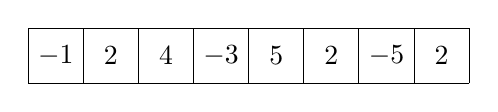
\begin{tikzpicture}[scale=0.7]
\draw (0,0) grid (8,1);

\node at (0.5,0.5) {$-1$};
\node at (1.5,0.5) {$2$};
\node at (2.5,0.5) {$4$};
\node at (3.5,0.5) {$-3$};
\node at (4.5,0.5) {$5$};
\node at (5.5,0.5) {$2$};
\node at (6.5,0.5) {$-5$};
\node at (7.5,0.5) {$2$};
\end{tikzpicture}
\end{center}
\begin{samepage}
以下子数组产生了最大和$10$：
\begin{center}
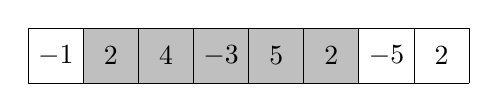
\begin{tikzpicture}[scale=0.7]
\fill[color=lightgray] (1,0) rectangle (6,1);
\draw (0,0) grid (8,1);

\node at (0.5,0.5) {$-1$};
\node at (1.5,0.5) {$2$};
\node at (2.5,0.5) {$4$};
\node at (3.5,0.5) {$-3$};
\node at (4.5,0.5) {$5$};
\node at (5.5,0.5) {$2$};
\node at (6.5,0.5) {$-5$};
\node at (7.5,0.5) {$2$};
\end{tikzpicture}
\end{center}
\end{samepage}

我们假设允许空子数组，
因此最大子数组和总是至少为$0$。

\subsubsection{算法1}

解决问题的一种直观方法是遍历所有可能的子数组，
计算每个子数组的值之和，并维护最大和。
以下代码实现了这个算法：

\begin{lstlisting}
int best = 0;
for (int a = 0; a < n; a++) {
    for (int b = a; b < n; b++) {
        int sum = 0;
        for (int k = a; k <= b; k++) {
            sum += array[k];
        }
        best = max(best,sum);
    }
}
cout << best << "\n";
\end{lstlisting}

变量\texttt{a}和\texttt{b}固定了子数组的
第一个和最后一个索引，
值之和计算到变量\texttt{sum}中。
变量\texttt{best}包含搜索过程中找到的最大和。

该算法的时间复杂度为$O(n^3)$，
因为它由三个遍历输入的嵌套循环组成。

\subsubsection{算法2}

通过去掉一个循环，很容易让算法1变得更高效。
这可以通过在子数组右端移动的同时计算和来实现。
结果如下代码：

\begin{lstlisting}
int best = 0;
for (int a = 0; a < n; a++) {
    int sum = 0;
    for (int b = a; b < n; b++) {
        sum += array[b];
        best = max(best,sum);
    }
}
cout << best << "\n";
\end{lstlisting}
这一改变后，时间复杂度为$O(n^2)$。

\subsubsection{算法3}

令人惊讶的是，可以在$O(n)$时间内解决该问题\footnote{在\cite{ben86}中，这个线性时间算法被归功于J. B. Kadane，
因此该算法有时被称为\index{Kadane算法} \key{Kadane算法}。}，这意味着只需一个循环即可。
其思想是，对于每个数组位置，
计算以该位置结尾的子数组的最大和。
之后，问题的答案就是这些和中的最大值。

考虑寻找以位置$k$结尾的最大和子数组的子问题。
有两种可能：
\begin{enumerate}
\item 子数组只包含位置$k$处的元素。
\item 子数组由一个以位置$k-1$结尾的子数组
加上位置$k$处的元素组成。
\end{enumerate}

在后者的情况下，由于我们要找到
和最大的子数组，
以位置$k-1$结尾的子数组也应该是和最大的。
因此，我们可以通过从左到右计算每个结束位置的最大子数组和，
来高效地解决问题。

以下代码实现了该算法：
\begin{lstlisting}
int best = 0, sum = 0;
for (int k = 0; k < n; k++) {
    sum = max(array[k],sum+array[k]);
    best = max(best,sum);
}
cout << best << "\n";
\end{lstlisting}

该算法只包含一个遍历输入的循环，
因此时间复杂度为$O(n)$。
这也是可能达到的最好时间复杂度，
因为解决该问题的任何算法
都必须至少检查所有数组元素一次。

\subsubsection{效率比较}

研究算法在实践中有多高效是很有趣的。
下表展示了上述算法在现代计算机上
对于不同$n$值的运行时间。

在每次测试中，输入是随机生成的。
读取输入所需的时间未被测量。

\begin{center}
\begin{tabular}{rrrr}
数组大小$n$ & 算法1 & 算法2 & 算法3 \\
\hline
$10^2$ & $0.0$秒 & $0.0$秒 & $0.0$秒 \\
$10^3$ & $0.1$秒 & $0.0$秒 & $0.0$秒 \\
$10^4$ & > $10.0$秒 & $0.1$秒 & $0.0$秒 \\
$10^5$ & > $10.0$秒 & $5.3$秒 & $0.0$秒 \\
$10^6$ & > $10.0$秒 & > $10.0$秒 & $0.0$秒 \\
$10^7$ & > $10.0$秒 & > $10.0$秒 & $0.0$秒 \\
\end{tabular}
\end{center}

比较结果显示，当输入大小较小时，
所有算法都是高效的，
但随着输入增大，算法之间的运行时间
会出现显著差异。
当$n=10^4$时，算法1变慢；
当$n=10^5$时，算法2变慢。
只有算法3能够瞬间处理
即使是最大的输入。

\chapter{排序}

\index{排序}

\key{排序}是一个基础的算法设计问题。
许多高效的算法将排序作为子程序，
因为如果元素已经是有序的，
处理数据通常会更容易。

例如，问题''一个数组是否包含
两个相等的元素？''使用排序很容易解决。
如果数组包含两个相等的元素，
排序后它们会相邻，
因此很容易找到它们。
同样，问题''数组中出现最频繁的元素是什么？''
也可以用类似的方法解决。

排序的算法有很多种，它们也是
应用不同算法设计技术的良好示例。
高效的通用排序算法
在$O(n \log n)$时间内完成，
许多使用排序作为子程序的算法
也具有这个时间复杂度。

\section{排序理论}

排序的基本问题如下：
\begin{framed}
\noindent
给定一个包含$n$个元素的数组，
你的任务是将元素
按递增顺序排序。
\end{framed}
\noindent
例如，数组
\begin{center}
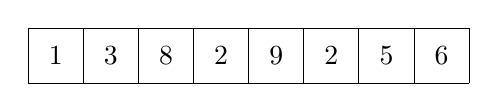
\begin{tikzpicture}[scale=0.7]
\draw (0,0) grid (8,1);
\node at (0.5,0.5) {$1$};
\node at (1.5,0.5) {$3$};
\node at (2.5,0.5) {$8$};
\node at (3.5,0.5) {$2$};
\node at (4.5,0.5) {$9$};
\node at (5.5,0.5) {$2$};
\node at (6.5,0.5) {$5$};
\node at (7.5,0.5) {$6$};
\end{tikzpicture}
\end{center}
排序后将变为：
\begin{center}
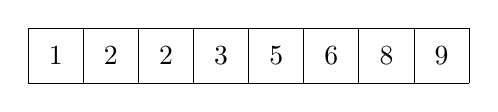
\begin{tikzpicture}[scale=0.7]
\draw (0,0) grid (8,1);
\node at (0.5,0.5) {$1$};
\node at (1.5,0.5) {$2$};
\node at (2.5,0.5) {$2$};
\node at (3.5,0.5) {$3$};
\node at (4.5,0.5) {$5$};
\node at (5.5,0.5) {$6$};
\node at (6.5,0.5) {$8$};
\node at (7.5,0.5) {$9$};
\end{tikzpicture}
\end{center}

\subsubsection{$O(n^2)$算法}

\index{冒泡排序}

简单的数组排序算法
在$O(n^2)$时间内完成。
这类算法很简短，通常
由两个嵌套循环组成。
一个著名的$O(n^2)$时间排序算法
是\key{冒泡排序}，其中元素根据其值
在数组中''冒泡''。

冒泡排序由$n$轮组成。
在每一轮中，算法遍历
数组的元素。
每当发现两个连续元素
的顺序不正确时，
算法就交换它们。
该算法可以实现如下：
\begin{lstlisting}
for (int i = 0; i < n; i++) {
    for (int j = 0; j < n-1; j++) {
        if (array[j] > array[j+1]) {
            swap(array[j],array[j+1]);
        }
    }
}
\end{lstlisting}

在算法的第一轮之后，
最大的元素将处于正确位置，
一般来说，经过$k$轮后，最大的$k$个
元素将处于正确位置。
因此，经过$n$轮后，整个数组
将被排序。

例如，在数组

\begin{center}
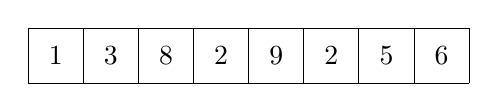
\begin{tikzpicture}[scale=0.7]
\draw (0,0) grid (8,1);

\node at (0.5,0.5) {$1$};
\node at (1.5,0.5) {$3$};
\node at (2.5,0.5) {$8$};
\node at (3.5,0.5) {$2$};
\node at (4.5,0.5) {$9$};
\node at (5.5,0.5) {$2$};
\node at (6.5,0.5) {$5$};
\node at (7.5,0.5) {$6$};
\end{tikzpicture}
\end{center}

\noindent
冒泡排序的第一轮交换元素
如下：

\begin{center}
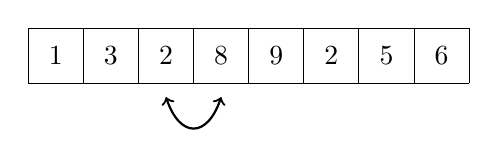
\begin{tikzpicture}[scale=0.7]
\draw (0,0) grid (8,1);
\node at (0.5,0.5) {$1$};
\node at (1.5,0.5) {$3$};
\node at (2.5,0.5) {$2$};
\node at (3.5,0.5) {$8$};
\node at (4.5,0.5) {$9$};
\node at (5.5,0.5) {$2$};
\node at (6.5,0.5) {$5$};
\node at (7.5,0.5) {$6$};

\draw[thick,<->] (3.5,-0.25) .. controls (3.25,-1.00) and (2.75,-1.00) .. (2.5,-0.25);
\end{tikzpicture}
\end{center}

\begin{center}
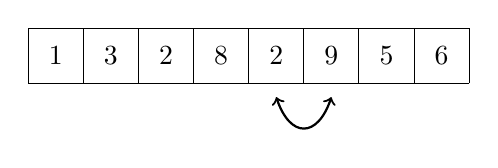
\begin{tikzpicture}[scale=0.7]
\draw (0,0) grid (8,1);
\node at (0.5,0.5) {$1$};
\node at (1.5,0.5) {$3$};
\node at (2.5,0.5) {$2$};
\node at (3.5,0.5) {$8$};
\node at (4.5,0.5) {$2$};
\node at (5.5,0.5) {$9$};
\node at (6.5,0.5) {$5$};
\node at (7.5,0.5) {$6$};

\draw[thick,<->] (5.5,-0.25) .. controls (5.25,-1.00) and (4.75,-1.00) .. (4.5,-0.25);
\end{tikzpicture}
\end{center}

\begin{center}
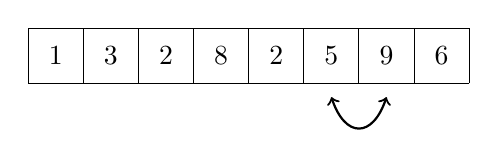
\begin{tikzpicture}[scale=0.7]
\draw (0,0) grid (8,1);
\node at (0.5,0.5) {$1$};
\node at (1.5,0.5) {$3$};
\node at (2.5,0.5) {$2$};
\node at (3.5,0.5) {$8$};
\node at (4.5,0.5) {$2$};
\node at (5.5,0.5) {$5$};
\node at (6.5,0.5) {$9$};
\node at (7.5,0.5) {$6$};

\draw[thick,<->] (6.5,-0.25) .. controls (6.25,-1.00) and (5.75,-1.00) .. (5.5,-0.25);
\end{tikzpicture}
\end{center}

\begin{center}
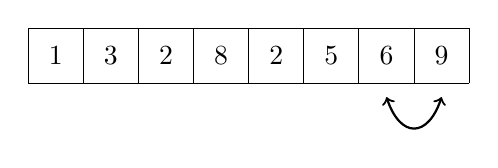
\begin{tikzpicture}[scale=0.7]
\draw (0,0) grid (8,1);
\node at (0.5,0.5) {$1$};
\node at (1.5,0.5) {$3$};
\node at (2.5,0.5) {$2$};
\node at (3.5,0.5) {$8$};
\node at (4.5,0.5) {$2$};
\node at (5.5,0.5) {$5$};
\node at (6.5,0.5) {$6$};
\node at (7.5,0.5) {$9$};

\draw[thick,<->] (7.5,-0.25) .. controls (7.25,-1.00) and (6.75,-1.00) .. (6.5,-0.25);
\end{tikzpicture}
\end{center}

\subsubsection{逆序对}

\index{逆序对}

冒泡排序是一种始终交换数组中\emph{相邻}
元素的排序算法的例子。
事实证明，这类算法的时间复杂度\emph{总是}
至少为$O(n^2)$，因为在最坏情况下，
排序数组需要$O(n^2)$次交换。

分析排序算法时的一个有用概念是\key{逆序对}：
一对数组元素
$(\texttt{array}[a],\texttt{array}[b])$，满足
$a<b$且$\texttt{array}[a]>\texttt{array}[b]$，
即元素的顺序是错误的。
例如，数组
\begin{center}
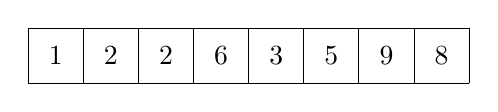
\begin{tikzpicture}[scale=0.7]
\draw (0,0) grid (8,1);
\node at (0.5,0.5) {$1$};
\node at (1.5,0.5) {$2$};
\node at (2.5,0.5) {$2$};
\node at (3.5,0.5) {$6$};
\node at (4.5,0.5) {$3$};
\node at (5.5,0.5) {$5$};
\node at (6.5,0.5) {$9$};
\node at (7.5,0.5) {$8$};
\end{tikzpicture}
\end{center}
有三个逆序对：$(6,3)$、$(6,5)$和$(9,8)$。
逆序对的数量表明
排序数组需要多少工作量。
当没有逆序对时，
数组完全有序。
另一方面，如果数组元素
是逆序排列的，
逆序对的数量达到最大：
\[1+2+\cdots+(n-1)=\frac{n(n-1)}{2} = O(n^2)\]

交换一对顺序错误的相邻元素
会从数组中恰好移除一个逆序对。
因此，如果排序算法只能交换相邻元素，
每次交换最多移除一个逆序对，
算法的时间复杂度至少为$O(n^2)$。

\subsubsection{$O(n \log n)$算法}

\index{归并排序}

使用不局限于交换相邻元素的算法，
可以在$O(n \log n)$时间内高效地对数组进行排序。
其中一个这样的算法是\key{归并排序}\footnote{根据\cite{knu983}，
归并排序由J. von Neumann于1945年发明。}，
它基于递归。

归并排序按如下方式对子数组\texttt{array}$[a \ldots b]$进行排序：

\begin{enumerate}
\item 如果$a=b$，不做任何操作，因为子数组已经有序。
\item 计算中间元素的位置：$k=\lfloor (a+b)/2 \rfloor$。
\item 递归排序子数组\texttt{array}$[a \ldots k]$。
\item 递归排序子数组\texttt{array}$[k+1 \ldots b]$。
\item 将已排序的子数组\texttt{array}$[a \ldots k]$和
\texttt{array}$[k+1 \ldots b]$
\emph{合并}为已排序的子数组\texttt{array}$[a \ldots b]$。
\end{enumerate}

归并排序是一个高效的算法，因为它
在每一步将子数组的大小减半。
递归由$O(\log n)$层组成，
处理每一层需要$O(n)$时间。
合并子数组\texttt{array}$[a \ldots k]$和\texttt{array}$[k+1 \ldots b]$
可以在线性时间内完成，因为它们已经有序。

例如，考虑对以下数组进行排序：
\begin{center}
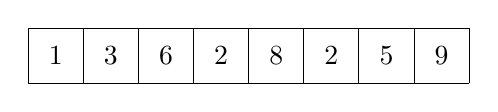
\begin{tikzpicture}[scale=0.7]
\draw (0,0) grid (8,1);
\node at (0.5,0.5) {$1$};
\node at (1.5,0.5) {$3$};
\node at (2.5,0.5) {$6$};
\node at (3.5,0.5) {$2$};
\node at (4.5,0.5) {$8$};
\node at (5.5,0.5) {$2$};
\node at (6.5,0.5) {$5$};
\node at (7.5,0.5) {$9$};
\end{tikzpicture}
\end{center}

数组将被分成两个子数组
如下：
\begin{center}
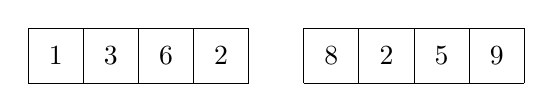
\begin{tikzpicture}[scale=0.7]
\draw (0,0) grid (4,1);
\draw (5,0) grid (9,1);

\node at (0.5,0.5) {$1$};
\node at (1.5,0.5) {$3$};
\node at (2.5,0.5) {$6$};
\node at (3.5,0.5) {$2$};

\node at (5.5,0.5) {$8$};
\node at (6.5,0.5) {$2$};
\node at (7.5,0.5) {$5$};
\node at (8.5,0.5) {$9$};
\end{tikzpicture}
\end{center}

然后，子数组将被递归排序
如下：
\begin{center}
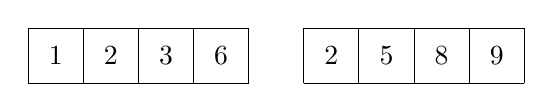
\begin{tikzpicture}[scale=0.7]
\draw (0,0) grid (4,1);
\draw (5,0) grid (9,1);

\node at (0.5,0.5) {$1$};
\node at (1.5,0.5) {$2$};
\node at (2.5,0.5) {$3$};
\node at (3.5,0.5) {$6$};

\node at (5.5,0.5) {$2$};
\node at (6.5,0.5) {$5$};
\node at (7.5,0.5) {$8$};
\node at (8.5,0.5) {$9$};
\end{tikzpicture}
\end{center}

最后，算法合并已排序的
子数组并创建最终排序的数组：
\begin{center}
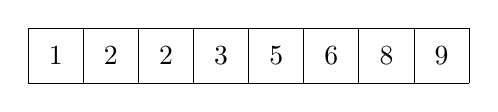
\begin{tikzpicture}[scale=0.7]
\draw (0,0) grid (8,1);
\node at (0.5,0.5) {$1$};
\node at (1.5,0.5) {$2$};
\node at (2.5,0.5) {$2$};
\node at (3.5,0.5) {$3$};
\node at (4.5,0.5) {$5$};
\node at (5.5,0.5) {$6$};
\node at (6.5,0.5) {$8$};
\node at (7.5,0.5) {$9$};
\end{tikzpicture}
\end{center}

\subsubsection{排序下界}

是否可能在快于
$O(n \log n)$的时间内对数组排序？
事实证明，当我们限定在基于比较数组元素的排序算法时，
这是\emph{不可能}的。

通过将排序视为一个过程——其中每次比较两个元素
都会给出关于数组内容的更多信息——
可以证明时间复杂度的下界。
该过程创建如下树：

\begin{center}
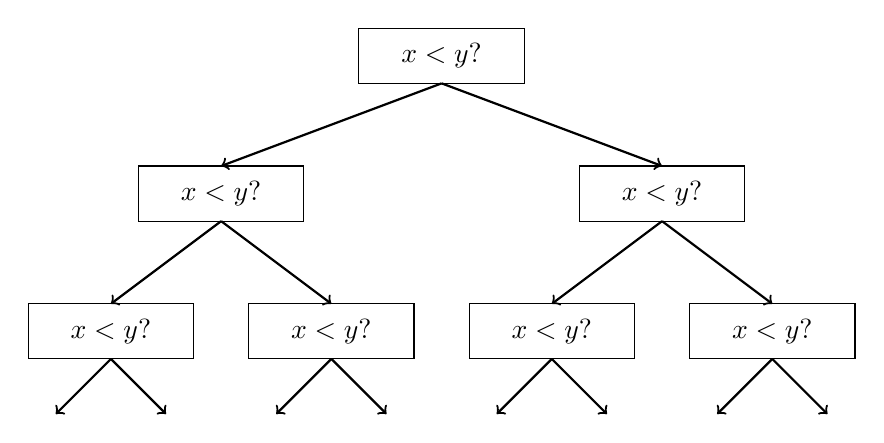
\begin{tikzpicture}[scale=0.7]
\draw (0,0) rectangle (3,1);
\node at (1.5,0.5) {$x < y?$};

\draw[thick,->] (1.5,0) -- (-2.5,-1.5);
\draw[thick,->] (1.5,0) -- (5.5,-1.5);

\draw (-4,-2.5) rectangle (-1,-1.5);
\draw (4,-2.5) rectangle (7,-1.5);
\node at (-2.5,-2) {$x < y?$};
\node at (5.5,-2) {$x < y?$};

\draw[thick,->] (-2.5,-2.5) -- (-4.5,-4);
\draw[thick,->] (-2.5,-2.5) -- (-0.5,-4);
\draw[thick,->] (5.5,-2.5) -- (3.5,-4);
\draw[thick,->] (5.5,-2.5) -- (7.5,-4);

\draw (-6,-5) rectangle (-3,-4);
\draw (-2,-5) rectangle (1,-4);
\draw (2,-5) rectangle (5,-4);
\draw (6,-5) rectangle (9,-4);
\node at (-4.5,-4.5) {$x < y?$};
\node at (-0.5,-4.5) {$x < y?$};
\node at (3.5,-4.5) {$x < y?$};
\node at (7.5,-4.5) {$x < y?$};

\draw[thick,->] (-4.5,-5) -- (-5.5,-6);
\draw[thick,->] (-4.5,-5) -- (-3.5,-6);
\draw[thick,->] (-0.5,-5) -- (0.5,-6);
\draw[thick,->] (-0.5,-5) -- (-1.5,-6);
\draw[thick,->] (3.5,-5) -- (2.5,-6);
\draw[thick,->] (3.5,-5) -- (4.5,-6);
\draw[thick,->] (7.5,-5) -- (6.5,-6);
\draw[thick,->] (7.5,-5) -- (8.5,-6);
\end{tikzpicture}
\end{center}

这里''$x<y?$''表示比较某些元素
$x$和$y$。
如果$x<y$，过程继续向左，
否则向右。
过程的结果是排序数组的可能方式，
总共有$n!$种。
因此，树的高度必须至少为
\[ \log_2(n!) = \log_2(1)+\log_2(2)+\cdots+\log_2(n).\]
我们通过选择最后的$n/2$个元素
并将每个元素的值改为$\log_2(n/2)$
来得到这个和的下界。
这给出了一个估计
\[ \log_2(n!) \ge (n/2) \cdot \log_2(n/2),\]
所以树的高度以及排序算法在最坏情况下
可能的最少步数
至少为$n \log n$。

\subsubsection{计数排序}

\index{计数排序}

下界$n \log n$不适用于
不比较数组元素而是使用其他信息的算法。
这种算法的一个例子是
\key{计数排序}，它在$O(n)$时间内对数组排序，
前提是数组中的每个元素
都是$0 \ldots c$之间的整数且$c=O(n)$。

该算法创建一个\emph{簿记}数组，
其索引是原始数组的元素。
算法遍历原始数组
并计算每个元素在数组中
出现的次数。
\newpage

例如，数组
\begin{center}
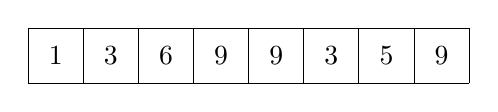
\begin{tikzpicture}[scale=0.7]
\draw (0,0) grid (8,1);
\node at (0.5,0.5) {$1$};
\node at (1.5,0.5) {$3$};
\node at (2.5,0.5) {$6$};
\node at (3.5,0.5) {$9$};
\node at (4.5,0.5) {$9$};
\node at (5.5,0.5) {$3$};
\node at (6.5,0.5) {$5$};
\node at (7.5,0.5) {$9$};
\end{tikzpicture}
\end{center}
对应以下簿记数组：
\begin{center}
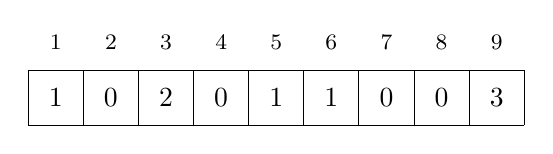
\begin{tikzpicture}[scale=0.7]
\draw (0,0) grid (9,1);
\node at (0.5,0.5) {$1$};
\node at (1.5,0.5) {$0$};
\node at (2.5,0.5) {$2$};
\node at (3.5,0.5) {$0$};
\node at (4.5,0.5) {$1$};
\node at (5.5,0.5) {$1$};
\node at (6.5,0.5) {$0$};
\node at (7.5,0.5) {$0$};
\node at (8.5,0.5) {$3$};

\footnotesize

\node at (0.5,1.5) {$1$};
\node at (1.5,1.5) {$2$};
\node at (2.5,1.5) {$3$};
\node at (3.5,1.5) {$4$};
\node at (4.5,1.5) {$5$};
\node at (5.5,1.5) {$6$};
\node at (6.5,1.5) {$7$};
\node at (7.5,1.5) {$8$};
\node at (8.5,1.5) {$9$};
\end{tikzpicture}
\end{center}

例如，簿记数组中位置3的值
为2，因为元素3在原始数组中
出现了2次。

构造簿记数组需要$O(n)$时间。
之后，可以在$O(n)$时间内创建排序后的数组，
因为可以从簿记数组中
获取每个元素的出现次数。
因此，计数排序的总时间复杂度为$O(n)$。

计数排序是一个非常高效的算法，
但它只能在常数$c$足够小的时候使用，
以便数组元素可以用作簿记数组的索引。

\section{C++中的排序}

\index{sort@\texttt{sort}}

在竞赛中几乎从不是一个好主意
去使用自制排序算法，
因为编程语言中已经有了
很好的实现。
例如，C++标准库包含
函数\texttt{sort}，可以轻松用于
对数组和其他数据结构进行排序。

使用库函数有很多好处。
首先，它节省时间，因为不需要
实现该函数。
其次，库的实现肯定是正确且高效的：
自制的排序函数不太可能更好。

在本节中，我们将看到如何使用
C++ \texttt{sort}函数。
以下代码按递增顺序对
向量进行排序：
\begin{lstlisting}
vector<int> v = {4,2,5,3,5,8,3};
sort(v.begin(),v.end());
\end{lstlisting}
排序后，向量的内容将变为
$[2,3,3,4,5,5,8]$。
默认排序顺序是递增的，
但可以按如下方式使用逆序：
\begin{lstlisting}
sort(v.rbegin(),v.rend());
\end{lstlisting}
普通数组可以按如下方式排序：
\begin{lstlisting}
int n = 7; // 数组大小
int a[] = {4,2,5,3,5,8,3};
sort(a,a+n);
\end{lstlisting}
\newpage
以下代码对字符串\texttt{s}进行排序：
\begin{lstlisting}
string s = "monkey";
sort(s.begin(), s.end());
\end{lstlisting}
对字符串进行排序意味着
对字符串的字符进行排序。
例如，字符串''monkey''变为''ekmnoy''。

\subsubsection{比较运算符}

\index{比较运算符}

函数\texttt{sort}要求为待排序元素的数据类型
定义\key{比较运算符}。
排序时，每当需要确定两个元素的顺序时，
就会使用该运算符。

大多数C++数据类型都有内置的比较运算符，
这些类型的元素可以自动排序。
例如，数字按值排序，
字符串按字母顺序排序。

\index{pair@\texttt{pair}}

对（\texttt{pair}）首先根据其
第一个元素（\texttt{first}）排序。
但是，如果两个对的第一个元素相等，
则根据第二个元素（\texttt{second}）排序：
\begin{lstlisting}
vector<pair<int,int>> v;
v.push_back({1,5});
v.push_back({2,3});
v.push_back({1,2});
sort(v.begin(), v.end());
\end{lstlisting}
之后，对的顺序为
$(1,2)$、$(1,5)$和$(2,3)$。

\index{tuple@\texttt{tuple}}

以类似的方式，元组（\texttt{tuple}）
首先按第一个元素排序，
其次按第二个元素排序，以此类推。\footnote{注意，在一些较旧的编译器中，
必须使用函数\texttt{make\_tuple}来创建元组，
而不是使用花括号（例如，\texttt{make\_tuple(2,1,4)}而不是\texttt{\{2,1,4\}}）。}：
\begin{lstlisting}
vector<tuple<int,int,int>> v;
v.push_back({2,1,4});
v.push_back({1,5,3});
v.push_back({2,1,3});
sort(v.begin(), v.end());
\end{lstlisting}
之后，元组的顺序为
$(1,5,3)$、$(2,1,3)$和$(2,1,4)$。

\subsubsection{用户自定义结构体}

用户自定义结构体不会自动拥有
比较运算符。
该运算符应该在结构体内部
定义为函数\texttt{operator<}，
其参数是同一类型的另一个元素。
如果元素小于参数，
运算符应返回\texttt{true}，
否则返回\texttt{false}。

例如，以下结构体\texttt{P}
包含一个点的x和y坐标。
比较运算符定义为
首先按x坐标排序，
其次按y坐标排序。

\begin{lstlisting}
struct P {
    int x, y;
    bool operator<(const P &p) {
        if (x != p.x) return x < p.x;
        else return y < p.y;
    }
};
\end{lstlisting}

\subsubsection{比较函数}

\index{比较函数}

还可以将外部
\key{比较函数}作为回调函数
传递给\texttt{sort}函数。
例如，以下比较函数\texttt{comp}
首先按字符串长度排序，
其次按字母顺序排序：

\begin{lstlisting}
bool comp(string a, string b) {
    if (a.size() != b.size()) return a.size() < b.size();
    return a < b;
}
\end{lstlisting}
现在可以按如下方式对字符串向量进行排序：
\begin{lstlisting}
sort(v.begin(), v.end(), comp);
\end{lstlisting}

\section{二分查找}

\index{二分查找}

在数组中搜索元素的通用方法是
使用\texttt{for}循环
遍历数组的元素。
例如，以下代码在数组中
搜索元素$x$：

\begin{lstlisting}
for (int i = 0; i < n; i++) {
    if (array[i] == x) {
        // 在索引i处找到x
    }
}
\end{lstlisting}

这种方法的时间复杂度为$O(n)$，
因为在最坏情况下，需要检查
数组的所有元素。
如果元素的顺序是任意的，
这也是最好的方法，因为没有额外的信息
表明应该在数组的哪里搜索元素$x$。

但是，如果数组是\emph{有序的}，
情况就不同了。
在这种情况下，可以更快地执行
搜索，因为数组中元素的顺序
会指引搜索。
以下\key{二分查找}算法
可以在$O(\log n)$时间内高效地
在有序数组中搜索元素。

\subsubsection{方法1}

二分查找的通常实现方式
类似于在字典中查找一个单词。
搜索在数组中维护一个活动区间，
初始时包含数组的所有元素。
然后，执行若干步骤，
每一步将区间的大小减半。

在每一步中，搜索检查活动区间
的中间元素。
如果中间元素就是目标元素，
搜索终止。
否则，搜索根据中间元素的值
递归地继续到区间的左半部分
或右半部分。

上述思路可以实现如下：
\begin{lstlisting}
int a = 0, b = n-1;
while (a <= b) {
    int k = (a+b)/2;
    if (array[k] == x) {
        // 在索引k处找到x
    }
    if (array[k] > x) b = k-1;
    else a = k+1;
}
\end{lstlisting}

在这个实现中，活动区间是$a \ldots b$，
初始区间为$0 \ldots n-1$。
算法在每一步将区间大小减半，
因此时间复杂度为$O(\log n)$。

\subsubsection{方法2}

另一种实现二分查找的方法
基于一种高效遍历数组元素的方式。
思路是进行跳跃，并在
接近目标元素时减慢速度。

搜索从左到右遍历数组，
初始跳跃长度为$n/2$。
在每一步中，跳跃长度将减半：
首先是$n/4$，然后是$n/8$、$n/16$等，
直到最后长度为1。
跳跃结束后，要么找到了目标元素，
要么我们知道它不在数组中。

以下代码实现了上述思想：
\begin{lstlisting}
int k = 0;
for (int b = n/2; b >= 1; b /= 2) {
    while (k+b < n && array[k+b] <= x) k += b;
}
if (array[k] == x) {
    // 在索引k处找到x
}
\end{lstlisting}

在搜索过程中，变量$b$
包含当前跳跃长度。
算法的时间复杂度为$O(\log n)$，
因为\texttt{while}循环中的代码
对每个跳跃长度最多执行两次。

\subsubsection{C++函数}

C++标准库包含以下基于二分查找的函数，
它们在对数时间内工作：

\begin{itemize}
\item \texttt{lower\_bound}返回指向
值不小于$x$的第一个数组元素的指针。
\item \texttt{upper\_bound}返回指向
值大于$x$的第一个数组元素的指针。
\item \texttt{equal\_range}返回上述两个指针。
\end{itemize}

这些函数假设数组是有序的。
如果不存在这样的元素，指针指向
数组最后一个元素之后的位置。
例如，以下代码判断
数组是否包含值为$x$的元素：

\begin{lstlisting}
auto k = lower_bound(array,array+n,x)-array;
if (k < n && array[k] == x) {
    // 在索引 k 处找到 x
}
\end{lstlisting}

然后，以下代码统计值为 $x$ 的元素个数：

\begin{lstlisting}
auto a = lower_bound(array, array+n, x);
auto b = upper_bound(array, array+n, x);
cout << b-a << "\n";
\end{lstlisting}

使用\texttt{equal\_range}，代码变得更简洁：

\begin{lstlisting}
auto r = equal_range(array, array+n, x);
cout << r.second-r.first << "\n";
\end{lstlisting}

\subsubsection{寻找最小解}

二分查找的一个重要用途是
找到\emph{函数}值发生变化的位置。
假设我们希望找到某个问题的
最小值$k$，使得它是有效解。
给定一个函数$\texttt{ok}(x)$，
如果$x$是有效解则返回\texttt{true}，
否则返回\texttt{false}。
此外，我们知道当$x<k$时$\texttt{ok}(x)$为\texttt{false}，
当$x \ge k$时为\texttt{true}。
情况如下：

\begin{center}
\begin{tabular}{r|rrrrrrrr}
$x$ & 0 & 1 & $\cdots$ & $k-1$ & $k$ & $k+1$ & $\cdots$ \\
\hline
$\texttt{ok}(x)$ & \texttt{false} & \texttt{false}
& $\cdots$ & \texttt{false} & \texttt{true} & \texttt{true} & $\cdots$ \\
\end{tabular}
\end{center}

\noindent
现在，可以使用二分查找找到$k$的值：

\begin{lstlisting}
int x = -1;
for (int b = z; b >= 1; b /= 2) {
    while (!ok(x+b)) x += b;
}
int k = x+1;
\end{lstlisting}

搜索找到最大的$x$值，使得
$\texttt{ok}(x)$为\texttt{false}。
因此，下一个值$k=x+1$
是使$\texttt{ok}(k)$为\texttt{true}
的最小可能值。
初始跳跃长度$z$必须
足够大，例如我们事先已知
$\texttt{ok}(z)$为\texttt{true}的某个值。

算法调用函数\texttt{ok}
$O(\log z)$次，因此总时间复杂度
取决于函数\texttt{ok}。
例如，如果该函数在$O(n)$时间内工作，
则总时间复杂度为$O(n \log z)$。

\subsubsection{寻找最大值}

二分查找也可以用于找到一个
先递增后递减的函数的最大值。
我们的任务是找到位置$k$，使得

\begin{itemize}
\item
当$x<k$时$f(x)<f(x+1)$，且
\item
当$x \ge k$时$f(x)>f(x+1)$。
\end{itemize}

思路是使用二分查找
找到最大的$x$值
使得$f(x)<f(x+1)$。
这意味着$k=x+1$，
因为$f(x+1)>f(x+2)$。
以下代码实现了该搜索： 

\begin{lstlisting}
int x = -1;
for (int b = z; b >= 1; b /= 2) {
    while (f(x+b) < f(x+b+1)) x += b;
}
int k = x+1;
\end{lstlisting}

注意，与普通二分查找不同，
这里不允许函数的连续值
相等。
在这种情况下，无法知道
如何继续搜索。

\chapter{数据结构}

\index{数据结构}

\key{数据结构}是一种在计算机内存中存储数据的方式。
为问题选择合适的数据结构非常重要，
因为每种数据结构都有其自身的
优势和劣势。
关键问题是：在所选的数据结构中，
哪些操作是高效的？

本章介绍C++标准库中最重要的数据结构。
尽可能使用标准库是一个好习惯，
因为它可以节省大量时间。
在本书的后半部分，我们将学习标准库中
没有提供的更高级的数据结构。

\section{动态数组}

\index{动态数组}
\index{vector}

\key{动态数组}是一种大小可以在程序执行过程中
改变的数据结构。
C++中最常用的动态数组是
\texttt{vector}结构，
它的使用方式几乎和普通数组一样。

以下代码创建一个空vector并向其中添加三个元素：

\begin{lstlisting}
vector<int> v;
v.push_back(3); // [3]
v.push_back(2); // [3,2]
v.push_back(5); // [3,2,5]
\end{lstlisting}

此后，可以像普通数组一样访问元素：

\begin{lstlisting}
cout << v[0] << "\n"; // 3
cout << v[1] << "\n"; // 2
cout << v[2] << "\n"; // 5
\end{lstlisting}

函数\texttt{size}返回vector中元素的数量。
以下代码遍历vector并打印其中的所有元素：

\begin{lstlisting}
for (int i = 0; i < v.size(); i++) {
    cout << v[i] << "\n";
}
\end{lstlisting}

\begin{samepage}
遍历vector的一种更简洁的方式如下：

\begin{lstlisting}
for (auto x : v) {
    cout << x << "\n";
}
\end{lstlisting}
\end{samepage}

函数\texttt{back}返回vector中的最后一个元素，
函数\texttt{pop\_back}移除最后一个元素：

\begin{lstlisting}
vector<int> v;
v.push_back(5);
v.push_back(2);
cout << v.back() << "\n"; // 2
v.pop_back();
cout << v.back() << "\n"; // 5
\end{lstlisting}

以下代码创建一个包含五个元素的vector：

\begin{lstlisting}
vector<int> v = {2,4,2,5,1};
\end{lstlisting}

创建vector的另一种方式是指定元素的数量
和每个元素的初始值：

\begin{lstlisting}
// 大小为10，初始值为0
vector<int> v(10);
\end{lstlisting}
\begin{lstlisting}
// 大小为10，初始值为5
vector<int> v(10, 5);
\end{lstlisting}

vector的内部实现使用的是普通数组。
如果vector的大小增加导致数组变得太小，
就会分配一个新的数组，并将所有元素
移动到新数组中。
然而，这种情况并不经常发生，
\texttt{push\_back}的平均时间复杂度为$O(1)$。

\index{string}

\texttt{string}结构
也是一种动态数组，其使用方式几乎与vector相同。
此外，字符串有一些其他数据结构所没有的特殊语法。
字符串可以使用\texttt{+}符号进行拼接。
函数$\texttt{substr}(k,x)$返回从位置$k$开始、
长度为$x$的子串，
函数$\texttt{find}(\texttt{t})$查找子串\texttt{t}第一次出现的位置。

以下代码展示了一些字符串操作：

\begin{lstlisting}
string a = "hatti";
string b = a+a;
cout << b << "\n"; // hattihatti
b[5] = 'v';
cout << b << "\n"; // hattivatti
string c = b.substr(3,4);
cout << c << "\n"; // tiva
\end{lstlisting}

\section{集合结构}

\index{set}

\key{集合}是一种维护一组元素的数据结构。
集合的基本操作包括元素
插入、查找和删除。

C++标准库包含两种集合实现：
\texttt{set}结构基于平衡二叉树，
其操作的时间复杂度为$O(\log n)$。
\texttt{unordered\_set}结构使用哈希，
其操作的平均时间复杂度为$O(1)$。

选择哪种集合实现通常是个人偏好的问题。
\texttt{set}结构的优势在于它能维护元素的顺序，
并提供\texttt{unordered\_set}中不可用的函数。
另一方面，\texttt{unordered\_set}
可能更高效。

以下代码创建一个包含整数的集合，
并展示了一些操作。
函数\texttt{insert}向集合中添加元素，
函数\texttt{count}返回元素在集合中出现的次数，
函数\texttt{erase}从集合中移除元素。

\begin{lstlisting}
set<int> s;
s.insert(3);
s.insert(2);
s.insert(5);
cout << s.count(3) << "\n"; // 1
cout << s.count(4) << "\n"; // 0
s.erase(3);
s.insert(4);
cout << s.count(3) << "\n"; // 0
cout << s.count(4) << "\n"; // 1
\end{lstlisting}

集合的使用方式大体上与vector类似，
但不能使用\texttt{[]}语法来访问元素。
以下代码创建一个集合，
打印其中元素的数量，然后遍历所有元素：
\begin{lstlisting}
set<int> s = {2,5,6,8};
cout << s.size() << "\n"; // 4
for (auto x : s) {
    cout << x << "\n";
}
\end{lstlisting}

集合的一个重要性质是
所有元素都是\emph{互异的}。
因此，函数\texttt{count}总是返回
0（元素不在集合中）
或1（元素在集合中），
而函数\texttt{insert}在元素已存在时
不会再次添加。
以下代码说明了这一点：

\begin{lstlisting}
set<int> s;
s.insert(5);
s.insert(5);
s.insert(5);
cout << s.count(5) << "\n"; // 1
\end{lstlisting}

C++还包含\texttt{multiset}和\texttt{unordered\_multiset}结构，
它们的使用方式与\texttt{set}
和\texttt{unordered\_set}类似，
但它们可以包含同一个元素的多个实例。
例如，以下代码将数字5的三个实例
都添加到一个multiset中：

\begin{lstlisting}
multiset<int> s;
s.insert(5);
s.insert(5);
s.insert(5);
cout << s.count(5) << "\n"; // 3
\end{lstlisting}
函数\texttt{erase}会从multiset中
移除一个元素的所有实例：
\begin{lstlisting}
s.erase(5);
cout << s.count(5) << "\n"; // 0
\end{lstlisting}
通常，只需要移除一个实例，
可以按如下方式实现：
\begin{lstlisting}
s.erase(s.find(5));
cout << s.count(5) << "\n"; // 2
\end{lstlisting}

\section{映射结构}

\index{map}

\key{映射}是一种广义数组，
由键值对组成。
普通数组的键总是连续的整数$0,1,\ldots,n-1$，
其中$n$是数组的大小，
而映射的键可以是任何数据类型，
且不需要是连续的值。

C++标准库包含两种映射实现，
与集合的实现相对应：
\texttt{map}结构基于平衡二叉树，
访问元素的时间复杂度为$O(\log n)$，
而\texttt{unordered\_map}结构使用哈希，
访问元素的平均时间复杂度为$O(1)$。

以下代码创建一个键为字符串、值为整数的映射：

\begin{lstlisting}
map<string,int> m;
m["monkey"] = 4;
m["banana"] = 3;
m["harpsichord"] = 9;
cout << m["banana"] << "\n"; // 3
\end{lstlisting}

如果请求一个键的值，
但映射中不包含该键，
则该键会自动添加到映射中并赋予默认值。
例如，在以下代码中，
键''aybabtu''的值0被添加到映射中。

\begin{lstlisting}
map<string,int> m;
cout << m["aybabtu"] << "\n"; // 0
\end{lstlisting}
函数\texttt{count}检查映射中
是否存在某个键：
\begin{lstlisting}
if (m.count("aybabtu")) {
    // 键存在
}
\end{lstlisting}
以下代码打印映射中所有的键和值：
\begin{lstlisting}
for (auto x : m) {
    cout << x.first << " " << x.second << "\n";
}
\end{lstlisting}

\section{迭代器与范围}

\index{迭代器}

C++标准库中的许多函数都使用迭代器来操作。
\key{迭代器}是一个指向
数据结构中某个元素的变量。

常用的迭代器\texttt{begin}
和\texttt{end}定义了一个范围，
该范围包含数据结构中的所有元素。
迭代器\texttt{begin}指向数据结构中的第一个元素，
而迭代器\texttt{end}指向最后一个元素\emph{之后}的位置。
情况如下图所示：

\begin{center}
\begin{tabular}{llllllllll}
\{ & 3, & 4, & 6, & 8, & 12, & 13, & 14, & 17 & \} \\
& $\uparrow$ & & & & & & & & $\uparrow$ \\
& \multicolumn{3}{l}{\texttt{s.begin()}} & & & & & & \texttt{s.end()} \\
\end{tabular}
\end{center}

注意迭代器中的不对称性：
\texttt{s.begin()}指向数据结构中的一个元素，
而\texttt{s.end()}指向数据结构之外。
因此，迭代器定义的范围是\emph{半开}的。

\subsubsection{范围操作}

迭代器用于C++标准库中那些需要接收数据结构中
一个元素范围的函数。
通常，我们希望处理数据结构中的所有元素，
因此需要为函数提供\texttt{begin}和\texttt{end}迭代器。

例如，以下代码使用函数\texttt{sort}对一个vector排序，
然后使用函数\texttt{reverse}反转元素的顺序，
最后使用函数\texttt{random\_shuffle}随机打乱元素的顺序。

\index{sort@\texttt{sort}}
\index{reverse@\texttt{reverse}}
\index{random\_shuffle@\texttt{random\_shuffle}}

\begin{lstlisting}
sort(v.begin(), v.end());
reverse(v.begin(), v.end());
random_shuffle(v.begin(), v.end());
\end{lstlisting}

这些函数也可以用于普通数组。
在这种情况下，需要为数组提供指针
而不是迭代器：

\newpage
\begin{lstlisting}
sort(a, a+n);
reverse(a, a+n);
random_shuffle(a, a+n);
\end{lstlisting}

\subsubsection{集合迭代器}

迭代器常用于访问集合中的元素。
以下代码创建一个迭代器\texttt{it}，
指向集合中最小的元素：
\begin{lstlisting}
set<int>::iterator it = s.begin();
\end{lstlisting}
一种更简洁的写法如下：
\begin{lstlisting}
auto it = s.begin();
\end{lstlisting}
可以使用\texttt{*}符号访问迭代器所指向的元素。
例如，以下代码打印集合中的第一个元素：

\begin{lstlisting}
auto it = s.begin();
cout << *it << "\n";
\end{lstlisting}

可以使用运算符\texttt{++}（向前）和\texttt{--}（向后）
来移动迭代器，
即迭代器会移动到集合中的下一个或上一个元素。

以下代码按递增顺序打印所有元素：
\begin{lstlisting}
for (auto it = s.begin(); it != s.end(); it++) {
    cout << *it << "\n";
}
\end{lstlisting}
以下代码打印集合中最大的元素：
\begin{lstlisting}
auto it = s.end(); it--;
cout << *it << "\n";
\end{lstlisting}

函数$\texttt{find}(x)$返回一个
指向值为$x$的元素的迭代器。
但如果集合中不包含$x$，
迭代器将为\texttt{end}。

\begin{lstlisting}
auto it = s.find(x);
if (it == s.end()) {
    // 未找到x
}
\end{lstlisting}

函数$\texttt{lower\_bound}(x)$返回
一个迭代器，指向集合中值\emph{至少为}$x$的最小元素，
函数$\texttt{upper\_bound}(x)$
返回一个迭代器，指向集合中值\emph{大于}$x$的最小元素。
在两个函数中，如果这样的元素不存在，
返回值均为\texttt{end}。
这两个函数不被\texttt{unordered\_set}结构支持，
因为该结构不维护元素的顺序。

\begin{samepage}
例如，以下代码查找最接近$x$的元素：

\begin{lstlisting}
auto it = s.lower_bound(x);
if (it == s.begin()) {
    cout << *it << "\n";
} else if (it == s.end()) {
    it--;
    cout << *it << "\n";
} else {
    int a = *it; it--;
    int b = *it;
    if (x-b < a-x) cout << b << "\n";
    else cout << a << "\n";
}
\end{lstlisting}

该代码假设集合不为空，
并使用迭代器\texttt{it}遍历所有可能的情况。
首先，迭代器指向值至少为$x$的最小元素。
如果\texttt{it}等于\texttt{begin}，
则对应的元素最接近$x$。
如果\texttt{it}等于\texttt{end}，
则集合中最大的元素最接近$x$。
如果以上情况都不成立，
最接近$x$的元素要么是\texttt{it}对应的元素，
要么是前一个元素。
\end{samepage}

\section{其他结构}

\subsubsection{Bitset}

\index{bitset}

\key{bitset（位集）}是一种每个值
只能是0或1的数组。
例如，以下代码创建一个包含10个元素的bitset：
\begin{lstlisting}
bitset<10> s;
s[1] = 1;
s[3] = 1;
s[4] = 1;
s[7] = 1;
cout << s[4] << "\n"; // 1
cout << s[5] << "\n"; // 0
\end{lstlisting}

使用bitset的优势在于
它们比普通数组占用更少的内存，
因为bitset中的每个元素只占用一位内存。
例如，
如果将$n$个位存储在\texttt{int}数组中，
将使用$32n$位内存，
而相应的bitset只需$n$位内存。
此外，bitset的值可以使用位运算高效操作，
这使得用位集优化算法成为可能。

以下代码展示了创建上述bitset的另一种方式：
\begin{lstlisting}
bitset<10> s(string("0010011010")); // 从右到左
cout << s[4] << "\n"; // 1
cout << s[5] << "\n"; // 0
\end{lstlisting}

函数\texttt{count}返回
bitset中1的个数：

\begin{lstlisting}
bitset<10> s(string("0010011010"));
cout << s.count() << "\n"; // 4
\end{lstlisting}

以下代码展示了位运算的使用示例：
\begin{lstlisting}
bitset<10> a(string("0010110110"));
bitset<10> b(string("1011011000"));
cout << (a&b) << "\n"; // 0010010000
cout << (a|b) << "\n"; // 1011111110
cout << (a^b) << "\n"; // 1001101110
\end{lstlisting}

\subsubsection{Deque}

\index{deque}

\key{deque（双端队列）}是一种动态数组，
其大小可以在数组的两端高效地改变。
与vector一样，deque提供了函数
\texttt{push\_back}和\texttt{pop\_back}，
但它还包含了vector中不可用的函数
\texttt{push\_front}和\texttt{pop\_front}。

deque的使用方式如下：
\begin{lstlisting}
deque<int> d;
d.push_back(5); // [5]
d.push_back(2); // [5,2]
d.push_front(3); // [3,5,2]
d.pop_back(); // [3,5]
d.pop_front(); // [5]
\end{lstlisting}

deque的内部实现比vector更复杂，
因此deque比vector更慢。
不过，在两端添加和移除元素的平均时间复杂度均为$O(1)$。

\subsubsection{Stack}

\index{stack}

\key{stack（栈）}
是一种提供两种$O(1)$时间操作的数据结构：
在顶部添加元素，
以及从顶部移除元素。
只能访问栈顶的元素。

以下代码展示了如何使用栈：
\begin{lstlisting}
stack<int> s;
s.push(3);
s.push(2);
s.push(5);
cout << s.top(); // 5
s.pop();
cout << s.top(); // 2
\end{lstlisting}
\subsubsection{Queue}

\index{queue}

\key{queue（队列）}也提供两种$O(1)$时间操作：
在队列末尾添加元素，
以及移除队列中的第一个元素。
只能访问队列的第一个和最后一个元素。

以下代码展示了如何使用队列：
\begin{lstlisting}
queue<int> q;
q.push(3);
q.push(2);
q.push(5);
cout << q.front(); // 3
q.pop();
cout << q.front(); // 2
\end{lstlisting}

\subsubsection{优先队列}

\index{优先队列}
\index{堆}

\key{优先队列}（priority queue）
维护一组元素。
支持的操作包括插入，以及根据队列类型
检索和移除最小或最大元素。
插入和移除的时间复杂度为$O(\log n)$，
检索的时间复杂度为$O(1)$。

虽然有序集合也能高效支持优先队列的所有操作，
但使用优先队列的优势在于它的常数因子更小。
优先队列通常使用堆结构实现，
这比有序集合中使用的平衡二叉树简单得多。

\begin{samepage}
默认情况下，C++优先队列中的元素
按递减顺序排列，
可以查找和移除队列中最大的元素。
以下代码说明了这一点：

\begin{lstlisting}
priority_queue<int> q;
q.push(3);
q.push(5);
q.push(7);
q.push(2);
cout << q.top() << "\n"; // 7
q.pop();
cout << q.top() << "\n"; // 5
q.pop();
q.push(6);
cout << q.top() << "\n"; // 6
q.pop();
\end{lstlisting}
\end{samepage}

如果我们想创建一个支持查找和移除
最小元素的优先队列，
可以按如下方式实现：

\begin{lstlisting}
priority_queue<int,vector<int>,greater<int>> q;
\end{lstlisting}

\subsubsection{基于策略的数据结构}

\texttt{g++}编译器还支持
一些不属于C++标准库的数据结构。
这些结构被称为\emph{基于策略的}数据结构。
要使用这些结构，必须在代码中添加以下行：
\begin{lstlisting}
#include <ext/pb_ds/assoc_container.hpp>
using namespace __gnu_pbds; 
\end{lstlisting}
此后，我们可以定义一个数据结构\texttt{indexed\_set}，
它类似于\texttt{set}，但可以像数组一样进行索引。
对于\texttt{int}值的定义如下：
\begin{lstlisting}
typedef tree<int,null_type,less<int>,rb_tree_tag,
             tree_order_statistics_node_update> indexed_set; 
\end{lstlisting}
现在我们可以按如下方式创建一个集合：
\begin{lstlisting}
indexed_set s;
s.insert(2);
s.insert(3);
s.insert(7);
s.insert(9);
\end{lstlisting}
这个集合的特殊之处在于，我们可以访问
元素在有序数组中对应的索引。
函数$\texttt{find\_by\_order}$返回
指向给定位置元素的迭代器：
\begin{lstlisting}
auto x = s.find_by_order(2);
cout << *x << "\n"; // 7
\end{lstlisting}
函数$\texttt{order\_of\_key}$
返回给定元素的位置：
\begin{lstlisting}
cout << s.order_of_key(7) << "\n"; // 2
\end{lstlisting}
如果元素不在集合中，
我们得到的是该元素在集合中
将会处于的位置：
\begin{lstlisting}
cout << s.order_of_key(6) << "\n"; // 2
cout << s.order_of_key(8) << "\n"; // 3
\end{lstlisting}
这两个函数都以对数时间运行。

\section{与排序的比较}

通常可以用数据结构或排序来解决同一个问题。
有时这两种方法的实际效率
存在显著差异，
而这种差异可能隐藏在它们的时间复杂度中。

考虑一个问题：给定两个列表$A$和$B$，
它们都包含$n$个元素。
我们的任务是计算同时属于两个列表的元素数量。
例如，对于列表
\[A = [5,2,8,9] \hspace{10pt} \textrm{和} \hspace{10pt} B = [3,2,9,5],\]
答案是3，因为数字2、5和9
同时属于两个列表。

该问题的一个直接解决方案是
在$O(n^2)$时间内遍历所有元素对，
但接下来我们将关注更高效的算法。

\subsubsection{算法1}

我们用$A$中出现的元素构造一个集合，
然后遍历$B$的元素，
检查每个元素是否也属于$A$。
这种方法很高效，因为$A$的元素存储在集合中。
使用\texttt{set}结构，
算法的时间复杂度为$O(n \log n)$。

\subsubsection{算法2}

没有必要维护一个有序集合，
因此我们可以用\texttt{unordered\_set}结构
代替\texttt{set}结构。
这是一种使算法更高效的简单方法，
因为我们只需要更改底层数据结构。
新算法的时间复杂度为$O(n)$。

\subsubsection{算法3}

除了数据结构，我们还可以使用排序。
首先，对两个列表$A$和$B$分别排序。
然后，同时遍历两个列表，
找出共同的元素。
排序的时间复杂度为$O(n \log n)$，
算法的其余部分在$O(n)$时间内运行，
因此总时间复杂度为$O(n \log n)$。

\subsubsection{效率比较}

下表展示了当$n$变化且列表元素为$1 \ldots 10^9$之间的随机整数时，
上述算法的效率：

\begin{center}
\begin{tabular}{rrrr}
$n$ & 算法1 & 算法2 & 算法3 \\
\hline
$10^6$ & $1.5$ s & $0.3$ s & $0.2$ s \\
$2 \cdot 10^6$ & $3.7$ s & $0.8$ s & $0.3$ s \\
$3 \cdot 10^6$ & $5.7$ s & $1.3$ s & $0.5$ s \\
$4 \cdot 10^6$ & $7.7$ s & $1.7$ s & $0.7$ s \\
$5 \cdot 10^6$ & $10.0$ s & $2.3$ s & $0.9$ s \\
\end{tabular}
\end{center}

算法1和算法2的唯一区别在于
它们使用了不同的集合结构。
在这个问题中，这个选择对运行时间有重要影响，
因为算法2比算法1快4–5倍。

然而，最有效的算法是使用排序的算法3。
它所需的时间仅为算法2的一半。
有趣的是，算法1和算法3的时间复杂度
都是$O(n \log n)$，
尽管如此，算法3还是快了十倍。
这可以解释为：排序是一个简单的操作，
只在算法3的开头执行一次，
而算法的其余部分以线性时间运行。
另一方面，
算法1在整个算法过程中都要维护
一个复杂的平衡二叉树。

\chapter{完整搜索}

\key{完整搜索}是一种通用方法，
可以用来解决几乎任何算法问题。
其基本思想是用暴力方法生成问题的
所有可能的解，
然后根据问题的要求选择最优解或统计
解的数量。

如果有足够的时间遍历所有解，
那么完整搜索是一种很好的技术，
因为搜索通常容易实现，
而且总是能给出正确答案。
如果完整搜索太慢，
则可能需要其他技术，例如贪心算法或
动态规划。

\section{生成子集}

\index{子集}

我们首先考虑生成一个包含$n$个元素的集合的
所有子集的问题。
例如，$\{0,1,2\}$的子集有
$\emptyset$、$\{0\}$、$\{1\}$、$\{2\}$、$\{0,1\}$、
$\{0,2\}$、$\{1,2\}$和$\{0,1,2\}$。
生成子集有两种常用方法：
我们可以执行递归搜索，
也可以利用整数的位表示。

\subsubsection{方法1}

遍历一个集合的所有子集的一种优雅方式
是使用递归。
以下函数\texttt{search}
生成集合$\{0,1,\ldots,n-1\}$的子集。
该函数维护一个向量\texttt{subset}，
用于存储每个子集的元素。
当函数以参数0调用时，搜索开始。

\begin{lstlisting}
void search(int k) {
    if (k == n) {
        // 处理子集
    } else {
        search(k+1);
        subset.push_back(k);
        search(k+1);
        subset.pop_back();
    }
}
\end{lstlisting}

当函数\texttt{search}
以参数$k$调用时，
它决定是否将元素$k$
包含在子集中，
在两种情况下，
都以参数$k+1$调用自身。
然而，如果$k=n$，函数会发现
所有元素都已被处理，
一个子集已经生成。

下面的树展示了$n=3$时的函数调用过程。
我们总是可以选择左分支
（$k$不包含在子集中）或右分支
（$k$包含在子集中）。

\begin{center}
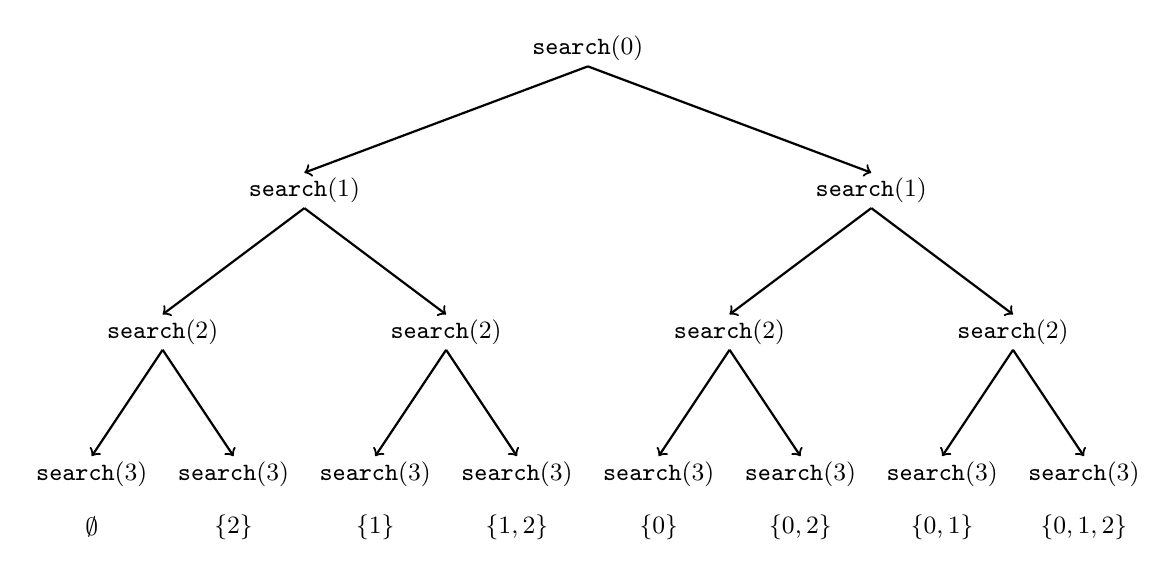
\begin{tikzpicture}[scale=.45]
  \begin{scope}
    \small
    \node at (0,0) {$\texttt{search}(0)$};

    \node at (-8,-4) {$\texttt{search}(1)$};
    \node at (8,-4) {$\texttt{search}(1)$};

    \path[draw,thick,->] (0,0-0.5) -- (-8,-4+0.5);
    \path[draw,thick,->] (0,0-0.5) -- (8,-4+0.5);

    \node at (-12,-8) {$\texttt{search}(2)$};
    \node at (-4,-8) {$\texttt{search}(2)$};
    \node at (4,-8) {$\texttt{search}(2)$};
    \node at (12,-8) {$\texttt{search}(2)$};

    \path[draw,thick,->] (-8,-4-0.5) -- (-12,-8+0.5);
    \path[draw,thick,->] (-8,-4-0.5) -- (-4,-8+0.5);
    \path[draw,thick,->] (8,-4-0.5) -- (4,-8+0.5);
    \path[draw,thick,->] (8,-4-0.5) -- (12,-8+0.5);

    \node at (-14,-12) {$\texttt{search}(3)$};
    \node at (-10,-12) {$\texttt{search}(3)$};
    \node at (-6,-12) {$\texttt{search}(3)$};
    \node at (-2,-12) {$\texttt{search}(3)$};
    \node at (2,-12) {$\texttt{search}(3)$};
    \node at (6,-12) {$\texttt{search}(3)$};
    \node at (10,-12) {$\texttt{search}(3)$};
    \node at (14,-12) {$\texttt{search}(3)$};

    \node at (-14,-13.5) {$\emptyset$};
    \node at (-10,-13.5) {$\{2\}$};
    \node at (-6,-13.5) {$\{1\}$};
    \node at (-2,-13.5) {$\{1,2\}$};
    \node at (2,-13.5) {$\{0\}$};
    \node at (6,-13.5) {$\{0,2\}$};
    \node at (10,-13.5) {$\{0,1\}$};
    \node at (14,-13.5) {$\{0,1,2\}$};


    \path[draw,thick,->] (-12,-8-0.5) -- (-14,-12+0.5);
    \path[draw,thick,->] (-12,-8-0.5) -- (-10,-12+0.5);
    \path[draw,thick,->] (-4,-8-0.5) -- (-6,-12+0.5);
    \path[draw,thick,->] (-4,-8-0.5) -- (-2,-12+0.5);
    \path[draw,thick,->] (4,-8-0.5) -- (2,-12+0.5);
    \path[draw,thick,->] (4,-8-0.5) -- (6,-12+0.5);
    \path[draw,thick,->] (12,-8-0.5) -- (10,-12+0.5);
    \path[draw,thick,->] (12,-8-0.5) -- (14,-12+0.5);
\end{scope}
\end{tikzpicture}
\end{center}

\subsubsection{方法2}

另一种生成子集的方法基于
整数的位表示。
一个包含$n$个元素的集合的每个子集
都可以表示为一个$n$位的序列，
对应于$0 \ldots 2^n-1$之间的一个整数。
位序列中的1表示
哪些元素包含在子集中。

通常的约定是，
最后一位对应元素0，
倒数第二位对应元素1，
以此类推。
例如，25的位表示
是11001，对应子集$\{0,3,4\}$。

以下代码遍历包含$n$个元素的集合的
所有子集

\begin{lstlisting}
for (int b = 0; b < (1<<n); b++) {
    // 处理子集
}
\end{lstlisting}

以下代码展示了如何找出
与某个位序列对应的子集的元素。
在处理每个子集时，
代码构建一个包含该子集中
元素的向量。

\begin{lstlisting}
for (int b = 0; b < (1<<n); b++) {
    vector<int> subset;
    for (int i = 0; i < n; i++) {
        if (b&(1<<i)) subset.push_back(i);
    }
}
\end{lstlisting}

\section{生成排列}

\index{排列}

接下来我们考虑生成一个包含$n$个元素的集合的
所有排列的问题。
例如，$\{0,1,2\}$的排列有
$(0,1,2)$、$(0,2,1)$、$(1,0,2)$、$(1,2,0)$、
$(2,0,1)$和$(2,1,0)$。
同样有两种方法：
我们可以使用递归，也可以
迭代地遍历排列。

\subsubsection{方法1}

与子集类似，排列也可以使用递归来生成。
以下函数\texttt{search}遍历集合$\{0,1,\ldots,n-1\}$的所有排列。
该函数构建一个向量\texttt{permutation}
来存储排列，
当函数不带参数调用时搜索开始。

\begin{lstlisting}
void search() {
    if (permutation.size() == n) {
        // 处理排列
    } else {
        for (int i = 0; i < n; i++) {
            if (chosen[i]) continue;
            chosen[i] = true;
            permutation.push_back(i);
            search();
            chosen[i] = false;
            permutation.pop_back();
        }
    }
}
\end{lstlisting}

每次函数调用都会向\texttt{permutation}
中添加一个新元素。
数组\texttt{chosen}指示哪些
元素已经包含在排列中。
如果\texttt{permutation}的大小等于集合的大小，
则一个排列已经生成。

\subsubsection{方法2}

\index{next\_permutation@\texttt{next\_permutation}}

另一种生成排列的方法是
从排列$\{0,1,\ldots,n-1\}$开始，
重复使用一个函数来构造递增顺序的
下一个排列。
C++标准库中包含函数
\texttt{next\_permutation}，可以用于此目的：

\begin{lstlisting}
vector<int> permutation;
for (int i = 0; i < n; i++) {
    permutation.push_back(i);
}
do {
    // 处理排列
} while (next_permutation(permutation.begin(),permutation.end()));
\end{lstlisting}

\section{回溯}

\index{回溯}

\key{回溯}算法
从一个空解开始，
逐步扩展解。
搜索过程递归地遍历
构造解的所有不同方式。

\index{皇后问题}

作为一个例子，考虑计算在$n \times n$棋盘上放置$n$个皇后
使得没有两个皇后互相攻击的
方法数量的问题。
例如，当$n=4$时，
有两个可能的解：

\begin{center}
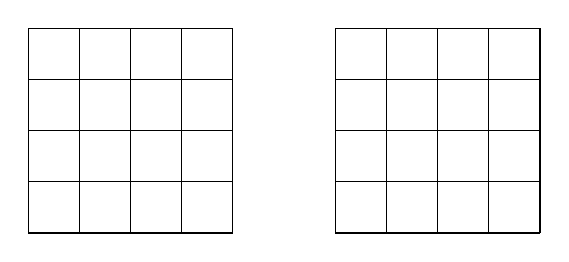
\begin{tikzpicture}[scale=.65]
  \begin{scope}
    \draw (0, 0) grid (4, 4);
    \node at (1.5,3.5) {\symqueen};
    \node at (3.5,2.5) {\symqueen};
    \node at (0.5,1.5) {\symqueen};
    \node at (2.5,0.5) {\symqueen};

    \draw (6, 0) grid (10, 4);
    \node at (6+2.5,3.5) {\symqueen};
    \node at (6+0.5,2.5) {\symqueen};
    \node at (6+3.5,1.5) {\symqueen};
    \node at (6+1.5,0.5) {\symqueen};

  \end{scope}
\end{tikzpicture}
\end{center}

这个问题可以用回溯法解决，
方法是逐行将皇后放置到棋盘上。
更准确地说，每一行恰好放置
一个皇后，使得没有皇后攻击
之前放置的任何皇后。
当所有$n$个皇后都放置到棋盘上时，
就找到了一个解。

例如，当$n=4$时，
回溯算法生成的一些部分解如下：

\begin{center}
\begin{tikzpicture}[scale=.55]
  \begin{scope}
    \draw (0, 0) grid (4, 4);

    \draw (-9, -6) grid (-5, -2);
    \draw (-3, -6) grid (1, -2);
    \draw (3, -6) grid (7, -2);
    \draw (9, -6) grid (13, -2);

    \node at (-9+0.5,-3+0.5) {\symqueen};
    \node at (-3+1+0.5,-3+0.5) {\symqueen};
    \node at (3+2+0.5,-3+0.5) {\symqueen};
    \node at (9+3+0.5,-3+0.5) {\symqueen};

    \draw (2,0) -- (-7,-2);
    \draw (2,0) -- (-1,-2);
    \draw (2,0) -- (5,-2);
    \draw (2,0) -- (11,-2);

    \draw (-11, -12) grid (-7, -8);
    \draw (-6, -12) grid (-2, -8);
    \draw (-1, -12) grid (3, -8);
    \draw (4, -12) grid (8, -8);
    \draw[white] (11, -12) grid (15, -8);
    \node at (-11+1+0.5,-9+0.5) {\symqueen};
    \node at (-6+1+0.5,-9+0.5) {\symqueen};
    \node at (-1+1+0.5,-9+0.5) {\symqueen};
    \node at (4+1+0.5,-9+0.5) {\symqueen};
    \node at (-11+0+0.5,-10+0.5) {\symqueen};
    \node at (-6+1+0.5,-10+0.5) {\symqueen};
    \node at (-1+2+0.5,-10+0.5) {\symqueen};
    \node at (4+3+0.5,-10+0.5) {\symqueen};

    \draw (-1,-6) -- (-9,-8);
    \draw (-1,-6) -- (-4,-8);
    \draw (-1,-6) -- (1,-8);
    \draw (-1,-6) -- (6,-8);

    \node at (-9,-13) {非法};
    \node at (-4,-13) {非法};
    \node at (1,-13) {非法};
    \node at (6,-13) {合法};

  \end{scope}
\end{tikzpicture}
\end{center}

在最底层，前三个配置
是非法的，因为皇后之间互相攻击。
然而，第四个配置是合法的，
通过再放置两个皇后到棋盘上，
它可以扩展为一个完整的解。
只有一种方法来放置剩余的两个皇后。

\begin{samepage}
该算法可以按如下方式实现：
\begin{lstlisting}
void search(int y) {
    if (y == n) {
        count++;
        return;
    }
    for (int x = 0; x < n; x++) {
        if (column[x] || diag1[x+y] || diag2[x-y+n-1]) continue;
        column[x] = diag1[x+y] = diag2[x-y+n-1] = 1;
        search(y+1);
        column[x] = diag1[x+y] = diag2[x-y+n-1] = 0;
    }
}
\end{lstlisting}
\end{samepage}
搜索从调用\texttt{search(0)}开始。
棋盘的大小为$n \times n$，
代码将解的数量计算到
\texttt{count}中。

代码假设棋盘的行和列
从0编号到$n-1$。
当函数\texttt{search}
以参数$y$调用时，
它在第$y$行放置一个皇后，
然后以参数$y+1$调用自身。
如果$y=n$，则找到一个解，
变量\texttt{count}增加一。

数组\texttt{column}记录包含皇后的列，
数组\texttt{diag1}和\texttt{diag2}
记录对角线。
不允许向已经包含皇后的列或对角线上
再添加另一个皇后。
例如，$4 \times 4$棋盘的列和对角线的
编号如下：

\begin{center}
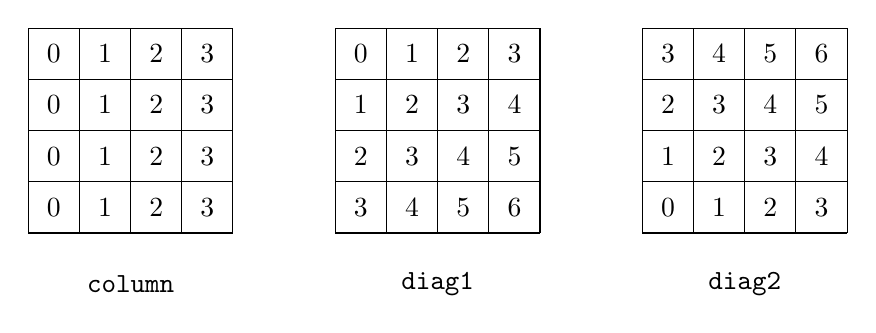
\begin{tikzpicture}[scale=.65]
  \begin{scope}
    \draw (0-6, 0) grid (4-6, 4);
    \node at (-6+0.5,3.5) {$0$};
    \node at (-6+1.5,3.5) {$1$};
    \node at (-6+2.5,3.5) {$2$};
    \node at (-6+3.5,3.5) {$3$};
    \node at (-6+0.5,2.5) {$0$};
    \node at (-6+1.5,2.5) {$1$};
    \node at (-6+2.5,2.5) {$2$};
    \node at (-6+3.5,2.5) {$3$};
    \node at (-6+0.5,1.5) {$0$};
    \node at (-6+1.5,1.5) {$1$};
    \node at (-6+2.5,1.5) {$2$};
    \node at (-6+3.5,1.5) {$3$};
    \node at (-6+0.5,0.5) {$0$};
    \node at (-6+1.5,0.5) {$1$};
    \node at (-6+2.5,0.5) {$2$};
    \node at (-6+3.5,0.5) {$3$};

    \draw (0, 0) grid (4, 4);
    \node at (0.5,3.5) {$0$};
    \node at (1.5,3.5) {$1$};
    \node at (2.5,3.5) {$2$};
    \node at (3.5,3.5) {$3$};
    \node at (0.5,2.5) {$1$};
    \node at (1.5,2.5) {$2$};
    \node at (2.5,2.5) {$3$};
    \node at (3.5,2.5) {$4$};
    \node at (0.5,1.5) {$2$};
    \node at (1.5,1.5) {$3$};
    \node at (2.5,1.5) {$4$};
    \node at (3.5,1.5) {$5$};
    \node at (0.5,0.5) {$3$};
    \node at (1.5,0.5) {$4$};
    \node at (2.5,0.5) {$5$};
    \node at (3.5,0.5) {$6$};

    \draw (6, 0) grid (10, 4);
    \node at (6.5,3.5) {$3$};
    \node at (7.5,3.5) {$4$};
    \node at (8.5,3.5) {$5$};
    \node at (9.5,3.5) {$6$};
    \node at (6.5,2.5) {$2$};
    \node at (7.5,2.5) {$3$};
    \node at (8.5,2.5) {$4$};
    \node at (9.5,2.5) {$5$};
    \node at (6.5,1.5) {$1$};
    \node at (7.5,1.5) {$2$};
    \node at (8.5,1.5) {$3$};
    \node at (9.5,1.5) {$4$};
    \node at (6.5,0.5) {$0$};
    \node at (7.5,0.5) {$1$};
    \node at (8.5,0.5) {$2$};
    \node at (9.5,0.5) {$3$};

    \node at (-4,-1) {\texttt{column}};
    \node at (2,-1) {\texttt{diag1}};
    \node at (8,-1) {\texttt{diag2}};

  \end{scope}
\end{tikzpicture}
\end{center}

令$q(n)$表示在$n \times n$棋盘上
放置$n$个皇后的方法数量。
上述回溯算法告诉我们，
例如$q(8)=92$。
当$n$增大时，搜索很快变慢，
因为解的数量呈指数级增长。
例如，使用上述算法计算$q(16)=14772512$
在现代计算机上已经大约需要一分钟\footnote{目前没有已知的方法可以高效地
计算更大的$q(n)$值。当前记录是
$q(27)=234907967154122528$，于2016年计算得出 \cite{q27}。}。

\section{搜索剪枝}

我们通常可以通过对搜索树剪枝来
优化回溯算法。
其思想是为算法添加“智能”，
使其尽快发现
一个部分解是否无法扩展
为完整的解。
这种优化可以对搜索效率
产生巨大的影响。

让我们考虑一个问题：
计算在$n \times n$网格中从左上角
到右下角且每个方格恰好访问一次的
路径数量。
例如，在$7 \times 7$网格中，
有111712条这样的路径。
其中一条路径如下：

\begin{center}
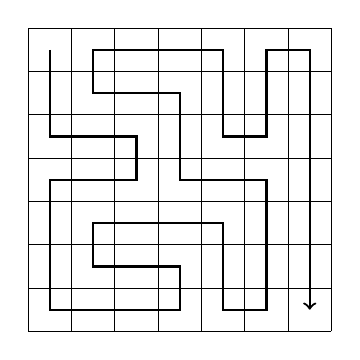
\begin{tikzpicture}[scale=.55]
  \begin{scope}
    \draw (0, 0) grid (7, 7);
    \draw[thick,->] (0.5,6.5) -- (0.5,4.5) -- (2.5,4.5) --
          (2.5,3.5) -- (0.5,3.5) -- (0.5,0.5) --
          (3.5,0.5) -- (3.5,1.5) -- (1.5,1.5) --
          (1.5,2.5) -- (4.5,2.5) -- (4.5,0.5) --
          (5.5,0.5) -- (5.5,3.5) -- (3.5,3.5) --
          (3.5,5.5) -- (1.5,5.5) -- (1.5,6.5) --
          (4.5,6.5) -- (4.5,4.5) -- (5.5,4.5) --
          (5.5,6.5) -- (6.5,6.5) -- (6.5,0.5);
  \end{scope}
\end{tikzpicture}
\end{center}

我们重点关注$7 \times 7$的情况，
因为其难度级别适合我们的需要。
我们从一个简单的回溯算法开始，
然后通过观察如何剪枝搜索
来逐步优化它。
在每次优化之后，我们测量算法的运行时间
和递归调用的次数，
以便清楚地看到每次优化
对搜索效率的影响。

\subsubsection{基本算法}

算法的第一个版本不包含
任何优化。我们简单地使用回溯来生成
从左上角到右下角的所有可能路径，
并统计这样的路径数量。

\begin{itemize}
\item
运行时间：483秒
\item
递归调用次数：760亿次
\end{itemize}

\subsubsection{优化1}

在任何解中，我们首先向下或向右
移动一步。
在第一步之后，总是有两条路径
关于网格的对角线对称。
例如，以下路径是对称的：

\begin{center}
\begin{tabular}{ccc}
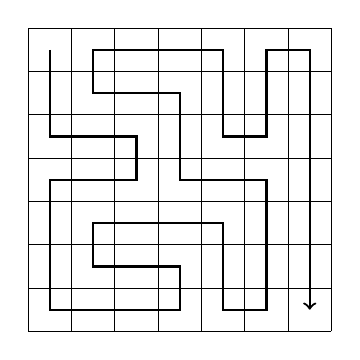
\begin{tikzpicture}[scale=.55]
  \begin{scope}
    \draw (0, 0) grid (7, 7);
    \draw[thick,->] (0.5,6.5) -- (0.5,4.5) -- (2.5,4.5) --
          (2.5,3.5) -- (0.5,3.5) -- (0.5,0.5) --
          (3.5,0.5) -- (3.5,1.5) -- (1.5,1.5) --
          (1.5,2.5) -- (4.5,2.5) -- (4.5,0.5) --
          (5.5,0.5) -- (5.5,3.5) -- (3.5,3.5) --
          (3.5,5.5) -- (1.5,5.5) -- (1.5,6.5) --
          (4.5,6.5) -- (4.5,4.5) -- (5.5,4.5) --
          (5.5,6.5) -- (6.5,6.5) -- (6.5,0.5);
  \end{scope}
\end{tikzpicture}
& \hspace{20pt}
& 
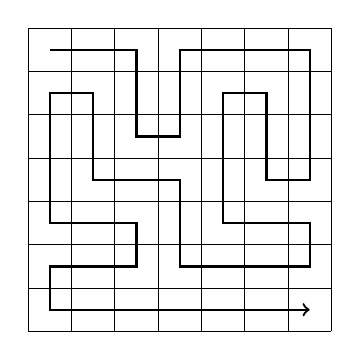
\begin{tikzpicture}[scale=.55]
  \begin{scope}[yscale=1,xscale=-1,rotate=-90]
    \draw (0, 0) grid (7, 7);
    \draw[thick,->] (0.5,6.5) -- (0.5,4.5) -- (2.5,4.5) --
          (2.5,3.5) -- (0.5,3.5) -- (0.5,0.5) --
          (3.5,0.5) -- (3.5,1.5) -- (1.5,1.5) --
          (1.5,2.5) -- (4.5,2.5) -- (4.5,0.5) --
          (5.5,0.5) -- (5.5,3.5) -- (3.5,3.5) --
          (3.5,5.5) -- (1.5,5.5) -- (1.5,6.5) --
          (4.5,6.5) -- (4.5,4.5) -- (5.5,4.5) --
          (5.5,6.5) -- (6.5,6.5) -- (6.5,0.5);
  \end{scope}
\end{tikzpicture}
\end{tabular}
\end{center}

因此，我们可以决定总是先
向下（或向右）移动一步，
最后将解的数量乘以二。

\begin{itemize}
\item
运行时间：244秒
\item
递归调用次数：380亿次
\end{itemize}

\subsubsection{优化2}

如果路径在访问网格中所有其他方格之前
就到达了右下角的方格，
显然不可能完成这个解。
以下路径就是一个例子：

\begin{center}
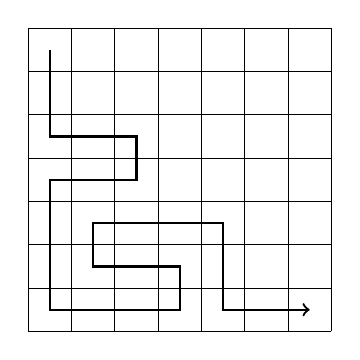
\begin{tikzpicture}[scale=.55]
  \begin{scope}
    \draw (0, 0) grid (7, 7);
    \draw[thick,->] (0.5,6.5) -- (0.5,4.5) -- (2.5,4.5) --
          (2.5,3.5) -- (0.5,3.5) -- (0.5,0.5) --
          (3.5,0.5) -- (3.5,1.5) -- (1.5,1.5) --
          (1.5,2.5) -- (4.5,2.5) -- (4.5,0.5) --
          (6.5,0.5);
  \end{scope}
\end{tikzpicture}
\end{center}
利用这个观察，如果过早到达右下角的方格，
我们可以立即终止搜索。
\begin{itemize}
\item
运行时间：119秒
\item
递归调用次数：200亿次
\end{itemize}

\subsubsection{优化3}

如果路径碰到墙壁，
并且可以向左或向右转，
则网格被分割成两个
包含未访问方格的部分。
例如，在以下情况中，
路径可以向左或向右转：

\begin{center}
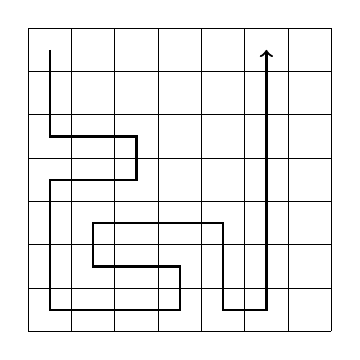
\begin{tikzpicture}[scale=.55]
  \begin{scope}
    \draw (0, 0) grid (7, 7);
    \draw[thick,->] (0.5,6.5) -- (0.5,4.5) -- (2.5,4.5) --
          (2.5,3.5) -- (0.5,3.5) -- (0.5,0.5) --
          (3.5,0.5) -- (3.5,1.5) -- (1.5,1.5) --
          (1.5,2.5) -- (4.5,2.5) -- (4.5,0.5) --
          (5.5,0.5) -- (5.5,6.5);
  \end{scope}
\end{tikzpicture}
\end{center}
在这种情况下，我们已经无法访问所有方格，
因此可以终止搜索。
这个优化非常有用：

\begin{itemize}
\item
运行时间：1.8秒
\item
递归调用次数：2.21亿次
\end{itemize}

\subsubsection{优化4}

优化3的思想
可以推广：
如果路径无法继续向前
但可以向左或向右转，
则网格被分割成两个
都包含未访问方格的部分。
例如，考虑以下路径：

\begin{center}
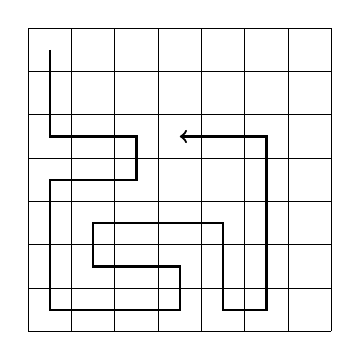
\begin{tikzpicture}[scale=.55]
  \begin{scope}
    \draw (0, 0) grid (7, 7);
    \draw[thick,->] (0.5,6.5) -- (0.5,4.5) -- (2.5,4.5) --
          (2.5,3.5) -- (0.5,3.5) -- (0.5,0.5) --
          (3.5,0.5) -- (3.5,1.5) -- (1.5,1.5) --
          (1.5,2.5) -- (4.5,2.5) -- (4.5,0.5) --
          (5.5,0.5) -- (5.5,4.5) -- (3.5,4.5);
  \end{scope}
\end{tikzpicture}
\end{center}
显然我们已经无法访问所有方格，
因此可以终止搜索。
经过这次优化后，搜索变得
非常高效：

\begin{itemize}
\item
运行时间：0.6秒
\item
递归调用次数：6900万次
\end{itemize}

~\\
现在是停止优化算法并
看看我们取得了什么成果的好时机。
原始算法的运行时间
为483秒，
而经过优化后，
运行时间仅为0.6秒。
因此，算法经过优化后
快了近1000倍。

这是回溯中的常见现象，
因为搜索树通常很大，
即使是简单的观察也能有效地
剪枝搜索。
特别是在算法的最初几步
（即搜索树的顶部）发生的优化
尤其有用。

\section{折半搜索}

\index{折半搜索}

\key{折半搜索}（Meet in the middle）是一种
将搜索空间分成
大小大致相等的两部分的
技术。
对两部分分别进行搜索，
最后将搜索结果合并。

如果有高效的方法可以合并
搜索结果，
则可以使用该技术。
在这种情况下，两次搜索可能
比一次大搜索所需的时间更少。
通常，使用折半搜索技术
可以将$2^n$的因子
转化为$2^{n/2}$的因子。

作为一个例子，考虑这样一个问题：
给定一个包含$n$个数的列表和
一个数$x$，
我们想找出是否可以从列表中选择一些数
使得它们的和为$x$。
例如，给定列表$[2,4,5,9]$和$x=15$，
我们可以选择数字$[2,4,9]$，因为$2+4+9=15$。
然而，如果对同一个列表$x=10$，
则不可能组成该和。

解决这个问题的一个简单算法是
遍历所有元素子集，
检查是否有任何子集的和为$x$。
这种算法的运行时间为$O(2^n)$，
因为有$2^n$个子集。
然而，使用折半搜索技术，
我们可以实现更高效的$O(2^{n/2})$时间算法\footnote{这个
思想由 E. Horowitz 和 S. Sahni 于1974年提出 \cite{hor74}。}。
注意，$O(2^n)$和$O(2^{n/2})$
是不同的复杂度，因为$2^{n/2}$等于$\sqrt{2^n}$。

其思想是将列表分成
两个列表$A$和$B$，使得两个
列表各包含大约一半的数。
第一次搜索生成$A$的所有子集，
并将其和存储到列表$S_A$中。
相应地，第二次搜索从$B$创建
列表$S_B$。
之后，只需检查是否可以从$S_A$中选择一个元素
以及从$S_B$中选择另一个元素，
使得它们的和为$x$。
当且仅当有一种方法可以使用原始列表中的数
组成和$x$时，这是可能的。

例如，假设列表为$[2,4,5,9]$且$x=15$。
首先，我们将列表分为$A=[2,4]$和$B=[5,9]$。
之后，我们创建列表
$S_A=[0,2,4,6]$和$S_B=[0,5,9,14]$。
在这种情况下，和$x=15$是可以组成的，
因为$S_A$包含和$6$，
$S_B$包含和$9$，且$6+9=15$。
这对应于解$[2,4,9]$。

我们可以这样实现算法，
使其时间复杂度为$O(2^{n/2})$。
首先，我们生成\emph{有序的}列表$S_A$和$S_B$，
这可以在$O(2^{n/2})$时间内使用类似归并的技术完成。
之后，由于列表是有序的，
我们可以在$O(2^{n/2})$时间内检查
是否可以从$S_A$和$S_B$创建和$x$。
\chapter{贪心算法}

\index{贪心算法}

\key{贪心算法}通过在每一步
选择当前看起来最优的方案
来构造问题的解。
贪心算法不会撤回已做出的选择，
而是直接构造最终解。
因此，贪心算法通常非常高效。

设计贪心算法的难点在于找到一个
贪心策略，使得该策略总能产生
问题的最优解。
贪心算法中的局部最优选择
也应该是全局最优的。
要论证一个贪心算法的正确性
通常是困难的。

\section{硬币问题}

作为第一个例子，我们考虑这样一个问题：
给定一组硬币，
我们的任务是使用这些硬币
凑出一个金额 $n$。
硬币的面值为
$\texttt{coins}=\{c_1,c_2,\ldots,c_k\}$，
每种硬币可以无限次使用。
最少需要多少枚硬币？

例如，如果硬币是欧元硬币（单位：分）
\[\{1,2,5,10,20,50,100,200\}\]
且 $n=520$，
我们至少需要四枚硬币。
最优解是选择硬币
$200+200+100+20$，其总和为 520。

\subsubsection{贪心算法}

一个简单的贪心算法
总是选择尽可能大的硬币，
直到凑出所需的金额。
这个算法在示例情况下是有效的，
因为我们首先选择两枚 200 分的硬币，
然后选择一枚 100 分的硬币，
最后选择一枚 20 分的硬币。
但这个算法是否总是有效呢？

事实证明，如果硬币是欧元硬币，
贪心算法\emph{总是}有效的，也就是说，
它总是产生一个使用最少硬币数的解。
该算法的正确性可以
通过以下方式证明：

首先，硬币 1、5、10、50 和 100
在最优解中最多出现一次，
因为如果解中包含两枚这样的硬币，
我们可以用一枚硬币替换它们
从而得到更好的解。
例如，如果解中包含硬币 $5+5$，
我们可以用硬币 $10$ 替换它们。

同样地，硬币 2 和 20
在最优解中最多出现两次，
因为我们可以将
硬币 $2+2+2$ 替换为硬币 $5+1$，
将硬币 $20+20+20$ 替换为硬币 $50+10$。
此外，最优解不可能包含
硬币 $2+2+1$ 或 $20+20+10$，
因为我们可以将它们分别替换为硬币 $5$ 和 $50$。

利用这些观察结果，
我们可以对每个硬币 $x$ 证明：
仅使用比 $x$ 小的硬币，
不可能最优地凑出
$x$ 或更大的金额。
例如，如果 $x=100$，使用较小的硬币
能凑出的最大最优和是 $50+20+20+5+2+2=99$。
因此，总是选择最大硬币的贪心算法
产生最优解。

这个例子说明，即使算法本身很简单，
要论证贪心算法的正确性
也可能是困难的。

\subsubsection{一般情况}

在一般情况下，硬币集合可以包含任意硬币，
贪心算法\emph{不一定}能产生
最优解。

我们可以通过给出一个反例
（即算法给出错误答案的情况）
来证明某个贪心算法不正确。
在这个问题中，我们可以很容易地找到一个反例：
如果硬币为 $\{1,3,4\}$ 且目标金额
为 6，贪心算法产生的解为
$4+1+1$，而最优解为 $3+3$。

目前尚不知道一般的硬币问题
是否可以用任何贪心算法来解决\footnote{然而，可以在多项式时间内\emph{检验}
本章中给出的贪心算法对于给定的硬币集合是否有效 \cite{pea05}。}。
但是，正如我们在第 7 章中将看到的，
在某些情况下，
一般问题可以
使用动态规划算法高效求解，
该算法总能给出正确的答案。

\section{调度}

许多调度问题可以用贪心算法来解决。
一个经典问题如下：
给定 $n$ 个事件及其开始时间和结束时间，
找到一个能包含尽可能多事件的安排方案。
不能部分地选择一个事件。
例如，考虑以下事件：
\begin{center}
\begin{tabular}{lll}
事件 & 开始时间 & 结束时间 \\
\hline
$A$ & 1 & 3 \\
$B$ & 2 & 5 \\
$C$ & 3 & 9 \\
$D$ & 6 & 8 \\
\end{tabular}
\end{center}
在这种情况下，最多可以选择两个事件。
例如，我们可以选择事件 $B$ 和 $D$，
如下所示：
\begin{center}
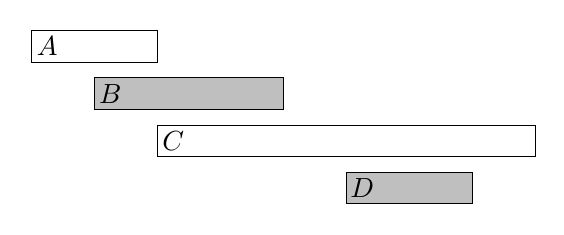
\begin{tikzpicture}[scale=.4]
  \begin{scope}
    \draw (2, 0) rectangle (6, -1);
    \draw[fill=lightgray] (4, -1.5) rectangle (10, -2.5);
    \draw (6, -3) rectangle (18, -4);
    \draw[fill=lightgray] (12, -4.5) rectangle (16, -5.5);
    \node at (2.5,-0.5) {$A$};
    \node at (4.5,-2) {$B$};
    \node at (6.5,-3.5) {$C$};
    \node at (12.5,-5) {$D$};
  \end{scope}
\end{tikzpicture}
\end{center}

对于这个问题，可以想到多种贪心算法，
但哪些算法在所有情况下都有效呢？

\subsubsection*{算法 1}

第一个想法是尽可能选择\emph{短的}
事件。
在示例情况下，这个算法
选择以下事件：
\begin{center}
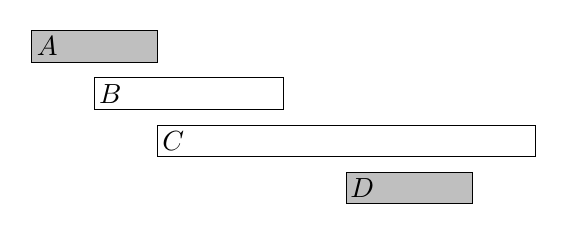
\begin{tikzpicture}[scale=.4]
  \begin{scope}
    \draw[fill=lightgray] (2, 0) rectangle (6, -1);
    \draw (4, -1.5) rectangle (10, -2.5);
    \draw (6, -3) rectangle (18, -4);
    \draw[fill=lightgray] (12, -4.5) rectangle (16, -5.5);
    \node at (2.5,-0.5) {$A$};
    \node at (4.5,-2) {$B$};
    \node at (6.5,-3.5) {$C$};
    \node at (12.5,-5) {$D$};
  \end{scope}
\end{tikzpicture}
\end{center}

然而，选择短事件并不总是一个
正确的策略。例如，算法在以下情况中失败：
\begin{center}
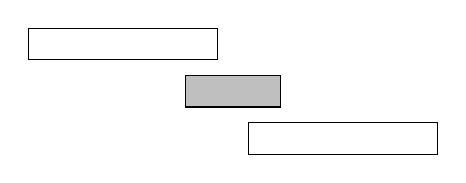
\begin{tikzpicture}[scale=.4]
  \begin{scope}
    \draw (1, 0) rectangle (7, -1);
    \draw[fill=lightgray] (6, -1.5) rectangle (9, -2.5);
    \draw (8, -3) rectangle (14, -4);
  \end{scope}
\end{tikzpicture}
\end{center}
如果我们选择了短事件，就只能选择一个事件。
然而，本来可以选择两个长事件的。

\subsubsection*{算法 2}

另一个想法是总是选择下一个
\emph{开始}尽可能\emph{早}的可用事件。
这个算法选择以下事件：
\begin{center}
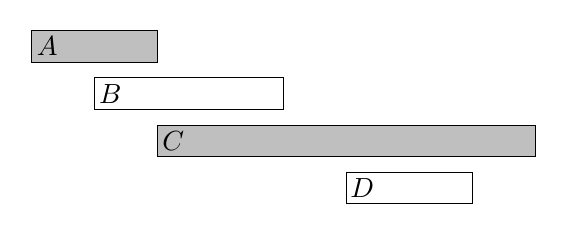
\begin{tikzpicture}[scale=.4]
  \begin{scope}
    \draw[fill=lightgray] (2, 0) rectangle (6, -1);
    \draw (4, -1.5) rectangle (10, -2.5);
    \draw[fill=lightgray] (6, -3) rectangle (18, -4);
    \draw (12, -4.5) rectangle (16, -5.5);
    \node at (2.5,-0.5) {$A$};
    \node at (4.5,-2) {$B$};
    \node at (6.5,-3.5) {$C$};
    \node at (12.5,-5) {$D$};
  \end{scope}
\end{tikzpicture}
\end{center}

然而，我们也可以为这个算法
找到一个反例。
例如，在以下情况中，
算法只选择了一个事件：
\begin{center}
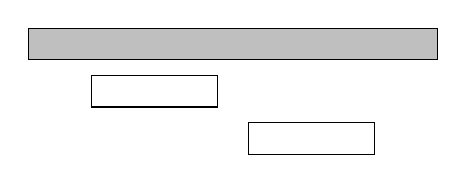
\begin{tikzpicture}[scale=.4]
  \begin{scope}
    \draw[fill=lightgray] (1, 0) rectangle (14, -1);
    \draw (3, -1.5) rectangle (7, -2.5);
    \draw (8, -3) rectangle (12, -4);
  \end{scope}
\end{tikzpicture}
\end{center}
如果我们选择了第一个事件，就无法
再选择任何其他事件。
然而，本来可以选择
另外两个事件的。

\subsubsection*{算法 3}

第三个想法是总是选择下一个
\emph{结束}尽可能\emph{早}的可用事件。
这个算法选择以下事件：
\begin{center}
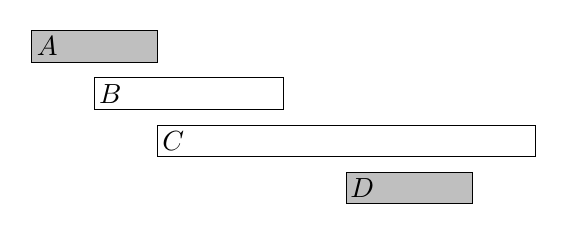
\begin{tikzpicture}[scale=.4]
  \begin{scope}
    \draw[fill=lightgray] (2, 0) rectangle (6, -1);
    \draw (4, -1.5) rectangle (10, -2.5);
    \draw (6, -3) rectangle (18, -4);
    \draw[fill=lightgray] (12, -4.5) rectangle (16, -5.5);
    \node at (2.5,-0.5) {$A$};
    \node at (4.5,-2) {$B$};
    \node at (6.5,-3.5) {$C$};
    \node at (12.5,-5) {$D$};
  \end{scope}
\end{tikzpicture}
\end{center}

事实证明，这个算法
\emph{总是}能产生最优解。
原因是：首先选择一个结束时间尽可能早的事件
总是最优选择。
之后，使用相同的策略选择下一个事件
也是最优选择，以此类推，
直到我们无法再选择更多事件为止。

论证该算法正确性的一种方式是
考虑：如果我们首先选择一个
比最早结束事件结束得更晚的事件，
会发生什么。
此时，我们在选择下一个事件时
最多只能有相同数量的可选方案。
因此，选择一个结束更晚的事件
永远不会产生更好的解，
所以贪心算法是正确的。

\section{任务与截止时间}

现在我们来考虑这样一个问题：
给定 $n$ 个任务，每个任务有其持续时间和截止时间，
我们的任务是选择一个执行任务的顺序。
对于每个任务，我们获得 $d-x$ 分，
其中 $d$ 是任务的截止时间，
$x$ 是我们完成任务的时刻。
我们能获得的最高总分是多少？

例如，假设任务如下：
\begin{center}
\begin{tabular}{lll}
任务 & 持续时间 & 截止时间 \\
\hline
$A$ & 4 & 2 \\
$B$ & 3 & 5 \\
$C$ & 2 & 7 \\
$D$ & 4 & 5 \\
\end{tabular}
\end{center}
在这种情况下，任务的一个最优安排方案
如下：
\begin{center}
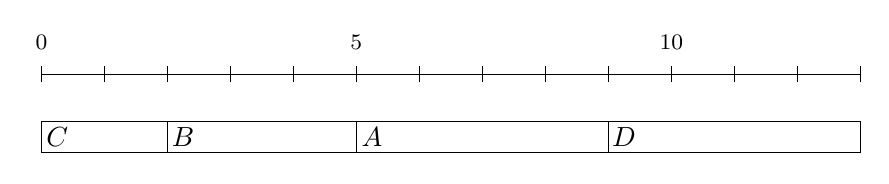
\begin{tikzpicture}[scale=.4]
  \begin{scope}
    \draw (0, 0) rectangle (4, -1);
    \draw (4, 0) rectangle (10, -1);
    \draw (10, 0) rectangle (18, -1);
    \draw (18, 0) rectangle (26, -1);
    \node at (0.5,-0.5) {$C$};
    \node at (4.5,-0.5) {$B$};
    \node at (10.5,-0.5) {$A$};
    \node at (18.5,-0.5) {$D$};

    \draw (0,1.5) -- (26,1.5);
    \foreach \i in {0,2,...,26}
    {
        \draw (\i,1.25) -- (\i,1.75);
    }
    \footnotesize
    \node at (0,2.5) {0};
    \node at (10,2.5) {5};
    \node at (20,2.5) {10};

  \end{scope}
\end{tikzpicture}
\end{center}
在这个方案中，$C$ 获得 5 分，
$B$ 获得 0 分，$A$ 获得 $-7$ 分，
$D$ 获得 $-8$ 分，
所以总分为 $-10$。

令人惊讶的是，这个问题的最优解
完全不依赖于截止时间，
正确的贪心策略仅仅是
将任务\emph{按持续时间排序}，
然后按递增顺序执行。
原因是，如果我们连续执行两个任务，
而第一个任务比第二个任务耗时更长，
那么交换这两个任务可以得到更好的解。
例如，考虑以下安排：
\begin{center}
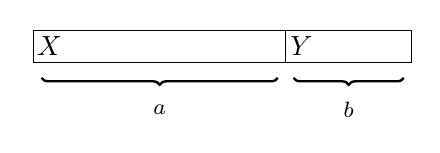
\begin{tikzpicture}[scale=.4]
  \begin{scope}
    \draw (0, 0) rectangle (8, -1);
    \draw (8, 0) rectangle (12, -1);
    \node at (0.5,-0.5) {$X$};
    \node at (8.5,-0.5) {$Y$};

\draw [decoration={brace}, decorate, line width=0.3mm] (7.75,-1.5) -- (0.25,-1.5);
\draw [decoration={brace}, decorate, line width=0.3mm] (11.75,-1.5) -- (8.25,-1.5);

\footnotesize
\node at (4,-2.5) {$a$};
\node at (10,-2.5) {$b$};

  \end{scope}
\end{tikzpicture}
\end{center}
这里 $a>b$，所以我们应该交换任务：
\begin{center}
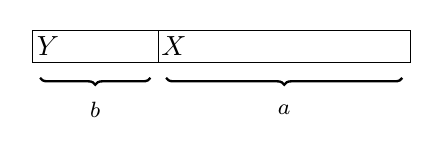
\begin{tikzpicture}[scale=.4]
  \begin{scope}
    \draw (0, 0) rectangle (4, -1);
    \draw (4, 0) rectangle (12, -1);
    \node at (0.5,-0.5) {$Y$};
    \node at (4.5,-0.5) {$X$};

\draw [decoration={brace}, decorate, line width=0.3mm] (3.75,-1.5) -- (0.25,-1.5);
\draw [decoration={brace}, decorate, line width=0.3mm] (11.75,-1.5) -- (4.25,-1.5);

\footnotesize
\node at (2,-2.5) {$b$};
\node at (8,-2.5) {$a$};

  \end{scope}
\end{tikzpicture}
\end{center}
现在 $X$ 少得 $b$ 分，$Y$ 多得 $a$ 分，
所以总分增加了 $a-b > 0$。
在最优解中，对于任意两个连续的任务，
必须保证较短的任务在
较长的任务之前。
因此，任务必须按其持续时间
排序后执行。

\section{最小化和}

接下来我们考虑这样一个问题：
给定 $n$ 个数 $a_1,a_2,\ldots,a_n$，
我们的任务是找到一个值 $x$，
使得以下和最小：
\[|a_1-x|^c+|a_2-x|^c+\cdots+|a_n-x|^c.\]
我们重点关注 $c=1$ 和 $c=2$ 的情况。

\subsubsection{情况 $c=1$}

在这种情况下，我们应该最小化和
\[|a_1-x|+|a_2-x|+\cdots+|a_n-x|.\]
例如，如果这些数是 $[1,2,9,2,6]$，
最好的解是选择 $x=2$，
产生的和为
\[
|1-2|+|2-2|+|9-2|+|2-2|+|6-2|=12.
\]
在一般情况下，$x$ 的最佳选择
是这些数的\textit{中位数}，
即排序后位于中间的数。
例如，列表 $[1,2,9,2,6]$
排序后变为 $[1,2,2,6,9]$，
所以中位数是 2。

中位数是最优选择，
因为如果 $x$ 小于中位数，
增大 $x$ 会使和变小；
如果 $x$ 大于中位数，
减小 $x$ 会使和变小。
因此，最优解是令 $x$
为中位数。
如果 $n$ 是偶数且有两个中位数，
则两个中位数以及它们之间的所有值
都是最优选择。

\subsubsection{情况 $c=2$}

在这种情况下，我们应该最小化和
\[(a_1-x)^2+(a_2-x)^2+\cdots+(a_n-x)^2.\]
例如，如果这些数是 $[1,2,9,2,6]$，
最好的解是选择 $x=4$，
产生的和为
\[
(1-4)^2+(2-4)^2+(9-4)^2+(2-4)^2+(6-4)^2=46.
\]
在一般情况下，$x$ 的最佳选择
是这些数的\emph{平均值}。
在示例中，平均值为 $(1+2+9+2+6)/5=4$。
这个结果可以通过将和表示如下来推导：
\[
nx^2 - 2x(a_1+a_2+\cdots+a_n) + (a_1^2+a_2^2+\cdots+a_n^2)
\]
最后一部分不依赖于 $x$，
所以我们可以忽略它。
剩余部分构成函数
$nx^2-2xs$，其中 $s=a_1+a_2+\cdots+a_n$。
这是一个开口向上的抛物线，
其根为 $x=0$ 和 $x=2s/n$，
最小值为两根的平均值
$x=s/n$，即
数 $a_1,a_2,\ldots,a_n$ 的平均值。

\section{数据压缩}

\index{数据压缩}
\index{二进制码}
\index{码字}

\key{二进制码}为字符串中的每个字符
分配一个由比特组成的\key{码字}。
我们可以使用二进制码\emph{压缩}字符串，
方法是将每个字符替换为
对应的码字。
例如，以下二进制码
为字符 \texttt{A}–\texttt{D} 分配码字：
\begin{center}
\begin{tabular}{rr}
字符 & 码字 \\
\hline
\texttt{A} & 00 \\
\texttt{B} & 01 \\
\texttt{C} & 10 \\
\texttt{D} & 11 \\
\end{tabular}
\end{center}
这是一种\key{定长}码，
意味着每个码字的长度相同。
例如，我们可以将字符串
\texttt{AABACDACA} 压缩如下：
\[00\,00\,01\,00\,10\,11\,00\,10\,00\]
使用这种编码，压缩后的
字符串长度为 18 比特。
然而，如果我们使用\key{变长}码
（其中码字可以有不同的长度），
就可以更好地压缩字符串。
这样我们可以为经常出现的字符
分配较短的码字，
为很少出现的字符
分配较长的码字。
事实证明，上述字符串的一个\key{最优}码
如下：
\begin{center}
\begin{tabular}{rr}
字符 & 码字 \\
\hline
\texttt{A} & 0 \\
\texttt{B} & 110 \\
\texttt{C} & 10 \\
\texttt{D} & 111 \\
\end{tabular}
\end{center}
最优码产生尽可能短的
压缩字符串。
在这种情况下，使用最优码压缩后的
字符串为
\[0\,0\,110\,0\,10\,111\,0\,10\,0,\]
所以只需要 15 比特，而不是 18 比特。
因此，得益于更好的编码，
压缩字符串中节省了 3 比特。

我们要求没有任何码字
是另一个码字的前缀。
例如，不允许一个编码
同时包含码字 10
和 1011。
原因是我们希望能够从压缩字符串
还原出原始字符串。
如果一个码字可以是另一个码字的前缀，
这就不是总能做到的。
例如，以下编码是\emph{无效}的：
\begin{center}
\begin{tabular}{rr}
字符 & 码字 \\
\hline
\texttt{A} & 10 \\
\texttt{B} & 11 \\
\texttt{C} & 1011 \\
\texttt{D} & 111 \\
\end{tabular}
\end{center}
使用这种编码，我们无法确定
压缩字符串 1011 对应的是
字符串 \texttt{AB} 还是字符串 \texttt{C}。

\index{哈夫曼编码}

\subsubsection{哈夫曼编码}

\key{哈夫曼编码}\footnote{D. A. Huffman 在解答一门大学课程的作业时发现了这种方法，
并于 1952 年发表了该算法 \cite{huf52}。}是一种贪心算法，
用于构造压缩给定字符串的
最优编码。
该算法基于字符串中各字符的频率
构建一棵二叉树，
每个字符的码字可以通过
从根节点到对应节点的路径来读取。
向左走对应比特 0，
向右走对应比特 1。

初始时，字符串中的每个字符由一个
节点表示，其权重为该字符
在字符串中出现的次数。
然后在每一步中，选择权重最小的两个节点
进行合并，创建一个新节点，
其权重为原始两个节点权重之和。
这个过程持续进行，直到所有节点都被合并。

接下来我们将看到哈夫曼编码如何
为字符串 \texttt{AABACDACA}
创建最优编码。
初始时，有四个节点分别对应
字符串中的字符：

\begin{center}
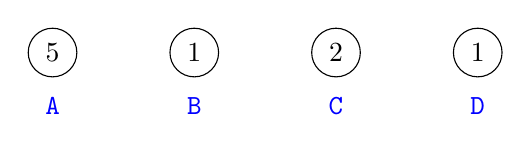
\begin{tikzpicture}[scale=0.9]
\node[draw, circle] (1) at (0,0) {$5$};
\node[draw, circle] (2) at (2,0) {$1$};
\node[draw, circle] (3) at (4,0) {$2$};
\node[draw, circle] (4) at (6,0) {$1$};

\node[color=blue] at (0,-0.75) {\texttt{A}};
\node[color=blue] at (2,-0.75) {\texttt{B}};
\node[color=blue] at (4,-0.75) {\texttt{C}};
\node[color=blue] at (6,-0.75) {\texttt{D}};

%\path[draw,thick,-] (4) -- (5);
\end{tikzpicture}
\end{center}
表示字符 \texttt{A} 的节点
权重为 5，因为字符 \texttt{A}
在字符串中出现了 5 次。
其他权重以相同的方式
计算得到。

第一步是合并对应字符 \texttt{B} 和 \texttt{D}
的节点，两者的权重都是 1。
结果如下：
\begin{center}
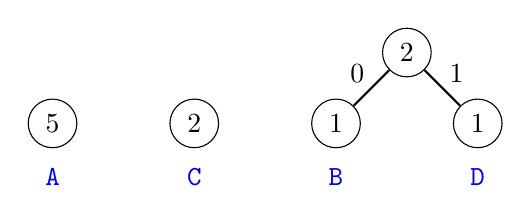
\begin{tikzpicture}[scale=0.9]
\node[draw, circle] (1) at (0,0) {$5$};
\node[draw, circle] (3) at (2,0) {$2$};
\node[draw, circle] (2) at (4,0) {$1$};
\node[draw, circle] (4) at (6,0) {$1$};
\node[draw, circle] (5) at (5,1) {$2$};

\node[color=blue] at (0,-0.75) {\texttt{A}};
\node[color=blue] at (2,-0.75) {\texttt{C}};
\node[color=blue] at (4,-0.75) {\texttt{B}};
\node[color=blue] at (6,-0.75) {\texttt{D}};

\node at (4.3,0.7) {0};
\node at (5.7,0.7) {1};

\path[draw,thick,-] (2) -- (5);
\path[draw,thick,-] (4) -- (5);
\end{tikzpicture}
\end{center}
之后，权重为 2 的节点被合并：
\begin{center}
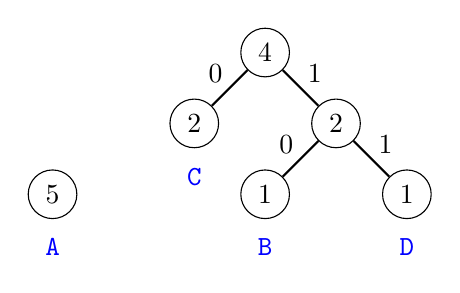
\begin{tikzpicture}[scale=0.9]
\node[draw, circle] (1) at (1,0) {$5$};
\node[draw, circle] (3) at (3,1) {$2$};
\node[draw, circle] (2) at (4,0) {$1$};
\node[draw, circle] (4) at (6,0) {$1$};
\node[draw, circle] (5) at (5,1) {$2$};
\node[draw, circle] (6) at (4,2) {$4$};

\node[color=blue] at (1,-0.75) {\texttt{A}};
\node[color=blue] at (3,1-0.75) {\texttt{C}};
\node[color=blue] at (4,-0.75) {\texttt{B}};
\node[color=blue] at (6,-0.75) {\texttt{D}};

\node at (4.3,0.7) {0};
\node at (5.7,0.7) {1};
\node at (3.3,1.7) {0};
\node at (4.7,1.7) {1};

\path[draw,thick,-] (2) -- (5);
\path[draw,thick,-] (4) -- (5);
\path[draw,thick,-] (3) -- (6);
\path[draw,thick,-] (5) -- (6);
\end{tikzpicture}
\end{center}
最后，合并剩下的两个节点：
\begin{center}
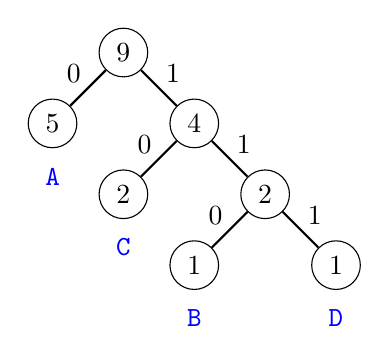
\begin{tikzpicture}[scale=0.9]
\node[draw, circle] (1) at (2,2) {$5$};
\node[draw, circle] (3) at (3,1) {$2$};
\node[draw, circle] (2) at (4,0) {$1$};
\node[draw, circle] (4) at (6,0) {$1$};
\node[draw, circle] (5) at (5,1) {$2$};
\node[draw, circle] (6) at (4,2) {$4$};
\node[draw, circle] (7) at (3,3) {$9$};

\node[color=blue] at (2,2-0.75) {\texttt{A}};
\node[color=blue] at (3,1-0.75) {\texttt{C}};
\node[color=blue] at (4,-0.75) {\texttt{B}};
\node[color=blue] at (6,-0.75) {\texttt{D}};

\node at (4.3,0.7) {0};
\node at (5.7,0.7) {1};
\node at (3.3,1.7) {0};
\node at (4.7,1.7) {1};
\node at (2.3,2.7) {0};
\node at (3.7,2.7) {1};

\path[draw,thick,-] (2) -- (5);
\path[draw,thick,-] (4) -- (5);
\path[draw,thick,-] (3) -- (6);
\path[draw,thick,-] (5) -- (6);
\path[draw,thick,-] (1) -- (7);
\path[draw,thick,-] (6) -- (7);
\end{tikzpicture}
\end{center}

现在所有节点都在树中了，编码已完成。
从树中可以读取以下码字：
\begin{center}
\begin{tabular}{rr}
字符 & 码字 \\
\hline
\texttt{A} & 0 \\
\texttt{B} & 110 \\
\texttt{C} & 10 \\
\texttt{D} & 111 \\
\end{tabular}
\end{center}

\chapter{动态规划}

\index{动态规划}

\key{动态规划}是一种结合了
完备搜索的正确性和
贪心算法的效率的技术。
如果问题可以被分解为
可以独立求解的重叠子问题，
就可以使用动态规划。

动态规划有两种用途：

\begin{itemize}
\item
\key{寻找最优解}：
我们希望找到一个尽可能大
或尽可能小的解。
\item
\key{计算解的数量}：
我们希望计算所有
可能解的总数。
\end{itemize}

我们将首先了解如何使用动态规划
来寻找最优解，
然后再用同样的思想来
计算解的数量。

理解动态规划是每个
竞赛程序员职业生涯中的一个里程碑。
虽然基本思想很简单，
但挑战在于如何将
动态规划应用于不同的问题。
本章介绍了一组经典问题，
它们是一个很好的起点。

\section{硬币问题}

我们首先关注一个
在第6章中已经见过的问题：
给定一组硬币面值 $\texttt{coins} = \{c_1,c_2,\ldots,c_k\}$
和一个目标金额 $n$，
我们的任务是使用尽可能少的硬币
来凑成金额 $n$。

在第6章中，我们使用
贪心算法来解决这个问题，
该算法总是选择尽可能大的硬币。
例如，当硬币是欧元硬币时，
贪心算法是有效的，
但在一般情况下，贪心算法
不一定能产生最优解。

现在是时候使用动态规划
来高效地解决这个问题了，
这样算法就能适用于任何硬币集合。
动态规划算法基于一个递归函数，
该函数遍历所有凑成金额的可能方式，
就像暴力算法一样。
然而，动态规划算法是高效的，
因为它使用了\emph{记忆化}，
并且每个子问题的答案只计算一次。

\subsubsection{递归公式}

动态规划的思想是将
问题用递归的方式表达，
使得问题的解可以
从更小的子问题的解中计算出来。
在硬币问题中，一个自然的递归
问题如下：
凑成金额 $x$ 所需的最少硬币数
是多少？

令 $\texttt{solve}(x)$
表示凑成金额 $x$ 所需的
最少硬币数。
函数的值取决于
硬币的面值。
例如，如果 $\texttt{coins} = \{1,3,4\}$，
函数的前几个值如下：

\[
\begin{array}{lcl}
\texttt{solve}(0) & = & 0 \\
\texttt{solve}(1) & = & 1 \\
\texttt{solve}(2) & = & 2 \\
\texttt{solve}(3) & = & 1 \\
\texttt{solve}(4) & = & 1 \\
\texttt{solve}(5) & = & 2 \\
\texttt{solve}(6) & = & 2 \\
\texttt{solve}(7) & = & 2 \\
\texttt{solve}(8) & = & 2 \\
\texttt{solve}(9) & = & 3 \\
\texttt{solve}(10) & = & 3 \\
\end{array}
\]

例如，$\texttt{solve}(10)=3$，
因为凑成金额10至少需要3枚硬币。
最优解是 $3+3+4=10$。

$\texttt{solve}$ 的关键性质是
它的值可以
从更小的值递归地计算出来。
核心思想是关注我们为金额选择的
\emph{第一枚}硬币。
例如，在上述场景中，
第一枚硬币可以是1、3或4。
如果我们首先选择硬币1，
那么剩下的任务就是用最少的硬币
凑成金额9，
这是原问题的一个子问题。
当然，硬币3和4也是如此。
因此，我们可以使用以下递归公式
来计算最少的硬币数：
\begin{equation*}
\begin{split}
\texttt{solve}(x) = \min( & \texttt{solve}(x-1)+1, \\
                           & \texttt{solve}(x-3)+1, \\
                           & \texttt{solve}(x-4)+1).
\end{split}
\end{equation*}
递归的边界条件是 $\texttt{solve}(0)=0$，
因为凑成空金额不需要任何硬币。
例如，
\[ \texttt{solve}(10) = \texttt{solve}(7)+1 = \texttt{solve}(4)+2 = \texttt{solve}(0)+3 = 3.\]

现在我们准备给出一个通用的递归函数，
计算凑成金额 $x$ 
所需的最少硬币数：
\begin{equation*}
    \texttt{solve}(x) = \begin{cases}
               \infty               & x < 0\\
               0               & x = 0\\
               \min_{c \in \texttt{coins}} \texttt{solve}(x-c)+1 & x > 0 \\
           \end{cases}
\end{equation*}

首先，如果 $x<0$，值为 $\infty$，
因为不可能凑成负的金额。
然后，如果 $x=0$，值为 $0$，
因为凑成空金额不需要任何硬币。
最后，如果 $x>0$，变量 $c$ 遍历
选择金额的第一枚硬币的
所有可能方式。

一旦找到了解决问题的递归函数，
我们就可以直接用C++实现解决方案
（常量 \texttt{INF} 表示无穷大）：

\begin{lstlisting}
int solve(int x) {
    if (x < 0) return INF;
    if (x == 0) return 0;
    int best = INF;
    for (auto c : coins) {
        best = min(best, solve(x-c)+1);
    }
    return best;
}
\end{lstlisting}

然而，这个函数并不高效，
因为构造金额可能
有指数级数量的方式。
不过，接下来我们将看到如何使用
一种称为记忆化的技术
来使函数变得高效。

\subsubsection{使用记忆化}

\index{记忆化}

动态规划的思想是使用
\key{记忆化}来高效地计算
递归函数的值。
这意味着函数的值在计算后
会被存储在数组中。
对于每个参数，函数的值
只会递归计算一次，之后
就可以直接从数组中获取该值。

在这个问题中，我们使用数组
\begin{lstlisting}
bool ready[N];
int value[N];
\end{lstlisting}

其中 $\texttt{ready}[x]$ 表示
$\texttt{solve}(x)$ 的值是否已经被计算过，
如果是，则 $\texttt{value}[x]$
包含这个值。
常量 $N$ 的选择应确保
所有需要的值都能放入数组中。

现在这个函数可以高效地
实现如下：

\begin{lstlisting}
int solve(int x) {
    if (x < 0) return INF;
    if (x == 0) return 0;
    if (ready[x]) return value[x];
    int best = INF;
    for (auto c : coins) {
        best = min(best, solve(x-c)+1);
    }
    value[x] = best;
    ready[x] = true;
    return best;
}
\end{lstlisting}

函数像之前一样处理
边界情况 $x<0$ 和 $x=0$。
然后函数通过
$\texttt{ready}[x]$ 检查
$\texttt{solve}(x)$ 是否已经被存储
在 $\texttt{value}[x]$ 中，
如果是，函数直接返回它。
否则，函数递归地计算
$\texttt{solve}(x)$ 的值
并将其存储在 $\texttt{value}[x]$ 中。

这个函数高效地工作，
因为每个参数 $x$ 的答案
只会被递归计算一次。
在 $\texttt{solve}(x)$ 的值被存储在 $\texttt{value}[x]$ 之后，
每当函数再次以参数 $x$ 被调用时，
就可以高效地获取它。
算法的时间复杂度为 $O(nk)$，
其中 $n$ 是目标金额，$k$ 是硬币的数量。

注意，我们也可以\emph{迭代地}
构造数组 \texttt{value}，
只需使用一个循环计算
$\texttt{solve}$ 在参数 $0 \ldots n$ 上的
所有值：
\begin{lstlisting}
value[0] = 0;
for (int x = 1; x <= n; x++) {
    value[x] = INF;
    for (auto c : coins) {
        if (x-c >= 0) {
            value[x] = min(value[x], value[x-c]+1);
        }
    }
}
\end{lstlisting}

事实上，大多数竞赛程序员更喜欢这种
实现方式，因为它更短而且
常数因子更低。
从现在起，我们在示例中也
使用迭代实现。
尽管如此，用递归函数的方式来思考
动态规划解决方案通常更加容易。


\subsubsection{构造解}

有时我们不仅被要求找到
最优解的值，还被要求给出
如何构造这样一个解的示例。
例如，在硬币问题中，
我们可以声明另一个数组，
为每个金额指出
最优解中的第一枚硬币：
\begin{lstlisting}
int first[N];
\end{lstlisting}
然后，我们可以如下修改算法：
\begin{lstlisting}
value[0] = 0;
for (int x = 1; x <= n; x++) {
    value[x] = INF;
    for (auto c : coins) {
        if (x-c >= 0 && value[x-c]+1 < value[x]) {
            value[x] = value[x-c]+1;
            first[x] = c;
        }
    }
}
\end{lstlisting}
之后，可以使用以下代码
打印出金额 $n$ 的
最优解中出现的硬币：
\begin{lstlisting}
while (n > 0) {
    cout << first[n] << "\n";
    n -= first[n];
}
\end{lstlisting}

\subsubsection{计算解的数量}

现在让我们考虑硬币问题的
另一个版本，我们的任务是
计算用硬币凑成金额 $x$ 的
总方法数。
例如，如果 $\texttt{coins}=\{1,3,4\}$ 且
$x=5$，总共有6种方法：

\begin{multicols}{2}
\begin{itemize}
\item $1+1+1+1+1$
\item $1+1+3$
\item $1+3+1$
\item $3+1+1$
\item $1+4$
\item $4+1$
\end{itemize}
\end{multicols}

同样，我们可以递归地解决该问题。
令 $\texttt{solve}(x)$ 表示
我们能凑成金额 $x$ 的方法数。
例如，如果 $\texttt{coins}=\{1,3,4\}$，
那么 $\texttt{solve}(5)=6$，递归公式为
\begin{equation*}
\begin{split}
\texttt{solve}(x) = & \texttt{solve}(x-1) + \\
                    & \texttt{solve}(x-3) + \\
                    & \texttt{solve}(x-4)  .
\end{split}
\end{equation*}

然后，通用的递归函数如下：
\begin{equation*}
    \texttt{solve}(x) = \begin{cases}
               0               & x < 0\\
               1               & x = 0\\
               \sum_{c \in \texttt{coins}} \texttt{solve}(x-c) & x > 0 \\
           \end{cases}
\end{equation*}

如果 $x<0$，值为0，因为没有解。
如果 $x=0$，值为1，因为凑成空金额
只有一种方法。
否则我们计算所有形如
$\texttt{solve}(x-c)$ 的值的总和，
其中 $c$ 属于 \texttt{coins}。

以下代码构造了一个数组
$\texttt{count}$，使得
$\texttt{count}[x]$ 等于
$\texttt{solve}(x)$ 的值，
其中 $0 \le x \le n$：

\begin{lstlisting}
count[0] = 1;
for (int x = 1; x <= n; x++) {
    for (auto c : coins) {
        if (x-c >= 0) {
            count[x] += count[x-c];
        }
    }
}
\end{lstlisting}

通常解的数量非常大，
以至于不需要计算精确值，
只需给出答案模 $m$ 的结果即可，
例如 $m=10^9+7$。
这可以通过修改代码使得
所有计算都对 $m$ 取模来实现。
在上述代码中，只需在以下行之后
\begin{lstlisting}
        count[x] += count[x-c];
\end{lstlisting}
添加这一行：
\begin{lstlisting}
        count[x] %= m;
\end{lstlisting}

我们已经讨论了动态规划的
所有基本思想。
由于动态规划可以在
许多不同的情况下使用，
我们现在将通过一组问题
来进一步展示
动态规划的可能性。

\section{最长递增子序列}

\index{最长递增子序列}

我们的第一个问题是
在包含 $n$ 个元素的数组中找到
\key{最长递增子序列}。
这是一个从左到右的、最大长度的
数组元素序列，
且序列中的每个元素都大于
前一个元素。
例如，在数组

\begin{center}
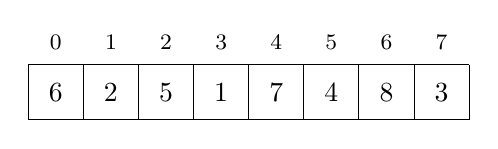
\begin{tikzpicture}[scale=0.7]
\draw (0,0) grid (8,1);
\node at (0.5,0.5) {$6$};
\node at (1.5,0.5) {$2$};
\node at (2.5,0.5) {$5$};
\node at (3.5,0.5) {$1$};
\node at (4.5,0.5) {$7$};
\node at (5.5,0.5) {$4$};
\node at (6.5,0.5) {$8$};
\node at (7.5,0.5) {$3$};

\footnotesize
\node at (0.5,1.4) {$0$};
\node at (1.5,1.4) {$1$};
\node at (2.5,1.4) {$2$};
\node at (3.5,1.4) {$3$};
\node at (4.5,1.4) {$4$};
\node at (5.5,1.4) {$5$};
\node at (6.5,1.4) {$6$};
\node at (7.5,1.4) {$7$};
\end{tikzpicture}
\end{center}
最长递增子序列
包含4个元素：
\begin{center}
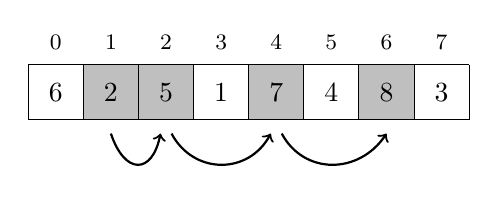
\begin{tikzpicture}[scale=0.7]
\fill[color=lightgray] (1,0) rectangle (2,1);
\fill[color=lightgray] (2,0) rectangle (3,1);
\fill[color=lightgray] (4,0) rectangle (5,1);
\fill[color=lightgray] (6,0) rectangle (7,1);
\draw (0,0) grid (8,1);
\node at (0.5,0.5) {$6$};
\node at (1.5,0.5) {$2$};
\node at (2.5,0.5) {$5$};
\node at (3.5,0.5) {$1$};
\node at (4.5,0.5) {$7$};
\node at (5.5,0.5) {$4$};
\node at (6.5,0.5) {$8$};
\node at (7.5,0.5) {$3$};

\draw[thick,->] (1.5,-0.25) .. controls (1.75,-1.00) and (2.25,-1.00) .. (2.4,-0.25);
\draw[thick,->] (2.6,-0.25) .. controls (3.0,-1.00) and (4.0,-1.00) .. (4.4,-0.25);
\draw[thick,->] (4.6,-0.25) .. controls (5.0,-1.00) and (6.0,-1.00) .. (6.5,-0.25);

\footnotesize
\node at (0.5,1.4) {$0$};
\node at (1.5,1.4) {$1$};
\node at (2.5,1.4) {$2$};
\node at (3.5,1.4) {$3$};
\node at (4.5,1.4) {$4$};
\node at (5.5,1.4) {$5$};
\node at (6.5,1.4) {$6$};
\node at (7.5,1.4) {$7$};
\end{tikzpicture}
\end{center}

令 $\texttt{length}(k)$ 表示
以位置 $k$ 结尾的
最长递增子序列的长度。
因此，如果我们计算
$\texttt{length}(k)$ 在 $0 \le k \le n-1$ 范围内的所有值，
我们就能找到
最长递增子序列的长度。
例如，上述数组对应的
函数值如下：
\[
\begin{array}{lcl}
\texttt{length}(0) & = & 1 \\
\texttt{length}(1) & = & 1 \\
\texttt{length}(2) & = & 2 \\
\texttt{length}(3) & = & 1 \\
\texttt{length}(4) & = & 3 \\
\texttt{length}(5) & = & 2 \\
\texttt{length}(6) & = & 4 \\
\texttt{length}(7) & = & 2 \\
\end{array}
\]

例如，$\texttt{length}(6)=4$，
因为以位置6结尾的最长递增子序列
由4个元素组成。

为了计算 $\texttt{length}(k)$ 的值，
我们需要找到一个位置 $i<k$，
使得 $\texttt{array}[i]<\texttt{array}[k]$
且 $\texttt{length}(i)$ 尽可能大。
然后我们知道
$\texttt{length}(k)=\texttt{length}(i)+1$，
因为这是将 $\texttt{array}[k]$ 
添加到子序列中的最优方式。
然而，如果不存在这样的位置 $i$，
则 $\texttt{length}(k)=1$，
这意味着子序列仅包含
$\texttt{array}[k]$。

由于函数的所有值都可以
从更小的值计算出来，
我们可以使用动态规划。
在以下代码中，函数的值
将被存储在数组
$\texttt{length}$ 中。

\begin{lstlisting}
for (int k = 0; k < n; k++) {
    length[k] = 1;
    for (int i = 0; i < k; i++) {
        if (array[i] < array[k]) {
            length[k] = max(length[k],length[i]+1);
        }
    }
}
\end{lstlisting}

这段代码的时间复杂度为 $O(n^2)$，
因为它由两层嵌套循环组成。
然而，也可以用 $O(n \log n)$ 的时间
更高效地实现
动态规划计算。
你能找到实现方法吗？

\section{网格中的路径}

我们的下一个问题是
在 $n \times n$ 网格中找到一条
从左上角到
右下角的路径，
使得我们只向下和向右移动。
每个格子包含一个正整数，
路径的构造应使
沿路径的值之和尽可能大。

下图展示了一个网格中的
最优路径：
\begin{center}
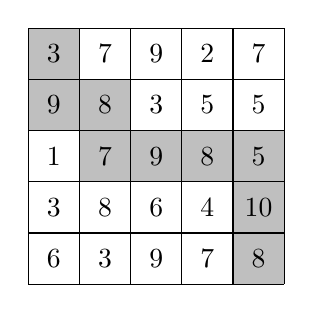
\begin{tikzpicture}[scale=.65]
  \begin{scope}
    \fill [color=lightgray] (0, 9) rectangle (1, 8);
    \fill [color=lightgray] (0, 8) rectangle (1, 7);
    \fill [color=lightgray] (1, 8) rectangle (2, 7);
    \fill [color=lightgray] (1, 7) rectangle (2, 6);
    \fill [color=lightgray] (2, 7) rectangle (3, 6);
    \fill [color=lightgray] (3, 7) rectangle (4, 6);
    \fill [color=lightgray] (4, 7) rectangle (5, 6);
    \fill [color=lightgray] (4, 6) rectangle (5, 5);
    \fill [color=lightgray] (4, 5) rectangle (5, 4);
    \draw (0, 4) grid (5, 9);
    \node at (0.5,8.5) {3};
    \node at (1.5,8.5) {7};
    \node at (2.5,8.5) {9};
    \node at (3.5,8.5) {2};
    \node at (4.5,8.5) {7};
    \node at (0.5,7.5) {9};
    \node at (1.5,7.5) {8};
    \node at (2.5,7.5) {3};
    \node at (3.5,7.5) {5};
    \node at (4.5,7.5) {5};
    \node at (0.5,6.5) {1};
    \node at (1.5,6.5) {7};
    \node at (2.5,6.5) {9};
    \node at (3.5,6.5) {8};
    \node at (4.5,6.5) {5};
    \node at (0.5,5.5) {3};
    \node at (1.5,5.5) {8};
    \node at (2.5,5.5) {6};
    \node at (3.5,5.5) {4};
    \node at (4.5,5.5) {10};
    \node at (0.5,4.5) {6};
    \node at (1.5,4.5) {3};
    \node at (2.5,4.5) {9};
    \node at (3.5,4.5) {7};
    \node at (4.5,4.5) {8};
  \end{scope}
\end{tikzpicture}
\end{center}
路径上值之和为67，
这是从
左上角到右下角的路径上
可能的最大和。

假设网格的行和列
从1到 $n$ 编号，
且 $\texttt{value}[y][x]$ 等于
格子 $(y,x)$ 的值。
令 $\texttt{sum}(y,x)$ 表示
从左上角到格子 $(y,x)$ 的
路径上的最大和。
现在 $\texttt{sum}(n,n)$ 告诉我们
从左上角到
右下角的最大和。
例如，在上述网格中，
$\texttt{sum}(5,5)=67$。

我们可以递归地计算
这些和如下：
\[ \texttt{sum}(y,x) = \max(\texttt{sum}(y,x-1),\texttt{sum}(y-1,x))+\texttt{value}[y][x]\]


递归公式基于这样的观察：
到达格子 $(y,x)$ 的路径
要么来自格子 $(y,x-1)$，
要么来自格子 $(y-1,x)$：
\begin{center}
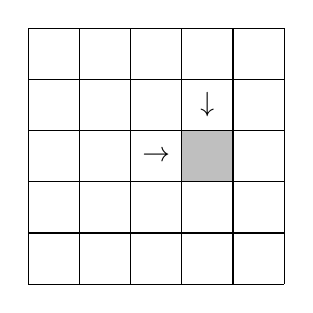
\begin{tikzpicture}[scale=.65]
  \begin{scope}
    \fill [color=lightgray] (3, 7) rectangle (4, 6);
    \draw (0, 4) grid (5, 9);
    
    \node at (2.5,6.5) {$\rightarrow$};
    \node at (3.5,7.5) {$\downarrow$};
    
  \end{scope}
\end{tikzpicture}
\end{center}

因此，我们选择使和
最大化的方向。
我们假设当 $y=0$ 或 $x=0$ 时
$\texttt{sum}(y,x)=0$
（因为这样的路径不存在），
所以递归公式在 $y=1$ 或 $x=1$ 时也适用。

由于函数 \texttt{sum} 有两个参数，
动态规划数组也有两个维度。
例如，我们可以使用数组
\begin{lstlisting}
int sum[N][N];
\end{lstlisting}
并按如下方式计算和：
\begin{lstlisting}
for (int y = 1; y <= n; y++) {
    for (int x = 1; x <= n; x++) {
        sum[y][x] = max(sum[y][x-1],sum[y-1][x])+value[y][x];
    }
}
\end{lstlisting}
算法的时间复杂度为 $O(n^2)$。

\section{背包问题}

\index{背包}

术语\key{背包}指的是这样一类问题：
给定一组物品，
需要找出
具有某些性质的子集。
背包问题通常可以使用
动态规划来解决。

在本节中，我们关注以下问题：
给定一个权重列表
$[w_1,w_2,\ldots,w_n]$，
确定可以使用这些权重
构造的所有和。
例如，如果权重为
$[1,3,3,5]$，以下和是可能的：

\begin{center}
\begin{tabular}{rrrrrrrrrrrrr}
 0 & 1 & 2 & 3 & 4 & 5 & 6 & 7 & 8 & 9 & 10 & 11 & 12 \\
\hline
 X & X & & X & X & X & X & X & X & X & & X & X \\
\end{tabular}
\end{center}

在这种情况下，$0 \ldots 12$ 之间的所有和
都是可能的，除了2和10。
例如，和7是可能的，因为我们
可以选择权重 $[1,3,3]$。

为了解决这个问题，我们关注子问题，
即仅使用前 $k$ 个权重
来构造和。
令 $\texttt{possible}(x,k)=\textrm{true}$ 表示
我们可以用前 $k$ 个权重
构造和 $x$，
否则 $\texttt{possible}(x,k)=\textrm{false}$。
函数的值可以
递归地计算如下：
\[ \texttt{possible}(x,k) = \texttt{possible}(x-w_k,k-1) \lor \texttt{possible}(x,k-1) \]
该公式基于这样一个事实：
我们可以选择使用或不使用
权重 $w_k$ 来构造和。
如果使用 $w_k$，剩余的任务是
用前 $k-1$ 个权重凑成和 $x-w_k$，
如果不使用 $w_k$，
剩余的任务是用前 $k-1$ 个权重
凑成和 $x$。
作为边界条件，
\begin{equation*}
    \texttt{possible}(x,0) = \begin{cases}
               \textrm{true}    & x = 0\\
               \textrm{false}   & x \neq 0 \\
           \end{cases}
\end{equation*}
因为如果不使用任何权重，
我们只能凑成和0。

下表展示了权重 $[1,3,3,5]$ 的
所有函数值（符号''X''
表示真值）：

\begin{center}
\begin{tabular}{r|rrrrrrrrrrrrr}
$k \backslash x$ & 0 & 1 & 2 & 3 & 4 & 5 & 6 & 7 & 8 & 9 & 10 & 11 & 12 \\
\hline
 0 & X & \\
 1 & X & X \\
 2 & X & X & & X & X \\
 3 & X & X & & X & X & & X & X \\
 4 & X & X & & X & X & X & X & X & X & X & & X & X \\
\end{tabular}
\end{center}

计算完这些值后，$\texttt{possible}(x,n)$
告诉我们是否可以使用\emph{所有}权重
构造和 $x$。

令 $W$ 表示权重的总和。
以下 $O(nW)$ 时间的
动态规划解决方案
对应于该递归函数：
\begin{lstlisting}
possible[0][0] = true;
for (int k = 1; k <= n; k++) {
    for (int x = 0; x <= W; x++) {
        if (x-w[k] >= 0) possible[x][k] |= possible[x-w[k]][k-1];
        possible[x][k] |= possible[x][k-1];
    }
}
\end{lstlisting}

然而，这里有一个更好的实现，
只使用一维数组 $\texttt{possible}[x]$，
该数组指示我们是否能构造一个和为 $x$ 的子集。
技巧是对于每个新权重，
从右到左更新数组：
\begin{lstlisting}
possible[0] = true;
for (int k = 1; k <= n; k++) {
    for (int x = W; x >= 0; x--) {
        if (possible[x]) possible[x+w[k]] = true;
    }
}
\end{lstlisting}

注意，这里介绍的一般思想可以用于
许多背包问题。
例如，如果给定具有权重和价值的物品，
我们可以确定每个权重和对应的子集的
最大价值和。

\section{编辑距离}

\index{编辑距离}
\index{Levenshtein距离}

\key{编辑距离}或\key{Levenshtein距离}\footnote{该距离
以V. I. Levenshtein的名字命名，他在研究二进制码时研究了这一概念 \cite{lev66}。}
是将一个字符串
变换为另一个字符串所需的
最少编辑操作数。
允许的编辑操作如下：
\begin{itemize}
\item 插入一个字符（例如 \texttt{ABC} $\rightarrow$ \texttt{ABCA}）
\item 删除一个字符（例如 \texttt{ABC} $\rightarrow$ \texttt{AC}）
\item 修改一个字符（例如 \texttt{ABC} $\rightarrow$ \texttt{ADC}）
\end{itemize}

例如，\texttt{LOVE} 和 \texttt{MOVIE} 之间的编辑距离为2，
因为我们可以首先执行操作
 \texttt{LOVE} $\rightarrow$ \texttt{MOVE}
（修改），然后执行操作
\texttt{MOVE} $\rightarrow$ \texttt{MOVIE}
（插入）。
这是可能的最少操作数，
因为显然仅用一次操作是不够的。

假设给定长度为 $n$ 的字符串 \texttt{x}
和长度为 $m$ 的字符串 \texttt{y}，
我们想计算
\texttt{x} 和 \texttt{y} 之间的编辑距离。
为了解决这个问题，我们定义一个函数
$\texttt{distance}(a,b)$，
它给出前缀
$\texttt{x}[0 \ldots a]$ 和 $\texttt{y}[0 \ldots b]$ 之间的
编辑距离。
因此，使用这个函数，
\texttt{x} 和 \texttt{y} 之间的编辑距离等于 $\texttt{distance}(n-1,m-1)$。

我们可以如下计算 \texttt{distance} 的值：
\begin{equation*}
\begin{split}
\texttt{distance}(a,b) = \min(& \texttt{distance}(a,b-1)+1, \\
                           & \texttt{distance}(a-1,b)+1, \\
                           & \texttt{distance}(a-1,b-1)+\texttt{cost}(a,b)).
\end{split}
\end{equation*}
这里如果 $\texttt{x}[a]=\texttt{y}[b]$ 则 $\texttt{cost}(a,b)=0$，
否则 $\texttt{cost}(a,b)=1$。
该公式考虑了以下编辑
字符串 \texttt{x} 的方式：
\begin{itemize}
\item $\texttt{distance}(a,b-1)$：在 \texttt{x} 的末尾插入一个字符
\item $\texttt{distance}(a-1,b)$：删除 \texttt{x} 的最后一个字符
\item $\texttt{distance}(a-1,b-1)$：匹配或修改 \texttt{x} 的最后一个字符
\end{itemize}
在前两种情况下，需要一次编辑操作
（插入或删除）。
在最后一种情况下，如果 $\texttt{x}[a]=\texttt{y}[b]$，
我们可以匹配最后一个字符而无需编辑，
否则需要一次编辑操作（修改）。

下表展示了示例情况中
\texttt{distance} 的值：
\begin{center}
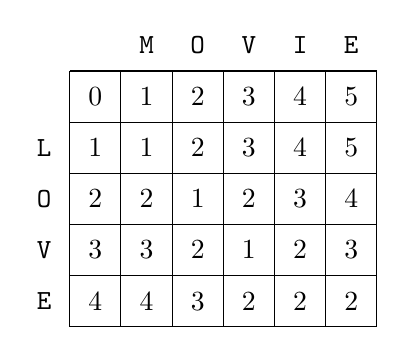
\begin{tikzpicture}[scale=.65]
  \begin{scope}
    %\fill [color=lightgray] (5, -3) rectangle (6, -4);
    \draw (1, -1) grid (7, -6);
    
    \node at (0.5,-2.5) {\texttt{L}};
    \node at (0.5,-3.5) {\texttt{O}};
    \node at (0.5,-4.5) {\texttt{V}};
    \node at (0.5,-5.5) {\texttt{E}};

    \node at (2.5,-0.5) {\texttt{M}};
    \node at (3.5,-0.5) {\texttt{O}};
    \node at (4.5,-0.5) {\texttt{V}};
    \node at (5.5,-0.5) {\texttt{I}};
    \node at (6.5,-0.5) {\texttt{E}};

    \node at (1.5,-1.5) {$0$};
    \node at (1.5,-2.5) {$1$};
    \node at (1.5,-3.5) {$2$};
    \node at (1.5,-4.5) {$3$};
    \node at (1.5,-5.5) {$4$};
    \node at (2.5,-1.5) {$1$};
    \node at (2.5,-2.5) {$1$};
    \node at (2.5,-3.5) {$2$};
    \node at (2.5,-4.5) {$3$};
    \node at (2.5,-5.5) {$4$};
    \node at (3.5,-1.5) {$2$};
    \node at (3.5,-2.5) {$2$};
    \node at (3.5,-3.5) {$1$};
    \node at (3.5,-4.5) {$2$};
    \node at (3.5,-5.5) {$3$};
    \node at (4.5,-1.5) {$3$};
    \node at (4.5,-2.5) {$3$};
    \node at (4.5,-3.5) {$2$};
    \node at (4.5,-4.5) {$1$};
    \node at (4.5,-5.5) {$2$};
    \node at (5.5,-1.5) {$4$};
    \node at (5.5,-2.5) {$4$};
    \node at (5.5,-3.5) {$3$};
    \node at (5.5,-4.5) {$2$};
    \node at (5.5,-5.5) {$2$};
    \node at (6.5,-1.5) {$5$};
    \node at (6.5,-2.5) {$5$};
    \node at (6.5,-3.5) {$4$};
    \node at (6.5,-4.5) {$3$};
    \node at (6.5,-5.5) {$2$};
  \end{scope}
\end{tikzpicture}
\end{center}

表格的右下角
告诉我们 \texttt{LOVE} 和 \texttt{MOVIE} 
之间的编辑距离为2。
表格还展示了如何构造
最短的编辑操作序列。
在这种情况下，路径如下：

\begin{center}
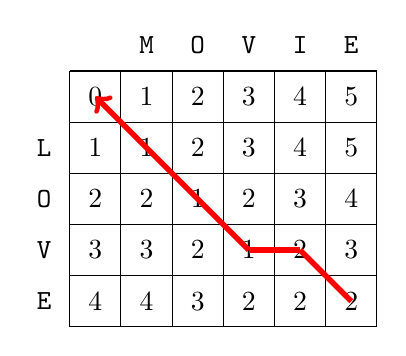
\begin{tikzpicture}[scale=.65]
  \begin{scope}
    \draw (1, -1) grid (7, -6);
    
    \node at (0.5,-2.5) {\texttt{L}};
    \node at (0.5,-3.5) {\texttt{O}};
    \node at (0.5,-4.5) {\texttt{V}};
    \node at (0.5,-5.5) {\texttt{E}};

    \node at (2.5,-0.5) {\texttt{M}};
    \node at (3.5,-0.5) {\texttt{O}};
    \node at (4.5,-0.5) {\texttt{V}};
    \node at (5.5,-0.5) {\texttt{I}};
    \node at (6.5,-0.5) {\texttt{E}};

    \node at (1.5,-1.5) {$0$};
    \node at (1.5,-2.5) {$1$};
    \node at (1.5,-3.5) {$2$};
    \node at (1.5,-4.5) {$3$};
    \node at (1.5,-5.5) {$4$};
    \node at (2.5,-1.5) {$1$};
    \node at (2.5,-2.5) {$1$};
    \node at (2.5,-3.5) {$2$};
    \node at (2.5,-4.5) {$3$};
    \node at (2.5,-5.5) {$4$};
    \node at (3.5,-1.5) {$2$};
    \node at (3.5,-2.5) {$2$};
    \node at (3.5,-3.5) {$1$};
    \node at (3.5,-4.5) {$2$};
    \node at (3.5,-5.5) {$3$};
    \node at (4.5,-1.5) {$3$};
    \node at (4.5,-2.5) {$3$};
    \node at (4.5,-3.5) {$2$};
    \node at (4.5,-4.5) {$1$};
    \node at (4.5,-5.5) {$2$};
    \node at (5.5,-1.5) {$4$};
    \node at (5.5,-2.5) {$4$};
    \node at (5.5,-3.5) {$3$};
    \node at (5.5,-4.5) {$2$};
    \node at (5.5,-5.5) {$2$};
    \node at (6.5,-1.5) {$5$};
    \node at (6.5,-2.5) {$5$};
    \node at (6.5,-3.5) {$4$};
    \node at (6.5,-4.5) {$3$};
    \node at (6.5,-5.5) {$2$};

    \path[draw=red,thick,-,line width=2pt] (6.5,-5.5) -- (5.5,-4.5);
    \path[draw=red,thick,-,line width=2pt] (5.5,-4.5) -- (4.5,-4.5);
    \path[draw=red,thick,->,line width=2pt] (4.5,-4.5) -- (1.5,-1.5);
  \end{scope}
\end{tikzpicture}
\end{center}

\texttt{LOVE} 和 \texttt{MOVIE} 的最后一个字符
相同，因此它们之间的编辑距离
等于 \texttt{LOV} 和 \texttt{MOVI} 之间的编辑距离。
我们可以用一次编辑操作从
\texttt{MOVI} 中删除字符 \texttt{I}。
因此，编辑距离比
\texttt{LOV} 和 \texttt{MOV} 之间的编辑距离大1，以此类推。

\section{计算铺方案}

有时动态规划解的状态
比数字的固定组合更加复杂。
作为一个例子，
考虑计算使用
$1 \times 2$ 和 $2 \times 1$ 大小的瓷砖
填充 $n \times m$ 网格的
不同方法数。
例如，$4 \times 7$ 网格的一个有效解是
\begin{center}
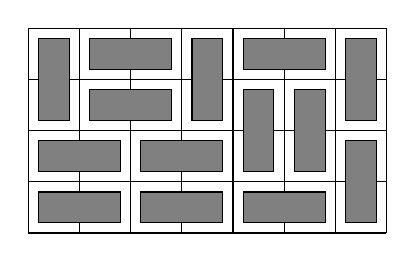
\begin{tikzpicture}[scale=.65]
    \draw (0,0) grid (7,4);
    \draw[fill=gray] (0+0.2,0+0.2) rectangle (2-0.2,1-0.2);
    \draw[fill=gray] (2+0.2,0+0.2) rectangle (4-0.2,1-0.2);
    \draw[fill=gray] (4+0.2,0+0.2) rectangle (6-0.2,1-0.2);
    \draw[fill=gray] (0+0.2,1+0.2) rectangle (2-0.2,2-0.2);
    \draw[fill=gray] (2+0.2,1+0.2) rectangle (4-0.2,2-0.2);
    \draw[fill=gray] (1+0.2,2+0.2) rectangle (3-0.2,3-0.2);
    \draw[fill=gray] (1+0.2,3+0.2) rectangle (3-0.2,4-0.2);
    \draw[fill=gray] (4+0.2,3+0.2) rectangle (6-0.2,4-0.2);

    \draw[fill=gray] (0+0.2,2+0.2) rectangle (1-0.2,4-0.2);
    \draw[fill=gray] (3+0.2,2+0.2) rectangle (4-0.2,4-0.2);
    \draw[fill=gray] (6+0.2,2+0.2) rectangle (7-0.2,4-0.2);
    \draw[fill=gray] (4+0.2,1+0.2) rectangle (5-0.2,3-0.2);
    \draw[fill=gray] (5+0.2,1+0.2) rectangle (6-0.2,3-0.2);
    \draw[fill=gray] (6+0.2,0+0.2) rectangle (7-0.2,2-0.2);

\end{tikzpicture}
\end{center}
总解数为781。

这个问题可以用动态规划解决，
方法是逐行遍历网格。
解中的每一行可以表示为
一个包含 $m$ 个字符的字符串，
字符取自集合
$\{\sqcap, \sqcup, \sqsubset, \sqsupset \}$。
例如，上述解由四行组成，
对应以下字符串：
\begin{itemize}
\item
$\sqcap \sqsubset \sqsupset \sqcap \sqsubset \sqsupset \sqcap$
\item
$\sqcup \sqsubset \sqsupset \sqcup \sqcap \sqcap \sqcup$
\item
$\sqsubset \sqsupset \sqsubset \sqsupset \sqcup \sqcup \sqcap$ 
\item
$\sqsubset \sqsupset \sqsubset \sqsupset \sqsubset \sqsupset \sqcup$
\end{itemize}

令 $\texttt{count}(k,x)$ 表示
为网格的第 $1 \ldots k$ 行
构造解的方法数，
其中字符串 $x$ 对应第 $k$ 行。
这里可以使用动态规划，
因为一行的状态仅受
前一行的状态约束。

一个解是有效的当且仅当第1行不包含
字符 $\sqcup$，
第 $n$ 行不包含字符 $\sqcap$，
且所有相邻行都是\emph{兼容的}。
例如，行
$\sqcup \sqsubset \sqsupset \sqcup \sqcap \sqcap \sqcup$ 和
$\sqsubset \sqsupset \sqsubset \sqsupset \sqcup \sqcup \sqcap$ 
是兼容的，而行
$\sqcap \sqsubset \sqsupset \sqcap \sqsubset \sqsupset \sqcap$ 和
$\sqsubset \sqsupset \sqsubset \sqsupset \sqsubset \sqsupset \sqcup$
是不兼容的。

由于一行由 $m$ 个字符组成，
每个字符有四种选择，
因此不同行的数量最多为 $4^m$。
因此，解决方案的时间复杂度为
$O(n 4^{2m})$，因为对于每一行，
我们需要遍历 $O(4^m)$ 个可能状态，
而对于每个状态，前一行的
可能状态有 $O(4^m)$ 个。
实际上，旋转网格使得
较短边的长度为 $m$ 是一个好主意，
因为因子 $4^{2m}$ 主导了时间复杂度。

通过使用更紧凑的行表示方法，
可以使解决方案更加高效。
事实上，只需要知道前一行的哪些列
包含竖直瓷砖的上半部分就足够了。
因此，我们可以仅使用字符
$\sqcap$ 和 $\Box$ 来表示一行，
其中 $\Box$ 是字符
$\sqcup$、$\sqsubset$ 和 $\sqsupset$ 的组合。
使用这种表示方法，
仅有 $2^m$ 种不同的行，
时间复杂度为 $O(n 2^{2m})$。

最后值得一提的是，还有一个令人惊讶的直接公式
用于计算铺方案数\footnote{令人惊讶的是，
这个公式是在1961年由两个研究团队 \cite{kas61,tem61}
独立发现的。}：
\[ \prod_{a=1}^{\lceil n/2 \rceil} \prod_{b=1}^{\lceil m/2 \rceil} 4 \cdot (\cos^2 \frac{\pi a}{n + 1} + \cos^2 \frac{\pi b}{m+1})\]
这个公式非常高效，因为它可以在 $O(nm)$ 时间内
计算出铺方案数，
但由于答案是实数的乘积，
使用该公式时的一个问题是
如何准确地存储中间结果。



\chapter{平摊分析}

\index{平摊分析}

算法的时间复杂度
通常很容易分析，
只需检查算法的结构：
算法包含哪些循环，
以及循环执行了多少次。
然而，有时简单的分析
并不能真实反映算法的效率。

\key{平摊分析}可以用来分析
包含时间复杂度变化的操作的算法。
其思想是估算算法执行期间
所有此类操作所使用的总时间，
而不是关注单个操作。

\section{双指针方法}

\index{双指针方法}

在\key{双指针方法}中，
使用两个指针来遍历数组的值。
两个指针都只能向一个方向移动，
这确保了算法的高效性。
接下来我们讨论两个可以使用
双指针方法解决的问题。

\subsubsection{子数组和}

作为第一个例子，
考虑这样一个问题：给定一个包含$n$个正整数的数组
和一个目标和$x$，
我们要找到一个和为$x$的子数组，
或者报告不存在这样的子数组。

例如，数组
\begin{center}
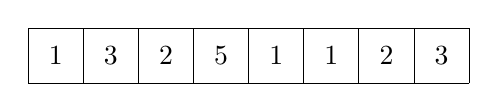
\begin{tikzpicture}[scale=0.7]
\draw (0,0) grid (8,1);

\node at (0.5,0.5) {$1$};
\node at (1.5,0.5) {$3$};
\node at (2.5,0.5) {$2$};
\node at (3.5,0.5) {$5$};
\node at (4.5,0.5) {$1$};
\node at (5.5,0.5) {$1$};
\node at (6.5,0.5) {$2$};
\node at (7.5,0.5) {$3$};
\end{tikzpicture}
\end{center}
包含一个和为8的子数组：
\begin{center}
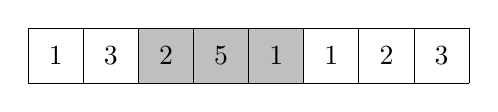
\begin{tikzpicture}[scale=0.7]
\fill[color=lightgray] (2,0) rectangle (5,1);
\draw (0,0) grid (8,1);

\node at (0.5,0.5) {$1$};
\node at (1.5,0.5) {$3$};
\node at (2.5,0.5) {$2$};
\node at (3.5,0.5) {$5$};
\node at (4.5,0.5) {$1$};
\node at (5.5,0.5) {$1$};
\node at (6.5,0.5) {$2$};
\node at (7.5,0.5) {$3$};
\end{tikzpicture}
\end{center}

这个问题可以使用双指针方法
在$O(n)$时间内解决。
其思想是维护指向子数组
第一个和最后一个值的指针。
在每一轮中，左指针向右移动一步，
右指针则向右移动，
只要结果子数组的和不超过$x$。
如果和恰好等于$x$，
就找到了一个解。

作为例子，考虑以下数组
和目标和$x=8$：
\begin{center}
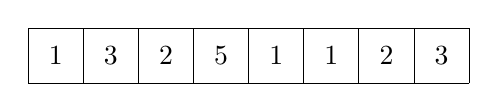
\begin{tikzpicture}[scale=0.7]
\draw (0,0) grid (8,1);

\node at (0.5,0.5) {$1$};
\node at (1.5,0.5) {$3$};
\node at (2.5,0.5) {$2$};
\node at (3.5,0.5) {$5$};
\node at (4.5,0.5) {$1$};
\node at (5.5,0.5) {$1$};
\node at (6.5,0.5) {$2$};
\node at (7.5,0.5) {$3$};
\end{tikzpicture}
\end{center}

初始子数组包含值
1、3和2，其和为6：

\begin{center}
\begin{tikzpicture}[scale=0.7]
\fill[color=lightgray] (0,0) rectangle (3,1);
\draw (0,0) grid (8,1);

\node at (0.5,0.5) {$1$};
\node at (1.5,0.5) {$3$};
\node at (2.5,0.5) {$2$};
\node at (3.5,0.5) {$5$};
\node at (4.5,0.5) {$1$};
\node at (5.5,0.5) {$1$};
\node at (6.5,0.5) {$2$};
\node at (7.5,0.5) {$3$};

\draw[thick,->] (0.5,-0.7) -- (0.5,-0.1);
\draw[thick,->] (2.5,-0.7) -- (2.5,-0.1);
\end{tikzpicture}
\end{center}

然后，左指针向右移动一步。
右指针不动，因为否则
子数组的和将超过$x$。

\begin{center}
\begin{tikzpicture}[scale=0.7]
\fill[color=lightgray] (1,0) rectangle (3,1);
\draw (0,0) grid (8,1);

\node at (0.5,0.5) {$1$};
\node at (1.5,0.5) {$3$};
\node at (2.5,0.5) {$2$};
\node at (3.5,0.5) {$5$};
\node at (4.5,0.5) {$1$};
\node at (5.5,0.5) {$1$};
\node at (6.5,0.5) {$2$};
\node at (7.5,0.5) {$3$};

\draw[thick,->] (1.5,-0.7) -- (1.5,-0.1);
\draw[thick,->] (2.5,-0.7) -- (2.5,-0.1);
\end{tikzpicture}
\end{center}

再一次，左指针向右移动一步，
这次右指针向右移动了三步。
子数组的和为$2+5+1=8$，因此找到了
一个和为$x$的子数组。

\begin{center}
\begin{tikzpicture}[scale=0.7]
\fill[color=lightgray] (2,0) rectangle (5,1);
\draw (0,0) grid (8,1);

\node at (0.5,0.5) {$1$};
\node at (1.5,0.5) {$3$};
\node at (2.5,0.5) {$2$};
\node at (3.5,0.5) {$5$};
\node at (4.5,0.5) {$1$};
\node at (5.5,0.5) {$1$};
\node at (6.5,0.5) {$2$};
\node at (7.5,0.5) {$3$};

\draw[thick,->] (2.5,-0.7) -- (2.5,-0.1);
\draw[thick,->] (4.5,-0.7) -- (4.5,-0.1);
\end{tikzpicture}
\end{center}

算法的运行时间取决于
右指针移动的步数。
虽然在\emph{单次}操作中
指针移动的步数没有有用的上界，
但我们知道在算法执行期间指针总共移动了
\emph{总共}$O(n)$步，
因为它只向右移动。

由于左指针和右指针
在算法执行期间都移动$O(n)$步，
因此算法的运行时间为$O(n)$。

\subsubsection{2SUM问题}

\index{2SUM问题}

另一个可以使用
双指针方法解决的问题是
以下问题，也称为\key{2SUM问题}：
给定一个包含$n$个数的数组
和一个目标和$x$，找出
两个数组值使其和为$x$，
或者报告不存在这样的值。

为了解决这个问题，我们首先
将数组值按递增顺序排序。
然后，我们使用两个指针遍历数组。
左指针从第一个值开始，
每轮向右移动一步。
右指针从最后一个值开始，
始终向左移动，直到左右
值之和不超过$x$。
如果和恰好等于$x$，
就找到了一个解。

例如，考虑以下数组
和目标和$x=12$：
\begin{center}
\begin{tikzpicture}[scale=0.7]
\draw (0,0) grid (8,1);

\node at (0.5,0.5) {$1$};
\node at (1.5,0.5) {$4$};
\node at (2.5,0.5) {$5$};
\node at (3.5,0.5) {$6$};
\node at (4.5,0.5) {$7$};
\node at (5.5,0.5) {$9$};
\node at (6.5,0.5) {$9$};
\node at (7.5,0.5) {$10$};
\end{tikzpicture}
\end{center}

指针的初始位置
如下所示。
值之和为$1+10=11$，
小于$x$。

\begin{center}
\begin{tikzpicture}[scale=0.7]
\fill[color=lightgray] (0,0) rectangle (1,1);
\fill[color=lightgray] (7,0) rectangle (8,1);
\draw (0,0) grid (8,1);

\node at (0.5,0.5) {$1$};
\node at (1.5,0.5) {$4$};
\node at (2.5,0.5) {$5$};
\node at (3.5,0.5) {$6$};
\node at (4.5,0.5) {$7$};
\node at (5.5,0.5) {$9$};
\node at (6.5,0.5) {$9$};
\node at (7.5,0.5) {$10$};

\draw[thick,->] (0.5,-0.7) -- (0.5,-0.1);
\draw[thick,->] (7.5,-0.7) -- (7.5,-0.1);
\end{tikzpicture}
\end{center}

然后左指针向右移动一步。
右指针向左移动三步，
和变为$4+7=11$。

\begin{center}
\begin{tikzpicture}[scale=0.7]
\fill[color=lightgray] (1,0) rectangle (2,1);
\fill[color=lightgray] (4,0) rectangle (5,1);
\draw (0,0) grid (8,1);

\node at (0.5,0.5) {$1$};
\node at (1.5,0.5) {$4$};
\node at (2.5,0.5) {$5$};
\node at (3.5,0.5) {$6$};
\node at (4.5,0.5) {$7$};
\node at (5.5,0.5) {$9$};
\node at (6.5,0.5) {$9$};
\node at (7.5,0.5) {$10$};

\draw[thick,->] (1.5,-0.7) -- (1.5,-0.1);
\draw[thick,->] (4.5,-0.7) -- (4.5,-0.1);
\end{tikzpicture}
\end{center}

之后，左指针再次向右移动一步。
右指针不动，找到了一个解
$5+7=12$。

\begin{center}
\begin{tikzpicture}[scale=0.7]
\fill[color=lightgray] (2,0) rectangle (3,1);
\fill[color=lightgray] (4,0) rectangle (5,1);
\draw (0,0) grid (8,1);

\node at (0.5,0.5) {$1$};
\node at (1.5,0.5) {$4$};
\node at (2.5,0.5) {$5$};
\node at (3.5,0.5) {$6$};
\node at (4.5,0.5) {$7$};
\node at (5.5,0.5) {$9$};
\node at (6.5,0.5) {$9$};
\node at (7.5,0.5) {$10$};

\draw[thick,->] (2.5,-0.7) -- (2.5,-0.1);
\draw[thick,->] (4.5,-0.7) -- (4.5,-0.1);
\end{tikzpicture}
\end{center}

算法的运行时间为
$O(n \log n)$，因为它首先
在$O(n \log n)$时间内对数组排序，
然后两个指针各移动$O(n)$步。

注意，也可以使用二分搜索
以另一种方式在$O(n \log n)$时间内
解决这个问题。
在这种解法中，我们遍历数组，
对于每个数组值，尝试找到另一个
值使其与该值之和为$x$。
这可以通过执行$n$次二分搜索来完成，
每次二分搜索耗时$O(\log n)$。

\index{3SUM问题}
一个更难的问题是
\key{3SUM问题}，要求找到
\emph{三个}数组值
使其和为$x$。
利用上述算法的思想，
这个问题可以在$O(n^2)$时间内解决\footnote{长期以来，
人们认为比$O(n^2)$时间
更高效地解决
3SUM问题是不可能的。
然而，2014年的研究 \cite{gro14}
表明事实并非如此。}。
你能想到怎么做吗？

\section{最近较小元素}

\index{最近较小元素}

平摊分析常用于估算
在数据结构上执行的操作次数。
这些操作可能分布不均匀，
即大部分操作发生在算法的某个
特定阶段，但操作的总数
是有限的。

作为例子，考虑如下问题：
为每个数组元素找到
\key{最近较小元素}，即
在数组中位于该元素之前的第一个
更小的元素。
可能不存在这样的元素，
此时算法应报告这一情况。
接下来我们将看到如何使用栈结构
高效地解决这个问题。

我们从左到右遍历数组，
并维护一个由数组元素组成的栈。
在每个数组位置，我们从栈中移除元素，
直到栈顶元素小于当前元素，
或者栈为空。
然后，我们报告栈顶元素为
当前元素的最近较小元素，
如果栈为空，则不存在这样的元素。
最后，我们将当前元素添加到栈中。

作为例子，考虑以下数组：
\begin{center}
\begin{tikzpicture}[scale=0.7]
\draw (0,0) grid (8,1);

\node at (0.5,0.5) {$1$};
\node at (1.5,0.5) {$3$};
\node at (2.5,0.5) {$4$};
\node at (3.5,0.5) {$2$};
\node at (4.5,0.5) {$5$};
\node at (5.5,0.5) {$3$};
\node at (6.5,0.5) {$4$};
\node at (7.5,0.5) {$2$};
\end{tikzpicture}
\end{center}

首先，元素1、3和4被添加到栈中，
因为每个元素都比前一个元素大。
因此，4的最近较小元素是3，
3的最近较小元素是1。
\begin{center}
\begin{tikzpicture}[scale=0.7]
\fill[color=lightgray] (2,0) rectangle (3,1);
\draw (0,0) grid (8,1);

\node at (0.5,0.5) {$1$};
\node at (1.5,0.5) {$3$};
\node at (2.5,0.5) {$4$};
\node at (3.5,0.5) {$2$};
\node at (4.5,0.5) {$5$};
\node at (5.5,0.5) {$3$};
\node at (6.5,0.5) {$4$};
\node at (7.5,0.5) {$2$};

\draw (0.2,0.2-1.2) rectangle (0.8,0.8-1.2);
\draw (1.2,0.2-1.2) rectangle (1.8,0.8-1.2);
\draw (2.2,0.2-1.2) rectangle (2.8,0.8-1.2);

\node at (0.5,0.5-1.2) {$1$};
\node at (1.5,0.5-1.2) {$3$};
\node at (2.5,0.5-1.2) {$4$};

\draw[->,thick] (0.8,0.5-1.2) -- (1.2,0.5-1.2);
\draw[->,thick] (1.8,0.5-1.2) -- (2.2,0.5-1.2);
\end{tikzpicture}
\end{center}

下一个元素2比栈顶的
两个元素小。
因此，元素3和4从栈中移除，
然后元素2被添加到栈中。
它的最近较小元素是1：
\begin{center}
\begin{tikzpicture}[scale=0.7]
\fill[color=lightgray] (3,0) rectangle (4,1);
\draw (0,0) grid (8,1);

\node at (0.5,0.5) {$1$};
\node at (1.5,0.5) {$3$};
\node at (2.5,0.5) {$4$};
\node at (3.5,0.5) {$2$};
\node at (4.5,0.5) {$5$};
\node at (5.5,0.5) {$3$};
\node at (6.5,0.5) {$4$};
\node at (7.5,0.5) {$2$};

\draw (0.2,0.2-1.2) rectangle (0.8,0.8-1.2);
\draw (3.2,0.2-1.2) rectangle (3.8,0.8-1.2);

\node at (0.5,0.5-1.2) {$1$};
\node at (3.5,0.5-1.2) {$2$};

\draw[->,thick] (0.8,0.5-1.2) -- (3.2,0.5-1.2);
\end{tikzpicture}
\end{center}

然后，元素5比元素2大，
所以它被添加到栈中，
其最近较小元素是2：
\begin{center}
\begin{tikzpicture}[scale=0.7]
\fill[color=lightgray] (4,0) rectangle (5,1);
\draw (0,0) grid (8,1);

\node at (0.5,0.5) {$1$};
\node at (1.5,0.5) {$3$};
\node at (2.5,0.5) {$4$};
\node at (3.5,0.5) {$2$};
\node at (4.5,0.5) {$5$};
\node at (5.5,0.5) {$3$};
\node at (6.5,0.5) {$4$};
\node at (7.5,0.5) {$2$};

\draw (0.2,0.2-1.2) rectangle (0.8,0.8-1.2);
\draw (3.2,0.2-1.2) rectangle (3.8,0.8-1.2);
\draw (4.2,0.2-1.2) rectangle (4.8,0.8-1.2);

\node at (0.5,0.5-1.2) {$1$};
\node at (3.5,0.5-1.2) {$2$};
\node at (4.5,0.5-1.2) {$5$};

\draw[->,thick] (0.8,0.5-1.2) -- (3.2,0.5-1.2);
\draw[->,thick] (3.8,0.5-1.2) -- (4.2,0.5-1.2);
\end{tikzpicture}
\end{center}

之后，元素5从栈中移除，
元素3和4被添加到栈中：
\begin{center}
\begin{tikzpicture}[scale=0.7]
\fill[color=lightgray] (6,0) rectangle (7,1);
\draw (0,0) grid (8,1);

\node at (0.5,0.5) {$1$};
\node at (1.5,0.5) {$3$};
\node at (2.5,0.5) {$4$};
\node at (3.5,0.5) {$2$};
\node at (4.5,0.5) {$5$};
\node at (5.5,0.5) {$3$};
\node at (6.5,0.5) {$4$};
\node at (7.5,0.5) {$2$};

\draw (0.2,0.2-1.2) rectangle (0.8,0.8-1.2);
\draw (3.2,0.2-1.2) rectangle (3.8,0.8-1.2);
\draw (5.2,0.2-1.2) rectangle (5.8,0.8-1.2);
\draw (6.2,0.2-1.2) rectangle (6.8,0.8-1.2);

\node at (0.5,0.5-1.2) {$1$};
\node at (3.5,0.5-1.2) {$2$};
\node at (5.5,0.5-1.2) {$3$};
\node at (6.5,0.5-1.2) {$4$};

\draw[->,thick] (0.8,0.5-1.2) -- (3.2,0.5-1.2);
\draw[->,thick] (3.8,0.5-1.2) -- (5.2,0.5-1.2);
\draw[->,thick] (5.8,0.5-1.2) -- (6.2,0.5-1.2);
\end{tikzpicture}
\end{center}

最后，除1之外的所有元素
都从栈中移除，最后一个元素2
被添加到栈中：

\begin{center}
\begin{tikzpicture}[scale=0.7]
\fill[color=lightgray] (7,0) rectangle (8,1);
\draw (0,0) grid (8,1);

\node at (0.5,0.5) {$1$};
\node at (1.5,0.5) {$3$};
\node at (2.5,0.5) {$4$};
\node at (3.5,0.5) {$2$};
\node at (4.5,0.5) {$5$};
\node at (5.5,0.5) {$3$};
\node at (6.5,0.5) {$4$};
\node at (7.5,0.5) {$2$};

\draw (0.2,0.2-1.2) rectangle (0.8,0.8-1.2);
\draw (7.2,0.2-1.2) rectangle (7.8,0.8-1.2);

\node at (0.5,0.5-1.2) {$1$};
\node at (7.5,0.5-1.2) {$2$};

\draw[->,thick] (0.8,0.5-1.2) -- (7.2,0.5-1.2);
\end{tikzpicture}
\end{center}

算法的效率取决于
栈操作的总次数。
如果当前元素大于
栈顶元素，它直接被
添加到栈中，这是高效的。
然而，有时栈中可能包含多个
更大的元素，移除它们需要时间。
尽管如此，每个元素\emph{恰好一次}被添加到栈中，
并且\emph{至多一次}从栈中移除。
因此，每个元素引起$O(1)$次栈操作，
算法的运行时间为$O(n)$。

\section{滑动窗口最小值}

\index{滑动窗口}
\index{滑动窗口最小值}

\key{滑动窗口}是一个固定大小的子数组，
它从左到右穿过数组。
在每个窗口位置，
我们想计算关于
窗口内元素的一些信息。
在本节中，我们关注
维护\key{滑动窗口最小值}的问题，
也就是说
我们应该报告每个窗口内的最小值。

滑动窗口最小值可以使用
与我们计算最近较小元素时类似的思想来计算。
我们维护一个队列，
其中每个元素都大于
前一个元素，
而第一个元素
始终对应窗口内的最小元素。
在每次窗口移动后，
我们从队列末尾移除元素，
直到最后一个队列元素
小于新的窗口元素，
或者队列变空。
如果队列中的第一个元素
不再位于窗口内，我们也将其移除。
最后，我们将新的窗口元素
添加到队列末尾。

作为例子，考虑以下数组：

\begin{center}
\begin{tikzpicture}[scale=0.7]
\draw (0,0) grid (8,1);

\node at (0.5,0.5) {$2$};
\node at (1.5,0.5) {$1$};
\node at (2.5,0.5) {$4$};
\node at (3.5,0.5) {$5$};
\node at (4.5,0.5) {$3$};
\node at (5.5,0.5) {$4$};
\node at (6.5,0.5) {$1$};
\node at (7.5,0.5) {$2$};
\end{tikzpicture}
\end{center}

假设滑动窗口的大小为4。
在第一个窗口位置，最小值为1：
\begin{center}
\begin{tikzpicture}[scale=0.7]
\fill[color=lightgray] (0,0) rectangle (4,1);
\draw (0,0) grid (8,1);

\node at (0.5,0.5) {$2$};
\node at (1.5,0.5) {$1$};
\node at (2.5,0.5) {$4$};
\node at (3.5,0.5) {$5$};
\node at (4.5,0.5) {$3$};
\node at (5.5,0.5) {$4$};
\node at (6.5,0.5) {$1$};
\node at (7.5,0.5) {$2$};

\draw (1.2,0.2-1.2) rectangle (1.8,0.8-1.2);
\draw (2.2,0.2-1.2) rectangle (2.8,0.8-1.2);
\draw (3.2,0.2-1.2) rectangle (3.8,0.8-1.2);

\node at (1.5,0.5-1.2) {$1$};
\node at (2.5,0.5-1.2) {$4$};
\node at (3.5,0.5-1.2) {$5$};

\draw[->,thick] (1.8,0.5-1.2) -- (2.2,0.5-1.2);
\draw[->,thick] (2.8,0.5-1.2) -- (3.2,0.5-1.2);
\end{tikzpicture}
\end{center}

然后窗口向右移动一步。
新元素3比队列中的
元素4和5小，因此元素4和5
从队列中移除，
元素3被添加到队列中。
最小值仍为1。
\begin{center}
\begin{tikzpicture}[scale=0.7]
\fill[color=lightgray] (1,0) rectangle (5,1);
\draw (0,0) grid (8,1);

\node at (0.5,0.5) {$2$};
\node at (1.5,0.5) {$1$};
\node at (2.5,0.5) {$4$};
\node at (3.5,0.5) {$5$};
\node at (4.5,0.5) {$3$};
\node at (5.5,0.5) {$4$};
\node at (6.5,0.5) {$1$};
\node at (7.5,0.5) {$2$};

\draw (1.2,0.2-1.2) rectangle (1.8,0.8-1.2);
\draw (4.2,0.2-1.2) rectangle (4.8,0.8-1.2);

\node at (1.5,0.5-1.2) {$1$};
\node at (4.5,0.5-1.2) {$3$};

\draw[->,thick] (1.8,0.5-1.2) -- (4.2,0.5-1.2);
\end{tikzpicture}
\end{center}

之后，窗口再次移动，
最小元素1
不再属于窗口。
因此，它从队列中移除，
最小值现在是3。同时新元素4
被添加到队列中。
\begin{center}
\begin{tikzpicture}[scale=0.7]
\fill[color=lightgray] (2,0) rectangle (6,1);
\draw (0,0) grid (8,1);

\node at (0.5,0.5) {$2$};
\node at (1.5,0.5) {$1$};
\node at (2.5,0.5) {$4$};
\node at (3.5,0.5) {$5$};
\node at (4.5,0.5) {$3$};
\node at (5.5,0.5) {$4$};
\node at (6.5,0.5) {$1$};
\node at (7.5,0.5) {$2$};

\draw (4.2,0.2-1.2) rectangle (4.8,0.8-1.2);
\draw (5.2,0.2-1.2) rectangle (5.8,0.8-1.2);

\node at (4.5,0.5-1.2) {$3$};
\node at (5.5,0.5-1.2) {$4$};

\draw[->,thick] (4.8,0.5-1.2) -- (5.2,0.5-1.2);
\end{tikzpicture}
\end{center}

下一个新元素1比队列中的
所有元素都小。
因此，所有元素都从队列中移除，
队列中将只包含元素1：
\begin{center}
\begin{tikzpicture}[scale=0.7]
\fill[color=lightgray] (3,0) rectangle (7,1);
\draw (0,0) grid (8,1);

\node at (0.5,0.5) {$2$};
\node at (1.5,0.5) {$1$};
\node at (2.5,0.5) {$4$};
\node at (3.5,0.5) {$5$};
\node at (4.5,0.5) {$3$};
\node at (5.5,0.5) {$4$};
\node at (6.5,0.5) {$1$};
\node at (7.5,0.5) {$2$};

\draw (6.2,0.2-1.2) rectangle (6.8,0.8-1.2);

\node at (6.5,0.5-1.2) {$1$};
\end{tikzpicture}
\end{center}

最后窗口到达其最后一个位置。
元素2被添加到队列中，
但窗口内的最小值
仍为1。
\begin{center}
\begin{tikzpicture}[scale=0.7]
\fill[color=lightgray] (4,0) rectangle (8,1);
\draw (0,0) grid (8,1);

\node at (0.5,0.5) {$2$};
\node at (1.5,0.5) {$1$};
\node at (2.5,0.5) {$4$};
\node at (3.5,0.5) {$5$};
\node at (4.5,0.5) {$3$};
\node at (5.5,0.5) {$4$};
\node at (6.5,0.5) {$1$};
\node at (7.5,0.5) {$2$};

\draw (6.2,0.2-1.2) rectangle (6.8,0.8-1.2);
\draw (7.2,0.2-1.2) rectangle (7.8,0.8-1.2);

\node at (6.5,0.5-1.2) {$1$};
\node at (7.5,0.5-1.2) {$2$};

\draw[->,thick] (6.8,0.5-1.2) -- (7.2,0.5-1.2);
\end{tikzpicture}
\end{center}

由于每个数组元素
恰好一次被添加到队列中，
并且至多一次从队列中移除，
因此算法的运行时间为$O(n)$。




\chapter{区间查询}

\index{区间查询}
\index{求和查询}
\index{最小值查询}
\index{最大值查询}

在本章中，我们讨论能够高效处理区间查询的
数据结构。
在\key{区间查询}中，
我们的任务是
基于数组的一个子数组来计算一个值。
典型的区间查询包括：
\begin{itemize}
\item $\texttt{sum}_q(a,b)$：计算区间 $[a,b]$ 中值的总和
\item $\texttt{min}_q(a,b)$：找出区间 $[a,b]$ 中的最小值
\item $\texttt{max}_q(a,b)$：找出区间 $[a,b]$ 中的最大值
\end{itemize}

例如，考虑以下数组中的区间 $[3,6]$：
\begin{center}
\begin{tikzpicture}[scale=0.7]
\fill[color=lightgray] (3,0) rectangle (7,1);
\draw (0,0) grid (8,1);

\node at (0.5,0.5) {$1$};
\node at (1.5,0.5) {$3$};
\node at (2.5,0.5) {$8$};
\node at (3.5,0.5) {$4$};
\node at (4.5,0.5) {$6$};
\node at (5.5,0.5) {$1$};
\node at (6.5,0.5) {$3$};
\node at (7.5,0.5) {$4$};

\footnotesize
\node at (0.5,1.4) {$0$};
\node at (1.5,1.4) {$1$};
\node at (2.5,1.4) {$2$};
\node at (3.5,1.4) {$3$};
\node at (4.5,1.4) {$4$};
\node at (5.5,1.4) {$5$};
\node at (6.5,1.4) {$6$};
\node at (7.5,1.4) {$7$};
\end{tikzpicture}
\end{center}
在这种情况下，$\texttt{sum}_q(3,6)=14$，
$\texttt{min}_q(3,6)=1$，$\texttt{max}_q(3,6)=6$。

处理区间查询的一种简单方法是使用
一个循环遍历区间内的所有数组值。
例如，以下函数可用于
处理数组上的求和查询：

\begin{lstlisting}
int sum(int a, int b) {
    int s = 0;
    for (int i = a; i <= b; i++) {
        s += array[i];
    }
    return s;
}
\end{lstlisting}

该函数的时间复杂度为 $O(n)$，
其中 $n$ 是数组的大小。
因此，使用该函数我们可以在 $O(nq)$
时间内处理 $q$ 个查询。
然而，如果 $n$ 和 $q$ 都很大，这种方法就很慢。
幸运的是，事实证明有多种方法
可以更加高效地处理区间查询。

\section{静态数组查询}

我们首先关注数组是\emph{静态}的情况，
即数组值在查询之间不会被更新。
在这种情况下，只需构造一个静态数据结构，
它就能告诉我们任意可能的查询的答案。

\subsubsection{求和查询}

\index{前缀和数组}

我们可以通过构造\key{前缀和数组}
来轻松处理静态数组上的求和查询。
前缀和数组中的每个值等于
原数组中从开头到该位置的所有值之和，
即位置 $k$ 处的值为 $\texttt{sum}_q(0,k)$。
前缀和数组可以在 $O(n)$ 时间内构造完成。

例如，考虑以下数组：
\begin{center}
\begin{tikzpicture}[scale=0.7]
%\fill[color=lightgray] (3,0) rectangle (7,1);
\draw (0,0) grid (8,1);

\node at (0.5,0.5) {$1$};
\node at (1.5,0.5) {$3$};
\node at (2.5,0.5) {$4$};
\node at (3.5,0.5) {$8$};
\node at (4.5,0.5) {$6$};
\node at (5.5,0.5) {$1$};
\node at (6.5,0.5) {$4$};
\node at (7.5,0.5) {$2$};

\footnotesize
\node at (0.5,1.4) {$0$};
\node at (1.5,1.4) {$1$};
\node at (2.5,1.4) {$2$};
\node at (3.5,1.4) {$3$};
\node at (4.5,1.4) {$4$};
\node at (5.5,1.4) {$5$};
\node at (6.5,1.4) {$6$};
\node at (7.5,1.4) {$7$};
\end{tikzpicture}
\end{center}
对应的前缀和数组如下：
\begin{center}
\begin{tikzpicture}[scale=0.7]
%\fill[color=lightgray] (3,0) rectangle (7,1);
\draw (0,0) grid (8,1);

\node at (0.5,0.5) {$1$};
\node at (1.5,0.5) {$4$};
\node at (2.5,0.5) {$8$};
\node at (3.5,0.5) {$16$};
\node at (4.5,0.5) {$22$};
\node at (5.5,0.5) {$23$};
\node at (6.5,0.5) {$27$};
\node at (7.5,0.5) {$29$};


\footnotesize
\node at (0.5,1.4) {$0$};
\node at (1.5,1.4) {$1$};
\node at (2.5,1.4) {$2$};
\node at (3.5,1.4) {$3$};
\node at (4.5,1.4) {$4$};
\node at (5.5,1.4) {$5$};
\node at (6.5,1.4) {$6$};
\node at (7.5,1.4) {$7$};
\end{tikzpicture}
\end{center}
由于前缀和数组包含了
$\texttt{sum}_q(0,k)$ 的所有值，
我们可以在 $O(1)$ 时间内
按以下方式计算任意
$\texttt{sum}_q(a,b)$ 的值：
\[ \texttt{sum}_q(a,b) = \texttt{sum}_q(0,b) - \texttt{sum}_q(0,a-1)\]
通过定义 $\texttt{sum}_q(0,-1)=0$，
上述公式在 $a=0$ 时同样成立。

例如，考虑区间 $[3,6]$：
\begin{center}
\begin{tikzpicture}[scale=0.7]
\fill[color=lightgray] (3,0) rectangle (7,1);
\draw (0,0) grid (8,1);

\node at (0.5,0.5) {$1$};
\node at (1.5,0.5) {$3$};
\node at (2.5,0.5) {$4$};
\node at (3.5,0.5) {$8$};
\node at (4.5,0.5) {$6$};
\node at (5.5,0.5) {$1$};
\node at (6.5,0.5) {$4$};
\node at (7.5,0.5) {$2$};

\footnotesize
\node at (0.5,1.4) {$0$};
\node at (1.5,1.4) {$1$};
\node at (2.5,1.4) {$2$};
\node at (3.5,1.4) {$3$};
\node at (4.5,1.4) {$4$};
\node at (5.5,1.4) {$5$};
\node at (6.5,1.4) {$6$};
\node at (7.5,1.4) {$7$};
\end{tikzpicture}
\end{center}
在这种情况下 $\texttt{sum}_q(3,6)=8+6+1+4=19$。
这个和可以从
前缀和数组中的两个值计算得出：
\begin{center}
\begin{tikzpicture}[scale=0.7]
\fill[color=lightgray] (2,0) rectangle (3,1);
\fill[color=lightgray] (6,0) rectangle (7,1);
\draw (0,0) grid (8,1);

\node at (0.5,0.5) {$1$};
\node at (1.5,0.5) {$4$};
\node at (2.5,0.5) {$8$};
\node at (3.5,0.5) {$16$};
\node at (4.5,0.5) {$22$};
\node at (5.5,0.5) {$23$};
\node at (6.5,0.5) {$27$};
\node at (7.5,0.5) {$29$};

\footnotesize
\node at (0.5,1.4) {$0$};
\node at (1.5,1.4) {$1$};
\node at (2.5,1.4) {$2$};
\node at (3.5,1.4) {$3$};
\node at (4.5,1.4) {$4$};
\node at (5.5,1.4) {$5$};
\node at (6.5,1.4) {$6$};
\node at (7.5,1.4) {$7$};
\end{tikzpicture}
\end{center}
因此，$\texttt{sum}_q(3,6)=\texttt{sum}_q(0,6)-\texttt{sum}_q(0,2)=27-8=19$。

这个思想也可以推广
到更高维度。
例如，我们可以构造一个二维
前缀和数组，用于在 $O(1)$ 时间内
计算任意矩形子数组的和。
该数组中的每个和对应于
一个从数组左上角
开始的子数组。

\begin{samepage}
下图说明了这个思想：
\begin{center}
\begin{tikzpicture}[scale=0.54]
\draw[fill=lightgray] (3,2) rectangle (7,5);
\draw (0,0) grid (10,7);
\node[anchor=center] at (6.5, 2.5) {$A$};
\node[anchor=center] at (2.5, 2.5) {$B$};
\node[anchor=center] at (6.5, 5.5) {$C$};
\node[anchor=center] at (2.5, 5.5) {$D$};
\end{tikzpicture}
\end{center}
\end{samepage}

灰色子数组的和可以用
以下公式计算
\[S(A) - S(B) - S(C) + S(D),\]
其中 $S(X)$ 表示从数组左上角
到 $X$ 的位置的
矩形子数组中值的和。

\subsubsection{最小值查询}

\index{稀疏表}

最小值查询比求和查询更难处理。
不过，有一种相当简单的
$O(n \log n)$ 时间预处理方法，
预处理之后我们可以在 $O(1)$ 时间内
回答任意最小值查询\footnote{该技术
在 \cite{ben00} 中被提出，有时
被称为\key{稀疏表}方法。
还有更复杂的技术 \cite{fis06}，其预处理时间仅为 $O(n)$，
但这种算法在竞赛编程中并不需要。}。
注意，由于最小值查询和最大值查询的处理方式类似，
我们可以只关注最小值查询。

核心思想是预先计算
$b-a+1$（区间长度）为 2 的幂的
所有 $\textrm{min}_q(a,b)$ 的值。
例如，对于以下数组

\begin{center}
\begin{tikzpicture}[scale=0.7]
\draw (0,0) grid (8,1);

\node at (0.5,0.5) {$1$};
\node at (1.5,0.5) {$3$};
\node at (2.5,0.5) {$4$};
\node at (3.5,0.5) {$8$};
\node at (4.5,0.5) {$6$};
\node at (5.5,0.5) {$1$};
\node at (6.5,0.5) {$4$};
\node at (7.5,0.5) {$2$};

\footnotesize
\node at (0.5,1.4) {$0$};
\node at (1.5,1.4) {$1$};
\node at (2.5,1.4) {$2$};
\node at (3.5,1.4) {$3$};
\node at (4.5,1.4) {$4$};
\node at (5.5,1.4) {$5$};
\node at (6.5,1.4) {$6$};
\node at (7.5,1.4) {$7$};
\end{tikzpicture}
\end{center}
可以计算出以下值：

\begin{center}
\begin{tabular}{ccc}

\begin{tabular}{lll}
$a$ & $b$ & $\texttt{min}_q(a,b)$ \\
\hline
0 & 0 & 1 \\
1 & 1 & 3 \\
2 & 2 & 4 \\
3 & 3 & 8 \\
4 & 4 & 6 \\
5 & 5 & 1 \\
6 & 6 & 4 \\
7 & 7 & 2 \\
\end{tabular}

&

\begin{tabular}{lll}
$a$ & $b$ & $\texttt{min}_q(a,b)$ \\
\hline
0 & 1 & 1 \\
1 & 2 & 3 \\
2 & 3 & 4 \\
3 & 4 & 6 \\
4 & 5 & 1 \\
5 & 6 & 1 \\
6 & 7 & 2 \\
\\
\end{tabular}

&

\begin{tabular}{lll}
$a$ & $b$ & $\texttt{min}_q(a,b)$ \\
\hline
0 & 3 & 1 \\
1 & 4 & 3 \\
2 & 5 & 1 \\
3 & 6 & 1 \\
4 & 7 & 1 \\
0 & 7 & 1 \\
\\
\\
\end{tabular}

\end{tabular}
\end{center}

预计算值的数量为 $O(n \log n)$，
因为作为 2 的幂的区间长度
有 $O(\log n)$ 种。
这些值可以使用以下递归公式
高效地计算
\[\texttt{min}_q(a,b) = \min(\texttt{min}_q(a,a+w-1),\texttt{min}_q(a+w,b)),\]
其中 $b-a+1$ 是 2 的幂，$w=(b-a+1)/2$。
计算所有这些值需要 $O(n \log n)$ 时间。

之后，任何 $\texttt{min}_q(a,b)$ 的值都可以
在 $O(1)$ 时间内计算出来，即两个预计算值的最小值。
设 $k$ 为不超过 $b-a+1$ 的最大 2 的幂。
我们可以使用以下公式计算 $\texttt{min}_q(a,b)$ 的值
\[\texttt{min}_q(a,b) = \min(\texttt{min}_q(a,a+k-1),\texttt{min}_q(b-k+1,b)).\]
在上述公式中，区间 $[a,b]$ 被表示为
区间 $[a,a+k-1]$ 和 $[b-k+1,b]$ 的并集，两者的长度均为 $k$。

作为一个例子，考虑区间 $[1,6]$：
\begin{center}
\begin{tikzpicture}[scale=0.7]
\fill[color=lightgray] (1,0) rectangle (7,1);
\draw (0,0) grid (8,1);

\node at (0.5,0.5) {$1$};
\node at (1.5,0.5) {$3$};
\node at (2.5,0.5) {$4$};
\node at (3.5,0.5) {$8$};
\node at (4.5,0.5) {$6$};
\node at (5.5,0.5) {$1$};
\node at (6.5,0.5) {$4$};
\node at (7.5,0.5) {$2$};

\footnotesize
\node at (0.5,1.4) {$0$};
\node at (1.5,1.4) {$1$};
\node at (2.5,1.4) {$2$};
\node at (3.5,1.4) {$3$};
\node at (4.5,1.4) {$4$};
\node at (5.5,1.4) {$5$};
\node at (6.5,1.4) {$6$};
\node at (7.5,1.4) {$7$};
\end{tikzpicture}
\end{center}
该区间的长度为 6，
不超过 6 的最大 2 的幂
是 4。
因此，区间 $[1,6]$ 是
区间 $[1,4]$ 和 $[3,6]$ 的并集：
\begin{center}
\begin{tikzpicture}[scale=0.7]
\fill[color=lightgray] (1,0) rectangle (5,1);
\draw (0,0) grid (8,1);

\node at (0.5,0.5) {$1$};
\node at (1.5,0.5) {$3$};
\node at (2.5,0.5) {$4$};
\node at (3.5,0.5) {$8$};
\node at (4.5,0.5) {$6$};
\node at (5.5,0.5) {$1$};
\node at (6.5,0.5) {$4$};
\node at (7.5,0.5) {$2$};

\footnotesize
\node at (0.5,1.4) {$0$};
\node at (1.5,1.4) {$1$};
\node at (2.5,1.4) {$2$};
\node at (3.5,1.4) {$3$};
\node at (4.5,1.4) {$4$};
\node at (5.5,1.4) {$5$};
\node at (6.5,1.4) {$6$};
\node at (7.5,1.4) {$7$};
\end{tikzpicture}
\end{center}
\begin{center}
\begin{tikzpicture}[scale=0.7]
\fill[color=lightgray] (3,0) rectangle (7,1);
\draw (0,0) grid (8,1);

\node at (0.5,0.5) {$1$};
\node at (1.5,0.5) {$3$};
\node at (2.5,0.5) {$4$};
\node at (3.5,0.5) {$8$};
\node at (4.5,0.5) {$6$};
\node at (5.5,0.5) {$1$};
\node at (6.5,0.5) {$4$};
\node at (7.5,0.5) {$2$};


\footnotesize
\node at (0.5,1.4) {$0$};
\node at (1.5,1.4) {$1$};
\node at (2.5,1.4) {$2$};
\node at (3.5,1.4) {$3$};
\node at (4.5,1.4) {$4$};
\node at (5.5,1.4) {$5$};
\node at (6.5,1.4) {$6$};
\node at (7.5,1.4) {$7$};
\end{tikzpicture}
\end{center}
由于 $\texttt{min}_q(1,4)=3$ 且 $\texttt{min}_q(3,6)=1$，
我们得出 $\texttt{min}_q(1,6)=1$。

\section{树状数组}

\index{树状数组}
\index{Fenwick树}

\key{树状数组}或\key{Fenwick树}\footnote{树状数组结构
由 P. M. Fenwick 于 1994 年提出 \cite{fen94}。}
可以看作是前缀和数组的动态变体。
它支持对数组的两种 $O(\log n)$ 时间操作：
处理区间求和查询和更新一个值。

树状数组的优点在于
它允许我们在求和查询之间
高效地更新数组值。
这在使用前缀和数组时是不可能的，
因为每次更新后，
都需要在 $O(n)$ 时间内重新构建整个前缀和数组。

\subsubsection{结构}

尽管该结构的名称是二叉索引\emph{树}，
但它通常用数组来表示。
在本节中，我们假设所有数组都是从 1 开始索引的，
因为这会使实现更简单。

设 $p(k)$ 表示能整除 $k$ 的最大 2 的幂。
我们将树状数组存储为数组 \texttt{tree}，
使得
\[ \texttt{tree}[k] = \texttt{sum}_q(k-p(k)+1,k),\]
即每个位置 $k$ 包含
原数组中一个长度为 $p(k)$
且以位置 $k$ 结尾的区间内的值之和。
例如，由于 $p(6)=2$，$\texttt{tree}[6]$
包含 $\texttt{sum}_q(5,6)$ 的值。

例如，考虑以下数组：
\begin{center}
\begin{tikzpicture}[scale=0.7]
\draw (0,0) grid (8,1);

\node at (0.5,0.5) {$1$};
\node at (1.5,0.5) {$3$};
\node at (2.5,0.5) {$4$};
\node at (3.5,0.5) {$8$};
\node at (4.5,0.5) {$6$};
\node at (5.5,0.5) {$1$};
\node at (6.5,0.5) {$4$};
\node at (7.5,0.5) {$2$};

\footnotesize
\node at (0.5,1.4) {$1$};
\node at (1.5,1.4) {$2$};
\node at (2.5,1.4) {$3$};
\node at (3.5,1.4) {$4$};
\node at (4.5,1.4) {$5$};
\node at (5.5,1.4) {$6$};
\node at (6.5,1.4) {$7$};
\node at (7.5,1.4) {$8$};
\end{tikzpicture}
\end{center}

对应的树状数组如下：
\begin{center}
\begin{tikzpicture}[scale=0.7]
\draw (0,0) grid (8,1);

\node at (0.5,0.5) {$1$};
\node at (1.5,0.5) {$4$};
\node at (2.5,0.5) {$4$};
\node at (3.5,0.5) {$16$};
\node at (4.5,0.5) {$6$};
\node at (5.5,0.5) {$7$};
\node at (6.5,0.5) {$4$};
\node at (7.5,0.5) {$29$};

\footnotesize
\node at (0.5,1.4) {$1$};
\node at (1.5,1.4) {$2$};
\node at (2.5,1.4) {$3$};
\node at (3.5,1.4) {$4$};
\node at (4.5,1.4) {$5$};
\node at (5.5,1.4) {$6$};
\node at (6.5,1.4) {$7$};
\node at (7.5,1.4) {$8$};
\end{tikzpicture}
\end{center}

下图更清晰地展示了
树状数组中的每个值
如何对应原数组中的一个区间：

\begin{center}
\begin{tikzpicture}[scale=0.7]
\draw (0,0) grid (8,1);

\node at (0.5,0.5) {$1$};
\node at (1.5,0.5) {$4$};
\node at (2.5,0.5) {$4$};
\node at (3.5,0.5) {$16$};
\node at (4.5,0.5) {$6$};
\node at (5.5,0.5) {$7$};
\node at (6.5,0.5) {$4$};
\node at (7.5,0.5) {$29$};

\footnotesize
\node at (0.5,1.4) {$1$};
\node at (1.5,1.4) {$2$};
\node at (2.5,1.4) {$3$};
\node at (3.5,1.4) {$4$};
\node at (4.5,1.4) {$5$};
\node at (5.5,1.4) {$6$};
\node at (6.5,1.4) {$7$};
\node at (7.5,1.4) {$8$};

\draw[->,thick] (0.5,-0.9) -- (0.5,-0.1);
\draw[->,thick] (2.5,-0.9) -- (2.5,-0.1);
\draw[->,thick] (4.5,-0.9) -- (4.5,-0.1);
\draw[->,thick] (6.5,-0.9) -- (6.5,-0.1);
\draw[->,thick] (1.5,-1.9) -- (1.5,-0.1);
\draw[->,thick] (5.5,-1.9) -- (5.5,-0.1);
\draw[->,thick] (3.5,-2.9) -- (3.5,-0.1);
\draw[->,thick] (7.5,-3.9) -- (7.5,-0.1);

\draw (0,-1) -- (1,-1) -- (1,-1.5) -- (0,-1.5) -- (0,-1);
\draw (2,-1) -- (3,-1) -- (3,-1.5) -- (2,-1.5) -- (2,-1);
\draw (4,-1) -- (5,-1) -- (5,-1.5) -- (4,-1.5) -- (4,-1);
\draw (6,-1) -- (7,-1) -- (7,-1.5) -- (6,-1.5) -- (6,-1);
\draw (0,-2) -- (2,-2) -- (2,-2.5) -- (0,-2.5) -- (0,-2);
\draw (4,-2) -- (6,-2) -- (6,-2.5) -- (4,-2.5) -- (4,-2);
\draw (0,-3) -- (4,-3) -- (4,-3.5) -- (0,-3.5) -- (0,-3);
\draw (0,-4) -- (8,-4) -- (8,-4.5) -- (0,-4.5) -- (0,-4);
\end{tikzpicture}
\end{center}

使用树状数组，
$\texttt{sum}_q(1,k)$ 的任意值
都可以在 $O(\log n)$ 时间内计算出来，
因为区间 $[1,k]$ 总是可以划分为
$O(\log n)$ 个区间，这些区间的和存储在树中。

例如，区间 $[1,7]$ 由
以下区间组成：
\begin{center}
\begin{tikzpicture}[scale=0.7]
\draw (0,0) grid (8,1);

\node at (0.5,0.5) {$1$};
\node at (1.5,0.5) {$4$};
\node at (2.5,0.5) {$4$};
\node at (3.5,0.5) {$16$};
\node at (4.5,0.5) {$6$};
\node at (5.5,0.5) {$7$};
\node at (6.5,0.5) {$4$};
\node at (7.5,0.5) {$29$};

\footnotesize
\node at (0.5,1.4) {$1$};
\node at (1.5,1.4) {$2$};
\node at (2.5,1.4) {$3$};
\node at (3.5,1.4) {$4$};
\node at (4.5,1.4) {$5$};
\node at (5.5,1.4) {$6$};
\node at (6.5,1.4) {$7$};
\node at (7.5,1.4) {$8$};

\draw[->,thick] (0.5,-0.9) -- (0.5,-0.1);
\draw[->,thick] (2.5,-0.9) -- (2.5,-0.1);
\draw[->,thick] (4.5,-0.9) -- (4.5,-0.1);
\draw[->,thick] (6.5,-0.9) -- (6.5,-0.1);
\draw[->,thick] (1.5,-1.9) -- (1.5,-0.1);
\draw[->,thick] (5.5,-1.9) -- (5.5,-0.1);
\draw[->,thick] (3.5,-2.9) -- (3.5,-0.1);
\draw[->,thick] (7.5,-3.9) -- (7.5,-0.1);

\draw (0,-1) -- (1,-1) -- (1,-1.5) -- (0,-1.5) -- (0,-1);
\draw (2,-1) -- (3,-1) -- (3,-1.5) -- (2,-1.5) -- (2,-1);
\draw (4,-1) -- (5,-1) -- (5,-1.5) -- (4,-1.5) -- (4,-1);
\draw[fill=lightgray] (6,-1) -- (7,-1) -- (7,-1.5) -- (6,-1.5) -- (6,-1);
\draw (0,-2) -- (2,-2) -- (2,-2.5) -- (0,-2.5) -- (0,-2);
\draw[fill=lightgray] (4,-2) -- (6,-2) -- (6,-2.5) -- (4,-2.5) -- (4,-2);
\draw[fill=lightgray] (0,-3) -- (4,-3) -- (4,-3.5) -- (0,-3.5) -- (0,-3);
\draw (0,-4) -- (8,-4) -- (8,-4.5) -- (0,-4.5) -- (0,-4);
\end{tikzpicture}
\end{center}
因此，我们可以按以下方式计算相应的和：
\[\texttt{sum}_q(1,7)=\texttt{sum}_q(1,4)+\texttt{sum}_q(5,6)+\texttt{sum}_q(7,7)=16+7+4=27\]

要计算 $a>1$ 时 $\texttt{sum}_q(a,b)$ 的值，
我们可以使用与前缀和数组相同的技巧：
\[ \texttt{sum}_q(a,b) = \texttt{sum}_q(1,b) - \texttt{sum}_q(1,a-1).\]
由于我们可以在 $O(\log n)$ 时间内
分别计算 $\texttt{sum}_q(1,b)$
和 $\texttt{sum}_q(1,a-1)$，
总时间复杂度为 $O(\log n)$。

然后，当原数组中的一个值被更新后，
树状数组中的多个值
也需要被更新。
例如，如果位置 3 的值发生了变化，
以下区间的和也会发生变化：
\begin{center}
\begin{tikzpicture}[scale=0.7]
\draw (0,0) grid (8,1);

\node at (0.5,0.5) {$1$};
\node at (1.5,0.5) {$4$};
\node at (2.5,0.5) {$4$};
\node at (3.5,0.5) {$16$};
\node at (4.5,0.5) {$6$};
\node at (5.5,0.5) {$7$};
\node at (6.5,0.5) {$4$};
\node at (7.5,0.5) {$29$};

\footnotesize
\node at (0.5,1.4) {$1$};
\node at (1.5,1.4) {$2$};
\node at (2.5,1.4) {$3$};
\node at (3.5,1.4) {$4$};
\node at (4.5,1.4) {$5$};
\node at (5.5,1.4) {$6$};
\node at (6.5,1.4) {$7$};
\node at (7.5,1.4) {$8$};

\draw[->,thick] (0.5,-0.9) -- (0.5,-0.1);
\draw[->,thick] (2.5,-0.9) -- (2.5,-0.1);
\draw[->,thick] (4.5,-0.9) -- (4.5,-0.1);
\draw[->,thick] (6.5,-0.9) -- (6.5,-0.1);
\draw[->,thick] (1.5,-1.9) -- (1.5,-0.1);
\draw[->,thick] (5.5,-1.9) -- (5.5,-0.1);
\draw[->,thick] (3.5,-2.9) -- (3.5,-0.1);
\draw[->,thick] (7.5,-3.9) -- (7.5,-0.1);

\draw (0,-1) -- (1,-1) -- (1,-1.5) -- (0,-1.5) -- (0,-1);
\draw[fill=lightgray] (2,-1) -- (3,-1) -- (3,-1.5) -- (2,-1.5) -- (2,-1);
\draw (4,-1) -- (5,-1) -- (5,-1.5) -- (4,-1.5) -- (4,-1);
\draw (6,-1) -- (7,-1) -- (7,-1.5) -- (6,-1.5) -- (6,-1);
\draw (0,-2) -- (2,-2) -- (2,-2.5) -- (0,-2.5) -- (0,-2);
\draw (4,-2) -- (6,-2) -- (6,-2.5) -- (4,-2.5) -- (4,-2);
\draw[fill=lightgray] (0,-3) -- (4,-3) -- (4,-3.5) -- (0,-3.5) -- (0,-3);
\draw[fill=lightgray] (0,-4) -- (8,-4) -- (8,-4.5) -- (0,-4.5) -- (0,-4);
\end{tikzpicture}
\end{center}

由于每个数组元素属于树状数组中的
$O(\log n)$ 个区间，
因此只需更新树中的 $O(\log n)$ 个值。

\subsubsection{实现}

树状数组的操作可以使用位运算
高效地实现。
所需的关键事实是我们可以
使用以下公式计算 $p(k)$ 的任意值
\[p(k) = k \& -k.\]

以下函数计算 $\texttt{sum}_q(1,k)$ 的值：
\begin{lstlisting}
int sum(int k) {
    int s = 0;
    while (k >= 1) {
        s += tree[k];
        k -= k&-k;
    }
    return s;
}
\end{lstlisting}

以下函数将
位置 $k$ 的数组值增加 $x$
（$x$ 可以为正或为负）：
\begin{lstlisting}
void add(int k, int x) {
    while (k <= n) {
        tree[k] += x;
        k += k&-k;
    }
}
\end{lstlisting}

这两个函数的时间复杂度均为
$O(\log n)$，因为它们访问树状数组中
$O(\log n)$ 个值，
而每次移动到下一个位置只需 $O(1)$ 时间。

\section{线段树}

\index{线段树}

\key{线段树}\footnote{本章中的自底向上实现
对应于 \cite{sta06} 中的实现。类似的
结构在 1970 年代末被用于解决几何问题 \cite{ben80}。}是一种数据结构，
它支持两种操作：
处理区间查询和
更新数组值。
线段树可以支持
求和查询、最小值和最大值查询以及许多其他
查询，使得两种操作都能在 $O(\log n)$ 时间内完成。

与树状数组相比，
线段树的优点在于它是一种
更通用的数据结构。
虽然树状数组只支持
求和查询\footnote{事实上，使用\emph{两个}树状数组
可以支持最小值查询 \cite{dim15}，
但这比使用线段树更复杂。}，
线段树还支持其他查询。
另一方面，线段树需要更多的
内存，实现起来也稍难一些。

\subsubsection{结构}

线段树是一棵二叉树，
其中树底层节点
对应于数组元素，
其他节点包含
处理区间查询所需的信息。

在本节中，我们假设数组的大小
是 2 的幂并且使用从 0 开始的索引，
因为为这样的数组构建线段树很方便。
如果数组的大小不是 2 的幂，
我们总是可以追加额外的元素。

我们首先讨论支持求和查询的线段树。
作为一个例子，考虑以下数组：
\begin{center}
\begin{tikzpicture}[scale=0.7]
\draw (0,0) grid (8,1);

\node at (0.5,0.5) {$5$};
\node at (1.5,0.5) {$8$};
\node at (2.5,0.5) {$6$};
\node at (3.5,0.5) {$3$};
\node at (4.5,0.5) {$2$};
\node at (5.5,0.5) {$7$};
\node at (6.5,0.5) {$2$};
\node at (7.5,0.5) {$6$};

\footnotesize
\node at (0.5,1.4) {$0$};
\node at (1.5,1.4) {$1$};
\node at (2.5,1.4) {$2$};
\node at (3.5,1.4) {$3$};
\node at (4.5,1.4) {$4$};
\node at (5.5,1.4) {$5$};
\node at (6.5,1.4) {$6$};
\node at (7.5,1.4) {$7$};
\end{tikzpicture}
\end{center}
对应的线段树如下：
\begin{center}
\begin{tikzpicture}[scale=0.7]
\draw (0,0) grid (8,1);

\node[anchor=center] at (0.5, 0.5) {5};
\node[anchor=center] at (1.5, 0.5) {8};
\node[anchor=center] at (2.5, 0.5) {6};
\node[anchor=center] at (3.5, 0.5) {3};
\node[anchor=center] at (4.5, 0.5) {2};
\node[anchor=center] at (5.5, 0.5) {7};
\node[anchor=center] at (6.5, 0.5) {2};
\node[anchor=center] at (7.5, 0.5) {6};

\node[draw, circle] (a) at (1,2.5) {13};
\path[draw,thick,-] (a) -- (0.5,1);
\path[draw,thick,-] (a) -- (1.5,1);
\node[draw, circle,minimum size=22pt] (b) at (3,2.5) {9};
\path[draw,thick,-] (b) -- (2.5,1);
\path[draw,thick,-] (b) -- (3.5,1);
\node[draw, circle,minimum size=22pt] (c) at (5,2.5) {9};
\path[draw,thick,-] (c) -- (4.5,1);
\path[draw,thick,-] (c) -- (5.5,1);
\node[draw, circle,minimum size=22pt] (d) at (7,2.5) {8};
\path[draw,thick,-] (d) -- (6.5,1);
\path[draw,thick,-] (d) -- (7.5,1);

\node[draw, circle] (i) at (2,4.5) {22};
\path[draw,thick,-] (i) -- (a);
\path[draw,thick,-] (i) -- (b);
\node[draw, circle] (j) at (6,4.5) {17};
\path[draw,thick,-] (j) -- (c);
\path[draw,thick,-] (j) -- (d);

\node[draw, circle] (m) at (4,6.5) {39};
\path[draw,thick,-] (m) -- (i);
\path[draw,thick,-] (m) -- (j);
\end{tikzpicture}
\end{center}

每个内部树节点对应于
一个大小为 2 的幂的
数组区间。
在上面的树中，每个内部节点的值
是对应数组值的和，
它可以作为其左子节点和右子节点
的值之和来计算。

事实证明，任何区间 $[a,b]$
都可以划分为 $O(\log n)$ 个区间，
这些区间的值存储在树节点中。
例如，考虑区间 [2,7]：
\begin{center}
\begin{tikzpicture}[scale=0.7]
\fill[color=gray!50] (2,0) rectangle (8,1);
\draw (0,0) grid (8,1);

\node[anchor=center] at (0.5, 0.5) {5};
\node[anchor=center] at (1.5, 0.5) {8};
\node[anchor=center] at (2.5, 0.5) {6};
\node[anchor=center] at (3.5, 0.5) {3};
\node[anchor=center] at (4.5, 0.5) {2};
\node[anchor=center] at (5.5, 0.5) {7};
\node[anchor=center] at (6.5, 0.5) {2};
\node[anchor=center] at (7.5, 0.5) {6};

\footnotesize
\node at (0.5,1.4) {$0$};
\node at (1.5,1.4) {$1$};
\node at (2.5,1.4) {$2$};
\node at (3.5,1.4) {$3$};
\node at (4.5,1.4) {$4$};
\node at (5.5,1.4) {$5$};
\node at (6.5,1.4) {$6$};
\node at (7.5,1.4) {$7$};
\end{tikzpicture}
\end{center}
这里 $\texttt{sum}_q(2,7)=6+3+2+7+2+6=26$。
在这种情况下，以下两个树节点
对应于该区间：
\begin{center}
\begin{tikzpicture}[scale=0.7]
\draw (0,0) grid (8,1);

\node[anchor=center] at (0.5, 0.5) {5};
\node[anchor=center] at (1.5, 0.5) {8};
\node[anchor=center] at (2.5, 0.5) {6};
\node[anchor=center] at (3.5, 0.5) {3};
\node[anchor=center] at (4.5, 0.5) {2};
\node[anchor=center] at (5.5, 0.5) {7};
\node[anchor=center] at (6.5, 0.5) {2};
\node[anchor=center] at (7.5, 0.5) {6};

\node[draw, circle] (a) at (1,2.5) {13};
\path[draw,thick,-] (a) -- (0.5,1);
\path[draw,thick,-] (a) -- (1.5,1);
\node[draw, circle,fill=gray!50,minimum size=22pt] (b) at (3,2.5) {9};
\path[draw,thick,-] (b) -- (2.5,1);
\path[draw,thick,-] (b) -- (3.5,1);
\node[draw, circle,minimum size=22pt] (c) at (5,2.5) {9};
\path[draw,thick,-] (c) -- (4.5,1);
\path[draw,thick,-] (c) -- (5.5,1);
\node[draw, circle,minimum size=22pt] (d) at (7,2.5) {8};
\path[draw,thick,-] (d) -- (6.5,1);
\path[draw,thick,-] (d) -- (7.5,1);

\node[draw, circle] (i) at (2,4.5) {22};
\path[draw,thick,-] (i) -- (a);
\path[draw,thick,-] (i) -- (b);
\node[draw, circle,fill=gray!50] (j) at (6,4.5) {17};
\path[draw,thick,-] (j) -- (c);
\path[draw,thick,-] (j) -- (d);

\node[draw, circle] (m) at (4,6.5) {39};
\path[draw,thick,-] (m) -- (i);
\path[draw,thick,-] (m) -- (j);
\end{tikzpicture}
\end{center}
因此，另一种计算和的方式是 $9+17=26$。

当使用树中位置尽可能高的节点
来计算和时，
树的每一层最多需要两个节点。
因此，节点的总数
为 $O(\log n)$。

当数组更新后，
我们应该更新所有
其值依赖于被更新值的节点。
这可以通过遍历从被更新的数组元素到顶节点
的路径并更新路径上的节点来实现。

下图展示了如果数组值 7 发生变化，
哪些树节点会改变：

\begin{center}
\begin{tikzpicture}[scale=0.7]
\fill[color=gray!50] (5,0) rectangle (6,1);
\draw (0,0) grid (8,1);

\node[anchor=center] at (0.5, 0.5) {5};
\node[anchor=center] at (1.5, 0.5) {8};
\node[anchor=center] at (2.5, 0.5) {6};
\node[anchor=center] at (3.5, 0.5) {3};
\node[anchor=center] at (4.5, 0.5) {2};
\node[anchor=center] at (5.5, 0.5) {7};
\node[anchor=center] at (6.5, 0.5) {2};
\node[anchor=center] at (7.5, 0.5) {6};

\node[draw, circle] (a) at (1,2.5) {13};
\path[draw,thick,-] (a) -- (0.5,1);
\path[draw,thick,-] (a) -- (1.5,1);
\node[draw, circle,minimum size=22pt] (b) at (3,2.5) {9};
\path[draw,thick,-] (b) -- (2.5,1);
\path[draw,thick,-] (b) -- (3.5,1);
\node[draw, circle,minimum size=22pt,fill=gray!50] (c) at (5,2.5) {9};
\path[draw,thick,-] (c) -- (4.5,1);
\path[draw,thick,-] (c) -- (5.5,1);
\node[draw, circle,minimum size=22pt] (d) at (7,2.5) {8};
\path[draw,thick,-] (d) -- (6.5,1);
\path[draw,thick,-] (d) -- (7.5,1);

\node[draw, circle] (i) at (2,4.5) {22};
\path[draw,thick,-] (i) -- (a);
\path[draw,thick,-] (i) -- (b);
\node[draw, circle,fill=gray!50] (j) at (6,4.5) {17};
\path[draw,thick,-] (j) -- (c);
\path[draw,thick,-] (j) -- (d);

\node[draw, circle,fill=gray!50] (m) at (4,6.5) {39};
\path[draw,thick,-] (m) -- (i);
\path[draw,thick,-] (m) -- (j);
\end{tikzpicture}
\end{center}

从底到顶的路径
始终由 $O(\log n)$ 个节点组成，
因此每次更新会改变树中的 $O(\log n)$ 个节点。

\subsubsection{实现}

我们将线段树存储为一个
包含 $2n$ 个元素的数组，
其中 $n$ 是原始数组的大小且为 2 的幂。
树节点从上到下存储：
$\texttt{tree}[1]$ 是顶节点，
$\texttt{tree}[2]$ 和 $\texttt{tree}[3]$
是其子节点，以此类推。
最后，从 $\texttt{tree}[n]$
到 $\texttt{tree}[2n-1]$ 的值对应于
树的底层上的原始数组的值。

例如，线段树
\begin{center}
\begin{tikzpicture}[scale=0.7]
\draw (0,0) grid (8,1);

\node[anchor=center] at (0.5, 0.5) {5};
\node[anchor=center] at (1.5, 0.5) {8};
\node[anchor=center] at (2.5, 0.5) {6};
\node[anchor=center] at (3.5, 0.5) {3};
\node[anchor=center] at (4.5, 0.5) {2};
\node[anchor=center] at (5.5, 0.5) {7};
\node[anchor=center] at (6.5, 0.5) {2};
\node[anchor=center] at (7.5, 0.5) {6};

\node[draw, circle] (a) at (1,2.5) {13};
\path[draw,thick,-] (a) -- (0.5,1);
\path[draw,thick,-] (a) -- (1.5,1);
\node[draw, circle,minimum size=22pt] (b) at (3,2.5) {9};
\path[draw,thick,-] (b) -- (2.5,1);
\path[draw,thick,-] (b) -- (3.5,1);
\node[draw, circle,minimum size=22pt] (c) at (5,2.5) {9};
\path[draw,thick,-] (c) -- (4.5,1);
\path[draw,thick,-] (c) -- (5.5,1);
\node[draw, circle,minimum size=22pt] (d) at (7,2.5) {8};
\path[draw,thick,-] (d) -- (6.5,1);
\path[draw,thick,-] (d) -- (7.5,1);

\node[draw, circle] (i) at (2,4.5) {22};
\path[draw,thick,-] (i) -- (a);
\path[draw,thick,-] (i) -- (b);
\node[draw, circle] (j) at (6,4.5) {17};
\path[draw,thick,-] (j) -- (c);
\path[draw,thick,-] (j) -- (d);

\node[draw, circle] (m) at (4,6.5) {39};
\path[draw,thick,-] (m) -- (i);
\path[draw,thick,-] (m) -- (j);
\end{tikzpicture}
\end{center}
存储如下：
\begin{center}
\begin{tikzpicture}[scale=0.7]
\draw (0,0) grid (15,1);

\node at (0.5,0.5) {$39$};
\node at (1.5,0.5) {$22$};
\node at (2.5,0.5) {$17$};
\node at (3.5,0.5) {$13$};
\node at (4.5,0.5) {$9$};
\node at (5.5,0.5) {$9$};
\node at (6.5,0.5) {$8$};
\node at (7.5,0.5) {$5$};
\node at (8.5,0.5) {$8$};
\node at (9.5,0.5) {$6$};
\node at (10.5,0.5) {$3$};
\node at (11.5,0.5) {$2$};
\node at (12.5,0.5) {$7$};
\node at (13.5,0.5) {$2$};
\node at (14.5,0.5) {$6$};

\footnotesize
\node at (0.5,1.4) {$1$};
\node at (1.5,1.4) {$2$};
\node at (2.5,1.4) {$3$};
\node at (3.5,1.4) {$4$};
\node at (4.5,1.4) {$5$};
\node at (5.5,1.4) {$6$};
\node at (6.5,1.4) {$7$};
\node at (7.5,1.4) {$8$};
\node at (8.5,1.4) {$9$};
\node at (9.5,1.4) {$10$};
\node at (10.5,1.4) {$11$};
\node at (11.5,1.4) {$12$};
\node at (12.5,1.4) {$13$};
\node at (13.5,1.4) {$14$};
\node at (14.5,1.4) {$15$};
\end{tikzpicture}
\end{center}
使用这种表示方式，
$\texttt{tree}[k]$ 的父节点
是 $\texttt{tree}[\lfloor k/2 \rfloor]$，
其子节点是 $\texttt{tree}[2k]$
和 $\texttt{tree}[2k+1]$。
注意这意味着，如果一个节点
是左子节点，则其位置为偶数；
如果是右子节点，则为奇数。

以下函数
计算 $\texttt{sum}_q(a,b)$ 的值：
\begin{lstlisting}
int sum(int a, int b) {
    a += n; b += n;
    int s = 0;
    while (a <= b) {
        if (a%2 == 1) s += tree[a++];
        if (b%2 == 0) s += tree[b--];
        a /= 2; b /= 2;
    }
    return s;
}
\end{lstlisting}
该函数维护一个区间，
初始为 $[a+n,b+n]$。
然后，在每一步中，区间
在树中向上移动一层，
在此之前，不属于更高层区间的
节点的值被加到总和中。

以下函数将位置 $k$ 的数组值
增加 $x$：
\begin{lstlisting}
void add(int k, int x) {
    k += n;
    tree[k] += x;
    for (k /= 2; k >= 1; k /= 2) {
        tree[k] = tree[2*k]+tree[2*k+1];
    }
}
\end{lstlisting}
首先，该函数更新
树底层上的值。
之后，该函数更新所有内部树节点的值，
直到到达树的顶节点。

以上两个函数的时间复杂度
均为 $O(\log n)$，因为包含 $n$ 个元素的线段树
由 $O(\log n)$ 层组成，
而函数在每一步中将区间在树中
向上移动一层。

\subsubsection{其他查询}

线段树可以支持所有满足以下条件的区间查询：
可以将一个区间分为两部分，
分别计算两部分的答案，
然后高效地合并答案。
这类查询的例子包括
最小值和最大值、最大公约数，
以及位运算与、或和异或。

例如，以下线段树
支持最小值查询：

\begin{center}
\begin{tikzpicture}[scale=0.7]
\draw (0,0) grid (8,1);

\node[anchor=center] at (0.5, 0.5) {5};
\node[anchor=center] at (1.5, 0.5) {8};
\node[anchor=center] at (2.5, 0.5) {6};
\node[anchor=center] at (3.5, 0.5) {3};
\node[anchor=center] at (4.5, 0.5) {1};
\node[anchor=center] at (5.5, 0.5) {7};
\node[anchor=center] at (6.5, 0.5) {2};
\node[anchor=center] at (7.5, 0.5) {6};

\node[draw, circle,minimum size=22pt] (a) at (1,2.5) {5};
\path[draw,thick,-] (a) -- (0.5,1);
\path[draw,thick,-] (a) -- (1.5,1);
\node[draw, circle,minimum size=22pt] (b) at (3,2.5) {3};
\path[draw,thick,-] (b) -- (2.5,1);
\path[draw,thick,-] (b) -- (3.5,1);
\node[draw, circle,minimum size=22pt] (c) at (5,2.5) {1};
\path[draw,thick,-] (c) -- (4.5,1);
\path[draw,thick,-] (c) -- (5.5,1);
\node[draw, circle,minimum size=22pt] (d) at (7,2.5) {2};
\path[draw,thick,-] (d) -- (6.5,1);
\path[draw,thick,-] (d) -- (7.5,1);

\node[draw, circle,minimum size=22pt] (i) at (2,4.5) {3};
\path[draw,thick,-] (i) -- (a);
\path[draw,thick,-] (i) -- (b);
\node[draw, circle,minimum size=22pt] (j) at (6,4.5) {1};
\path[draw,thick,-] (j) -- (c);
\path[draw,thick,-] (j) -- (d);

\node[draw, circle,minimum size=22pt] (m) at (4,6.5) {1};
\path[draw,thick,-] (m) -- (i);
\path[draw,thick,-] (m) -- (j);
\end{tikzpicture}
\end{center}

在这种情况下，每个树节点包含
对应数组区间中的最小值。
树的顶节点包含
整个数组中的最小值。
操作可以像之前那样实现，
但计算的是最小值而不是和。

线段树的结构还允许我们
使用二分搜索来定位数组元素。
例如，如果树支持最小值查询，
我们可以在 $O(\log n)$ 时间内
找到具有最小值的元素的位置。

例如，在上面的树中，
可以通过从顶节点向下遍历
一条路径来找到最小值为 1 的元素：

\begin{center}
\begin{tikzpicture}[scale=0.7]
\draw (0,0) grid (8,1);

\node[anchor=center] at (0.5, 0.5) {5};
\node[anchor=center] at (1.5, 0.5) {8};
\node[anchor=center] at (2.5, 0.5) {6};
\node[anchor=center] at (3.5, 0.5) {3};
\node[anchor=center] at (4.5, 0.5) {1};
\node[anchor=center] at (5.5, 0.5) {7};
\node[anchor=center] at (6.5, 0.5) {2};
\node[anchor=center] at (7.5, 0.5) {6};

\node[draw, circle,minimum size=22pt] (a) at (1,2.5) {5};
\path[draw,thick,-] (a) -- (0.5,1);
\path[draw,thick,-] (a) -- (1.5,1);
\node[draw, circle,minimum size=22pt] (b) at (3,2.5) {3};
\path[draw,thick,-] (b) -- (2.5,1);
\path[draw,thick,-] (b) -- (3.5,1);
\node[draw, circle,minimum size=22pt] (c) at (5,2.5) {1};
\path[draw,thick,-] (c) -- (4.5,1);
\path[draw,thick,-] (c) -- (5.5,1);
\node[draw, circle,minimum size=22pt] (d) at (7,2.5) {2};
\path[draw,thick,-] (d) -- (6.5,1);
\path[draw,thick,-] (d) -- (7.5,1);

\node[draw, circle,minimum size=22pt] (i) at (2,4.5) {3};
\path[draw,thick,-] (i) -- (a);
\path[draw,thick,-] (i) -- (b);
\node[draw, circle,minimum size=22pt] (j) at (6,4.5) {1};
\path[draw,thick,-] (j) -- (c);
\path[draw,thick,-] (j) -- (d);

\node[draw, circle,minimum size=22pt] (m) at (4,6.5) {1};
\path[draw,thick,-] (m) -- (i);
\path[draw,thick,-] (m) -- (j);

\path[draw=red,thick,->,line width=2pt] (m) -- (j);
\path[draw=red,thick,->,line width=2pt] (j) -- (c);
\path[draw=red,thick,->,line width=2pt] (c) -- (4.5,1);
\end{tikzpicture}
\end{center}

\section{其他技巧}

\subsubsection{索引压缩}

基于数组构建的数据结构的一个局限性在于
元素使用连续整数作为索引。
当需要使用大的索引时就会出现困难。
例如，如果我们希望使用索引 $10^9$，
数组就需要包含 $10^9$ 个元素，
这会占用过多的内存。

\index{索引压缩}

然而，我们通常可以通过使用\key{索引压缩}
来绕过这一限制，
即用索引 $1,2,3,$ 等替换原始索引。
如果我们事先知道算法过程中所需的所有索引，
就可以这样做。

核心思想是将每个原始索引 $x$
替换为 $c(x)$，其中 $c$ 是一个
压缩索引的函数。
我们要求索引的顺序不变，
即如果 $a<b$，则 $c(a)<c(b)$。
这使我们能够即使索引被压缩了，
也能方便地执行查询。

例如，如果原始索引为
$555$、$10^9$ 和 $8$，则新的索引为：

\[
\begin{array}{lcl}
c(8) & = & 1 \\
c(555) & = & 2 \\
c(10^9) & = & 3 \\
\end{array}
\]

\subsubsection{区间更新}

到目前为止，我们实现的数据库结构
支持区间查询和单个值的更新。
现在让我们考虑一种相反的情况，
即我们需要更新区间并
检索单个值。
我们关注一种将区间 $[a,b]$ 中所有
元素增加 $x$ 的操作。

\index{差分数组}

令人惊讶的是，我们也可以
在本章介绍的数据结构中
处理这种情况。
为此，我们构建一个\key{差分数组}，
其值表示原数组中
连续值之间的差异。
因此，原数组是差分数组的
前缀和数组。
例如，考虑以下数组：

\begin{center}
\begin{tikzpicture}[scale=0.7]
\draw (0,0) grid (8,1);

\node at (0.5,0.5) {$3$};
\node at (1.5,0.5) {$3$};
\node at (2.5,0.5) {$1$};
\node at (3.5,0.5) {$1$};
\node at (4.5,0.5) {$1$};
\node at (5.5,0.5) {$5$};
\node at (6.5,0.5) {$2$};
\node at (7.5,0.5) {$2$};


\footnotesize
\node at (0.5,1.4) {$0$};
\node at (1.5,1.4) {$1$};
\node at (2.5,1.4) {$2$};
\node at (3.5,1.4) {$3$};
\node at (4.5,1.4) {$4$};
\node at (5.5,1.4) {$5$};
\node at (6.5,1.4) {$6$};
\node at (7.5,1.4) {$7$};
\end{tikzpicture}
\end{center}

上述数组的差分数组如下：
\begin{center}
\begin{tikzpicture}[scale=0.7]
\draw (0,0) grid (8,1);

\node at (0.5,0.5) {$3$};
\node at (1.5,0.5) {$0$};
\node at (2.5,0.5) {$-2$};
\node at (3.5,0.5) {$0$};
\node at (4.5,0.5) {$0$};
\node at (5.5,0.5) {$4$};
\node at (6.5,0.5) {$-3$};
\node at (7.5,0.5) {$0$};


\footnotesize
\node at (0.5,1.4) {$0$};
\node at (1.5,1.4) {$1$};
\node at (2.5,1.4) {$2$};
\node at (3.5,1.4) {$3$};
\node at (4.5,1.4) {$4$};
\node at (5.5,1.4) {$5$};
\node at (6.5,1.4) {$6$};
\node at (7.5,1.4) {$7$};
\end{tikzpicture}
\end{center}

例如，原数组中位置 6 的值 2
对应于差分数组中的和 $3-2+4-3=2$。

差分数组的优点在于
我们可以通过仅改变差分数组中的
两个元素来更新
原数组中的一个区间。
例如，如果我们想将原数组
位置 1 到 4 之间的值增加 5，
只需将差分数组位置 1 的值
增加 5 并将位置 5 的值减少 5。
结果如下：

\begin{center}
\begin{tikzpicture}[scale=0.7]
\draw (0,0) grid (8,1);

\node at (0.5,0.5) {$3$};
\node at (1.5,0.5) {$5$};
\node at (2.5,0.5) {$-2$};
\node at (3.5,0.5) {$0$};
\node at (4.5,0.5) {$0$};
\node at (5.5,0.5) {$-1$};
\node at (6.5,0.5) {$-3$};
\node at (7.5,0.5) {$0$};

\footnotesize
\node at (0.5,1.4) {$0$};
\node at (1.5,1.4) {$1$};
\node at (2.5,1.4) {$2$};
\node at (3.5,1.4) {$3$};
\node at (4.5,1.4) {$4$};
\node at (5.5,1.4) {$5$};
\node at (6.5,1.4) {$6$};
\node at (7.5,1.4) {$7$};
\end{tikzpicture}
\end{center}

更一般地，要将区间 $[a,b]$ 中的值
增加 $x$，
我们将位置 $a$ 的值增加 $x$，
并将位置 $b+1$ 的值减少 $x$。
因此，只需要更新单个值
和处理求和查询，
所以我们可以使用树状数组或线段树。

更困难的问题是同时支持
区间查询和区间更新。
在第 28 章中我们将看到，即使这也是可能的。




\chapter{位运算}

计算机程序中的所有数据在内部都以比特（bit）的形式存储，
即以数字0和1的形式存储。
本章讨论整数的位表示，
并给出如何使用位运算的示例。
事实证明，位运算在算法编程中有着许多用途。

\section{位表示}

\index{位表示}

在编程中，一个 $n$ 位整数在内部以
由 $n$ 个比特组成的二进制数的形式存储。
例如，C++类型 \texttt{int} 是一个32位类型，
这意味着每个 \texttt{int} 数由32个比特组成。

以下是 \texttt{int} 数43的位表示：
\[00000000000000000000000000101011\]
表示中的比特从右到左进行编号。
要将一个位表示 $b_k \cdots b_2 b_1 b_0$ 转换为数字，
我们可以使用以下公式
\[b_k 2^k + \ldots + b_2 2^2 + b_1 2^1 + b_0 2^0.\]
例如，
\[1 \cdot 2^5 + 1 \cdot 2^3 + 1 \cdot 2^1 + 1 \cdot 2^0 = 43.\]

一个数的位表示要么是\key{有符号}的（signed），要么是\key{无符号}的（unsigned）。
通常使用有符号表示，
这意味着负数和正数都可以被表示。
一个 $n$ 位的有符号变量可以包含
$-2^{n-1}$ 和 $2^{n-1}-1$ 之间的任何整数。
例如，C++中的 \texttt{int} 类型是有符号类型，
因此一个 \texttt{int} 变量可以包含
$-2^{31}$ 和 $2^{31}-1$ 之间的任何整数。

在有符号表示中，第一个比特是数字的符号位
（0表示非负数，1表示负数），
其余的 $n-1$ 个比特包含数字的大小。
使用的是\key{二进制补码}（Two's complement），
这意味着一个数的相反数是通过
先将该数的所有位取反，
然后再将数加一来计算的。

例如，\texttt{int} 数 $-43$ 的位表示是
\[11111111111111111111111111010101.\]

在无符号表示中，只能使用非负数，
但值的上界更大。
一个 $n$ 位的无符号变量可以包含
$0$ 和 $2^n-1$ 之间的任何整数。
例如，在C++中，\texttt{unsigned int} 变量
可以包含 $0$ 和 $2^{32}-1$ 之间的任何整数。

这两种表示之间存在联系：
有符号数 $-x$ 等于无符号数 $2^n-x$。
例如，以下代码显示
有符号数 $x=-43$ 等于无符号数 $y=2^{32}-43$：
\begin{lstlisting}
int x = -43;
unsigned int y = x;
cout << x << "\n"; // -43
cout << y << "\n"; // 4294967253
\end{lstlisting}

如果一个数超出了位表示的上界，
该数就会溢出。
在有符号表示中，
$2^{n-1}-1$ 之后的下一个数是 $-2^{n-1}$，
而在无符号表示中，
$2^n-1$ 之后的下一个数是 $0$。
例如，考虑以下代码：
\begin{lstlisting}
int x = 2147483647
cout << x << "\n"; // 2147483647
x++;
cout << x << "\n"; // -2147483648
\end{lstlisting}

初始时，$x$ 的值是 $2^{31}-1$。
这是可以存储在 \texttt{int} 变量中的最大值，
因此 $2^{31}-1$ 之后的下一个数是 $-2^{31}$。


\section{位运算}

\newcommand\XOR{\mathbin{\char`\^}}

\subsubsection{与运算}

\index{与运算}

\key{与}（and）运算 $x$ \& $y$ 生成一个数，
该数在 $x$ 和 $y$ 都有1的位置上为1。
例如，$22$ \& $26$ = 18，因为

\begin{center}
\begin{tabular}{rrr}
& 10110 & (22)\\
\& & 11010 & (26) \\
\hline
 = & 10010 & (18) \\
\end{tabular}
\end{center}

利用与运算，我们可以检查一个数 $x$ 是否为偶数，
因为当 $x$ 为偶数时 $x$ \& $1$ = 0，
当 $x$ 为奇数时 $x$ \& $1$ = 1。
更一般地，$x$ 能被 $2^k$ 整除
当且仅当 $x$ \& $(2^k-1)$ = 0。

\subsubsection{或运算}

\index{或运算}

\key{或}（or）运算 $x$ | $y$ 生成一个数，
该数在 $x$ 和 $y$ 中至少一个为1的位置上为1。
例如，$22$ | $26$ = 30，因为

\begin{center}
\begin{tabular}{rrr}
& 10110 & (22)\\
| & 11010 & (26) \\
\hline
 = & 11110 & (30) \\
\end{tabular}
\end{center}

\subsubsection{异或运算}

\index{异或运算}

\key{异或}（xor）运算 $x$ $\XOR$ $y$ 生成一个数，
该数在 $x$ 和 $y$ 中恰好一个为1的位置上为1。
例如，$22$ $\XOR$ $26$ = 12，因为

\begin{center}
\begin{tabular}{rrr}
& 10110 & (22)\\
$\XOR$ & 11010 & (26) \\
\hline
 = & 01100 & (12) \\
\end{tabular}
\end{center}

\subsubsection{非运算}

\index{非运算}

\key{非}（not）运算 \textasciitilde$x$
生成一个将 $x$ 的所有位取反后的数。
公式 \textasciitilde$x = -x-1$ 成立，
例如，\textasciitilde$29 = -30$。

非运算在位级别的结果取决于位表示的长度，
因为该运算会将所有位取反。
例如，如果数字是32位的 \texttt{int} 数，
结果如下：

\begin{center}
\begin{tabular}{rrrr}
$x$ & = & 29 &   00000000000000000000000000011101 \\
\textasciitilde$x$ & = & $-30$ & 11111111111111111111111111100010 \\
\end{tabular}
\end{center}

\subsubsection{位移}

\index{位移}

左移 $x < < k$ 在数的末尾添加 $k$ 个零，
右移 $x > > k$ 移除数的最后 $k$ 个位。
例如，$14 < < 2 = 56$，
因为 $14$ 和 $56$ 分别对应 1110 和 111000。
类似地，$49 > > 3 = 6$，
因为 $49$ 和 $6$ 分别对应 110001 和 110。

注意，$x < < k$
对应于将 $x$ 乘以 $2^k$，
而 $x > > k$
对应于将 $x$ 除以 $2^k$
并向下取整。

\subsubsection{应用}

形如 $1 < < k$ 的数在位置 $k$ 上有一个1，
其他所有位都为零，因此我们可以使用这样的数来访问单个位。
具体来说，一个数的第 $k$ 位为1
当且仅当 $x$ \& $(1 < < k)$ 不为零。
以下代码打印 \texttt{int} 数 $x$ 的位表示：

\begin{lstlisting}
for (int i = 31; i >= 0; i--) {
    if (x&(1<<i)) cout << "1";
    else cout << "0";
}
\end{lstlisting}

利用类似的思想，也可以修改数的单个位。
例如，公式 $x$ | $(1 < < k)$
将 $x$ 的第 $k$ 位设为1，
公式
$x$ \& \textasciitilde $(1 < < k)$
将 $x$ 的第 $k$ 位设为零，
而公式
$x$ $\XOR$ $(1 < < k)$
翻转 $x$ 的第 $k$ 位。

公式 $x$ \& $(x-1)$ 将 $x$ 的最后一个1变为零，
而公式 $x$ \& $-x$ 将所有1变为零，
只保留最后一个1。
公式 $x$ | $(x-1)$
翻转最后一个1之后的所有位。
还需注意，一个正数 $x$ 是2的幂
当且仅当 $x$ \& $(x-1) = 0$。

\subsubsection*{附加函数}

g++ 编译器提供了以下用于计算位的函数：

\begin{itemize}
\item
$\texttt{\_\_builtin\_clz}(x)$：
数开头的零的个数
\item
$\texttt{\_\_builtin\_ctz}(x)$：
数末尾的零的个数
\item
$\texttt{\_\_builtin\_popcount}(x)$：
数中1的个数
\item
$\texttt{\_\_builtin\_parity}(x)$：
数中1的个数的奇偶性（偶数或奇数）
\end{itemize}
\begin{samepage}

这些函数可以如下使用：
\begin{lstlisting}
int x = 5328; // 00000000000000000001010011010000
cout << __builtin_clz(x) << "\n"; // 19
cout << __builtin_ctz(x) << "\n"; // 4
cout << __builtin_popcount(x) << "\n"; // 5
cout << __builtin_parity(x) << "\n"; // 1
\end{lstlisting}
\end{samepage}

虽然上述函数只支持 \texttt{int} 数，
但也有 \texttt{long long} 版本的函数，
通过添加后缀 \texttt{ll} 来使用。

\section{表示集合}

集合 $\{0,1,2,\ldots,n-1\}$ 的每一个子集
都可以表示为一个 $n$ 位整数，
其中为1的位表示哪些元素属于该子集。
这是一种高效的集合表示方法，
因为每个元素只需要一位的内存，
而且集合运算可以实现为位运算。

例如，由于 \texttt{int} 是32位类型，
一个 \texttt{int} 数可以表示
集合 $\{0,1,2,\ldots,31\}$ 的任何子集。
集合 $\{1,3,4,8\}$ 的位表示是
\[00000000000000000000000100011010,\]
对应于数字 $2^8+2^4+2^3+2^1=282$。

\subsubsection{集合的实现}

以下代码声明了一个 \texttt{int} 变量 $x$，
它可以包含 $\{0,1,2,\ldots,31\}$ 的一个子集。
此后，代码将元素 1、3、4 和 8 添加到集合中，
并打印集合的大小。
\begin{lstlisting}
int x = 0;
x |= (1<<1);
x |= (1<<3);
x |= (1<<4);
x |= (1<<8);
cout << __builtin_popcount(x) << "\n"; // 4
\end{lstlisting}
然后，以下代码打印集合中的所有元素：
\begin{lstlisting}
for (int i = 0; i < 32; i++) {
    if (x&(1<<i)) cout << i << " ";
}
// 输出：1 3 4 8
\end{lstlisting}

\subsubsection{集合运算}

集合运算可以实现为以下位运算：

\begin{center}
\begin{tabular}{lll}
& 集合语法 & 位运算语法 \\
\hline
交集 & $a \cap b$ & $a$ \& $b$ \\
并集 & $a \cup b$ & $a$ | $b$ \\
补集 & $\bar a$ & \textasciitilde$a$ \\
差集 & $a \setminus b$ & $a$ \& (\textasciitilde$b$) \\
\end{tabular}
\end{center}

例如，以下代码首先构造集合
$x=\{1,3,4,8\}$ 和 $y=\{3,6,8,9\}$，
然后构造集合 $z = x \cup y = \{1,3,4,6,8,9\}$：

\begin{lstlisting}
int x = (1<<1)|(1<<3)|(1<<4)|(1<<8);
int y = (1<<3)|(1<<6)|(1<<8)|(1<<9);
int z = x|y;
cout << __builtin_popcount(z) << "\n"; // 6
\end{lstlisting}

\subsubsection{遍历子集}

以下代码遍历 $\{0,1,\ldots,n-1\}$ 的所有子集：

\begin{lstlisting}
for (int b = 0; b < (1<<n); b++) {
    // 处理子集 b
}
\end{lstlisting}
以下代码遍历恰好包含 $k$ 个元素的子集：
\begin{lstlisting}
for (int b = 0; b < (1<<n); b++) {
    if (__builtin_popcount(b) == k) {
        // 处理子集 b
    }
}
\end{lstlisting}
以下代码遍历集合 $x$ 的子集：
\begin{lstlisting}
int b = 0;
do {
    // 处理子集 b
} while (b=(b-x)&x);
\end{lstlisting}

\section{位优化}

许多算法可以通过位运算来优化。
这类优化不会改变算法的
时间复杂度，
但可能对代码的实际运行时间
产生很大的影响。
在本节中，我们讨论这类情况的示例。

\subsubsection{汉明距离}

\index{汉明距离}
两个等长字符串 $a$ 和 $b$ 之间的
\key{汉明距离}（Hamming distance）
$\texttt{hamming}(a,b)$ 是字符串不同位置的数量。
例如，
\[\texttt{hamming}(01101,11001)=2.\]

考虑以下问题：给定一个包含 $n$ 个比特串的列表，
每个串的长度为 $k$，
计算列表中两个字符串之间的最小汉明距离。
例如，$[00111,01101,11110]$ 的答案是2，因为
\begin{itemize}[noitemsep]
\item $\texttt{hamming}(00111,01101)=2$，
\item $\texttt{hamming}(00111,11110)=3$，且
\item $\texttt{hamming}(01101,11110)=3$。
\end{itemize}

解决这个问题的一种直接方法是
遍历所有字符串对并计算它们的汉明距离，
这会产生一个 $O(n^2 k)$ 时间的算法。
以下函数可用于计算距离：
\begin{lstlisting}
int hamming(string a, string b) {
    int d = 0;
    for (int i = 0; i < k; i++) {
        if (a[i] != b[i]) d++;
    }
    return d;
}
\end{lstlisting}

然而，如果 $k$ 较小，我们可以通过将比特串存储为整数
并使用位运算来计算汉明距离，从而优化代码。
具体来说，如果 $k \le 32$，我们只需将字符串
存储为 \texttt{int} 值，并使用以下函数来计算距离：
\begin{lstlisting}
int hamming(int a, int b) {
    return __builtin_popcount(a^b);
}
\end{lstlisting}
在上面的函数中，异或运算构造了一个比特串，
该比特串在 $a$ 和 $b$ 不同的位置上为1。
然后，使用 \texttt{\_\_builtin\_popcount} 函数
来计算1的个数。

为了比较两种实现，我们生成了
10000个长度为30的随机比特串。
使用第一种方法，搜索花费了13.5秒，
而在位优化之后仅花费了0.5秒。
因此，位优化后的代码比原始代码快了
将近30倍。

\subsubsection{计算子网格}

作为另一个例子，考虑以下问题：
给定一个 $n \times n$ 的网格，
其中每个格子要么是黑色（1）要么是白色（0），
计算四个角均为黑色的子网格数量。
例如，网格
\begin{center}
\begin{tikzpicture}[scale=0.5]
\fill[black] (1,1) rectangle (2,2);
\fill[black] (1,4) rectangle (2,5);
\fill[black] (4,1) rectangle (5,2);
\fill[black] (4,4) rectangle (5,5);
\fill[black] (1,3) rectangle (2,4);
\fill[black] (2,3) rectangle (3,4);
\fill[black] (2,1) rectangle (3,2);
\fill[black] (0,2) rectangle (1,3);
\draw (0,0) grid (5,5);
\end{tikzpicture}
\end{center}
包含两个这样的子网格：
\begin{center}
\begin{tikzpicture}[scale=0.5]
\fill[black] (1,1) rectangle (2,2);
\fill[black] (1,4) rectangle (2,5);
\fill[black] (4,1) rectangle (5,2);
\fill[black] (4,4) rectangle (5,5);
\fill[black] (1,3) rectangle (2,4);
\fill[black] (2,3) rectangle (3,4);
\fill[black] (2,1) rectangle (3,2);
\fill[black] (0,2) rectangle (1,3);
\draw (0,0) grid (5,5);

\fill[black] (7+1,1) rectangle (7+2,2);
\fill[black] (7+1,4) rectangle (7+2,5);
\fill[black] (7+4,1) rectangle (7+5,2);
\fill[black] (7+4,4) rectangle (7+5,5);
\fill[black] (7+1,3) rectangle (7+2,4);
\fill[black] (7+2,3) rectangle (7+3,4);
\fill[black] (7+2,1) rectangle (7+3,2);
\fill[black] (7+0,2) rectangle (7+1,3);
\draw (7+0,0) grid (7+5,5);

\draw[color=red,line width=1mm] (1,1) rectangle (3,4);
\draw[color=red,line width=1mm] (7+1,1) rectangle (7+5,5);
\end{tikzpicture}
\end{center}

有一个 $O(n^3)$ 时间的算法可以解决这个问题：
遍历所有 $O(n^2)$ 对行，
对于每一对 $(a,b)$，在 $O(n)$ 时间内计算两行中
同时为黑色的列数。
以下代码假设 $\texttt{color}[y][x]$
表示第 $y$ 行第 $x$ 列的颜色：
\begin{lstlisting}
int count = 0;
for (int i = 0; i < n; i++) {
    if (color[a][i] == 1 && color[b][i] == 1) count++;
}
\end{lstlisting}
那么，这些列构成了 $\texttt{count}(\texttt{count}-1)/2$ 个黑色角的子网格，
因为我们可以从它们中任意选择两个来组成一个子网格。

为了优化这个算法，我们将网格划分为列的块，
每个块由 $N$ 个连续的列组成。然后，
每一行存储为一系列 $N$ 位数，描述各格子的颜色。
现在我们可以使用位运算同时处理 $N$ 列。
在以下代码中，
$\texttt{color}[y][k]$ 表示
一个 $N$ 位的颜色块。
\begin{lstlisting}
int count = 0;
for (int i = 0; i <= n/N; i++) {
    count += __builtin_popcount(color[a][i]&color[b][i]);
}
\end{lstlisting}
得到的算法的工作时间为 $O(n^3/N)$。

我们生成了一个大小为 $2500 \times 2500$ 的随机网格，
并比较了原始实现和位优化实现。
原始代码花费了 $29.6$ 秒，
而位优化版本在 $N=32$（\texttt{int} 数）时仅花费了 $3.1$ 秒，
在 $N=64$（\texttt{long long} 数）时花费了 $1.7$ 秒。

\section{动态规划}

位运算提供了一种高效且便捷的方式
来实现状态包含元素子集的动态规划算法，
因为这样的状态可以存储为整数。
接下来我们讨论位运算与动态规划结合的示例。

\subsubsection{最优选择}

作为第一个例子，考虑以下问题：
给定 $k$ 种产品在 $n$ 天内的价格，
我们希望每种产品都恰好购买一次。
但每天最多只能购买一种产品。
最小总价格是多少？
例如，考虑以下场景（$k=3$ 且 $n=8$）：
\begin{center}
\begin{tikzpicture}[scale=.65]
    \draw (0, 0) grid (8,3);
    \node at (-2.5,2.5) {产品 0};
    \node at (-2.5,1.5) {产品 1};
    \node at (-2.5,0.5) {产品 2};

    \foreach \x in {0,...,7}
        {\node at (\x+0.5,3.5) {\x};}
    \foreach \x/\v in {0/6,1/9,2/5,3/2,4/8,5/9,6/1,7/6}
        {\node at (\x+0.5,2.5) {\v};}
    \foreach \x/\v in {0/8,1/2,2/6,3/2,4/7,5/5,6/7,7/2}
        {\node at (\x+0.5,1.5) {\v};}
    \foreach \x/\v in {0/5,1/3,2/9,3/7,4/3,5/5,6/1,7/4}
        {\node at (\x+0.5,0.5) {\v};}
\end{tikzpicture}
\end{center}
在这个场景中，最小总价格是 $5$：
\begin{center}
\begin{tikzpicture}[scale=.65]
    \fill [color=lightgray] (1, 1) rectangle (2, 2);
    \fill [color=lightgray] (3, 2) rectangle (4, 3);
    \fill [color=lightgray] (6, 0) rectangle (7, 1);
    \draw (0, 0) grid (8,3);
    \node at (-2.5,2.5) {产品 0};
    \node at (-2.5,1.5) {产品 1};
    \node at (-2.5,0.5) {产品 2};

    \foreach \x in {0,...,7}
        {\node at (\x+0.5,3.5) {\x};}
    \foreach \x/\v in {0/6,1/9,2/5,3/2,4/8,5/9,6/1,7/6}
        {\node at (\x+0.5,2.5) {\v};}
    \foreach \x/\v in {0/8,1/2,2/6,3/2,4/7,5/5,6/7,7/2}
        {\node at (\x+0.5,1.5) {\v};}
    \foreach \x/\v in {0/5,1/3,2/9,3/7,4/3,5/5,6/1,7/4}
        {\node at (\x+0.5,0.5) {\v};}
\end{tikzpicture}
\end{center}

设 $\texttt{price}[x][d]$ 表示产品 $x$
在第 $d$ 天的价格。
例如，在上述场景中 $\texttt{price}[2][3] = 7$。
然后，设 $\texttt{total}(S,d)$ 表示在第 $d$ 天之前
购买产品子集 $S$ 的最小总价格。
使用这个函数，问题的解是
$\texttt{total}(\{0 \ldots k-1\},n-1)$。

首先，$\texttt{total}(\emptyset,d) = 0$，
因为购买空集不需要任何花费，
而 $\texttt{total}(\{x\},0) = \texttt{price}[x][0]$，
因为在第一天购买一种产品只有一种方式。
然后，可以使用以下递推关系：
\begin{equation*}
\begin{split}
\texttt{total}(S,d) = \min( & \texttt{total}(S,d-1), \\
& \min_{x \in S} (\texttt{total}(S \setminus x,d-1)+\texttt{price}[x][d]))
\end{split}
\end{equation*}
这意味着我们在第 $d$ 天要么不购买任何产品，
要么购买属于 $S$ 的某种产品 $x$。
在后一种情况下，我们将 $x$ 从 $S$ 中移除，
并将 $x$ 的价格加到总价格中。

下一步是使用动态规划来计算函数的值。
为了存储函数值，我们声明一个数组
\begin{lstlisting}
int total[1<<K][N];
\end{lstlisting}
其中 $K$ 和 $N$ 是足够大的常数。
数组的第一维对应于子集的位表示。

首先，$d=0$ 的情况可以如下处理：
\begin{lstlisting}
for (int x = 0; x < k; x++) {
    total[1<<x][0] = price[x][0];
}
\end{lstlisting}
然后，递推关系转换为以下代码：
\begin{lstlisting}
for (int d = 1; d < n; d++) {
    for (int s = 0; s < (1<<k); s++) {
        total[s][d] = total[s][d-1];
        for (int x = 0; x < k; x++) {
            if (s&(1<<x)) {
                total[s][d] = min(total[s][d],
                                    total[s^(1<<x)][d-1]+price[x][d]);
            }
        }
    }
}
\end{lstlisting}
算法的时间复杂度为 $O(n 2^k k)$。

\subsubsection{从排列到子集}

使用动态规划，通常可以将对排列的遍历
转换为对子集的遍历\footnote{这个技术由 M. Held 和 R. M. Karp 于1962年引入 \cite{hel62}。}。
这样做的好处是排列数 $n!$
远大于子集数 $2^n$。
例如，如果 $n=20$，则
$n! \approx 2.4 \cdot 10^{18}$，而 $2^n \approx 10^6$。
因此，对于某些 $n$ 的值，
我们可以高效地遍历子集但不能遍历排列。

作为一个例子，考虑以下问题：
有一部最大承重为 $x$ 的电梯，
和 $n$ 个已知体重的人，
他们想从底层到达顶层。
如果人们以最优顺序进入电梯，
最少需要多少次搭乘电梯？

例如，假设 $x=10$，$n=5$，
体重如下：
\begin{center}
\begin{tabular}{ll}
人 & 体重 \\
\hline
0 & 2 \\
1 & 3 \\
2 & 3 \\
3 & 5 \\
4 & 6 \\
\end{tabular}
\end{center}
在这种情况下，最少需要2次。
一个最优顺序是 $\{0,2,3,1,4\}$，
将人分为两次：
先是 $\{0,2,3\}$（总重10），
然后是 $\{1,4\}$（总重9）。

这个问题可以在 $O(n! n)$ 时间内轻松解决，
方法是枚举 $n$ 个人的所有可能排列。
但我们可以使用动态规划来获得
更高效的 $O(2^n n)$ 时间算法。
思路是为每个人的子集计算两个值：
所需的最少次数和最后一次中人的最小体重。

设 $\texttt{weight}[p]$ 表示人 $p$ 的体重。
我们定义两个函数：
$\texttt{rides}(S)$ 是子集 $S$ 所需的
最少次数，
$\texttt{last}(S)$ 是最后一次的最小体重。
例如，在上述场景中
\[ \texttt{rides}(\{1,3,4\})=2 \hspace{10pt} \textrm{和}
\hspace{10pt} \texttt{last}(\{1,3,4\})=5,\]
因为最优的乘梯分配是 $\{1,4\}$ 和 $\{3\}$，
且第二次的体重是5。
当然，我们的最终目标是计算
$\texttt{rides}(\{0 \ldots n-1\})$ 的值。

我们可以递归地计算函数的值，
然后应用动态规划。
思路是遍历属于 $S$ 的所有人，
并最优地选择最后进入电梯的人 $p$。
每种选择都会产生一个
更小子集的子问题。
如果 $\texttt{last}(S \setminus p)+\texttt{weight}[p] \le x$，
我们可以将 $p$ 加入最后一次。
否则，我们需要开辟新的一次，
最初只包含 $p$。

为了实现动态规划，
我们声明一个数组
\begin{lstlisting}
pair<int,int> best[1<<N];
\end{lstlisting}
对于每个子集 $S$，
它包含一个对 $(\texttt{rides}(S),\texttt{last}(S))$。
我们将空组的值设置如下：
\begin{lstlisting}
best[0] = {1,0};
\end{lstlisting}
然后，我们可以如下填充数组：

\begin{lstlisting}
for (int s = 1; s < (1<<n); s++) {
    // 初始值：需要 n+1 次
    best[s] = {n+1,0};
    for (int p = 0; p < n; p++) {
        if (s&(1<<p)) {
            auto option = best[s^(1<<p)];
            if (option.second+weight[p] <= x) {
                // 将 p 加入现有的一次
                option.second += weight[p];
            } else {
                // 为 p 开辟新的一次
                option.first++;
                option.second = weight[p];
            }
            best[s] = min(best[s], option);
        }
    }
}
\end{lstlisting}
注意，上述循环保证了
对于任意两个子集 $S_1$ 和 $S_2$，
如果 $S_1 \subset S_2$，则先处理 $S_1$ 再处理 $S_2$。
因此，动态规划的值是以正确的顺序计算的。

\subsubsection{计数子集}

本章的最后一个问题如下：
设 $X=\{0 \ldots n-1\}$，每个子集 $S \subset X$
被赋予一个整数值 $\texttt{value}[S]$。
我们的任务是对每个 $S$ 计算
\[\texttt{sum}(S) = \sum_{A \subset S} \texttt{value}[A],\]
即 $S$ 的所有子集的值之和。

例如，假设 $n=3$，值如下：
\begin{multicols}{2}
\begin{itemize}
\item $\texttt{value}[\emptyset] = 3$
\item $\texttt{value}[\{0\}] = 1$
\item $\texttt{value}[\{1\}] = 4$
\item $\texttt{value}[\{0,1\}] = 5$
\item $\texttt{value}[\{2\}] = 5$
\item $\texttt{value}[\{0,2\}] = 1$
\item $\texttt{value}[\{1,2\}] = 3$
\item $\texttt{value}[\{0,1,2\}] = 3$
\end{itemize}
\end{multicols}
在这种情况下，例如，
\begin{equation*}
\begin{split}
\texttt{sum}(\{0,2\}) &= \texttt{value}[\emptyset]+\texttt{value}[\{0\}]+\texttt{value}[\{2\}]+\texttt{value}[\{0,2\}] \\ 
                      &= 3 + 1 + 5 + 1 = 10.
\end{split}
\end{equation*}

因为总共有 $2^n$ 个子集，
一种可能的解决方案是在 $O(2^{2n})$ 时间内
遍历所有子集对。
然而，使用动态规划，
我们可以在 $O(2^n n)$ 时间内解决问题。
思路是聚焦于这样的求和：
其中可以从 $S$ 中移除的元素是受限的。

设 $\texttt{partial}(S,k)$ 表示 $S$ 的子集的值之和，
限制条件是只能从 $S$ 中
移除元素 $0 \ldots k$。
例如，
\[\texttt{partial}(\{0,2\},1)=\texttt{value}[\{2\}]+\texttt{value}[\{0,2\}],\]
因为我们只能移除元素 $0 \ldots 1$。
我们可以使用 \texttt{partial} 的值
来计算 \texttt{sum} 的值，因为
\[\texttt{sum}(S) = \texttt{partial}(S,n-1).\]
函数的基准情况是
\[\texttt{partial}(S,-1)=\texttt{value}[S],\]
因为在这种情况下不能从 $S$ 中移除任何元素。
然后，在一般情况下，我们可以使用以下递推关系：
\begin{equation*}
    \texttt{partial}(S,k) = \begin{cases}
               \texttt{partial}(S,k-1) & k \notin S \\
               \texttt{partial}(S,k-1) + \texttt{partial}(S \setminus \{k\},k-1) & k \in S
           \end{cases}
\end{equation*}
这里我们聚焦于元素 $k$。
如果 $k \in S$，我们有两个选择：
要么将 $k$ 保留在 $S$ 中，
要么将其从 $S$ 中移除。

有一种特别巧妙的方法来实现求和计算。
我们可以声明一个数组
\begin{lstlisting}
int sum[1<<N];
\end{lstlisting}
它将包含每个子集的和。
数组初始化如下：
\begin{lstlisting}
for (int s = 0; s < (1<<n); s++) {
    sum[s] = value[s];
}
\end{lstlisting}
然后，我们可以如下填充数组：
\begin{lstlisting}
for (int k = 0; k < n; k++) {
    for (int s = 0; s < (1<<n); s++) {
        if (s&(1<<k)) sum[s] += sum[s^(1<<k)];
    }
}
\end{lstlisting}
这段代码将 $\texttt{partial}(S,k)$
（$k=0 \ldots n-1$）的值计算到数组 \texttt{sum} 中。
由于 $\texttt{partial}(S,k)$ 总是基于
$\texttt{partial}(S,k-1)$，我们可以复用数组
\texttt{sum}，从而得到一个非常高效的实现。
\part{图算法}
\chapter{图的基础}

许多编程问题可以通过将问题建模为图问题
并使用适当的图算法来解决。
图的一个典型例子是一个国家中
的道路和城市网络。
但有时候，图隐藏在问题之中，
可能很难被发现。

本书的这一部分讨论图算法，
特别关注在竞赛编程中
重要的主题。
在本章中，我们将学习与图相关的概念，
并研究在算法中表示图的不同方法。

\section{图术语}

\index{图}
\index{节点}
\index{边}

\key{图}由\key{节点}和\key{边}组成。
在本书中，变量 $n$ 表示图中
的节点数，变量 $m$ 表示
边的数量。
节点使用整数 $1,2,\ldots,n$
来编号。

例如，以下图由5个节点和7条边组成：

\begin{center}
\begin{tikzpicture}[scale=0.9]
\node[draw, circle] (1) at (1,3) {$1$};
\node[draw, circle] (2) at (4,3) {$2$};
\node[draw, circle] (3) at (1,1) {$3$};
\node[draw, circle] (4) at (4,1) {$4$};
\node[draw, circle] (5) at (6,2) {$5$};

\path[draw,thick,-] (1) -- (2);
\path[draw,thick,-] (1) -- (3);
\path[draw,thick,-] (1) -- (4);
\path[draw,thick,-] (3) -- (4);
\path[draw,thick,-] (2) -- (4);
\path[draw,thick,-] (2) -- (5);
\path[draw,thick,-] (4) -- (5);
\end{tikzpicture}
\end{center}

\index{路径}

\key{路径}从节点 $a$ 出发，经过图中的边
到达节点 $b$。
路径的\key{长度}是其中
边的数量。
例如，上图包含一条
长度为3的路径
$1 \rightarrow 3 \rightarrow 4 \rightarrow 5$，
从节点1到节点5：

\begin{center}
\begin{tikzpicture}[scale=0.9]
\node[draw, circle] (1) at (1,3) {$1$};
\node[draw, circle] (2) at (4,3) {$2$};
\node[draw, circle] (3) at (1,1) {$3$};
\node[draw, circle] (4) at (4,1) {$4$};
\node[draw, circle] (5) at (6,2) {$5$};

\path[draw,thick,-] (1) -- (2);
\path[draw,thick,-] (1) -- (3);
\path[draw,thick,-] (1) -- (4);
\path[draw,thick,-] (3) -- (4);
\path[draw,thick,-] (2) -- (4);
\path[draw,thick,-] (2) -- (5);
\path[draw,thick,-] (4) -- (5);

\path[draw=red,thick,->,line width=2pt] (1) -- (3);
\path[draw=red,thick,->,line width=2pt] (3) -- (4);
\path[draw=red,thick,->,line width=2pt] (4) -- (5);
\end{tikzpicture}
\end{center}

\index{环}

如果路径的第一个节点和最后一个节点相同，
则该路径是一个\key{环}。
例如，上图包含一个
环 $1 \rightarrow 3 \rightarrow 4 \rightarrow 1$。
如果路径中每个节点最多出现一次，
则该路径是\key{简单路径}。


% 
% \begin{itemize}
% \item $1 \rightarrow 2 \rightarrow 5$ (length 2)
% \item $1 \rightarrow 4 \rightarrow 5$ (length 2)
% \item $1 \rightarrow 2 \rightarrow 4 \rightarrow 5$ (length 3)
% \item $1 \rightarrow 3 \rightarrow 4 \rightarrow 5$ (length 3)
% \item $1 \rightarrow 4 \rightarrow 2 \rightarrow 5$ (length 3)
% \item $1 \rightarrow 3 \rightarrow 4 \rightarrow 2 \rightarrow 5$ (length 4)
% \end{itemize}

\subsubsection{连通性}

\index{连通图}

如果任意两个节点之间都存在路径，
则该图是\key{连通的}。
例如，以下图是连通的：
\begin{center}
\begin{tikzpicture}[scale=0.9]
\node[draw, circle] (1) at (1,3) {$1$};
\node[draw, circle] (2) at (4,3) {$2$};
\node[draw, circle] (3) at (1,1) {$3$};
\node[draw, circle] (4) at (4,1) {$4$};
\path[draw,thick,-] (1) -- (2);
\path[draw,thick,-] (1) -- (3);
\path[draw,thick,-] (2) -- (3);
\path[draw,thick,-] (3) -- (4);
\path[draw,thick,-] (2) -- (4);
\end{tikzpicture}
\end{center}

以下图不是连通的，
因为无法从节点4
到达任何其他节点：
\begin{center}
\begin{tikzpicture}[scale=0.9]
\node[draw, circle] (1) at (1,3) {$1$};
\node[draw, circle] (2) at (4,3) {$2$};
\node[draw, circle] (3) at (1,1) {$3$};
\node[draw, circle] (4) at (4,1) {$4$};
\path[draw,thick,-] (1) -- (2);
\path[draw,thick,-] (1) -- (3);
\path[draw,thick,-] (2) -- (3);
\end{tikzpicture}
\end{center}

\index{连通分量}

图的连通部分称为其\key{连通分量}。
例如，以下图包含三个连通分量：
$\{1,\,2,\,3\}$、
$\{4,\,5,\,6,\,7\}$ 和
$\{8\}$。
\begin{center}
\begin{tikzpicture}[scale=0.8]
\node[draw, circle] (1) at (1,3) {$1$};
\node[draw, circle] (2) at (4,3) {$2$};
\node[draw, circle] (3) at (1,1) {$3$};

\node[draw, circle] (6) at (6,1) {$6$};
\node[draw, circle] (7) at (9,1) {$7$};
\node[draw, circle] (4) at (6,3) {$4$};
\node[draw, circle] (5) at (9,3) {$5$};

\node[draw, circle] (8) at (11,2) {$8$};

\path[draw,thick,-] (1) -- (2);
\path[draw,thick,-] (2) -- (3);
\path[draw,thick,-] (1) -- (3);
\path[draw,thick,-] (4) -- (5);
\path[draw,thick,-] (5) -- (7);
\path[draw,thick,-] (6) -- (7);
\path[draw,thick,-] (6) -- (4);
\end{tikzpicture}
\end{center}

\index{树}

\key{树}是一种连通图，
由 $n$ 个节点和 $n-1$ 条边组成。
树中任意两个节点之间存在唯一路径。
例如，以下图是一棵树：

\begin{center}
\begin{tikzpicture}[scale=0.9]
\node[draw, circle] (1) at (1,3) {$1$};
\node[draw, circle] (2) at (4,3) {$2$};
\node[draw, circle] (3) at (1,1) {$3$};
\node[draw, circle] (4) at (4,1) {$4$};
\node[draw, circle] (5) at (6,2) {$5$};

\path[draw,thick,-] (1) -- (2);
\path[draw,thick,-] (1) -- (3);
%\path[draw,thick,-] (1) -- (4);
\path[draw,thick,-] (2) -- (5);
\path[draw,thick,-] (2) -- (4);
%\path[draw,thick,-] (4) -- (5);
\end{tikzpicture}
\end{center}

\subsubsection{边的方向}

\index{有向图}

如果边只能沿一个方向遍历，
则该图是\key{有向的}。
例如，以下图是有向图：
\begin{center}
\begin{tikzpicture}[scale=0.9]
\node[draw, circle] (1) at (1,3) {$1$};
\node[draw, circle] (2) at (4,3) {$2$};
\node[draw, circle] (3) at (1,1) {$3$};
\node[draw, circle] (4) at (4,1) {$4$};
\node[draw, circle] (5) at (6,2) {$5$};
\path[draw,thick,->,>=latex] (1) -- (2);
\path[draw,thick,->,>=latex] (2) -- (4);
\path[draw,thick,->,>=latex] (2) -- (5);
\path[draw,thick,->,>=latex] (4) -- (5);
\path[draw,thick,->,>=latex] (4) -- (1);
\path[draw,thick,->,>=latex] (3) -- (1);
\end{tikzpicture}
\end{center}

上图包含一条
从节点 $3$ 到节点 $5$ 的路径
$3 \rightarrow 1 \rightarrow 2 \rightarrow 5$，
但没有从节点 $5$ 到节点 $3$ 的路径。

\subsubsection{边权}

\index{带权图}

在\key{带权}图中，每条边被赋予一个\key{权值}。
权值通常被解释为边的长度。
例如，以下图是带权图：
\begin{center}
\begin{tikzpicture}[scale=0.9]
\node[draw, circle] (1) at (1,3) {$1$};
\node[draw, circle] (2) at (4,3) {$2$};
\node[draw, circle] (3) at (1,1) {$3$};
\node[draw, circle] (4) at (4,1) {$4$};
\node[draw, circle] (5) at (6,2) {$5$};
\path[draw,thick,-] (1) -- node[font=\small,label=above:5] {} (2);
\path[draw,thick,-] (1) -- node[font=\small,label=left:1] {} (3);
\path[draw,thick,-] (3) -- node[font=\small,label=below:7] {} (4);
\path[draw,thick,-] (2) -- node[font=\small,label=left:6] {} (4);
\path[draw,thick,-] (2) -- node[font=\small,label=above:7] {} (5);
\path[draw,thick,-] (4) -- node[font=\small,label=below:3] {} (5);
\end{tikzpicture}
\end{center}

带权图中路径的长度
是路径上所有边的权值之和。
例如，在上图中，
路径 $1 \rightarrow 2 \rightarrow 5$ 的长度为 $12$，
路径 $1 \rightarrow 3 \rightarrow 4 \rightarrow 5$ 的长度为 $11$。
后一条路径是从节点 $1$ 到节点 $5$ 的\key{最短}路径。

\subsubsection{邻居和度}

\index{邻居}
\index{度}

如果两个节点之间有一条边，
则它们是\key{邻居}或\key{相邻的}。
一个节点的\key{度}
是其邻居的数量。
例如，在以下图中，
节点2的邻居是1、4和5，
所以它的度为3。

\begin{center}
\begin{tikzpicture}[scale=0.9]
\node[draw, circle] (1) at (1,3) {$1$};
\node[draw, circle] (2) at (4,3) {$2$};
\node[draw, circle] (3) at (1,1) {$3$};
\node[draw, circle] (4) at (4,1) {$4$};
\node[draw, circle] (5) at (6,2) {$5$};

\path[draw,thick,-] (1) -- (2);
\path[draw,thick,-] (1) -- (3);
\path[draw,thick,-] (1) -- (4);
\path[draw,thick,-] (3) -- (4);
\path[draw,thick,-] (2) -- (4);
\path[draw,thick,-] (2) -- (5);
%\path[draw,thick,-] (4) -- (5);
\end{tikzpicture}
\end{center}

图中所有节点的度数之和总是 $2m$，
其中 $m$ 是边的数量，
因为每条边恰好使
两个节点的度数各增加1。
因此，度数之和总是偶数。

\index{正则图}
\index{完全图}

如果图中每个节点的度数
都是常数 $d$，则该图是\key{正则的}。
如果图中每个节点的度数
都是 $n-1$，即图中包含
所有节点之间可能的边，
则该图是\key{完全的}。

\index{入度}
\index{出度}

在有向图中，一个节点的\key{入度}
是指向该边的数量，
一个节点的\key{出度}
是从该节点出发的边的数量。
例如，在以下图中，
节点2的入度为2，
出度为1。

\begin{center}
\begin{tikzpicture}[scale=0.9]
\node[draw, circle] (1) at (1,3) {$1$};
\node[draw, circle] (2) at (4,3) {$2$};
\node[draw, circle] (3) at (1,1) {$3$};
\node[draw, circle] (4) at (4,1) {$4$};
\node[draw, circle] (5) at (6,2) {$5$};

\path[draw,thick,->,>=latex] (1) -- (2);
\path[draw,thick,->,>=latex] (1) -- (3);
\path[draw,thick,->,>=latex] (1) -- (4);
\path[draw,thick,->,>=latex] (3) -- (4);
\path[draw,thick,->,>=latex] (2) -- (4);
\path[draw,thick,<-,>=latex] (2) -- (5);
\end{tikzpicture}
\end{center}

\subsubsection{着色}

\index{着色}
\index{二分图}

在图的\key{着色}中，
每个节点被赋予一种颜色，
使得相邻节点的颜色不同。

如果可以用两种颜色对图进行着色，
则该图是\key{二分图}。
事实上，一个图是二分图
当且仅当它不包含
具有奇数条边的环。
例如，图
\begin{center}
\begin{tikzpicture}[scale=0.9]
\node[draw, circle] (1) at (1,3) {$2$};
\node[draw, circle] (2) at (4,3) {$3$};
\node[draw, circle] (3) at (1,1) {$5$};
\node[draw, circle] (4) at (4,1) {$6$};
\node[draw, circle] (5) at (-2,1) {$4$};
\node[draw, circle] (6) at (-2,3) {$1$};
\path[draw,thick,-] (1) -- (2);
\path[draw,thick,-] (1) -- (3);
\path[draw,thick,-] (3) -- (4);
\path[draw,thick,-] (2) -- (4);
\path[draw,thick,-] (3) -- (6);
\path[draw,thick,-] (5) -- (6);
\end{tikzpicture}
\end{center}
是二分图，因为它可以按如下方式着色：
\begin{center}
\begin{tikzpicture}[scale=0.9]
\node[draw, circle, fill=blue!40] (1) at (1,3) {$2$};
\node[draw, circle, fill=red!40] (2) at (4,3) {$3$};
\node[draw, circle, fill=red!40] (3) at (1,1) {$5$};
\node[draw, circle, fill=blue!40] (4) at (4,1) {$6$};
\node[draw, circle, fill=red!40] (5) at (-2,1) {$4$};
\node[draw, circle, fill=blue!40] (6) at (-2,3) {$1$};
\path[draw,thick,-] (1) -- (2);
\path[draw,thick,-] (1) -- (3);
\path[draw,thick,-] (3) -- (4);
\path[draw,thick,-] (2) -- (4);
\path[draw,thick,-] (3) -- (6);
\path[draw,thick,-] (5) -- (6);
\end{tikzpicture}
\end{center}
然而，图
\begin{center}
\begin{tikzpicture}[scale=0.9]
\node[draw, circle] (1) at (1,3) {$2$};
\node[draw, circle] (2) at (4,3) {$3$};
\node[draw, circle] (3) at (1,1) {$5$};
\node[draw, circle] (4) at (4,1) {$6$};
\node[draw, circle] (5) at (-2,1) {$4$};
\node[draw, circle] (6) at (-2,3) {$1$};
\path[draw,thick,-] (1) -- (2);
\path[draw,thick,-] (1) -- (3);
\path[draw,thick,-] (3) -- (4);
\path[draw,thick,-] (2) -- (4);
\path[draw,thick,-] (3) -- (6);
\path[draw,thick,-] (5) -- (6);
\path[draw,thick,-] (1) -- (6);
\end{tikzpicture}
\end{center}
不是二分图，因为无法用两种颜色
对以下由三个节点组成的环进行着色：
\begin{center}
\begin{tikzpicture}[scale=0.9]
\node[draw, circle] (1) at (1,3) {$2$};
\node[draw, circle] (2) at (4,3) {$3$};
\node[draw, circle] (3) at (1,1) {$5$};
\node[draw, circle] (4) at (4,1) {$6$};
\node[draw, circle] (5) at (-2,1) {$4$};
\node[draw, circle] (6) at (-2,3) {$1$};
\path[draw,thick,-] (1) -- (2);
\path[draw,thick,-] (1) -- (3);
\path[draw,thick,-] (3) -- (4);
\path[draw,thick,-] (2) -- (4);
\path[draw,thick,-] (3) -- (6);
\path[draw,thick,-] (5) -- (6);
\path[draw,thick,-] (1) -- (6);

\path[draw=red,thick,-,line width=2pt] (1) -- (3);
\path[draw=red,thick,-,line width=2pt] (3) -- (6);
\path[draw=red,thick,-,line width=2pt] (6) -- (1);
\end{tikzpicture}
\end{center}

\subsubsection{简单性}

\index{简单图}

如果图中没有边从同一个节点出发又回到该节点，
并且两个节点之间没有多条边，
则该图是\key{简单的}。
通常我们假设图是简单的。
例如，以下图\emph{不是}简单图：
\begin{center}
\begin{tikzpicture}[scale=0.9]
\node[draw, circle] (1) at (1,3) {$2$};
\node[draw, circle] (2) at (4,3) {$3$};
\node[draw, circle] (3) at (1,1) {$5$};
\node[draw, circle] (4) at (4,1) {$6$};
\node[draw, circle] (5) at (-2,1) {$4$};
\node[draw, circle] (6) at (-2,3) {$1$};

\path[draw,thick,-] (1) edge [bend right=20] (2);
\path[draw,thick,-] (2) edge [bend right=20] (1);
%\path[draw,thick,-] (1) -- (2);
\path[draw,thick,-] (1) -- (3);
\path[draw,thick,-] (3) -- (4);
\path[draw,thick,-] (2) -- (4);
\path[draw,thick,-] (3) -- (6);
\path[draw,thick,-] (5) -- (6);

\tikzset{every loop/.style={in=135,out=190}}
\path[draw,thick,-] (5) edge [loop left] (5);
\end{tikzpicture}
\end{center}

\section{图的表示}

在算法中有多种表示图的方法。
数据结构的选择
取决于图的大小
以及算法处理图的方式。
接下来我们将介绍三种常见的表示方法。

\subsubsection{邻接表表示}

\index{邻接表}

在邻接表表示中，
图中的每个节点 $x$ 被赋予一个\key{邻接表}，
其中包含从 $x$ 出发的边
所到达的节点。
邻接表是表示图最流行的方式，
大多数算法都可以使用邻接表
高效地实现。

存储邻接表的一种便捷方法是声明
一个向量数组，如下所示：
\begin{lstlisting}
vector<int> adj[N];
\end{lstlisting}

选择常数 $N$ 使得能够存储所有的
邻接表。
例如，图

\begin{center}
\begin{tikzpicture}[scale=0.9]
\node[draw, circle] (1) at (1,3) {$1$};
\node[draw, circle] (2) at (3,3) {$2$};
\node[draw, circle] (3) at (5,3) {$3$};
\node[draw, circle] (4) at (3,1) {$4$};

\path[draw,thick,->,>=latex] (1) -- (2);
\path[draw,thick,->,>=latex] (2) -- (3);
\path[draw,thick,->,>=latex] (2) -- (4);
\path[draw,thick,->,>=latex] (3) -- (4);
\path[draw,thick,->,>=latex] (4) -- (1);
\end{tikzpicture}
\end{center}
可以按如下方式存储：
\begin{lstlisting}
adj[1].push_back(2);
adj[2].push_back(3);
adj[2].push_back(4);
adj[3].push_back(4);
adj[4].push_back(1);
\end{lstlisting}

如果图是无向的，可以用类似的方式存储，
但每条边需要在两个方向上各添加一次。

对于带权图，可以按如下方式
扩展该结构：

\begin{lstlisting}
vector<pair<int,int>> adj[N];
\end{lstlisting}

在这种情况下，节点 $a$ 的邻接表
在有从节点 $a$ 到节点 $b$、
权值为 $w$ 的边时，
包含对 $(b,w)$。例如，图

\begin{center}
\begin{tikzpicture}[scale=0.9]
\node[draw, circle] (1) at (1,3) {$1$};
\node[draw, circle] (2) at (3,3) {$2$};
\node[draw, circle] (3) at (5,3) {$3$};
\node[draw, circle] (4) at (3,1) {$4$};

\path[draw,thick,->,>=latex] (1) -- node[font=\small,label=above:5] {} (2);
\path[draw,thick,->,>=latex] (2) -- node[font=\small,label=above:7] {} (3);
\path[draw,thick,->,>=latex] (2) -- node[font=\small,label=left:6] {} (4);
\path[draw,thick,->,>=latex] (3) -- node[font=\small,label=right:5] {} (4);
\path[draw,thick,->,>=latex] (4) -- node[font=\small,label=left:2] {} (1);
\end{tikzpicture}
\end{center}
可以按如下方式存储：
\begin{lstlisting}
adj[1].push_back({2,5});
adj[2].push_back({3,7});
adj[2].push_back({4,6});
adj[3].push_back({4,5});
adj[4].push_back({1,2});
\end{lstlisting}

使用邻接表的好处是
我们可以高效地找到从给定节点
通过边可以到达的节点。
例如，以下循环遍历了所有
我们可以从节点 $s$ 到达的节点：

\begin{lstlisting}
for (auto u : adj[s]) {
    // 处理节点 u
}
\end{lstlisting}

\subsubsection{邻接矩阵表示}

\index{邻接矩阵}

\key{邻接矩阵}是一个二维数组，
用于表示图中包含哪些边。
我们可以高效地从邻接矩阵中
检查两个节点之间是否有边。
该矩阵可以存储为数组
\begin{lstlisting}
int adj[N][N];
\end{lstlisting}
其中每个值 $\texttt{adj}[a][b]$ 表示
图中是否包含从节点 $a$ 到节点 $b$ 的边。
如果图中包含该边，
则 $\texttt{adj}[a][b]=1$，
否则 $\texttt{adj}[a][b]=0$。
例如，图
\begin{center}
\begin{tikzpicture}[scale=0.9]
\node[draw, circle] (1) at (1,3) {$1$};
\node[draw, circle] (2) at (3,3) {$2$};
\node[draw, circle] (3) at (5,3) {$3$};
\node[draw, circle] (4) at (3,1) {$4$};

\path[draw,thick,->,>=latex] (1) -- (2);
\path[draw,thick,->,>=latex] (2) -- (3);
\path[draw,thick,->,>=latex] (2) -- (4);
\path[draw,thick,->,>=latex] (3) -- (4);
\path[draw,thick,->,>=latex] (4) -- (1);
\end{tikzpicture}
\end{center}
可以按如下方式表示：
\begin{center}
\begin{tikzpicture}[scale=0.7]
\draw (0,0) grid (4,4);
\node at (0.5,0.5) {1};
\node at (1.5,0.5) {0};
\node at (2.5,0.5) {0};
\node at (3.5,0.5) {0};
\node at (0.5,1.5) {0};
\node at (1.5,1.5) {0};
\node at (2.5,1.5) {0};
\node at (3.5,1.5) {1};
\node at (0.5,2.5) {0};
\node at (1.5,2.5) {0};
\node at (2.5,2.5) {1};
\node at (3.5,2.5) {1};
\node at (0.5,3.5) {0};
\node at (1.5,3.5) {1};
\node at (2.5,3.5) {0};
\node at (3.5,3.5) {0};
\node at (-0.5,0.5) {4};
\node at (-0.5,1.5) {3};
\node at (-0.5,2.5) {2};
\node at (-0.5,3.5) {1};
\node at (0.5,4.5) {1};
\node at (1.5,4.5) {2};
\node at (2.5,4.5) {3};
\node at (3.5,4.5) {4};
\end{tikzpicture}
\end{center}

如果图是带权的，邻接矩阵表示
可以扩展为在边存在时
矩阵中存储该边的权值。
使用这种表示方法，图

\begin{center}
\begin{tikzpicture}[scale=0.9]
\node[draw, circle] (1) at (1,3) {$1$};
\node[draw, circle] (2) at (3,3) {$2$};
\node[draw, circle] (3) at (5,3) {$3$};
\node[draw, circle] (4) at (3,1) {$4$};

\path[draw,thick,->,>=latex] (1) -- node[font=\small,label=above:5] {} (2);
\path[draw,thick,->,>=latex] (2) -- node[font=\small,label=above:7] {} (3);
\path[draw,thick,->,>=latex] (2) -- node[font=\small,label=left:6] {} (4);
\path[draw,thick,->,>=latex] (3) -- node[font=\small,label=right:5] {} (4);
\path[draw,thick,->,>=latex] (4) -- node[font=\small,label=left:2] {} (1);
\end{tikzpicture}
\end{center}
\begin{samepage}
对应以下矩阵：
\begin{center}
\begin{tikzpicture}[scale=0.7]
\draw (0,0) grid (4,4);
\node at (0.5,0.5) {2};
\node at (1.5,0.5) {0};
\node at (2.5,0.5) {0};
\node at (3.5,0.5) {0};
\node at (0.5,1.5) {0};
\node at (1.5,1.5) {0};
\node at (2.5,1.5) {0};
\node at (3.5,1.5) {5};
\node at (0.5,2.5) {0};
\node at (1.5,2.5) {0};
\node at (2.5,2.5) {7};
\node at (3.5,2.5) {6};
\node at (0.5,3.5) {0};
\node at (1.5,3.5) {5};
\node at (2.5,3.5) {0};
\node at (3.5,3.5) {0};
\node at (-0.5,0.5) {4};
\node at (-0.5,1.5) {3};
\node at (-0.5,2.5) {2};
\node at (-0.5,3.5) {1};
\node at (0.5,4.5) {1};
\node at (1.5,4.5) {2};
\node at (2.5,4.5) {3};
\node at (3.5,4.5) {4};
\end{tikzpicture}
\end{center}
\end{samepage}

邻接矩阵表示的缺点
是矩阵包含 $n^2$ 个元素，
而其中大部分通常为零。
因此，如果图很大，
则不能使用这种表示方法。

\subsubsection{边集表表示}

\index{边集表}

\key{边集表}按某种顺序
包含图中的所有边。
如果算法需要处理图中的所有边，
而不需要查找从某个节点
出发的边，
这是一种便捷的表示方法。

边集表可以存储在向量中
\begin{lstlisting}
vector<pair<int,int>> edges;
\end{lstlisting}
其中每个对 $(a,b)$ 表示
从节点 $a$ 到节点 $b$ 有一条边。
因此，图

\begin{center}
\begin{tikzpicture}[scale=0.9]
\node[draw, circle] (1) at (1,3) {$1$};
\node[draw, circle] (2) at (3,3) {$2$};
\node[draw, circle] (3) at (5,3) {$3$};
\node[draw, circle] (4) at (3,1) {$4$};

\path[draw,thick,->,>=latex] (1) -- (2);
\path[draw,thick,->,>=latex] (2) -- (3);
\path[draw,thick,->,>=latex] (2) -- (4);
\path[draw,thick,->,>=latex] (3) -- (4);
\path[draw,thick,->,>=latex] (4) -- (1);
\end{tikzpicture}
\end{center}
可以表示如下：
\begin{lstlisting}
edges.push_back({1,2});
edges.push_back({2,3});
edges.push_back({2,4});
edges.push_back({3,4});
edges.push_back({4,1});
\end{lstlisting}

\noindent
如果图是带权的，
可以按如下方式扩展该结构：
\begin{lstlisting}
vector<tuple<int,int,int>> edges;
\end{lstlisting}
该列表中每个元素的形式为
$(a,b,w)$，表示从节点 $a$ 到节点 $b$ 有一条
权值为 $w$ 的边。
例如，图

\begin{center}
\begin{tikzpicture}[scale=0.9]
\node[draw, circle] (1) at (1,3) {$1$};
\node[draw, circle] (2) at (3,3) {$2$};
\node[draw, circle] (3) at (5,3) {$3$};
\node[draw, circle] (4) at (3,1) {$4$};

\path[draw,thick,->,>=latex] (1) -- node[font=\small,label=above:5] {} (2);
\path[draw,thick,->,>=latex] (2) -- node[font=\small,label=above:7] {} (3);
\path[draw,thick,->,>=latex] (2) -- node[font=\small,label=left:6] {} (4);
\path[draw,thick,->,>=latex] (3) -- node[font=\small,label=right:5] {} (4);
\path[draw,thick,->,>=latex] (4) -- node[font=\small,label=left:2] {} (1);
\end{tikzpicture}
\end{center}
\begin{samepage}
可以表示如下\footnote{在一些较旧的编译器中，必须使用函数
\texttt{make\_tuple} 代替花括号（例如，
使用 \texttt{make\_tuple(1,2,5)} 代替 \texttt{\{1,2,5\}}）。}：
\begin{lstlisting}
edges.push_back({1,2,5});
edges.push_back({2,3,7});
edges.push_back({2,4,6});
edges.push_back({3,4,5});
edges.push_back({4,1,2});
\end{lstlisting}
\end{samepage}

\chapter{图的遍历}

本章讨论两种基本的图算法：
深度优先搜索和广度优先搜索。
这两种算法都从图中的一个起始节点出发，
访问所有可以从起始节点到达的节点。
它们之间的区别在于访问节点的顺序。

\section{深度优先搜索}

\index{深度优先搜索}

\key{深度优先搜索}（DFS）
是一种直观的图遍历技术。
该算法从一个起始节点出发，
沿着图的边前进，到达所有可以从
起始节点到达的其他节点。

深度优先搜索始终沿着图中的
一条路径不断前进，只要能找到
新的节点就继续下去。
之后，它返回之前的节点，
开始探索图的其他部分。
算法会记录已访问的节点，
因此每个节点只会被处理一次。

\subsubsection*{示例}

让我们来看看深度优先搜索如何处理
以下图：
\begin{center}
\begin{tikzpicture}
\node[draw, circle] (1) at (1,5) {$1$};
\node[draw, circle] (2) at (3,5) {$2$};
\node[draw, circle] (3) at (5,4) {$3$};
\node[draw, circle] (4) at (1,3) {$4$};
\node[draw, circle] (5) at (3,3) {$5$};

\path[draw,thick,-] (1) -- (2);
\path[draw,thick,-] (2) -- (3);
\path[draw,thick,-] (1) -- (4);
\path[draw,thick,-] (3) -- (5);
\path[draw,thick,-] (2) -- (5);
\end{tikzpicture}
\end{center}
我们可以从图中的任意节点开始搜索；
现在我们从节点 1 开始搜索。

搜索首先前进到节点 2：
\begin{center}
\begin{tikzpicture}
\node[draw, circle,fill=lightgray] (1) at (1,5) {$1$};
\node[draw, circle,fill=lightgray] (2) at (3,5) {$2$};
\node[draw, circle] (3) at (5,4) {$3$};
\node[draw, circle] (4) at (1,3) {$4$};
\node[draw, circle] (5) at (3,3) {$5$};

\path[draw,thick,-] (1) -- (2);
\path[draw,thick,-] (2) -- (3);
\path[draw,thick,-] (1) -- (4);
\path[draw,thick,-] (3) -- (5);
\path[draw,thick,-] (2) -- (5);

\path[draw=red,thick,->,line width=2pt] (1) -- (2);
\end{tikzpicture}
\end{center}
此后，节点 3 和 5 将被访问：
\begin{center}
\begin{tikzpicture}
\node[draw, circle,fill=lightgray] (1) at (1,5) {$1$};
\node[draw, circle,fill=lightgray] (2) at (3,5) {$2$};
\node[draw, circle,fill=lightgray] (3) at (5,4) {$3$};
\node[draw, circle] (4) at (1,3) {$4$};
\node[draw, circle,fill=lightgray] (5) at (3,3) {$5$};

\path[draw,thick,-] (1) -- (2);
\path[draw,thick,-] (2) -- (3);
\path[draw,thick,-] (1) -- (4);
\path[draw,thick,-] (3) -- (5);
\path[draw,thick,-] (2) -- (5);

\path[draw=red,thick,->,line width=2pt] (1) -- (2);
\path[draw=red,thick,->,line width=2pt] (2) -- (3);
\path[draw=red,thick,->,line width=2pt] (3) -- (5);
\end{tikzpicture}
\end{center}
节点 5 的邻居是 2 和 3，
但搜索已经访问过这两个节点了，
所以是时候返回之前的节点了。
节点 3 和 2 的邻居也都已经被访问过了，
所以接下来我们从节点 1 移动到节点 4：
\begin{center}
\begin{tikzpicture}
\node[draw, circle,fill=lightgray] (1) at (1,5) {$1$};
\node[draw, circle,fill=lightgray] (2) at (3,5) {$2$};
\node[draw, circle,fill=lightgray] (3) at (5,4) {$3$};
\node[draw, circle,fill=lightgray] (4) at (1,3) {$4$};
\node[draw, circle,fill=lightgray] (5) at (3,3) {$5$};

\path[draw,thick,-] (1) -- (2);
\path[draw,thick,-] (2) -- (3);
\path[draw,thick,-] (1) -- (4);
\path[draw,thick,-] (3) -- (5);
\path[draw,thick,-] (2) -- (5);

\path[draw=red,thick,->,line width=2pt] (1) -- (4);
\end{tikzpicture}
\end{center}
此后，搜索结束，因为所有节点
都已被访问。

深度优先搜索的时间复杂度为 $O(n+m)$，
其中 $n$ 是节点数，$m$ 是边数，
因为算法对每个节点和每条边都只处理一次。

\subsubsection*{实现}

深度优先搜索可以方便地
使用递归来实现。
以下函数 \texttt{dfs} 从给定节点
开始进行深度优先搜索。
该函数假设图以邻接表的形式
存储在一个数组中：
\begin{lstlisting}
vector<int> adj[N];
\end{lstlisting}
并且还维护一个数组
\begin{lstlisting}
bool visited[N];
\end{lstlisting}
用于记录已访问的节点。
初始时，每个数组值为 \texttt{false}，
当搜索到达节点 $s$ 时，
\texttt{visited}[$s$] 的值变为 \texttt{true}。
该函数可以实现如下：
\begin{lstlisting}
void dfs(int s) {
    if (visited[s]) return;
    visited[s] = true;
    // 处理节点 s
    for (auto u: adj[s]) {
        dfs(u);
    }
}
\end{lstlisting}

\section{广度优先搜索}

\index{广度优先搜索}

\key{广度优先搜索}（BFS）按照节点到
起始节点的距离递增的顺序访问节点。
因此，我们可以使用广度优先搜索
计算从起始节点到所有其他
节点的距离。
然而，广度优先搜索的实现
比深度优先搜索更复杂。

广度优先搜索逐层遍历节点。
首先搜索探索距离起始节点为 1 的节点，
然后是距离为 2 的节点，依此类推。
这个过程持续到所有节点
都被访问为止。

\subsubsection*{示例}

让我们来看看广度优先搜索如何处理
以下图：

\begin{center}
\begin{tikzpicture}
\node[draw, circle] (1) at (1,5) {$1$};
\node[draw, circle] (2) at (3,5) {$2$};
\node[draw, circle] (3) at (5,5) {$3$};
\node[draw, circle] (4) at (1,3) {$4$};
\node[draw, circle] (5) at (3,3) {$5$};
\node[draw, circle] (6) at (5,3) {$6$};

\path[draw,thick,-] (1) -- (2);
\path[draw,thick,-] (2) -- (3);
\path[draw,thick,-] (1) -- (4);
\path[draw,thick,-] (3) -- (6);
\path[draw,thick,-] (2) -- (5);
\path[draw,thick,-] (5) -- (6);
\end{tikzpicture}
\end{center}
假设搜索从节点 1 开始。
首先，我们处理所有可以从节点 1 
通过一条边到达的节点：
\begin{center}
\begin{tikzpicture}
\node[draw, circle,fill=lightgray] (1) at (1,5) {$1$};
\node[draw, circle,fill=lightgray] (2) at (3,5) {$2$};
\node[draw, circle] (3) at (5,5) {$3$};
\node[draw, circle,fill=lightgray] (4) at (1,3) {$4$};
\node[draw, circle] (5) at (3,3) {$5$};
\node[draw, circle] (6) at (5,3) {$6$};

\path[draw,thick,-] (1) -- (2);
\path[draw,thick,-] (2) -- (3);
\path[draw,thick,-] (1) -- (4);
\path[draw,thick,-] (3) -- (6);
\path[draw,thick,-] (2) -- (5);
\path[draw,thick,-] (5) -- (6);

\path[draw,thick,-] (1) -- (2);
\path[draw,thick,-] (2) -- (3);
\path[draw,thick,-] (1) -- (4);
\path[draw,thick,-] (2) -- (5);

\path[draw=red,thick,->,line width=2pt] (1) -- (2);
\path[draw=red,thick,->,line width=2pt] (1) -- (4);
\end{tikzpicture}
\end{center}
此后，我们前进到节点 3 和 5：
\begin{center}
\begin{tikzpicture}
\node[draw, circle,fill=lightgray] (1) at (1,5) {$1$};
\node[draw, circle,fill=lightgray] (2) at (3,5) {$2$};
\node[draw, circle,fill=lightgray] (3) at (5,5) {$3$};
\node[draw, circle,fill=lightgray] (4) at (1,3) {$4$};
\node[draw, circle,fill=lightgray] (5) at (3,3) {$5$};
\node[draw, circle] (6) at (5,3) {$6$};

\path[draw,thick,-] (1) -- (2);
\path[draw,thick,-] (2) -- (3);
\path[draw,thick,-] (1) -- (4);
\path[draw,thick,-] (3) -- (6);
\path[draw,thick,-] (2) -- (5);
\path[draw,thick,-] (5) -- (6);

\path[draw,thick,-] (1) -- (2);
\path[draw,thick,-] (2) -- (3);
\path[draw,thick,-] (1) -- (4);
\path[draw,thick,-] (2) -- (5);

\path[draw=red,thick,->,line width=2pt] (2) -- (3);
\path[draw=red,thick,->,line width=2pt] (2) -- (5);
\end{tikzpicture}
\end{center}
最后，我们访问节点 6：
\begin{center}
\begin{tikzpicture}
\node[draw, circle,fill=lightgray] (1) at (1,5) {$1$};
\node[draw, circle,fill=lightgray] (2) at (3,5) {$2$};
\node[draw, circle,fill=lightgray] (3) at (5,5) {$3$};
\node[draw, circle,fill=lightgray] (4) at (1,3) {$4$};
\node[draw, circle,fill=lightgray] (5) at (3,3) {$5$};
\node[draw, circle,fill=lightgray] (6) at (5,3) {$6$};

\path[draw,thick,-] (1) -- (2);
\path[draw,thick,-] (2) -- (3);
\path[draw,thick,-] (1) -- (4);
\path[draw,thick,-] (3) -- (6);
\path[draw,thick,-] (2) -- (5);
\path[draw,thick,-] (5) -- (6);

\path[draw,thick,-] (1) -- (2);
\path[draw,thick,-] (2) -- (3);
\path[draw,thick,-] (1) -- (4);
\path[draw,thick,-] (2) -- (5);

\path[draw=red,thick,->,line width=2pt] (3) -- (6);
\path[draw=red,thick,->,line width=2pt] (5) -- (6);
\end{tikzpicture}
\end{center}
现在我们已经计算出了
从起始节点到图中所有节点的距离。
距离如下：

\begin{tabular}{ll}
\\
节点 & 距离 \\
\hline
1 & 0 \\
2 & 1 \\
3 & 2 \\
4 & 1 \\
5 & 2 \\
6 & 3 \\
\\
\end{tabular}

与深度优先搜索一样，
广度优先搜索的时间复杂度
也是 $O(n+m)$，其中 $n$ 是节点数，
$m$ 是边数。

\subsubsection*{实现}

广度优先搜索比深度优先搜索更难实现，
因为算法会访问图中不同部分的节点。
一种典型的实现是基于一个包含节点的队列。
在每一步中，队列中的下一个节点
将被处理。

以下代码假设图以邻接表的形式存储，
并维护以下数据结构：
\begin{lstlisting}
queue<int> q;
bool visited[N];
int distance[N];
\end{lstlisting}

队列 \texttt{q}
包含待处理的节点，
按其距离递增的顺序排列。
新节点总是被添加到队列的末尾，
而队列开头的节点是下一个要处理的节点。
数组 \texttt{visited} 表示
搜索已经访问过哪些节点，
数组 \texttt{distance} 将包含
从起始节点到图中所有节点的距离。

搜索可以实现如下，
从节点 $x$ 开始：
\begin{lstlisting}
visited[x] = true;
distance[x] = 0;
q.push(x);
while (!q.empty()) {
    int s = q.front(); q.pop();
    // 处理节点 s
    for (auto u : adj[s]) {
        if (visited[u]) continue;
        visited[u] = true;
        distance[u] = distance[s]+1;
        q.push(u);
    }
}
\end{lstlisting}

\section{应用}

利用图的遍历算法，
我们可以检查图的许多性质。
通常，深度优先搜索和广度优先搜索都可以使用，
但在实践中，深度优先搜索
是更好的选择，因为它更容易实现。
在以下应用中，我们假设图是无向图。

\subsubsection{连通性检查}

\index{连通图}

如果一个图中任意两个节点之间都存在路径，
则该图是连通的。
因此，我们可以通过从任意节点出发，
检查是否能到达所有其他节点，
来判断一个图是否是连通的。

例如，在图
\begin{center}
\begin{tikzpicture}
\node[draw, circle] (2) at (7,5) {$2$};
\node[draw, circle] (1) at (3,5) {$1$};
\node[draw, circle] (3) at (5,4) {$3$};
\node[draw, circle] (5) at (7,3) {$5$};
\node[draw, circle] (4) at (3,3) {$4$};

\path[draw,thick,-] (1) -- (3);
\path[draw,thick,-] (1) -- (4);
\path[draw,thick,-] (3) -- (4);
\path[draw,thick,-] (2) -- (5);
\end{tikzpicture}
\end{center}
中，从节点 $1$ 出发的深度优先搜索访问了
以下节点：
\begin{center}
\begin{tikzpicture}
\node[draw, circle] (2) at (7,5) {$2$};
\node[draw, circle,fill=lightgray] (1) at (3,5) {$1$};
\node[draw, circle,fill=lightgray] (3) at (5,4) {$3$};
\node[draw, circle] (5) at (7,3) {$5$};
\node[draw, circle,fill=lightgray] (4) at (3,3) {$4$};

\path[draw,thick,-] (1) -- (3);
\path[draw,thick,-] (1) -- (4);
\path[draw,thick,-] (3) -- (4);
\path[draw,thick,-] (2) -- (5);

\path[draw=red,thick,->,line width=2pt] (1) -- (3);
\path[draw=red,thick,->,line width=2pt] (3) -- (4);

\end{tikzpicture}
\end{center}

由于搜索没有访问所有节点，
我们可以得出结论：该图不是连通的。
类似地，我们还可以找出图的所有连通分量，
方法是遍历所有节点，如果当前节点
还不属于任何分量，就启动一次新的深度优先搜索。

\subsubsection{寻找环}

\index{环}

如果在图的遍历过程中，我们发现某个节点的邻居（除了当前路径上的前一个节点之外）已经被访问过，则该图包含一个环。
例如，图
\begin{center}
\begin{tikzpicture}
\node[draw, circle] (2) at (7,5) {$2$};
\node[draw, circle] (1) at (3,5) {$1$};
\node[draw, circle] (3) at (5,4) {$3$};
\node[draw, circle] (5) at (7,3) {$5$};
\node[draw, circle] (4) at (3,3) {$4$};

\path[draw,thick,-] (1) -- (3);
\path[draw,thick,-] (1) -- (4);
\path[draw,thick,-] (3) -- (4);
\path[draw,thick,-] (2) -- (5);
\path[draw,thick,-] (2) -- (3);
\path[draw,thick,-] (3) -- (5);
\end{tikzpicture}
\end{center}
包含两个环，我们可以按如下方式找到
其中一个：
\begin{center}
\begin{tikzpicture}
\node[draw, circle,fill=lightgray] (2) at (7,5) {$2$};
\node[draw, circle,fill=lightgray] (1) at (3,5) {$1$};
\node[draw, circle,fill=lightgray] (3) at (5,4) {$3$};
\node[draw, circle,fill=lightgray] (5) at (7,3) {$5$};
\node[draw, circle] (4) at (3,3) {$4$};

\path[draw,thick,-] (1) -- (3);
\path[draw,thick,-] (1) -- (4);
\path[draw,thick,-] (3) -- (4);
\path[draw,thick,-] (2) -- (5);
\path[draw,thick,-] (2) -- (3);
\path[draw,thick,-] (3) -- (5);

\path[draw=red,thick,->,line width=2pt] (1) -- (3);
\path[draw=red,thick,->,line width=2pt] (3) -- (2);
\path[draw=red,thick,->,line width=2pt] (2) -- (5);

\end{tikzpicture}
\end{center}
从节点 2 移动到节点 5 后，我们注意到
节点 5 的邻居 3 已经被访问过了。
因此，该图包含一个经过节点 3 的环，
例如，$3 \rightarrow 2 \rightarrow 5 \rightarrow 3$。

判断一个图是否包含环的另一种方法是
简单地计算每个连通分量中的节点数和边数。
如果一个连通分量包含 $c$ 个节点且没有环，
则它必须恰好包含 $c-1$ 条边
（即它必须是一棵树）。
如果有 $c$ 条或更多的边，则该连通分量
一定包含一个环。

\subsubsection{二分图检查}

\index{二分图}

如果一个图的节点可以用两种颜色着色，
使得没有相邻的节点具有相同的颜色，
则该图是二分图。
使用图的遍历算法可以非常容易地
检查一个图是否是二分图。

基本思路是将起始节点着为蓝色，
其所有邻居着为红色，邻居的邻居着为蓝色，依此类推。
如果在搜索过程中的某个时刻，我们发现
两个相邻的节点具有相同的颜色，
这意味着该图不是二分图。
否则，该图是二分图，并且已经找到了一种着色方案。

例如，图
\begin{center}
\begin{tikzpicture}
\node[draw, circle] (2) at (5,5) {$2$};
\node[draw, circle] (1) at (3,5) {$1$};
\node[draw, circle] (3) at (7,4) {$3$};
\node[draw, circle] (5) at (5,3) {$5$};
\node[draw, circle] (4) at (3,3) {$4$};

\path[draw,thick,-] (1) -- (2);
\path[draw,thick,-] (2) -- (5);
\path[draw,thick,-] (5) -- (4);
\path[draw,thick,-] (4) -- (1);
\path[draw,thick,-] (2) -- (3);
\path[draw,thick,-] (5) -- (3);
\end{tikzpicture}
\end{center}
不是二分图，因为从节点 1 开始的搜索
进行如下：
\begin{center}
\begin{tikzpicture}
\node[draw, circle,fill=red!40] (2) at (5,5) {$2$};
\node[draw, circle,fill=blue!40] (1) at (3,5) {$1$};
\node[draw, circle,fill=blue!40] (3) at (7,4) {$3$};
\node[draw, circle,fill=red!40] (5) at (5,3) {$5$};
\node[draw, circle] (4) at (3,3) {$4$};

\path[draw,thick,-] (1) -- (2);
\path[draw,thick,-] (2) -- (5);
\path[draw,thick,-] (5) -- (4);
\path[draw,thick,-] (4) -- (1);
\path[draw,thick,-] (2) -- (3);
\path[draw,thick,-] (5) -- (3);

\path[draw=red,thick,->,line width=2pt] (1) -- (2);
\path[draw=red,thick,->,line width=2pt] (2) -- (3);
\path[draw=red,thick,->,line width=2pt] (3) -- (5);
\path[draw=red,thick,->,line width=2pt] (5) -- (2);
\end{tikzpicture}
\end{center}
我们注意到节点 2 和 5 的颜色
都是红色，而它们在图中是相邻的节点。
因此，该图不是二分图。

这个算法总是有效的，因为当只有
两种颜色可用时，一个连通分量中起始节点的颜色
决定了该分量中所有其他节点的颜色。
起始节点是红色还是蓝色
并没有任何区别。

注意，在一般情况下，
要判断一个图中的节点是否能用 $k$ 种颜色着色
使得没有相邻的节点具有相同的颜色
是很困难的。
即使当 $k=3$ 时，也没有已知的高效算法，
该问题是 NP 困难的。

\chapter{最短路径}

\index{最短路径}

在图中寻找两个节点之间的最短路径
是一个重要的问题，有着许多
实际应用。
例如，与道路网络相关的一个自然问题是，
在给定各条道路长度的情况下，
计算两座城市之间路线的最短可能长度。

在无权图中，路径的长度等于
其边的数量，我们可以
简单地使用广度优先搜索来找到
最短路径。
然而，在本章中我们关注的是
带权图，
其中需要更复杂的算法
来寻找最短路径。

\section{Bellman–Ford算法}

\index{Bellman–Ford算法}

\key{Bellman–Ford算法}\footnote{该算法以
R. E. Bellman 和 L. R. Ford 的名字命名，
他们分别于
1958年和1956年独立发表了该算法 \cite{bel58,for56a}。}用于寻找
从起始节点到图中所有节点的
最短路径。
该算法可以处理各种类型的图，
前提是图中不包含
长度为负的环。
如果图中包含负环，
该算法也能检测出来。

该算法跟踪从起始节点到图中所有节点的距离。
初始时，到起始节点的距离为0，
到所有其他节点的距离为无穷大。
算法通过找到
能够缩短路径的边来减小距离，
直到无法再减小任何距离为止。

\subsubsection{示例}

让我们考虑Bellman–Ford算法
在以下图中的工作过程：
\begin{center}
\begin{tikzpicture}
\node[draw, circle] (1) at (1,3) {1};
\node[draw, circle] (2) at (4,3) {2};
\node[draw, circle] (3) at (1,1) {3};
\node[draw, circle] (4) at (4,1) {4};
\node[draw, circle] (5) at (6,2) {6};
\node[color=red] at (1,3+0.55) {$0$};
\node[color=red] at (4,3+0.55) {$\infty$};
\node[color=red] at (1,1-0.55) {$\infty$};
\node[color=red] at (4,1-0.55) {$\infty$};
\node[color=red] at (6,2-0.55) {$\infty$};
\path[draw,thick,-] (1) -- node[font=\small,label=above:5] {} (2);
\path[draw,thick,-] (1) -- node[font=\small,label=left:3] {} (3);
\path[draw,thick,-] (3) -- node[font=\small,label=below:1] {} (4);
\path[draw,thick,-] (2) -- node[font=\small,label=left:3] {} (4);
\path[draw,thick,-] (2) -- node[font=\small,label=above:2] {} (5);
\path[draw,thick,-] (4) -- node[font=\small,label=below:2] {} (5);
\path[draw,thick,-] (1) -- node[font=\small,label=above:7] {} (4);
\end{tikzpicture}
\end{center}
图中的每个节点都被赋予一个距离。
初始时，到起始节点的距离为0，
到所有其他节点的距离为无穷大。

算法搜索能够减小距离的边。
首先，从节点1出发的所有边减小了距离：
\begin{center}
\begin{tikzpicture}
\node[draw, circle] (1) at (1,3) {1};
\node[draw, circle] (2) at (4,3) {2};
\node[draw, circle] (3) at (1,1) {3};
\node[draw, circle] (4) at (4,1) {4};
\node[draw, circle] (5) at (6,2) {5};
\node[color=red] at (1,3+0.55) {$0$};
\node[color=red] at (4,3+0.55) {$5$};
\node[color=red] at (1,1-0.55) {$3$};
\node[color=red] at (4,1-0.55) {$7$};
\node[color=red] at (6,2-0.55) {$\infty$};
\path[draw,thick,-] (1) -- node[font=\small,label=above:5] {} (2);
\path[draw,thick,-] (1) -- node[font=\small,label=left:3] {} (3);
\path[draw,thick,-] (3) -- node[font=\small,label=below:1] {} (4);
\path[draw,thick,-] (2) -- node[font=\small,label=left:3] {} (4);
\path[draw,thick,-] (2) -- node[font=\small,label=above:2] {} (5);
\path[draw,thick,-] (4) -- node[font=\small,label=below:2] {} (5);
\path[draw,thick,-] (1) -- node[font=\small,label=above:7] {} (4);

\path[draw=red,thick,->,line width=2pt] (1) -- (2);
\path[draw=red,thick,->,line width=2pt] (1) -- (3);
\path[draw=red,thick,->,line width=2pt] (1) -- (4);
\end{tikzpicture}
\end{center}
之后，边
$2 \rightarrow 5$ 和 $3 \rightarrow 4$
减小了距离：
\begin{center}
\begin{tikzpicture}
\node[draw, circle] (1) at (1,3) {1};
\node[draw, circle] (2) at (4,3) {2};
\node[draw, circle] (3) at (1,1) {3};
\node[draw, circle] (4) at (4,1) {4};
\node[draw, circle] (5) at (6,2) {5};
\node[color=red] at (1,3+0.55) {$0$};
\node[color=red] at (4,3+0.55) {$5$};
\node[color=red] at (1,1-0.55) {$3$};
\node[color=red] at (4,1-0.55) {$4$};
\node[color=red] at (6,2-0.55) {$7$};
\path[draw,thick,-] (1) -- node[font=\small,label=above:5] {} (2);
\path[draw,thick,-] (1) -- node[font=\small,label=left:3] {} (3);
\path[draw,thick,-] (3) -- node[font=\small,label=below:1] {} (4);
\path[draw,thick,-] (2) -- node[font=\small,label=left:3] {} (4);
\path[draw,thick,-] (2) -- node[font=\small,label=above:2] {} (5);
\path[draw,thick,-] (4) -- node[font=\small,label=below:2] {} (5);
\path[draw,thick,-] (1) -- node[font=\small,label=above:7] {} (4);

\path[draw=red,thick,->,line width=2pt] (2) -- (5);
\path[draw=red,thick,->,line width=2pt] (3) -- (4);
\end{tikzpicture}
\end{center}
最后，还有一次变化：
\begin{center}
\begin{tikzpicture}
\node[draw, circle] (1) at (1,3) {1};
\node[draw, circle] (2) at (4,3) {2};
\node[draw, circle] (3) at (1,1) {3};
\node[draw, circle] (4) at (4,1) {4};
\node[draw, circle] (5) at (6,2) {5};
\node[color=red] at (1,3+0.55) {$0$};
\node[color=red] at (4,3+0.55) {$5$};
\node[color=red] at (1,1-0.55) {$3$};
\node[color=red] at (4,1-0.55) {$4$};
\node[color=red] at (6,2-0.55) {$6$};
\path[draw,thick,-] (1) -- node[font=\small,label=above:5] {} (2);
\path[draw,thick,-] (1) -- node[font=\small,label=left:3] {} (3);
\path[draw,thick,-] (3) -- node[font=\small,label=below:1] {} (4);
\path[draw,thick,-] (2) -- node[font=\small,label=left:3] {} (4);
\path[draw,thick,-] (2) -- node[font=\small,label=above:2] {} (5);
\path[draw,thick,-] (4) -- node[font=\small,label=below:2] {} (5);
\path[draw,thick,-] (1) -- node[font=\small,label=above:7] {} (4);

\path[draw=red,thick,->,line width=2pt] (4) -- (5);
\end{tikzpicture}
\end{center}

此后，没有任何边能减小任何距离。
这意味着距离已经是最终的，
我们已经成功计算出了
从起始节点到图中所有节点的
最短距离。

例如，从节点1到节点5的最短距离3
对应以下路径：

\begin{center}
\begin{tikzpicture}
\node[draw, circle] (1) at (1,3) {1};
\node[draw, circle] (2) at (4,3) {2};
\node[draw, circle] (3) at (1,1) {3};
\node[draw, circle] (4) at (4,1) {4};
\node[draw, circle] (5) at (6,2) {5};
\node[color=red] at (1,3+0.55) {$0$};
\node[color=red] at (4,3+0.55) {$5$};
\node[color=red] at (1,1-0.55) {$3$};
\node[color=red] at (4,1-0.55) {$4$};
\node[color=red] at (6,2-0.55) {$6$};
\path[draw,thick,-] (1) -- node[font=\small,label=above:5] {} (2);
\path[draw,thick,-] (1) -- node[font=\small,label=left:3] {} (3);
\path[draw,thick,-] (3) -- node[font=\small,label=below:1] {} (4);
\path[draw,thick,-] (2) -- node[font=\small,label=left:3] {} (4);
\path[draw,thick,-] (2) -- node[font=\small,label=above:2] {} (5);
\path[draw,thick,-] (4) -- node[font=\small,label=below:2] {} (5);
\path[draw,thick,-] (1) -- node[font=\small,label=above:7] {} (4);

\path[draw=red,thick,->,line width=2pt] (1) -- (3);
\path[draw=red,thick,->,line width=2pt] (3) -- (4);
\path[draw=red,thick,->,line width=2pt] (4) -- (5);
\end{tikzpicture}
\end{center}

\subsubsection{实现}

以下是Bellman–Ford算法的实现，
用于确定从节点$x$到图中所有节点的最短距离。
代码假设图以边列表 \texttt{edges} 的形式存储，
其中每个元素是形如 $(a,b,w)$ 的元组，
表示从节点 $a$ 到节点 $b$ 有一条
权重为 $w$ 的边。

算法由 $n-1$ 轮组成，
每轮算法遍历
图中的所有边并尝试
减小距离。
算法构建一个数组 \texttt{distance}，
其中包含从 $x$ 
到图中所有节点的距离。
常量 \texttt{INF} 表示无穷大的距离。

\begin{lstlisting}
for (int i = 1; i <= n; i++) distance[i] = INF;
distance[x] = 0;
for (int i = 1; i <= n-1; i++) {
    for (auto e : edges) {
        int a, b, w;
        tie(a, b, w) = e;
        distance[b] = min(distance[b], distance[a]+w);
    }
}
\end{lstlisting}

算法的时间复杂度为 $O(nm)$，
因为算法由 $n-1$ 轮组成，
每轮迭代所有 $m$ 条边。
如果图中没有负环，
所有距离在 $n-1$ 轮后即为最终值，
因为每条最短路径最多包含 $n-1$ 条边。

在实际应用中，最终距离通常
可以比 $n-1$ 轮更快地找到。
因此，提高算法效率的一种可能方法
是在某轮中没有任何距离能被减小
时停止算法。

\subsubsection{负环}

\index{负环}

Bellman–Ford算法也可以用来
检查图中是否包含长度为负的环。
例如，图

\begin{center}
\begin{tikzpicture}[scale=0.9]
\node[draw, circle] (1) at (0,0) {$1$};
\node[draw, circle] (2) at (2,1) {$2$};
\node[draw, circle] (3) at (2,-1) {$3$};
\node[draw, circle] (4) at (4,0) {$4$};

\path[draw,thick,-] (1) -- node[font=\small,label=above:$3$] {} (2);
\path[draw,thick,-] (2) -- node[font=\small,label=above:$1$] {} (4);
\path[draw,thick,-] (1) -- node[font=\small,label=below:$5$] {} (3);
\path[draw,thick,-] (3) -- node[font=\small,label=below:$-7$] {} (4);
\path[draw,thick,-] (2) -- node[font=\small,label=right:$2$] {} (3);
\end{tikzpicture}
\end{center}
\noindent
包含一个负环
$2 \rightarrow 3 \rightarrow 4 \rightarrow 2$，
其长度为 $-4$。

如果图中包含负环，
对于任何包含该环的路径，
我们可以通过不断重复该环
来无限次地缩短路径。
因此，在这种情况下，
最短路径的概念
是没有意义的。

可以通过运行Bellman–Ford算法 $n$ 轮
来检测负环。
如果最后一轮减小了任何距离，
则图中包含负环。
注意，该算法可用于
在整个图中搜索
负环，
与起始节点的选择无关。

\subsubsection{SPFA算法}

\index{SPFA算法}

\key{SPFA算法}（''Shortest Path Faster Algorithm''，最短路径更快算法）\cite{fan94}
是Bellman–Ford算法的一个变体，
通常比原始算法更高效。
SPFA算法不会每轮遍历所有边，
而是以更智能的方式
选择要检查的边。

算法维护一个可能
用于减小距离的节点队列。
首先，算法将起始节点 $x$
加入队列。
然后，算法总是处理
队列中的第一个节点，当边
$a \rightarrow b$ 减小了某个距离时，
节点 $b$ 被加入队列。
% 
% 以下实现使用了一个
% \texttt{queue} \texttt{q}。
% 此外，数组 \texttt{inqueue} 指示
% 一个节点是否已在队列中，
% 如果在，则算法不会再次
% 将该节点加入队列。
% 
% \begin{lstlisting}
% for (int i = 1; i <= n; i++) distance[i] = INF;
% distance[x] = 0;
% q.push(x);
% while (!q.empty()) {
%     int a = q.front(); q.pop();
%     inqueue[a] = false;
%     for (auto b : v[a]) {
%         if (distance[a]+b.second < distance[b.first]) {
%             distance[b.first] = distance[a]+b.second;
%             if (!inqueue[b]) {q.push(b); inqueue[b] = true;}
%         }
%     }
% }
% \end{lstlisting}

SPFA算法的效率取决于
图的结构：
该算法通常很高效，
但其最坏情况时间复杂度仍为
$O(nm)$，并且可以构造出
使算法与原始Bellman–Ford算法一样慢的输入。

\section{Dijkstra算法}

\index{Dijkstra算法}

\key{Dijkstra算法}\footnote{E. W. Dijkstra 于1959年发表了该算法 \cite{dij59}；
然而，他的原始论文并未提及如何高效地实现该算法。}
与Bellman–Ford算法一样，
用于寻找
从起始节点到图中所有节点的最短路径。
Dijkstra算法的优点是
它更高效，可以用于
处理大型图。
但是，该算法要求图中
不存在负权边。

与Bellman–Ford算法类似，
Dijkstra算法维护到各节点的距离，
并在搜索过程中减小它们。
Dijkstra算法之所以高效，是因为
它利用不存在负边这一事实，
只处理图中的每条边一次。

\subsubsection{示例}

让我们考虑当
起始节点为节点1时，Dijkstra算法
在以下图中的工作过程：
\begin{center}
\begin{tikzpicture}[scale=0.9]
\node[draw, circle] (1) at (1,3) {3};
\node[draw, circle] (2) at (4,3) {4};
\node[draw, circle] (3) at (1,1) {2};
\node[draw, circle] (4) at (4,1) {1};
\node[draw, circle] (5) at (6,2) {5};

\node[color=red] at (1,3+0.6) {$\infty$};
\node[color=red] at (4,3+0.6) {$\infty$};
\node[color=red] at (1,1-0.6) {$\infty$};
\node[color=red] at (4,1-0.6) {$0$};
\node[color=red] at (6,2-0.6) {$\infty$};

\path[draw,thick,-] (1) -- node[font=\small,label=above:6] {} (2);
\path[draw,thick,-] (1) -- node[font=\small,label=left:2] {} (3);
\path[draw,thick,-] (3) -- node[font=\small,label=below:5] {} (4);
\path[draw,thick,-] (2) -- node[font=\small,label=left:9] {} (4);
\path[draw,thick,-] (2) -- node[font=\small,label=above:2] {} (5);
\path[draw,thick,-] (4) -- node[font=\small,label=below:1] {} (5);
\end{tikzpicture}
\end{center}
与Bellman–Ford算法一样，
初始时到起始节点的距离为0，
到所有其他节点的距离为无穷大。

在每一步中，Dijkstra算法选择一个
尚未被处理且距离
尽可能小的节点。
第一个这样的节点是距离为0的节点1。

当一个节点被选中后，算法
遍历从该节点出发的所有边，
并利用它们来减小距离：
\begin{center}
\begin{tikzpicture}[scale=0.9]
\node[draw, circle] (1) at (1,3) {3};
\node[draw, circle] (2) at (4,3) {4};
\node[draw, circle] (3) at (1,1) {2};
\node[draw, circle, fill=lightgray] (4) at (4,1) {1};
\node[draw, circle] (5) at (6,2) {5};

\node[color=red] at (1,3+0.6) {$\infty$};
\node[color=red] at (4,3+0.6) {$9$};
\node[color=red] at (1,1-0.6) {$5$};
\node[color=red] at (4,1-0.6) {$0$};
\node[color=red] at (6,2-0.6) {$1$};

\path[draw,thick,-] (1) -- node[font=\small,label=above:6] {} (2);
\path[draw,thick,-] (1) -- node[font=\small,label=left:2] {} (3);
\path[draw,thick,-] (3) -- node[font=\small,label=below:5] {} (4);
\path[draw,thick,-] (2) -- node[font=\small,label=left:9] {} (4);
\path[draw,thick,-] (2) -- node[font=\small,label=above:2] {} (5);
\path[draw,thick,-] (4) -- node[font=\small,label=below:1] {} (5);

\path[draw=red,thick,->,line width=2pt] (4) -- (2);
\path[draw=red,thick,->,line width=2pt] (4) -- (3);
\path[draw=red,thick,->,line width=2pt] (4) -- (5);
\end{tikzpicture}
\end{center}
在这种情况下，
从节点1出发的边减小了
节点2、4和5的距离，它们的距离现在是5、9和1。

下一个要处理的节点是距离为1的节点5。
这将节点4的距离从9减小到3：
\begin{center}
\begin{tikzpicture}
\node[draw, circle] (1) at (1,3) {3};
\node[draw, circle] (2) at (4,3) {4};
\node[draw, circle] (3) at (1,1) {2};
\node[draw, circle, fill=lightgray] (4) at (4,1) {1};
\node[draw, circle, fill=lightgray] (5) at (6,2) {5};

\node[color=red] at (1,3+0.6) {$\infty$};
\node[color=red] at (4,3+0.6) {$3$};
\node[color=red] at (1,1-0.6) {$5$};
\node[color=red] at (4,1-0.6) {$0$};
\node[color=red] at (6,2-0.6) {$1$};

\path[draw,thick,-] (1) -- node[font=\small,label=above:6] {} (2);
\path[draw,thick,-] (1) -- node[font=\small,label=left:2] {} (3);
\path[draw,thick,-] (3) -- node[font=\small,label=below:5] {} (4);
\path[draw,thick,-] (2) -- node[font=\small,label=left:9] {} (4);
\path[draw,thick,-] (2) -- node[font=\small,label=above:2] {} (5);
\path[draw,thick,-] (4) -- node[font=\small,label=below:1] {} (5);

\path[draw=red,thick,->,line width=2pt] (5) -- (2);
\end{tikzpicture}
\end{center}
之后，下一个节点是节点4，
它将节点3的距离减小到9：
\begin{center}
\begin{tikzpicture}[scale=0.9]
\node[draw, circle] (1) at (1,3) {3};
\node[draw, circle, fill=lightgray] (2) at (4,3) {4};
\node[draw, circle] (3) at (1,1) {2};
\node[draw, circle, fill=lightgray] (4) at (4,1) {1};
\node[draw, circle, fill=lightgray] (5) at (6,2) {5};

\node[color=red] at (1,3+0.6) {$9$};
\node[color=red] at (4,3+0.6) {$3$};
\node[color=red] at (1,1-0.6) {$5$};
\node[color=red] at (4,1-0.6) {$0$};
\node[color=red] at (6,2-0.6) {$1$};

\path[draw,thick,-] (1) -- node[font=\small,label=above:6] {} (2);
\path[draw,thick,-] (1) -- node[font=\small,label=left:2] {} (3);
\path[draw,thick,-] (3) -- node[font=\small,label=below:5] {} (4);
\path[draw,thick,-] (2) -- node[font=\small,label=left:9] {} (4);
\path[draw,thick,-] (2) -- node[font=\small,label=above:2] {} (5);
\path[draw,thick,-] (4) -- node[font=\small,label=below:1] {} (5);

\path[draw=red,thick,->,line width=2pt] (2) -- (1);
\end{tikzpicture}
\end{center}

Dijkstra算法的一个显著特性是，
每当一个节点被选中时，其距离就是最终的。
例如，在算法的这个时刻，
距离0、1和3分别是到
节点1、5和4的最终距离。

此后，算法处理剩余的两个
节点，最终距离如下：

\begin{center}
\begin{tikzpicture}[scale=0.9]
\node[draw, circle, fill=lightgray] (1) at (1,3) {3};
\node[draw, circle, fill=lightgray] (2) at (4,3) {4};
\node[draw, circle, fill=lightgray] (3) at (1,1) {2};
\node[draw, circle, fill=lightgray] (4) at (4,1) {1};
\node[draw, circle, fill=lightgray] (5) at (6,2) {5};

\node[color=red] at (1,3+0.6) {$7$};
\node[color=red] at (4,3+0.6) {$3$};
\node[color=red] at (1,1-0.6) {$5$};
\node[color=red] at (4,1-0.6) {$0$};
\node[color=red] at (6,2-0.6) {$1$};

\path[draw,thick,-] (1) -- node[font=\small,label=above:6] {} (2);
\path[draw,thick,-] (1) -- node[font=\small,label=left:2] {} (3);
\path[draw,thick,-] (3) -- node[font=\small,label=below:5] {} (4);
\path[draw,thick,-] (2) -- node[font=\small,label=left:9] {} (4);
\path[draw,thick,-] (2) -- node[font=\small,label=above:2] {} (5);
\path[draw,thick,-] (4) -- node[font=\small,label=below:1] {} (5);
\end{tikzpicture}
\end{center}

\subsubsection{负边}

Dijkstra算法的效率
基于图中不包含
负边这一事实。
如果存在负边，
算法可能给出错误的结果。
举例来说，考虑以下图：

\begin{center}
\begin{tikzpicture}[scale=0.9]
\node[draw, circle] (1) at (0,0) {$1$};
\node[draw, circle] (2) at (2,1) {$2$};
\node[draw, circle] (3) at (2,-1) {$3$};
\node[draw, circle] (4) at (4,0) {$4$};

\path[draw,thick,-] (1) -- node[font=\small,label=above:2] {} (2);
\path[draw,thick,-] (2) -- node[font=\small,label=above:3] {} (4);
\path[draw,thick,-] (1) -- node[font=\small,label=below:6] {} (3);
\path[draw,thick,-] (3) -- node[font=\small,label=below:$-5$] {} (4);
\end{tikzpicture}
\end{center}
\noindent
从节点1到节点4的最短路径是
$1 \rightarrow 3 \rightarrow 4$，
其长度为1。
然而，Dijkstra算法
通过跟随最小权重的边
找到了路径 $1 \rightarrow 2 \rightarrow 4$。
算法没有考虑到，
在另一条路径上，权重 $-5$
可以补偿之前的大权重 $6$。

\subsubsection{实现}

以下是Dijkstra算法的实现，
计算从节点 $x$ 到图中其他节点的最小距离。
图以邻接表的形式存储，
即当从节点 $a$ 到节点 $b$ 有一条
权重为 $w$ 的边时，\texttt{adj[$a$]} 包含一个对 $(b,w)$。

Dijkstra算法的高效实现
要求能够高效地找到
尚未处理的最小距离节点。
适合的数据结构是优先队列，
其中包含按距离排序的节点。
使用优先队列，下一个要处理的节点
可以在对数时间内取出。

在以下代码中，优先队列
\texttt{q} 包含形如 $(-d,x)$ 的对，
表示到节点 $x$ 的当前距离为 $d$。
数组 $\texttt{distance}$ 包含到
每个节点的距离，数组 $\texttt{processed}$ 指示
一个节点是否已被处理。
初始时，到 $x$ 的距离为 $0$，到所有其他节点的距离为 $\infty$。

\begin{lstlisting}
for (int i = 1; i <= n; i++) distance[i] = INF;
distance[x] = 0;
q.push({0,x});
while (!q.empty()) {
    int a = q.top().second; q.pop();
    if (processed[a]) continue;
    processed[a] = true;
    for (auto u : adj[a]) {
        int b = u.first, w = u.second;
        if (distance[a]+w < distance[b]) {
            distance[b] = distance[a]+w;
            q.push({-distance[b],b});
        }
    }
}
\end{lstlisting}

注意，优先队列中包含节点的\emph{负}
距离。
原因是C++默认版本的优先队列查找最大
元素，而我们希望找到最小元素。
通过使用负距离，
我们可以直接使用默认的优先队列\footnote{当然，
我们也可以像第4.5章中那样声明优先队列
并使用正距离，但实现会稍长一些。}。
还需要注意的是，优先队列中可能存在同一节点的多个实例；
然而，只有距离最小的实例会被处理。

上述实现的时间复杂度为
$O(n+m \log m)$，因为算法遍历
图中的所有节点，并且为每条边
最多向优先队列添加一个距离。

\section{Floyd–Warshall算法}

\index{Floyd–Warshall算法}

\key{Floyd–Warshall算法}\footnote{该算法
以 R. W. Floyd 和 S. Warshall 的名字命名，
他们于1962年独立发表了该算法 \cite{flo62,war62}。}
提供了一种解决
最短路径问题的替代方法。
与本章的其他算法不同，
它在一次运行中找到节点之间的
所有最短路径。

算法维护一个二维数组，
其中包含节点之间的距离。
首先，仅使用
节点之间的直接边来计算距离，
之后，算法通过在路径中使用中间节点
来减小距离。

\subsubsection{示例}

让我们考虑Floyd–Warshall算法
在以下图中的工作过程：

\begin{center}
\begin{tikzpicture}[scale=0.9]
\node[draw, circle] (1) at (1,3) {$3$};
\node[draw, circle] (2) at (4,3) {$4$};
\node[draw, circle] (3) at (1,1) {$2$};
\node[draw, circle] (4) at (4,1) {$1$};
\node[draw, circle] (5) at (6,2) {$5$};

\path[draw,thick,-] (1) -- node[font=\small,label=above:7] {} (2);
\path[draw,thick,-] (1) -- node[font=\small,label=left:2] {} (3);
\path[draw,thick,-] (3) -- node[font=\small,label=below:5] {} (4);
\path[draw,thick,-] (2) -- node[font=\small,label=left:9] {} (4);
\path[draw,thick,-] (2) -- node[font=\small,label=above:2] {} (5);
\path[draw,thick,-] (4) -- node[font=\small,label=below:1] {} (5);
\end{tikzpicture}
\end{center}

初始时，每个节点到自身的距离为 $0$，
如果节点 $a$ 和节点 $b$ 之间有一条
权重为 $x$ 的边，则它们之间的距离为 $x$。
所有其他距离为无穷大。

在这个图中，初始数组如下：
\begin{center}
\begin{tabular}{r|rrrrr}
 & 1 & 2 & 3 & 4 & 5 \\
\hline
1 & 0 & 5 & $\infty$ & 9 & 1 \\
2 & 5 & 0 & 2 & $\infty$ & $\infty$ \\
3 & $\infty$ & 2 & 0 & 7 & $\infty$ \\
4 & 9 & $\infty$ & 7 & 0 & 2 \\
5 & 1 & $\infty$ & $\infty$ & 2 & 0 \\
\end{tabular}
\end{center}
\vspace{10pt}
算法由连续的轮次组成。
在每一轮中，算法选择一个新节点
作为路径中的中间节点，
并利用该节点来减小距离。

在第一轮中，节点1是新的中间节点。
节点2和节点4之间出现了一条
长度为14的新路径，因为节点1连接了它们。
节点2和节点5之间也出现了一条
长度为6的新路径。

\begin{center}
\begin{tabular}{r|rrrrr}
 & 1 & 2 & 3 & 4 & 5 \\
\hline
1 & 0 & 5 & $\infty$ & 9 & 1 \\
2 & 5 & 0 & 2 & \textbf{14} & \textbf{6} \\
3 & $\infty$ & 2 & 0 & 7 & $\infty$ \\
4 & 9 & \textbf{14} & 7 & 0 & 2 \\
5 & 1 & \textbf{6} & $\infty$ & 2 & 0 \\
\end{tabular}
\end{center}
\vspace{10pt}

在第二轮中，节点2是新的中间节点。
这创建了节点1和节点3之间
以及节点3和节点5之间的新路径：

\begin{center}
\begin{tabular}{r|rrrrr}
 & 1 & 2 & 3 & 4 & 5 \\
\hline
1 & 0 & 5 & \textbf{7} & 9 & 1 \\
2 & 5 & 0 & 2 & 14 & 6 \\
3 & \textbf{7} & 2 & 0 & 7 & \textbf{8} \\
4 & 9 & 14 & 7 & 0 & 2 \\
5 & 1 & 6 & \textbf{8} & 2 & 0 \\
\end{tabular}
\end{center}
\vspace{10pt}

在第三轮中，节点3是新的中间节点。
节点2和节点4之间出现了一条新路径：

\begin{center}
\begin{tabular}{r|rrrrr}
 & 1 & 2 & 3 & 4 & 5 \\
\hline
1 & 0 & 5 & 7 & 9 & 1 \\
2 & 5 & 0 & 2 & \textbf{9} & 6 \\
3 & 7 & 2 & 0 & 7 & 8 \\
4 & 9 & \textbf{9} & 7 & 0 & 2 \\
5 & 1 & 6 & 8 & 2 & 0 \\
\end{tabular}
\end{center}
\vspace{10pt}

算法继续这样进行，
直到所有节点都被指定为中间节点。
算法结束后，数组包含
任意两个节点之间的最小距离：

\begin{center}
\begin{tabular}{r|rrrrr}
 & 1 & 2 & 3 & 4 & 5 \\
\hline
1 & 0 & 5 & 7 & 3 & 1 \\
2 & 5 & 0 & 2 & 8 & 6 \\
3 & 7 & 2 & 0 & 7 & 8 \\
4 & 3 & 8 & 7 & 0 & 2 \\
5 & 1 & 6 & 8 & 2 & 0 \\
\end{tabular}
\end{center}

例如，数组告诉我们
节点2和节点4之间的最短距离为8。
这对应以下路径：

\begin{center}
\begin{tikzpicture}[scale=0.9]
\node[draw, circle] (1) at (1,3) {$3$};
\node[draw, circle] (2) at (4,3) {$4$};
\node[draw, circle] (3) at (1,1) {$2$};
\node[draw, circle] (4) at (4,1) {$1$};
\node[draw, circle] (5) at (6,2) {$5$};

\path[draw,thick,-] (1) -- node[font=\small,label=above:7] {} (2);
\path[draw,thick,-] (1) -- node[font=\small,label=left:2] {} (3);
\path[draw,thick,-] (3) -- node[font=\small,label=below:5] {} (4);
\path[draw,thick,-] (2) -- node[font=\small,label=left:9] {} (4);
\path[draw,thick,-] (2) -- node[font=\small,label=above:2] {} (5);
\path[draw,thick,-] (4) -- node[font=\small,label=below:1] {} (5);

\path[draw=red,thick,->,line width=2pt] (3) -- (4);
\path[draw=red,thick,->,line width=2pt] (4) -- (5);
\path[draw=red,thick,->,line width=2pt] (5) -- (2);
\end{tikzpicture}
\end{center}

\subsubsection{实现}

Floyd–Warshall算法的优点是
它易于实现。
以下代码构造一个
距离矩阵，其中 $\texttt{distance}[a][b]$
是节点 $a$ 和 $b$ 之间的最短距离。
首先，算法使用图的邻接矩阵 \texttt{adj}
来初始化 \texttt{distance}：

\begin{lstlisting}
for (int i = 1; i <= n; i++) {
    for (int j = 1; j <= n; j++) {
        if (i == j) distance[i][j] = 0;
        else if (adj[i][j]) distance[i][j] = adj[i][j];
        else distance[i][j] = INF;
    }
}
\end{lstlisting}
此后，最短距离可以如下求得：
\begin{lstlisting}
for (int k = 1; k <= n; k++) {
    for (int i = 1; i <= n; i++) {
        for (int j = 1; j <= n; j++) {
            distance[i][j] = min(distance[i][j],
                                   distance[i][k]+distance[k][j]);
        }
    }
}
\end{lstlisting}

算法的时间复杂度为 $O(n^3)$，
因为它包含三个嵌套循环
来遍历图中的节点。

由于Floyd–Warshall算法的实现简单，
即使只需要在图中找一条
最短路径，该算法也可以是
一个不错的选择。
然而，该算法只能在图足够小、
使得立方时间复杂度足够快时使用。

\chapter{树算法}

\index{树}

\key{树}是一个连通的、无环的图，
由$n$个节点和$n-1$条边组成。
从树中移除任意一条边都会将其
分割为两个连通分量，
而在树中添加任意一条边都会产生一个环。
此外，树的任意两个节点之间
总存在唯一的路径。

例如，下面的树由8个节点和7条边组成：
\begin{center}
\begin{tikzpicture}[scale=0.9]
\node[draw, circle] (1) at (0,3) {$1$};
\node[draw, circle] (2) at (2,3) {$4$};
\node[draw, circle] (3) at (0,1) {$2$};
\node[draw, circle] (4) at (2,1) {$3$};
\node[draw, circle] (5) at (4,1) {$7$};
\node[draw, circle] (6) at (-2,3) {$5$};
\node[draw, circle] (7) at (-2,1) {$6$};
\node[draw, circle] (8) at (-4,1) {$8$};
\path[draw,thick,-] (1) -- (2);
\path[draw,thick,-] (1) -- (3);
\path[draw,thick,-] (1) -- (4);
\path[draw,thick,-] (2) -- (5);
\path[draw,thick,-] (3) -- (6);
\path[draw,thick,-] (3) -- (7);
\path[draw,thick,-] (7) -- (8);
\end{tikzpicture}
\end{center}

\index{叶子}

树的\key{叶子}是度数为1的节点，
即只有一个邻居的节点。
例如，上面那棵树的叶子
是节点3、5、7和8。

\index{根}
\index{有根树}

在\key{有根}树中，其中一个节点
被指定为树的\key{根}，
所有其他节点都
位于根的下方。
例如，在下面的树中，
节点1是根节点。

\begin{center}
\begin{tikzpicture}[scale=0.9]
\node[draw, circle] (1) at (0,3) {$1$};
\node[draw, circle] (4) at (2,1) {$4$};
\node[draw, circle] (2) at (-2,1) {$2$};
\node[draw, circle] (3) at (0,1) {$3$};
\node[draw, circle] (7) at (2,-1) {$7$};
\node[draw, circle] (5) at (-3,-1) {$5$};
\node[draw, circle] (6) at (-1,-1) {$6$};
\node[draw, circle] (8) at (-1,-3) {$8$};
\path[draw,thick,-] (1) -- (2);
\path[draw,thick,-] (1) -- (3);
\path[draw,thick,-] (1) -- (4);
\path[draw,thick,-] (2) -- (5);
\path[draw,thick,-] (2) -- (6);
\path[draw,thick,-] (4) -- (7);
\path[draw,thick,-] (6) -- (8);
\end{tikzpicture}
\end{center}
\index{子节点}
\index{父节点}

在有根树中，一个节点的\key{子节点}
是它下方的邻居，而一个节点的\key{父节点}
是它上方的邻居。
每个节点恰好有一个父节点，
除了根节点没有父节点。
例如，在上面的树中，
节点2的子节点是节点5和6，
其父节点是节点1。

\index{子树}

有根树的结构是\emph{递归的}：
树的每个节点作为一个\key{子树}的根，
该子树包含节点本身以及
其子节点的子树中的所有节点。
例如，在上面的树中，节点2的子树
由节点2、5、6和8组成：
\begin{center}
\begin{tikzpicture}[scale=0.9]
\node[draw, circle] (2) at (-2,1) {$2$};
\node[draw, circle] (5) at (-3,-1) {$5$};
\node[draw, circle] (6) at (-1,-1) {$6$};
\node[draw, circle] (8) at (-1,-3) {$8$};
\path[draw,thick,-] (2) -- (5);
\path[draw,thick,-] (2) -- (6);
\path[draw,thick,-] (6) -- (8);
\end{tikzpicture}
\end{center}

\section{树遍历}

通用的图遍历算法
可以用来遍历树的节点。
然而，树的遍历比一般图的遍历更容易实现，因为
树中没有环，不可能
从多个方向到达一个节点。

遍历树的典型方法是从
一个任意节点开始进行深度优先搜索。
可以使用以下递归函数：

\begin{lstlisting}
void dfs(int s, int e) {
    // 处理节点 s
    for (auto u : adj[s]) {
        if (u != e) dfs(u, s);
    }
}
\end{lstlisting}

该函数有两个参数：当前节点$s$
和前一个节点$e$。
参数$e$的作用是确保
搜索只移动到
尚未访问过的节点。

以下函数调用从
节点$x$开始搜索：

\begin{lstlisting}
dfs(x, 0);
\end{lstlisting}

在第一次调用中$e=0$，因为没有
前一个节点，所以可以
朝树中的任意方向前进。

\subsubsection{动态规划}

动态规划可以用来在树遍历过程中
计算一些信息。
例如，使用动态规划，我们可以在$O(n)$时间内
为有根树的每个节点计算
其子树中的节点数
或从该节点到叶子的最长路径长度。

作为示例，让我们为每个节点$s$计算
一个值$\texttt{count}[s]$：其子树中的节点数。
子树包含节点本身以及
其子节点的子树中的所有节点，
因此我们可以使用以下代码递归计算节点数：

\begin{lstlisting}
void dfs(int s, int e) {
    count[s] = 1;
    for (auto u : adj[s]) {
        if (u == e) continue;
        dfs(u, s);
        count[s] += count[u];
    }
}
\end{lstlisting}

\section{直径}

\index{直径}

树的\key{直径}
是两个节点之间路径的最大长度。
例如，考虑下面的树：
\begin{center}
\begin{tikzpicture}[scale=0.9]
\node[draw, circle] (1) at (0,3) {$1$};
\node[draw, circle] (2) at (2,3) {$4$};
\node[draw, circle] (3) at (0,1) {$2$};
\node[draw, circle] (4) at (2,1) {$3$};
\node[draw, circle] (5) at (4,1) {$7$};
\node[draw, circle] (6) at (-2,3) {$5$};
\node[draw, circle] (7) at (-2,1) {$6$};
\path[draw,thick,-] (1) -- (2);
\path[draw,thick,-] (1) -- (3);
\path[draw,thick,-] (1) -- (4);
\path[draw,thick,-] (2) -- (5);
\path[draw,thick,-] (3) -- (6);
\path[draw,thick,-] (3) -- (7);
\end{tikzpicture}
\end{center}
这棵树的直径为4，
对应以下路径：
\begin{center}
\begin{tikzpicture}[scale=0.9]
\node[draw, circle] (1) at (0,3) {$1$};
\node[draw, circle] (2) at (2,3) {$4$};
\node[draw, circle] (3) at (0,1) {$2$};
\node[draw, circle] (4) at (2,1) {$3$};
\node[draw, circle] (5) at (4,1) {$7$};
\node[draw, circle] (6) at (-2,3) {$5$};
\node[draw, circle] (7) at (-2,1) {$6$};
\path[draw,thick,-] (1) -- (2);
\path[draw,thick,-] (1) -- (3);
\path[draw,thick,-] (1) -- (4);
\path[draw,thick,-] (2) -- (5);
\path[draw,thick,-] (3) -- (6);
\path[draw,thick,-] (3) -- (7);

\path[draw,thick,-,color=red,line width=2pt] (7) -- (3);
\path[draw,thick,-,color=red,line width=2pt] (3) -- (1);
\path[draw,thick,-,color=red,line width=2pt] (1) -- (2);
\path[draw,thick,-,color=red,line width=2pt] (2) -- (5);
\end{tikzpicture}
\end{center}
注意，可能有多条最大长度的路径。
在上面的路径中，我们可以用节点5替换节点6，
从而得到另一条长度为4的路径。

接下来我们将讨论两种$O(n)$时间复杂度的算法
来计算树的直径。
第一种算法基于动态规划，
第二种算法使用两次深度优先搜索。

\subsubsection{算法1}

解决许多树问题的一种通用方法
是首先任意指定树的根。
之后，我们可以尝试对每个子树
分别解决问题。
我们计算直径的第一个算法
就是基于这个思想。

一个重要的观察是，有根树中的每条路径
都有一个\emph{最高点}：
即属于该路径的最高节点。
因此，我们可以为每个节点计算
以该节点为最高点的最长路径长度。
这些路径中的一条对应树的直径。

例如，在下面的树中，
节点1是对应直径的路径上的
最高点：
\begin{center}
\begin{tikzpicture}[scale=0.9]
\node[draw, circle] (1) at (0,3) {$1$};
\node[draw, circle] (2) at (2,1) {$4$};
\node[draw, circle] (3) at (-2,1) {$2$};
\node[draw, circle] (4) at (0,1) {$3$};
\node[draw, circle] (5) at (2,-1) {$7$};
\node[draw, circle] (6) at (-3,-1) {$5$};
\node[draw, circle] (7) at (-1,-1) {$6$};
\path[draw,thick,-] (1) -- (2);
\path[draw,thick,-] (1) -- (3);
\path[draw,thick,-] (1) -- (4);
\path[draw,thick,-] (2) -- (5);
\path[draw,thick,-] (3) -- (6);
\path[draw,thick,-] (3) -- (7);

\path[draw,thick,-,color=red,line width=2pt] (7) -- (3);
\path[draw,thick,-,color=red,line width=2pt] (3) -- (1);
\path[draw,thick,-,color=red,line width=2pt] (1) -- (2);
\path[draw,thick,-,color=red,line width=2pt] (2) -- (5);
\end{tikzpicture}
\end{center}

我们为每个节点$x$计算两个值：
\begin{itemize}
\item $\texttt{toLeaf}(x)$：从$x$到任意叶子的路径的最大长度
\item $\texttt{maxLength}(x)$：最高点为$x$的路径的最大长度
\end{itemize}
例如，在上面的树中，
$\texttt{toLeaf}(1)=2$，因为存在路径
$1 \rightarrow 2 \rightarrow 6$，
而$\texttt{maxLength}(1)=4$，
因为存在路径
$6 \rightarrow 2 \rightarrow 1 \rightarrow 4 \rightarrow 7$。
在这种情况下，$\texttt{maxLength}(1)$等于直径。

可以使用动态规划在$O(n)$时间内
计算所有节点的上述值。
首先，计算$\texttt{toLeaf}(x)$时，
我们遍历$x$的子节点，
选择$\texttt{toLeaf}(c)$最大的子节点$c$，
然后给该值加一。
然后，计算$\texttt{maxLength}(x)$时，
我们选择两个不同的子节点$a$和$b$，
使得$\texttt{toLeaf}(a)+\texttt{toLeaf}(b)$
之和最大，然后给该和加二。

\subsubsection{算法2}

另一种计算树直径的高效方法
基于两次深度优先搜索。
首先，我们在树中选择一个任意节点$a$，
并找到距离$a$最远的节点$b$。
然后，我们找到距离$b$最远的节点$c$。
树的直径就是$b$和$c$之间的距离。

在下面的图中，$a$、$b$和$c$可以是：
\begin{center}
\begin{tikzpicture}[scale=0.9]
\node[draw, circle] (1) at (0,3) {$1$};
\node[draw, circle] (2) at (2,3) {$4$};
\node[draw, circle] (3) at (0,1) {$2$};
\node[draw, circle] (4) at (2,1) {$3$};
\node[draw, circle] (5) at (4,1) {$7$};
\node[draw, circle] (6) at (-2,3) {$5$};
\node[draw, circle] (7) at (-2,1) {$6$};
\path[draw,thick,-] (1) -- (2);
\path[draw,thick,-] (1) -- (3);
\path[draw,thick,-] (1) -- (4);
\path[draw,thick,-] (2) -- (5);
\path[draw,thick,-] (3) -- (6);
\path[draw,thick,-] (3) -- (7);
\node[color=red] at (2,1.6) {$a$};
\node[color=red] at (-2,1.6) {$b$};
\node[color=red] at (4,1.6) {$c$};

\path[draw,thick,-,color=red,line width=2pt] (7) -- (3);
\path[draw,thick,-,color=red,line width=2pt] (3) -- (1);
\path[draw,thick,-,color=red,line width=2pt] (1) -- (2);
\path[draw,thick,-,color=red,line width=2pt] (2) -- (5);
\end{tikzpicture}
\end{center}

这是一种优雅的方法，但它为什么有效呢？

用不同的方式绘制这棵树会有所帮助，
使对应直径的路径
水平放置，而所有其他
节点都悬挂在它上面：
\begin{center}
\begin{tikzpicture}[scale=0.9]
\node[draw, circle] (1) at (2,1) {$1$};
\node[draw, circle] (2) at (4,1) {$4$};
\node[draw, circle] (3) at (0,1) {$2$};
\node[draw, circle] (4) at (2,-1) {$3$};
\node[draw, circle] (5) at (6,1) {$7$};
\node[draw, circle] (6) at (0,-1) {$5$};
\node[draw, circle] (7) at (-2,1) {$6$};
\path[draw,thick,-] (1) -- (2);
\path[draw,thick,-] (1) -- (3);
\path[draw,thick,-] (1) -- (4);
\path[draw,thick,-] (2) -- (5);
\path[draw,thick,-] (3) -- (6);
\path[draw,thick,-] (3) -- (7);
\node[color=red] at (2,-1.6) {$a$};
\node[color=red] at (-2,1.6) {$b$};
\node[color=red] at (6,1.6) {$c$};
\node[color=red] at (2,1.6) {$x$};

\path[draw,thick,-,color=red,line width=2pt] (7) -- (3);
\path[draw,thick,-,color=red,line width=2pt] (3) -- (1);
\path[draw,thick,-,color=red,line width=2pt] (1) -- (2);
\path[draw,thick,-,color=red,line width=2pt] (2) -- (5);
\end{tikzpicture}
\end{center}

节点$x$表示从节点$a$的路径
与对应直径的路径
汇合的位置。
距离$a$最远的节点
要么是节点$b$，要么是节点$c$，要么是某个
距离节点$x$至少同样远的其他节点。
因此，该节点总是对应直径路径的
一个有效端点选择。

\section{所有最长路径}

我们的下一个问题是计算树中每个节点
从该节点出发的路径的最大长度。
这可以看作是树直径问题的推广，
因为这些长度中最大的一个等于树的直径。
这个问题同样可以在$O(n)$时间内解决。

作为示例，考虑下面的树：
\begin{center}
\begin{tikzpicture}[scale=0.9]
\node[draw, circle] (1) at (0,0) {$1$};
\node[draw, circle] (2) at (-1.5,-1) {$4$};
\node[draw, circle] (3) at (2,0) {$2$};
\node[draw, circle] (4) at (-1.5,1) {$3$};
\node[draw, circle] (6) at (3.5,-1) {$6$};
\node[draw, circle] (7) at (3.5,1) {$5$};
\path[draw,thick,-] (1) -- (2);
\path[draw,thick,-] (1) -- (3);
\path[draw,thick,-] (1) -- (4);
\path[draw,thick,-] (3) -- (6);
\path[draw,thick,-] (3) -- (7);
\end{tikzpicture}
\end{center}

设$\texttt{maxLength}(x)$表示
从节点$x$出发的路径的最大长度。
例如，在上面的树中，
$\texttt{maxLength}(4)=3$，因为存在
路径$4 \rightarrow 1 \rightarrow 2 \rightarrow 6$。
以下是完整的值表：
\begin{center}
\begin{tabular}{l|lllllll}
节点 $x$ & 1 & 2 & 3 & 4 & 5 & 6 \\
$\texttt{maxLength}(x)$ & 2 & 2 & 3 & 3 & 3 & 3 \\
\end{tabular}
\end{center}

在这个问题中，解决问题的一个好起点
同样是任意指定树的根：
\begin{center}
\begin{tikzpicture}[scale=0.9]
\node[draw, circle] (1) at (0,3) {$1$};
\node[draw, circle] (2) at (2,1) {$4$};
\node[draw, circle] (3) at (-2,1) {$2$};
\node[draw, circle] (4) at (0,1) {$3$};
\node[draw, circle] (6) at (-3,-1) {$5$};
\node[draw, circle] (7) at (-1,-1) {$6$};
\path[draw,thick,-] (1) -- (2);
\path[draw,thick,-] (1) -- (3);
\path[draw,thick,-] (1) -- (4);
\path[draw,thick,-] (3) -- (6);
\path[draw,thick,-] (3) -- (7);
\end{tikzpicture}
\end{center}

问题的第一部分是计算每个节点$x$
经过$x$的某个子节点的路径的最大长度。
例如，从节点1出发的最长路径
经过其子节点2：
\begin{center}
\begin{tikzpicture}[scale=0.9]
\node[draw, circle] (1) at (0,3) {$1$};
\node[draw, circle] (2) at (2,1) {$4$};
\node[draw, circle] (3) at (-2,1) {$2$};
\node[draw, circle] (4) at (0,1) {$3$};
\node[draw, circle] (6) at (-3,-1) {$5$};
\node[draw, circle] (7) at (-1,-1) {$6$};
\path[draw,thick,-] (1) -- (2);
\path[draw,thick,-] (1) -- (3);
\path[draw,thick,-] (1) -- (4);
\path[draw,thick,-] (3) -- (6);
\path[draw,thick,-] (3) -- (7);

\path[draw,thick,->,color=red,line width=2pt] (1) -- (3);
\path[draw,thick,->,color=red,line width=2pt] (3) -- (6);
\end{tikzpicture}
\end{center}
这部分可以在$O(n)$时间内轻松解决，因为我们可以
像之前那样使用动态规划。

然后，问题的第二部分是计算
每个节点$x$经过其父节点$p$的
路径的最大长度。
例如，从节点3出发的最长路径
经过其父节点1：
\begin{center}
\begin{tikzpicture}[scale=0.9]
\node[draw, circle] (1) at (0,3) {$1$};
\node[draw, circle] (2) at (2,1) {$4$};
\node[draw, circle] (3) at (-2,1) {$2$};
\node[draw, circle] (4) at (0,1) {$3$};
\node[draw, circle] (6) at (-3,-1) {$5$};
\node[draw, circle] (7) at (-1,-1) {$6$};
\path[draw,thick,-] (1) -- (2);
\path[draw,thick,-] (1) -- (3);
\path[draw,thick,-] (1) -- (4);
\path[draw,thick,-] (3) -- (6);
\path[draw,thick,-] (3) -- (7);

\path[draw,thick,->,color=red,line width=2pt] (4) -- (1);
\path[draw,thick,->,color=red,line width=2pt] (1) -- (3);
\path[draw,thick,->,color=red,line width=2pt] (3) -- (6);
\end{tikzpicture}
\end{center}

乍一看，似乎我们应该选择
从$p$出发的最长路径。
然而，这\emph{并不}总是有效，
因为从$p$出发的最长路径
可能经过$x$。
以下是这种情况的一个示例：
\begin{center}
\begin{tikzpicture}[scale=0.9]
\node[draw, circle] (1) at (0,3) {$1$};
\node[draw, circle] (2) at (2,1) {$4$};
\node[draw, circle] (3) at (-2,1) {$2$};
\node[draw, circle] (4) at (0,1) {$3$};
\node[draw, circle] (6) at (-3,-1) {$5$};
\node[draw, circle] (7) at (-1,-1) {$6$};
\path[draw,thick,-] (1) -- (2);
\path[draw,thick,-] (1) -- (3);
\path[draw,thick,-] (1) -- (4);
\path[draw,thick,-] (3) -- (6);
\path[draw,thick,-] (3) -- (7);

\path[draw,thick,->,color=red,line width=2pt] (3) -- (1);
\path[draw,thick,->,color=red,line width=2pt] (1) -- (2);
\end{tikzpicture}
\end{center}

尽管如此，我们可以通过为每个节点$x$存储\emph{两个}最大长度
在$O(n)$时间内解决第二部分：
\begin{itemize}
\item $\texttt{maxLength}_1(x)$：
从$x$出发的路径的最大长度
\item $\texttt{maxLength}_2(x)$：
从$x$出发的路径在不同于
第一条路径的方向上的最大长度
\end{itemize}
例如，在上面的图中，
$\texttt{maxLength}_1(1)=2$，
使用路径$1 \rightarrow 2 \rightarrow 5$，
而$\texttt{maxLength}_2(1)=1$，
使用路径$1 \rightarrow 3$。

最后，如果对应$\texttt{maxLength}_1(p)$
的路径经过$x$，
我们得出最大长度为
$\texttt{maxLength}_2(p)+1$，
否则最大长度为
$\texttt{maxLength}_1(p)+1$。


\section{二叉树}

\index{二叉树}

\begin{samepage}
\key{二叉树}是一种有根树，
其中每个节点有左子树和右子树。
一个节点的子树可以为空。
因此，二叉树中的每个节点有
零个、一个或两个子节点。

例如，下面的树是一棵二叉树：
\begin{center}
\begin{tikzpicture}[scale=0.9]
\node[draw, circle] (1) at (0,0) {$1$};
\node[draw, circle] (2) at (-1.5,-1.5) {$2$};
\node[draw, circle] (3) at (1.5,-1.5) {$3$};
\node[draw, circle] (4) at (-3,-3) {$4$};
\node[draw, circle] (5) at (0,-3) {$5$};
\node[draw, circle] (6) at (-1.5,-4.5) {$6$};
\node[draw, circle] (7) at (3,-3) {$7$};

\path[draw,thick,-] (1) -- (2);
\path[draw,thick,-] (1) -- (3);
\path[draw,thick,-] (2) -- (4);
\path[draw,thick,-] (2) -- (5);
\path[draw,thick,-] (5) -- (6);
\path[draw,thick,-] (3) -- (7);
\end{tikzpicture}
\end{center}
\end{samepage}

\index{前序遍历}
\index{中序遍历}
\index{后序遍历}

二叉树的节点有三种自然
排列顺序，对应不同的递归遍历方式：

\begin{itemize}
\item \key{前序遍历}：先处理根节点，
然后遍历左子树，再遍历右子树
\item \key{中序遍历}：先遍历左子树，
然后处理根节点，再遍历右子树
\item \key{后序遍历}：先遍历左子树，
然后遍历右子树，最后处理根节点
\end{itemize}

对于上面的树，前序遍历的节点序列为
$[1,2,4,5,6,3,7]$，
中序遍历为$[4,2,6,5,1,3,7]$，
后序遍历为$[4,6,5,2,7,3,1]$。

如果我们知道一棵树的前序遍历和中序遍历，
就可以重建树的精确结构。
例如，上面的树是前序遍历为$[1,2,4,5,6,3,7]$且
中序遍历为$[4,2,6,5,1,3,7]$
的唯一可能的树。
类似地，后序遍历和中序遍历
也能确定树的结构。

然而，如果我们只知道
树的前序遍历和后序遍历，情况就不同了。
在这种情况下，可能有不止一棵树
匹配这两种遍历顺序。
例如，在以下两棵树中
\begin{center}
\begin{tikzpicture}[scale=0.9]
\node[draw, circle] (1) at (0,0) {$1$};
\node[draw, circle] (2) at (-1.5,-1.5) {$2$};
\path[draw,thick,-] (1) -- (2);

\node[draw, circle] (1b) at (0+4,0) {$1$};
\node[draw, circle] (2b) at (1.5+4,-1.5) {$2$};
\path[draw,thick,-] (1b) -- (2b);
\end{tikzpicture}
\end{center}
前序遍历均为$[1,2]$，后序遍历均为$[2,1]$，
但两棵树的结构是不同的。


\chapter{生成树}

\index{生成树}

图的\key{生成树}包含图的所有节点和图中的一些边，
使得任意两个节点之间都存在路径。
与一般的树一样，生成树是连通的且无环的。
通常有多种方法来构造生成树。

例如，考虑以下图：
\begin{center}
\begin{tikzpicture}[scale=0.9]
\node[draw, circle] (1) at (1.5,2) {$1$};
\node[draw, circle] (2) at (3,3) {$2$};
\node[draw, circle] (3) at (5,3) {$3$};
\node[draw, circle] (4) at (6.5,2) {$4$};
\node[draw, circle] (5) at (3,1) {$5$};
\node[draw, circle] (6) at (5,1) {$6$};
\path[draw,thick,-] (1) -- node[font=\small,label=above:3] {} (2);
\path[draw,thick,-] (2) -- node[font=\small,label=above:5] {} (3);
\path[draw,thick,-] (3) -- node[font=\small,label=above:9] {} (4);
\path[draw,thick,-] (1) -- node[font=\small,label=below:5] {} (5);
\path[draw,thick,-] (5) -- node[font=\small,label=below:2] {} (6);
\path[draw,thick,-] (6) -- node[font=\small,label=below:7] {} (4);
\path[draw,thick,-] (2) -- node[font=\small,label=left:6] {} (5);
\path[draw,thick,-] (3) -- node[font=\small,label=left:3] {} (6);
\end{tikzpicture}
\end{center}
该图的一个生成树如下：
\begin{center}
\begin{tikzpicture}[scale=0.9]
\node[draw, circle] (1) at (1.5,2) {$1$};
\node[draw, circle] (2) at (3,3) {$2$};
\node[draw, circle] (3) at (5,3) {$3$};
\node[draw, circle] (4) at (6.5,2) {$4$};
\node[draw, circle] (5) at (3,1) {$5$};
\node[draw, circle] (6) at (5,1) {$6$};
\path[draw,thick,-] (1) -- node[font=\small,label=above:3] {} (2);
\path[draw,thick,-] (2) -- node[font=\small,label=above:5] {} (3);
\path[draw,thick,-] (3) -- node[font=\small,label=above:9] {} (4);
\path[draw,thick,-] (5) -- node[font=\small,label=below:2] {} (6);
\path[draw,thick,-] (3) -- node[font=\small,label=left:3] {} (6);
\end{tikzpicture}
\end{center}

生成树的权重是其所有边的权重之和。
例如，上述生成树的权重为
$3+5+9+3+2=22$。

\index{最小生成树}

\key{最小生成树}
是权重尽可能小的生成树。
示例图的最小生成树权重为20，
可以这样构造：

\begin{center}
\begin{tikzpicture}[scale=0.9]
\node[draw, circle] (1) at (1.5,2) {$1$};
\node[draw, circle] (2) at (3,3) {$2$};
\node[draw, circle] (3) at (5,3) {$3$};
\node[draw, circle] (4) at (6.5,2) {$4$};
\node[draw, circle] (5) at (3,1) {$5$};
\node[draw, circle] (6) at (5,1) {$6$};

\path[draw,thick,-] (1) -- node[font=\small,label=above:3] {} (2);
\path[draw,thick,-] (1) -- node[font=\small,label=below:5] {} (5);
\path[draw,thick,-] (5) -- node[font=\small,label=below:2] {} (6);
\path[draw,thick,-] (6) -- node[font=\small,label=below:7] {} (4);
\path[draw,thick,-] (3) -- node[font=\small,label=left:3] {} (6);
\end{tikzpicture}
\end{center}

\index{最大生成树}

类似地，\key{最大生成树}
是权重尽可能大的生成树。
示例图的最大生成树权重为32：

\begin{center}
\begin{tikzpicture}[scale=0.9]
\node[draw, circle] (1) at (1.5,2) {$1$};
\node[draw, circle] (2) at (3,3) {$2$};
\node[draw, circle] (3) at (5,3) {$3$};
\node[draw, circle] (4) at (6.5,2) {$4$};
\node[draw, circle] (5) at (3,1) {$5$};
\node[draw, circle] (6) at (5,1) {$6$};
\path[draw,thick,-] (2) -- node[font=\small,label=above:5] {} (3);
\path[draw,thick,-] (3) -- node[font=\small,label=above:9] {} (4);
\path[draw,thick,-] (1) -- node[font=\small,label=below:5] {} (5);
\path[draw,thick,-] (6) -- node[font=\small,label=below:7] {} (4);
\path[draw,thick,-] (2) -- node[font=\small,label=left:6] {} (5);
\end{tikzpicture}
\end{center}

注意，一个图可能有多个
最小生成树和最大生成树，
因此它们不是唯一的。

事实证明，有几种贪心方法
可以用来构造最小生成树和最大生成树。
在本章中，我们讨论两种算法，
它们按照权重的顺序处理图的边。
我们重点讨论最小生成树的求解，
但同样的算法可以通过按相反顺序处理边来
找到最大生成树。

\section{Kruskal算法}

\index{Kruskal算法}

在\key{Kruskal算法}\footnote{该算法于1956年由J. B. Kruskal发表\cite{kru56}。}中，初始生成树
只包含图的节点，不包含任何边。
然后算法按照权重的顺序遍历边，
如果添加某条边不会形成环，
则将该边添加到树中。

该算法维护树的连通分量。
初始时，图中的每个节点
属于一个单独的连通分量。
每当一条边被添加到树中时，
两个连通分量就被合并。
最终，所有节点属于同一个连通分量，
最小生成树就找到了。

\subsubsection{示例}

\begin{samepage}
让我们来看看Kruskal算法如何处理
以下图：
\begin{center}
\begin{tikzpicture}[scale=0.9]
\node[draw, circle] (1) at (1.5,2) {$1$};
\node[draw, circle] (2) at (3,3) {$2$};
\node[draw, circle] (3) at (5,3) {$3$};
\node[draw, circle] (4) at (6.5,2) {$4$};
\node[draw, circle] (5) at (3,1) {$5$};
\node[draw, circle] (6) at (5,1) {$6$};
\path[draw,thick,-] (1) -- node[font=\small,label=above:3] {} (2);
\path[draw,thick,-] (2) -- node[font=\small,label=above:5] {} (3);
\path[draw,thick,-] (3) -- node[font=\small,label=above:9] {} (4);
\path[draw,thick,-] (1) -- node[font=\small,label=below:5] {} (5);
\path[draw,thick,-] (5) -- node[font=\small,label=below:2] {} (6);
\path[draw,thick,-] (6) -- node[font=\small,label=below:7] {} (4);
\path[draw,thick,-] (2) -- node[font=\small,label=left:6] {} (5);
\path[draw,thick,-] (3) -- node[font=\small,label=left:3] {} (6);
\end{tikzpicture}
\end{center}
\end{samepage}

\begin{samepage}
算法的第一步是将边按权重的递增顺序排序。
结果如下表：

\begin{tabular}{ll}
\\
边 & 权重 \\
\hline
5--6 & 2 \\
1--2 & 3 \\
3--6 & 3 \\
1--5 & 5 \\
2--3 & 5 \\
2--5 & 6 \\
4--6 & 7 \\
3--4 & 9 \\
\\
\end{tabular}
\end{samepage}

之后，算法遍历列表，
如果边连接了两个不同的连通分量，
就将该边添加到树中。

初始时，每个节点在自己的连通分量中：

\begin{center}
\begin{tikzpicture}[scale=0.9]
\node[draw, circle] (1) at (1.5,2) {$1$};
\node[draw, circle] (2) at (3,3) {$2$};
\node[draw, circle] (3) at (5,3) {$3$};
\node[draw, circle] (4) at (6.5,2) {$4$};
\node[draw, circle] (5) at (3,1) {$5$};
\node[draw, circle] (6) at (5,1) {$6$};
%\path[draw,thick,-] (1) -- node[font=\small,label=above:3] {} (2);
%\path[draw,thick,-] (2) -- node[font=\small,label=above:5] {} (3);
%\path[draw,thick,-] (3) -- node[font=\small,label=above:9] {} (4);
%\path[draw,thick,-] (1) -- node[font=\small,label=below:5] {} (5);
%\path[draw,thick,-] (5) -- node[font=\small,label=below:2] {} (6);
%\path[draw,thick,-] (6) -- node[font=\small,label=below:7] {} (4);
%\path[draw,thick,-] (2) -- node[font=\small,label=left:6] {} (5);
%\path[draw,thick,-] (3) -- node[font=\small,label=left:3] {} (6);
\end{tikzpicture}
\end{center}
第一个被添加到树中的边
是边5--6，它通过合并连通分量$\{5\}$和$\{6\}$
创建了连通分量$\{5,6\}$：

\begin{center}
\begin{tikzpicture}
\node[draw, circle] (1) at (1.5,2) {$1$};
\node[draw, circle] (2) at (3,3) {$2$};
\node[draw, circle] (3) at (5,3) {$3$};
\node[draw, circle] (4) at (6.5,2) {$4$};
\node[draw, circle] (5) at (3,1) {$5$};
\node[draw, circle] (6) at (5,1) {$6$};

%\path[draw,thick,-] (1) -- node[font=\small,label=above:3] {} (2);
%\path[draw,thick,-] (2) -- node[font=\small,label=above:5] {} (3);
%\path[draw,thick,-] (3) -- node[font=\small,label=above:9] {} (4);
%\path[draw,thick,-] (1) -- node[font=\small,label=below:5] {} (5);
\path[draw,thick,-] (5) -- node[font=\small,label=below:2] {} (6);
%\path[draw,thick,-] (6) -- node[font=\small,label=below:7] {} (4);
%\path[draw,thick,-] (2) -- node[font=\small,label=left:6] {} (5);
%\path[draw,thick,-] (3) -- node[font=\small,label=left:3] {} (6);
\end{tikzpicture}
\end{center}
之后，边1--2、3--6和1--5以类似的方式被添加：

\begin{center}
\begin{tikzpicture}[scale=0.9]
\node[draw, circle] (1) at (1.5,2) {$1$};
\node[draw, circle] (2) at (3,3) {$2$};
\node[draw, circle] (3) at (5,3) {$3$};
\node[draw, circle] (4) at (6.5,2) {$4$};
\node[draw, circle] (5) at (3,1) {$5$};
\node[draw, circle] (6) at (5,1) {$6$};

\path[draw,thick,-] (1) -- node[font=\small,label=above:3] {} (2);
%\path[draw,thick,-] (2) -- node[font=\small,label=above:5] {} (3);
%\path[draw,thick,-] (3) -- node[font=\small,label=above:9] {} (4);
\path[draw,thick,-] (1) -- node[font=\small,label=below:5] {} (5);
\path[draw,thick,-] (5) -- node[font=\small,label=below:2] {} (6);
%\path[draw,thick,-] (6) -- node[font=\small,label=below:7] {} (4);
%\path[draw,thick,-] (2) -- node[font=\small,label=left:6] {} (5);
\path[draw,thick,-] (3) -- node[font=\small,label=left:3] {} (6);
\end{tikzpicture}
\end{center}

在这些步骤之后，大多数连通分量已被合并，
树中有两个连通分量：
$\{1,2,3,5,6\}$和$\{4\}$。

列表中的下一条边是2--3，
但它不会被包含在树中，因为
节点2和3已经在同一个连通分量中了。
同理，边2--5也不会被包含在树中。

\begin{samepage}
最后，边4--6将被包含在树中：

\begin{center}
\begin{tikzpicture}[scale=0.9]
\node[draw, circle] (1) at (1.5,2) {$1$};
\node[draw, circle] (2) at (3,3) {$2$};
\node[draw, circle] (3) at (5,3) {$3$};
\node[draw, circle] (4) at (6.5,2) {$4$};
\node[draw, circle] (5) at (3,1) {$5$};
\node[draw, circle] (6) at (5,1) {$6$};

\path[draw,thick,-] (1) -- node[font=\small,label=above:3] {} (2);
%\path[draw,thick,-] (2) -- node[font=\small,label=above:5] {} (3);
%\path[draw,thick,-] (3) -- node[font=\small,label=above:9] {} (4);
\path[draw,thick,-] (1) -- node[font=\small,label=below:5] {} (5);
\path[draw,thick,-] (5) -- node[font=\small,label=below:2] {} (6);
\path[draw,thick,-] (6) -- node[font=\small,label=below:7] {} (4);
%\path[draw,thick,-] (2) -- node[font=\small,label=left:6] {} (5);
\path[draw,thick,-] (3) -- node[font=\small,label=left:3] {} (6);
\end{tikzpicture}
\end{center}
\end{samepage}

此后，算法不会再添加任何
新边，因为图已经连通，
任意两个节点之间都存在路径。
最终的图是一棵最小生成树，
其权重为$2+3+3+5+7=20$。

\subsubsection{为什么这有效？}

Kruskal算法为什么有效是一个好问题。
为什么贪心策略能保证我们找到
最小生成树？

让我们看看如果图中权重最小的边
\emph{不}被包含在生成树中会发生什么。
例如，假设前述图的一个生成树
不包含权重最小的边5--6。
我们不知道这样一棵生成树的确切结构，
但无论如何它必须包含一些边。
假设这棵树如下：

\begin{center}
\begin{tikzpicture}[scale=0.9]
\node[draw, circle] (1) at (1.5,2) {$1$};
\node[draw, circle] (2) at (3,3) {$2$};
\node[draw, circle] (3) at (5,3) {$3$};
\node[draw, circle] (4) at (6.5,2) {$4$};
\node[draw, circle] (5) at (3,1) {$5$};
\node[draw, circle] (6) at (5,1) {$6$};

\path[draw,thick,-,dashed] (1) -- (2);
\path[draw,thick,-,dashed] (2) -- (5);
\path[draw,thick,-,dashed] (2) -- (3);
\path[draw,thick,-,dashed] (3) -- (4);
\path[draw,thick,-,dashed] (4) -- (6);
\end{tikzpicture}
\end{center}

然而，上述树不可能
是该图的最小生成树。
原因是我们可以从树中移除一条边，
并用权重最小的边5--6替换它。
这会生成一棵权重\emph{更小}的生成树：

\begin{center}
\begin{tikzpicture}[scale=0.9]
\node[draw, circle] (1) at (1.5,2) {$1$};
\node[draw, circle] (2) at (3,3) {$2$};
\node[draw, circle] (3) at (5,3) {$3$};
\node[draw, circle] (4) at (6.5,2) {$4$};
\node[draw, circle] (5) at (3,1) {$5$};
\node[draw, circle] (6) at (5,1) {$6$};

\path[draw,thick,-,dashed] (1) -- (2);
\path[draw,thick,-,dashed] (2) -- (5);
\path[draw,thick,-,dashed] (3) -- (4);
\path[draw,thick,-,dashed] (4) -- (6);
\path[draw,thick,-] (5) -- node[font=\small,label=below:2] {} (6);
\end{tikzpicture}
\end{center}

因此，将权重最小的边
包含在树中以生成最小生成树
总是最优的。
使用类似的论证，我们可以证明按权重顺序
添加下一条边到树中也是最优的，
以此类推。
因此，Kruskal算法能正确工作并
总是产生最小生成树。

\subsubsection{实现}

在实现Kruskal算法时，
使用图的边表表示
非常方便。
算法的第一阶段以$O(m \log m)$的时间
对列表中的边进行排序。
之后，算法的第二阶段
按如下方式构建最小生成树：

\begin{lstlisting}
for (...) {
  if (!same(a,b)) unite(a,b);
}
\end{lstlisting}

循环遍历列表中的边，
每次处理一条边$a$--$b$，
其中$a$和$b$是两个节点。
需要两个函数：
函数\texttt{same}判断$a$和$b$
是否在同一个连通分量中，
函数\texttt{unite}合并
包含$a$和$b$的连通分量。

问题在于如何高效地实现
函数\texttt{same}和\texttt{unite}。
一种可能的实现方式是将
函数\texttt{same}实现为图遍历，
检查是否可以从节点$a$到达节点$b$。
然而，这样一个函数的时间复杂度
为$O(n+m)$，
由此得到的算法会很慢，
因为函数\texttt{same}需要对图中的每条边都调用一次。

我们将使用并查集结构来解决这个问题，
它能在$O(\log n)$时间内实现这两个函数。
因此，Kruskal算法的时间复杂度
（在对边表排序之后）
为$O(m \log n)$。

\section{并查集结构}

\index{并查集结构}

\key{并查集结构}维护
一个集合的集合。
这些集合是互不相交的，因此没有元素
属于多个集合。
支持两个$O(\log n)$时间的操作：
\texttt{unite}操作合并两个集合，
\texttt{find}操作查找包含给定元素的集合的代表元素\footnote{这里介绍的结构
于1971年由J. D. Hopcroft和J. D. Ullman提出\cite{hop71}。
后来，在1975年，R. E. Tarjan研究了一种更复杂的变体\cite{tar75}，
该变体如今在许多算法教科书中都有讨论。}。

\subsubsection{结构}

在并查集结构中，每个集合中的一个元素
是该集合的代表元素，
从集合中任何其他元素到代表元素
都有一条链。
例如，假设集合为
$\{1,4,7\}$、$\{5\}$和$\{2,3,6,8\}$：
\begin{center}
\begin{tikzpicture}
\node[draw, circle] (1) at (0,-1) {$1$};
\node[draw, circle] (2) at (7,0) {$2$};
\node[draw, circle] (3) at (7,-1.5) {$3$};
\node[draw, circle] (4) at (1,0) {$4$};
\node[draw, circle] (5) at (4,0) {$5$};
\node[draw, circle] (6) at (6,-2.5) {$6$};
\node[draw, circle] (7) at (2,-1) {$7$};
\node[draw, circle] (8) at (8,-2.5) {$8$};

\path[draw,thick,->] (1) -- (4);
\path[draw,thick,->] (7) -- (4);

\path[draw,thick,->] (3) -- (2);
\path[draw,thick,->] (6) -- (3);
\path[draw,thick,->] (8) -- (3);

\end{tikzpicture}
\end{center}
在这种情况下，各集合的代表元素
分别为4、5和2。
我们可以通过沿着从该元素开始的链
来找到任何元素的代表元素。
例如，元素2是
元素6的代表元素，因为
我们沿着链$6 \rightarrow 3 \rightarrow 2$行进。
两个元素属于同一个集合
当且仅当它们的代表元素相同。

两个集合可以通过将一个集合的代表元素
连接到另一个集合的代表元素来合并。
例如，集合
$\{1,4,7\}$和$\{2,3,6,8\}$
可以按如下方式合并：
\begin{center}
\begin{tikzpicture}
\node[draw, circle] (1) at (2,-1) {$1$};
\node[draw, circle] (2) at (7,0) {$2$};
\node[draw, circle] (3) at (7,-1.5) {$3$};
\node[draw, circle] (4) at (3,0) {$4$};
\node[draw, circle] (6) at (6,-2.5) {$6$};
\node[draw, circle] (7) at (4,-1) {$7$};
\node[draw, circle] (8) at (8,-2.5) {$8$};

\path[draw,thick,->] (1) -- (4);
\path[draw,thick,->] (7) -- (4);

\path[draw,thick,->] (3) -- (2);
\path[draw,thick,->] (6) -- (3);
\path[draw,thick,->] (8) -- (3);

\path[draw,thick,->] (4) -- (2);
\end{tikzpicture}
\end{center}

得到的集合包含元素
$\{1,2,3,4,6,7,8\}$。
从此，元素2成为整个集合的代表元素，
而旧代表元素4指向元素2。

并查集结构的效率取决于
集合如何合并。
事实证明，我们可以遵循一个简单的策略：
始终将\emph{较小}集合的代表元素
连接到\emph{较大}集合的代表元素
（或者如果两个集合大小相同，
可以任意选择）。
使用这种策略，任何链的长度
都是$O(\log n)$，因此我们可以
通过沿着相应的链高效地找到任何元素的代表元素。

\subsubsection{实现}

并查集结构可以使用数组来实现。
在以下实现中，
数组\texttt{link}为每个元素存储
链中的下一个元素，
如果该元素是代表元素则存储其自身，
数组\texttt{size}为每个代表元素
指示相应集合的大小。

初始时，每个元素属于一个单独的集合：
\begin{lstlisting}
for (int i = 1; i <= n; i++) link[i] = i;
for (int i = 1; i <= n; i++) size[i] = 1;
\end{lstlisting}

函数\texttt{find}返回元素$x$的代表元素。
可以通过沿着从$x$开始的链
来找到代表元素。

\begin{lstlisting}
int find(int x) {
    while (x != link[x]) x = link[x];
    return x;
}
\end{lstlisting}

函数\texttt{same}检查
元素$a$和$b$是否属于同一个集合。
这可以通过使用
函数\texttt{find}轻松完成：

\begin{lstlisting}
bool same(int a, int b) {
    return find(a) == find(b);
}
\end{lstlisting}

\begin{samepage}
函数\texttt{unite}合并
包含元素$a$和$b$的集合
（这两个元素必须在不同的集合中）。
该函数首先找到各集合的代表元素，
然后将较小的集合连接到较大的集合。

\begin{lstlisting}
void unite(int a, int b) {
    a = find(a);
    b = find(b);
    if (size[a] < size[b]) swap(a,b);
    size[a] += size[b];
    link[b] = a;
}
\end{lstlisting}
\end{samepage}

函数\texttt{find}的时间复杂度
为$O(\log n)$，前提是每条链的长度为$O(\log n)$。
在这种情况下，函数\texttt{same}和\texttt{unite}
也在$O(\log n)$时间内完成。
函数\texttt{unite}通过将
较小的集合连接到较大的集合来确保
每条链的长度为$O(\log n)$。

\section{Prim算法}

\index{Prim算法}

\key{Prim算法}\footnote{该算法以R. C. Prim的名字命名，
他于1957年发表了该算法\cite{pri57}。
然而，同样的算法早在1930年
就已由V. Jarník发现。}是另一种
寻找最小生成树的方法。
该算法首先将一个任意节点
添加到树中。
之后，算法总是选择一条
权重最小的边来将一个新节点添加到树中。
最终，所有节点都被添加到树中，
最小生成树就找到了。

Prim算法类似于Dijkstra算法。
区别在于Dijkstra算法总是选择
距离起始节点最近的边，
而Prim算法只是简单地将
权重最小且能将新节点添加到树中的边选入。

\subsubsection{示例}

让我们来看看Prim算法在
以下图中是如何工作的：

\begin{center}
\begin{tikzpicture}[scale=0.9]
\node[draw, circle] (1) at (1.5,2) {$1$};
\node[draw, circle] (2) at (3,3) {$2$};
\node[draw, circle] (3) at (5,3) {$3$};
\node[draw, circle] (4) at (6.5,2) {$4$};
\node[draw, circle] (5) at (3,1) {$5$};
\node[draw, circle] (6) at (5,1) {$6$};
\path[draw,thick,-] (1) -- node[font=\small,label=above:3] {} (2);
\path[draw,thick,-] (2) -- node[font=\small,label=above:5] {} (3);
\path[draw,thick,-] (3) -- node[font=\small,label=above:9] {} (4);
\path[draw,thick,-] (1) -- node[font=\small,label=below:5] {} (5);
\path[draw,thick,-] (5) -- node[font=\small,label=below:2] {} (6);
\path[draw,thick,-] (6) -- node[font=\small,label=below:7] {} (4);
\path[draw,thick,-] (2) -- node[font=\small,label=left:6] {} (5);
\path[draw,thick,-] (3) -- node[font=\small,label=left:3] {} (6);

%\path[draw=red,thick,-,line width=2pt] (5) -- (6);
\end{tikzpicture}
\end{center}
初始时，节点之间没有边：
\begin{center}
\begin{tikzpicture}[scale=0.9]
\node[draw, circle] (1) at (1.5,2) {$1$};
\node[draw, circle] (2) at (3,3) {$2$};
\node[draw, circle] (3) at (5,3) {$3$};
\node[draw, circle] (4) at (6.5,2) {$4$};
\node[draw, circle] (5) at (3,1) {$5$};
\node[draw, circle] (6) at (5,1) {$6$};
%\path[draw,thick,-] (1) -- node[font=\small,label=above:3] {} (2);
%\path[draw,thick,-] (2) -- node[font=\small,label=above:5] {} (3);
%\path[draw,thick,-] (3) -- node[font=\small,label=above:9] {} (4);
%\path[draw,thick,-] (1) -- node[font=\small,label=below:5] {} (5);
%\path[draw,thick,-] (5) -- node[font=\small,label=below:2] {} (6);
%\path[draw,thick,-] (6) -- node[font=\small,label=below:7] {} (4);
%\path[draw,thick,-] (2) -- node[font=\small,label=left:6] {} (5);
%\path[draw,thick,-] (3) -- node[font=\small,label=left:3] {} (6);
\end{tikzpicture}
\end{center}
任意节点都可以作为起始节点，
所以我们选择节点1。
首先，我们通过权重为3的边
添加节点2：
\begin{center}
\begin{tikzpicture}[scale=0.9]
\node[draw, circle] (1) at (1.5,2) {$1$};
\node[draw, circle] (2) at (3,3) {$2$};
\node[draw, circle] (3) at (5,3) {$3$};
\node[draw, circle] (4) at (6.5,2) {$4$};
\node[draw, circle] (5) at (3,1) {$5$};
\node[draw, circle] (6) at (5,1) {$6$};
\path[draw,thick,-] (1) -- node[font=\small,label=above:3] {} (2);
%\path[draw,thick,-] (2) -- node[font=\small,label=above:5] {} (3);
%\path[draw,thick,-] (3) -- node[font=\small,label=above:9] {} (4);
%\path[draw,thick,-] (1) -- node[font=\small,label=below:5] {} (5);
%\path[draw,thick,-] (5) -- node[font=\small,label=below:2] {} (6);
%\path[draw,thick,-] (6) -- node[font=\small,label=below:7] {} (4);
%\path[draw,thick,-] (2) -- node[font=\small,label=left:6] {} (5);
%\path[draw,thick,-] (3) -- node[font=\small,label=left:3] {} (6);
\end{tikzpicture}
\end{center}

之后，有两条权重为5的边，
所以我们可以将节点3或节点5添加到树中。
让我们先添加节点3：
\begin{center}
\begin{tikzpicture}[scale=0.9]
\node[draw, circle] (1) at (1.5,2) {$1$};
\node[draw, circle] (2) at (3,3) {$2$};
\node[draw, circle] (3) at (5,3) {$3$};
\node[draw, circle] (4) at (6.5,2) {$4$};
\node[draw, circle] (5) at (3,1) {$5$};
\node[draw, circle] (6) at (5,1) {$6$};
\path[draw,thick,-] (1) -- node[font=\small,label=above:3] {} (2);
\path[draw,thick,-] (2) -- node[font=\small,label=above:5] {} (3);
%\path[draw,thick,-] (3) -- node[font=\small,label=above:9] {} (4);
%\path[draw,thick,-] (1) -- node[font=\small,label=below:5] {} (5);
%\path[draw,thick,-] (5) -- node[font=\small,label=below:2] {} (6);
%\path[draw,thick,-] (6) -- node[font=\small,label=below:7] {} (4);
%\path[draw,thick,-] (2) -- node[font=\small,label=left:6] {} (5);
%\path[draw,thick,-] (3) -- node[font=\small,label=left:3] {} (6);
\end{tikzpicture}
\end{center}

\begin{samepage}
该过程继续进行，直到所有节点都被包含在树中：
\begin{center}
\begin{tikzpicture}[scale=0.9]
\node[draw, circle] (1) at (1.5,2) {$1$};
\node[draw, circle] (2) at (3,3) {$2$};
\node[draw, circle] (3) at (5,3) {$3$};
\node[draw, circle] (4) at (6.5,2) {$4$};
\node[draw, circle] (5) at (3,1) {$5$};
\node[draw, circle] (6) at (5,1) {$6$};
\path[draw,thick,-] (1) -- node[font=\small,label=above:3] {} (2);
\path[draw,thick,-] (2) -- node[font=\small,label=above:5] {} (3);
%\path[draw,thick,-] (3) -- node[font=\small,label=above:9] {} (4);
%\path[draw,thick,-] (1) -- node[font=\small,label=below:5] {} (5);
\path[draw,thick,-] (5) -- node[font=\small,label=below:2] {} (6);
\path[draw,thick,-] (6) -- node[font=\small,label=below:7] {} (4);
%\path[draw,thick,-] (2) -- node[font=\small,label=left:6] {} (5);
\path[draw,thick,-] (3) -- node[font=\small,label=left:3] {} (6);
\end{tikzpicture}
\end{center}
\end{samepage}

\subsubsection{实现}

与Dijkstra算法一样，Prim算法可以
使用优先队列来高效实现。
优先队列应包含所有可以通过单条边连接到
当前连通分量的节点，
按对应边的权重递增排列。

Prim算法的时间复杂度为
$O(n + m \log m)$，与Dijkstra算法的
时间复杂度相同。
在实际应用中，Prim算法和Kruskal算法
都是高效的，选择哪种算法
取决于个人喜好。
不过，大多数竞赛选手使用Kruskal算法。
\chapter{有向图}

在本章中，我们重点关注两类有向图：
\begin{itemize}
\item \key{无环图}：
图中没有环，
因此没有任何节点到自身的路径\footnote{有向无环图有时被称为DAG。}。
\item \key{后继图}：
每个节点的出度为1，
因此每个节点有唯一的后继。
\end{itemize}
事实证明，在这两种情况下，
我们都可以基于图的特殊性质
设计高效的算法。

\section{拓扑排序}

\index{拓扑排序}
\index{环}

\key{拓扑排序}是图中节点的一种排列方式，
使得如果存在从节点 $a$ 到节点 $b$ 的路径，
则在排列中节点 $a$ 出现在节点 $b$ 之前。
例如，对于以下图
\begin{center}
\begin{tikzpicture}[scale=0.9]
\node[draw, circle] (1) at (1,5) {$1$};
\node[draw, circle] (2) at (3,5) {$2$};
\node[draw, circle] (3) at (5,5) {$3$};
\node[draw, circle] (4) at (1,3) {$4$};
\node[draw, circle] (5) at (3,3) {$5$};
\node[draw, circle] (6) at (5,3) {$6$};

\path[draw,thick,->,>=latex] (1) -- (2);
\path[draw,thick,->,>=latex] (2) -- (3);
\path[draw,thick,->,>=latex] (4) -- (1);
\path[draw,thick,->,>=latex] (4) -- (5);
\path[draw,thick,->,>=latex] (5) -- (2);
\path[draw,thick,->,>=latex] (5) -- (3);
\path[draw,thick,->,>=latex] (3) -- (6);
\end{tikzpicture}
\end{center}
一个拓扑排序是
$[4,1,5,2,3,6]$：
\begin{center}
\begin{tikzpicture}[scale=0.9]
\node[draw, circle] (1) at (-6,0) {$1$};
\node[draw, circle] (2) at (-3,0) {$2$};
\node[draw, circle] (3) at (-1.5,0) {$3$};
\node[draw, circle] (4) at (-7.5,0) {$4$};
\node[draw, circle] (5) at (-4.5,0) {$5$};
\node[draw, circle] (6) at (-0,0) {$6$};

\path[draw,thick,->,>=latex] (1) edge [bend right=30] (2);
\path[draw,thick,->,>=latex] (2) -- (3);
\path[draw,thick,->,>=latex] (4) -- (1);
\path[draw,thick,->,>=latex] (4) edge [bend left=30] (5);
\path[draw,thick,->,>=latex] (5) -- (2);
\path[draw,thick,->,>=latex] (5) edge [bend left=30]  (3);
\path[draw,thick,->,>=latex] (3) -- (6);
\end{tikzpicture}
\end{center}

无环图总是存在拓扑排序。
然而，如果图中包含环，
则无法形成拓扑排序，
因为环中的任何节点都无法在排列中
出现在环中其他节点之前。
事实证明，深度优先搜索既可以用来检查有向图是否包含环，
也可以在不含环的情况下构造拓扑排序。

\subsubsection{算法}

基本思想是遍历图中的节点，
如果当前节点尚未被处理，
则从该节点开始深度优先搜索。
在搜索过程中，节点有三种可能的状态：

\begin{itemize}
\item 状态0：节点尚未被处理（白色）
\item 状态1：节点正在处理中（浅灰色）
\item 状态2：节点已被处理（深灰色）
\end{itemize}

初始时，每个节点的状态为0。
当搜索首次到达某个节点时，
其状态变为1。
最后，当该节点的所有后继
都已被处理后，其状态变为2。

如果图中包含环，我们将在搜索过程中发现这一点，
因为迟早会遇到状态为1的节点。
在这种情况下，无法构造拓扑排序。

如果图不包含环，我们可以构造拓扑排序，方法是将每个节点在其状态变为2时添加到一个列表中。
该列表的逆序即为拓扑排序。

\subsubsection{示例1}

在示例图中，搜索首先从
节点1进行到节点6：

\begin{center}
\begin{tikzpicture}[scale=0.9]
\node[draw, circle,fill=gray!20] (1) at (1,5) {$1$};
\node[draw, circle,fill=gray!20] (2) at (3,5) {$2$};
\node[draw, circle,fill=gray!20] (3) at (5,5) {$3$};
\node[draw, circle] (4) at (1,3) {$4$};
\node[draw, circle] (5) at (3,3) {$5$};
\node[draw, circle,fill=gray!80] (6) at (5,3) {$6$};

\path[draw,thick,->,>=latex] (4) -- (1);
\path[draw,thick,->,>=latex] (4) -- (5);
\path[draw,thick,->,>=latex] (5) -- (2);
\path[draw,thick,->,>=latex] (5) -- (3);
%\path[draw,thick,->,>=latex] (3) -- (6);

\path[draw=red,thick,->,line width=2pt] (1) -- (2);
\path[draw=red,thick,->,line width=2pt] (2) -- (3);
\path[draw=red,thick,->,line width=2pt] (3) -- (6);
\end{tikzpicture}
\end{center}

现在节点6已被处理，因此将其添加到列表中。
此后，节点3、2和1也被添加到列表中：

\begin{center}
\begin{tikzpicture}[scale=0.9]
\node[draw, circle,fill=gray!80] (1) at (1,5) {$1$};
\node[draw, circle,fill=gray!80] (2) at (3,5) {$2$};
\node[draw, circle,fill=gray!80] (3) at (5,5) {$3$};
\node[draw, circle] (4) at (1,3) {$4$};
\node[draw, circle] (5) at (3,3) {$5$};
\node[draw, circle,fill=gray!80] (6) at (5,3) {$6$};

\path[draw,thick,->,>=latex] (1) -- (2);
\path[draw,thick,->,>=latex] (2) -- (3);
\path[draw,thick,->,>=latex] (4) -- (1);
\path[draw,thick,->,>=latex] (4) -- (5);
\path[draw,thick,->,>=latex] (5) -- (2);
\path[draw,thick,->,>=latex] (5) -- (3);
\path[draw,thick,->,>=latex] (3) -- (6);
\end{tikzpicture}
\end{center}

此时，列表为 $[6,3,2,1]$。
下一次搜索从节点4开始：

\begin{center}
\begin{tikzpicture}[scale=0.9]
\node[draw, circle,fill=gray!80] (1) at (1,5) {$1$};
\node[draw, circle,fill=gray!80] (2) at (3,5) {$2$};
\node[draw, circle,fill=gray!80] (3) at (5,5) {$3$};
\node[draw, circle,fill=gray!20] (4) at (1,3) {$4$};
\node[draw, circle,fill=gray!80] (5) at (3,3) {$5$};
\node[draw, circle,fill=gray!80] (6) at (5,3) {$6$};

\path[draw,thick,->,>=latex] (1) -- (2);
\path[draw,thick,->,>=latex] (2) -- (3);
\path[draw,thick,->,>=latex] (4) -- (1);
%\path[draw,thick,->,>=latex] (4) -- (5);
\path[draw,thick,->,>=latex] (5) -- (2);
\path[draw,thick,->,>=latex] (5) -- (3);
\path[draw,thick,->,>=latex] (3) -- (6);

\path[draw=red,thick,->,line width=2pt] (4) -- (5);
\end{tikzpicture}
\end{center}

因此，最终列表为 $[6,3,2,1,5,4]$。
我们已处理所有节点，因此找到了拓扑排序。
拓扑排序是逆序列表
$[4,5,1,2,3,6]$：

\begin{center}
\begin{tikzpicture}[scale=0.9]
\node[draw, circle] (1) at (3,0) {$1$};
\node[draw, circle] (2) at (4.5,0) {$2$};
\node[draw, circle] (3) at (6,0) {$3$};
\node[draw, circle] (4) at (0,0) {$4$};
\node[draw, circle] (5) at (1.5,0) {$5$};
\node[draw, circle] (6) at (7.5,0) {$6$};

\path[draw,thick,->,>=latex] (1) -- (2);
\path[draw,thick,->,>=latex] (2) -- (3);
\path[draw,thick,->,>=latex] (4) edge [bend left=30] (1);
\path[draw,thick,->,>=latex] (4) -- (5);
\path[draw,thick,->,>=latex] (5) edge [bend right=30] (2);
\path[draw,thick,->,>=latex] (5) edge [bend right=40] (3);
\path[draw,thick,->,>=latex] (3) -- (6);
\end{tikzpicture}
\end{center}

注意，拓扑排序不是唯一的，
一个图可能有多种拓扑排序。

\subsubsection{示例2}

现在考虑一个无法构造拓扑排序的图，
因为该图包含环：

\begin{center}
\begin{tikzpicture}[scale=0.9]
\node[draw, circle] (1) at (1,5) {$1$};
\node[draw, circle] (2) at (3,5) {$2$};
\node[draw, circle] (3) at (5,5) {$3$};
\node[draw, circle] (4) at (1,3) {$4$};
\node[draw, circle] (5) at (3,3) {$5$};
\node[draw, circle] (6) at (5,3) {$6$};

\path[draw,thick,->,>=latex] (1) -- (2);
\path[draw,thick,->,>=latex] (2) -- (3);
\path[draw,thick,->,>=latex] (4) -- (1);
\path[draw,thick,->,>=latex] (4) -- (5);
\path[draw,thick,->,>=latex] (5) -- (2);
\path[draw,thick,->,>=latex] (3) -- (5);
\path[draw,thick,->,>=latex] (3) -- (6);
\end{tikzpicture}
\end{center}
搜索过程如下：
\begin{center}
\begin{tikzpicture}[scale=0.9]
\node[draw, circle,fill=gray!20] (1) at (1,5) {$1$};
\node[draw, circle,fill=gray!20] (2) at (3,5) {$2$};
\node[draw, circle,fill=gray!20] (3) at (5,5) {$3$};
\node[draw, circle] (4) at (1,3) {$4$};
\node[draw, circle,fill=gray!20] (5) at (3,3) {$5$};
\node[draw, circle] (6) at (5,3) {$6$};

\path[draw,thick,->,>=latex] (4) -- (1);
\path[draw,thick,->,>=latex] (4) -- (5);
\path[draw,thick,->,>=latex] (3) -- (6);

\path[draw=red,thick,->,line width=2pt] (1) -- (2);
\path[draw=red,thick,->,line width=2pt] (2) -- (3);
\path[draw=red,thick,->,line width=2pt] (3) -- (5);
\path[draw=red,thick,->,line width=2pt] (5) -- (2);
\end{tikzpicture}
\end{center}
搜索到达节点2，其状态为1，
这意味着图中包含环。
在本例中，存在一个环 $2 \rightarrow 3 \rightarrow 5 \rightarrow 2$。

\section{动态规划}

如果有向图是无环的，
则可以对其应用动态规划。
例如，我们可以高效地解决以下关于从起始节点到终止节点路径的问题：

\begin{itemize}
\item 有多少条不同的路径？
\item 最短/最长路径是什么？
\item 路径中边的最小/最大数量是多少？
\item 哪些节点一定出现在任何路径中？
\end{itemize}

\subsubsection{计算路径数量}

举例来说，让我们计算以下图中从
节点1到节点6的路径数量：

\begin{center}
\begin{tikzpicture}[scale=0.9]
\node[draw, circle] (1) at (1,5) {$1$};
\node[draw, circle] (2) at (3,5) {$2$};
\node[draw, circle] (3) at (5,5) {$3$};
\node[draw, circle] (4) at (1,3) {$4$};
\node[draw, circle] (5) at (3,3) {$5$};
\node[draw, circle] (6) at (5,3) {$6$};

\path[draw,thick,->,>=latex] (1) -- (2);
\path[draw,thick,->,>=latex] (2) -- (3);
\path[draw,thick,->,>=latex] (1) -- (4);
\path[draw,thick,->,>=latex] (4) -- (5);
\path[draw,thick,->,>=latex] (5) -- (2);
\path[draw,thick,->,>=latex] (5) -- (3);
\path[draw,thick,->,>=latex] (3) -- (6);
\end{tikzpicture}
\end{center}
这样的路径共有三条：
\begin{itemize}
\item $1 \rightarrow 2 \rightarrow 3 \rightarrow 6$
\item $1 \rightarrow 4 \rightarrow 5 \rightarrow 2 \rightarrow 3 \rightarrow 6$
\item $1 \rightarrow 4 \rightarrow 5 \rightarrow 3 \rightarrow 6$
\end{itemize}

令 $\texttt{paths}(x)$ 表示从节点1到节点 $x$ 的路径数量。
作为基础情形，$\texttt{paths}(1)=1$。
然后，要计算 $\texttt{paths}(x)$ 的其他值，
我们可以使用递推公式
\[\texttt{paths}(x) = \texttt{paths}(a_1)+\texttt{paths}(a_2)+\cdots+\texttt{paths}(a_k)\]
其中 $a_1,a_2,\ldots,a_k$ 是有边指向 $x$ 的节点。
由于图是无环的，$\texttt{paths}(x)$ 的值
可以按拓扑排序的顺序计算。
上图的一个拓扑排序如下：
\begin{center}
\begin{tikzpicture}[scale=0.9]
\node[draw, circle] (1) at (0,0) {$1$};
\node[draw, circle] (2) at (4.5,0) {$2$};
\node[draw, circle] (3) at (6,0) {$3$};
\node[draw, circle] (4) at (1.5,0) {$4$};
\node[draw, circle] (5) at (3,0) {$5$};
\node[draw, circle] (6) at (7.5,0) {$6$};

\path[draw,thick,->,>=latex] (1) edge [bend left=30] (2);
\path[draw,thick,->,>=latex] (2) -- (3);
\path[draw,thick,->,>=latex] (1) -- (4);
\path[draw,thick,->,>=latex] (4) -- (5);
\path[draw,thick,->,>=latex] (5) -- (2);
\path[draw,thick,->,>=latex] (5) edge [bend right=30] (3);
\path[draw,thick,->,>=latex] (3) -- (6);
\end{tikzpicture}
\end{center}
因此，路径数量如下：
\begin{center}
\begin{tikzpicture}[scale=0.9]
\node[draw, circle] (1) at (1,5) {$1$};
\node[draw, circle] (2) at (3,5) {$2$};
\node[draw, circle] (3) at (5,5) {$3$};
\node[draw, circle] (4) at (1,3) {$4$};
\node[draw, circle] (5) at (3,3) {$5$};
\node[draw, circle] (6) at (5,3) {$6$};

\path[draw,thick,->,>=latex] (1) -- (2);
\path[draw,thick,->,>=latex] (2) -- (3);
\path[draw,thick,->,>=latex] (1) -- (4);
\path[draw,thick,->,>=latex] (4) -- (5);
\path[draw,thick,->,>=latex] (5) -- (2);
\path[draw,thick,->,>=latex] (5) -- (3);
\path[draw,thick,->,>=latex] (3) -- (6);

\node[color=red] at (1,2.3) {$1$};
\node[color=red] at (3,2.3) {$1$};
\node[color=red] at (5,2.3) {$3$};
\node[color=red] at (1,5.7) {$1$};
\node[color=red] at (3,5.7) {$2$};
\node[color=red] at (5,5.7) {$3$};
\end{tikzpicture}
\end{center}

例如，要计算 $\texttt{paths}(3)$ 的值，
我们可以使用公式 $\texttt{paths}(2)+\texttt{paths}(5)$，
因为节点2和5有边指向节点3。
由于 $\texttt{paths}(2)=2$ 且 $\texttt{paths}(5)=1$，我们得出 $\texttt{paths}(3)=3$。

\subsubsection{扩展Dijkstra算法}

\index{Dijkstra算法}

Dijkstra算法的一个副产品是一个有向无环图，
它指示了原图中每个节点从起始节点出发的最短路径的可能到达方式。
可以对该图应用动态规划。
例如，在以下图中
\begin{center}
\begin{tikzpicture}
\node[draw, circle] (1) at (0,0) {$1$};
\node[draw, circle] (2) at (2,0) {$2$};
\node[draw, circle] (3) at (0,-2) {$3$};
\node[draw, circle] (4) at (2,-2) {$4$};
\node[draw, circle] (5) at (4,-1) {$5$};

\path[draw,thick,-] (1) -- node[font=\small,label=above:3] {} (2);
\path[draw,thick,-] (1) -- node[font=\small,label=left:5] {} (3);
\path[draw,thick,-] (2) -- node[font=\small,label=right:4] {} (4);
\path[draw,thick,-] (2) -- node[font=\small,label=above:8] {} (5);
\path[draw,thick,-] (3) -- node[font=\small,label=below:2] {} (4);
\path[draw,thick,-] (4) -- node[font=\small,label=below:1] {} (5);
\path[draw,thick,-] (2) -- node[font=\small,label=above:2] {} (3);
\end{tikzpicture}
\end{center}
从节点1出发的最短路径可能使用以下边：
\begin{center}
\begin{tikzpicture}
\node[draw, circle] (1) at (0,0) {$1$};
\node[draw, circle] (2) at (2,0) {$2$};
\node[draw, circle] (3) at (0,-2) {$3$};
\node[draw, circle] (4) at (2,-2) {$4$};
\node[draw, circle] (5) at (4,-1) {$5$};

\path[draw,thick,->] (1) -- node[font=\small,label=above:3] {} (2);
\path[draw,thick,->] (1) -- node[font=\small,label=left:5] {} (3);
\path[draw,thick,->] (2) -- node[font=\small,label=right:4] {} (4);
\path[draw,thick,->] (3) -- node[font=\small,label=below:2] {} (4);
\path[draw,thick,->] (4) -- node[font=\small,label=below:1] {} (5);
\path[draw,thick,->] (2) -- node[font=\small,label=above:2] {} (3);
\end{tikzpicture}
\end{center}

现在，我们可以使用动态规划计算从节点1到节点5的最短路径数量：
\begin{center}
\begin{tikzpicture}
\node[draw, circle] (1) at (0,0) {$1$};
\node[draw, circle] (2) at (2,0) {$2$};
\node[draw, circle] (3) at (0,-2) {$3$};
\node[draw, circle] (4) at (2,-2) {$4$};
\node[draw, circle] (5) at (4,-1) {$5$};

\path[draw,thick,->] (1) -- node[font=\small,label=above:3] {} (2);
\path[draw,thick,->] (1) -- node[font=\small,label=left:5] {} (3);
\path[draw,thick,->] (2) -- node[font=\small,label=right:4] {} (4);
\path[draw,thick,->] (3) -- node[font=\small,label=below:2] {} (4);
\path[draw,thick,->] (4) -- node[font=\small,label=below:1] {} (5);
\path[draw,thick,->] (2) -- node[font=\small,label=above:2] {} (3);

\node[color=red] at (0,0.7) {$1$};
\node[color=red] at (2,0.7) {$1$};
\node[color=red] at (0,-2.7) {$2$};
\node[color=red] at (2,-2.7) {$3$};
\node[color=red] at (4,-1.7) {$3$};
\end{tikzpicture}
\end{center}

\subsubsection{将问题表示为图}

实际上，任何动态规划问题都可以表示为有向无环图。
在这样的图中，每个节点对应一个动态规划状态，
边指示状态之间的依赖关系。

例如，考虑使用硬币
$\{c_1,c_2,\ldots,c_k\}$
凑成金额 $n$ 的问题。
在这个问题中，我们可以构造一个图，其中每个节点对应一个金额，
边表示硬币的选择方式。
例如，对于硬币 $\{1,3,4\}$ 和 $n=6$，
图如下：
\begin{center}
\begin{tikzpicture}[scale=0.9]
\node[draw, circle] (0) at (0,0) {$0$};
\node[draw, circle] (1) at (2,0) {$1$};
\node[draw, circle] (2) at (4,0) {$2$};
\node[draw, circle] (3) at (6,0) {$3$};
\node[draw, circle] (4) at (8,0) {$4$};
\node[draw, circle] (5) at (10,0) {$5$};
\node[draw, circle] (6) at (12,0) {$6$};

\path[draw,thick,->] (0) -- (1);
\path[draw,thick,->] (1) -- (2);
\path[draw,thick,->] (2) -- (3);
\path[draw,thick,->] (3) -- (4);
\path[draw,thick,->] (4) -- (5);
\path[draw,thick,->] (5) -- (6);

\path[draw,thick,->] (0) edge [bend right=30] (3);
\path[draw,thick,->] (1) edge [bend right=30] (4);
\path[draw,thick,->] (2) edge [bend right=30] (5);
\path[draw,thick,->] (3) edge [bend right=30] (6);

\path[draw,thick,->] (0) edge [bend left=30] (4);
\path[draw,thick,->] (1) edge [bend left=30] (5);
\path[draw,thick,->] (2) edge [bend left=30] (6);
\end{tikzpicture}
\end{center}

使用这种表示，
从节点0到节点 $n$ 的最短路径对应于使用最少硬币数的解，
而从节点0到节点 $n$ 的路径总数等于解的总数。

\section{后继路径}

\index{后继图}
\index{函数图}

在本章余下部分，
我们将关注\key{后继图}。
在这些图中，每个节点的出度为1，即每个节点恰好有一条边出发。
后继图由一个或多个连通分量组成，每个连通分量包含一个环和一些通向该环的路径。

后继图有时被称为
\key{函数图}。
这是因为任何后继图都对应一个定义图边的函数。
函数的参数是图中的一个节点，
函数返回该节点的后继。

例如，以下函数
\begin{center}
\begin{tabular}{r|rrrrrrrrr}
$x$ & 1 & 2 & 3 & 4 & 5 & 6 & 7 & 8 & 9 \\
\hline
$\texttt{succ}(x)$ & 3 & 5 & 7 & 6 & 2 & 2 & 1 & 6 & 3 \\
\end{tabular}
\end{center}
定义了以下图：
\begin{center}
\begin{tikzpicture}[scale=0.9]
\node[draw, circle] (1) at (0,0) {$1$};
\node[draw, circle] (2) at (2,0) {$2$};
\node[draw, circle] (3) at (-2,0) {$3$};
\node[draw, circle] (4) at (1,-3) {$4$};
\node[draw, circle] (5) at (4,0) {$5$};
\node[draw, circle] (6) at (2,-1.5) {$6$};
\node[draw, circle] (7) at (-2,-1.5) {$7$};
\node[draw, circle] (8) at (3,-3) {$8$};
\node[draw, circle] (9) at (-4,0) {$9$};

\path[draw,thick,->] (1) -- (3);
\path[draw,thick,->] (2)  edge [bend left=40] (5);
\path[draw,thick,->] (3) -- (7);
\path[draw,thick,->] (4) -- (6);
\path[draw,thick,->] (5)  edge [bend left=40] (2);
\path[draw,thick,->] (6) -- (2);
\path[draw,thick,->] (7) -- (1);
\path[draw,thick,->] (8) -- (6);
\path[draw,thick,->] (9) -- (3);
\end{tikzpicture}
\end{center}

由于后继图的每个节点都有唯一后继，我们还可以定义函数 $\texttt{succ}(x,k)$，
它返回从节点 $x$ 出发向前走 $k$ 步后到达的节点。
例如，在上图中 $\texttt{succ}(4,6)=2$，
因为从节点4出发走6步将到达节点2：

\begin{center}
\begin{tikzpicture}[scale=0.9]
\node[draw, circle] (1) at (0,0) {$4$};
\node[draw, circle] (2) at (1.5,0) {$6$};
\node[draw, circle] (3) at (3,0) {$2$};
\node[draw, circle] (4) at (4.5,0) {$5$};
\node[draw, circle] (5) at (6,0) {$2$};
\node[draw, circle] (6) at (7.5,0) {$5$};
\node[draw, circle] (7) at (9,0) {$2$};

\path[draw,thick,->] (1) -- (2);
\path[draw,thick,->] (2) -- (3);
\path[draw,thick,->] (3) -- (4);
\path[draw,thick,->] (4) -- (5);
\path[draw,thick,->] (5) -- (6);
\path[draw,thick,->] (6) -- (7);
\end{tikzpicture}
\end{center}

计算 $\texttt{succ}(x,k)$ 值的一种直接方法是从节点 $x$ 出发走 $k$ 步，这需要 $O(k)$ 时间。
然而，通过预处理，任何 $\texttt{succ}(x,k)$ 的值可以在仅 $O(\log k)$ 时间内计算出来。

基本思想是预先计算所有 $k$ 为2的幂且不超过 $u$ 的 $\texttt{succ}(x,k)$ 值，其中 $u$ 是我们可能走的最大步数。
这可以高效完成，因为我们可以使用以下递推：

\begin{equation*}
    \texttt{succ}(x,k) = \begin{cases}
               \texttt{succ}(x)              & k = 1\\
               \texttt{succ}(\texttt{succ}(x,k/2),k/2)   & k > 1\\
           \end{cases}
\end{equation*}

预处理这些值需要 $O(n \log u)$ 时间，
因为每个节点需要计算 $O(\log u)$ 个值。
在上图中，前几个值如下：

\begin{center}
\begin{tabular}{r|rrrrrrrrr}
$x$ & 1 & 2 & 3 & 4 & 5 & 6 & 7 & 8 & 9 \\
\hline
$\texttt{succ}(x,1)$ & 3 & 5 & 7 & 6 & 2 & 2 & 1 & 6 & 3 \\
$\texttt{succ}(x,2)$ & 7 & 2 & 1 & 2 & 5 & 5 & 3 & 2 & 7 \\
$\texttt{succ}(x,4)$ & 3 & 2 & 7 & 2 & 5 & 5 & 1 & 2 & 3 \\
$\texttt{succ}(x,8)$ & 7 & 2 & 1 & 2 & 5 & 5 & 3 & 2 & 7 \\
$\cdots$ \\
\end{tabular}
\end{center}

此后，任何 $\texttt{succ}(x,k)$ 的值都可以通过将步数 $k$ 表示为2的幂之和来计算。
例如，如果我们想计算 $\texttt{succ}(x,11)$ 的值，
首先将 $11$ 表示为 $11=8+2+1$。
利用这个表示，
\[\texttt{succ}(x,11)=\texttt{succ}(\texttt{succ}(\texttt{succ}(x,8),2),1).\]
例如，在上一个图中
\[\texttt{succ}(4,11)=\texttt{succ}(\texttt{succ}(\texttt{succ}(4,8),2),1)=5.\]

这样的表示总是由 $O(\log k)$ 部分组成，因此计算 $\texttt{succ}(x,k)$ 的值需要 $O(\log k)$ 时间。

\section{环检测}

\index{环}
\index{环检测}

考虑一个只包含一条以环结尾的路径的后继图。
我们可以提出以下问题：如果我们从起始节点开始行走，
环中的第一个节点是什么，环包含多少个节点？

例如，在以下图中

\begin{center}
\begin{tikzpicture}[scale=0.9]
\node[draw, circle] (5) at (0,0) {$5$};
\node[draw, circle] (4) at (-2,0) {$4$};
\node[draw, circle] (6) at (-1,1.5) {$6$};
\node[draw, circle] (3) at (-4,0) {$3$};
\node[draw, circle] (2) at (-6,0) {$2$};
\node[draw, circle] (1) at (-8,0) {$1$};

\path[draw,thick,->] (1) -- (2);
\path[draw,thick,->] (2) -- (3);
\path[draw,thick,->] (3) -- (4);
\path[draw,thick,->] (4) -- (5);
\path[draw,thick,->] (5) -- (6);
\path[draw,thick,->] (6) -- (4);
\end{tikzpicture}
\end{center}
我们从节点1开始行走，
环中的第一个节点是节点4，环由三个节点组成（4、5和6）。

检测环的一种简单方法是在图中行走并记录所有已访问的节点。一旦某个节点被第二次访问，
我们就可以得出结论该节点是环中的第一个节点。
这种方法的时间复杂度为 $O(n)$，空间复杂度也为 $O(n)$。

然而，还有更好的环检测算法。
这些算法的时间复杂度仍然是 $O(n)$，但仅使用 $O(1)$ 的空间。
当 $n$ 较大时，这是一个重要的改进。
接下来我们将讨论Floyd算法，该算法具有这些性质。

\subsubsection{Floyd算法}

\index{Floyd算法}

\key{Floyd算法}\footnote{该算法的思想在 \cite{knu982} 中被提及，并归功于R. W. Floyd；然而，目前尚不清楚Floyd是否真的发现了该算法。} 使用两个指针 $a$ 和 $b$ 在图中向前行走。
两个指针都从图中的起始节点 $x$ 开始。
然后，每一轮中，指针 $a$ 向前走一步，指针 $b$ 向前走两步。
这个过程持续进行直到两个指针相遇：
\begin{lstlisting}
a = succ(x);
b = succ(succ(x));
while (a != b) {
    a = succ(a);
    b = succ(succ(b));
}
\end{lstlisting}

此时，指针 $a$ 走了 $k$ 步，
指针 $b$ 走了 $2k$ 步，
因此环的长度是 $k$ 的因子。
因此，要找到环中的第一个节点，可以将指针 $a$ 移回节点 $x$，
然后逐步推进两个指针直到它们再次相遇。
\begin{lstlisting}
a = x;
while (a != b) {
    a = succ(a);
    b = succ(b);
}
first = a;
\end{lstlisting}

此后，环的长度可以如下计算：
\begin{lstlisting}
b = succ(a);
length = 1;
while (a != b) {
    b = succ(b);
    length++;
}
\end{lstlisting}

\chapter{强连通性}

\index{强连通图}

在有向图中，
边只能沿一个方向遍历，
因此即使图是连通的，
这也不能保证从一个节点可以到达另一个节点。
出于这个原因，定义一个比连通性要求更高的新概念是有意义的。

如果一个图是\key{强连通的}，
则图中存在从任意节点到所有其他节点的路径。
例如，在下图中，
左图是强连通的，
而右图不是。

\begin{center}
\begin{tikzpicture}[scale=0.9]
\node[draw, circle] (1) at (1,1) {$1$};
\node[draw, circle] (2) at (3,1) {$2$};
\node[draw, circle] (3) at (1,-1) {$3$};
\node[draw, circle] (4) at (3,-1) {$4$};

\path[draw,thick,->] (1) -- (2);
\path[draw,thick,->] (2) -- (4);
\path[draw,thick,->] (4) -- (3);
\path[draw,thick,->] (3) -- (1);

\node[draw, circle] (1b) at (6,1) {$1$};
\node[draw, circle] (2b) at (8,1) {$2$};
\node[draw, circle] (3b) at (6,-1) {$3$};
\node[draw, circle] (4b) at (8,-1) {$4$};

\path[draw,thick,->] (1b) -- (2b);
\path[draw,thick,->] (2b) -- (4b);
\path[draw,thick,->] (4b) -- (3b);
\path[draw,thick,->] (1b) -- (3b);
\end{tikzpicture}
\end{center}

右图不是强连通的，
因为例如不存在
从节点2到节点1的路径。

\index{强连通分量}
\index{分量图}

图的\key{强连通分量}将图划分为
尽可能大的强连通部分。
强连通分量构成一个无环的\key{分量图}，
表示原图的深层结构。

例如，对于图
\begin{center}
\begin{tikzpicture}[scale=0.9,label distance=-2mm]
\node[draw, circle] (1) at (-1,1) {$7$};
\node[draw, circle] (2) at (-3,2) {$3$};
\node[draw, circle] (4) at (-5,2) {$2$};
\node[draw, circle] (6) at (-7,2) {$1$};
\node[draw, circle] (3) at (-3,0) {$6$};
\node[draw, circle] (5) at (-5,0) {$5$};
\node[draw, circle] (7) at (-7,0) {$4$};

\path[draw,thick,->] (2) -- (1);
\path[draw,thick,->] (1) -- (3);
\path[draw,thick,->] (3) -- (2);
\path[draw,thick,->] (2) -- (4);
\path[draw,thick,->] (3) -- (5);
\path[draw,thick,->] (4) edge [bend left] (6);
\path[draw,thick,->] (6) edge [bend left] (4);
\path[draw,thick,->] (4) -- (5);
\path[draw,thick,->] (5) -- (7);
\path[draw,thick,->] (6) -- (7);
\end{tikzpicture}
\end{center}
其强连通分量如下：
\begin{center}
\begin{tikzpicture}[scale=0.9]
\node[draw, circle] (1) at (-1,1) {$7$};
\node[draw, circle] (2) at (-3,2) {$3$};
\node[draw, circle] (4) at (-5,2) {$2$};
\node[draw, circle] (6) at (-7,2) {$1$};
\node[draw, circle] (3) at (-3,0) {$6$};
\node[draw, circle] (5) at (-5,0) {$5$};
\node[draw, circle] (7) at (-7,0) {$4$};

\path[draw,thick,->] (2) -- (1);
\path[draw,thick,->] (1) -- (3);
\path[draw,thick,->] (3) -- (2);
\path[draw,thick,->] (2) -- (4);
\path[draw,thick,->] (3) -- (5);
\path[draw,thick,->] (4) edge [bend left] (6);
\path[draw,thick,->] (6) edge [bend left] (4);
\path[draw,thick,->] (4) -- (5);
\path[draw,thick,->] (5) -- (7);
\path[draw,thick,->] (6) -- (7);

\draw [red,thick,dashed,line width=2pt] (-0.5,2.5) rectangle (-3.5,-0.5);
\draw [red,thick,dashed,line width=2pt] (-4.5,2.5) rectangle (-7.5,1.5);
\draw [red,thick,dashed,line width=2pt] (-4.5,0.5) rectangle (-5.5,-0.5);
\draw [red,thick,dashed,line width=2pt] (-6.5,0.5) rectangle (-7.5,-0.5);
\end{tikzpicture}
\end{center}
对应的分量图如下：
\begin{center}
\begin{tikzpicture}[scale=0.9]
\node[draw, circle] (1) at (-3,1) {$B$};
\node[draw, circle] (2) at (-6,2) {$A$};
\node[draw, circle] (3) at (-5,0) {$D$};
\node[draw, circle] (4) at (-7,0) {$C$};

\path[draw,thick,->] (1) -- (2);
\path[draw,thick,->] (1) -- (3);
\path[draw,thick,->] (2) -- (3);
\path[draw,thick,->] (2) -- (4);
\path[draw,thick,->] (3) -- (4);
\end{tikzpicture}
\end{center}
各分量为 $A=\{1,2\}$,
$B=\{3,6,7\}$，$C=\{4\}$ 和 $D=\{5\}$。

分量图是一个无环有向图，
因此它比原图更容易处理。
由于图中不包含环，
我们总是可以构造一个拓扑排序，
并使用第16章中介绍的动态规划技术。

\section{Kosaraju算法}

\index{Kosaraju算法}

\key{Kosaraju算法}\footnote{根据 \cite{aho83}，
S. R. Kosaraju 于1978年发明了这个算法
但未发表。1981年，同样的算法被 M. Sharir \cite{sha81} 重新发现并发表。}
是一种寻找有向图强连通分量的高效方法。
该算法执行两次深度优先搜索：
第一次搜索根据图的结构构造节点列表，
第二次搜索形成强连通分量。

\subsubsection{搜索1}

Kosaraju算法的第一阶段构造一个节点列表，
列表顺序为深度优先搜索处理节点的顺序。
算法遍历所有节点，
并在每个未处理的节点处开始一次深度优先搜索。
每个节点在被处理完后会被添加到列表中。

在示例图中，节点按以下顺序被处理：
\begin{center}
\begin{tikzpicture}[scale=0.9,label distance=-2mm]
\node[draw, circle] (1) at (-1,1) {$7$};
\node[draw, circle] (2) at (-3,2) {$3$};
\node[draw, circle] (4) at (-5,2) {$2$};
\node[draw, circle] (6) at (-7,2) {$1$};
\node[draw, circle] (3) at (-3,0) {$6$};
\node[draw, circle] (5) at (-5,0) {$5$};
\node[draw, circle] (7) at (-7,0) {$4$};

\node at (-7,2.75) {$1/8$};
\node at (-5,2.75) {$2/7$};
\node at (-3,2.75) {$9/14$};
\node at (-7,-0.75) {$4/5$};
\node at (-5,-0.75) {$3/6$};
\node at (-3,-0.75) {$11/12$};
\node at (-1,1.75) {$10/13$};

\path[draw,thick,->] (2) -- (1);
\path[draw,thick,->] (1) -- (3);
\path[draw,thick,->] (3) -- (2);
\path[draw,thick,->] (2) -- (4);
\path[draw,thick,->] (3) -- (5);
\path[draw,thick,->] (4) edge [bend left] (6);
\path[draw,thick,->] (6) edge [bend left] (4);
\path[draw,thick,->] (4) -- (5);
\path[draw,thick,->] (5) -- (7);
\path[draw,thick,->] (6) -- (7);
\end{tikzpicture}
\end{center}

记号 $x/y$ 表示
节点的处理在时间 $x$ 开始，
在时间 $y$ 结束。
因此，对应的列表如下：

\begin{tabular}{ll}
\\
节点 & 处理时间 \\
\hline
4 & 5 \\
5 & 6 \\
2 & 7 \\
1 & 8 \\
6 & 12 \\
7 & 13 \\
3 & 14 \\
\\
\end{tabular}
% 
% In the second phase of the algorithm,
% the nodes will be processed
% in reverse order: $[3,7,6,1,2,5,4]$.

\subsubsection{搜索2}

算法的第二阶段
形成图的强连通分量。
首先，算法反转图中的每条边。
这保证了在第二次搜索中，
我们总能找到不包含多余节点的
强连通分量。

反转边后，
示例图如下：
\begin{center}
\begin{tikzpicture}[scale=0.9,label distance=-2mm]
\node[draw, circle] (1) at (-1,1) {$7$};
\node[draw, circle] (2) at (-3,2) {$3$};
\node[draw, circle] (4) at (-5,2) {$2$};
\node[draw, circle] (6) at (-7,2) {$1$};
\node[draw, circle] (3) at (-3,0) {$6$};
\node[draw, circle] (5) at (-5,0) {$5$};
\node[draw, circle] (7) at (-7,0) {$4$};

\path[draw,thick,<-] (2) -- (1);
\path[draw,thick,<-] (1) -- (3);
\path[draw,thick,<-] (3) -- (2);
\path[draw,thick,<-] (2) -- (4);
\path[draw,thick,<-] (3) -- (5);
\path[draw,thick,<-] (4) edge [bend left] (6);
\path[draw,thick,<-] (6) edge [bend left] (4);
\path[draw,thick,<-] (4) -- (5);
\path[draw,thick,<-] (5) -- (7);
\path[draw,thick,<-] (6) -- (7);
\end{tikzpicture}
\end{center}

之后，算法按第一次搜索创建的节点列表
以\emph{逆序}遍历。
如果一个节点不属于任何分量，
算法会创建一个新分量，
并开始一次深度优先搜索，
将搜索过程中发现的所有新节点
添加到新分量中。

在示例图中，第一个分量
从节点3开始：

\begin{center}
\begin{tikzpicture}[scale=0.9,label distance=-2mm]
\node[draw, circle] (1) at (-1,1) {$7$};
\node[draw, circle] (2) at (-3,2) {$3$};
\node[draw, circle] (4) at (-5,2) {$2$};
\node[draw, circle] (6) at (-7,2) {$1$};
\node[draw, circle] (3) at (-3,0) {$6$};
\node[draw, circle] (5) at (-5,0) {$5$};
\node[draw, circle] (7) at (-7,0) {$4$};

\path[draw,thick,<-] (2) -- (1);
\path[draw,thick,<-] (1) -- (3);
\path[draw,thick,<-] (3) -- (2);
\path[draw,thick,<-] (2) -- (4);
\path[draw,thick,<-] (3) -- (5);
\path[draw,thick,<-] (4) edge [bend left] (6);
\path[draw,thick,<-] (6) edge [bend left] (4);
\path[draw,thick,<-] (4) -- (5);
\path[draw,thick,<-] (5) -- (7);
\path[draw,thick,<-] (6) -- (7);

\draw [red,thick,dashed,line width=2pt] (-0.5,2.5) rectangle (-3.5,-0.5);
\end{tikzpicture}
\end{center}

注意，由于所有边都被反转，
该分量不会“泄漏”到图中的其他部分。

\begin{samepage}
列表中的下一个节点是节点7和6，
但它们已经属于一个分量，
因此下一个新分量从节点1开始：

\begin{center}
\begin{tikzpicture}[scale=0.9,label distance=-2mm]
\node[draw, circle] (1) at (-1,1) {$7$};
\node[draw, circle] (2) at (-3,2) {$3$};
\node[draw, circle] (4) at (-5,2) {$2$};
\node[draw, circle] (6) at (-7,2) {$1$};
\node[draw, circle] (3) at (-3,0) {$6$};
\node[draw, circle] (5) at (-5,0) {$5$};
\node[draw, circle] (7) at (-7,0) {$4$};

\path[draw,thick,<-] (2) -- (1);
\path[draw,thick,<-] (1) -- (3);
\path[draw,thick,<-] (3) -- (2);
\path[draw,thick,<-] (2) -- (4);
\path[draw,thick,<-] (3) -- (5);
\path[draw,thick,<-] (4) edge [bend left] (6);
\path[draw,thick,<-] (6) edge [bend left] (4);
\path[draw,thick,<-] (4) -- (5);
\path[draw,thick,<-] (5) -- (7);
\path[draw,thick,<-] (6) -- (7);

\draw [red,thick,dashed,line width=2pt] (-0.5,2.5) rectangle (-3.5,-0.5);
\draw [red,thick,dashed,line width=2pt] (-4.5,2.5) rectangle (-7.5,1.5);
%\draw [red,thick,dashed,line width=2pt] (-4.5,0.5) rectangle (-5.5,-0.5);
%\draw [red,thick,dashed,line width=2pt] (-6.5,0.5) rectangle (-7.5,-0.5);
\end{tikzpicture}
\end{center}
\end{samepage}

\begin{samepage}
最后，算法处理节点5和4，
它们构成剩余的强连通分量：

\begin{center}
\begin{tikzpicture}[scale=0.9,label distance=-2mm]
\node[draw, circle] (1) at (-1,1) {$7$};
\node[draw, circle] (2) at (-3,2) {$3$};
\node[draw, circle] (4) at (-5,2) {$2$};
\node[draw, circle] (6) at (-7,2) {$1$};
\node[draw, circle] (3) at (-3,0) {$6$};
\node[draw, circle] (5) at (-5,0) {$5$};
\node[draw, circle] (7) at (-7,0) {$4$};

\path[draw,thick,<-] (2) -- (1);
\path[draw,thick,<-] (1) -- (3);
\path[draw,thick,<-] (3) -- (2);
\path[draw,thick,<-] (2) -- (4);
\path[draw,thick,<-] (3) -- (5);
\path[draw,thick,<-] (4) edge [bend left] (6);
\path[draw,thick,<-] (6) edge [bend left] (4);
\path[draw,thick,<-] (4) -- (5);
\path[draw,thick,<-] (5) -- (7);
\path[draw,thick,<-] (6) -- (7);

\draw [red,thick,dashed,line width=2pt] (-0.5,2.5) rectangle (-3.5,-0.5);
\draw [red,thick,dashed,line width=2pt] (-4.5,2.5) rectangle (-7.5,1.5);
\draw [red,thick,dashed,line width=2pt] (-4.5,0.5) rectangle (-5.5,-0.5);
\draw [red,thick,dashed,line width=2pt] (-6.5,0.5) rectangle (-7.5,-0.5);
\end{tikzpicture}
\end{center}
\end{samepage}

该算法的时间复杂度为 $O(n+m)$，
因为算法执行两次深度优先搜索。

\section{2SAT问题}

\index{2SAT问题}

强连通性也与
\key{2SAT问题}\footnote{这里介绍的算法是在 \cite{asp79} 中提出的。
还有另一种著名的线性时间算法 \cite{eve75}，
它基于回溯。}有关。
在这个问题中，给定一个逻辑公式
\[
(a_1 \lor b_1) \land (a_2 \lor b_2) \land \cdots \land (a_m \lor b_m),
\]
其中每个 $a_i$ 和 $b_i$ 是一个逻辑变量
($x_1,x_2,\ldots,x_n$)
或一个逻辑变量的否定
($\lnot x_1, \lnot x_2, \ldots, \lnot x_n$)。
符号“$\land$”和“$\lor$”分别表示
逻辑运算符“与”和“或”。
我们的任务是为每个变量赋值，
使公式为真，或者说明这不可能。

例如，公式
\[
L_1 = (x_2 \lor \lnot x_1) \land
      (\lnot x_1 \lor \lnot x_2) \land
      (x_1 \lor x_3) \land
      (\lnot x_2 \lor \lnot x_3) \land
      (x_1 \lor x_4)
\]
在变量如下赋值时为真：

\[
\begin{cases}
x_1 = \textrm{false} \\
x_2 = \textrm{false} \\
x_3 = \textrm{true} \\
x_4 = \textrm{true} \\
\end{cases}
\]

然而，公式
\[
L_2 = (x_1 \lor x_2) \land
      (x_1 \lor \lnot x_2) \land
      (\lnot x_1 \lor x_3) \land
      (\lnot x_1 \lor \lnot x_3)
\]
总是为假的，无论我们如何赋值。
原因是我们不能
为 $x_1$ 选择一个值
而不产生矛盾。
如果 $x_1$ 为假，则 $x_2$ 和 $\lnot x_2$
都应为真，这是不可能的；
如果 $x_1$ 为真，则 $x_3$ 和 $\lnot x_3$
都应为真，这也是不可能的。

2SAT问题可以表示为一个图，
其节点对应于
变量 $x_i$ 和否定 $\lnot x_i$，
边确定了变量之间的连接。
每个对 $(a_i \lor b_i)$ 生成两条边：
$\lnot a_i \to b_i$ 和 $\lnot b_i \to a_i$。
这意味着如果 $a_i$ 不成立，
则 $b_i$ 必须成立，反之亦然。

公式 $L_1$ 的图为：
\\
\begin{center}
\begin{tikzpicture}[scale=1.0,minimum size=2pt]
\node[draw, circle, inner sep=1.3pt] (1) at (1,2) {$\lnot x_3$};
\node[draw, circle] (2) at (3,2) {$x_2$};
\node[draw, circle, inner sep=1.3pt] (3) at (1,0) {$\lnot x_4$};
\node[draw, circle] (4) at (3,0) {$x_1$};
\node[draw, circle, inner sep=1.3pt] (5) at (5,2) {$\lnot x_1$};
\node[draw, circle] (6) at (7,2) {$x_4$};
\node[draw, circle, inner sep=1.3pt] (7) at (5,0) {$\lnot x_2$};
\node[draw, circle] (8) at (7,0) {$x_3$};
 
\path[draw,thick,->] (1) -- (4);
\path[draw,thick,->] (4) -- (2);
\path[draw,thick,->] (2) -- (1);
\path[draw,thick,->] (3) -- (4);
\path[draw,thick,->] (2) -- (5);
\path[draw,thick,->] (4) -- (7);
\path[draw,thick,->] (5) -- (6);
\path[draw,thick,->] (5) -- (8);
\path[draw,thick,->] (8) -- (7);
\path[draw,thick,->] (7) -- (5);
\end{tikzpicture}
\end{center}
公式 $L_2$ 的图为：
\\
\begin{center}
\begin{tikzpicture}[scale=1.0,minimum size=2pt]
\node[draw, circle] (1) at (1,2) {$x_3$};
\node[draw, circle] (2) at (3,2) {$x_2$};
\node[draw, circle, inner sep=1.3pt] (3) at (5,2) {$\lnot x_2$};
\node[draw, circle, inner sep=1.3pt] (4) at (7,2) {$\lnot x_3$};
\node[draw, circle, inner sep=1.3pt] (5) at (4,3.5) {$\lnot x_1$};
\node[draw, circle] (6) at (4,0.5) {$x_1$};

\path[draw,thick,->] (1) -- (5);
\path[draw,thick,->] (4) -- (5);
\path[draw,thick,->] (6) -- (1);
\path[draw,thick,->] (6) -- (4);
\path[draw,thick,->] (5) -- (2);
\path[draw,thick,->] (5) -- (3);
\path[draw,thick,->] (2) -- (6);
\path[draw,thick,->] (3) -- (6);
\end{tikzpicture}
\end{center}

图的结构告诉我们
是否可以为变量赋值
使公式为真。
结果表明，当且仅当不存在
节点 $x_i$ 和 $\lnot x_i$ 同时属于
同一个强连通分量时，这是可以做到的。
如果存在这样的节点，
则图中包含
从 $x_i$ 到 $\lnot x_i$ 的路径，
也包含从 $\lnot x_i$ 到 $x_i$ 的路径，
因此 $x_i$ 和 $\lnot x_i$ 都应为真，
这是不可能的。

在公式 $L_1$ 的图中
不存在节点 $x_i$ 和 $\lnot x_i$
同时属于同一个强连通分量，
因此存在解。
在公式 $L_2$ 的图中
所有节点属于同一个强连通分量，
因此不存在解。

如果存在解，可以通过以逆拓扑排序顺序遍历
分量图的节点来找到变量的值。
在每一步中，我们处理一个
不包含指向未处理分量的边的分量。
如果分量中的变量
尚未被赋值，
则其值将根据分量中的值来确定；
如果已经有值，则保持不变。
该过程持续进行，直到每个变量
都被赋值。

公式 $L_1$ 的分量图如下：
\begin{center}
\begin{tikzpicture}[scale=1.0]
\node[draw, circle] (1) at (0,0) {$A$};
\node[draw, circle] (2) at (2,0) {$B$};
\node[draw, circle] (3) at (4,0) {$C$};
\node[draw, circle] (4) at (6,0) {$D$};

\path[draw,thick,->] (1) -- (2);
\path[draw,thick,->] (2) -- (3);
\path[draw,thick,->] (3) -- (4);
\end{tikzpicture}
\end{center}

各分量为
$A = \{\lnot x_4\}$，
$B = \{x_1, x_2, \lnot x_3\}$，
$C = \{\lnot x_1, \lnot x_2, x_3\}$ 和
$D = \{x_4\}$。
构造解时，
我们首先处理分量 $D$，
其中 $x_4$ 变为真。
之后，我们处理分量 $C$，
其中 $x_1$ 和 $x_2$ 变为假，
$x_3$ 变为真。
所有变量都已被赋值，
因此剩余的分量 $A$ 和 $B$
不会改变变量。

注意这种方法有效，因为
图具有特殊的结构：
如果存在从节点 $x_i$ 到节点 $x_j$ 的路径
以及从节点 $x_j$ 到节点 $\lnot x_j$ 的路径，
则节点 $x_i$ 永远不会变为真。
原因是还存在
从节点 $\lnot x_j$ 到节点 $\lnot x_i$ 的路径，
并且 $x_i$ 和 $x_j$ 都变为假。

\index{3SAT问题}

更难的问题是\key{3SAT问题}，
其中公式的每个部分形式为
$(a_i \lor b_i \lor c_i)$。
这个问题是NP难的，因此没有已知的高效算法来求解。

\chapter{树上的查询}

\index{树查询}

本章讨论处理有根树的子树和路径上的查询的技术。
例如，这样的查询包括：

\begin{itemize}
\item 一个节点的第 $k$ 个祖先是什么？
\item 一个节点的子树中值的总和是多少？
\item 两个节点之间路径上的值总和是多少？
\item 两个节点的最近公共祖先是什么？
\end{itemize}

\section{查找祖先}

\index{祖先}

有根树中节点 $x$ 的第 $k$ 个\key{祖先}是我们从 $x$ 向上移动 $k$ 层后将到达的节点。
令 $\texttt{ancestor}(x,k)$ 表示节点 $x$ 的第 $k$ 个祖先
（如果没有这样的祖先，则为 $0$）。
例如，在下面的树中，
$\texttt{ancestor}(2,1)=1$ 且 $\texttt{ancestor}(8,2)=4$。
\begin{center}
\begin{tikzpicture}[scale=0.9]
\node[draw, circle] (1) at (0,3) {$1$};
\node[draw, circle] (2) at (2,1) {$2$};
\node[draw, circle] (3) at (-2,1) {$4$};
\node[draw, circle] (4) at (0,1) {$5$};
\node[draw, circle] (5) at (2,-1) {$6$};
\node[draw, circle] (6) at (-3,-1) {$3$};
\node[draw, circle] (7) at (-1,-1) {$7$};
\node[draw, circle] (8) at (-1,-3) {$8$};
\path[draw,thick,-] (1) -- (2);
\path[draw,thick,-] (1) -- (3);
\path[draw,thick,-] (1) -- (4);
\path[draw,thick,-] (2) -- (5);
\path[draw,thick,-] (3) -- (6);
\path[draw,thick,-] (3) -- (7);
\path[draw,thick,-] (7) -- (8);

\path[draw=red,thick,->,line width=2pt] (8) edge [bend left] (3);
\path[draw=red,thick,->,line width=2pt] (2) edge [bend right] (1);
\end{tikzpicture}
\end{center}

计算 $\texttt{ancestor}(x,k)$ 的任意值的一种简单方法是在树中执行一系列 $k$ 次移动。
然而，这种方法的时间复杂度为 $O(k)$，可能很慢，因为一棵 $n$ 个节点的树可能有一条 $n$ 个节点的链。

幸运的是，使用与第16.3章中类似的技术，在预处理后，$\texttt{ancestor}(x,k)$ 的任何值都可以在 $O(\log k)$ 时间内高效计算。
想法是预先计算所有 $\texttt{ancestor}(x,k)$ 的值，其中 $k \le n$ 是 2 的幂。
例如，上述树的值如下：

\begin{center}
\begin{tabular}{r|rrrrrrrrr}
$x$ & 1 & 2 & 3 & 4 & 5 & 6 & 7 & 8 \\
\hline
$\texttt{ancestor}(x,1)$ & 0 & 1 & 4 & 1 & 1 & 2 & 4 & 7 \\
$\texttt{ancestor}(x,2)$ & 0 & 0 & 1 & 0 & 0 & 1 & 1 & 4 \\
$\texttt{ancestor}(x,4)$ & 0 & 0 & 0 & 0 & 0 & 0 & 0 & 0 \\
$\cdots$ \\
\end{tabular}
\end{center}

预处理需要 $O(n \log n)$ 时间，因为每个节点计算 $O(\log n)$ 个值。
此后，$\texttt{ancestor}(x,k)$ 的任何值都可以在 $O(\log k)$ 时间内计算，
方法是将 $k$ 表示为一个和，其中每一项都是 2 的幂。

\section{子树和路径}

\index{树遍历数组}

\key{树遍历数组}包含有根树的节点，
顺序是从根节点开始的深度优先搜索访问它们的顺序。
例如，在树中
\begin{center}
\begin{tikzpicture}[scale=0.9]
\node[draw, circle] (1) at (0,3) {$1$};
\node[draw, circle] (2) at (-3,1) {$2$};
\node[draw, circle] (3) at (-1,1) {$3$};
\node[draw, circle] (4) at (1,1) {$4$};
\node[draw, circle] (5) at (3,1) {$5$};
\node[draw, circle] (6) at (-3,-1) {$6$};
\node[draw, circle] (7) at (-0.5,-1) {$7$};
\node[draw, circle] (8) at (1,-1) {$8$};
\node[draw, circle] (9) at (2.5,-1) {$9$};

\path[draw,thick,-] (1) -- (2);
\path[draw,thick,-] (1) -- (3);
\path[draw,thick,-] (1) -- (4);
\path[draw,thick,-] (1) -- (5);
\path[draw,thick,-] (2) -- (6);
\path[draw,thick,-] (4) -- (7);
\path[draw,thick,-] (4) -- (8);
\path[draw,thick,-] (4) -- (9);
\end{tikzpicture}
\end{center}
深度优先搜索的进行过程如下：
\begin{center}
\begin{tikzpicture}[scale=0.9]
\node[draw, circle] (1) at (0,3) {$1$};
\node[draw, circle] (2) at (-3,1) {$2$};
\node[draw, circle] (3) at (-1,1) {$3$};
\node[draw, circle] (4) at (1,1) {$4$};
\node[draw, circle] (5) at (3,1) {$5$};
\node[draw, circle] (6) at (-3,-1) {$6$};
\node[draw, circle] (7) at (-0.5,-1) {$7$};
\node[draw, circle] (8) at (1,-1) {$8$};
\node[draw, circle] (9) at (2.5,-1) {$9$};

\path[draw,thick,-] (1) -- (2);
\path[draw,thick,-] (1) -- (3);
\path[draw,thick,-] (1) -- (4);
\path[draw,thick,-] (1) -- (5);
\path[draw,thick,-] (2) -- (6);
\path[draw,thick,-] (4) -- (7);
\path[draw,thick,-] (4) -- (8);
\path[draw,thick,-] (4) -- (9);


\path[draw=red,thick,->,line width=2pt] (1) edge [bend right=15] (2);
\path[draw=red,thick,->,line width=2pt] (2) edge [bend right=15] (6);
\path[draw=red,thick,->,line width=2pt] (6) edge [bend right=15] (2);
\path[draw=red,thick,->,line width=2pt] (2) edge [bend right=15] (1);
\path[draw=red,thick,->,line width=2pt] (1) edge [bend right=15] (3);
\path[draw=red,thick,->,line width=2pt] (3) edge [bend right=15] (1);
\path[draw=red,thick,->,line width=2pt] (1) edge [bend right=15] (4);
\path[draw=red,thick,->,line width=2pt] (4) edge [bend right=15] (7);
\path[draw=red,thick,->,line width=2pt] (7) edge [bend right=15] (4);
\path[draw=red,thick,->,line width=2pt] (4) edge [bend right=15] (8);
\path[draw=red,thick,->,line width=2pt] (8) edge [bend right=15] (4);
\path[draw=red,thick,->,line width=2pt] (4) edge [bend right=15] (9);
\path[draw=red,thick,->,line width=2pt] (9) edge [bend right=15] (4);
\path[draw=red,thick,->,line width=2pt] (4) edge [bend right=15] (1);
\path[draw=red,thick,->,line width=2pt] (1) edge [bend right=15] (5);
\path[draw=red,thick,->,line width=2pt] (5) edge [bend right=15] (1);

\end{tikzpicture}
\end{center}
因此，相应的树遍历数组如下：
\begin{center}
\begin{tikzpicture}[scale=0.7]
\draw (0,0) grid (9,1);

\node at (0.5,0.5) {$1$};
\node at (1.5,0.5) {$2$};
\node at (2.5,0.5) {$6$};
\node at (3.5,0.5) {$3$};
\node at (4.5,0.5) {$4$};
\node at (5.5,0.5) {$7$};
\node at (6.5,0.5) {$8$};
\node at (7.5,0.5) {$9$};
\node at (8.5,0.5) {$5$};
% 
% \footnotesize
% \node at (0.5,1.4) {$1$};
% \node at (1.5,1.4) {$2$};
% \node at (2.5,1.4) {$3$};
% \node at (3.5,1.4) {$4$};
% \node at (4.5,1.4) {$5$};
% \node at (5.5,1.4) {$6$};
% \node at (6.5,1.4) {$7$};
% \node at (7.5,1.4) {$8$};
% \node at (8.5,1.4) {$9$};
\end{tikzpicture}
\end{center}

\subsubsection{子树查询}

树的每个子树对应树遍历数组的一个子数组，
使得子数组的第一个元素是根节点。
例如，以下子数组包含节点 $4$ 的子树中的所有节点：
\begin{center}
\begin{tikzpicture}[scale=0.7]
\fill[color=lightgray] (4,0) rectangle (8,1);
\draw (0,0) grid (9,1);

\node at (0.5,0.5) {$1$};
\node at (1.5,0.5) {$2$};
\node at (2.5,0.5) {$6$};
\node at (3.5,0.5) {$3$};
\node at (4.5,0.5) {$4$};
\node at (5.5,0.5) {$7$};
\node at (6.5,0.5) {$8$};
\node at (7.5,0.5) {$9$};
\node at (8.5,0.5) {$5$};
% 
% \footnotesize
% \node at (0.5,1.4) {$1$};
% \node at (1.5,1.4) {$2$};
% \node at (2.5,1.4) {$3$};
% \node at (3.5,1.4) {$4$};
% \node at (4.5,1.4) {$5$};
% \node at (5.5,1.4) {$6$};
% \node at (6.5,1.4) {$7$};
% \node at (7.5,1.4) {$8$};
% \node at (8.5,1.4) {$9$};
\end{tikzpicture}
\end{center}
利用这一事实，我们可以高效地处理与树的子树相关的查询。
例如，考虑一个问题，每个节点被赋一个值，
我们的任务是支持以下查询：
\begin{itemize}
\item 更新一个节点的值
\item 计算一个节点的子树中值的总和
\end{itemize}

考虑以下树，其中蓝色数字是节点的值。
例如，节点 $4$ 的子树总和为 $3+4+3+1=11$。

\begin{center}
\begin{tikzpicture}[scale=0.9]
\node[draw, circle] (1) at (0,3) {$1$};
\node[draw, circle] (2) at (-3,1) {$2$};
\node[draw, circle] (3) at (-1,1) {$3$};
\node[draw, circle] (4) at (1,1) {$4$};
\node[draw, circle] (5) at (3,1) {$5$};
\node[draw, circle] (6) at (-3,-1) {$6$};
\node[draw, circle] (7) at (-0.5,-1) {$7$};
\node[draw, circle] (8) at (1,-1) {$8$};
\node[draw, circle] (9) at (2.5,-1) {$9$};

\path[draw,thick,-] (1) -- (2);
\path[draw,thick,-] (1) -- (3);
\path[draw,thick,-] (1) -- (4);
\path[draw,thick,-] (1) -- (5);
\path[draw,thick,-] (2) -- (6);
\path[draw,thick,-] (4) -- (7);
\path[draw,thick,-] (4) -- (8);
\path[draw,thick,-] (4) -- (9);

\node[color=blue] at (0,3+0.65) {2};
\node[color=blue] at (-3-0.65,1) {3};
\node[color=blue] at (-1-0.65,1) {5};
\node[color=blue] at (1+0.65,1) {3};
\node[color=blue] at (3+0.65,1) {1};
\node[color=blue] at (-3,-1-0.65) {4};
\node[color=blue] at (-0.5,-1-0.65) {4};
\node[color=blue] at (1,-1-0.65) {3};
\node[color=blue] at (2.5,-1-0.65) {1};
\end{tikzpicture}
\end{center}

想法是构造一个树遍历数组，每个节点包含三个值：节点的标识符、子树的大小和节点的值。
例如，上述树的数组如下：

\begin{center}
\begin{tikzpicture}[scale=0.7]
\draw (0,1) grid (9,-2);

\node[left] at (-1,0.5) {节点编号};
\node[left] at (-1,-0.5) {子树大小};
\node[left] at (-1,-1.5) {节点值};

\node at (0.5,0.5) {$1$};
\node at (1.5,0.5) {$2$};
\node at (2.5,0.5) {$6$};
\node at (3.5,0.5) {$3$};
\node at (4.5,0.5) {$4$};
\node at (5.5,0.5) {$7$};
\node at (6.5,0.5) {$8$};
\node at (7.5,0.5) {$9$};
\node at (8.5,0.5) {$5$};

\node at (0.5,-0.5) {$9$};
\node at (1.5,-0.5) {$2$};
\node at (2.5,-0.5) {$1$};
\node at (3.5,-0.5) {$1$};
\node at (4.5,-0.5) {$4$};
\node at (5.5,-0.5) {$1$};
\node at (6.5,-0.5) {$1$};
\node at (7.5,-0.5) {$1$};
\node at (8.5,-0.5) {$1$};

\node at (0.5,-1.5) {$2$};
\node at (1.5,-1.5) {$3$};
\node at (2.5,-1.5) {$4$};
\node at (3.5,-1.5) {$5$};
\node at (4.5,-1.5) {$3$};
\node at (5.5,-1.5) {$4$};
\node at (6.5,-1.5) {$3$};
\node at (7.5,-1.5) {$1$};
\node at (8.5,-1.5) {$1$};
% 
% \footnotesize
% \node at (0.5,1.4) {$1$};
% \node at (1.5,1.4) {$2$};
% \node at (2.5,1.4) {$3$};
% \node at (3.5,1.4) {$4$};
% \node at (4.5,1.4) {$5$};
% \node at (5.5,1.4) {$6$};
% \node at (6.5,1.4) {$7$};
% \node at (7.5,1.4) {$8$};
% \node at (8.5,1.4) {$9$};
\end{tikzpicture}
\end{center}

使用此数组，我们可以计算任何子树中值的总和，方法是首先找出子树的大小，然后找到相应节点的值。
例如，节点 $4$ 的子树中的值可以按如下方式找到：

\begin{center}
\begin{tikzpicture}[scale=0.7]
\fill[color=lightgray] (4,1) rectangle (5,0);
\fill[color=lightgray] (4,0) rectangle (5,-1);
\fill[color=lightgray] (4,-1) rectangle (8,-2);
\draw (0,1) grid (9,-2);

\node[left] at (-1,0.5) {节点编号};
\node[left] at (-1,-0.5) {子树大小};
\node[left] at (-1,-1.5) {节点值};

\node at (0.5,0.5) {$1$};
\node at (1.5,0.5) {$2$};
\node at (2.5,0.5) {$6$};
\node at (3.5,0.5) {$3$};
\node at (4.5,0.5) {$4$};
\node at (5.5,0.5) {$7$};
\node at (6.5,0.5) {$8$};
\node at (7.5,0.5) {$9$};
\node at (8.5,0.5) {$5$};

\node at (0.5,-0.5) {$9$};
\node at (1.5,-0.5) {$2$};
\node at (2.5,-0.5) {$1$};
\node at (3.5,-0.5) {$1$};
\node at (4.5,-0.5) {$4$};
\node at (5.5,-0.5) {$1$};
\node at (6.5,-0.5) {$1$};
\node at (7.5,-0.5) {$1$};
\node at (8.5,-0.5) {$1$};

\node at (0.5,-1.5) {$2$};
\node at (1.5,-1.5) {$3$};
\node at (2.5,-1.5) {$4$};
\node at (3.5,-1.5) {$5$};
\node at (4.5,-1.5) {$3$};
\node at (5.5,-1.5) {$4$};
\node at (6.5,-1.5) {$3$};
\node at (7.5,-1.5) {$1$};
\node at (8.5,-1.5) {$1$};
% 
% \footnotesize
% \node at (0.5,1.4) {$1$};
% \node at (1.5,1.4) {$2$};
% \node at (2.5,1.4) {$3$};
% \node at (3.5,1.4) {$4$};
% \node at (4.5,1.4) {$5$};
% \node at (5.5,1.4) {$6$};
% \node at (6.5,1.4) {$7$};
% \node at (7.5,1.4) {$8$};
% \node at (8.5,1.4) {$9$};
\end{tikzpicture}
\end{center}

为了高效地回答查询，只需将节点的值存储在树状数组或线段树中。
此后，我们可以在 $O(\log n)$ 时间内更新一个值并计算值的总和。

\subsubsection{路径查询}

使用树遍历数组，我们还可以高效地计算从根节点到树中任意节点的路径上的值总和。
考虑一个问题，我们的任务是支持以下查询：
\begin{itemize}
\item 更改一个节点的值
\item 计算从根到某个节点的路径上的值总和
\end{itemize}

例如，在下面的树中，
从根节点到节点 7 的值总和为 $4+5+5=14$：

\begin{center}
\begin{tikzpicture}[scale=0.9]
\node[draw, circle] (1) at (0,3) {$1$};
\node[draw, circle] (2) at (-3,1) {$2$};
\node[draw, circle] (3) at (-1,1) {$3$};
\node[draw, circle] (4) at (1,1) {$4$};
\node[draw, circle] (5) at (3,1) {$5$};
\node[draw, circle] (6) at (-3,-1) {$6$};
\node[draw, circle] (7) at (-0.5,-1) {$7$};
\node[draw, circle] (8) at (1,-1) {$8$};
\node[draw, circle] (9) at (2.5,-1) {$9$};

\path[draw,thick,-] (1) -- (2);
\path[draw,thick,-] (1) -- (3);
\path[draw,thick,-] (1) -- (4);
\path[draw,thick,-] (1) -- (5);
\path[draw,thick,-] (2) -- (6);
\path[draw,thick,-] (4) -- (7);
\path[draw,thick,-] (4) -- (8);
\path[draw,thick,-] (4) -- (9);

\node[color=blue] at (0,3+0.65) {4};
\node[color=blue] at (-3-0.65,1) {5};
\node[color=blue] at (-1-0.65,1) {3};
\node[color=blue] at (1+0.65,1) {5};
\node[color=blue] at (3+0.65,1) {2};
\node[color=blue] at (-3,-1-0.65) {3};
\node[color=blue] at (-0.5,-1-0.65) {5};
\node[color=blue] at (1,-1-0.65) {3};
\node[color=blue] at (2.5,-1-0.65) {1};
\end{tikzpicture}
\end{center}

我们可以像之前一样解决这个问题，
但现在数组最后一行中的每个值是从根到该节点的路径上的值总和。
例如，以下数组对应于上述树：
\begin{center}
\begin{tikzpicture}[scale=0.7]
\draw (0,1) grid (9,-2);

\node[left] at (-1,0.5) {节点编号};
\node[left] at (-1,-0.5) {子树大小};
\node[left] at (-1,-1.5) {路径和};

\node at (0.5,0.5) {$1$};
\node at (1.5,0.5) {$2$};
\node at (2.5,0.5) {$6$};
\node at (3.5,0.5) {$3$};
\node at (4.5,0.5) {$4$};
\node at (5.5,0.5) {$7$};
\node at (6.5,0.5) {$8$};
\node at (7.5,0.5) {$9$};
\node at (8.5,0.5) {$5$};

\node at (0.5,-0.5) {$9$};
\node at (1.5,-0.5) {$2$};
\node at (2.5,-0.5) {$1$};
\node at (3.5,-0.5) {$1$};
\node at (4.5,-0.5) {$4$};
\node at (5.5,-0.5) {$1$};
\node at (6.5,-0.5) {$1$};
\node at (7.5,-0.5) {$1$};
\node at (8.5,-0.5) {$1$};

\node at (0.5,-1.5) {$4$};
\node at (1.5,-1.5) {$9$};
\node at (2.5,-1.5) {$12$};
\node at (3.5,-1.5) {$7$};
\node at (4.5,-1.5) {$9$};
\node at (5.5,-1.5) {$14$};
\node at (6.5,-1.5) {$12$};
\node at (7.5,-1.5) {$10$};
\node at (8.5,-1.5) {$6$};
\end{tikzpicture}
\end{center}

当一个节点的值增加 $x$ 时，其子树中所有节点的总和也增加 $x$。
例如，如果节点 4 的值增加 1，数组变化如下：

\begin{center}
\begin{tikzpicture}[scale=0.7]
\fill[color=lightgray] (4,-1) rectangle (8,-2);
\draw (0,1) grid (9,-2);

\node[left] at (-1,0.5) {节点编号};
\node[left] at (-1,-0.5) {子树大小};
\node[left] at (-1,-1.5) {路径和};

\node at (0.5,0.5) {$1$};
\node at (1.5,0.5) {$2$};
\node at (2.5,0.5) {$6$};
\node at (3.5,0.5) {$3$};
\node at (4.5,0.5) {$4$};
\node at (5.5,0.5) {$7$};
\node at (6.5,0.5) {$8$};
\node at (7.5,0.5) {$9$};
\node at (8.5,0.5) {$5$};

\node at (0.5,-0.5) {$9$};
\node at (1.5,-0.5) {$2$};
\node at (2.5,-0.5) {$1$};
\node at (3.5,-0.5) {$1$};
\node at (4.5,-0.5) {$4$};
\node at (5.5,-0.5) {$1$};
\node at (6.5,-0.5) {$1$};
\node at (7.5,-0.5) {$1$};
\node at (8.5,-0.5) {$1$};

\node at (0.5,-1.5) {$4$};
\node at (1.5,-1.5) {$9$};
\node at (2.5,-1.5) {$12$};
\node at (3.5,-1.5) {$7$};
\node at (4.5,-1.5) {$10$};
\node at (5.5,-1.5) {$15$};
\node at (6.5,-1.5) {$13$};
\node at (7.5,-1.5) {$11$};
\node at (8.5,-1.5) {$6$};
\end{tikzpicture}
\end{center}

因此，为了支持两种操作，我们需要能够增加一个范围内所有值并检索单个值。
这可以在 $O(\log n)$ 时间内使用树状数组或线段树完成（见第9.4章）。

\section{最近公共祖先}

\index{最近公共祖先}

有根树中两个节点的\key{最近公共祖先}是子树包含这两个节点的最低节点。
一个典型问题是高效处理要求查找两个节点的最近公共祖先的查询。

例如，在下面的树中，节点 5 和 8 的最近公共祖先是节点 2：
\begin{center}
\begin{tikzpicture}[scale=0.9]
\node[draw, circle] (1) at (0,3) {$1$};
\node[draw, circle] (2) at (2,1) {$4$};
\node[draw, circle] (3) at (-2,1) {$2$};
\node[draw, circle] (4) at (0,1) {$3$};
\node[draw, circle] (5) at (2,-1) {$7$};
\node[draw, circle, fill=lightgray] (6) at (-3,-1) {$5$};
\node[draw, circle] (7) at (-1,-1) {$6$};
\node[draw, circle, fill=lightgray] (8) at (-1,-3) {$8$};
\path[draw,thick,-] (1) -- (2);
\path[draw,thick,-] (1) -- (3);
\path[draw,thick,-] (1) -- (4);
\path[draw,thick,-] (2) -- (5);
\path[draw,thick,-] (3) -- (6);
\path[draw,thick,-] (3) -- (7);
\path[draw,thick,-] (7) -- (8);

\path[draw=red,thick,->,line width=2pt] (6) edge [bend left] (3);
\path[draw=red,thick,->,line width=2pt] (8) edge [bend right=40] (3);
\end{tikzpicture}
\end{center}

接下来我们将讨论两种高效技术来查找两个节点的最近公共祖先。

\subsubsection{方法1}

解决这个问题的一种方法是利用我们可以高效地找到树中任意节点的第 $k$ 个祖先这一事实。
利用这一点，我们可以将查找最近公共祖先的问题分为两部分。

我们使用两个指针，初始时指向需要找到最近公共祖先的两个节点。
首先，我们向上移动其中一个指针，使两个指针都指向同一层的节点。

在示例场景中，我们将第二个指针向上移动一层，使其指向节点 6，与节点 5 处于同一层：

\begin{center}
\begin{tikzpicture}[scale=0.9]
\node[draw, circle] (1) at (0,3) {$1$};
\node[draw, circle] (2) at (2,1) {$4$};
\node[draw, circle] (3) at (-2,1) {$2$};
\node[draw, circle] (4) at (0,1) {$3$};
\node[draw, circle] (5) at (2,-1) {$7$};
\node[draw, circle,fill=lightgray] (6) at (-3,-1) {$5$};
\node[draw, circle,fill=lightgray] (7) at (-1,-1) {$6$};
\node[draw, circle] (8) at (-1,-3) {$8$};
\path[draw,thick,-] (1) -- (2);
\path[draw,thick,-] (1) -- (3);
\path[draw,thick,-] (1) -- (4);
\path[draw,thick,-] (2) -- (5);
\path[draw,thick,-] (3) -- (6);
\path[draw,thick,-] (3) -- (7);
\path[draw,thick,-] (7) -- (8);

\path[draw=red,thick,->,line width=2pt] (8) edge [bend right] (7);
\end{tikzpicture}
\end{center}

此后，我们确定将两个指针向上移动以使它们指向同一节点所需的最小步数。
此后指针所指向的节点就是最近公共祖先。

在示例场景中，只需将两个指针向上移动一步到节点 2，
即最近公共祖先：

\begin{center}
\begin{tikzpicture}[scale=0.9]
\node[draw, circle] (1) at (0,3) {$1$};
\node[draw, circle] (2) at (2,1) {$4$};
\node[draw, circle,fill=lightgray] (3) at (-2,1) {$2$};
\node[draw, circle] (4) at (0,1) {$3$};
\node[draw, circle] (5) at (2,-1) {$7$};
\node[draw, circle] (6) at (-3,-1) {$5$};
\node[draw, circle] (7) at (-1,-1) {$6$};
\node[draw, circle] (8) at (-1,-3) {$8$};
\path[draw,thick,-] (1) -- (2);
\path[draw,thick,-] (1) -- (3);
\path[draw,thick,-] (1) -- (4);
\path[draw,thick,-] (2) -- (5);
\path[draw,thick,-] (3) -- (6);
\path[draw,thick,-] (3) -- (7);
\path[draw,thick,-] (7) -- (8);

\path[draw=red,thick,->,line width=2pt] (6) edge [bend left] (3);
\path[draw=red,thick,->,line width=2pt] (7) edge [bend right] (3);
\end{tikzpicture}
\end{center}

由于算法的两部分都可以使用预计算信息在 $O(\log n)$ 时间内完成，
我们可以在 $O(\log n)$ 时间内找到任意两个节点的最近公共祖先。

\subsubsection{方法2}

解决该问题的另一种方法基于树遍历数组\footnote{此最近公共祖先算法在 \cite{ben00} 中提出。该技术有时被称为\index{欧拉路径技术}\key{欧拉路径技术} \cite{tar84}。}。
同样，想法是使用深度优先搜索遍历节点：

\begin{center}
\begin{tikzpicture}[scale=0.9]
\node[draw, circle] (1) at (0,3) {$1$};
\node[draw, circle] (2) at (2,1) {$4$};
\node[draw, circle] (3) at (-2,1) {$2$};
\node[draw, circle] (4) at (0,1) {$3$};
\node[draw, circle] (5) at (2,-1) {$7$};
\node[draw, circle] (6) at (-3,-1) {$5$};
\node[draw, circle] (7) at (-1,-1) {$6$};
\node[draw, circle] (8) at (-1,-3) {$8$};
\path[draw,thick,-] (1) -- (2);
\path[draw,thick,-] (1) -- (3);
\path[draw,thick,-] (1) -- (4);
\path[draw,thick,-] (2) -- (5);
\path[draw,thick,-] (3) -- (6);
\path[draw,thick,-] (3) -- (7);
\path[draw,thick,-] (7) -- (8);

\path[draw=red,thick,->,line width=2pt] (1) edge [bend right=15] (3);
\path[draw=red,thick,->,line width=2pt] (3) edge [bend right=15] (6);
\path[draw=red,thick,->,line width=2pt] (6) edge [bend right=15] (3);
\path[draw=red,thick,->,line width=2pt] (3) edge [bend right=15] (7);
\path[draw=red,thick,->,line width=2pt] (7) edge [bend right=15] (8);
\path[draw=red,thick,->,line width=2pt] (8) edge [bend right=15] (7);
\path[draw=red,thick,->,line width=2pt] (7) edge [bend right=15] (3);
\path[draw=red,thick,->,line width=2pt] (3) edge [bend right=15] (1);
\path[draw=red,thick,->,line width=2pt] (1) edge [bend right=15] (4);
\path[draw=red,thick,->,line width=2pt] (4) edge [bend right=15] (1);
\path[draw=red,thick,->,line width=2pt] (1) edge [bend right=15] (2);
\path[draw=red,thick,->,line width=2pt] (2) edge [bend right=15] (5);
\path[draw=red,thick,->,line width=2pt] (5) edge [bend right=15] (2);
\path[draw=red,thick,->,line width=2pt] (2) edge [bend right=15] (1);
\end{tikzpicture}
\end{center}

然而，我们使用的树遍历数组与之前不同：
每当深度优先搜索经过一个节点时，我们\emph{总是}将其添加到数组中，
而不仅仅是在第一次访问时。
因此，有 $k$ 个子节点的节点在数组中出现 $k+1$ 次，
数组中总共有 $2n-1$ 个节点。

我们在数组中存储两个值：节点的标识符和节点在树中的深度。
以下数组对应于上述树：

\begin{center}
\begin{tikzpicture}[scale=0.7]

\node[left] at (-1,1.5) {节点编号};
\node[left] at (-1,0.5) {深度};

\draw (0,1) grid (15,2);
\node at (0.5,1.5) {$1$};
\node at (1.5,1.5) {$2$};
\node at (2.5,1.5) {$5$};
\node at (3.5,1.5) {$2$};
\node at (4.5,1.5) {$6$};
\node at (5.5,1.5) {$8$};
\node at (6.5,1.5) {$6$};
\node at (7.5,1.5) {$2$};
\node at (8.5,1.5) {$1$};
\node at (9.5,1.5) {$3$};
\node at (10.5,1.5) {$1$};
\node at (11.5,1.5) {$4$};
\node at (12.5,1.5) {$7$};
\node at (13.5,1.5) {$4$};
\node at (14.5,1.5) {$1$};

\draw (0,0) grid (15,1);
\node at (0.5,0.5) {$1$};
\node at (1.5,0.5) {$2$};
\node at (2.5,0.5) {$3$};
\node at (3.5,0.5) {$2$};
\node at (4.5,0.5) {$3$};
\node at (5.5,0.5) {$4$};
\node at (6.5,0.5) {$3$};
\node at (7.5,0.5) {$2$};
\node at (8.5,0.5) {$1$};
\node at (9.5,0.5) {$2$};
\node at (10.5,0.5) {$1$};
\node at (11.5,0.5) {$2$};
\node at (12.5,0.5) {$3$};
\node at (13.5,0.5) {$2$};
\node at (14.5,0.5) {$1$};

\footnotesize
\node at (0.5,2.5) {$0$};
\node at (1.5,2.5) {$1$};
\node at (2.5,2.5) {$2$};
\node at (3.5,2.5) {$3$};
\node at (4.5,2.5) {$4$};
\node at (5.5,2.5) {$5$};
\node at (6.5,2.5) {$6$};
\node at (7.5,2.5) {$7$};
\node at (8.5,2.5) {$8$};
\node at (9.5,2.5) {$9$};
\node at (10.5,2.5) {$10$};
\node at (11.5,2.5) {$11$};
\node at (12.5,2.5) {$12$};
\node at (13.5,2.5) {$13$};
\node at (14.5,2.5) {$14$};
\end{tikzpicture}
\end{center}

现在我们可以通过在数组中查找节点 $a$ 和 $b$ 之间\emph{深度最小}的节点来找到它们的最近公共祖先。
例如，节点 $5$ 和 $8$ 的最近公共祖先可以按如下方式找到：

\begin{center}
\begin{tikzpicture}[scale=0.7]

\node[left] at (-1,1.5) {节点编号};
\node[left] at (-1,0.5) {深度};

\fill[color=lightgray] (2,1) rectangle (3,2);
\fill[color=lightgray] (5,1) rectangle (6,2);
\fill[color=lightgray] (2,0) rectangle (6,1);

\node at (3.5,-0.5) {$\uparrow$};

\draw (0,1) grid (15,2);
\node at (0.5,1.5) {$1$};
\node at (1.5,1.5) {$2$};
\node at (2.5,1.5) {$5$};
\node at (3.5,1.5) {$2$};
\node at (4.5,1.5) {$6$};
\node at (5.5,1.5) {$8$};
\node at (6.5,1.5) {$6$};
\node at (7.5,1.5) {$2$};
\node at (8.5,1.5) {$1$};
\node at (9.5,1.5) {$3$};
\node at (10.5,1.5) {$1$};
\node at (11.5,1.5) {$4$};
\node at (12.5,1.5) {$7$};
\node at (13.5,1.5) {$4$};
\node at (14.5,1.5) {$1$};


\draw (0,0) grid (15,1);
\node at (0.5,0.5) {$1$};
\node at (1.5,0.5) {$2$};
\node at (2.5,0.5) {$3$};
\node at (3.5,0.5) {$2$};
\node at (4.5,0.5) {$3$};
\node at (5.5,0.5) {$4$};
\node at (6.5,0.5) {$3$};
\node at (7.5,0.5) {$2$};
\node at (8.5,0.5) {$1$};
\node at (9.5,0.5) {$2$};
\node at (10.5,0.5) {$1$};
\node at (11.5,0.5) {$2$};
\node at (12.5,0.5) {$3$};
\node at (13.5,0.5) {$2$};
\node at (14.5,0.5) {$1$};

\footnotesize
\node at (0.5,2.5) {$0$};
\node at (1.5,2.5) {$1$};
\node at (2.5,2.5) {$2$};
\node at (3.5,2.5) {$3$};
\node at (4.5,2.5) {$4$};
\node at (5.5,2.5) {$5$};
\node at (6.5,2.5) {$6$};
\node at (7.5,2.5) {$7$};
\node at (8.5,2.5) {$8$};
\node at (9.5,2.5) {$9$};
\node at (10.5,2.5) {$10$};
\node at (11.5,2.5) {$11$};
\node at (12.5,2.5) {$12$};
\node at (13.5,2.5) {$13$};
\node at (14.5,2.5) {$14$};
\end{tikzpicture}
\end{center}

节点 5 在位置 2，节点 8 在位置 5，
在位置 $2 \ldots 5$ 之间深度最小的节点是位置 3 的节点 2，
其深度为 2。
因此，节点 5 和 8 的最近公共祖先是节点 2。

因此，要找到两个节点的最近公共祖先，只需处理一个区间最小值查询。
由于数组是静态的，在 $O(n \log n)$ 时间预处理后，我们可以在 $O(1)$ 时间内处理此类查询。

\subsubsection{节点间的距离}

节点 $a$ 和 $b$ 之间的距离等于从 $a$ 到 $b$ 的路径长度。
事实证明，计算节点间距离的问题可以归结为查找它们的最近公共祖先。

首先，我们任意地根化这棵树。
此后，节点 $a$ 和 $b$ 的距离可以使用公式计算
\[\texttt{depth}(a)+\texttt{depth}(b)-2 \cdot \texttt{depth}(c),\]
其中 $c$ 是 $a$ 和 $b$ 的最近公共祖先，$\texttt{depth}(s)$ 表示节点 $s$ 的深度。
例如，考虑节点 5 和 8 之间的距离：
\begin{center}
\begin{tikzpicture}[scale=0.9]
\node[draw, circle] (1) at (0,3) {$1$};
\node[draw, circle] (2) at (2,1) {$4$};
\node[draw, circle] (3) at (-2,1) {$2$};
\node[draw, circle] (4) at (0,1) {$3$};
\node[draw, circle] (5) at (2,-1) {$7$};
\node[draw, circle] (6) at (-3,-1) {$5$};
\node[draw, circle] (7) at (-1,-1) {$6$};
\node[draw, circle] (8) at (-1,-3) {$8$};
\path[draw,thick,-] (1) -- (2);
\path[draw,thick,-] (1) -- (3);
\path[draw,thick,-] (1) -- (4);
\path[draw,thick,-] (2) -- (5);
\path[draw,thick,-] (3) -- (6);
\path[draw,thick,-] (3) -- (7);
\path[draw,thick,-] (7) -- (8);

\path[draw=red,thick,-,line width=2pt] (8) -- node[font=\small] {} (7);
\path[draw=red,thick,-,line width=2pt] (7) -- node[font=\small] {} (3);
\path[draw=red,thick,-,line width=2pt] (6) -- node[font=\small] {} (3);
\end{tikzpicture}
\end{center}

节点 5 和 8 的最近公共祖先是节点 2。
各节点的深度为
$\texttt{depth}(5)=3$，$\texttt{depth}(8)=4$ 和 $\texttt{depth}(2)=2$，
所以节点 5 和 8 之间的距离为 $3+4-2\cdot2=3$。

\section{离线算法}

到目前为止，我们讨论了树查询的\emph{在线}算法。
这些算法能够一个接一个地处理查询，
使得每个查询在收到下一个查询之前就得到回答。

然而，在许多问题中，在线性并不是必须的。
在本节中，我们重点关注\emph{离线}算法。
这些算法被给出一组查询，可以以任意顺序回答。
设计离线算法通常比在线算法更容易。

\subsubsection{合并数据结构}

构造离线算法的一种方法是执行深度优先树遍历，并在节点中维护数据结构。
在每个节点 $s$，我们创建一个基于 $s$ 的子节点的数据结构的
数据结构 $\texttt{d}[s]$。
然后，使用此数据结构，处理与 $s$ 相关的所有查询。

例如，考虑以下问题：
给定一棵树，每个节点有一个值。
我们的任务是处理形如“计算节点 $s$ 的子树中值为 $x$ 的节点数”的查询。
例如，在下面的树中，节点 $4$ 的子树包含两个值为 3 的节点。

\begin{center}
\begin{tikzpicture}[scale=0.9]
\node[draw, circle] (1) at (0,3) {$1$};
\node[draw, circle] (2) at (-3,1) {$2$};
\node[draw, circle] (3) at (-1,1) {$3$};
\node[draw, circle] (4) at (1,1) {$4$};
\node[draw, circle] (5) at (3,1) {$5$};
\node[draw, circle] (6) at (-3,-1) {$6$};
\node[draw, circle] (7) at (-0.5,-1) {$7$};
\node[draw, circle] (8) at (1,-1) {$8$};
\node[draw, circle] (9) at (2.5,-1) {$9$};

\path[draw,thick,-] (1) -- (2);
\path[draw,thick,-] (1) -- (3);
\path[draw,thick,-] (1) -- (4);
\path[draw,thick,-] (1) -- (5);
\path[draw,thick,-] (2) -- (6);
\path[draw,thick,-] (4) -- (7);
\path[draw,thick,-] (4) -- (8);
\path[draw,thick,-] (4) -- (9);

\node[color=blue] at (0,3+0.65) {2};
\node[color=blue] at (-3-0.65,1) {3};
\node[color=blue] at (-1-0.65,1) {5};
\node[color=blue] at (1+0.65,1) {3};
\node[color=blue] at (3+0.65,1) {1};
\node[color=blue] at (-3,-1-0.65) {4};
\node[color=blue] at (-0.5,-1-0.65) {4};
\node[color=blue] at (1,-1-0.65) {3};
\node[color=blue] at (2.5,-1-0.65) {1};
\end{tikzpicture}
\end{center}

在这个问题中，我们可以使用 map 结构来回答查询。
例如，节点 4 及其子节点的 map 如下：

\begin{center}
\begin{tikzpicture}[scale=0.7]

\node[draw, rectangle] (a) at (4,5.5)
{
\footnotesize
\begin{tabular}{rrr}
4 \\
\hline
1 \\
\end{tabular}};

\node[draw, rectangle] (b) at (8,5.5)
{
\footnotesize
\begin{tabular}{rrr}
3 \\
\hline
1 \\
\end{tabular}};


\node[draw, rectangle] (c) at (12,5.5)
{
\footnotesize
\begin{tabular}{rr}
1 \\
\hline
1 \\
\end{tabular}};

\node[draw, rectangle] (d) at (8,8.5)
{
\footnotesize
\begin{tabular}{rrr}
1 & 3 & 4 \\
\hline
1 & 2 & 1 \\
\end{tabular}};
\path[draw,thick,-] (a) -- (d);
\path[draw,thick,-] (b) -- (d);
\path[draw,thick,-] (c) -- (d);
\end{tikzpicture}
\end{center}

如果我们为每个节点创建这样的数据结构，
就可以轻松处理所有给定的查询，
因为我们可以在创建一个节点的数据结构后
立即处理与该节点相关的所有查询。例如，
上述节点 4 的 map 结构告诉我们
其子树包含两个值为 3 的节点。

然而，从头创建所有数据结构会太慢。
相反，在每个节点 $s$，我们创建一个仅包含 $s$ 的值的初始数据结构 $\texttt{d}[s]$。
此后，我们遍历 $s$ 的子节点，并\emph{合并} $\texttt{d}[s]$ 和所有数据结构 $\texttt{d}[u]$，其中 $u$ 是 $s$ 的子节点。

例如，在上述树中，节点 $4$ 的 map 是通过合并以下 map 创建的：

\begin{center}
\begin{tikzpicture}[scale=0.7]

\node[draw, rectangle] (a) at (4,5.5)
{
\footnotesize
\begin{tabular}{rrr}
4 \\
\hline
1 \\
\end{tabular}};

\node[draw, rectangle] (b) at (7,5.5)
{
\footnotesize
\begin{tabular}{rrr}
3 \\
\hline
1 \\
\end{tabular}};

\node[draw, rectangle] (c) at (10,5.5)
{
\footnotesize
\begin{tabular}{rr}
1 \\
\hline
1 \\
\end{tabular}};

\node[draw, rectangle] (d) at (1,5.5)
{
\footnotesize
\begin{tabular}{rr}
3 \\
\hline
1 \\
\end{tabular}};

\end{tikzpicture}
\end{center}

这里第一个 map 是节点 4 的初始数据结构，
其他三个 map 对应节点 7、8 和 9。

节点 $s$ 处的合并可以按如下方式进行：
我们遍历 $s$ 的子节点，并在每个子节点 $u$ 处合并 $\texttt{d}[s]$ 和 $\texttt{d}[u]$。
我们总是将内容从 $\texttt{d}[u]$ 复制到 $\texttt{d}[s]$。
然而，在此之前，如果 $\texttt{d}[s]$ 比 $\texttt{d}[u]$ 小，
我们\emph{交换} $\texttt{d}[s]$ 和 $\texttt{d}[u]$ 的内容。
通过这样做，每个值在树遍历过程中仅被复制 $O(\log n)$ 次，
从而确保算法是高效的。

为了高效地交换两个数据结构 $a$ 和 $b$ 的内容，
我们可以使用以下代码：
\begin{lstlisting}
swap(a,b);
\end{lstlisting}
当 $a$ 和 $b$ 是 C++ 标准库数据结构时，
可以保证上述代码在常数时间内运行。

\subsubsection{最近公共祖先}

还有一种离线算法可以处理一组
最近公共祖先查询\footnote{该算法由 R. E. Tarjan 于 1979 年发表 \cite{tar79}。}。
该算法基于并查集数据结构（见第15.2章），
其优点是比本章前面讨论的算法更容易实现。

该算法以一组节点对作为输入，
并为每个这样的节点对确定节点的最近公共祖先。
算法执行深度优先树遍历，并维护不相交的节点集合。
初始时，每个节点属于一个单独的集合。
对于每个集合，我们还存储树中属于该集合的最高节点。

当算法访问一个节点 $x$ 时，
它遍历所有需要找到 $x$ 和 $y$ 的最近公共祖先的节点 $y$。
如果 $y$ 已经被访问过，算法报告 $x$ 和 $y$ 的最近公共祖先是 $y$ 所在集合中的最高节点。
然后，在处理完节点 $x$ 后，算法将 $x$ 及其父节点的集合合并。

例如，假设我们想在以下树中找到节点对 $(5,8)$
和 $(2,7)$ 的最近公共祖先：
\begin{center}
\begin{tikzpicture}[scale=0.85]
\node[draw, circle] (1) at (0,3) {$1$};
\node[draw, circle] (2) at (2,1) {$4$};
\node[draw, circle] (3) at (-2,1) {$2$};
\node[draw, circle] (4) at (0,1) {$3$};
\node[draw, circle] (5) at (2,-1) {$7$};
\node[draw, circle] (6) at (-3,-1) {$5$};
\node[draw, circle] (7) at (-1,-1) {$6$};
\node[draw, circle] (8) at (-1,-3) {$8$};
\path[draw,thick,-] (1) -- (2);
\path[draw,thick,-] (1) -- (3);
\path[draw,thick,-] (1) -- (4);
\path[draw,thick,-] (2) -- (5);
\path[draw,thick,-] (3) -- (6);
\path[draw,thick,-] (3) -- (7);
\path[draw,thick,-] (7) -- (8);
\end{tikzpicture}
\end{center}

在下面的树中，灰色节点表示已访问的节点，
虚线分组的节点属于同一集合。
当算法访问节点 8 时，它注意到
节点 5 已被访问，其集合中的最高节点是 2。
因此，节点 5 和 8 的最近公共祖先是 2：
\begin{center}
\begin{tikzpicture}[scale=0.85]
\node[draw, circle, fill=lightgray] (1) at (0,3) {$1$};
\node[draw, circle] (2) at (2,1) {$4$};
\node[draw, circle, fill=lightgray] (3) at (-2,1) {$2$};
\node[draw, circle] (4) at (0,1) {$3$};
\node[draw, circle] (5) at (2,-1) {$7$};
\node[draw, circle, fill=lightgray] (6) at (-3,-1) {$5$};
\node[draw, circle, fill=lightgray] (7) at (-1,-1) {$6$};
\node[draw, circle, fill=gray] (8) at (-1,-3) {$8$};
\path[draw,thick,-] (1) -- (2);
\path[draw,thick,-] (1) -- (3);
\path[draw,thick,-] (1) -- (4);
\path[draw,thick,-] (2) -- (5);
\path[draw,thick,-] (3) -- (6);
\path[draw,thick,-] (3) -- (7);
\path[draw,thick,-] (7) -- (8);

\draw [red,thick,dashed,line width=2pt,rotate around={-28:(-2,0)}] (-2.9,1.5) rectangle (-1.9,-2);


\draw [red,thick,dashed,line width=2pt] (-1.5,-0.5) rectangle (-0.5,-1.5);
\draw [red,thick,dashed,line width=2pt] (-1.5,-2.5) rectangle (-0.5,-3.5);

\draw [red,thick,dashed,line width=2pt] (0.5,3.5) rectangle (-0.5,2.5);
\draw [red,thick,dashed,line width=2pt] (0.5,1.5) rectangle (-0.5,0.5);
\draw [red,thick,dashed,line width=2pt] (2.5,1.5) rectangle (1.5,0.5);
\draw [red,thick,dashed,line width=2pt] (2.5,-0.5) rectangle (1.5,-1.5);
\end{tikzpicture}
\end{center}

后来，当访问节点 7 时，
算法确定节点 2 和 7 的最近公共祖先是 1：
\begin{center}
\begin{tikzpicture}[scale=0.85]
\node[draw, circle, fill=lightgray] (1) at (0,3) {$1$};
\node[draw, circle, fill=lightgray] (2) at (2,1) {$4$};
\node[draw, circle, fill=lightgray] (3) at (-2,1) {$2$};
\node[draw, circle, fill=lightgray] (4) at (0,1) {$3$};
\node[draw, circle, fill=gray] (5) at (2,-1) {$7$};
\node[draw, circle, fill=lightgray] (6) at (-3,-1) {$5$};
\node[draw, circle, fill=lightgray] (7) at (-1,-1) {$6$};
\node[draw, circle, fill=lightgray] (8) at (-1,-3) {$8$};
\path[draw,thick,-] (1) -- (2);
\path[draw,thick,-] (1) -- (3);
\path[draw,thick,-] (1) -- (4);
\path[draw,thick,-] (2) -- (5);
\path[draw,thick,-] (3) -- (6);
\path[draw,thick,-] (3) -- (7);
\path[draw,thick,-] (7) -- (8);

\draw [red,thick,dashed,line width=2pt] (0.5,3.5) rectangle (-3.5,-3.5);
\draw [red,thick,dashed,line width=2pt] (2.5,1.5) rectangle (1.5,0.5);
\draw [red,thick,dashed,line width=2pt] (2.5,-0.5) rectangle (1.5,-1.5);

\end{tikzpicture}
\end{center}

\chapter{路径与回路}

本章关注图中的两类路径：
\begin{itemize}
\item \key{欧拉路径}是一条恰好经过每条边一次的路径。
\item \key{哈密顿路径}是一条恰好访问每个节点一次的路径。
\end{itemize}

虽然欧拉路径和哈密顿路径乍看之下是相似的概念，
但与它们相关的计算问题却大不相同。
事实证明，存在一个简单的规则可以判定一个图是否包含欧拉路径，
并且如果存在这样的路径，也有高效的算法来找到它。
相反，判定哈密顿路径是否存在是一个NP困难问题，
目前没有已知的高效算法来求解该问题。

\section{欧拉路径}

\index{欧拉路径}

\key{欧拉路径}\footnote{L. Euler 在1736年解决了著名的哥尼斯堡七桥问题时研究了此类路径。
这标志着图论的诞生。}是一条恰好经过图中每条边一次的路径。
例如，以下图
\begin{center}
\begin{tikzpicture}[scale=0.9]
\node[draw, circle] (1) at (1,5) {$1$};
\node[draw, circle] (2) at (3,5) {$2$};
\node[draw, circle] (3) at (5,4) {$3$};
\node[draw, circle] (4) at (1,3) {$4$};
\node[draw, circle] (5) at (3,3) {$5$};

\path[draw,thick,-] (1) -- (2);
\path[draw,thick,-] (2) -- (3);
\path[draw,thick,-] (1) -- (4);
\path[draw,thick,-] (3) -- (5);
\path[draw,thick,-] (2) -- (5);
\path[draw,thick,-] (4) -- (5);
\end{tikzpicture}
\end{center}
有一条从节点2到节点5的欧拉路径：
\begin{center}
\begin{tikzpicture}[scale=0.9]
\node[draw, circle] (1) at (1,5) {$1$};
\node[draw, circle] (2) at (3,5) {$2$};
\node[draw, circle] (3) at (5,4) {$3$};
\node[draw, circle] (4) at (1,3) {$4$};
\node[draw, circle] (5) at (3,3) {$5$};

\path[draw,thick,-] (1) -- (2);
\path[draw,thick,-] (2) -- (3);
\path[draw,thick,-] (1) -- (4);
\path[draw,thick,-] (3) -- (5);
\path[draw,thick,-] (2) -- (5);
\path[draw,thick,-] (4) -- (5);

\path[draw=red,thick,->,line width=2pt] (2) -- node[font=\small,label={[red]north:1.}] {} (1);
\path[draw=red,thick,->,line width=2pt] (1) -- node[font=\small,label={[red]left:2.}] {} (4);
\path[draw=red,thick,->,line width=2pt] (4) -- node[font=\small,label={[red]south:3.}] {} (5);
\path[draw=red,thick,->,line width=2pt] (5) -- node[font=\small,label={[red]left:4.}] {} (2);
\path[draw=red,thick,->,line width=2pt] (2) -- node[font=\small,label={[red]north:5.}] {} (3);
\path[draw=red,thick,->,line width=2pt] (3) -- node[font=\small,label={[red]south:6.}] {} (5);
\end{tikzpicture}
\end{center}
\index{欧拉回路}
\key{欧拉回路}是一条起点和终点为同一节点的欧拉路径。
例如，以下图
\begin{center}
\begin{tikzpicture}[scale=0.9]
\node[draw, circle] (1) at (1,5) {$1$};
\node[draw, circle] (2) at (3,5) {$2$};
\node[draw, circle] (3) at (5,4) {$3$};
\node[draw, circle] (4) at (1,3) {$4$};
\node[draw, circle] (5) at (3,3) {$5$};

\path[draw,thick,-] (1) -- (2);
\path[draw,thick,-] (2) -- (3);
\path[draw,thick,-] (1) -- (4);
\path[draw,thick,-] (3) -- (5);
\path[draw,thick,-] (2) -- (5);
\path[draw,thick,-] (2) -- (4);
\end{tikzpicture}
\end{center}
有一条从节点1出发并回到节点1的欧拉回路：
\begin{center}
\begin{tikzpicture}[scale=0.9]
\node[draw, circle] (1) at (1,5) {$1$};
\node[draw, circle] (2) at (3,5) {$2$};
\node[draw, circle] (3) at (5,4) {$3$};
\node[draw, circle] (4) at (1,3) {$4$};
\node[draw, circle] (5) at (3,3) {$5$};

\path[draw,thick,-] (1) -- (2);
\path[draw,thick,-] (2) -- (3);
\path[draw,thick,-] (1) -- (4);
\path[draw,thick,-] (3) -- (5);
\path[draw,thick,-] (2) -- (5);
\path[draw,thick,-] (2) -- (4);

\path[draw=red,thick,->,line width=2pt] (1) -- node[font=\small,label={[red]left:1.}] {} (4);
\path[draw=red,thick,->,line width=2pt] (4) -- node[font=\small,label={[red]south:2.}] {} (2);
\path[draw=red,thick,->,line width=2pt] (2) -- node[font=\small,label={[red]right:3.}] {} (5);
\path[draw=red,thick,->,line width=2pt] (5) -- node[font=\small,label={[red]south:4.}] {} (3);
\path[draw=red,thick,->,line width=2pt] (3) -- node[font=\small,label={[red]north:5.}] {} (2);
\path[draw=red,thick,->,line width=2pt] (2) -- node[font=\small,label={[red]north:6.}] {} (1);
\end{tikzpicture}
\end{center}

\subsubsection{存在性}

欧拉路径和回路的存在性取决于节点的度数。
首先，一个无向图恰有欧拉路径的条件是所有边
属于同一个连通分量，并且
\begin{itemize}
\item 每个节点的度数都是偶数，\emph{或者}
\item 恰好有两个节点的度数是奇数，
而所有其他节点的度数都是偶数。
\end{itemize}

在第一种情况下，每条欧拉路径也是欧拉回路。
在第二种情况下，奇数度数的节点是非回路的欧拉路径的起点和终点。

\begin{samepage}
例如，在以下图中
\begin{center}
\begin{tikzpicture}[scale=0.9]
\node[draw, circle] (1) at (1,5) {$1$};
\node[draw, circle] (2) at (3,5) {$2$};
\node[draw, circle] (3) at (5,4) {$3$};
\node[draw, circle] (4) at (1,3) {$4$};
\node[draw, circle] (5) at (3,3) {$5$};

\path[draw,thick,-] (1) -- (2);
\path[draw,thick,-] (2) -- (3);
\path[draw,thick,-] (1) -- (4);
\path[draw,thick,-] (3) -- (5);
\path[draw,thick,-] (2) -- (5);
\path[draw,thick,-] (4) -- (5);
\end{tikzpicture}
\end{center}
\end{samepage}
节点1、3和4的度数为2，
节点2和5的度数为3。
恰好有两个节点的度数为奇数，
因此在节点2和节点5之间存在欧拉路径，
但该图不包含欧拉回路。

在有向图中，我们关注节点的入度和出度。
有向图恰有欧拉路径的条件是所有边属于同一个
连通分量，并且
\begin{itemize}
\item 在每个节点中，入度等于出度，\emph{或者}
\item 在一个节点中，入度比出度大1，
在另一个节点中，出度比入度大1，
而在所有其他节点中，入度等于出度。
\end{itemize}

在第一种情况下，每条欧拉路径也是欧拉回路，
在第二种情况下，图包含一条欧拉路径，
从出度较大的节点出发，到入度较大的节点结束。

例如，在以下图中
\begin{center}
\begin{tikzpicture}[scale=0.9]
\node[draw, circle] (1) at (1,5) {$1$};
\node[draw, circle] (2) at (3,5) {$2$};
\node[draw, circle] (3) at (5,4) {$3$};
\node[draw, circle] (4) at (1,3) {$4$};
\node[draw, circle] (5) at (3,3) {$5$};

\path[draw,thick,->,>=latex] (1) -- (2);
\path[draw,thick,->,>=latex] (2) -- (3);
\path[draw,thick,->,>=latex] (4) -- (1);
\path[draw,thick,->,>=latex] (3) -- (5);
\path[draw,thick,->,>=latex] (2) -- (5);
\path[draw,thick,->,>=latex] (5) -- (4);
\end{tikzpicture}
\end{center}
节点1、3和4的入度和出度都为1，
节点2的入度为1、出度为2，
节点5的入度为2、出度为1。
因此，该图包含一条从节点2到节点5的欧拉路径：
\begin{center}
\begin{tikzpicture}[scale=0.9]
\node[draw, circle] (1) at (1,5) {$1$};
\node[draw, circle] (2) at (3,5) {$2$};
\node[draw, circle] (3) at (5,4) {$3$};
\node[draw, circle] (4) at (1,3) {$4$};
\node[draw, circle] (5) at (3,3) {$5$};

\path[draw,thick,-] (1) -- (2);
\path[draw,thick,-] (2) -- (3);
\path[draw,thick,-] (1) -- (4);
\path[draw,thick,-] (3) -- (5);
\path[draw,thick,-] (2) -- (5);
\path[draw,thick,-] (4) -- (5);

\path[draw=red,thick,->,line width=2pt] (2) -- node[font=\small,label={[red]north:1.}] {} (3);
\path[draw=red,thick,->,line width=2pt] (3) -- node[font=\small,label={[red]south:2.}] {} (5);
\path[draw=red,thick,->,line width=2pt] (5) -- node[font=\small,label={[red]south:3.}] {} (4);
\path[draw=red,thick,->,line width=2pt] (4) -- node[font=\small,label={[red]left:4.}] {} (1);
\path[draw=red,thick,->,line width=2pt] (1) -- node[font=\small,label={[red]north:5.}] {} (2);
\path[draw=red,thick,->,line width=2pt] (2) -- node[font=\small,label={[red]left:6.}] {} (5);
\end{tikzpicture}
\end{center}

\subsubsection{Hierholzer算法}

\index{Hierholzer算法}

\key{Hierholzer算法}\footnote{该算法于1873年在Hierholzer去世后发表 \cite{hie73}。}是一种构造欧拉回路的高效方法。
该算法由若干轮组成，每轮向回路中添加新的边。
当然，我们假设图中包含欧拉回路；否则Hierholzer算法无法找到它。

首先，算法构造一个包含图中部分（不一定全部）边的回路。
然后，算法通过向回路中添加子回路来逐步扩展。
该过程持续进行，直到所有边都被加入回路。

算法通过不断找到属于回路但具有不在回路中的出边的节点 $x$ 来扩展回路。
算法从节点 $x$ 出发构造一条新路径，
该路径只包含尚未在回路中的边。
迟早，
路径会回到节点 $x$，从而形成一个子回路。

如果图只包含欧拉路径（而非回路），
我们仍然可以使用Hierholzer算法来找到它，
只需在图中添加一条额外的边，
并在构造回路后移除该边。
例如，在无向图中，
我们在两个奇数度数的节点之间添加额外的边。

接下来我们将看到Hierholzer算法如何
为一个无向图构造欧拉回路。

\subsubsection{示例}

\begin{samepage}
让我们考虑以下图：
\begin{center}
\begin{tikzpicture}[scale=0.9]
\node[draw, circle] (1) at (3,5) {$1$};
\node[draw, circle] (2) at (1,3) {$2$};
\node[draw, circle] (3) at (3,3) {$3$};
\node[draw, circle] (4) at (5,3) {$4$};
\node[draw, circle] (5) at (1,1) {$5$};
\node[draw, circle] (6) at (3,1) {$6$};
\node[draw, circle] (7) at (5,1) {$7$};

\path[draw,thick,-] (1) -- (2);
\path[draw,thick,-] (1) -- (3);
\path[draw,thick,-] (2) -- (3);
\path[draw,thick,-] (2) -- (5);
\path[draw,thick,-] (2) -- (6);
\path[draw,thick,-] (3) -- (4);
\path[draw,thick,-] (3) -- (6);
\path[draw,thick,-] (4) -- (7);
\path[draw,thick,-] (5) -- (6);
\path[draw,thick,-] (6) -- (7);
\end{tikzpicture}
\end{center}
\end{samepage}

\begin{samepage}
假设算法首先构造一个从节点1出发的回路。
一个可能的回路是
$1 \rightarrow 2 \rightarrow 3 \rightarrow 1$:
\begin{center}
\begin{tikzpicture}[scale=0.9]
\node[draw, circle] (1) at (3,5) {$1$};
\node[draw, circle] (2) at (1,3) {$2$};
\node[draw, circle] (3) at (3,3) {$3$};
\node[draw, circle] (4) at (5,3) {$4$};
\node[draw, circle] (5) at (1,1) {$5$};
\node[draw, circle] (6) at (3,1) {$6$};
\node[draw, circle] (7) at (5,1) {$7$};

\path[draw,thick,-] (1) -- (2);
\path[draw,thick,-] (1) -- (3);
\path[draw,thick,-] (2) -- (3);
\path[draw,thick,-] (2) -- (5);
\path[draw,thick,-] (2) -- (6);
\path[draw,thick,-] (3) -- (4);
\path[draw,thick,-] (3) -- (6);
\path[draw,thick,-] (4) -- (7);
\path[draw,thick,-] (5) -- (6);
\path[draw,thick,-] (6) -- (7);

\path[draw=red,thick,->,line width=2pt] (1) -- node[font=\small,label={[red]north:1.}] {} (2);
\path[draw=red,thick,->,line width=2pt] (2) -- node[font=\small,label={[red]north:2.}] {} (3);
\path[draw=red,thick,->,line width=2pt] (3) -- node[font=\small,label={[red]east:3.}] {} (1);
\end{tikzpicture}
\end{center}
\end{samepage}
之后，算法将子回路
$2 \rightarrow 5 \rightarrow 6 \rightarrow 2$
加入回路中：
\begin{center}
\begin{tikzpicture}[scale=0.9]
\node[draw, circle] (1) at (3,5) {$1$};
\node[draw, circle] (2) at (1,3) {$2$};
\node[draw, circle] (3) at (3,3) {$3$};
\node[draw, circle] (4) at (5,3) {$4$};
\node[draw, circle] (5) at (1,1) {$5$};
\node[draw, circle] (6) at (3,1) {$6$};
\node[draw, circle] (7) at (5,1) {$7$};

\path[draw,thick,-] (1) -- (2);
\path[draw,thick,-] (1) -- (3);
\path[draw,thick,-] (2) -- (3);
\path[draw,thick,-] (2) -- (5);
\path[draw,thick,-] (2) -- (6);
\path[draw,thick,-] (3) -- (4);
\path[draw,thick,-] (3) -- (6);
\path[draw,thick,-] (4) -- (7);
\path[draw,thick,-] (5) -- (6);
\path[draw,thick,-] (6) -- (7);

\path[draw=red,thick,->,line width=2pt] (1) -- node[font=\small,label={[red]north:1.}] {} (2);
\path[draw=red,thick,->,line width=2pt] (2) -- node[font=\small,label={[red]west:2.}] {} (5);
\path[draw=red,thick,->,line width=2pt] (5) -- node[font=\small,label={[red]south:3.}] {} (6);
\path[draw=red,thick,->,line width=2pt] (6) -- node[font=\small,label={[red]north:4.}] {} (2);
\path[draw=red,thick,->,line width=2pt] (2) -- node[font=\small,label={[red]north:5.}] {} (3);
\path[draw=red,thick,->,line width=2pt] (3) -- node[font=\small,label={[red]east:6.}] {} (1);
\end{tikzpicture}
\end{center}
最后，算法将子回路
$6 \rightarrow 3 \rightarrow 4 \rightarrow 7 \rightarrow 6$
加入回路中：
\begin{center}
\begin{tikzpicture}[scale=0.9]
\node[draw, circle] (1) at (3,5) {$1$};
\node[draw, circle] (2) at (1,3) {$2$};
\node[draw, circle] (3) at (3,3) {$3$};
\node[draw, circle] (4) at (5,3) {$4$};
\node[draw, circle] (5) at (1,1) {$5$};
\node[draw, circle] (6) at (3,1) {$6$};
\node[draw, circle] (7) at (5,1) {$7$};

\path[draw,thick,-] (1) -- (2);
\path[draw,thick,-] (1) -- (3);
\path[draw,thick,-] (2) -- (3);
\path[draw,thick,-] (2) -- (5);
\path[draw,thick,-] (2) -- (6);
\path[draw,thick,-] (3) -- (4);
\path[draw,thick,-] (3) -- (6);
\path[draw,thick,-] (4) -- (7);
\path[draw,thick,-] (5) -- (6);
\path[draw,thick,-] (6) -- (7);

\path[draw=red,thick,->,line width=2pt] (1) -- node[font=\small,label={[red]north:1.}] {} (2);
\path[draw=red,thick,->,line width=2pt] (2) -- node[font=\small,label={[red]west:2.}] {} (5);
\path[draw=red,thick,->,line width=2pt] (5) -- node[font=\small,label={[red]south:3.}] {} (6);
\path[draw=red,thick,->,line width=2pt] (6) -- node[font=\small,label={[red]east:4.}] {} (3);
\path[draw=red,thick,->,line width=2pt] (3) -- node[font=\small,label={[red]north:5.}] {} (4);
\path[draw=red,thick,->,line width=2pt] (4) -- node[font=\small,label={[red]east:6.}] {} (7);
\path[draw=red,thick,->,line width=2pt] (7) -- node[font=\small,label={[red]south:7.}] {} (6);
\path[draw=red,thick,->,line width=2pt] (6) -- node[font=\small,label={[red]right:8.}] {} (2);
\path[draw=red,thick,->,line width=2pt] (2) -- node[font=\small,label={[red]north:9.}] {} (3);
\path[draw=red,thick,->,line width=2pt] (3) -- node[font=\small,label={[red]east:10.}] {} (1);
\end{tikzpicture}
\end{center}
现在所有边都已包含在回路中，
我们成功构造了一个欧拉回路。

\section{哈密顿路径}

\index{哈密顿路径}

\key{哈密顿路径}
%\footnote{W. R. Hamilton (1805--1865) 是一位爱尔兰数学家。}
是一条恰好访问图中每个节点一次的路径。
例如，以下图
\begin{center}
\begin{tikzpicture}[scale=0.9]
\node[draw, circle] (1) at (1,5) {$1$};
\node[draw, circle] (2) at (3,5) {$2$};
\node[draw, circle] (3) at (5,4) {$3$};
\node[draw, circle] (4) at (1,3) {$4$};
\node[draw, circle] (5) at (3,3) {$5$};

\path[draw,thick,-] (1) -- (2);
\path[draw,thick,-] (2) -- (3);
\path[draw,thick,-] (1) -- (4);
\path[draw,thick,-] (3) -- (5);
\path[draw,thick,-] (2) -- (5);
\path[draw,thick,-] (4) -- (5);
\end{tikzpicture}
\end{center}
包含一条从节点1到节点3的哈密顿路径：
\begin{center}
\begin{tikzpicture}[scale=0.9]
\node[draw, circle] (1) at (1,5) {$1$};
\node[draw, circle] (2) at (3,5) {$2$};
\node[draw, circle] (3) at (5,4) {$3$};
\node[draw, circle] (4) at (1,3) {$4$};
\node[draw, circle] (5) at (3,3) {$5$};

\path[draw,thick,-] (1) -- (2);
\path[draw,thick,-] (2) -- (3);
\path[draw,thick,-] (1) -- (4);
\path[draw,thick,-] (3) -- (5);
\path[draw,thick,-] (2) -- (5);
\path[draw,thick,-] (4) -- (5);

\path[draw=red,thick,->,line width=2pt] (1) -- node[font=\small,label={[red]left:1.}] {} (4);
\path[draw=red,thick,->,line width=2pt] (4) -- node[font=\small,label={[red]south:2.}] {} (5);
\path[draw=red,thick,->,line width=2pt] (5) -- node[font=\small,label={[red]left:3.}] {} (2);
\path[draw=red,thick,->,line width=2pt] (2) -- node[font=\small,label={[red]north:4.}] {} (3);
\end{tikzpicture}
\end{center}

\index{哈密顿回路}

如果一条哈密顿路径的起点和终点是同一个节点，
则称为\key{哈密顿回路}。
上面的图也有一条从节点1出发并回到节点1的哈密顿回路：
\begin{center}
\begin{tikzpicture}[scale=0.9]
\node[draw, circle] (1) at (1,5) {$1$};
\node[draw, circle] (2) at (3,5) {$2$};
\node[draw, circle] (3) at (5,4) {$3$};
\node[draw, circle] (4) at (1,3) {$4$};
\node[draw, circle] (5) at (3,3) {$5$};

\path[draw,thick,-] (1) -- (2);
\path[draw,thick,-] (2) -- (3);
\path[draw,thick,-] (1) -- (4);
\path[draw,thick,-] (3) -- (5);
\path[draw,thick,-] (2) -- (5);
\path[draw,thick,-] (4) -- (5);

\path[draw=red,thick,->,line width=2pt] (1) -- node[font=\small,label={[red]north:1.}] {} (2);
\path[draw=red,thick,->,line width=2pt] (2) -- node[font=\small,label={[red]north:2.}] {} (3);
\path[draw=red,thick,->,line width=2pt] (3) -- node[font=\small,label={[red]south:3.}] {} (5);
\path[draw=red,thick,->,line width=2pt] (5) -- node[font=\small,label={[red]south:4.}] {} (4);
\path[draw=red,thick,->,line width=2pt] (4) -- node[font=\small,label={[red]left:5.}] {} (1);
\end{tikzpicture}
\end{center}

\subsubsection{存在性}

目前没有已知的高效方法来检测一个图是否包含哈密顿路径，
该问题是NP困难的。
尽管如此，在一些特殊情况下，
我们可以确定一个图包含哈密顿路径。

一个简单的观察是，如果图是完全图，
即每对节点之间都有一条边，
则它也包含哈密顿路径。
还有更强的结论：

\begin{itemize}
\item
\index{Dirac定理}
\key{Dirac定理}： %\cite{dir52}
如果每个节点的度数至少为 $n/2$，
则图包含哈密顿路径。
\item
\index{Ore定理}
\key{Ore定理}： %\cite{ore60}
如果每对不相邻节点的度数之和
至少为 $n$，
则图包含哈密顿路径。
\end{itemize}

这些定理和其他结论的共同特征是，
当图有\emph{大量}边时，它们保证了哈密顿路径的存在。
这是合理的，因为图中的边越多，
构造哈密顿路径的可能性就越大。

\subsubsection{构造}

由于没有高效的方法来检查哈密顿路径是否存在，
显然也没有高效构造该路径的方法，
否则我们可以直接尝试构造路径并查看其是否存在。

一种简单的哈密顿路径搜索方法是使用回溯算法，
遍历所有可能的路径构造方式。
该算法的时间复杂度至少为 $O(n!)$，
因为有 $n!$ 种不同的 $n$ 个节点的排列顺序。

更高效的解决方案基于动态规划
（参见第10.5章）。
其思想是计算函数
$\texttt{possible}(S,x)$ 的值，
其中 $S$ 是节点的子集，$x$ 是其中一个节点。
该函数指示是否存在一条哈密顿路径
访问 $S$ 的所有节点并结束于节点 $x$。
该解决方案可以在 $O(2^n n^2)$ 时间内实现。

\section{德布鲁因序列}

\index{德布鲁因序列}

\key{德布鲁因序列}
是一个字符串，对于固定的包含 $k$ 个字符的字母表，
它恰好将每个长度为 $n$ 的字符串作为子串包含一次。
这样的字符串长度为
$k^n+n-1$ 个字符。
例如，当 $n=3$ 且 $k=2$ 时，
一个德布鲁因序列的例子是
\[0001011100.\]
该字符串的子串包含了三位二进制数的所有组合：
000、001、010、011、100、101、110 和 111。

事实上，每个德布鲁因序列对应图中的一条欧拉路径。
其思想是构造一个图，其中每个节点包含一个 $n-1$ 个字符的字符串，
每条边向字符串中添加一个字符。
以下图对应上述场景：

\begin{center}
\begin{tikzpicture}[scale=0.8]
\node[draw, circle] (00) at (-3,0) {00};
\node[draw, circle] (11) at (3,0) {11};
\node[draw, circle] (01) at (0,2) {01};
\node[draw, circle] (10) at (0,-2) {10};

\path[draw,thick,->] (00) edge [bend left=20] node[font=\small,label=1] {} (01);
\path[draw,thick,->] (01) edge [bend left=20] node[font=\small,label=1] {} (11);
\path[draw,thick,->] (11) edge [bend left=20] node[font=\small,label=below:0] {} (10);
\path[draw,thick,->] (10) edge [bend left=20] node[font=\small,label=below:0] {} (00);

\path[draw,thick,->] (01) edge [bend left=30] node[font=\small,label=right:0] {} (10);
\path[draw,thick,->] (10) edge [bend left=30] node[font=\small,label=left:1] {} (01);

\path[draw,thick,-] (00) edge [loop left] node[font=\small,label=below:0] {} (00);
\path[draw,thick,-] (11) edge [loop right] node[font=\small,label=below:1] {} (11);
\end{tikzpicture}
\end{center}

该图中的欧拉路径对应一个包含所有长度为 $n$ 的字符串的字符串。
该字符串包含起始节点的字符和所有边的字符。
起始节点有 $n-1$ 个字符，
边共有 $k^n$ 个字符，
因此字符串的长度为 $k^n+n-1$。

\section{马步遍历}

\index{马步遍历}

\key{马步遍历}是马在 $n \times n$ 棋盘上
按照国际象棋规则的一系列移动，
使得马恰好访问每个格子一次。
如果马最终回到起始格子，则称为\emph{闭合}遍历，
否则称为\emph{开放}遍历。

例如，以下是在 $5 \times 5$ 棋盘上的一个开放马步遍历：

\begin{center}
\begin{tikzpicture}[scale=0.7]
\draw (0,0) grid (5,5);
\node at (0.5,4.5) {$1$};
\node at (1.5,4.5) {$4$};
\node at (2.5,4.5) {$11$};
\node at (3.5,4.5) {$16$};
\node at (4.5,4.5) {$25$};
\node at (0.5,3.5) {$12$};
\node at (1.5,3.5) {$17$};
\node at (2.5,3.5) {$2$};
\node at (3.5,3.5) {$5$};
\node at (4.5,3.5) {$10$};
\node at (0.5,2.5) {$3$};
\node at (1.5,2.5) {$20$};
\node at (2.5,2.5) {$7$};
\node at (3.5,2.5) {$24$};
\node at (4.5,2.5) {$15$};
\node at (0.5,1.5) {$18$};
\node at (1.5,1.5) {$13$};
\node at (2.5,1.5) {$22$};
\node at (3.5,1.5) {$9$};
\node at (4.5,1.5) {$6$};
\node at (0.5,0.5) {$21$};
\node at (1.5,0.5) {$8$};
\node at (2.5,0.5) {$19$};
\node at (3.5,0.5) {$14$};
\node at (4.5,0.5) {$23$};
\end{tikzpicture}
\end{center}

马步遍历对应图中的一条哈密顿路径，
其中节点代表棋盘上的格子，
如果马按照国际象棋规则可以在两个格子之间移动，
则这两个节点之间有一条边。

构造马步遍历的一种自然方法是使用回溯。
可以使用\emph{启发式}方法来提高搜索效率，
尝试引导马快速找到一个完整的遍历。

\subsubsection{Warnsdorf规则}

\index{启发式}
\index{Warnsdorf规则}

\key{Warnsdorf规则}是一种简单而有效的寻找马步遍历的启发式方法\footnote{该启发式方法于1823年在Warnsdorf的著作 \cite{war23} 中提出。
也有多项式算法可以寻找马步遍历 \cite{par97}，
但它们更为复杂。}。
使用该规则，即使在大棋盘上也能高效地构造遍历。
其思想是每次将马移动到一个格子，
使得该格子处的可能移动数尽可能\emph{小}。

例如，在以下局面中，马有五个可能的移动格子（方格 $a \ldots e$）：
\begin{center}
\begin{tikzpicture}[scale=0.7]
\draw (0,0) grid (5,5);
\node at (0.5,4.5) {$1$};
\node at (2.5,3.5) {$2$};
\node at (4.5,4.5) {$a$};
\node at (0.5,2.5) {$b$};
\node at (4.5,2.5) {$e$};
\node at (1.5,1.5) {$c$};
\node at (3.5,1.5) {$d$};
\end{tikzpicture}
\end{center}
在这种情况下，Warnsdorf规则将马移动到方格 $a$，
因为在此选择之后，只剩下一个可能的移动。
其他选择会将马移动到有
三个可选移动的方格。



\chapter{流与割}

在本章中，我们重点讨论以下
两个问题：

\begin{itemize}
\item \key{寻找最大流}：
我们可以从一个节点向另一个节点
发送的最大流量是多少？
\item \key{寻找最小割}：
什么是将图中两个节点分隔开来的
最小权重的边集？
\end{itemize}

这两个问题的输入都是一个有向带权图，
其中包含两个特殊节点：
\emph{源点}是没有入边的节点，
而\emph{汇点}是没有出边的节点。

作为示例，我们将使用以下图，
其中节点 1 是源点，节点 6
是汇点：

\begin{center}
\begin{tikzpicture}[scale=0.9]
\node[draw, circle] (1) at (1,2) {$1$};
\node[draw, circle] (2) at (3,3) {$2$};
\node[draw, circle] (3) at (5,3) {$3$};
\node[draw, circle] (4) at (7,2) {$6$};
\node[draw, circle] (5) at (3,1) {$4$};
\node[draw, circle] (6) at (5,1) {$5$};
\path[draw,thick,->] (1) -- node[font=\small,label=5] {} (2);
\path[draw,thick,->] (2) -- node[font=\small,label=6] {} (3);
\path[draw,thick,->] (3) -- node[font=\small,label=5] {} (4);
\path[draw,thick,->] (1) -- node[font=\small,label=below:4] {} (5);
\path[draw,thick,->] (5) -- node[font=\small,label=below:1] {} (6);
\path[draw,thick,->] (6) -- node[font=\small,label=below:2] {} (4);
\path[draw,thick,<-] (2) -- node[font=\small,label=left:3] {} (5);
\path[draw,thick,->] (3) -- node[font=\small,label=left:8] {} (6);
\end{tikzpicture}
\end{center}

\subsubsection{最大流}

\index{流}
\index{最大流}

在\key{最大流}问题中，
我们的任务是尽可能多地将流
从源点发送到汇点。
每条边的权重是一个容量，
它限制了可以通过该边的流量。
在每个中间节点，
入流和出流必须相等。

例如，示例图中流的最大值为 7。
下图显示了我们可以如何
路由该流：

\begin{center}
\begin{tikzpicture}[scale=0.9]
\node[draw, circle] (1) at (1,2) {$1$};
\node[draw, circle] (2) at (3,3) {$2$};
\node[draw, circle] (3) at (5,3) {$3$};
\node[draw, circle] (4) at (7,2) {$6$};
\node[draw, circle] (5) at (3,1) {$4$};
\node[draw, circle] (6) at (5,1) {$5$};
\path[draw,thick,->] (1) -- node[font=\small,label=3/5] {} (2);
\path[draw,thick,->] (2) -- node[font=\small,label=6/6] {} (3);
\path[draw,thick,->] (3) -- node[font=\small,label=5/5] {} (4);
\path[draw,thick,->] (1) -- node[font=\small,label=below:4/4] {} (5);
\path[draw,thick,->] (5) -- node[font=\small,label=below:1/1] {} (6);
\path[draw,thick,->] (6) -- node[font=\small,label=below:2/2] {} (4);
\path[draw,thick,<-] (2) -- node[font=\small,label=left:3/3] {} (5);
\path[draw,thick,->] (3) -- node[font=\small,label=left:1/8] {} (6);
\end{tikzpicture}
\end{center}

记号 $v/k$ 表示
有 $v$ 个单位的流通过
一条容量为 $k$ 个单位的边。
该流的大小为 $7$，
因为源点发送了 $3+4$ 个单位的流，
而汇点接收了 $5+2$ 个单位的流。
很容易看出这个流是最大的，
因为通向汇点的边的总容量为 $7$。

\subsubsection{最小割}

\index{割}
\index{最小割}

在\key{最小割}问题中，
我们的任务是从图中移除一组边，
使得移除后从源点到汇点
不存在路径，
且被移除边的总权重最小。

示例图中最小割的大小为 7。
只需移除边 $2 \rightarrow 3$
和 $4 \rightarrow 5$：

\begin{center}
\begin{tikzpicture}[scale=0.9]
\node[draw, circle] (1) at (1,2) {$1$};
\node[draw, circle] (2) at (3,3) {$2$};
\node[draw, circle] (3) at (5,3) {$3$};
\node[draw, circle] (4) at (7,2) {$6$};
\node[draw, circle] (5) at (3,1) {$4$};
\node[draw, circle] (6) at (5,1) {$5$};
\path[draw,thick,->] (1) -- node[font=\small,label=5] {} (2);
\path[draw,thick,->] (2) -- node[font=\small,label=6] {} (3);
\path[draw,thick,->] (3) -- node[font=\small,label=5] {} (4);
\path[draw,thick,->] (1) -- node[font=\small,label=below:4] {} (5);
\path[draw,thick,->] (5) -- node[font=\small,label=below:1] {} (6);
\path[draw,thick,->] (6) -- node[font=\small,label=below:2] {} (4);
\path[draw,thick,<-] (2) -- node[font=\small,label=left:3] {} (5);
\path[draw,thick,->] (3) -- node[font=\small,label=left:8] {} (6);

\path[draw=red,thick,-,line width=2pt] (4-.3,3-.3) -- (4+.3,3+.3);
\path[draw=red,thick,-,line width=2pt] (4-.3,3+.3) -- (4+.3,3-.3);
\path[draw=red,thick,-,line width=2pt] (4-.3,1-.3) -- (4+.3,1+.3);
\path[draw=red,thick,-,line width=2pt] (4-.3,1+.3) -- (4+.3,1-.3);
\end{tikzpicture}
\end{center}

移除边后，
从源点到汇点将不存在路径。
割的大小为 $7$，
因为被移除边的权重
分别为 $6$ 和 $1$。
这个割是最小的，因为没有有效的
方式从图中移除边使得
它们的总权重小于 $7$。
\\\\
在上面的例子中，
最大流的大小和最小割的大小相同，
这并非巧合。
事实上，最大流和最小割
\emph{总是}一样大的，
所以这两个概念是同一枚硬币的两面。

接下来我们将讨论 Ford–Fulkerson
算法，该算法可用于寻找
图的最大流和最小割。
该算法还帮助我们理解
\emph{为什么}它们一样大。

\section{Ford–Fulkerson 算法}

\index{Ford–Fulkerson 算法}

\key{Ford–Fulkerson 算法} \cite{for56} 用于寻找
图中的最大流。
该算法从一个空流开始，
在每一步中寻找一条从源点
到汇点的路径，该路径能产生更多的流。
最后，当算法无法再增加流量时，
就找到了最大流。

该算法使用一种特殊的图表示方法，
其中每条原始边在另一个方向上
都有一条反向边。
每条边的权重表示我们还可以
通过它路由多少流量。
在算法开始时，每条原始边的权重
等于该边的容量，
而每条反向边的权重为零。

\begin{samepage}
示例图的新表示如下：

\begin{center}
\begin{tikzpicture}[scale=0.9,label distance=-2mm]
\node[draw, circle] (1) at (1,1.3) {$1$};
\node[draw, circle] (2) at (3,2.6) {$2$};
\node[draw, circle] (3) at (5,2.6) {$3$};
\node[draw, circle] (4) at (7,1.3) {$6$};
\node[draw, circle] (5) at (3,0) {$4$};
\node[draw, circle] (6) at (5,0) {$5$};

\path[draw,thick,->] (1) edge [bend left=10] node[font=\small,label=5] {} (2);
\path[draw,thick,->] (2) edge [bend left=10] node[font=\small,label=below:0] {} (1);
\path[draw,thick,->] (2) edge [bend left=10] node[font=\small,label=6] {} (3);
\path[draw,thick,->] (3) edge [bend left=10] node[font=\small,label=below:0] {} (2);
\path[draw,thick,->] (3) edge [bend left=10] node[font=\small,label=5] {} (4);
\path[draw,thick,->] (4) edge [bend left=10] node[font=\small,label=below:0] {} (3);
\path[draw,thick,->] (1) edge [bend left=10] node[font=\small,label=4] {} (5);
\path[draw,thick,->] (5) edge [bend left=10] node[font=\small,label=below:0] {} (1);
\path[draw,thick,->] (5) edge [bend left=10] node[font=\small,label=1] {} (6);
\path[draw,thick,->] (6) edge [bend left=10] node[font=\small,label=below:0] {} (5);
\path[draw,thick,->] (6) edge [bend left=10] node[font=\small,label=2] {} (4);
\path[draw,thick,->] (4) edge [bend left=10] node[font=\small,label=below:0] {} (6);
\path[draw,thick,->] (5) edge [bend left=10] node[font=\small,label=left:3] {} (2);
\path[draw,thick,->] (2) edge [bend left=10] node[font=\small,label=right:0] {} (5);
\path[draw,thick,->] (3) edge [bend left=10] node[font=\small,label=right:8] {} (6);
\path[draw,thick,->] (6) edge [bend left=10] node[font=\small,label=left:0] {} (3);
\end{tikzpicture}
\end{center}
\end{samepage}

\subsubsection{算法描述}

Ford–Fulkerson 算法由多个轮次组成。
在每一轮中，算法寻找一条从源点到汇点的路径，
使得路径上的每条边都有正权重。
如果有多条可选路径，
我们可以选择其中任意一条。

例如，假设我们选择以下路径：

\begin{center}
\begin{tikzpicture}[scale=0.9,label distance=-2mm]
\node[draw, circle] (1) at (1,1.3) {$1$};
\node[draw, circle] (2) at (3,2.6) {$2$};
\node[draw, circle] (3) at (5,2.6) {$3$};
\node[draw, circle] (4) at (7,1.3) {$6$};
\node[draw, circle] (5) at (3,0) {$4$};
\node[draw, circle] (6) at (5,0) {$5$};

\path[draw,thick,->] (1) edge [bend left=10] node[font=\small,label=5] {} (2);
\path[draw,thick,->] (2) edge [bend left=10] node[font=\small,label=below:0] {} (1);
\path[draw,thick,->] (2) edge [bend left=10] node[font=\small,label=6] {} (3);
\path[draw,thick,->] (3) edge [bend left=10] node[font=\small,label=below:0] {} (2);
\path[draw,thick,->] (3) edge [bend left=10] node[font=\small,label=5] {} (4);
\path[draw,thick,->] (4) edge [bend left=10] node[font=\small,label=below:0] {} (3);
\path[draw,thick,->] (1) edge [bend left=10] node[font=\small,label=4] {} (5);
\path[draw,thick,->] (5) edge [bend left=10] node[font=\small,label=below:0] {} (1);
\path[draw,thick,->] (5) edge [bend left=10] node[font=\small,label=1] {} (6);
\path[draw,thick,->] (6) edge [bend left=10] node[font=\small,label=below:0] {} (5);
\path[draw,thick,->] (6) edge [bend left=10] node[font=\small,label=2] {} (4);
\path[draw,thick,->] (4) edge [bend left=10] node[font=\small,label=below:0] {} (6);
\path[draw,thick,->] (5) edge [bend left=10] node[font=\small,label=left:3] {} (2);
\path[draw,thick,->] (2) edge [bend left=10] node[font=\small,label=right:0] {} (5);
\path[draw,thick,->] (3) edge [bend left=10] node[font=\small,label=right:8] {} (6);
\path[draw,thick,->] (6) edge [bend left=10] node[font=\small,label=left:0] {} (3);

\path[draw=red,thick,->,line width=2pt] (1) edge [bend left=10] (2);
\path[draw=red,thick,->,line width=2pt] (2) edge [bend left=10] (3);
\path[draw=red,thick,->,line width=2pt] (3) edge [bend left=10] (6);
\path[draw=red,thick,->,line width=2pt] (6) edge [bend left=10] (4);
\end{tikzpicture}
\end{center}

选择路径后，流量增加 $x$ 个单位，
其中 $x$ 是路径上最小的边权重。
此外，路径上每条边的权重
减少 $x$，而每条反向边的权重
增加 $x$。

在上面的路径中，边的权重
分别为 5、6、8 和 2。
最小权重为 2，
因此流量增加 2，
新图如下：

\begin{center}
\begin{tikzpicture}[scale=0.9,label distance=-2mm]
\node[draw, circle] (1) at (1,1.3) {$1$};
\node[draw, circle] (2) at (3,2.6) {$2$};
\node[draw, circle] (3) at (5,2.6) {$3$};
\node[draw, circle] (4) at (7,1.3) {$6$};
\node[draw, circle] (5) at (3,0) {$4$};
\node[draw, circle] (6) at (5,0) {$5$};

\path[draw,thick,->] (1) edge [bend left=10] node[font=\small,label=3] {} (2);
\path[draw,thick,->] (2) edge [bend left=10] node[font=\small,label=below:2] {} (1);
\path[draw,thick,->] (2) edge [bend left=10] node[font=\small,label=4] {} (3);
\path[draw,thick,->] (3) edge [bend left=10] node[font=\small,label=below:2] {} (2);
\path[draw,thick,->] (3) edge [bend left=10] node[font=\small,label=5] {} (4);
\path[draw,thick,->] (4) edge [bend left=10] node[font=\small,label=below:0] {} (3);
\path[draw,thick,->] (1) edge [bend left=10] node[font=\small,label=4] {} (5);
\path[draw,thick,->] (5) edge [bend left=10] node[font=\small,label=below:0] {} (1);
\path[draw,thick,->] (5) edge [bend left=10] node[font=\small,label=1] {} (6);
\path[draw,thick,->] (6) edge [bend left=10] node[font=\small,label=below:0] {} (5);
\path[draw,thick,->] (6) edge [bend left=10] node[font=\small,label=0] {} (4);
\path[draw,thick,->] (4) edge [bend left=10] node[font=\small,label=below:2] {} (6);
\path[draw,thick,->] (5) edge [bend left=10] node[font=\small,label=left:3] {} (2);
\path[draw,thick,->] (2) edge [bend left=10] node[font=\small,label=right:0] {} (5);
\path[draw,thick,->] (3) edge [bend left=10] node[font=\small,label=right:6] {} (6);
\path[draw,thick,->] (6) edge [bend left=10] node[font=\small,label=left:2] {} (3);
\end{tikzpicture}
\end{center}

其思想是，增加流会减少未来可以通过边的流量。
另一方面，如果后来发现以另一种方式路由流更有利，
可以使用图中的反向边来取消流。

算法不断增加流量，只要存在一条从源点
到汇点的正权重边路径。
在当前示例中，我们的下一条路径可以如下：

\begin{center}
\begin{tikzpicture}[scale=0.9,label distance=-2mm]
\node[draw, circle] (1) at (1,1.3) {$1$};
\node[draw, circle] (2) at (3,2.6) {$2$};
\node[draw, circle] (3) at (5,2.6) {$3$};
\node[draw, circle] (4) at (7,1.3) {$6$};
\node[draw, circle] (5) at (3,0) {$4$};
\node[draw, circle] (6) at (5,0) {$5$};

\path[draw,thick,->] (1) edge [bend left=10] node[font=\small,label=3] {} (2);
\path[draw,thick,->] (2) edge [bend left=10] node[font=\small,label=below:2] {} (1);
\path[draw,thick,->] (2) edge [bend left=10] node[font=\small,label=4] {} (3);
\path[draw,thick,->] (3) edge [bend left=10] node[font=\small,label=below:2] {} (2);
\path[draw,thick,->] (3) edge [bend left=10] node[font=\small,label=5] {} (4);
\path[draw,thick,->] (4) edge [bend left=10] node[font=\small,label=below:0] {} (3);
\path[draw,thick,->] (1) edge [bend left=10] node[font=\small,label=4] {} (5);
\path[draw,thick,->] (5) edge [bend left=10] node[font=\small,label=below:0] {} (1);
\path[draw,thick,->] (5) edge [bend left=10] node[font=\small,label=1] {} (6);
\path[draw,thick,->] (6) edge [bend left=10] node[font=\small,label=below:0] {} (5);
\path[draw,thick,->] (6) edge [bend left=10] node[font=\small,label=0] {} (4);
\path[draw,thick,->] (4) edge [bend left=10] node[font=\small,label=below:2] {} (6);
\path[draw,thick,->] (5) edge [bend left=10] node[font=\small,label=left:3] {} (2);
\path[draw,thick,->] (2) edge [bend left=10] node[font=\small,label=right:0] {} (5);
\path[draw,thick,->] (3) edge [bend left=10] node[font=\small,label=right:6] {} (6);
\path[draw,thick,->] (6) edge [bend left=10] node[font=\small,label=left:2] {} (3);

\path[draw=red,thick,->,line width=2pt] (1) edge [bend left=10] (5);
\path[draw=red,thick,->,line width=2pt] (5) edge [bend left=10] (2);
\path[draw=red,thick,->,line width=2pt] (2) edge [bend left=10] (3);
\path[draw=red,thick,->,line width=2pt] (3) edge [bend left=10] (4);
\end{tikzpicture}
\end{center}

这条路径上的最小边权重为 3，
因此该路径使流量增加 3，
处理该路径后的总流量为 5。

\begin{samepage}
新图如下：

\begin{center}
\begin{tikzpicture}[scale=0.9,label distance=-2mm]
\node[draw, circle] (1) at (1,1.3) {$1$};
\node[draw, circle] (2) at (3,2.6) {$2$};
\node[draw, circle] (3) at (5,2.6) {$3$};
\node[draw, circle] (4) at (7,1.3) {$6$};
\node[draw, circle] (5) at (3,0) {$4$};
\node[draw, circle] (6) at (5,0) {$5$};

\path[draw,thick,->] (1) edge [bend left=10] node[font=\small,label=3] {} (2);
\path[draw,thick,->] (2) edge [bend left=10] node[font=\small,label=below:2] {} (1);
\path[draw,thick,->] (2) edge [bend left=10] node[font=\small,label=1] {} (3);
\path[draw,thick,->] (3) edge [bend left=10] node[font=\small,label=below:5] {} (2);
\path[draw,thick,->] (3) edge [bend left=10] node[font=\small,label=2] {} (4);
\path[draw,thick,->] (4) edge [bend left=10] node[font=\small,label=below:3] {} (3);
\path[draw,thick,->] (1) edge [bend left=10] node[font=\small,label=1] {} (5);
\path[draw,thick,->] (5) edge [bend left=10] node[font=\small,label=below:3] {} (1);
\path[draw,thick,->] (5) edge [bend left=10] node[font=\small,label=1] {} (6);
\path[draw,thick,->] (6) edge [bend left=10] node[font=\small,label=below:0] {} (5);
\path[draw,thick,->] (6) edge [bend left=10] node[font=\small,label=0] {} (4);
\path[draw,thick,->] (4) edge [bend left=10] node[font=\small,label=below:2] {} (6);
\path[draw,thick,->] (5) edge [bend left=10] node[font=\small,label=left:0] {} (2);
\path[draw,thick,->] (2) edge [bend left=10] node[font=\small,label=right:3] {} (5);
\path[draw,thick,->] (3) edge [bend left=10] node[font=\small,label=right:6] {} (6);
\path[draw,thick,->] (6) edge [bend left=10] node[font=\small,label=left:2] {} (3);
\end{tikzpicture}
\end{center}
\end{samepage}

我们还需要两轮才能达到最大流。
例如，我们可以选择路径
$1 \rightarrow 2 \rightarrow 3 \rightarrow 6$ 和
$1 \rightarrow 4 \rightarrow 5 \rightarrow 3 \rightarrow 6$。
两条路径都使流量增加 1，
最终图如下：

\begin{center}
\begin{tikzpicture}[scale=0.9,label distance=-2mm]
\node[draw, circle] (1) at (1,1.3) {$1$};
\node[draw, circle] (2) at (3,2.6) {$2$};
\node[draw, circle] (3) at (5,2.6) {$3$};
\node[draw, circle] (4) at (7,1.3) {$6$};
\node[draw, circle] (5) at (3,0) {$4$};
\node[draw, circle] (6) at (5,0) {$5$};

\path[draw,thick,->] (1) edge [bend left=10] node[font=\small,label=2] {} (2);
\path[draw,thick,->] (2) edge [bend left=10] node[font=\small,label=below:3] {} (1);
\path[draw,thick,->] (2) edge [bend left=10] node[font=\small,label=0] {} (3);
\path[draw,thick,->] (3) edge [bend left=10] node[font=\small,label=below:6] {} (2);
\path[draw,thick,->] (3) edge [bend left=10] node[font=\small,label=0] {} (4);
\path[draw,thick,->] (4) edge [bend left=10] node[font=\small,label=below:5] {} (3);
\path[draw,thick,->] (1) edge [bend left=10] node[font=\small,label=0] {} (5);
\path[draw,thick,->] (5) edge [bend left=10] node[font=\small,label=below:4] {} (1);
\path[draw,thick,->] (5) edge [bend left=10] node[font=\small,label=0] {} (6);
\path[draw,thick,->] (6) edge [bend left=10] node[font=\small,label=below:1] {} (5);
\path[draw,thick,->] (6) edge [bend left=10] node[font=\small,label=0] {} (4);
\path[draw,thick,->] (4) edge [bend left=10] node[font=\small,label=below:2] {} (6);
\path[draw,thick,->] (5) edge [bend left=10] node[font=\small,label=left:0] {} (2);
\path[draw,thick,->] (2) edge [bend left=10] node[font=\small,label=right:3] {} (5);
\path[draw,thick,->] (3) edge [bend left=10] node[font=\small,label=right:7] {} (6);
\path[draw,thick,->] (6) edge [bend left=10] node[font=\small,label=left:1] {} (3);
\end{tikzpicture}
\end{center}

流量已无法再增加，
因为不存在从源点到汇点的
正权重边路径。
因此，算法终止，最大流为 7。

\subsubsection{寻找路径}

Ford–Fulkerson 算法没有指定
我们应该如何选择增加流量的路径。
无论如何，算法迟早会终止
并正确找到最大流。
然而，算法的效率取决于
路径的选择方式。

一种简单的寻找路径的方法是使用深度优先搜索。
通常这很有效，但在最坏情况下，
每条路径只能使流量增加 1，
算法会很慢。
幸运的是，我们可以使用以下技术之一
来避免这种情况：

\index{Edmonds–Karp 算法}

\key{Edmonds–Karp 算法} \cite{edm72}
选择每条路径时使得路径上的边数
尽可能少。
这可以通过使用广度优先搜索
而非深度优先搜索来寻找路径。
可以证明这保证了流量快速增加，
算法的时间复杂度为 $O(m^2 n)$。

\index{缩放算法}

\key{缩放算法} \cite{ahu91} 使用深度优先
搜索来寻找每条边权重至少为
某个阈值的路径。
初始时，阈值是某个较大的数，
例如图中所有边权重之和。
每当找不到路径时，
阈值除以 2。
算法的时间复杂度为 $O(m^2 \log c)$，
其中 $c$ 是初始阈值。

实际上，缩放算法更容易实现，
因为可以使用深度优先搜索来寻找路径。
两种算法都足够高效，
可以处理竞赛编程中
常见的问题。

\subsubsection{最小割}

\index{最小割}

事实上，当 Ford–Fulkerson 算法
找到最大流时，
它也确定了一个最小割。
令 $A$ 为可以从源点
使用正权重边到达的节点集合。
在示例图中，$A$ 包含节点 1、2 和 4：

\begin{center}
\begin{tikzpicture}[scale=0.9,label distance=-2mm]
\node[draw, circle,fill=lightgray] (1) at (1,1.3) {$1$};
\node[draw, circle,fill=lightgray] (2) at (3,2.6) {$2$};
\node[draw, circle] (3) at (5,2.6) {$3$};
\node[draw, circle] (4) at (7,1.3) {$6$};
\node[draw, circle,fill=lightgray] (5) at (3,0) {$4$};
\node[draw, circle] (6) at (5,0) {$5$};

\path[draw,thick,->] (1) edge [bend left=10] node[font=\small,label=2] {} (2);
\path[draw,thick,->] (2) edge [bend left=10] node[font=\small,label=below:3] {} (1);
\path[draw,thick,->] (2) edge [bend left=10] node[font=\small,label=0] {} (3);
\path[draw,thick,->] (3) edge [bend left=10] node[font=\small,label=below:6] {} (2);
\path[draw,thick,->] (3) edge [bend left=10] node[font=\small,label=0] {} (4);
\path[draw,thick,->] (4) edge [bend left=10] node[font=\small,label=below:5] {} (3);
\path[draw,thick,->] (1) edge [bend left=10] node[font=\small,label=0] {} (5);
\path[draw,thick,->] (5) edge [bend left=10] node[font=\small,label=below:4] {} (1);
\path[draw,thick,->] (5) edge [bend left=10] node[font=\small,label=0] {} (6);
\path[draw,thick,->] (6) edge [bend left=10] node[font=\small,label=below:1] {} (5);
\path[draw,thick,->] (6) edge [bend left=10] node[font=\small,label=0] {} (4);
\path[draw,thick,->] (4) edge [bend left=10] node[font=\small,label=below:2] {} (6);
\path[draw,thick,->] (5) edge [bend left=10] node[font=\small,label=left:0] {} (2);
\path[draw,thick,->] (2) edge [bend left=10] node[font=\small,label=right:3] {} (5);
\path[draw,thick,->] (3) edge [bend left=10] node[font=\small,label=right:7] {} (6);
\path[draw,thick,->] (6) edge [bend left=10] node[font=\small,label=left:1] {} (3);
\end{tikzpicture}
\end{center}

现在最小割由原图中满足以下条件的边组成：
起点在 $A$ 中，终点不在 $A$ 中，
且其容量在最大流中被完全使用。
在上图中，这样的边是
$2 \rightarrow 3$ 和 $4 \rightarrow 5$，
对应最小割 $6+1=7$。

为什么算法产生的流是最大的，
而割是最小的？
原因是图不能包含一个大小
大于图中任何割的权重的流。
因此，当流和割一样大时，
它们就是最大流和最小割。

考虑图的任意一个割，
其中源点属于 $A$，
汇点属于 $B$，
且两个集合之间存在一些边：

\begin{center}
\begin{tikzpicture}[scale=0.9]
\draw[dashed] (-2,0) circle (1.5);
\draw[dashed] (2,0) circle (1.5);

\node at (-2,-1) {$A$};
\node at (2,-1) {$B$};

\node[draw, circle] (1) at (-1,0.5) {};
\node[draw, circle] (2) at (-1,0) {};
\node[draw, circle] (3) at (-1,-0.5) {};
\node[draw, circle] (4) at (1,0.5) {};
\node[draw, circle] (5) at (1,0) {};
\node[draw, circle] (6) at (1,-0.5) {};

\path[draw,thick,->] (1) -- (4);
\path[draw,thick,->] (5) -- (2);
\path[draw,thick,->] (3) -- (6);

\end{tikzpicture}
\end{center}

割的大小是从 $A$ 到 $B$ 的边
的权重之和。
这是图中流的上界，
因为流必须从 $A$ 流向 $B$。
因此，最大流的大小小于或等于
图中任何割的大小。

另一方面，Ford–Fulkerson 算法
产生一个大小与图中某个割的大小\emph{恰好}相等的流。
因此，该流必定是最大流，
而该割必定是最小割。

\section{不相交路径}

许多图问题可以通过归约为
最大流问题来解决。
我们第一个这样的问题示例是：
给定一个带有源点和汇点的有向图，
我们的任务是找到从源点到汇点的
不相交路径的最大数量。

\subsubsection{边不相交路径}

我们首先关注寻找从源点到汇点的
\key{边不相交路径}的最大数量问题。
这意味着我们应该构造一组路径，
使得每条边最多出现在一条路径中。

例如，考虑以下图：
\begin{center}
\begin{tikzpicture}[scale=0.9]
\node[draw, circle] (1) at (1,2) {$1$};
\node[draw, circle] (2) at (3,3) {$2$};
\node[draw, circle] (3) at (5,3) {$3$};
\node[draw, circle] (4) at (3,1) {$4$};
\node[draw, circle] (5) at (5,1) {$5$};
\node[draw, circle] (6) at (7,2) {$6$};
\path[draw,thick,->] (1) -- (2);
\path[draw,thick,->] (1) -- (4);
\path[draw,thick,->] (2) -- (4);
\path[draw,thick,->] (3) -- (2);
\path[draw,thick,->] (3) -- (5);
\path[draw,thick,->] (3) -- (6);
\path[draw,thick,->] (4) -- (3);
\path[draw,thick,->] (4) -- (5);
\path[draw,thick,->] (5) -- (6);
\end{tikzpicture}
\end{center}

在这个图中，边不相交路径的最大数量为 2。
我们可以选择路径
$1 \rightarrow 2 \rightarrow 4 \rightarrow 3 \rightarrow 6$
和 $1 \rightarrow 4 \rightarrow 5 \rightarrow 6$，如下所示：

\begin{center}
\begin{tikzpicture}[scale=0.9]
\node[draw, circle] (1) at (1,2) {$1$};
\node[draw, circle] (2) at (3,3) {$2$};
\node[draw, circle] (3) at (5,3) {$3$};
\node[draw, circle] (4) at (3,1) {$4$};
\node[draw, circle] (5) at (5,1) {$5$};
\node[draw, circle] (6) at (7,2) {$6$};
\path[draw,thick,->] (1) -- (2);
\path[draw,thick,->] (1) -- (4);
\path[draw,thick,->] (2) -- (4);
\path[draw,thick,->] (3) -- (2);
\path[draw,thick,->] (3) -- (5);
\path[draw,thick,->] (3) -- (6);
\path[draw,thick,->] (4) -- (3);
\path[draw,thick,->] (4) -- (5);
\path[draw,thick,->] (5) -- (6);

\path[draw=green,thick,->,line width=2pt] (1) -- (2);
\path[draw=green,thick,->,line width=2pt] (2) -- (4);
\path[draw=green,thick,->,line width=2pt] (4) -- (3);
\path[draw=green,thick,->,line width=2pt] (3) -- (6);

\path[draw=blue,thick,->,line width=2pt] (1) -- (4);
\path[draw=blue,thick,->,line width=2pt] (4) -- (5);
\path[draw=blue,thick,->,line width=2pt] (5) -- (6);
\end{tikzpicture}
\end{center}

事实证明，边不相交路径的最大数量
等于图的最大流（
假设每条边的容量为 1）。
构造最大流后，
可以通过从源点到汇点贪心地跟随路径
来找到边不相交路径。

\subsubsection{点不相交路径}

现在让我们考虑另一个问题：
寻找从源点到汇点的
\key{点不相交路径}的最大数量。
在这个问题中，每个节点，
除了源点和汇点，
最多只能出现在一条路径中。
点不相交路径的数量
可能小于边不相交路径的数量。

例如，在上面的图中，
点不相交路径的最大数量为 1：

\begin{center}
\begin{tikzpicture}
\node[draw, circle] (1) at (1,2) {$1$};
\node[draw, circle] (2) at (3,3) {$2$};
\node[draw, circle] (3) at (5,3) {$3$};
\node[draw, circle] (4) at (3,1) {$4$};
\node[draw, circle] (5) at (5,1) {$5$};
\node[draw, circle] (6) at (7,2) {$6$};
\path[draw,thick,->] (1) -- (2);
\path[draw,thick,->] (1) -- (4);
\path[draw,thick,->] (2) -- (4);
\path[draw,thick,->] (3) -- (2);
\path[draw,thick,->] (3) -- (5);
\path[draw,thick,->] (3) -- (6);
\path[draw,thick,->] (4) -- (3);
\path[draw,thick,->] (4) -- (5);
\path[draw,thick,->] (5) -- (6);

\path[draw=green,thick,->,line width=2pt] (1) -- (2);
\path[draw=green,thick,->,line width=2pt] (2) -- (4);
\path[draw=green,thick,->,line width=2pt] (4) -- (3);
\path[draw=green,thick,->,line width=2pt] (3) -- (6);
\end{tikzpicture}
\end{center}

我们也可以将这个问题归约为最大流问题。
由于每个节点最多只能出现在一条路径中，
我们必须限制通过节点的流量。
一种标准方法是将每个节点拆分为
两个节点，使得第一个节点拥有
原始节点的入边，第二个节点拥有
原始节点的出边，并且
从第一个节点到第二个节点
有一条新边。

在我们的示例中，图变为如下：
\begin{center}
\begin{tikzpicture}
\node[draw, circle] (1) at (1,2) {$1$};

\node[draw, circle] (2a) at (3,3) {$2$};
\node[draw, circle] (3a) at (6,3) {$3$};
\node[draw, circle] (4a) at (3,1) {$4$};
\node[draw, circle] (5a) at (6,1) {$5$};

\node[draw, circle] (2b) at (4,3) {$2$};
\node[draw, circle] (3b) at (7,3) {$3$};
\node[draw, circle] (4b) at (4,1) {$4$};
\node[draw, circle] (5b) at (7,1) {$5$};

\node[draw, circle] (6) at (9,2) {$6$};

\path[draw,thick,->] (2a) -- (2b);
\path[draw,thick,->] (3a) -- (3b);
\path[draw,thick,->] (4a) -- (4b);
\path[draw,thick,->] (5a) -- (5b);

\path[draw,thick,->] (1) -- (2a);
\path[draw,thick,->] (1) -- (4a);
\path[draw,thick,->] (2b) -- (4a);
\path[draw,thick,->] (3b) edge [bend right=30] (2a);
\path[draw,thick,->] (3b) -- (5a);
\path[draw,thick,->] (3b) -- (6);
\path[draw,thick,->] (4b) -- (3a);
\path[draw,thick,->] (4b) -- (5a);
\path[draw,thick,->] (5b) -- (6);
\end{tikzpicture}
\end{center}

该图的最大流如下：
\begin{center}
\begin{tikzpicture}
\node[draw, circle] (1) at (1,2) {$1$};

\node[draw, circle] (2a) at (3,3) {$2$};
\node[draw, circle] (3a) at (6,3) {$3$};
\node[draw, circle] (4a) at (3,1) {$4$};
\node[draw, circle] (5a) at (6,1) {$5$};

\node[draw, circle] (2b) at (4,3) {$2$};
\node[draw, circle] (3b) at (7,3) {$3$};
\node[draw, circle] (4b) at (4,1) {$4$};
\node[draw, circle] (5b) at (7,1) {$5$};

\node[draw, circle] (6) at (9,2) {$6$};

\path[draw,thick,->] (2a) -- (2b);
\path[draw,thick,->] (3a) -- (3b);
\path[draw,thick,->] (4a) -- (4b);
\path[draw,thick,->] (5a) -- (5b);

\path[draw,thick,->] (1) -- (2a);
\path[draw,thick,->] (1) -- (4a);
\path[draw,thick,->] (2b) -- (4a);
\path[draw,thick,->] (3b) edge [bend right=30] (2a);
\path[draw,thick,->] (3b) -- (5a);
\path[draw,thick,->] (3b) -- (6);
\path[draw,thick,->] (4b) -- (3a);
\path[draw,thick,->] (4b) -- (5a);
\path[draw,thick,->] (5b) -- (6);

\path[draw=red,thick,->,line width=2pt] (1) -- (2a);
\path[draw=red,thick,->,line width=2pt] (2a) -- (2b);
\path[draw=red,thick,->,line width=2pt] (2b) -- (4a);
\path[draw=red,thick,->,line width=2pt] (4a) -- (4b);
\path[draw=red,thick,->,line width=2pt] (4b) -- (3a);
\path[draw=red,thick,->,line width=2pt] (3a) -- (3b);
\path[draw=red,thick,->,line width=2pt] (3b) -- (6);
\end{tikzpicture}
\end{center}

因此，从源点到汇点的点不相交路径
的最大数量为 1。

\section{最大匹配}

\index{匹配}
\index{最大匹配}

\key{最大匹配}问题要求在一个无向图中
找到一个最大大小的节点对集合，
使得每对节点通过一条边连接，
且每个节点最多属于一个对。

已有在一般图中寻找最大匹配的多项式算法 \cite{edm65}，
但这些算法复杂，
在竞赛编程中很少见到。
然而，在二分图中，
最大匹配问题更容易解决，
因为我们可以将其归约为
最大流问题。

\subsubsection{寻找最大匹配}

二分图的节点总是可以
分为两组，使得图中的所有边
都从左组指向右组。
例如，在以下二分图中，
两组分别为 $\{1,2,3,4\}$ 和 $\{5,6,7,8\}$。

\begin{center}
\begin{tikzpicture}[scale=0.60]
\node[draw, circle] (1) at (2,4.5) {1};
\node[draw, circle] (2) at (2,3) {2};
\node[draw, circle] (3) at (2,1.5) {3};
\node[draw, circle] (4) at (2,0) {4};
\node[draw, circle] (5) at (8,4.5) {5};
\node[draw, circle] (6) at (8,3) {6};
\node[draw, circle] (7) at (8,1.5) {7};
\node[draw, circle] (8) at (8,0) {8};

\path[draw,thick,-] (1) -- (5);
\path[draw,thick,-] (2) -- (7);
\path[draw,thick,-] (3) -- (5);
\path[draw,thick,-] (3) -- (6);
\path[draw,thick,-] (3) -- (8);
\path[draw,thick,-] (4) -- (7);
\end{tikzpicture}
\end{center}
该图的最大匹配大小为 3：
\begin{center}
\begin{tikzpicture}[scale=0.60]
\node[draw, circle] (1) at (2,4.5) {1};
\node[draw, circle] (2) at (2,3) {2};
\node[draw, circle] (3) at (2,1.5) {3};
\node[draw, circle] (4) at (2,0) {4};
\node[draw, circle] (5) at (8,4.5) {5};
\node[draw, circle] (6) at (8,3) {6};
\node[draw, circle] (7) at (8,1.5) {7};
\node[draw, circle] (8) at (8,0) {8};

\path[draw,thick,-] (1) -- (5);
\path[draw,thick,-] (2) -- (7);
\path[draw,thick,-] (3) -- (5);
\path[draw,thick,-] (3) -- (6);
\path[draw,thick,-] (3) -- (8);
\path[draw,thick,-] (4) -- (7);

\path[draw=red,thick,-,line width=2pt] (1) -- (5);
\path[draw=red,thick,-,line width=2pt] (2) -- (7);
\path[draw=red,thick,-,line width=2pt] (3) -- (8);
\end{tikzpicture}
\end{center}

我们可以将二分图最大匹配问题
归约为最大流问题，方法是向图中添加两个新节点：
一个源点和一个汇点。
我们还添加从源点到每个左节点的边，
以及从每个右节点到汇点的边。
之后，图中的最大流大小
等于原图中最大匹配的大小。

例如，上述图的归约如下：
\begin{center}
\begin{tikzpicture}[scale=0.60]
\node[draw, circle] (1) at (2,4.5) {1};
\node[draw, circle] (2) at (2,3) {2};
\node[draw, circle] (3) at (2,1.5) {3};
\node[draw, circle] (4) at (2,0) {4};
\node[draw, circle] (5) at (8,4.5) {5};
\node[draw, circle] (6) at (8,3) {6};
\node[draw, circle] (7) at (8,1.5) {7};
\node[draw, circle] (8) at (8,0) {8};

\node[draw, circle] (a) at (-2,2.25) {\phantom{0}};
\node[draw, circle] (b) at (12,2.25) {\phantom{0}};

\path[draw,thick,->] (1) -- (5);
\path[draw,thick,->] (2) -- (7);
\path[draw,thick,->] (3) -- (5);
\path[draw,thick,->] (3) -- (6);
\path[draw,thick,->] (3) -- (8);
\path[draw,thick,->] (4) -- (7);

\path[draw,thick,->] (a) -- (1);
\path[draw,thick,->] (a) -- (2);
\path[draw,thick,->] (a) -- (3);
\path[draw,thick,->] (a) -- (4);
\path[draw,thick,->] (5) -- (b);
\path[draw,thick,->] (6) -- (b);
\path[draw,thick,->] (7) -- (b);
\path[draw,thick,->] (8) -- (b);
\end{tikzpicture}
\end{center}

该图的最大流如下：
\begin{center}
\begin{tikzpicture}[scale=0.60]
\node[draw, circle] (1) at (2,4.5) {1};
\node[draw, circle] (2) at (2,3) {2};
\node[draw, circle] (3) at (2,1.5) {3};
\node[draw, circle] (4) at (2,0) {4};
\node[draw, circle] (5) at (8,4.5) {5};
\node[draw, circle] (6) at (8,3) {6};
\node[draw, circle] (7) at (8,1.5) {7};
\node[draw, circle] (8) at (8,0) {8};

\node[draw, circle] (a) at (-2,2.25) {\phantom{0}};
\node[draw, circle] (b) at (12,2.25) {\phantom{0}};

\path[draw,thick,->] (3) -- (5);
\path[draw,thick,->] (3) -- (6);
\path[draw,thick,->] (4) -- (7);

\path[draw,thick,->] (a) -- (1);
\path[draw,thick,->] (a) -- (2);
\path[draw,thick,->] (a) -- (3);
\path[draw,thick,->] (a) -- (4);
\path[draw,thick,->] (5) -- (b);
\path[draw,thick,->] (6) -- (b);
\path[draw,thick,->] (7) -- (b);
\path[draw,thick,->] (8) -- (b);

\path[draw=red,thick,->,line width=2pt] (1) -- (5);
\path[draw=red,thick,->,line width=2pt] (2) -- (7);
\path[draw=red,thick,->,line width=2pt] (3) -- (8);

\path[draw=red,thick,->,line width=2pt] (a) -- (1);
\path[draw=red,thick,->,line width=2pt] (a) -- (2);
\path[draw=red,thick,->,line width=2pt] (a) -- (3);

\path[draw=red,thick,->,line width=2pt] (5) -- (b);
\path[draw=red,thick,->,line width=2pt] (7) -- (b);
\path[draw=red,thick,->,line width=2pt] (8) -- (b);

\end{tikzpicture}
\end{center}

\subsubsection{霍尔定理}

\index{霍尔定理}
\index{完美匹配}

\key{霍尔定理}可用于判断
二分图是否有一个包含所有左节点或右节点的匹配。
如果左节点和右节点的数量相同，
霍尔定理告诉我们是否可以构造一个包含图中所有节点的
\key{完美匹配}。

假设我们想找一个包含所有左节点的匹配。
令 $X$ 为左节点的任意集合，
令 $f(X)$ 为它们的邻居集合。
根据霍尔定理，包含所有左节点的匹配存在
当且仅当对每个 $X$，条件 $|X| \le |f(X)|$ 成立。

让我们在示例图中研究霍尔定理。
首先，令 $X=\{1,3\}$，得到 $f(X)=\{5,6,8\}$：

\begin{center}
\begin{tikzpicture}[scale=0.60]
\node[draw, circle, fill=lightgray] (1) at (2,4.5) {1};
\node[draw, circle] (2) at (2,3) {2};
\node[draw, circle, fill=lightgray] (3) at (2,1.5) {3};
\node[draw, circle] (4) at (2,0) {4};
\node[draw, circle, fill=lightgray] (5) at (8,4.5) {5};
\node[draw, circle, fill=lightgray] (6) at (8,3) {6};
\node[draw, circle] (7) at (8,1.5) {7};
\node[draw, circle, fill=lightgray] (8) at (8,0) {8};

\path[draw,thick,-] (1) -- (5);
\path[draw,thick,-] (2) -- (7);
\path[draw,thick,-] (3) -- (5);
\path[draw,thick,-] (3) -- (6);
\path[draw,thick,-] (3) -- (8);
\path[draw,thick,-] (4) -- (7);
\end{tikzpicture}
\end{center}

霍尔定理的条件成立，因为
$|X|=2$ 且 $|f(X)|=3$。
接下来，令 $X=\{2,4\}$，得到 $f(X)=\{7\}$：

\begin{center}
\begin{tikzpicture}[scale=0.60]
\node[draw, circle] (1) at (2,4.5) {1};
\node[draw, circle, fill=lightgray] (2) at (2,3) {2};
\node[draw, circle] (3) at (2,1.5) {3};
\node[draw, circle, fill=lightgray] (4) at (2,0) {4};
\node[draw, circle] (5) at (8,4.5) {5};
\node[draw, circle] (6) at (8,3) {6};
\node[draw, circle, fill=lightgray] (7) at (8,1.5) {7};
\node[draw, circle] (8) at (8,0) {8};

\path[draw,thick,-] (1) -- (5);
\path[draw,thick,-] (2) -- (7);
\path[draw,thick,-] (3) -- (5);
\path[draw,thick,-] (3) -- (6);
\path[draw,thick,-] (3) -- (8);
\path[draw,thick,-] (4) -- (7);
\end{tikzpicture}
\end{center}

在这种情况下，$|X|=2$ 且 $|f(X)|=1$，
因此霍尔定理的条件不成立。
这意味着不可能为该图构造
完美匹配。
这个结果并不令人意外，因为我们已经知道
该图的最大匹配是 3 而不是 4。

如果霍尔定理的条件不成立，
集合 $X$ 提供了一个解释，说明\emph{为什么}
我们无法构造这样的匹配。
由于 $X$ 包含的节点比 $f(X)$ 多，
$X$ 中的所有节点无法都有配对。
例如，在上面的图中，节点 2 和 4
都应该与节点 7 连接，这是不可能的。

\subsubsection{柯尼格定理}

\index{柯尼格定理}
\index{点覆盖}
\index{最小点覆盖}

图的\key{最小点覆盖}
是一个最小节点集合，使得图中的每条边
至少有一个端点在该集合中。
在一般图中，寻找最小点覆盖
是一个 NP 困难问题。
然而，如果图是二分图，
\key{柯尼格定理}告诉我们
最小点覆盖的大小
和最大匹配的大小总是相等的。
因此，我们可以使用最大流算法
来计算最小点覆盖的大小。

让我们考虑以下图，
其最大匹配大小为 3：
\begin{center}
\begin{tikzpicture}[scale=0.60]
\node[draw, circle] (1) at (2,4.5) {1};
\node[draw, circle] (2) at (2,3) {2};
\node[draw, circle] (3) at (2,1.5) {3};
\node[draw, circle] (4) at (2,0) {4};
\node[draw, circle] (5) at (8,4.5) {5};
\node[draw, circle] (6) at (8,3) {6};
\node[draw, circle] (7) at (8,1.5) {7};
\node[draw, circle] (8) at (8,0) {8};

\path[draw,thick,-] (1) -- (5);
\path[draw,thick,-] (2) -- (7);
\path[draw,thick,-] (3) -- (5);
\path[draw,thick,-] (3) -- (6);
\path[draw,thick,-] (3) -- (8);
\path[draw,thick,-] (4) -- (7);

\path[draw=red,thick,-,line width=2pt] (1) -- (5);
\path[draw=red,thick,-,line width=2pt] (2) -- (7);
\path[draw=red,thick,-,line width=2pt] (3) -- (6);
\end{tikzpicture}
\end{center}
现在柯尼格定理告诉我们最小点覆盖的大小
也是 3。
这样的覆盖可以如下构造：

\begin{center}
\begin{tikzpicture}[scale=0.60]
\node[draw, circle, fill=lightgray] (1) at (2,4.5) {1};
\node[draw, circle] (2) at (2,3) {2};
\node[draw, circle, fill=lightgray] (3) at (2,1.5) {3};
\node[draw, circle] (4) at (2,0) {4};
\node[draw, circle] (5) at (8,4.5) {5};
\node[draw, circle] (6) at (8,3) {6};
\node[draw, circle, fill=lightgray] (7) at (8,1.5) {7};
\node[draw, circle] (8) at (8,0) {8};

\path[draw,thick,-] (1) -- (5);
\path[draw,thick,-] (2) -- (7);
\path[draw,thick,-] (3) -- (5);
\path[draw,thick,-] (3) -- (6);
\path[draw,thick,-] (3) -- (8);
\path[draw,thick,-] (4) -- (7);
\end{tikzpicture}
\end{center}

\index{独立集}
\index{最大独立集}

\emph{不属于}最小点覆盖的节点
构成一个\key{最大独立集}。
这是最大的节点集合，
使得集合中没有任何两个节点
通过边相连。
同样，在一般图中寻找最大独立集
是一个 NP 困难问题，
但在二分图中我们可以使用
柯尼格定理来高效解决该问题。
在示例图中，最大独立集如下：

\begin{center}
\begin{tikzpicture}[scale=0.60]
\node[draw, circle] (1) at (2,4.5) {1};
\node[draw, circle, fill=lightgray] (2) at (2,3) {2};
\node[draw, circle] (3) at (2,1.5) {3};
\node[draw, circle, fill=lightgray] (4) at (2,0) {4};
\node[draw, circle, fill=lightgray] (5) at (8,4.5) {5};
\node[draw, circle, fill=lightgray] (6) at (8,3) {6};
\node[draw, circle] (7) at (8,1.5) {7};
\node[draw, circle, fill=lightgray] (8) at (8,0) {8};

\path[draw,thick,-] (1) -- (5);
\path[draw,thick,-] (2) -- (7);
\path[draw,thick,-] (3) -- (5);
\path[draw,thick,-] (3) -- (6);
\path[draw,thick,-] (3) -- (8);
\path[draw,thick,-] (4) -- (7);
\end{tikzpicture}
\end{center}

\section{路径覆盖}

\index{路径覆盖}

\key{路径覆盖}是图中的一组路径，
使得图中的每个节点至少属于一条路径。
事实证明，在有向无环图中，
我们可以将寻找最小路径覆盖的问题
归约为在另一个图中寻找最大流的问题。

\subsubsection{点不相交路径覆盖}

在\key{点不相交路径覆盖}中，
每个节点恰好属于一条路径。
作为示例，考虑以下图：
\begin{center}
\begin{tikzpicture}[scale=0.9]
\node[draw, circle] (1) at (0,0) {1};
\node[draw, circle] (2) at (2,0) {2};
\node[draw, circle] (3) at (4,0) {3};
\node[draw, circle] (4) at (6,0) {4};
\node[draw, circle] (5) at (0,-2) {5};
\node[draw, circle] (6) at (2,-2) {6};
\node[draw, circle] (7) at (4,-2) {7};

\path[draw,thick,->,>=latex] (1) -- (5);
\path[draw,thick,->,>=latex] (2) -- (6);
\path[draw,thick,->,>=latex] (3) -- (4);
\path[draw,thick,->,>=latex] (5) -- (6);
\path[draw,thick,->,>=latex] (6) -- (3);
\path[draw,thick,->,>=latex] (6) -- (7);
\end{tikzpicture}
\end{center}

该图的一个最小点不相交路径覆盖
由三条路径组成。
例如，我们可以选择以下路径：

\begin{center}
\begin{tikzpicture}[scale=0.9]
\node[draw, circle] (1) at (0,0) {1};
\node[draw, circle] (2) at (2,0) {2};
\node[draw, circle] (3) at (4,0) {3};
\node[draw, circle] (4) at (6,0) {4};
\node[draw, circle] (5) at (0,-2) {5};
\node[draw, circle] (6) at (2,-2) {6};
\node[draw, circle] (7) at (4,-2) {7};

\path[draw=red,thick,->,line width=2pt] (1) -- (5);
\path[draw=red,thick,->,line width=2pt] (5) -- (6);
\path[draw=red,thick,->,line width=2pt] (6) -- (7);
\path[draw=red,thick,->,line width=2pt] (3) -- (4);
\end{tikzpicture}
\end{center}

注意其中一条路径只包含节点 2，
因此一条路径可能不包含任何边。

我们可以通过构造一个\emph{匹配图}来寻找最小点不相交路径覆盖，
其中原图的每个节点由
两个节点表示：一个左节点和一个右节点。
如果原图中存在这样的边，则从左节点到右节点
有一条边。
此外，匹配图包含一个源点和一个汇点，
并且有从源点到所有左节点的边，
以及从所有右节点到汇点的边。

所得图中的最大匹配对应于
原图中的最小点不相交路径覆盖。
例如，上述图的以下匹配图
包含大小为 4 的最大匹配：

\begin{center}
\begin{tikzpicture}[scale=0.9]
\node[draw, circle] (1a) at (0,6) {1};
\node[draw, circle] (2a) at (0,5) {2};
\node[draw, circle] (3a) at (0,4) {3};
\node[draw, circle] (4a) at (0,3) {4};
\node[draw, circle] (5a) at (0,2) {5};
\node[draw, circle] (6a) at (0,1) {6};
\node[draw, circle] (7a) at (0,0) {7};

\node[draw, circle] (1b) at (4,6) {1};
\node[draw, circle] (2b) at (4,5) {2};
\node[draw, circle] (3b) at (4,4) {3};
\node[draw, circle] (4b) at (4,3) {4};
\node[draw, circle] (5b) at (4,2) {5};
\node[draw, circle] (6b) at (4,1) {6};
\node[draw, circle] (7b) at (4,0) {7};

\node[draw, circle] (a) at (-3,3) {\phantom{0}};
\node[draw, circle] (b) at (7,3) {\phantom{0}};

%\path[draw,thick,->,>=latex] (1a) -- (5b);
\path[draw,thick,->,>=latex] (2a) -- (6b);
%\path[draw,thick,->,>=latex] (3a) -- (4b);
%\path[draw,thick,->,>=latex] (5a) -- (6b);
\path[draw,thick,->,>=latex] (6a) -- (3b);
%\path[draw,thick,->,>=latex] (6a) -- (7b);

\path[draw,thick,->,>=latex] (a) -- (1a);
\path[draw,thick,->,>=latex] (a) -- (2a);
\path[draw,thick,->,>=latex] (a) -- (3a);
\path[draw,thick,->,>=latex] (a) -- (4a);
\path[draw,thick,->,>=latex] (a) -- (5a);
\path[draw,thick,->,>=latex] (a) -- (6a);
\path[draw,thick,->,>=latex] (a) -- (7a);

\path[draw,thick,->,>=latex] (1b) -- (b);
\path[draw,thick,->,>=latex] (2b) -- (b);
\path[draw,thick,->,>=latex] (3b) -- (b);
\path[draw,thick,->,>=latex] (4b) -- (b);
\path[draw,thick,->,>=latex] (5b) -- (b);
\path[draw,thick,->,>=latex] (6b) -- (b);
\path[draw,thick,->,>=latex] (7b) -- (b);

\path[draw=red,thick,->,line width=2pt] (1a) -- (5b);
\path[draw=red,thick,->,line width=2pt] (5a) -- (6b);
\path[draw=red,thick,->,line width=2pt] (6a) -- (7b);
\path[draw=red,thick,->,line width=2pt] (3a) -- (4b);

\end{tikzpicture}
\end{center}

匹配图中最大匹配的每条边对应于
原图中最小点不相交路径覆盖中的一条边。
因此，最小点不相交路径覆盖的大小为 $n-c$，
其中 $n$ 是原图中的节点数，
$c$ 是最大匹配的大小。

\subsubsection{一般路径覆盖}

\key{一般路径覆盖}是一种
节点可以属于多条路径的路径覆盖。
最小一般路径覆盖可能比
最小点不相交路径覆盖更小，
因为节点可以在路径中被多次使用。
再次考虑以下图：
\begin{center}
\begin{tikzpicture}[scale=0.9]
\node[draw, circle] (1) at (0,0) {1};
\node[draw, circle] (2) at (2,0) {2};
\node[draw, circle] (3) at (4,0) {3};
\node[draw, circle] (4) at (6,0) {4};
\node[draw, circle] (5) at (0,-2) {5};
\node[draw, circle] (6) at (2,-2) {6};
\node[draw, circle] (7) at (4,-2) {7};

\path[draw,thick,->,>=latex] (1) -- (5);
\path[draw,thick,->,>=latex] (2) -- (6);
\path[draw,thick,->,>=latex] (3) -- (4);
\path[draw,thick,->,>=latex] (5) -- (6);
\path[draw,thick,->,>=latex] (6) -- (3);
\path[draw,thick,->,>=latex] (6) -- (7);
\end{tikzpicture}
\end{center}

该图的最小一般路径覆盖
由两条路径组成。
例如，第一条路径可以如下：
\begin{center}
\begin{tikzpicture}[scale=0.9]
\node[draw, circle] (1) at (0,0) {1};
\node[draw, circle] (2) at (2,0) {2};
\node[draw, circle] (3) at (4,0) {3};
\node[draw, circle] (4) at (6,0) {4};
\node[draw, circle] (5) at (0,-2) {5};
\node[draw, circle] (6) at (2,-2) {6};
\node[draw, circle] (7) at (4,-2) {7};

\path[draw=red,thick,->,line width=2pt] (1) -- (5);
\path[draw=red,thick,->,line width=2pt] (5) -- (6);
\path[draw=red,thick,->,line width=2pt] (6) -- (3);
\path[draw=red,thick,->,line width=2pt] (3) -- (4);
\end{tikzpicture}
\end{center}
第二条路径可以如下：
\begin{center}
\begin{tikzpicture}[scale=0.9]
\node[draw, circle] (1) at (0,0) {1};
\node[draw, circle] (2) at (2,0) {2};
\node[draw, circle] (3) at (4,0) {3};
\node[draw, circle] (4) at (6,0) {4};
\node[draw, circle] (5) at (0,-2) {5};
\node[draw, circle] (6) at (2,-2) {6};
\node[draw, circle] (7) at (4,-2) {7};

\path[draw=red,thick,->,line width=2pt] (2) -- (6);
\path[draw=red,thick,->,line width=2pt] (6) -- (7);
\end{tikzpicture}
\end{center}

最小一般路径覆盖的寻找方法
与最小点不相交路径覆盖几乎相同。
只需在匹配图中添加一些新边，
使得只要原图中存在从 $a$ 到 $b$ 的路径
（可能经过多条边），
就有一条边 $a \rightarrow b$。

上述图的匹配图如下：
\begin{center}
\begin{tikzpicture}[scale=0.9]
\node[draw, circle] (1a) at (0,6) {1};
\node[draw, circle] (2a) at (0,5) {2};
\node[draw, circle] (3a) at (0,4) {3};
\node[draw, circle] (4a) at (0,3) {4};
\node[draw, circle] (5a) at (0,2) {5};
\node[draw, circle] (6a) at (0,1) {6};
\node[draw, circle] (7a) at (0,0) {7};

\node[draw, circle] (1b) at (4,6) {1};
\node[draw, circle] (2b) at (4,5) {2};
\node[draw, circle] (3b) at (4,4) {3};
\node[draw, circle] (4b) at (4,3) {4};
\node[draw, circle] (5b) at (4,2) {5};
\node[draw, circle] (6b) at (4,1) {6};
\node[draw, circle] (7b) at (4,0) {7};

\node[draw, circle] (a) at (-3,3) {\phantom{0}};
\node[draw, circle] (b) at (7,3) {\phantom{0}};


%\path[draw,thick,->,>=latex] (1a) -- (5b);
\path[draw,thick,->,>=latex] (1a) -- (6b);
\path[draw,thick,->,>=latex] (1a) -- (7b);
\path[draw,thick,->,>=latex] (1a) -- (3b);
\path[draw,thick,->,>=latex] (1a) -- (4b);
\path[draw,thick,->,>=latex] (5a) -- (6b);
\path[draw,thick,->,>=latex] (5a) -- (7b);
%\path[draw,thick,->,>=latex] (5a) -- (3b);
\path[draw,thick,->,>=latex] (5a) -- (4b);
\path[draw,thick,->,>=latex] (6a) -- (7b);
%\path[draw,thick,->,>=latex] (6a) -- (7b);
\path[draw,thick,->,>=latex] (6a) -- (3b);
%\path[draw,thick,->,>=latex] (3a) -- (4b);
%\path[draw,thick,->,>=latex] (2a) -- (6b);
\path[draw,thick,->,>=latex] (2a) -- (7b);
\path[draw,thick,->,>=latex] (2a) -- (3b);
\path[draw,thick,->,>=latex] (2a) -- (4b);


\path[draw,thick,->,>=latex] (a) -- (1a);
\path[draw,thick,->,>=latex] (a) -- (2a);
\path[draw,thick,->,>=latex] (a) -- (3a);
\path[draw,thick,->,>=latex] (a) -- (4a);
\path[draw,thick,->,>=latex] (a) -- (5a);
\path[draw,thick,->,>=latex] (a) -- (6a);
\path[draw,thick,->,>=latex] (a) -- (7a);

\path[draw,thick,->,>=latex] (1b) -- (b);
\path[draw,thick,->,>=latex] (2b) -- (b);
\path[draw,thick,->,>=latex] (3b) -- (b);
\path[draw,thick,->,>=latex] (4b) -- (b);
\path[draw,thick,->,>=latex] (5b) -- (b);
\path[draw,thick,->,>=latex] (6b) -- (b);
\path[draw,thick,->,>=latex] (7b) -- (b);

\path[draw=red,thick,->,line width=2pt] (1a) -- (5b);
\path[draw=red,thick,->,line width=2pt] (5a) -- (3b);
\path[draw=red,thick,->,line width=2pt] (3a) -- (4b);
\path[draw=red,thick,->,line width=2pt] (2a) -- (6b);
\path[draw=red,thick,->,line width=2pt] (6a) -- (7b);


% \path[draw=red,thick,->,line width=2pt] (1a) -- (6b);
% \path[draw=red,thick,->,line width=2pt] (1a) -- (7b);
% \path[draw=red,thick,->,line width=2pt] (1a) -- (3b);
% \path[draw=red,thick,->,line width=2pt] (1a) -- (4b);
% \path[draw=red,thick,->,line width=2pt] (5a) -- (6b);
% \path[draw=red,thick,->,line width=2pt] (5a) -- (7b);
% \path[draw=red,thick,->,line width=2pt] (5a) -- (3b);
% \path[draw=red,thick,->,line width=2pt] (5a) -- (4b);
% \path[draw=red,thick,->,line width=2pt] (6a) -- (7b);
% \path[draw=red,thick,->,line width=2pt] (6a) -- (7b);
% \path[draw=red,thick,->,line width=2pt] (6a) -- (3b);
% \path[draw=red,thick,->,line width=2pt] (3a) -- (4b);
% \path[draw=red,thick,->,line width=2pt] (2a) -- (6b);
% \path[draw=red,thick,->,line width=2pt] (2a) -- (7b);
% \path[draw=red,thick,->,line width=2pt] (2a) -- (3b);
% \path[draw=red,thick,->,line width=2pt] (2a) -- (4b);

\end{tikzpicture}
\end{center}

\subsubsection{迪尔沃斯定理}

\index{迪尔沃斯定理}
\index{反链}

\key{反链}是图中的一组节点，
使得使用图中的边，
无法从一个节点到达另一个节点。
\key{迪尔沃斯定理}指出，
在有向无环图中，最小一般路径覆盖的大小
等于最大反链的大小。

例如，节点 3 和 7 在以下图中
构成一个反链：

\begin{center}
\begin{tikzpicture}[scale=0.9]
\node[draw, circle] (1) at (0,0) {1};
\node[draw, circle] (2) at (2,0) {2};
\node[draw, circle, fill=lightgray] (3) at (4,0) {3};
\node[draw, circle] (4) at (6,0) {4};
\node[draw, circle] (5) at (0,-2) {5};
\node[draw, circle] (6) at (2,-2) {6};
\node[draw, circle, fill=lightgray] (7) at (4,-2) {7};

\path[draw,thick,->,>=latex] (1) -- (5);
\path[draw,thick,->,>=latex] (2) -- (6);
\path[draw,thick,->,>=latex] (3) -- (4);
\path[draw,thick,->,>=latex] (5) -- (6);
\path[draw,thick,->,>=latex] (6) -- (3);
\path[draw,thick,->,>=latex] (6) -- (7);
\end{tikzpicture}
\end{center}

这是一个最大反链，因为不可能
构造包含三个节点的反链。
我们之前已经看到，该图的
最小一般路径覆盖由两条路径组成。

\part{高级专题}
\chapter{数论}

\index{数论}

\key{数论}是数学的一个分支，
研究整数。
数论是一个令人着迷的领域，
因为许多涉及整数的问题
即使乍一看很简单，
也非常难以解决。

作为一个例子，考虑以下方程：
\[x^3 + y^3 + z^3 = 33\]
很容易找到三个实数 $x$、$y$ 和 $z$
满足该方程。
例如，我们可以选择
\[
\begin{array}{lcl}
x = 3, \\
y = \sqrt[3]{3}, \\
z = \sqrt[3]{3}.\\
\end{array}
\]
然而，是否存在三个\emph{整数} $x$、$y$ 和 $z$
满足该方程，
是数论中的一个未解决的问题 \cite{bec07}。

在本章中，我们将重点讨论数论中的基本概念
和算法。
在本章中，除非另有说明，
我们假设所有数都是整数。

\section{素数与因子}

\index{整除性}
\index{因子}
\index{因数}

如果 $a$ 整除 $b$，
则称 $a$ 为 $b$ 的\key{因子}或\key{因数}。
如果 $a$ 是 $b$ 的因子，
我们记为 $a \mid b$，否则记为 $a \nmid b$。
例如，24 的因子有
1、2、3、4、6、8、12 和 24。

\index{素数}
\index{素数分解}

如果一个数 $n>1$ 的正因子只有 1 和 $n$，
则称 $n$ 为\key{素数}。
例如，7、19 和 41 是素数，
但 35 不是素数，因为 $5 \cdot 7 = 35$。
对于每个数 $n>1$，都存在唯一的
\key{素数分解}
\[ n = p_1^{\alpha_1} p_2^{\alpha_2} \cdots p_k^{\alpha_k},\]
其中 $p_1,p_2,\ldots,p_k$ 是互不相同的素数，
$\alpha_1,\alpha_2,\ldots,\alpha_k$ 是正整数。
例如，84 的素数分解为
\[84 = 2^2 \cdot 3^1 \cdot 7^1.\]

数 $n$ 的\key{因子个数}为
\[\tau(n)=\prod_{i=1}^k (\alpha_i+1),\]
因为对于每个素数 $p_i$，
有 $\alpha_i+1$ 种方式选择
它在因子中出现的次数。
例如，84 的因子个数为
$\tau(84)=3 \cdot 2 \cdot 2 = 12$。
这些因子是
1、2、3、4、6、7、12、14、21、28、42 和 84。

$n$ 的\key{因子之和}为
\[\sigma(n)=\prod_{i=1}^k (1+p_i+\ldots+p_i^{\alpha_i}) = \prod_{i=1}^k \frac{p_i^{a_i+1}-1}{p_i-1},\]
其中后一个公式基于等比数列求和公式。
例如，84 的因子之和为
\[\sigma(84)=\frac{2^3-1}{2-1} \cdot \frac{3^2-1}{3-1} \cdot \frac{7^2-1}{7-1} = 7 \cdot 4 \cdot 8 = 224.\]

$n$ 的\key{因子之积}为
\[\mu(n)=n^{\tau(n)/2},\]
因为我们可以从因子中组成 $\tau(n)/2$ 对，
每对的乘积为 $n$。
例如，84 的因子
组成的对为
$1 \cdot 84$、$2 \cdot 42$、$3 \cdot 28$ 等，
因子之积为 $\mu(84)=84^6=351298031616$。

\index{完全数}

如果一个数 $n$ 满足 $n=\sigma(n)-n$，
即 $n$ 等于 $1$ 到 $n-1$ 之间所有因子之和，
则称 $n$ 为\key{完全数}。
例如，28 是一个完全数，
因为 $28=1+2+4+7+14$。

\subsubsection{素数的个数}

很容易证明素数的个数是无限的。
如果素数的个数是有限的，
我们可以构造一个集合 $P=\{p_1,p_2,\ldots,p_n\}$
包含所有素数。
例如，$p_1=2$，$p_2=3$，$p_3=5$，等等。
然而，利用 $P$，我们可以构成一个新素数
\[p_1 p_2 \cdots p_n+1\]
它比 $P$ 中的所有元素都大。
这是一个矛盾，因此素数的个数
必须是无限的。

\subsubsection{素数的密度}

素数的密度指的是素数在数中出现的频率。
设 $\pi(n)$ 表示 $1$ 到 $n$ 之间的素数个数。
例如，$\pi(10)=4$，因为
$1$ 到 $10$ 之间有 4 个素数：2、3、5 和 7。

可以证明
\[\pi(n) \approx \frac{n}{\ln n},\]
这意味着素数是相当频繁的。
例如，$1$ 到 $10^6$ 之间的素数个数为 $\pi(10^6)=78498$，
而 $10^6 / \ln 10^6 \approx 72382$。

\subsubsection{猜想}

关于素数有许多\emph{猜想}。
大多数人认为这些猜想是正确的，
但没有人能够证明它们。
例如，以下是一些著名的猜想：

\begin{itemize}
\index{哥德巴赫猜想}
\item \key{哥德巴赫猜想}：
每个大于 2 的偶数 $n$ 都可以表示为
两个素数之和 $n=a+b$，即 $a$ 和 $b$ 都是素数。
\index{孪生素数}
\item \key{孪生素数猜想}：
存在无穷多个形如
$\{p,p+2\}$ 的素数对，
其中 $p$ 和 $p+2$ 都是素数。
\index{勒让德猜想}
\item \key{勒让德猜想}：
对于任意正整数 $n$，
在 $n^2$ 和 $(n+1)^2$ 之间总存在一个素数。
\end{itemize}

\subsubsection{基本算法}

如果一个数 $n$ 不是素数，
它可以表示为乘积 $a \cdot b$，
其中 $a \le \sqrt n$ 或 $b \le \sqrt n$，
所以它一定有一个因子在 $2$ 和 $\lfloor \sqrt n \rfloor$ 之间。
利用这个观察，我们可以在 $O(\sqrt n)$ 时间内
测试一个数是否为素数，
以及找出一个数的素数分解。

下面的函数 \texttt{prime} 检查
给定的数 $n$ 是否为素数。
该函数尝试用 $2$ 到 $\lfloor \sqrt n \rfloor$ 之间的
所有数除 $n$，
如果其中没有任何一个能整除 $n$，则 $n$ 是素数。

\begin{lstlisting}
bool prime(int n) {
    if (n < 2) return false;
    for (int x = 2; x*x <= n; x++) {
        if (n%x == 0) return false;
    }
    return true;
}
\end{lstlisting}

\noindent
下面的函数 \texttt{factors}
构造一个包含 $n$ 的素数分解的向量。
该函数用其素因子去除 $n$，
并将它们添加到向量中。
当剩余的数 $n$ 在 $2$ 和 $\lfloor \sqrt n \rfloor$ 之间
没有因子时，过程结束。
如果 $n>1$，则它是素数，也是最后一个因子。

\begin{lstlisting}
vector<int> factors(int n) {
    vector<int> f;
    for (int x = 2; x*x <= n; x++) {
        while (n%x == 0) {
            f.push_back(x);
            n /= x;
        }
    }
    if (n > 1) f.push_back(n);
    return f;
}
\end{lstlisting}

注意，每个素因子在向量中出现的次数
与它整除该数的次数相同。
例如，$24=2^3 \cdot 3$，
所以函数的结果是 $[2,2,2,3]$。

\subsubsection{埃拉托色尼筛法}

\index{埃拉托色尼筛法}

\key{埃拉托色尼筛法}
%\footnote{Eratosthenes (c. 276 BC -- c. 194 BC) was a Greek mathematician.}
是一种预处理
算法，它构建一个数组，
利用该数组我们可以高效地检查 $2 \ldots n$ 之间的给定数
是否为素数，如果不是，则找出该数的一个素因子。

算法构建一个数组 $\texttt{sieve}$，
使用位置 $2,3,\ldots,n$。
值 $\texttt{sieve}[k]=0$ 表示
$k$ 是素数，
值 $\texttt{sieve}[k] \neq 0$
表示 $k$ 不是素数，
且其素因子之一是 $\texttt{sieve}[k]$。

算法逐个遍历 $2 \ldots n$ 的数。
每当发现一个新素数 $x$ 时，
算法记录 $x$ 的倍数
（$2x,3x,4x,\ldots$）不是素数，
因为数 $x$ 能整除它们。

例如，如果 $n=20$，数组如下：

\begin{center}
\begin{tikzpicture}[scale=0.7]
\draw (0,0) grid (19,1);

\node at (0.5,0.5) {$0$};
\node at (1.5,0.5) {$0$};
\node at (2.5,0.5) {$2$};
\node at (3.5,0.5) {$0$};
\node at (4.5,0.5) {$3$};
\node at (5.5,0.5) {$0$};
\node at (6.5,0.5) {$2$};
\node at (7.5,0.5) {$3$};
\node at (8.5,0.5) {$5$};
\node at (9.5,0.5) {$0$};
\node at (10.5,0.5) {$3$};
\node at (11.5,0.5) {$0$};
\node at (12.5,0.5) {$7$};
\node at (13.5,0.5) {$5$};
\node at (14.5,0.5) {$2$};
\node at (15.5,0.5) {$0$};
\node at (16.5,0.5) {$3$};
\node at (17.5,0.5) {$0$};
\node at (18.5,0.5) {$5$};

\footnotesize

\node at (0.5,1.5) {$2$};
\node at (1.5,1.5) {$3$};
\node at (2.5,1.5) {$4$};
\node at (3.5,1.5) {$5$};
\node at (4.5,1.5) {$6$};
\node at (5.5,1.5) {$7$};
\node at (6.5,1.5) {$8$};
\node at (7.5,1.5) {$9$};
\node at (8.5,1.5) {$10$};
\node at (9.5,1.5) {$11$};
\node at (10.5,1.5) {$12$};
\node at (11.5,1.5) {$13$};
\node at (12.5,1.5) {$14$};
\node at (13.5,1.5) {$15$};
\node at (14.5,1.5) {$16$};
\node at (15.5,1.5) {$17$};
\node at (16.5,1.5) {$18$};
\node at (17.5,1.5) {$19$};
\node at (18.5,1.5) {$20$};

\end{tikzpicture}
\end{center}

以下代码实现了埃拉托色尼筛法。
代码假设 \texttt{sieve} 的每个元素
初始值为零。

\begin{lstlisting}
for (int x = 2; x <= n; x++) {
    if (sieve[x]) continue;
    for (int u = 2*x; u <= n; u += x) {
        sieve[u] = x;
    }
}
\end{lstlisting}

对于每个 $x$ 的值，算法的内层循环
执行 $n/x$ 次。
因此，算法运行时间的上界是调和级数
\[\sum_{x=2}^n n/x = n/2 + n/3 + n/4 + \cdots + n/n = O(n \log n).\]

\index{调和级数}

事实上，算法更高效，
因为内层循环仅在数 $x$ 为素数时执行。
可以证明算法的运行时间仅为 $O(n \log \log n)$，
这是一个非常接近 $O(n)$ 的复杂度。

\subsubsection{欧几里得算法}

\index{最大公约数}
\index{最小公倍数}
\index{欧几里得算法}

数 $a$ 和 $b$ 的\key{最大公约数}，$\gcd(a,b)$，
是能同时整除 $a$ 和 $b$ 的最大数，
而 $a$ 和 $b$ 的\key{最小公倍数}，
$\textrm{lcm}(a,b)$，
是能同时被 $a$ 和 $b$ 整除的最小数。
例如，
$\gcd(24,36)=12$，
$\textrm{lcm}(24,36)=72$。

最大公约数和最小公倍数
之间的关系如下：
\[\textrm{lcm}(a,b)=\frac{ab}{\textrm{gcd}(a,b)}\]

\key{欧几里得算法}\footnote{欧几里得是一位古希腊数学家，
生活在约公元前 300 年。这可能是历史上第一个已知的算法。}提供了一种高效的方法
来求两个数的最大公约数。
该算法基于以下公式：
\begin{equation*}
    \textrm{gcd}(a,b) = \begin{cases}
               a        & b = 0\\
               \textrm{gcd}(b,a \bmod b) & b \neq 0\\
           \end{cases}
\end{equation*}

例如，
\[\textrm{gcd}(24,36) = \textrm{gcd}(36,24)
= \textrm{gcd}(24,12) = \textrm{gcd}(12,0)=12.\]

该算法可以实现如下：
\begin{lstlisting}
int gcd(int a, int b) {
    if (b == 0) return a;
    return gcd(b, a%b);
}
\end{lstlisting}

可以证明欧几里得算法的
时间复杂度为 $O(\log n)$，其中 $n=\min(a,b)$。
算法的最坏情况是
$a$ 和 $b$ 为连续的斐波那契数。
例如，
\[\textrm{gcd}(13,8)=\textrm{gcd}(8,5)
=\textrm{gcd}(5,3)=\textrm{gcd}(3,2)=\textrm{gcd}(2,1)=\textrm{gcd}(1,0)=1.\]

\subsubsection{欧拉函数}

\index{互素}
\index{欧拉函数}

如果 $\textrm{gcd}(a,b)=1$，
则称数 $a$ 和 $b$ \key{互素}。
\key{欧拉函数} $\varphi(n)$
%\footnote{Euler presented this function in 1763.}
给出 $1$ 到 $n$ 之间与 $n$ 互素的数的个数。
例如，$\varphi(12)=4$，
因为 1、5、7 和 11
与 12 互素。

$\varphi(n)$ 的值可以
从 $n$ 的素数分解中
使用以下公式计算
\[ \varphi(n) = \prod_{i=1}^k p_i^{\alpha_i-1}(p_i-1). \]
例如，$\varphi(12)=2^1 \cdot (2-1) \cdot 3^0 \cdot (3-1)=4$。
注意，如果 $n$ 是素数，则 $\varphi(n)=n-1$。

\section{模运算}

\index{模运算}

在\key{模运算}中，
数的集合是有限的，
只使用 $0,1,2,\ldots,m-1$，
其中 $m$ 是一个常数。
每个数 $x$ 由数 $x \bmod m$ 表示：
即 $x$ 除以 $m$ 的余数。
例如，如果 $m=17$，则 $75$
由 $75 \bmod 17 = 7$ 表示。

通常我们可以在计算之前取余数。
特别是，以下公式成立：
\[
\begin{array}{rcl}
(x+y) \bmod m & = & (x \bmod m + y \bmod m) \bmod m \\
(x-y) \bmod m & = & (x \bmod m - y \bmod m) \bmod m \\
(x \cdot y) \bmod m & = & (x \bmod m \cdot y \bmod m) \bmod m \\
x^n \bmod m & = & (x \bmod m)^n \bmod m \\
\end{array}
\]

\subsubsection{快速幂取模}

通常需要高效地计算
$x^n \bmod m$ 的值。
这可以在 $O(\log n)$ 时间内
使用以下递归完成：
\begin{equation*}
    x^n = \begin{cases}
               1        & n = 0\\
               x^{n/2} \cdot x^{n/2} & \text{$n$ 为偶数}\\
               x^{n-1} \cdot x & \text{$n$ 为奇数}
           \end{cases}
\end{equation*}

重要的是，在 $n$ 为偶数的情况下，
$x^{n/2}$ 的值只计算一次。
这保证了算法的时间复杂度为
$O(\log n)$，因为 $n$ 为偶数时
总是被减半。

以下函数计算
$x^n \bmod m$ 的值：

\begin{lstlisting}
int modpow(int x, int n, int m) {
    if (n == 0) return 1%m;
    long long u = modpow(x,n/2,m);
    u = (u*u)%m;
    if (n%2 == 1) u = (u*x)%m;
    return u;
}
\end{lstlisting}

\subsubsection{费马定理和欧拉定理}

\index{费马定理}
\index{欧拉定理}

\key{费马定理}
%\footnote{Fermat discovered this theorem in 1640.}
指出
\[x^{m-1} \bmod m = 1\]
当 $m$ 为素数且 $x$ 和 $m$ 互素时成立。
由此还可得到
\[x^k \bmod m = x^{k \bmod (m-1)} \bmod m.\]
更一般地，\key{欧拉定理}
%\footnote{Euler published this theorem in 1763.}
指出
\[x^{\varphi(m)} \bmod m = 1\]
当 $x$ 和 $m$ 互素时成立。
费马定理是欧拉定理的特例，
因为如果 $m$ 是素数，则 $\varphi(m)=m-1$。

\subsubsection{模逆元}

\index{模逆元}

$x$ 模 $m$ 的逆元
是一个数 $x^{-1}$，满足
\[ x x^{-1} \bmod m = 1. \]
例如，如果 $x=6$ 且 $m=17$，
则 $x^{-1}=3$，因为 $6\cdot3 \bmod 17=1$。

利用模逆元，我们可以对模 $m$ 的数进行除法，
因为除以 $x$
等价于乘以 $x^{-1}$。
例如，要计算 $36/6 \bmod 17$ 的值，
我们可以使用公式 $2 \cdot 3 \bmod 17$，
因为 $36 \bmod 17 = 2$ 且 $6^{-1} \bmod 17 = 3$。

然而，模逆元并不总是存在。
例如，如果 $x=2$ 且 $m=4$，方程
\[ x x^{-1} \bmod m = 1 \]
无法求解，因为所有 2 的倍数
都是偶数，当 $m=4$ 时余数永远不可能为 1。
事实上，$x^{-1} \bmod m$
恰好在 $x$ 和 $m$ 互素时才能计算。

如果模逆元存在，它可以
使用以下公式计算
\[
x^{-1} = x^{\varphi(m)-1}.
\]
如果 $m$ 是素数，公式变为
\[
x^{-1} = x^{m-2}.
\]
例如，
\[6^{-1} \bmod 17 =6^{17-2} \bmod 17 = 3.\]

这个公式允许我们使用快速幂取模算法
高效地计算模逆元。
该公式可以用欧拉定理推导。
首先，模逆元应满足以下方程：
\[
x x^{-1} \bmod m = 1.
\]
另一方面，根据欧拉定理，
\[
x^{\varphi(m)} \bmod m =  xx^{\varphi(m)-1} \bmod m = 1,
\]
因此 $x^{-1}$ 和 $x^{\varphi(m)-1}$ 相等。

\subsubsection{计算机算术}

在编程中，无符号整数以模 $2^k$ 表示，
其中 $k$ 是数据类型的位数。
通常的后果是，如果一个数变得太大，
它会回绕。

例如，在 C++ 中，\texttt{unsigned int} 类型的数
以模 $2^{32}$ 表示。
以下代码声明了一个 \texttt{unsigned int}
变量，其值为 $123456789$。
之后，该值将乘以自身，
结果是
$123456789^2 \bmod 2^{32} = 2537071545$。

\begin{lstlisting}
unsigned int x = 123456789;
cout << x*x << "\n"; // 2537071545
\end{lstlisting}

\section{解方程}

\subsubsection*{丢番图方程}

\index{丢番图方程}

\key{丢番图方程}
%\footnote{Diophantus of Alexandria was a Greek mathematician who lived in the 3th century.}
是形如
\[ ax + by = c, \]
的方程，
其中 $a$、$b$ 和 $c$ 是常数，
需要求出 $x$ 和 $y$ 的值。
方程中的每个数都必须是整数。
例如，方程
$5x+2y=11$ 的一个解是 $x=3$ 和 $y=-2$。

\index{扩展欧几里得算法}

我们可以使用欧几里得算法
高效地求解丢番图方程。
事实证明，我们可以扩展欧几里得算法，
使其能找到满足以下方程的数 $x$ 和 $y$：
\[
ax + by = \textrm{gcd}(a,b)
\]

丢番图方程在 $c$ 能被
$\textrm{gcd}(a,b)$ 整除时
可以求解，
否则无法求解。

作为一个例子，让我们找到满足以下方程的数 $x$ 和 $y$：
\[
39x + 15y = 12
\]
该方程可以求解，因为
$\textrm{gcd}(39,15)=3$ 且 $3 \mid 12$。
当欧几里得算法计算
39 和 15 的最大公约数时，
它产生以下函数调用序列：
\[
\textrm{gcd}(39,15) = \textrm{gcd}(15,9)
= \textrm{gcd}(9,6) = \textrm{gcd}(6,3)
= \textrm{gcd}(3,0) = 3 \]
这对应于以下方程：
\[
\begin{array}{lcl}
39 - 2 \cdot 15 & = & 9 \\
15 - 1 \cdot 9 & = & 6 \\
9 - 1 \cdot 6 & = & 3 \\
\end{array}
\]
利用这些方程，我们可以推导出
\[
39 \cdot 2 + 15 \cdot (-5) = 3
\]
将其乘以 4，结果为
\[
39 \cdot 8 + 15 \cdot (-20) = 12,
\]
所以方程的一个解是
$x=8$ 和 $y=-20$。

丢番图方程的解不是唯一的，
因为如果我们知道一个解，
就可以构造无穷多个解。
如果数对 $(x,y)$ 是一个解，那么所有数对
\[(x+\frac{kb}{\textrm{gcd}(a,b)},y-\frac{ka}{\textrm{gcd}(a,b)})\]
也是解，其中 $k$ 是任意整数。

\subsubsection{中国剩余定理}

\index{中国剩余定理}

\key{中国剩余定理}求解
一组形如
\[
\begin{array}{lcl}
x & = & a_1 \bmod m_1 \\
x & = & a_2 \bmod m_2 \\
\cdots \\
x & = & a_n \bmod m_n \\
\end{array}
\]
的方程，其中 $m_1,m_2,\ldots,m_n$ 的所有数对互素。

设 $x^{-1}_m$ 为 $x$ 模 $m$ 的逆元，且
\[ X_k = \frac{m_1 m_2 \cdots m_n}{m_k}.\]
使用该记法，方程的解为
\[x = a_1 X_1 {X_1}^{-1}_{m_1} + a_2 X_2 {X_2}^{-1}_{m_2} + \cdots + a_n X_n {X_n}^{-1}_{m_n}.\]
在这个解中，对于每个 $k=1,2,\ldots,n$，
\[a_k X_k {X_k}^{-1}_{m_k} \bmod m_k = a_k,\]
因为
\[X_k {X_k}^{-1}_{m_k} \bmod m_k = 1.\]
由于和中的所有其他项都能被 $m_k$ 整除，
它们对余数没有影响，
因此 $x \bmod m_k = a_k$。

例如，以下方程组
\[
\begin{array}{lcl}
x & = & 3 \bmod 5 \\
x & = & 4 \bmod 7 \\
x & = & 2 \bmod 3 \\
\end{array}
\]
的解为
\[ 3 \cdot 21 \cdot 1 + 4 \cdot 15 \cdot 1 + 2 \cdot 35 \cdot 2 = 263.\]

一旦我们找到了一个解 $x$，
就可以构造无穷多个其他解，
因为所有形如
\[x+m_1 m_2 \cdots m_n\]
的数都是解。

\section{其他结果}

\subsubsection{拉格朗日定理}

\index{拉格朗日定理}

\key{拉格朗日定理}
%\footnote{J.-L. Lagrange (1736--1813) was an Italian mathematician.}
指出每个正整数
都可以表示为四个平方数之和，即
$a^2+b^2+c^2+d^2$。
例如，数 123 可以表示
为 $8^2+5^2+5^2+3^2$。

\subsubsection{泽肯多夫定理}

\index{泽肯多夫定理}
\index{斐波那契数}

\key{泽肯多夫定理}
%\footnote{E. Zeckendorf published the theorem in 1972 \cite{zec72}; however, this was not a new result.}
指出每个
正整数都有唯一的表示
为斐波那契数之和，且
没有两个相等或连续的
斐波那契数。
例如，数 74 可以表示
为 $55+13+5+1$。

\subsubsection{勾股数}

\index{勾股数}
\index{欧几里得公式}

\key{勾股数}是满足勾股定理
$a^2+b^2=c^2$ 的三元组 $(a,b,c)$，
这意味着存在一个边长为
$a$、$b$ 和 $c$ 的直角三角形。
例如，$(3,4,5)$ 是一组勾股数。

如果 $(a,b,c)$ 是勾股数，
则所有形如 $(ka,kb,kc)$
的三元组也是勾股数，其中 $k>1$。
如果 $a$、$b$ 和 $c$ 互素，
则勾股数是\emph{本原的}，
且所有勾股数都可以
从本原勾股数通过乘以一个因子 $k$ 构造。

\key{欧几里得公式}可以用来生成
所有本原勾股数。
每个这样的三元组的形式为
\[(n^2-m^2,2nm,n^2+m^2),\]
其中 $0<m<n$，$n$ 和 $m$ 互素，
且 $n$ 和 $m$ 中至少有一个是偶数。
例如，当 $m=1$ 且 $n=2$ 时，该公式
产生最小的勾股数
\[(2^2-1^2,2\cdot2\cdot1,2^2+1^2)=(3,4,5).\]

\subsubsection{威尔逊定理}

\index{威尔逊定理}

\key{威尔逊定理}
%\footnote{J. Wilson (1741--1793) was an English mathematician.}
指出一个数 $n$
是素数当且仅当
\[(n-1)! \bmod n = n-1.\]
例如，数 11 是素数，因为
\[10! \bmod 11 = 10,\]
而数 12 不是素数，因为
\[11! \bmod 12 = 0 \neq 11.\]

因此，威尔逊定理可以用来判断
一个数是否为素数。然而，在实践中，该定理不能
应用于大的 $n$ 值，因为当 $n$ 很大时
计算 $(n-1)!$ 的值非常困难。



\chapter{组合数学}

\index{组合数学}

\key{组合数学}研究计算对象组合的方法。
通常，目标是找到一种高效地计算组合的方式，
而不需要逐个生成每种组合。

作为一个例子，考虑如下问题：
计算将整数 $n$ 表示为正整数之和的方法数。
例如，$4$ 有 8 种表示方式：
\begin{multicols}{2}
\begin{itemize}
\item $1+1+1+1$
\item $1+1+2$
\item $1+2+1$
\item $2+1+1$
\item $2+2$
\item $3+1$
\item $1+3$
\item $4$
\end{itemize}
\end{multicols}

组合问题通常可以使用递归函数来解决。
在这个问题中，我们可以定义一个函数 $f(n)$，
它给出 $n$ 的表示方法数。
例如，根据上例，$f(4)=8$。
该函数的值可以按如下方式递归计算：
\begin{equation*}
    f(n) = \begin{cases}
               1               & n = 0\\
               f(0)+f(1)+\cdots+f(n-1) & n > 0\\
           \end{cases}
\end{equation*}
基本情形是 $f(0)=1$，
因为空和表示数字 0。
然后，如果 $n>0$，我们考虑选择和的第一个数的所有方式。
如果第一个数是 $k$，
则和的剩余部分有 $f(n-k)$ 种表示方式。
因此，我们计算所有形如 $f(n-k)$（其中 $k<n$）的值之和。

该函数的前几个值为：
\[
\begin{array}{lcl}
f(0) & = & 1 \\
f(1) & = & 1 \\
f(2) & = & 2 \\
f(3) & = & 4 \\
f(4) & = & 8 \\
\end{array}
\]

有时，递归公式可以用一个闭式公式代替。
在这个问题中，
\[
f(n)=2^{n-1},
\]
这基于如下事实：和式中加号有 $n-1$ 个可能的位置，
我们可以选择其中的任意子集。

\section{二项式系数}

\index{二项式系数}

\key{二项式系数} ${n \choose k}$
等于从 $n$ 个元素的集合中选取 $k$ 个元素的子集的方法数。
例如，${5 \choose 3}=10$，
因为集合 $\{1,2,3,4,5\}$
有 10 个含 3 个元素的子集：
\[ \{1,2,3\}, \{1,2,4\}, \{1,2,5\}, \{1,3,4\}, \{1,3,5\}, 
\{1,4,5\}, \{2,3,4\}, \{2,3,5\}, \{2,4,5\}, \{3,4,5\} \]

\subsubsection{公式1}

二项式系数可以按如下方式递归计算：

\[
{n \choose k}  =  {n-1 \choose k-1} + {n-1 \choose k}
\]

其想法是固定集合中的一个元素 $x$。
如果 $x$ 包含在子集中，
我们需要从 $n-1$ 个元素中选择 $k-1$ 个元素；
如果 $x$ 不包含在子集中，
我们需要从 $n-1$ 个元素中选择 $k$ 个元素。

递归的基本情形是
\[
{n \choose 0}  =  {n \choose n} = 1,
\]
因为构造一个空子集和包含所有元素的子集
总是恰好有一种方法。

\subsubsection{公式2}

计算二项式系数的另一种方法如下：
\[
{n \choose k}  =  \frac{n!}{k!(n-k)!}.
\]

$n$ 个元素有 $n!$ 种排列。
我们遍历所有排列，并总是将排列的前 $k$ 个元素
包含在子集中。
由于子集内部和子集外部元素的顺序都不重要，
所以结果需要除以 $k!$ 和 $(n-k)!$。

\subsubsection{性质}

对于二项式系数，
\[
{n \choose k}  =  {n \choose n-k},
\]
因为我们实际上将 $n$ 个元素的集合划分为
两个子集：第一个包含 $k$ 个元素，
第二个包含 $n-k$ 个元素。

二项式系数之和为
\[
{n \choose 0}+{n \choose 1}+{n \choose 2}+\ldots+{n \choose n}=2^n.
\]

“二项式系数”这个名称的由来可以从
二项式 $(a+b)$ 的 $n$ 次幂中看出：

\[ (a+b)^n =
{n \choose 0} a^n b^0 + 
{n \choose 1} a^{n-1} b^1 +
\ldots + 
{n \choose n-1} a^1 b^{n-1} +
{n \choose n} a^0 b^n. \]

\index{杨辉三角}

二项式系数也出现在\key{杨辉三角}中，
其中每个值等于其上方两个值之和：
\begin{center}
\begin{tikzpicture}{0.9}
\node at (0,0) {1};
\node at (-0.5,-0.5) {1};
\node at (0.5,-0.5) {1};
\node at (-1,-1) {1};
\node at (0,-1) {2};
\node at (1,-1) {1};
\node at (-1.5,-1.5) {1};
\node at (-0.5,-1.5) {3};
\node at (0.5,-1.5) {3};
\node at (1.5,-1.5) {1};
\node at (-2,-2) {1};
\node at (-1,-2) {4};
\node at (0,-2) {6};
\node at (1,-2) {4};
\node at (2,-2) {1};
\node at (-2,-2.5) {$\ldots$};
\node at (-1,-2.5) {$\ldots$};
\node at (0,-2.5) {$\ldots$};
\node at (1,-2.5) {$\ldots$};
\node at (2,-2.5) {$\ldots$};
\end{tikzpicture}
\end{center}

\subsubsection{盒与球}

“盒与球”是一个有用的模型，
其中我们计算将 $k$ 个球放入 $n$ 个盒子的方法数。
让我们考虑三种场景：

\textit{场景1}：每个盒子最多包含
一个球。
例如，当 $n=5$ 且 $k=2$ 时，
有 10 种方案：

\begin{center}
\begin{tikzpicture}[scale=0.5]
\newcommand\lax[3]{
\path[draw,thick,-] (#1-0.5,#2+0.5) -- (#1-0.5,#2-0.5) --
                    (#1+0.5,#2-0.5) -- (#1+0.5,#2+0.5);
\ifthenelse{\equal{#3}{1}}{\draw[fill=black] (#1,#2-0.3) circle (0.15);}{}
\ifthenelse{\equal{#3}{2}}{\draw[fill=black] (#1-0.2,#2-0.3) circle (0.15);}{}
\ifthenelse{\equal{#3}{2}}{\draw[fill=black] (#1+0.2,#2-0.3) circle (0.15);}{}
}
\newcommand\laa[7]{
    \lax{#1}{#2}{#3}
    \lax{#1+1.2}{#2}{#4}
    \lax{#1+2.4}{#2}{#5}
    \lax{#1+3.6}{#2}{#6}
    \lax{#1+4.8}{#2}{#7}
}

\laa{0}{0}{1}{1}{0}{0}{0}
\laa{0}{-2}{1}{0}{1}{0}{0}
\laa{0}{-4}{1}{0}{0}{1}{0}
\laa{0}{-6}{1}{0}{0}{0}{1}
\laa{8}{0}{0}{1}{1}{0}{0}
\laa{8}{-2}{0}{1}{0}{1}{0}
\laa{8}{-4}{0}{1}{0}{0}{1}
\laa{16}{0}{0}{0}{1}{1}{0}
\laa{16}{-2}{0}{0}{1}{0}{1}
\laa{16}{-4}{0}{0}{0}{1}{1}

\end{tikzpicture}
\end{center}

在这个场景中，答案直接就是
二项式系数 ${n \choose k}$。

\textit{场景2}：一个盒子可以包含多个球。
例如，当 $n=5$ 且 $k=2$ 时，
有 15 种方案：

\begin{center}
\begin{tikzpicture}[scale=0.5]
\newcommand\lax[3]{
\path[draw,thick,-] (#1-0.5,#2+0.5) -- (#1-0.5,#2-0.5) --
                    (#1+0.5,#2-0.5) -- (#1+0.5,#2+0.5);
\ifthenelse{\equal{#3}{1}}{\draw[fill=black] (#1,#2-0.3) circle (0.15);}{}
\ifthenelse{\equal{#3}{2}}{\draw[fill=black] (#1-0.2,#2-0.3) circle (0.15);}{}
\ifthenelse{\equal{#3}{2}}{\draw[fill=black] (#1+0.2,#2-0.3) circle (0.15);}{}
}
\newcommand\laa[7]{
    \lax{#1}{#2}{#3}
    \lax{#1+1.2}{#2}{#4}
    \lax{#1+2.4}{#2}{#5}
    \lax{#1+3.6}{#2}{#6}
    \lax{#1+4.8}{#2}{#7}
}

\laa{0}{0}{2}{0}{0}{0}{0}
\laa{0}{-2}{1}{1}{0}{0}{0}
\laa{0}{-4}{1}{0}{1}{0}{0}
\laa{0}{-6}{1}{0}{0}{1}{0}
\laa{0}{-8}{1}{0}{0}{0}{1}
\laa{8}{0}{0}{2}{0}{0}{0}
\laa{8}{-2}{0}{1}{1}{0}{0}
\laa{8}{-4}{0}{1}{0}{1}{0}
\laa{8}{-6}{0}{1}{0}{0}{1}
\laa{8}{-8}{0}{0}{2}{0}{0}
\laa{16}{0}{0}{0}{1}{1}{0}
\laa{16}{-2}{0}{0}{1}{0}{1}
\laa{16}{-4}{0}{0}{0}{2}{0}
\laa{16}{-6}{0}{0}{0}{1}{1}
\laa{16}{-8}{0}{0}{0}{0}{2}

\end{tikzpicture}
\end{center}

将球放入盒子的过程可以表示为一个字符串，
由符号“o”和“$\rightarrow$”组成。
初始时，假设我们站在最左边的盒子处。
符号“o”表示我们在当前盒子中放入一个球，
符号“$\rightarrow$”表示我们向右移动到
下一个盒子。

使用这种表示法，每个方案是一个包含 $k$ 个符号“o”和
$n-1$ 个符号“$\rightarrow$”的字符串。
例如，上图中右上角的方案对应字符串
“$\rightarrow$ $\rightarrow$ o $\rightarrow$ o $\rightarrow$”。
因此，方案数为
${k+n-1 \choose k}$。

\textit{场景3}：每个盒子最多包含一个球，
此外，没有两个相邻的盒子可以同时包含球。
例如，当 $n=5$ 且 $k=2$ 时，
有 6 种方案：


\begin{center}
\begin{tikzpicture}[scale=0.5]
\newcommand\lax[3]{
\path[draw,thick,-] (#1-0.5,#2+0.5) -- (#1-0.5,#2-0.5) --
                    (#1+0.5,#2-0.5) -- (#1+0.5,#2+0.5);
\ifthenelse{\equal{#3}{1}}{\draw[fill=black] (#1,#2-0.3) circle (0.15);}{}
\ifthenelse{\equal{#3}{2}}{\draw[fill=black] (#1-0.2,#2-0.3) circle (0.15);}{}
\ifthenelse{\equal{#3}{2}}{\draw[fill=black] (#1+0.2,#2-0.3) circle (0.15);}{}
}
\newcommand\laa[7]{
    \lax{#1}{#2}{#3}
    \lax{#1+1.2}{#2}{#4}
    \lax{#1+2.4}{#2}{#5}
    \lax{#1+3.6}{#2}{#6}
    \lax{#1+4.8}{#2}{#7}
}

\laa{0}{0}{1}{0}{1}{0}{0}
\laa{0}{-2}{1}{0}{0}{1}{0}
\laa{8}{0}{1}{0}{0}{0}{1}
\laa{8}{-2}{0}{1}{0}{1}{0}
\laa{16}{0}{0}{1}{0}{0}{1}
\laa{16}{-2}{0}{0}{1}{0}{1}
\end{tikzpicture}
\end{center}

在这个场景中，我们可以假设 $k$ 个球初始已放入盒子中，
并且每两个相邻的球之间有一个空盒子。
剩余的任务是选择剩余空盒子的位置。
这样的盒子有 $n-2k+1$ 个，
它们的位置有 $k+1$ 个可选位置。
因此，使用场景2的公式，
方案数为
${n-k+1 \choose n-2k+1}$。

\subsubsection{多项式系数}

\index{多项式系数}

\key{多项式系数}
\[ {n \choose k_1,k_2,\ldots,k_m} = \frac{n!}{k_1! k_2! \cdots k_m!}, \]
等于将 $n$ 个元素划分为
大小为 $k_1,k_2,\ldots,k_m$ 的子集的方法数，
其中 $k_1+k_2+\cdots+k_m=n$。
多项式系数可以看作是二项式系数的推广；
如果 $m=2$，上述公式对应于二项式系数公式。

\section{卡特兰数}

\index{卡特兰数}

\key{卡特兰数}
%\footnote{E. C. Catalan (1814--1894) 是一位比利时数学家。}
$C_n$ 等于由
$n$ 个左括号和 $n$ 个右括号组成的
合法括号表达式的个数。

例如，$C_3=5$，因为
我们可以用三个左括号和三个右括号
构造以下括号表达式：

\begin{itemize}[noitemsep]
\item \texttt{()()()}
\item \texttt{(())()}
\item \texttt{()(())}
\item \texttt{((()))}
\item \texttt{(()())}
\end{itemize}

\subsubsection{括号表达式}

\index{括号表达式}

什么是\emph{合法的括号表达式}？
以下规则精确地定义了所有
合法的括号表达式：

\begin{itemize}
\item 空的括号表达式是合法的。
\item 如果表达式 $A$ 是合法的，
那么表达式
\texttt{(}$A$\texttt{)} 也是合法的。
\item 如果表达式 $A$ 和 $B$ 都是合法的，
那么表达式 $AB$ 也是合法的。
\end{itemize}

另一种描述合法括号表达式的方式是：
如果我们选择这样一个表达式的任意前缀，
它包含的左括号数量必须至少
不少于右括号数量。
此外，完整的表达式必须
包含相等数量的左括号和右括号。

\subsubsection{公式1}

卡特兰数可以使用以下公式计算
\[ C_n = \sum_{i=0}^{n-1} C_{i} C_{n-i-1}.\]

该求和遍历将表达式划分为两部分的所有方式，
使得两部分都是合法表达式，
且第一部分尽可能短但不为空。
对于任意 $i$，第一部分包含 $i+1$ 对括号，
表达式数量是以下值的乘积：

\begin{itemize}
\item $C_{i}$：使用第一部分的括号构造表达式的方法数，
不计算最外层的括号
\item $C_{n-i-1}$：使用第二部分的括号构造表达式的方法数
\end{itemize}

基本情形是 $C_0=1$，
因为我们可以用零对括号构造一个空括号表达式。

\subsubsection{公式2}

卡特兰数也可以使用二项式系数计算：
\[ C_n = \frac{1}{n+1} {2n \choose n}\]
该公式可以解释如下：

总共有 ${2n \choose n}$ 种方法构造一个
（不一定合法的）包含 $n$ 个左括号
和 $n$ 个右括号的括号表达式。
让我们计算其中\emph{不}合法的
表达式数量。

如果一个括号表达式不合法，
它必须包含一个前缀，其中右括号的数量
超过左括号的数量。
其想法是将属于这样一个前缀的每个括号反转。
例如，表达式
\texttt{())()(} 包含前缀 \texttt{())}，
反转前缀后，表达式变为 \texttt{)((()(}。

所得表达式由 $n+1$ 个左括号和 $n-1$ 个右括号组成。
这样的表达式数量为 ${2n \choose n+1}$，
等于不合法的括号表达式数量。
因此，合法的括号表达式数量
可以使用以下公式计算
\[{2n \choose n}-{2n \choose n+1} = {2n \choose n} - \frac{n}{n+1} {2n \choose n} = \frac{1}{n+1} {2n \choose n}.\]

\subsubsection{树的计数}

卡特兰数也与树有关：

\begin{itemize}
\item $n$ 个结点的二叉树有 $C_n$ 棵
\item $n$ 个结点的有根树有 $C_{n-1}$ 棵
\end{itemize}
\noindent
例如，对于 $C_3=5$，二叉树为

\begin{center}
\begin{tikzpicture}[scale=0.7]
\path[draw,thick,-] (0,0) -- (-1,-1);
\path[draw,thick,-] (0,0) -- (1,-1);
\draw[fill=white] (0,0) circle (0.3);
\draw[fill=white] (-1,-1) circle (0.3);
\draw[fill=white] (1,-1) circle (0.3);

\path[draw,thick,-] (4,0) -- (4-0.75,-1) -- (4-1.5,-2);
\draw[fill=white] (4,0) circle (0.3);
\draw[fill=white] (4-0.75,-1) circle (0.3);
\draw[fill=white] (4-1.5,-2) circle (0.3);

\path[draw,thick,-] (6.5,0) -- (6.5-0.75,-1) -- (6.5-0,-2);
\draw[fill=white] (6.5,0) circle (0.3);
\draw[fill=white] (6.5-0.75,-1) circle (0.3);
\draw[fill=white] (6.5-0,-2) circle (0.3);

\path[draw,thick,-] (9,0) -- (9+0.75,-1) -- (9-0,-2);
\draw[fill=white] (9,0) circle (0.3);
\draw[fill=white] (9+0.75,-1) circle (0.3);
\draw[fill=white] (9-0,-2) circle (0.3);

\path[draw,thick,-] (11.5,0) -- (11.5+0.75,-1) -- (11.5+1.5,-2);
\draw[fill=white] (11.5,0) circle (0.3);
\draw[fill=white] (11.5+0.75,-1) circle (0.3);
\draw[fill=white] (11.5+1.5,-2) circle (0.3);
\end{tikzpicture}
\end{center}
其中有根树为
\begin{center}
\begin{tikzpicture}[scale=0.7]
\path[draw,thick,-] (0,0) -- (-1,-1);
\path[draw,thick,-] (0,0) -- (0,-1);
\path[draw,thick,-] (0,0) -- (1,-1);
\draw[fill=white] (0,0) circle (0.3);
\draw[fill=white] (-1,-1) circle (0.3);
\draw[fill=white] (0,-1) circle (0.3);
\draw[fill=white] (1,-1) circle (0.3);

\path[draw,thick,-] (3,0) -- (3,-1) -- (3,-2) -- (3,-3);
\draw[fill=white] (3,0) circle (0.3);
\draw[fill=white] (3,-1) circle (0.3);
\draw[fill=white] (3,-2) circle (0.3);
\draw[fill=white] (3,-3) circle (0.3);

\path[draw,thick,-] (6+0,0) -- (6-1,-1);
\path[draw,thick,-] (6+0,0) -- (6+1,-1) -- (6+1,-2);
\draw[fill=white] (6+0,0) circle (0.3);
\draw[fill=white] (6-1,-1) circle (0.3);
\draw[fill=white] (6+1,-1) circle (0.3);
\draw[fill=white] (6+1,-2) circle (0.3);

\path[draw,thick,-] (9+0,0) -- (9+1,-1);
\path[draw,thick,-] (9+0,0) -- (9-1,-1) -- (9-1,-2);
\draw[fill=white] (9+0,0) circle (0.3);
\draw[fill=white] (9+1,-1) circle (0.3);
\draw[fill=white] (9-1,-1) circle (0.3);
\draw[fill=white] (9-1,-2) circle (0.3);

\path[draw,thick,-] (12+0,0) -- (12+0,-1) -- (12-1,-2);
\path[draw,thick,-] (12+0,0) -- (12+0,-1) -- (12+1,-2);
\draw[fill=white] (12+0,0) circle (0.3);
\draw[fill=white] (12+0,-1) circle (0.3);
\draw[fill=white] (12-1,-2) circle (0.3);
\draw[fill=white] (12+1,-2) circle (0.3);

\end{tikzpicture}
\end{center}

\section{容斥原理}

\index{容斥原理}

\key{容斥原理}是一种技巧，
可用于计算集合并集的大小，
当交集的大小已知时，反之亦然。
该技巧的一个简单例子是公式
\[ |A \cup B| = |A| + |B| - |A \cap B|,\]
其中 $A$ 和 $B$ 是集合，$|X|$
表示 $X$ 的大小。
该公式可以如下说明：

\begin{center}
\begin{tikzpicture}[scale=0.8]

\draw (0,0) circle (1.5);
\draw (1.5,0) circle (1.5);

\node at (-0.75,0) {\small $A$};
\node at (2.25,0) {\small $B$};
\node at (0.75,0) {\small $A \cap B$};

\end{tikzpicture}
\end{center}

我们的目标是计算并集 $A \cup B$ 的大小，
它对应于至少属于一个圆的区域面积。
图中显示，我们可以通过先将 $A$ 和 $B$ 的面积
相加，然后减去 $A \cap B$ 的面积来计算 $A \cup B$ 的面积。

同样的思想可以应用于更多集合的情况。
当有三个集合时，容斥公式为
\[ |A \cup B \cup C| = |A| + |B| + |C| - |A \cap B|  - |A \cap C|  - |B \cap C| + |A \cap B \cap C| \]
对应的图为

\begin{center}
\begin{tikzpicture}[scale=0.8]

\draw (0,0) circle (1.75);
\draw (2,0) circle (1.75);
\draw (1,1.5) circle (1.75);

\node at (-0.75,-0.25) {\small $A$};
\node at (2.75,-0.25) {\small $B$};
\node at (1,2.5) {\small $C$};
\node at (1,-0.5) {\small $A \cap B$};
\node at (0,1.25) {\small $A \cap C$};
\node at (2,1.25) {\small $B \cap C$};
\node at (1,0.5) {\scriptsize $A \cap B \cap C$};

\end{tikzpicture}
\end{center}

在一般情况下，并集
$X_1 \cup X_2 \cup \cdots \cup X_n$
的大小可以通过遍历所有可能的
包含集合 $X_1,X_2,\ldots,X_n$ 中某些集合的交集来计算。
如果交集包含奇数个集合，
其大小被加到答案中，
否则其大小被从答案中减去。

注意，也有类似的公式
可以从并集的大小计算交集的大小。例如，
\[ |A \cap B| = |A| + |B| - |A \cup B|\]
和
\[ |A \cap B \cap C| = |A| + |B| + |C| - |A \cup B|  - |A \cup C|  - |B \cup C| + |A \cup B \cup C| .\]

\subsubsection{错排}

\index{错排}

作为例子，让我们计算元素 $\{1,2,\ldots,n\}$ 的\key{错排}数量，
即没有元素留在原位的排列。
例如，当 $n=3$ 时，有两个错排：
$(2,3,1)$ 和 $(3,1,2)$。

解决这个问题的一种方法是使用容斥原理。
令 $X_k$ 为在位置 $k$ 处包含元素 $k$ 的排列集合。
例如，当 $n=3$ 时，集合如下：
\[
\begin{array}{lcl}
X_1 & = & \{(1,2,3),(1,3,2)\} \\
X_2 & = & \{(1,2,3),(3,2,1)\} \\
X_3 & = & \{(1,2,3),(2,1,3)\} \\
\end{array}
\]
使用这些集合，错排数量等于
\[ n! - |X_1 \cup X_2 \cup \cdots \cup X_n|, \]
因此只需计算并集的大小。
使用容斥原理，这归结为
计算交集的大小，这可以高效完成。
例如，当 $n=3$ 时，$|X_1 \cup X_2 \cup X_3|$ 的大小为
\[
\begin{array}{lcl}
 & & |X_1| + |X_2| + |X_3| - |X_1 \cap X_2|  - |X_1 \cap X_3|  - |X_2 \cap X_3| + |X_1 \cap X_2 \cap X_3| \\
 & = & 2+2+2-1-1-1+1 \\
 & = & 4, \\
\end{array}
\]
所以方案数为 $3!-4=2$。

事实上，这个问题也可以不使用容斥原理解决。
令 $f(n)$ 表示 $\{1,2,\ldots,n\}$ 的错排数。
我们可以使用以下递归公式：

\begin{equation*}
    f(n) = \begin{cases}
               0               & n = 1\\
               1               & n = 2\\
               (n-1)(f(n-2) + f(n-1)) & n>2 \\
           \end{cases}
\end{equation*}

该公式可以通过考虑元素 1 在错排中
如何变化的可能性来推导。
有 $n-1$ 种方法选择一个元素 $x$ 来替换元素 1。
对于每种选择，有两个选项：

\textit{选项1：}我们也用元素 1 替换元素 $x$。
之后，剩余的任务是构造 $n-2$ 个元素的错排。

\textit{选项2：}我们用 1 以外的某个元素替换元素 $x$。
现在我们需要构造 $n-1$ 个元素的错排，
因为我们不能用元素 1 替换元素 $x$，
而所有其他元素都必须改变。

\section{Burnside引理}

\index{Burnside引理}

\key{Burnside引理}
%\footnote{事实上，Burnside并没有发现这个引理；他只是在其著作 \cite{bur97} 中提到了它。}
可用于计算组合数量，
使得每组对称组合只计算一个代表。
Burnside引理指出，组合数量为
\[\sum_{k=1}^n \frac{c(k)}{n},\]
其中有 $n$ 种改变组合位置的方式，
$c(k)$ 是当应用第 $k$ 种方式时
保持不变的组合数。

作为例子，让我们计算由 $n$ 颗珠子组成的项链数量，
其中每颗珠子有 $m$ 种可能的颜色。
如果两条项链在旋转后相似，则它们是对称的。
例如，项链
\begin{center}
\begin{tikzpicture}[scale=0.7]
\draw[fill=white] (0,0) circle (1);
\draw[fill=red] (0,1) circle (0.3);
\draw[fill=blue] (1,0) circle (0.3);
\draw[fill=red] (0,-1) circle (0.3);
\draw[fill=green] (-1,0) circle (0.3);
\end{tikzpicture}
\end{center}
有以下对称项链：
\begin{center}
\begin{tikzpicture}[scale=0.7]
\draw[fill=white] (0,0) circle (1);
\draw[fill=red] (0,1) circle (0.3);
\draw[fill=blue] (1,0) circle (0.3);
\draw[fill=red] (0,-1) circle (0.3);
\draw[fill=green] (-1,0) circle (0.3);

\draw[fill=white] (4,0) circle (1);
\draw[fill=green] (4+0,1) circle (0.3);
\draw[fill=red] (4+1,0) circle (0.3);
\draw[fill=blue] (4+0,-1) circle (0.3);
\draw[fill=red] (4+-1,0) circle (0.3);

\draw[fill=white] (8,0) circle (1);
\draw[fill=red] (8+0,1) circle (0.3);
\draw[fill=green] (8+1,0) circle (0.3);
\draw[fill=red] (8+0,-1) circle (0.3);
\draw[fill=blue] (8+-1,0) circle (0.3);

\draw[fill=white] (12,0) circle (1);
\draw[fill=blue] (12+0,1) circle (0.3);
\draw[fill=red] (12+1,0) circle (0.3);
\draw[fill=green] (12+0,-1) circle (0.3);
\draw[fill=red] (12+-1,0) circle (0.3);
\end{tikzpicture}
\end{center}
有 $n$ 种方式改变项链的位置，
因为我们可以将其顺时针旋转
$0,1,\ldots,n-1$ 步。
如果步数为 0，
所有 $m^n$ 条项链保持不变；
如果步数为 1，
只有每颗珠子颜色相同的 $m$ 条项链保持不变。

更一般地，当步数为 $k$ 时，共有
\[m^{\textrm{gcd}(k,n)}\]
条项链保持不变，
其中 $\textrm{gcd}(k,n)$ 是 $k$ 和 $n$ 的最大公约数。
其原因是大小为 $\textrm{gcd}(k,n)$ 的珠子块
将互相替换。
因此，根据Burnside引理，
项链数量为
\[\sum_{i=0}^{n-1} \frac{m^{\textrm{gcd}(i,n)}}{n}. \]
例如，长度为 4、使用 3 种颜色的项链数量为
\[\frac{3^4+3+3^2+3}{4} = 24. \]

\section{Cayley公式}

\index{Cayley公式}

\key{Cayley公式}
% \footnote{虽然该公式以 A. Cayley 命名，
% 他在1889年研究了它，但更早由 C. W. Borchardt 于1860年发现。}
指出，包含 $n$ 个结点的有标号树
共有 $n^{n-2}$ 棵。
结点标记为 $1,2,\ldots,n$，
两棵树如果结构或标记不同，
则它们是不同的。

\begin{samepage}
例如，当 $n=4$ 时，有标号树的数量为 $4^{4-2}=16$：

\begin{center}
\begin{tikzpicture}[scale=0.8]
\footnotesize

\newcommand\puua[6]{
\path[draw,thick,-] (#1,#2) -- (#1-1.25,#2-1.5);
\path[draw,thick,-] (#1,#2) -- (#1,#2-1.5);
\path[draw,thick,-] (#1,#2) -- (#1+1.25,#2-1.5);
\node[draw, circle, fill=white] at (#1,#2) {#3};
\node[draw, circle, fill=white] at (#1-1.25,#2-1.5) {#4};
\node[draw, circle, fill=white] at (#1,#2-1.5) {#5};
\node[draw, circle, fill=white] at (#1+1.25,#2-1.5) {#6};
}
\newcommand\puub[6]{
\path[draw,thick,-] (#1,#2) -- (#1+1,#2);
\path[draw,thick,-] (#1+1,#2) -- (#1+2,#2);
\path[draw,thick,-] (#1+2,#2) -- (#1+3,#2);
\node[draw, circle, fill=white] at (#1,#2) {#3};
\node[draw, circle, fill=white] at (#1+1,#2) {#4};
\node[draw, circle, fill=white] at (#1+2,#2) {#5};
\node[draw, circle, fill=white] at (#1+3,#2) {#6};
}

\puua{0}{0}{1}{2}{3}{4}
\puua{4}{0}{2}{1}{3}{4}
\puua{8}{0}{3}{1}{2}{4}
\puua{12}{0}{4}{1}{2}{3}

\puub{0}{-3}{1}{2}{3}{4}
\puub{4.5}{-3}{1}{2}{4}{3}
\puub{9}{-3}{1}{3}{2}{4}
\puub{0}{-4.5}{1}{3}{4}{2}
\puub{4.5}{-4.5}{1}{4}{2}{3}
\puub{9}{-4.5}{1}{4}{3}{2}
\puub{0}{-6}{2}{1}{3}{4}
\puub{4.5}{-6}{2}{1}{4}{3}
\puub{9}{-6}{2}{3}{1}{4}
\puub{0}{-7.5}{2}{4}{1}{3}
\puub{4.5}{-7.5}{3}{1}{2}{4}
\puub{9}{-7.5}{3}{2}{1}{4}
\end{tikzpicture}
\end{center}
\end{samepage}

接下来我们将看到如何使用Prüfer编码
来推导Cayley公式。

\subsubsection{Prüfer编码}

\index{Prüfer编码}

\key{Prüfer编码}
%\footnote{1918年，H. Prüfer 使用 Prüfer 编码证明了 Cayley 定理 \cite{pru18}。}
是一个描述有标号树的
$n-2$ 个数的序列。
该编码的构造过程是从树中移除 $n-2$ 个叶子。
在每一步中，移除标记最小的叶子，
并将其唯一邻居的标记添加到编码中。

例如，让我们计算以下图的Prüfer编码：
\begin{center}
\begin{tikzpicture}[scale=0.9]
\node[draw, circle] (1) at (2,3) {$1$};
\node[draw, circle] (2) at (4,3) {$2$};
\node[draw, circle] (3) at (2,1) {$3$};
\node[draw, circle] (4) at (4,1) {$4$};
\node[draw, circle] (5) at (5.5,2) {$5$};

\path[draw,thick,-] (1) -- (4);
\path[draw,thick,-] (3) -- (4);
\path[draw,thick,-] (2) -- (4);
\path[draw,thick,-] (2) -- (5);
\end{tikzpicture}
\end{center}

首先我们移除结点 1，并将结点 4 添加到编码中：
\begin{center}
\begin{tikzpicture}[scale=0.9]
%\node[draw, circle] (1) at (2,3) {$1$};
\node[draw, circle] (2) at (4,3) {$2$};
\node[draw, circle] (3) at (2,1) {$3$};
\node[draw, circle] (4) at (4,1) {$4$};
\node[draw, circle] (5) at (5.5,2) {$5$};

%\path[draw,thick,-] (1) -- (4);
\path[draw,thick,-] (3) -- (4);
\path[draw,thick,-] (2) -- (4);
\path[draw,thick,-] (2) -- (5);
\end{tikzpicture}
\end{center}

然后我们移除结点 3，并将结点 4 添加到编码中：
\begin{center}
\begin{tikzpicture}[scale=0.9]
%\node[draw, circle] (1) at (2,3) {$1$};
\node[draw, circle] (2) at (4,3) {$2$};
%\node[draw, circle] (3) at (2,1) {$3$};
\node[draw, circle] (4) at (4,1) {$4$};
\node[draw, circle] (5) at (5.5,2) {$5$};

%\path[draw,thick,-] (1) -- (4);
%\path[draw,thick,-] (3) -- (4);
\path[draw,thick,-] (2) -- (4);
\path[draw,thick,-] (2) -- (5);
\end{tikzpicture}
\end{center}

最后我们移除结点 4，并将结点 2 添加到编码中：
\begin{center}
\begin{tikzpicture}[scale=0.9]
%\node[draw, circle] (1) at (2,3) {$1$};
\node[draw, circle] (2) at (4,3) {$2$};
%\node[draw, circle] (3) at (2,1) {$3$};
%\node[draw, circle] (4) at (4,1) {$4$};
\node[draw, circle] (5) at (5.5,2) {$5$};

%\path[draw,thick,-] (1) -- (4);
%\path[draw,thick,-] (3) -- (4);
%\path[draw,thick,-] (2) -- (4);
\path[draw,thick,-] (2) -- (5);
\end{tikzpicture}
\end{center}

因此，该图的Prüfer编码为 $[4,4,2]$。

我们可以为任何树构造Prüfer编码，
更重要的是，
可以从Prüfer编码重构原始树。
因此，$n$ 个结点的有标号树数量等于
$n^{n-2}$，即大小为 $n$ 的Prüfer编码数量。

\chapter{矩阵}

\index{矩阵}

\key{矩阵}是一个数学概念，
在编程中对应于二维数组。
例如，
\[
A = 
 \begin{bmatrix}
  6 & 13 & 7 & 4 \\
  7 & 0 & 8 & 2 \\
  9 & 5 & 4 & 18 \\
 \end{bmatrix}
\]
是一个大小为 $3 \times 4$ 的矩阵，即
它有3行4列。
记号 $[i,j]$ 表示矩阵中
第 $i$ 行第 $j$ 列的元素。
例如，在上面的矩阵中，
$A[2,3]=8$ 且 $A[3,1]=9$。

\index{向量}

矩阵的一个特例是\key{向量}，
即大小为 $n \times 1$ 的一维矩阵。
例如，
\[
V =
\begin{bmatrix}
4 \\
7 \\
5 \\
\end{bmatrix}
\]
是一个包含三个元素的向量。

\index{转置}

矩阵 $A$ 的\key{转置} $A^T$ 是将 $A$ 的行和列
互换后得到的，即 $A^T[i,j]=A[j,i]$：
\[
A^T = 
 \begin{bmatrix}
  6 & 7 & 9 \\
  13 & 0 & 5 \\
  7 & 8 & 4 \\
  4 & 2 & 18 \\
 \end{bmatrix}
\]

\index{方阵}

如果一个矩阵的行数和列数相同，
则它是一个\key{方阵}。
例如，以下矩阵是一个方阵：

\[
S = 
 \begin{bmatrix}
  3 & 12 & 4  \\
  5 & 9 & 15  \\
  0 & 2 & 4 \\
 \end{bmatrix}
\]

\section{运算}

矩阵 $A$ 和 $B$ 的和 $A+B$ 只有在
两个矩阵大小相同时才有定义。
结果矩阵中每个元素是 $A$ 和 $B$ 中
对应元素之和。

例如，
\[
 \begin{bmatrix}
  6 & 1 & 4 \\
  3 & 9 & 2 \\
 \end{bmatrix}
+
 \begin{bmatrix}
  4 & 9 & 3 \\
  8 & 1 & 3 \\
 \end{bmatrix}
=
 \begin{bmatrix}
  6+4 & 1+9 & 4+3 \\
  3+8 & 9+1 & 2+3 \\
 \end{bmatrix}
=
 \begin{bmatrix}
  10 & 10 & 7 \\
  11 & 10 & 5 \\
 \end{bmatrix}.
\]

将矩阵 $A$ 乘以一个值 $x$ 意味着
$A$ 的每个元素都乘以 $x$。
例如，
\[
 2 \cdot \begin{bmatrix}
  6 & 1 & 4 \\
  3 & 9 & 2 \\
 \end{bmatrix}
=
 \begin{bmatrix}
  2 \cdot 6 & 2\cdot1 & 2\cdot4 \\
  2\cdot3 & 2\cdot9 & 2\cdot2 \\
 \end{bmatrix}
=
 \begin{bmatrix}
  12 & 2 & 8 \\
  6 & 18 & 4 \\
 \end{bmatrix}.
\]

\subsubsection{矩阵乘法}

\index{矩阵乘法}

矩阵 $A$ 和 $B$ 的乘积 $AB$ 只有在
$A$ 的大小为 $a \times n$ 且
$B$ 的大小为 $n \times b$ 时才有定义，
即 $A$ 的宽度等于 $B$ 的高度。
结果是一个大小为 $a \times b$ 的矩阵，
其元素由以下公式计算：
\[
AB[i,j] = \sum_{k=1}^n A[i,k] \cdot B[k,j].
\]

其思想是 $AB$ 的每个元素
是 $A$ 和 $B$ 的元素的乘积之和，
如下图所示：

\begin{center}
\begin{tikzpicture}[scale=0.5]
\draw (0,0) grid (4,3);
\draw (5,0) grid (10,3);
\draw (5,4) grid (10,8);

\node at (2,-1) {$A$};
\node at (7.5,-1) {$AB$};
\node at (11,6) {$B$};

\draw[thick,->,red,line width=2pt] (0,1.5) -- (4,1.5);
\draw[thick,->,red,line width=2pt] (6.5,8) -- (6.5,4);
\draw[thick,red,line width=2pt] (6.5,1.5) circle (0.4);
\end{tikzpicture}
\end{center}

例如，

\[
 \begin{bmatrix}
  1 & 4 \\
  3 & 9 \\
  8 & 6 \\
 \end{bmatrix}
\cdot
 \begin{bmatrix}
  1 & 6 \\
  2 & 9 \\
 \end{bmatrix}
=
 \begin{bmatrix}
  1 \cdot 1 + 4 \cdot 2 & 1 \cdot 6 + 4 \cdot 9 \\
  3 \cdot 1 + 9 \cdot 2 & 3 \cdot 6 + 9 \cdot 9 \\
  8 \cdot 1 + 6 \cdot 2 & 8 \cdot 6 + 6 \cdot 9 \\
 \end{bmatrix}
=
 \begin{bmatrix}
  9 & 42 \\
  21 & 99 \\
  20 & 102 \\
 \end{bmatrix}.
\]

矩阵乘法满足结合律，
即 $A(BC)=(AB)C$ 成立，
但不满足交换律，
即 $AB = BA$ 通常不成立。

\index{单位矩阵}

\key{单位矩阵}是一个方阵，
其主对角线上的每个元素为1，
其余所有元素为0。
例如，以下矩阵
是 $3 \times 3$ 单位矩阵：
\[
 I = \begin{bmatrix}
  1 & 0 & 0 \\
  0 & 1 & 0 \\
  0 & 0 & 1 \\
 \end{bmatrix}
\]

\begin{samepage}
将矩阵乘以单位矩阵不会改变它。例如，
\[
 \begin{bmatrix}
  1 & 0 & 0 \\
  0 & 1 & 0 \\
  0 & 0 & 1 \\
 \end{bmatrix}
\cdot
 \begin{bmatrix}
  1 & 4 \\
  3 & 9 \\
  8 & 6 \\
 \end{bmatrix}
=
 \begin{bmatrix}
  1 & 4 \\
  3 & 9 \\
  8 & 6 \\
 \end{bmatrix} \hspace{10pt} \textrm{和} \hspace{10pt}
 \begin{bmatrix}
  1 & 4 \\
  3 & 9 \\
  8 & 6 \\
 \end{bmatrix}
\cdot
 \begin{bmatrix}
  1 & 0 \\
  0 & 1 \\
 \end{bmatrix}
=
 \begin{bmatrix}
  1 & 4 \\
  3 & 9 \\
  8 & 6 \\
 \end{bmatrix}.
\]
\end{samepage}

使用直接算法，
我们可以计算两个
$n \times n$ 矩阵的乘积，
时间复杂度为 $O(n^3)$。
也有更高效的矩阵乘法算法\footnote{第一个这样的
算法是 Strassen 算法，
于1969年发表 \cite{str69}，
时间复杂度为 $O(n^{2.80735})$；
目前已知的最佳算法 \cite{gal14}
的时间复杂度为 $O(n^{2.37286})$。},
但它们主要具有理论意义，
在竞赛编程中不需要使用这样的算法。


\subsubsection{矩阵幂}

\index{矩阵幂}

矩阵 $A$ 的幂 $A^k$ 在
$A$ 为方阵时有定义。
其定义基于矩阵乘法：
\[ A^k = \underbrace{A \cdot A \cdot A \cdots A}_{\textrm{$k$ 次}} \]
例如，

\[
 \begin{bmatrix}
  2 & 5 \\
  1 & 4 \\
 \end{bmatrix}^3 =
 \begin{bmatrix}
  2 & 5 \\
  1 & 4 \\
 \end{bmatrix} \cdot
 \begin{bmatrix}
  2 & 5 \\
  1 & 4 \\
 \end{bmatrix} \cdot
 \begin{bmatrix}
  2 & 5 \\
  1 & 4 \\
 \end{bmatrix} =
 \begin{bmatrix}
  48 & 165 \\
  33 & 114 \\
 \end{bmatrix}.
\]
此外，$A^0$ 是单位矩阵。例如，
\[
 \begin{bmatrix}
  2 & 5 \\
  1 & 4 \\
 \end{bmatrix}^0 =
 \begin{bmatrix}
  1 & 0 \\
  0 & 1 \\
 \end{bmatrix}.
\]

矩阵 $A^k$ 可以使用第21.2章中的算法
在 $O(n^3 \log k)$ 时间内高效计算。例如，
\[
 \begin{bmatrix}
  2 & 5 \\
  1 & 4 \\
 \end{bmatrix}^8 =
 \begin{bmatrix}
  2 & 5 \\
  1 & 4 \\
 \end{bmatrix}^4 \cdot
 \begin{bmatrix}
  2 & 5 \\
  1 & 4 \\
 \end{bmatrix}^4.
\]

\subsubsection{行列式}

\index{行列式}

矩阵 $A$ 的\key{行列式} $\det(A)$ 只有在
$A$ 是方阵时才有定义。
如果 $A$ 的大小为 $1 \times 1$，
则 $\det(A)=A[1,1]$。
更大矩阵的行列式使用以下公式递归计算 \index{余子式}
\[\det(A)=\sum_{j=1}^n A[1,j] C[1,j],\]
其中 $C[i,j]$ 是 $A$ 在 $[i,j]$ 处的\key{余子式}。
余子式由以下公式计算：
\[C[i,j] = (-1)^{i+j} \det(M[i,j]),\]
其中 $M[i,j]$ 是从 $A$ 中去掉
第 $i$ 行和第 $j$ 列后得到的矩阵。
由于余子式中的系数 $(-1)^{i+j}$，
行列式的值交替为正和负。
例如，
\[
\det(
 \begin{bmatrix}
  3 & 4 \\
  1 & 6 \\
 \end{bmatrix}
) = 3 \cdot 6 - 4 \cdot 1 = 14
\]
和
\[
\det(
 \begin{bmatrix}
  2 & 4 & 3 \\
  5 & 1 & 6 \\
  7 & 2 & 4 \\
 \end{bmatrix}
) =
2 \cdot
\det(
 \begin{bmatrix}
  1 & 6 \\
  2 & 4 \\
 \end{bmatrix}
)
-4 \cdot
\det(
 \begin{bmatrix}
  5 & 6 \\
  7 & 4 \\
 \end{bmatrix}
)
+3 \cdot
\det(
 \begin{bmatrix}
  5 & 1 \\
  7 & 2 \\
 \end{bmatrix}
) = 81.
\]

\index{逆矩阵}

$A$ 的行列式告诉我们
是否存在\key{逆矩阵}
$A^{-1}$ 使得 $A \cdot A^{-1} = I$，
其中 $I$ 是单位矩阵。
结果表明，$A^{-1}$ 存在
当且仅当 $\det(A) \neq 0$，
且可以用以下公式计算：

\[A^{-1}[i,j] = \frac{C[j,i]}{det(A)}.\]

例如，

\[
\underbrace{
 \begin{bmatrix}
  2 & 4 & 3\\
  5 & 1 & 6\\
  7 & 2 & 4\\
 \end{bmatrix}
}_{A}
\cdot
\underbrace{
 \frac{1}{81}
 \begin{bmatrix}
   -8 & -10 & 21 \\
   22 & -13 & 3 \\
   3 & 24 & -18 \\
 \end{bmatrix}
}_{A^{-1}}
=
\underbrace{
 \begin{bmatrix}
  1 & 0 & 0 \\
  0 & 1 & 0 \\
  0 & 0 & 1 \\
 \end{bmatrix}
}_{I}.
\]

\section{线性递推}

\index{线性递推}

\key{线性递推}
是一个函数 $f(n)$，
其初始值为
$f(0),f(1),\ldots,f(k-1)$，
更大的值由以下公式递归计算：
\[f(n) = c_1 f(n-1) + c_2 f(n-2) + \ldots + c_k f (n-k),\]
其中 $c_1,c_2,\ldots,c_k$ 是常量系数。

可以使用动态规划在 $O(kn)$ 时间内
计算 $f(n)$ 的任意值，方法是依次计算
$f(0),f(1),\ldots,f(n)$ 的所有值。
然而，如果 $k$ 较小，可以使用矩阵运算
在 $O(k^3 \log n)$ 时间内更高效地
计算 $f(n)$。

\subsubsection{斐波那契数}

\index{斐波那契数}

线性递推的一个简单例子是
以下定义斐波那契数的函数：
\[
\begin{array}{lcl}
f(0) & = & 0 \\
f(1) & = & 1 \\
f(n) & = & f(n-1)+f(n-2) \\
\end{array}
\]
在这种情况下，$k=2$ 且 $c_1=c_2=1$。

\begin{samepage}
为了高效计算斐波那契数，
我们将斐波那契公式表示为
一个大小为 $2 \times 2$ 的方阵 $X$，
满足以下关系：
\[ X \cdot
 \begin{bmatrix}
  f(i) \\
  f(i+1) \\
 \end{bmatrix}
=
 \begin{bmatrix}
  f(i+1) \\
  f(i+2) \\
 \end{bmatrix}
 \]
因此，$f(i)$ 和 $f(i+1)$ 的值作为
$X$ 的''输入''，
而 $X$ 从中计算出 $f(i+1)$ 和 $f(i+2)$ 的值。
结果表明，这样的矩阵是

\[ X = 
 \begin{bmatrix}
  0 & 1 \\
  1 & 1 \\
 \end{bmatrix}.
\]
\end{samepage}
\noindent
例如，
\[
 \begin{bmatrix}
  0 & 1 \\
  1 & 1 \\
 \end{bmatrix}
\cdot
 \begin{bmatrix}
  f(5) \\
  f(6) \\
 \end{bmatrix}
=
 \begin{bmatrix}
  0 & 1 \\
  1 & 1 \\
 \end{bmatrix}
\cdot
 \begin{bmatrix}
  5 \\
  8 \\
 \end{bmatrix}
=
 \begin{bmatrix}
  8 \\
  13 \\
 \end{bmatrix}
=
 \begin{bmatrix}
  f(6) \\
  f(7) \\
 \end{bmatrix}.
\]
因此，我们可以使用以下公式计算 $f(n)$
\[
 \begin{bmatrix}
  f(n) \\
  f(n+1) \\
 \end{bmatrix}
=
X^n \cdot
 \begin{bmatrix}
  f(0) \\
  f(1) \\
 \end{bmatrix}
=
 \begin{bmatrix}
  0 & 1 \\
  1 & 1 \\
 \end{bmatrix}^n
\cdot
 \begin{bmatrix}
  0 \\
  1 \\
 \end{bmatrix}.
\]
$X^n$ 的值可以在
$O(\log n)$ 时间内计算，
因此 $f(n)$ 的值也可以在
$O(\log n)$ 时间内计算。

\subsubsection{一般情况}

现在考虑一般情况，
其中 $f(n)$ 是任意线性递推。
同样，我们的目标是构造一个矩阵 $X$，
使得

\[ X \cdot
 \begin{bmatrix}
  f(i) \\
  f(i+1) \\
  \vdots \\
  f(i+k-1) \\
 \end{bmatrix}
=
 \begin{bmatrix}
  f(i+1) \\
  f(i+2) \\
  \vdots \\
  f(i+k) \\
 \end{bmatrix}.
\]
这样的矩阵是
\[
X =
 \begin{bmatrix}
  0 & 1 & 0 & 0 & \cdots & 0 \\
  0 & 0 & 1 & 0 & \cdots & 0 \\
  0 & 0 & 0 & 1 & \cdots & 0 \\
  \vdots & \vdots & \vdots & \vdots & \ddots & \vdots \\
  0 & 0 & 0 & 0 & \cdots & 1 \\
  c_k & c_{k-1} & c_{k-2} & c_{k-3} & \cdots & c_1 \\
 \end{bmatrix}.
\]
在前 $k-1$ 行中，每个元素为0，
除了一个元素为1。
这些行将 $f(i)$ 替换为 $f(i+1)$，
$f(i+1)$ 替换为 $f(i+2)$，以此类推。
最后一行包含递推的系数，
用于计算新值 $f(i+k)$。

\begin{samepage}
现在，可以使用以下公式
在 $O(k^3 \log n)$ 时间内计算 $f(n)$
\[
 \begin{bmatrix}
  f(n) \\
  f(n+1) \\
  \vdots \\
  f(n+k-1) \\
 \end{bmatrix}
=
X^n \cdot
 \begin{bmatrix}
  f(0) \\
  f(1) \\
  \vdots \\
  f(k-1) \\
 \end{bmatrix}.
\]
\end{samepage}

\section{图与矩阵}

\subsubsection{路径计数}

图的邻接矩阵的幂有一个有趣的性质。
当 $V$ 是一个无权图的邻接矩阵时，
矩阵 $V^n$ 包含图中节点之间
经过 $n$ 条边的路径数量。

例如，对于图
\begin{center}
\begin{tikzpicture}[scale=0.9]
\node[draw, circle] (1) at (1,3) {$1$};
\node[draw, circle] (2) at (1,1) {$4$};
\node[draw, circle] (3) at (3,3) {$2$};
\node[draw, circle] (4) at (5,3) {$3$};
\node[draw, circle] (5) at (3,1) {$5$};
\node[draw, circle] (6) at (5,1) {$6$};

\path[draw,thick,->,>=latex] (1) -- (2);
\path[draw,thick,->,>=latex] (2) -- (3);
\path[draw,thick,->,>=latex] (3) -- (1);
\path[draw,thick,->,>=latex] (4) -- (3);
\path[draw,thick,->,>=latex] (3) -- (5);
\path[draw,thick,->,>=latex] (3) -- (6);
\path[draw,thick,->,>=latex] (6) -- (4);
\path[draw,thick,->,>=latex] (6) -- (5);
\end{tikzpicture}
\end{center}
邻接矩阵为
\[
V= \begin{bmatrix}
  0 & 0 & 0 & 1 & 0 & 0 \\
  1 & 0 & 0 & 0 & 1 & 1 \\
  0 & 1 & 0 & 0 & 0 & 0 \\
  0 & 1 & 0 & 0 & 0 & 0 \\
  0 & 0 & 0 & 0 & 0 & 0 \\
  0 & 0 & 1 & 0 & 1 & 0 \\
 \end{bmatrix}.
\]
现在，例如，矩阵
\[
V^4= \begin{bmatrix}
  0 & 0 & 1 & 1 & 1 & 0 \\
  2 & 0 & 0 & 0 & 2 & 2 \\
  0 & 2 & 0 & 0 & 0 & 0 \\
  0 & 2 & 0 & 0 & 0 & 0 \\
  0 & 0 & 0 & 0 & 0 & 0 \\
  0 & 0 & 1 & 1 & 1 & 0 \\
 \end{bmatrix}
\]
包含了节点之间
经过4条边的路径数量。
例如，$V^4[2,5]=2$，
因为从节点2到节点5有两条经过4条边的路径：
$2 \rightarrow 1 \rightarrow 4 \rightarrow 2 \rightarrow 5$
和
$2 \rightarrow 6 \rightarrow 3 \rightarrow 2 \rightarrow 5$。

\subsubsection{最短路径}

在加权图中使用类似的思想，
我们可以计算每对节点之间
恰好包含 $n$ 条边的路径的最小长度。
为此，我们需要以新的方式定义矩阵乘法，
使得我们不是计算路径数量，
而是最小化路径长度。

\begin{samepage}
作为一个例子，考虑以下图：
\begin{center}
\begin{tikzpicture}[scale=0.9]
\node[draw, circle] (1) at (1,3) {$1$};
\node[draw, circle] (2) at (1,1) {$4$};
\node[draw, circle] (3) at (3,3) {$2$};
\node[draw, circle] (4) at (5,3) {$3$};
\node[draw, circle] (5) at (3,1) {$5$};
\node[draw, circle] (6) at (5,1) {$6$};

\path[draw,thick,->,>=latex] (1) -- node[font=\small,label=left:4] {} (2);
\path[draw,thick,->,>=latex] (2) -- node[font=\small,label=left:1] {} (3);
\path[draw,thick,->,>=latex] (3) -- node[font=\small,label=north:2] {} (1);
\path[draw,thick,->,>=latex] (4) -- node[font=\small,label=north:4] {} (3);
\path[draw,thick,->,>=latex] (3) -- node[font=\small,label=left:1] {} (5);
\path[draw,thick,->,>=latex] (3) -- node[font=\small,label=left:2] {} (6);
\path[draw,thick,->,>=latex] (6) -- node[font=\small,label=right:3] {} (4);
\path[draw,thick,->,>=latex] (6) -- node[font=\small,label=below:2] {} (5);
\end{tikzpicture}
\end{center}
\end{samepage}

我们构造一个邻接矩阵，其中
$\infty$ 表示边不存在，
其他值对应边权重。
该矩阵为
\[
V= \begin{bmatrix}
  \infty & \infty & \infty & 4 & \infty & \infty \\
  2 & \infty & \infty & \infty & 1 & 2 \\
  \infty & 4 & \infty & \infty & \infty & \infty \\
  \infty & 1 & \infty & \infty & \infty & \infty \\
  \infty & \infty & \infty & \infty & \infty & \infty \\
  \infty & \infty & 3 & \infty & 2 & \infty \\
 \end{bmatrix}.
\]

现在我们不使用公式
\[
AB[i,j] = \sum_{k=1}^n A[i,k] \cdot B[k,j]
\]
而是使用公式
\[
AB[i,j] = \min_{k=1}^n A[i,k] + B[k,j]
\]
进行矩阵乘法，即我们计算
最小值而非求和，
元素之和而非乘积。
经过这个修改后，
矩阵的幂对应于图中的最短路径。

例如，由于
\[
V^4= \begin{bmatrix}
  \infty & \infty & 10 & 11 & 9 & \infty \\
  9 & \infty & \infty & \infty & 8 & 9 \\
  \infty & 11 & \infty & \infty & \infty & \infty \\
  \infty & 8 & \infty & \infty & \infty & \infty \\
  \infty & \infty & \infty & \infty & \infty & \infty \\
  \infty & \infty & 12 & 13 & 11 & \infty \\
 \end{bmatrix},
\]
我们可以得出结论，从节点2到节点5
经过4条边的路径的最小长度为8。
这样的路径是
$2 \rightarrow 1 \rightarrow 4 \rightarrow 2 \rightarrow 5$。

\subsubsection{基尔霍夫定理}

\index{基尔霍夫定理}
\index{生成树}

\key{基尔霍夫定理}
%\footnote{G. R. Kirchhoff (1824--1887) was a German physicist.}
提供了一种方法，
可以通过一个特殊矩阵的行列式
来计算图的生成树数量。
例如，图
\begin{center}
\begin{tikzpicture}[scale=0.9]
\node[draw, circle] (1) at (1,3) {$1$};
\node[draw, circle] (2) at (3,3) {$2$};
\node[draw, circle] (3) at (1,1) {$3$};
\node[draw, circle] (4) at (3,1) {$4$};

\path[draw,thick,-] (1) -- (2);
\path[draw,thick,-] (1) -- (3);
\path[draw,thick,-] (3) -- (4);
\path[draw,thick,-] (1) -- (4);
\end{tikzpicture}
\end{center}
有三棵生成树：
\begin{center}
\begin{tikzpicture}[scale=0.9]
\node[draw, circle] (1a) at (1,3) {$1$};
\node[draw, circle] (2a) at (3,3) {$2$};
\node[draw, circle] (3a) at (1,1) {$3$};
\node[draw, circle] (4a) at (3,1) {$4$};

\path[draw,thick,-] (1a) -- (2a);
%\path[draw,thick,-] (1a) -- (3a);
\path[draw,thick,-] (3a) -- (4a);
\path[draw,thick,-] (1a) -- (4a);

\node[draw, circle] (1b) at (1+4,3) {$1$};
\node[draw, circle] (2b) at (3+4,3) {$2$};
\node[draw, circle] (3b) at (1+4,1) {$3$};
\node[draw, circle] (4b) at (3+4,1) {$4$};

\path[draw,thick,-] (1b) -- (2b);
\path[draw,thick,-] (1b) -- (3b);
%\path[draw,thick,-] (3b) -- (4b);
\path[draw,thick,-] (1b) -- (4b);

\node[draw, circle] (1c) at (1+8,3) {$1$};
\node[draw, circle] (2c) at (3+8,3) {$2$};
\node[draw, circle] (3c) at (1+8,1) {$3$};
\node[draw, circle] (4c) at (3+8,1) {$4$};

\path[draw,thick,-] (1c) -- (2c);
\path[draw,thick,-] (1c) -- (3c);
\path[draw,thick,-] (3c) -- (4c);
%\path[draw,thick,-] (1c) -- (4c);
\end{tikzpicture}
\end{center}
\index{拉普拉斯矩阵}
为了计算生成树的数量，
我们构造一个\key{拉普拉斯矩阵} $L$，
其中 $L[i,i]$ 是节点 $i$ 的度数，
如果节点 $i$ 和 $j$ 之间有边，
则 $L[i,j]=-1$，否则 $L[i,j]=0$。
上述图的拉普拉斯矩阵如下：
\[
L= \begin{bmatrix}
  3 & -1 & -1 & -1 \\
  -1 & 1 & 0 & 0 \\
  -1 & 0 & 2 & -1 \\
  -1 & 0 & -1 & 2 \\
 \end{bmatrix}
\]

可以证明，
生成树的数量等于从 $L$ 中
去掉任意一行和任意一列后得到的矩阵的行列式。
例如，如果我们去掉第一行和第一列，结果是

\[ \det(
\begin{bmatrix}
  1 & 0 & 0 \\
  0 & 2 & -1 \\
  0 & -1 & 2 \\
 \end{bmatrix}
) =3.\]
行列式总是相同的，
无论我们从 $L$ 中去掉哪一行和哪一列。

注意，第22.5章中的凯莱公式
是基尔霍夫定理的一个特例，
因为在 $n$ 个节点的完全图中

\[ \det(
\begin{bmatrix}
  n-1 & -1 & \cdots & -1 \\
  -1 & n-1 & \cdots & -1 \\
  \vdots & \vdots & \ddots & \vdots \\
  -1 & -1 & \cdots & n-1 \\
 \end{bmatrix}
) =n^{n-2}.\]




\chapter{概率}

\index{概率}

\key{概率}是一个介于$0$和$1$之间的实数，
表示一个事件发生的可能性。
如果一个事件一定会发生，
其概率为1；
如果一个事件不可能发生，
其概率为0。
事件的概率记为$P(\cdots)$，
其中三个点描述该事件。

例如，掷骰子时，
结果是一个介于$1$和$6$之间的整数，
每个结果的概率为$1/6$。
例如，我们可以计算以下概率：

\begin{itemize}[noitemsep]
\item $P(\textrm{''结果为4''})=1/6$
\item $P(\textrm{''结果不为6''})=5/6$
\item $P(\textrm{''结果为偶数''})=1/2$
\end{itemize}

\section{计算}

要计算一个事件的概率，
我们可以使用组合数学
或模拟生成该事件的过程。
例如，让我们计算
从洗好的牌堆中抽出三张点数相同的牌
的概率
（例如，$\spadesuit 8$、$\clubsuit 8$和$\diamondsuit 8$）。

\subsubsection*{方法1}

我们可以使用以下公式计算概率

\[\frac{\textrm{期望结果的数量}}{\textrm{总结果数}}.\]

在这个问题中，期望结果是
每张牌的点数相同的情况。
这样的结果有$13 {4 \choose 3}$种，
因为牌的点数有$13$种可能，
从4种花色中选择3种
有${4 \choose 3}$种方式。

总共有${52 \choose 3}$种结果，
因为我们要从52张牌中选3张。
因此，该事件的概率为

\[\frac{13 {4 \choose 3}}{{52 \choose 3}} = \frac{1}{425}.\]

\subsubsection*{方法2}

另一种计算概率的方法是
模拟生成该事件的过程。
在这个例子中，我们抽三张牌，因此该过程
由三步组成。
我们要求每一步都成功。

抽第一张牌显然成功，
因为没有限制。
第二步成功的概率为$3/51$，
因为还剩51张牌，其中3张
与第一张牌点数相同。
类似地，第三步成功的概率为$2/50$。

整个过程成功的概率为

\[1 \cdot \frac{3}{51} \cdot \frac{2}{50} = \frac{1}{425}.\]

\section{事件}

概率论中的一个事件可以表示为一个集合
\[A \subset X,\]
其中$X$包含所有可能的结果，
而$A$是结果的一个子集。
例如，掷骰子时，结果为
\[X = \{1,2,3,4,5,6\}.\]
现在，例如事件''结果为偶数''
对应的集合为
\[A = \{2,4,6\}.\]

每个结果$x$被赋予一个概率$p(x)$。
那么，事件$A$的概率$P(A)$
可以用以下公式计算为
结果概率之和
\[P(A) = \sum_{x \in A} p(x).\]
例如，掷骰子时，
每个结果$x$的$p(x)=1/6$，
因此事件''结果为偶数''
的概率为
\[p(2)+p(4)+p(6)=1/2.\]

$X$中所有结果的总概率必须
为1，即$P(X)=1$。

由于概率论中的事件是集合，
我们可以使用标准的集合运算来操作它们：

\begin{itemize}
\item \key{补集}$\bar A$表示
''$A$不发生''。
例如，掷骰子时，
$A=\{2,4,6\}$的补集为
$\bar A = \{1,3,5\}$。
\item \key{并集}$A \cup B$表示
''$A$或$B$发生''。
例如，$A=\{2,5\}$
和$B=\{4,5,6\}$的并集为
$A \cup B = \{2,4,5,6\}$。
\item \key{交集}$A \cap B$表示
''$A$和$B$同时发生''。
例如，$A=\{2,5\}$和$B=\{4,5,6\}$
的交集为
$A \cap B = \{5\}$。
\end{itemize}

\subsubsection{补集}

补集$\bar A$的概率
用以下公式计算
\[P(\bar A)=1-P(A).\]

有时，我们可以通过求解相反的问题
利用补集来轻松求解问题。
例如，掷骰子十次至少出现一次6的概率为
\[1-(5/6)^{10}.\]

这里$5/6$是单次掷骰
结果不为6的概率，
而$(5/6)^{10}$是十次掷骰
中没有一次是6的概率。
其补集即为问题的答案。

\subsubsection{并集}

并集$A \cup B$的概率
用以下公式计算
\[P(A \cup B)=P(A)+P(B)-P(A \cap B).\]
例如，掷骰子时，
事件
\[A=\textrm{''结果为偶数''}\]
和
\[B=\textrm{''结果小于4''}\]
的并集为
\[A \cup B=\textrm{''结果为偶数或小于4''},\]
其概率为
\[P(A \cup B) = P(A)+P(B)-P(A \cap B)=1/2+1/2-1/6=5/6.\]

如果事件$A$和$B$是\key{互斥}的，即
$A \cap B$为空集，
那么事件$A \cup B$的概率就是

\[P(A \cup B)=P(A)+P(B).\]

\subsubsection{条件概率}

\index{条件概率}

\key{条件概率}
\[P(A | B) = \frac{P(A \cap B)}{P(B)}\]
是在假设$B$发生时
$A$的概率。
因此，在计算$A$的概率时，
我们只考虑也属于$B$的结果。

使用前面的集合，
\[P(A | B)= 1/3,\]
因为$B$的结果为
$\{1,2,3\}$，其中一个是偶数。
这是当我们知道结果在$1 \ldots 3$之间时，
结果为偶数的概率。

\subsubsection{交集}

\index{独立性}

利用条件概率，
交集$A \cap B$的概率
可以用以下公式计算
\[P(A \cap B)=P(A)P(B|A).\]
如果事件$A$和$B$是\key{独立}的，即
\[P(A|B)=P(A) \hspace{10pt}\textrm{且}\hspace{10pt} P(B|A)=P(B),\]
这意味着$B$的发生不改变
$A$的概率，反之亦然。
在这种情况下，交集的概率为
\[P(A \cap B)=P(A)P(B).\]
例如，从牌堆中抽一张牌时，事件
\[A = \textrm{''花色为梅花''}\]
和
\[B = \textrm{''点数为4''}\]
是独立的。因此事件
\[A \cap B = \textrm{''这张牌是梅花4''}\]
发生的概率为
\[P(A \cap B)=P(A)P(B)=1/4 \cdot 1/13 = 1/52.\]

\section{随机变量}

\index{随机变量}

\key{随机变量}是一个由随机过程
生成的值。
例如，掷两颗骰子时，
一个可能的随机变量是
\[X=\textrm{''结果之和''}.\]
例如，如果结果是$[4,6]$
（即我们第一次掷出4，第二次掷出6），
那么$X$的值为10。

我们用$P(X=x)$表示
随机变量$X$的值为$x$的概率。
例如，掷两颗骰子时，
$P(X=10)=3/36$，
因为总结果数为36，
而得到和为10的方式有三种：
$[4,6]$、$[5,5]$和$[6,4]$。

\subsubsection{期望值}

\index{期望值}

\key{期望值}$E[X]$表示
随机变量$X$的平均值。
期望值可以计算为以下求和
\[\sum_x P(X=x)x,\]
其中$x$遍历$X$的所有可能值。

例如，掷骰子时，
期望结果为
\[1/6 \cdot 1 + 1/6 \cdot 2 + 1/6 \cdot 3 + 1/6 \cdot 4 + 1/6 \cdot 5 + 1/6 \cdot 6 = 7/2.\]

期望值的一个有用性质是\key{线性性}。
这意味着和
$E[X_1+X_2+\cdots+X_n]$
始终等于和
$E[X_1]+E[X_2]+\cdots+E[X_n]$。
即使随机变量相互依赖，
该公式也成立。

例如，掷两颗骰子时，
期望和为
\[E[X_1+X_2]=E[X_1]+E[X_2]=7/2+7/2=7.\]

现在考虑一个问题：
$n$个球随机放入$n$个盒子中，
我们的任务是计算空盒子
的期望数量。
每个球放入任何
一个盒子的概率相等。
例如，如果$n=2$，可能的情况
如下：
\begin{center}
\begin{tikzpicture}
\draw (0,0) rectangle (1,1);
\draw (1.2,0) rectangle (2.2,1);
\draw (3,0) rectangle (4,1);
\draw (4.2,0) rectangle (5.2,1);
\draw (6,0) rectangle (7,1);
\draw (7.2,0) rectangle (8.2,1);
\draw (9,0) rectangle (10,1);
\draw (10.2,0) rectangle (11.2,1);

\draw[fill=blue] (0.5,0.2) circle (0.1);
\draw[fill=red] (1.7,0.2) circle (0.1);
\draw[fill=red] (3.5,0.2) circle (0.1);
\draw[fill=blue] (4.7,0.2) circle (0.1);
\draw[fill=blue] (6.25,0.2) circle (0.1);
\draw[fill=red] (6.75,0.2) circle (0.1);
\draw[fill=blue] (10.45,0.2) circle (0.1);
\draw[fill=red] (10.95,0.2) circle (0.1);
\end{tikzpicture}
\end{center}
在这种情况下，空盒子的期望数量为
\[\frac{0+0+1+1}{4} = \frac{1}{2}.\]
在一般情形下，单个盒子为空的概率为
\[\Big(\frac{n-1}{n}\Big)^n,\]
因为没有球被放入其中。
因此，利用线性性，空盒子的期望数量为
\[n \cdot \Big(\frac{n-1}{n}\Big)^n.\]

\subsubsection{分布}

\index{分布}

随机变量$X$的\key{分布}
展示了$X$可能取的
每个值的概率。
分布由值$P(X=x)$组成。
例如，掷两颗骰子时，
它们的和的分布为：
\begin{center}
\small {
\begin{tabular}{r|rrrrrrrrrrrrr}
$x$ & 2 & 3 & 4 & 5 & 6 & 7 & 8 & 9 & 10 & 11 & 12 \\
$P(X=x)$ & $1/36$ & $2/36$ & $3/36$ & $4/36$ & $5/36$ & $6/36$ & $5/36$ & $4/36$ & $3/36$ & $2/36$ & $1/36$ \\
\end{tabular}
}
\end{center}

\index{均匀分布}
在\key{均匀分布}中，
随机变量$X$有$n$个可能的
值$a,a+1,\ldots,b$，每个值的概率为$1/n$。
例如，掷骰子时，
$a=1$，$b=6$，每个值$x$的$P(X=x)=1/6$。

均匀分布中$X$的期望值为
\[E[X] = \frac{a+b}{2}.\]

\index{二项分布}
在\key{二项分布}中，进行$n$次尝试，
每次尝试成功的概率
为$p$。
随机变量$X$计算成功尝试的次数，
值$x$的概率为
\[P(X=x)=p^x (1-p)^{n-x} {n \choose x},\]
其中$p^x$和$(1-p)^{n-x}$对应于
成功和失败的尝试，
而${n \choose x}$是我们
可以选择尝试顺序的方式数。

例如，掷骰子十次时，
恰好掷出三次6的概率为$(1/6)^3 (5/6)^7 {10 \choose 3}$。

二项分布中$X$的期望值为
\[E[X] = pn.\]

\index{几何分布}
在\key{几何分布}中，
一次尝试成功的概率为$p$，
我们持续尝试直到第一次成功。
随机变量$X$计算所需的尝试次数，
值$x$的概率为
\[P(X=x)=(1-p)^{x-1} p,\]
其中$(1-p)^{x-1}$对应于失败的尝试，
$p$对应于第一次成功的尝试。

例如，如果我们掷骰子直到掷出6，
掷骰次数恰好为4的概率为$(5/6)^3 1/6$。

几何分布中$X$的期望值为
\[E[X]=\frac{1}{p}.\]

\section{马尔可夫链}

\index{马尔可夫链}

\key{马尔可夫链}
% \footnote{A. A. Markov (1856--1922)
% 是一位俄罗斯数学家。}
是一个随机过程，
由状态和状态之间的转移组成。
对于每个状态，我们知道
转移到其他状态的概率。
马尔可夫链可以表示为一个图，
其节点是状态，边是转移。

作为一个例子，考虑一个问题：
我们在一栋$n$层建筑的第1层。
每一步，我们随机走上一层
或下一层，但从第1层我们总是
走上一层，从第$n$层
我们总是走下一层。
经过$k$步后，在第$m$层的概率是多少？

在这个问题中，建筑的每层
对应于马尔可夫链中的一个状态。
例如，如果$n=5$，图如下：

\begin{center}
\begin{tikzpicture}[scale=0.9]
\node[draw, circle] (1) at (0,0) {$1$};
\node[draw, circle] (2) at (2,0) {$2$};
\node[draw, circle] (3) at (4,0) {$3$};
\node[draw, circle] (4) at (6,0) {$4$};
\node[draw, circle] (5) at (8,0) {$5$};

\path[draw,thick,->] (1) edge [bend left=40] node[font=\small,label=$1$] {} (2);
\path[draw,thick,->] (2) edge [bend left=40] node[font=\small,label=$1/2$] {} (3);
\path[draw,thick,->] (3) edge [bend left=40] node[font=\small,label=$1/2$] {} (4);
\path[draw,thick,->] (4) edge [bend left=40] node[font=\small,label=$1/2$] {} (5);

\path[draw,thick,->] (5) edge [bend left=40] node[font=\small,label=below:$1$] {} (4);
\path[draw,thick,->] (4) edge [bend left=40] node[font=\small,label=below:$1/2$] {} (3);
\path[draw,thick,->] (3) edge [bend left=40] node[font=\small,label=below:$1/2$] {} (2);
\path[draw,thick,->] (2) edge [bend left=40] node[font=\small,label=below:$1/2$] {} (1);

%\path[draw,thick,->] (1) edge [bend left=40] node[font=\small,label=below:$1$] {} (2);
\end{tikzpicture}
\end{center}

马尔可夫链的概率分布
是一个向量
$[p_1,p_2,\ldots,p_n]$，其中$p_k$是
当前状态为$k$的概率。
公式$p_1+p_2+\cdots+p_n=1$始终成立。

在上述场景中，初始分布为
$[1,0,0,0,0]$，因为我们始终从第1层开始。
下一个分布为$[0,1,0,0,0]$，
因为我们只能从第1层移动到第2层。
之后，我们可以走上一层
或下一层，因此下一个分布为
$[1/2,0,1/2,0,0]$，以此类推。

模拟马尔可夫链中行走的一种高效方法
是使用动态规划。
其思想是维护概率分布，
并在每一步遍历所有
可能的移动方式。
使用这种方法，我们可以在
$O(n^2 m)$时间内模拟$m$步的行走。

马尔可夫链的转移也可以
表示为一个矩阵，用以更新
概率分布。
在上述场景中，矩阵为

\[ 
 \begin{bmatrix}
  0 & 1/2 & 0 & 0 & 0 \\
  1 & 0 & 1/2 & 0 & 0 \\
  0 & 1/2 & 0 & 1/2 & 0 \\
  0 & 0 & 1/2 & 0 & 1 \\
  0 & 0 & 0 & 1/2 & 0 \\
 \end{bmatrix}.
\]

当我们用这个矩阵乘以概率分布时，
我们得到移动一步后的新分布。
例如，我们可以从分布
$[1,0,0,0,0]$转移到分布
$[0,1,0,0,0]$，如下所示：

\[ 
 \begin{bmatrix}
  0 & 1/2 & 0 & 0 & 0 \\
  1 & 0 & 1/2 & 0 & 0 \\
  0 & 1/2 & 0 & 1/2 & 0 \\
  0 & 0 & 1/2 & 0 & 1 \\
  0 & 0 & 0 & 1/2 & 0 \\
 \end{bmatrix}
 \begin{bmatrix}
  1 \\
  0 \\
  0 \\
  0 \\
  0 \\
 \end{bmatrix}
=
 \begin{bmatrix}
  0 \\
  1 \\
  0 \\
  0 \\
  0 \\
 \end{bmatrix}.
\]

通过高效地计算矩阵幂，
我们可以在$O(n^3 \log m)$时间内
计算$m$步后的分布。

\section{随机化算法}

\index{随机化算法}

有时我们可以利用随机性来解决问题，
即使问题与概率无关。
\key{随机化算法}是一种
基于随机性的算法。

\index{蒙特卡洛算法}

\key{蒙特卡洛算法}是一种随机化算法，
可能有时会给出错误的答案。
要使这种算法有用，
给出错误答案的概率应该很小。

\index{拉斯维加斯算法}

\key{拉斯维加斯算法}是一种随机化算法，
始终给出正确答案，
但其运行时间随机变化。
目标是以高概率设计一个
高效的算法。

接下来我们将介绍三个可以使用随机性
解决的示例问题。

\subsubsection{顺序统计量}

\index{顺序统计量}

数组的第$k$个\key{顺序统计量}
是将数组按递增顺序排序后
位于位置$k$的元素。
我们可以通过先对数组排序
在$O(n \log n)$时间内计算任意顺序统计量，
但真的需要为了找一个元素
而对整个数组排序吗？

事实上，我们可以使用随机化算法
在不排序的情况下找到顺序统计量。
该算法称为\key{快速选择}
\footnote{1961年，
C. A. R. Hoare发表了两个平均效率
很高的算法：\index{快速排序} \index{快速选择}
\key{快速排序}\cite{hoa61a}用于数组排序，
\key{快速选择}\cite{hoa61b}用于寻找顺序统计量。}，
是一个拉斯维加斯算法：
其运行时间通常为$O(n)$，
但最坏情况下为$O(n^2)$。

该算法选择数组中的一个随机元素$x$，
将小于$x$的元素移到数组的左半部分，
其他所有元素移到右半部分。
当有$n$个元素时，这需要$O(n)$时间。
假设左半部分包含$a$个元素，
右半部分包含$b$个元素。
如果$a=k$，元素$x$就是第$k$个顺序统计量。
否则，如果$a>k$，我们递归地在左半部分找第$k$个顺序统计量，
如果$a<k$，我们递归地在右半部分找第$r$个顺序统计量，
其中$r=k-a$。
搜索以类似的方式继续，直到找到
该元素。

当每个元素$x$随机选取时，
数组大小在每一步大约减半，
因此找第$k$个顺序统计量的时间复杂度约为
\[n+n/2+n/4+n/8+\cdots < 2n = O(n).\]

该算法的最坏情况仍然需要$O(n^2)$时间，
因为有可能$x$总是被选择为
数组中最小或最大的元素之一，
需要$O(n)$步。
然而，这种情况的概率如此之小，
以至于在实际中从未发生。

\subsubsection{验证矩阵乘法}

\index{矩阵乘法}

我们的下一个问题是\emph{验证}
当$A$、$B$和$C$是$n \times n$矩阵时
$AB=C$是否成立。
当然，我们可以通过重新计算乘积$AB$
（使用基本算法需$O(n^3)$时间）
来解决问题，
但人们可能希望验证答案
比从头计算更容易。

事实上，我们可以使用蒙特卡洛算法
\footnote{R. M. Freivalds于1977年发表了
该算法\cite{fre77}，有时
称为\index{Freivalds算法} \key{Freivalds算法}。}
来解决问题，其时间复杂度仅为$O(n^2)$。
思想很简单：我们选择一个由
$n$个元素组成的随机向量$X$，并计算矩阵
$ABX$和$CX$。如果$ABX=CX$，我们报告$AB=C$，
否则报告$AB \neq C$。

该算法的时间复杂度为
$O(n^2)$，因为我们可以在$O(n^2)$时间内
计算矩阵$ABX$和$CX$。
我们可以利用$A(BX)$的表示高效地
计算矩阵$ABX$，因此只需要两次
$n \times n$和$n \times 1$大小矩阵的乘法。

该算法的缺点是
当它报告$AB=C$时，算法有很小的
几率犯错。
例如，
\[
 \begin{bmatrix}
  6 & 8 \\
  1 & 3 \\
 \end{bmatrix}
\neq
 \begin{bmatrix}
  8 & 7 \\
  3 & 2 \\
 \end{bmatrix},
\]
但
\[
 \begin{bmatrix}
  6 & 8 \\
  1 & 3 \\
 \end{bmatrix}
 \begin{bmatrix}
  3 \\
  6 \\
 \end{bmatrix}
=
 \begin{bmatrix}
  8 & 7 \\
  3 & 2 \\
 \end{bmatrix}
 \begin{bmatrix}
  3 \\
  6 \\
 \end{bmatrix}.
\]
但在实践中，算法犯错
的概率很小，
并且我们可以通过使用多个随机向量$X$
验证结果来降低概率，
然后再报告$AB=C$。

\subsubsection{图着色}

\index{着色}

给定一个包含$n$个节点和$m$条边的图，
我们的任务是找到一种用两种颜色
为图的节点着色的方法，使得
至少$m/2$条边的两个端点
颜色不同。
例如，在图
\begin{center}
\begin{tikzpicture}[scale=0.9]
\node[draw, circle] (1) at (1,3) {$1$};
\node[draw, circle] (2) at (4,3) {$2$};
\node[draw, circle] (3) at (1,1) {$3$};
\node[draw, circle] (4) at (4,1) {$4$};
\node[draw, circle] (5) at (6,2) {$5$};

\path[draw,thick,-] (1) -- (2);
\path[draw,thick,-] (1) -- (3);
\path[draw,thick,-] (1) -- (4);
\path[draw,thick,-] (3) -- (4);
\path[draw,thick,-] (2) -- (4);
\path[draw,thick,-] (2) -- (5);
\path[draw,thick,-] (4) -- (5);
\end{tikzpicture}
\end{center}
中，一个有效的着色如下：
\begin{center}
\begin{tikzpicture}[scale=0.9]
\node[draw, circle, fill=blue!40] (1) at (1,3) {$1$};
\node[draw, circle, fill=red!40] (2) at (4,3) {$2$};
\node[draw, circle, fill=red!40] (3) at (1,1) {$3$};
\node[draw, circle, fill=blue!40] (4) at (4,1) {$4$};
\node[draw, circle, fill=blue!40] (5) at (6,2) {$5$};

\path[draw,thick,-] (1) -- (2);
\path[draw,thick,-] (1) -- (3);
\path[draw,thick,-] (1) -- (4);
\path[draw,thick,-] (3) -- (4);
\path[draw,thick,-] (2) -- (4);
\path[draw,thick,-] (2) -- (5);
\path[draw,thick,-] (4) -- (5);
\end{tikzpicture}
\end{center}
上面的图包含7条边，其中5条边
的两个端点颜色不同，
因此该着色是有效的。

该问题可以使用拉斯维加斯算法解决，
该算法生成随机着色，直到找到
有效的着色。
在随机着色中，每个节点的颜色
独立选择，两种颜色的
概率均为$1/2$。

在随机着色中，单条边的两个端点
颜色不同的概率为$1/2$。
因此，端点颜色不同的边
的期望数量为$m/2$。
由于随机着色的期望是有效的，
在实践中我们会很快找到有效的着色。


\chapter{博弈论}

在本章中，我们将关注不包含随机元素的
双人游戏。
我们的目标是找到一种策略，
使得无论对手如何行动，
我们都能赢得游戏
（如果这样的策略存在的话）。

事实证明，这类游戏存在一种通用策略，
我们可以使用\key{Nim理论}来分析这些游戏。
首先，我们将分析玩家从堆中移除火柴的简单游戏，
然后将这些游戏中使用的策略推广到其他游戏。

\section{游戏状态}

让我们考虑这样一个游戏：最初有一堆
$n$ 根火柴。
玩家 $A$ 和 $B$ 交替行动，
玩家 $A$ 先手。
每次行动时，玩家必须从堆中移除
1、2 或 3 根火柴，
移除最后一根火柴的玩家赢得游戏。

例如，如果 $n=10$，游戏可能如下进行：
\begin{itemize}[noitemsep]
\item 玩家 $A$ 移除 2 根火柴（剩余 8 根）。
\item 玩家 $B$ 移除 3 根火柴（剩余 5 根）。
\item 玩家 $A$ 移除 1 根火柴（剩余 4 根）。
\item 玩家 $B$ 移除 2 根火柴（剩余 2 根）。
\item 玩家 $A$ 移除 2 根火柴并获胜。
\end{itemize}

这个游戏由状态 $0,1,2,\ldots,n$ 组成，
其中状态编号对应于
剩余的火柴数量。

\subsubsection{必胜态和必败态}

\index{必胜态}
\index{必败态}

\key{必胜态}是指玩家在最优策略下
能赢得游戏的状态，
而\key{必败态}是指
如果对手采取最优策略，
玩家将输掉游戏的状态。
事实证明，我们可以对一个游戏的所有状态
进行分类，使得每个状态要么
是必胜态，要么是必败态。

在上面的游戏中，状态 0 显然是
必败态，因为玩家无法进行
任何移动。
状态 1、2 和 3 是必胜态，
因为我们可以移除 1、2 或 3 根火柴
并赢得游戏。
而状态 4 是必败态，
因为任何移动都会导致
对手的必胜态。

更一般地，如果存在从当前状态到必败态的移动，
则当前状态是必胜态，
否则当前状态是必败态。
利用这一观察，我们可以从没有
可能移动的必败态开始，
对一个游戏的所有状态进行分类。

上面游戏的状态 $0 \ldots 15$
可以如下分类
（$W$ 表示必胜态，$L$ 表示必败态）：
\begin{center}
\begin{tikzpicture}[scale=0.7]
\draw (0,0) grid (16,1);

\node at (0.5,0.5) {$L$};
\node at (1.5,0.5) {$W$};
\node at (2.5,0.5) {$W$};
\node at (3.5,0.5) {$W$};
\node at (4.5,0.5) {$L$};
\node at (5.5,0.5) {$W$};
\node at (6.5,0.5) {$W$};
\node at (7.5,0.5) {$W$};
\node at (8.5,0.5) {$L$};
\node at (9.5,0.5) {$W$};
\node at (10.5,0.5) {$W$};
\node at (11.5,0.5) {$W$};
\node at (12.5,0.5) {$L$};
\node at (13.5,0.5) {$W$};
\node at (14.5,0.5) {$W$};
\node at (15.5,0.5) {$W$};

\footnotesize
\node at (0.5,1.4) {$0$};
\node at (1.5,1.4) {$1$};
\node at (2.5,1.4) {$2$};
\node at (3.5,1.4) {$3$};
\node at (4.5,1.4) {$4$};
\node at (5.5,1.4) {$5$};
\node at (6.5,1.4) {$6$};
\node at (7.5,1.4) {$7$};
\node at (8.5,1.4) {$8$};
\node at (9.5,1.4) {$9$};
\node at (10.5,1.4) {$10$};
\node at (11.5,1.4) {$11$};
\node at (12.5,1.4) {$12$};
\node at (13.5,1.4) {$13$};
\node at (14.5,1.4) {$14$};
\node at (15.5,1.4) {$15$};
\end{tikzpicture}
\end{center}

这个游戏很容易分析：
如果 $k$ 能被 4 整除，则状态 $k$ 是必败态，
否则是必胜态。
玩游戏的最优策略是
始终选择一个移动，使得
移动后堆中的火柴数
能被 4 整除。
最终，没有火柴剩下，
对手就输了。

当然，这个策略要求轮到我们时
火柴数\emph{不能}被 4 整除。
如果能被 4 整除，我们无能为力，
如果对手采取最优策略，
对手将赢得游戏。

\subsubsection{状态图}

现在让我们考虑另一个火柴游戏，
在每个状态 $k$ 中，允许移除
任意数量 $x$ 的火柴，
其中 $x$ 小于 $k$ 且整除 $k$。
例如，在状态 8 中我们可以移除
1、2 或 4 根火柴，但在状态 7 中
唯一允许的移动是移除 1 根火柴。

下图展示了游戏的
状态 $1 \ldots 9$ 作为\key{状态图}的形式，
其中节点是状态，边是它们之间的移动：

\begin{center}
\begin{tikzpicture}[scale=0.9]
\node[draw, circle] (1) at (0,0) {$1$};
\node[draw, circle] (2) at (2,0) {$2$};
\node[draw, circle] (3) at (3.5,-1) {$3$};
\node[draw, circle] (4) at (1.5,-2) {$4$};
\node[draw, circle] (5) at (3,-2.75) {$5$};
\node[draw, circle] (6) at (2.5,-4.5) {$6$};
\node[draw, circle] (7) at (0.5,-3.25) {$7$};
\node[draw, circle] (8) at (-1,-4) {$8$};
\node[draw, circle] (9) at (1,-5.5) {$9$};

\path[draw,thick,->,>=latex] (2) -- (1);
\path[draw,thick,->,>=latex] (3) edge [bend right=20] (2);
\path[draw,thick,->,>=latex] (4) edge [bend left=20] (2);
\path[draw,thick,->,>=latex] (4) edge [bend left=20] (3);
\path[draw,thick,->,>=latex] (5) edge [bend right=20] (4);
\path[draw,thick,->,>=latex] (6) edge [bend left=20] (5);
\path[draw,thick,->,>=latex] (6) edge [bend left=20] (4);
\path[draw,thick,->,>=latex] (6) edge [bend right=40] (3);
\path[draw,thick,->,>=latex] (7) edge [bend right=20] (6);
\path[draw,thick,->,>=latex] (8) edge [bend right=20] (7);
\path[draw,thick,->,>=latex] (8) edge [bend right=20] (6);
\path[draw,thick,->,>=latex] (8) edge [bend left=20] (4);
\path[draw,thick,->,>=latex] (9) edge [bend left=20] (8);
\path[draw,thick,->,>=latex] (9) edge [bend right=20] (6);
\end{tikzpicture}
\end{center}

这个游戏的终态总是状态 1，
这是一个必败态，因为没有
有效的移动。
状态 $1 \ldots 9$ 的分类
如下：

\begin{center}
\begin{tikzpicture}[scale=0.7]
\draw (1,0) grid (10,1);

\node at (1.5,0.5) {$L$};
\node at (2.5,0.5) {$W$};
\node at (3.5,0.5) {$L$};
\node at (4.5,0.5) {$W$};
\node at (5.5,0.5) {$L$};
\node at (6.5,0.5) {$W$};
\node at (7.5,0.5) {$L$};
\node at (8.5,0.5) {$W$};
\node at (9.5,0.5) {$L$};

\footnotesize
\node at (1.5,1.4) {$1$};
\node at (2.5,1.4) {$2$};
\node at (3.5,1.4) {$3$};
\node at (4.5,1.4) {$4$};
\node at (5.5,1.4) {$5$};
\node at (6.5,1.4) {$6$};
\node at (7.5,1.4) {$7$};
\node at (8.5,1.4) {$8$};
\node at (9.5,1.4) {$9$};
\end{tikzpicture}
\end{center}

令人惊讶的是，在这个游戏中，
所有偶数状态都是必胜态，
而所有奇数状态都是必败态。

\section{Nim游戏}

\index{Nim游戏}

\key{Nim游戏}是一个简单的游戏，
在博弈论中扮演着重要角色，
因为许多其他游戏都可以使用
相同的策略来玩。
首先，我们关注Nim游戏，
然后将策略推广到其他游戏。

Nim游戏中有 $n$ 个堆，
每个堆包含若干火柴。
玩家交替行动，
每次轮到时，玩家选择
一个仍包含火柴的堆，
并从中移除任意数量的火柴。
移除最后一根火柴的玩家获胜。

Nim游戏的状态形如
$[x_1,x_2,\ldots,x_n]$，
其中 $x_k$ 表示堆 $k$ 中的火柴数。
例如，$[10,12,5]$ 是一个
包含三个堆、分别有10、12和5根火柴的游戏。
状态 $[0,0,\ldots,0]$ 是必败态，
因为无法移除任何火柴，
而这总是最终状态。

\subsubsection{分析}
\index{Nim和}

事实证明，我们可以通过计算
\key{Nim和} $s = x_1 \oplus x_2 \oplus \cdots \oplus x_n$
来轻松分类任何Nim状态，
其中 $\oplus$ 是异或运算\footnote{Nim游戏的最优策略
于1901年由C. L. Bouton发表 \cite{bou01}。}。
Nim和为0的状态是必败态，
所有其他状态是必胜态。
例如，$[10,12,5]$ 的Nim和是
$10 \oplus 12 \oplus 5 = 3$，
所以该状态是必胜态。

但是Nim和与Nim游戏有什么关系呢？
我们可以通过观察Nim状态变化时
Nim和如何变化来解释这一点。

\textit{必败态：}
最终状态 $[0,0,\ldots,0]$ 是必败态，
其Nim和为0，如预期的那样。
在其他必败态中，任何移动都会导致
必胜态，因为当单个值 $x_k$ 发生变化时，
Nim和也会变化，因此移动后的
Nim和不等于0。

\textit{必胜态：}
如果存在任何堆 $k$ 使得 $x_k \oplus s < x_k$，
我们就可以移动到必败态。
在这种情况下，我们可以从堆 $k$ 中移除火柴，
使其包含 $x_k \oplus s$ 根火柴，
这将导致一个必败态。
这样的堆总是存在的，其中 $x_k$
在 $s$ 的最高位的1所对应的位置上
有一个1。

作为例子，考虑状态 $[10,12,5]$。
这个状态是必胜态，
因为其Nim和为3。
因此，必然存在一个移动
可以导致必败态。
接下来我们将找出这样的移动。

该状态的Nim和如下：

\begin{center}
\begin{tabular}{r|r}
10 & \texttt{1010} \\
12 & \texttt{1100} \\
5 & \texttt{0101} \\
\hline
3 & \texttt{0011} \\
\end{tabular}
\end{center}

在这种情况下，含有10根火柴的堆
是唯一一个在Nim和的最高位
1所对应位置上有一个1的堆：

\begin{center}
\begin{tabular}{r|r}
10 & \texttt{10\underline{1}0} \\
12 & \texttt{1100} \\
5 & \texttt{0101} \\
\hline
3 & \texttt{00\underline{1}1} \\
\end{tabular}
\end{center}

堆的新大小必须是
$10 \oplus 3 = 9$，
所以我们只需移除一根火柴。
此后，状态将变为 $[9,12,5]$，
这是一个必败态：

\begin{center}
\begin{tabular}{r|r}
9 & \texttt{1001} \\
12 & \texttt{1100} \\
5 & \texttt{0101} \\
\hline
0 & \texttt{0000} \\
\end{tabular}
\end{center}

\subsubsection{逆向游戏}

\index{逆向游戏}

在\key{逆向游戏}中，游戏的目标
是相反的，
即移除最后一根火柴的玩家
输掉游戏。
事实证明，逆向Nim游戏几乎
可以像标准Nim游戏一样进行最优策略。

思路是先像标准游戏一样进行逆向游戏，
但在游戏结束时改变策略。
新策略将在下一步移动后
每个堆最多包含一根火柴的
情况下引入。

在标准游戏中，我们应该选择一个移动，
使得移动后有偶数个含一根火柴的堆。
然而，在逆向游戏中，我们选择移动使得
有奇数个含一根火柴的堆。

这个策略有效是因为策略发生改变的
状态总是会在游戏中出现，
而这个状态是必胜态，因为它恰好
包含一个超过一根火柴的堆，
所以Nim和不等于0。

\section{Sprague–Grundy定理}

\index{Sprague–Grundy定理}

\key{Sprague–Grundy定理}\footnote{该定理由R. Sprague \cite{spr35}和P. M. Grundy \cite{gru39}独立发现。}将Nim中使用的策略推广到所有满足以下条件的游戏：

\begin{itemize}[noitemsep]
\item 有两名交替行动的玩家。
\item 游戏由状态组成，状态中可能的移动
不取决于轮到谁。
\item 当玩家无法移动时游戏结束。
\item 游戏迟早必定会结束。
\item 玩家对状态和允许的移动有完全信息，
且游戏中没有随机性。
\end{itemize}
思路是为每个游戏状态计算一个Grundy数，
对应于Nim堆中的火柴数。
当我们知道所有状态的Grundy数后，
就可以像Nim游戏一样进行游戏。

\subsubsection{Grundy数}

\index{Grundy数}
\index{mex函数}

游戏状态的\key{Grundy数}是
\[\textrm{mex}(\{g_1,g_2,\ldots,g_n\}),\]
其中 $g_1,g_2,\ldots,g_n$ 是我们可以移动到的
状态的Grundy数，
而mex函数给出不在集合中的
最小非负数。
例如，$\textrm{mex}(\{0,1,3\})=2$。
如果一个状态没有可能的移动，
其Grundy数为0，因为
$\textrm{mex}(\emptyset)=0$。

例如，在状态图
\begin{center}
\begin{tikzpicture}[scale=0.9]
\node[draw, circle] (1) at (0,0) {\phantom{0}};
\node[draw, circle] (2) at (2,0) {\phantom{0}};
\node[draw, circle] (3) at (4,0) {\phantom{0}};
\node[draw, circle] (4) at (1,-2) {\phantom{0}};
\node[draw, circle] (5) at (3,-2) {\phantom{0}};
\node[draw, circle] (6) at (5,-2) {\phantom{0}};

\path[draw,thick,->,>=latex] (2) -- (1);
\path[draw,thick,->,>=latex] (3) -- (2);
\path[draw,thick,->,>=latex] (5) -- (4);
\path[draw,thick,->,>=latex] (6) -- (5);
\path[draw,thick,->,>=latex] (4) -- (1);
\path[draw,thick,->,>=latex] (4) -- (2);
\path[draw,thick,->,>=latex] (5) -- (2);
\path[draw,thick,->,>=latex] (6) -- (2);
\end{tikzpicture}
\end{center}
中，Grundy数如下：
\begin{center}
\begin{tikzpicture}[scale=0.9]
\node[draw, circle] (1) at (0,0) {0};
\node[draw, circle] (2) at (2,0) {1};
\node[draw, circle] (3) at (4,0) {0};
\node[draw, circle] (4) at (1,-2) {2};
\node[draw, circle] (5) at (3,-2) {0};
\node[draw, circle] (6) at (5,-2) {2};

\path[draw,thick,->,>=latex] (2) -- (1);
\path[draw,thick,->,>=latex] (3) -- (2);
\path[draw,thick,->,>=latex] (5) -- (4);
\path[draw,thick,->,>=latex] (6) -- (5);
\path[draw,thick,->,>=latex] (4) -- (1);
\path[draw,thick,->,>=latex] (4) -- (2);
\path[draw,thick,->,>=latex] (5) -- (2);
\path[draw,thick,->,>=latex] (6) -- (2);
\end{tikzpicture}
\end{center}
必败态的Grundy数为0，
必胜态的Grundy数为
正数。

状态的Grundy数对应于
Nim堆中的火柴数。
如果Grundy数为0，我们只能移动到
Grundy数为正的状态，
而如果Grundy数为 $x>0$，我们可以移动到
Grundy数包含所有
$0,1,\ldots,x-1$ 的状态。

作为例子，考虑一个玩家
在迷宫中移动棋子的游戏。
迷宫中的每个格子要么是地板要么是墙。
每次轮到时，玩家必须
将棋子向左或向上移动若干步。
做出最后一次移动的玩家获胜。

下图显示了游戏的一个可能的初始状态，
其中 @ 表示棋子，* 表示它可以移动到的格子。

\begin{center}
\begin{tikzpicture}[scale=.65]
  \begin{scope}
    \fill [color=black] (0, 1) rectangle (1, 2);
    \fill [color=black] (0, 3) rectangle (1, 4);
    \fill [color=black] (2, 2) rectangle (3, 3);
    \fill [color=black] (2, 4) rectangle (3, 5);
    \fill [color=black] (4, 3) rectangle (5, 4);

    \draw (0, 0) grid (5, 5);
    
    \node at (4.5,0.5) {@};
    \node at (3.5,0.5) {*};
    \node at (2.5,0.5) {*};
    \node at (1.5,0.5) {*};
    \node at (0.5,0.5) {*};
    \node at (4.5,1.5) {*};
    \node at (4.5,2.5) {*};
    
  \end{scope}
\end{tikzpicture}
\end{center}

游戏的状态是迷宫中
所有的地板格子。
在上面的迷宫中，Grundy数
如下：

\begin{center}
\begin{tikzpicture}[scale=.65]
  \begin{scope}
    \fill [color=black] (0, 1) rectangle (1, 2);
    \fill [color=black] (0, 3) rectangle (1, 4);
    \fill [color=black] (2, 2) rectangle (3, 3);
    \fill [color=black] (2, 4) rectangle (3, 5);
    \fill [color=black] (4, 3) rectangle (5, 4);

    \draw (0, 0) grid (5, 5);
    
    \node at (0.5,4.5) {0};
    \node at (1.5,4.5) {1};
    \node at (2.5,4.5) {};
    \node at (3.5,4.5) {0};
    \node at (4.5,4.5) {1};

    \node at (0.5,3.5) {};
    \node at (1.5,3.5) {0};
    \node at (2.5,3.5) {1};
    \node at (3.5,3.5) {2};
    \node at (4.5,3.5) {};

    \node at (0.5,2.5) {0};
    \node at (1.5,2.5) {2};
    \node at (2.5,2.5) {};
    \node at (3.5,2.5) {1};
    \node at (4.5,2.5) {0};

    \node at (0.5,1.5) {};
    \node at (1.5,1.5) {3};
    \node at (2.5,1.5) {0};
    \node at (3.5,1.5) {4};
    \node at (4.5,1.5) {1};

    \node at (0.5,0.5) {0};
    \node at (1.5,0.5) {4};
    \node at (2.5,0.5) {1};
    \node at (3.5,0.5) {3};
    \node at (4.5,0.5) {2};
  \end{scope}
\end{tikzpicture}
\end{center}

因此，迷宫游戏的每个状态
对应于Nim游戏中的一个堆。
例如，右下角格子的Grundy数为2，
所以它是必胜态。
我们可以通过向左移动四步或
向上移动两步来到达必败态并
赢得游戏。

注意，与原始Nim游戏不同，
有可能移动到一个Grundy数
大于当前状态Grundy数的状态。
然而，对手总是可以选择一个
抵消此移动的移动，因此不可能
从必败态中逃脱。

\subsubsection{子游戏}

接下来我们假设我们的游戏由
子游戏组成，每次轮到时，玩家
先选择一个子游戏，然后在该子游戏中进行一次移动。
当任何子游戏中都无法进行任何移动时，游戏结束。

在这种情况下，游戏的Grundy数
是子游戏Grundy数的Nim和。
通过计算所有子游戏的Grundy数及其Nim和，
可以像Nim游戏一样进行游戏。

作为例子，考虑一个由
三个迷宫组成的游戏。
在这个游戏中，每次轮到时，玩家选择
其中一个迷宫，然后在迷宫中移动棋子。
假设游戏的初始状态如下：

\begin{center}
\begin{tabular}{ccc}
\begin{tikzpicture}[scale=.55]
  \begin{scope}
    \fill [color=black] (0, 1) rectangle (1, 2);
    \fill [color=black] (0, 3) rectangle (1, 4);
    \fill [color=black] (2, 2) rectangle (3, 3);
    \fill [color=black] (2, 4) rectangle (3, 5);
    \fill [color=black] (4, 3) rectangle (5, 4);

    \draw (0, 0) grid (5, 5);

    \node at (4.5,0.5) {@};

    \end{scope}
\end{tikzpicture}
&
\begin{tikzpicture}[scale=.55]
  \begin{scope}
    \fill [color=black] (1, 1) rectangle (2, 3);
    \fill [color=black] (2, 3) rectangle (3, 4);
    \fill [color=black] (4, 4) rectangle (5, 5);

    \draw (0, 0) grid (5, 5);
    
    \node at (4.5,0.5) {@};

  \end{scope}
\end{tikzpicture}
&
\begin{tikzpicture}[scale=.55]
  \begin{scope}
    \fill [color=black] (1, 1) rectangle (4, 4);

    \draw (0, 0) grid (5, 5);
    
    \node at (4.5,0.5) {@};
  \end{scope}
\end{tikzpicture}
\end{tabular}
\end{center}

迷宫的Grundy数如下：

\begin{center}
\begin{tabular}{ccc}
\begin{tikzpicture}[scale=.55]
  \begin{scope}
    \fill [color=black] (0, 1) rectangle (1, 2);
    \fill [color=black] (0, 3) rectangle (1, 4);
    \fill [color=black] (2, 2) rectangle (3, 3);
    \fill [color=black] (2, 4) rectangle (3, 5);
    \fill [color=black] (4, 3) rectangle (5, 4);

    \draw (0, 0) grid (5, 5);

    \node at (0.5,4.5) {0};
    \node at (1.5,4.5) {1};
    \node at (2.5,4.5) {};
    \node at (3.5,4.5) {0};
    \node at (4.5,4.5) {1};

    \node at (0.5,3.5) {};
    \node at (1.5,3.5) {0};
    \node at (2.5,3.5) {1};
    \node at (3.5,3.5) {2};
    \node at (4.5,3.5) {};

    \node at (0.5,2.5) {0};
    \node at (1.5,2.5) {2};
    \node at (2.5,2.5) {};
    \node at (3.5,2.5) {1};
    \node at (4.5,2.5) {0};

    \node at (0.5,1.5) {};
    \node at (1.5,1.5) {3};
    \node at (2.5,1.5) {0};
    \node at (3.5,1.5) {4};
    \node at (4.5,1.5) {1};

    \node at (0.5,0.5) {0};
    \node at (1.5,0.5) {4};
    \node at (2.5,0.5) {1};
    \node at (3.5,0.5) {3};
    \node at (4.5,0.5) {2};
    \end{scope}
\end{tikzpicture}
&
\begin{tikzpicture}[scale=.55]
  \begin{scope}
    \fill [color=black] (1, 1) rectangle (2, 3);
    \fill [color=black] (2, 3) rectangle (3, 4);
    \fill [color=black] (4, 4) rectangle (5, 5);

    \draw (0, 0) grid (5, 5);

    \node at (0.5,4.5) {0};
    \node at (1.5,4.5) {1};
    \node at (2.5,4.5) {2};
    \node at (3.5,4.5) {3};
    \node at (4.5,4.5) {};

    \node at (0.5,3.5) {1};
    \node at (1.5,3.5) {0};
    \node at (2.5,3.5) {};
    \node at (3.5,3.5) {0};
    \node at (4.5,3.5) {1};

    \node at (0.5,2.5) {2};
    \node at (1.5,2.5) {};
    \node at (2.5,2.5) {0};
    \node at (3.5,2.5) {1};
    \node at (4.5,2.5) {2};

    \node at (0.5,1.5) {3};
    \node at (1.5,1.5) {};
    \node at (2.5,1.5) {1};
    \node at (3.5,1.5) {2};
    \node at (4.5,1.5) {0};

    \node at (0.5,0.5) {4};
    \node at (1.5,0.5) {0};
    \node at (2.5,0.5) {2};
    \node at (3.5,0.5) {5};
    \node at (4.5,0.5) {3};
  \end{scope}
\end{tikzpicture}
&
\begin{tikzpicture}[scale=.55]
  \begin{scope}
    \fill [color=black] (1, 1) rectangle (4, 4);

    \draw (0, 0) grid (5, 5);

    \node at (0.5,4.5) {0};
    \node at (1.5,4.5) {1};
    \node at (2.5,4.5) {2};
    \node at (3.5,4.5) {3};
    \node at (4.5,4.5) {4};

    \node at (0.5,3.5) {1};
    \node at (1.5,3.5) {};
    \node at (2.5,3.5) {};
    \node at (3.5,3.5) {};
    \node at (4.5,3.5) {0};

    \node at (0.5,2.5) {2};
    \node at (1.5,2.5) {};
    \node at (2.5,2.5) {};
    \node at (3.5,2.5) {};
    \node at (4.5,2.5) {1};

    \node at (0.5,1.5) {3};
    \node at (1.5,1.5) {};
    \node at (2.5,1.5) {};
    \node at (3.5,1.5) {};
    \node at (4.5,1.5) {2};

    \node at (0.5,0.5) {4};
    \node at (1.5,0.5) {0};
    \node at (2.5,0.5) {1};
    \node at (3.5,0.5) {2};
    \node at (4.5,0.5) {3};
  \end{scope}
\end{tikzpicture}
\end{tabular}
\end{center}

在初始状态中，Grundy数的Nim和
为 $2 \oplus 3 \oplus 3 = 2$，
所以先手玩家可以赢得游戏。
一个最优移动是在第一个迷宫中
向上移动两步，这产生Nim和
$0 \oplus 3 \oplus 3 = 0$。

\subsubsection{Grundy游戏}

有时游戏中的一次移动会将游戏
划分为相互独立的子游戏。
在这种情况下，游戏的Grundy数是

\[\textrm{mex}(\{g_1, g_2, \ldots, g_n \}),\]
其中 $n$ 是可能的移动数，
\[g_k = a_{k,1} \oplus a_{k,2} \oplus \ldots \oplus a_{k,m},\]
其中移动 $k$ 生成Grundy数为
$a_{k,1},a_{k,2},\ldots,a_{k,m}$ 的子游戏。

\index{Grundy游戏}

这类游戏的一个例子是\key{Grundy游戏}。
最初，有一个包含 $n$ 根火柴的堆。
每次轮到时，玩家选择一个堆并将其
划分为两个非空堆，使得两个堆
的大小不同。
做出最后一次移动的玩家获胜。

设 $f(n)$ 为包含 $n$ 根火柴的堆的Grundy数。
Grundy数可以通过遍历将堆划分为
两个堆的所有方式来计算。
例如，当 $n=8$ 时，可能的划分为
$1+7$、$2+6$ 和 $3+5$，所以
\[f(8)=\textrm{mex}(\{f(1) \oplus f(7), f(2) \oplus f(6), f(3) \oplus f(5)\}).\]

在这个游戏中，$f(n)$ 的值基于
$f(1),\ldots,f(n-1)$ 的值。
基本情况是 $f(1)=f(2)=0$，
因为无法划分包含1根和2根火柴的堆。
前几个Grundy数为：
\[
\begin{array}{lcl}
f(1) & = & 0 \\
f(2) & = & 0 \\
f(3) & = & 1 \\
f(4) & = & 0 \\
f(5) & = & 2 \\
f(6) & = & 1 \\
f(7) & = & 0 \\
f(8) & = & 2 \\
\end{array}
\]
$n=8$ 的Grundy数为2，
所以有可能赢得游戏。
获胜的移动是创建堆
$1+7$，因为 $f(1) \oplus f(7) = 0$。


\chapter{字符串算法}

本章讨论高效的字符串处理算法。
许多字符串问题可以很容易地在
$O(n^2)$ 时间内解决，但挑战在于
找到在 $O(n)$ 或 $O(n \log n)$ 时间内
工作的算法。

\index{模式匹配}

例如，一个基本的字符串处理问题是
\key{模式匹配}问题：
给定一个长度为 $n$ 的字符串和一个长度为 $m$ 的模式，
我们的任务是找出模式在字符串中出现的位置。
例如，模式 \texttt{ABC} 在字符串
\texttt{ABABCBABC} 中出现了两次。

模式匹配问题可以通过暴力算法
在 $O(nm)$ 时间内轻松解决，
该算法测试模式可能在字符串中
出现的所有位置。
然而，在本章中，我们将看到
更高效的算法，只需要
$O(n+m)$ 时间。

\index{字符串}

\section{字符串术语}

\index{字母表}

在本章中，我们假设字符串使用
从零开始的索引。
因此，长度为 $n$ 的字符串 \texttt{s}
由字符
$\texttt{s}[0],\texttt{s}[1],\ldots,\texttt{s}[n-1]$
组成。可以出现在字符串中的
字符集合称为\key{字母表}。
例如，字母表
$\{\texttt{A},\texttt{B},\ldots,\texttt{Z}\}$
由英语大写字母组成。

\index{子串}

\key{子串}是字符串中连续的
字符序列。
我们使用记号 $\texttt{s}[a \ldots b]$
来表示 \texttt{s} 中从位置 $a$ 开始
到位置 $b$ 结束的子串。
长度为 $n$ 的字符串有 $n(n+1)/2$ 个子串。
例如，\texttt{ABCD} 的子串有
\texttt{A}、\texttt{B}、\texttt{C}、\texttt{D}、
\texttt{AB}、\texttt{BC}、\texttt{CD}、
\texttt{ABC}、\texttt{BCD} 和 \texttt{ABCD}。

\index{子序列}

\key{子序列}是字符串中
（不一定连续的）字符
按原始顺序排列的序列。
长度为 $n$ 的字符串有 $2^n-1$ 个子序列。
例如，\texttt{ABCD} 的子序列有
\texttt{A}、\texttt{B}、\texttt{C}、\texttt{D}、
\texttt{AB}、\texttt{AC}、\texttt{AD}、
\texttt{BC}、\texttt{BD}、\texttt{CD}、
\texttt{ABC}、\texttt{ABD}、\texttt{ACD}、
\texttt{BCD} 和 \texttt{ABCD}。

\index{前缀}
\index{后缀}

\key{前缀}是从字符串开头
开始的子串，
而\key{后缀}是在字符串末尾
结束的子串。
例如，
\texttt{ABCD} 的前缀有
\texttt{A}、\texttt{AB}、\texttt{ABC} 和 \texttt{ABCD}，
而 \texttt{ABCD} 的后缀有
\texttt{D}、\texttt{CD}、\texttt{BCD} 和 \texttt{ABCD}。

\index{旋转}

\key{旋转}可以通过将字符串的字符
从开头逐个移动到末尾
（或反之）来生成。
例如，\texttt{ABCD} 的旋转有
\texttt{ABCD}、\texttt{BCDA}、\texttt{CDAB} 和 \texttt{DABC}。

\index{周期}

\key{周期}是字符串的一个前缀，
使得该字符串可以通过重复该周期来构造。
最后一次重复可以是部分的，
只包含周期的一个前缀。
例如，\texttt{ABCABCA} 的最短周期是
\texttt{ABC}。

\index{边界}

\key{边界}是既是字符串前缀
又是字符串后缀的字符串。
例如，\texttt{ABACABA} 的边界有
\texttt{A}、\texttt{ABA} 和 \texttt{ABACABA}。

\index{字典序}

字符串使用\key{字典序}进行比较
（与字母顺序对应）。
这意味着 $x<y$，如果 $x \neq y$ 且 $x$ 是 $y$ 的前缀，
或者存在一个位置 $k$ 使得
当 $i<k$ 时 $x[i]=y[i]$，而 $x[k]<y[k]$。

\section{Trie结构}

\index{Trie}

\key{Trie}是一棵有根树，
用于维护一组字符串。
集合中的每个字符串都存储为
从根节点开始的字符链。
如果两个字符串有共同的前缀，
它们在树中也有共同的链。

例如，考虑以下Trie：

\begin{center}
\begin{tikzpicture}[scale=0.9]
\node[draw, circle] (1) at (0,20) {$\phantom{1}$};
\node[draw, circle] (2) at (-1.5,19) {$\phantom{1}$};
\node[draw, circle] (3) at (1.5,19) {$\phantom{1}$};
\node[draw, circle] (4) at (-1.5,17.5) {$\phantom{1}$};
\node[draw, circle] (5) at (-1.5,16) {$\phantom{1}$};
\node[draw, circle] (6) at (-2.5,14.5) {$\phantom{1}$};
\node[draw, circle] (7) at (-0.5,14.5) {$\phantom{1}$};
\node[draw, circle] (8) at (-2.5,13) {*};
\node[draw, circle] (9) at (-0.5,13) {*};
\node[draw, circle] (10) at (1.5,17.5) {$\phantom{1}$};
\node[draw, circle] (11) at (1.5,16) {*};
\node[draw, circle] (12) at (1.5,14.5) {$\phantom{1}$};
\node[draw, circle] (13) at (1.5,13) {*};

\path[draw,thick,->] (1) -- node[font=\small,label=\texttt{C}] {} (2);
\path[draw,thick,->] (1) -- node[font=\small,label=\texttt{T}] {} (3);
\path[draw,thick,->] (2) -- node[font=\small,label=left:\texttt{A}] {} (4);
\path[draw,thick,->] (4) -- node[font=\small,label=left:\texttt{N}] {} (5);
\path[draw,thick,->] (5) -- node[font=\small,label=left:\texttt{A}] {} (6);
\path[draw,thick,->] (5) -- node[font=\small,label=right:\texttt{D}] {} (7);
\path[draw,thick,->] (6) -- node[font=\small,label=left:\texttt{L}] {}(8);
\path[draw,thick,->] (7) -- node[font=\small,label=right:\texttt{Y}] {} (9);
\path[draw,thick,->] (3) -- node[font=\small,label=right:\texttt{H}] {} (10);
\path[draw,thick,->] (10) -- node[font=\small,label=right:\texttt{E}] {} (11);
\path[draw,thick,->] (11) -- node[font=\small,label=right:\texttt{R}] {} (12);
\path[draw,thick,->] (12) -- node[font=\small,label=right:\texttt{E}] {} (13);
\end{tikzpicture}
\end{center}

这个Trie对应于集合
$\{\texttt{CANAL},\texttt{CANDY},\texttt{THE},\texttt{THERE}\}$。
节点中的字符 * 表示集合中的一个字符串
在该节点处结束。
需要这样的字符，因为一个字符串
可能是另一个字符串的前缀。
例如，在上面的Trie中，\texttt{THE}
是 \texttt{THERE} 的前缀。

我们可以在 $O(n)$ 时间内检查Trie
是否包含长度为 $n$ 的字符串，
因为我们可以沿着从根节点开始的链进行跟踪。
我们也可以在 $O(n)$ 时间内向Trie中
添加一个长度为 $n$ 的字符串，
方法是先沿着链跟踪，
然后在必要时向Trie中添加新节点。

使用Trie，我们可以找到
给定字符串的最长前缀，
使得该前缀属于集合。
此外，通过在每个节点中存储额外信息，
我们可以计算集合中以给定字符串
作为前缀的字符串数量。

Trie可以存储在数组中
\begin{lstlisting}
int trie[N][A];
\end{lstlisting}
其中 $N$ 是最大节点数
（集合中字符串的最大总长度），
$A$ 是字母表的大小。
Trie的节点编号为
$0,1,2,\ldots$，根节点的编号为0，
$\texttt{trie}[s][c]$ 是从节点 $s$ 使用字符 $c$
移动时的下一个节点。

\section{字符串哈希}

\index{哈希}
\index{字符串哈希}

\key{字符串哈希}是一种技术，
允许我们高效地检查两个字符串是否相等\footnote{该技术由 Karp–Rabin 模式匹配算法 \cite{kar87} 推广。}。
字符串哈希的思想是比较字符串的哈希值，
而不是逐个比较字符。

\subsubsection*{计算哈希值}

\index{哈希值}
\index{多项式哈希}

字符串的\key{哈希值}是
从字符串的字符计算得出的
一个数字。
如果两个字符串相同，
它们的哈希值也相同，
这使得基于哈希值比较字符串
成为可能。

实现字符串哈希的常用方法是\key{多项式哈希}，即
字符串 \texttt{s} （长度为 $n$）的哈希值为
\[(\texttt{s}[0] A^{n-1} + \texttt{s}[1] A^{n-2} + \cdots + \texttt{s}[n-1] A^0) \bmod B  ,\]
其中 $s[0],s[1],\ldots,s[n-1]$
被解释为 \texttt{s} 各字符的编码，
$A$ 和 $B$ 是预先选定的常数。

例如，\texttt{ALLEY} 各字符的编码为：
\begin{center}
\begin{tikzpicture}[scale=0.7]
\draw (0,0) grid (5,2);

\node at (0.5, 1.5) {\texttt{A}};
\node at (1.5, 1.5) {\texttt{L}};
\node at (2.5, 1.5) {\texttt{L}};
\node at (3.5, 1.5) {\texttt{E}};
\node at (4.5, 1.5) {\texttt{Y}};

\node at (0.5, 0.5) {65};
\node at (1.5, 0.5) {76};
\node at (2.5, 0.5) {76};
\node at (3.5, 0.5) {69};
\node at (4.5, 0.5) {89};

\end{tikzpicture}
\end{center}

因此，如果 $A=3$ 且 $B=97$，\texttt{ALLEY} 的哈希值为
\[(65 \cdot 3^4 + 76 \cdot 3^3 + 76 \cdot 3^2 + 69 \cdot 3^1 + 89 \cdot 3^0) \bmod 97 = 52.\]

\subsubsection*{预处理}

使用多项式哈希，我们可以在 $O(n)$ 时间的预处理后，
在 $O(1)$ 时间内计算字符串 \texttt{s} 的任意子串的哈希值。
思想是构造数组 \texttt{h}，使得
$\texttt{h}[k]$ 包含前缀 $\texttt{s}[0 \ldots k]$ 的哈希值。
数组值可以递归地计算如下：
\[
\begin{array}{lcl}
\texttt{h}[0] & = & \texttt{s}[0] \\
\texttt{h}[k] & = & (\texttt{h}[k-1] A + \texttt{s}[k]) \bmod B \\
\end{array}
\]
此外，我们构造数组 $\texttt{p}$，
其中 $\texttt{p}[k]=A^k \bmod B$：
\[
\begin{array}{lcl}
\texttt{p}[0] & = & 1 \\
\texttt{p}[k] & = & (\texttt{p}[k-1] A) \bmod B. \\
\end{array}
\]
构造这些数组需要 $O(n)$ 时间。
之后，可以使用公式
\[(\texttt{h}[b]-\texttt{h}[a-1] \texttt{p}[b-a+1]) \bmod B\]
在 $O(1)$ 时间内计算任意子串
$\texttt{s}[a \ldots b]$
的哈希值，
假设 $a>0$。
如果 $a=0$，哈希值就是 $\texttt{h}[b]$。

\subsubsection*{使用哈希值}

我们可以使用哈希值高效地比较字符串。
与其逐个比较字符串的字符，
不如比较它们的哈希值。
如果哈希值相等，
则字符串\emph{很可能}相等，
如果哈希值不同，
则字符串\emph{一定}不同。

使用哈希，我们通常可以使暴力
算法变得高效。
例如，考虑模式匹配问题：
给定字符串 $s$ 和模式 $p$，
找出 $p$ 在 $s$ 中出现的位置。
暴力算法遍历 $p$ 可能出现的所有位置，
并逐个字符比较字符串。
这种算法的时间复杂度为 $O(n^2)$。

我们可以通过使用哈希使暴力算法更高效，
因为算法比较的是字符串的子串。
使用哈希，每次比较只需 $O(1)$ 时间，
因为只比较子串的哈希值。
这产生了一个时间复杂度为 $O(n)$ 的算法，
这也是该问题可能达到的最佳时间复杂度。

通过将哈希与\emph{二分查找}结合，
还可以在对数时间内确定两个字符串的字典序。
这可以通过使用二分查找计算
字符串的公共前缀长度来完成。
一旦知道了公共前缀的长度，
我们只需检查前缀后的下一个字符，
因为这决定了字符串的顺序。

\subsubsection*{冲突与参数}

\index{冲突}

比较哈希值时的一个明显风险是\key{冲突}，即两个字符串
内容不同但哈希值相等。
在这种情况下，依赖哈希值的算法
会得出字符串相等的结论，
但实际上并非如此，
算法可能给出错误的结果。

冲突总是可能的，
因为不同字符串的数量
大于不同哈希值的数量。
然而，如果常数 $A$ 和 $B$ 经过仔细选择，
冲突的概率是很小的。
一种常用的方法是选择接近 $10^9$ 的随机常数，
例如：
\[
\begin{array}{lcl}
A & = & 911382323 \\
B & = & 972663749 \\
\end{array}
\]

使用这样的常数，
可以在计算哈希值时使用
\texttt{long long} 类型，
因为乘积 $AB$ 和 $BB$ 会存入 \texttt{long long}。
但大约 $10^9$ 个不同的哈希值是否足够呢？

让我们考虑三种可以使用哈希的场景：

\textit{场景 1：}字符串 $x$ 和 $y$ 互相比较。
假设所有哈希值等概率出现，
冲突的概率为 $1/B$。

\textit{场景 2：}字符串 $x$ 与字符串
$y_1,y_2,\ldots,y_n$ 比较。
发生一次或多次冲突的概率为

\[1-(1-\frac{1}{B})^n.\]

\textit{场景 3：}所有字符串对 $x_1,x_2,\ldots,x_n$
互相比较。
发生一次或多次冲突的概率为
\[ 1 - \frac{B \cdot (B-1) \cdot (B-2) \cdots (B-n+1)}{B^n}.\]

下表显示了当 $n=10^6$ 且 $B$ 取不同值时的冲突概率：

\begin{center}
\begin{tabular}{rrrr}
常数 $B$ & 场景 1 & 场景 2 & 场景 3 \\
\hline
$10^3$ & $0.001000$ & $1.000000$ & $1.000000$ \\
$10^6$ & $0.000001$ & $0.632121$ & $1.000000$ \\
$10^9$ & $0.000000$ & $0.001000$ & $1.000000$ \\
$10^{12}$ & $0.000000$ & $0.000000$ & $0.393469$ \\
$10^{15}$ & $0.000000$ & $0.000000$ & $0.000500$ \\
$10^{18}$ & $0.000000$ & $0.000000$ & $0.000001$ \\
\end{tabular}
\end{center}

表中显示，在场景 1 中，
当 $B \approx 10^9$ 时，冲突的概率可以忽略不计。
在场景 2 中，冲突是可能的，但概率仍然很小。
然而，在场景 3 中情况非常不同：
当 $B \approx 10^9$ 时，几乎总会发生冲突。

\index{生日悖论}

场景 3 中的现象被称为\key{生日悖论}：
如果一个房间里有 $n$ 个人，
即使 $n$ 很小，\emph{某}两个人
生日相同的概率也很大。
在哈希中，类似地，当所有哈希值互相比较时，
某两个哈希值相等的概率也很大。

我们可以通过使用不同参数计算\emph{多个}哈希值
来降低冲突的概率。
不太可能在所有哈希值中同时发生冲突。
例如，两个参数为 $B \approx 10^9$ 的哈希值
对应于一个参数为 $B \approx 10^{18}$ 的哈希值，
这使得冲突的概率非常小。

有些人使用常数 $B=2^{32}$ 和 $B=2^{64}$，
这很方便，因为 32 位和 64 位整数的运算
是模 $2^{32}$ 和 $2^{64}$ 计算的。
然而，这\emph{并不}是一个好的选择，因为可以构造出
在使用 $2^x$ 形式的常数时总是产生冲突的输入 \cite{pac13}。

\section{Z算法}

\index{Z算法}
\index{Z数组}

字符串 \texttt{s} （长度为 $n$）的\key{Z数组} \texttt{z}
对于每个 $k=0,1,\ldots,n-1$ 包含
\texttt{s} 中从位置 $k$ 开始且是 \texttt{s} 的前缀的
最长子串的长度。
因此，$\texttt{z}[k]=p$ 告诉我们
$\texttt{s}[0 \ldots p-1]$ 等于 $\texttt{s}[k \ldots k+p-1]$。
许多字符串处理问题可以使用Z数组高效解决。

例如，\texttt{ACBACDACBACBACDA} 的Z数组如下：

\begin{center}
\begin{tikzpicture}[scale=0.7]
\draw (0,0) grid (16,2);

\node at (0.5, 1.5) {\texttt{A}};
\node at (1.5, 1.5) {\texttt{C}};
\node at (2.5, 1.5) {\texttt{B}};
\node at (3.5, 1.5) {\texttt{A}};
\node at (4.5, 1.5) {\texttt{C}};
\node at (5.5, 1.5) {\texttt{D}};
\node at (6.5, 1.5) {\texttt{A}};
\node at (7.5, 1.5) {\texttt{C}};
\node at (8.5, 1.5) {\texttt{B}};
\node at (9.5, 1.5) {\texttt{A}};
\node at (10.5, 1.5) {\texttt{C}};
\node at (11.5, 1.5) {\texttt{B}};
\node at (12.5, 1.5) {\texttt{A}};
\node at (13.5, 1.5) {\texttt{C}};
\node at (14.5, 1.5) {\texttt{D}};
\node at (15.5, 1.5) {\texttt{A}};

\node at (0.5, 0.5) {--};
\node at (1.5, 0.5) {0};
\node at (2.5, 0.5) {0};
\node at (3.5, 0.5) {2};
\node at (4.5, 0.5) {0};
\node at (5.5, 0.5) {0};
\node at (6.5, 0.5) {5};
\node at (7.5, 0.5) {0};
\node at (8.5, 0.5) {0};
\node at (9.5, 0.5) {7};
\node at (10.5, 0.5) {0};
\node at (11.5, 0.5) {0};
\node at (12.5, 0.5) {2};
\node at (13.5, 0.5) {0};
\node at (14.5, 0.5) {0};
\node at (15.5, 0.5) {1};

\footnotesize
\node at (0.5, 2.5) {0};
\node at (1.5, 2.5) {1};
\node at (2.5, 2.5) {2};
\node at (3.5, 2.5) {3};
\node at (4.5, 2.5) {4};
\node at (5.5, 2.5) {5};
\node at (6.5, 2.5) {6};
\node at (7.5, 2.5) {7};
\node at (8.5, 2.5) {8};
\node at (9.5, 2.5) {9};
\node at (10.5, 2.5) {10};
\node at (11.5, 2.5) {11};
\node at (12.5, 2.5) {12};
\node at (13.5, 2.5) {13};
\node at (14.5, 2.5) {14};
\node at (15.5, 2.5) {15};

\end{tikzpicture}
\end{center}

例如，在这个例子中，$\texttt{z}[6]=5$，
因为长度为 5 的子串 \texttt{ACBAC}
是 \texttt{s} 的前缀，
但长度为 6 的子串 \texttt{ACBACB}
不是 \texttt{s} 的前缀。

\subsubsection*{算法描述}

接下来我们描述一个算法，
称为\key{Z算法}\footnote{Z算法在 \cite{gus97} 中作为线性时间模式匹配的最简已知方法被提出，原始思想归功于 \cite{mai84}。}，
它可以在 $O(n)$ 时间内高效构造Z数组。
该算法从左到右计算Z数组的值，
既使用Z数组中已存储的信息，
也逐个字符比较子串。

为了高效计算Z数组的值，
算法维护一个区间 $[x,y]$，
使得 $\texttt{s}[x \ldots y]$ 是 \texttt{s} 的前缀
且 $y$ 尽可能大。
由于我们知道 $\texttt{s}[0 \ldots y-x]$
和 $\texttt{s}[x \ldots y]$ 相等，
我们可以在计算位置 $x+1,x+2,\ldots,y$ 的Z值时
利用这一信息。

在每个位置 $k$，我们首先
检查 $\texttt{z}[k-x]$ 的值。
如果 $k+\texttt{z}[k-x]<y$，我们知道 $\texttt{z}[k]=\texttt{z}[k-x]$。
然而，如果 $k+\texttt{z}[k-x] \ge y$，
$\texttt{s}[0 \ldots y-k]$ 等于
$\texttt{s}[k \ldots y]$，为了确定
$\texttt{z}[k]$ 的值，我们需要
逐个字符比较子串。
尽管如此，算法仍在 $O(n)$ 时间内工作，
因为我们从位置 $y-k+1$ 和 $y+1$
开始比较。

例如，让我们构造以下Z数组：

\begin{center}
\begin{tikzpicture}[scale=0.7]
\draw (0,0) grid (16,2);

\node at (0.5, 1.5) {A};
\node at (1.5, 1.5) {C};
\node at (2.5, 1.5) {B};
\node at (3.5, 1.5) {A};
\node at (4.5, 1.5) {C};
\node at (5.5, 1.5) {D};
\node at (6.5, 1.5) {A};
\node at (7.5, 1.5) {C};
\node at (8.5, 1.5) {B};
\node at (9.5, 1.5) {A};
\node at (10.5, 1.5) {C};
\node at (11.5, 1.5) {B};
\node at (12.5, 1.5) {A};
\node at (13.5, 1.5) {C};
\node at (14.5, 1.5) {D};
\node at (15.5, 1.5) {A};

\node at (0.5, 0.5) {--};
\node at (1.5, 0.5) {?};
\node at (2.5, 0.5) {?};
\node at (3.5, 0.5) {?};
\node at (4.5, 0.5) {?};
\node at (5.5, 0.5) {?};
\node at (6.5, 0.5) {?};
\node at (7.5, 0.5) {?};
\node at (8.5, 0.5) {?};
\node at (9.5, 0.5) {?};
\node at (10.5, 0.5) {?};
\node at (11.5, 0.5) {?};
\node at (12.5, 0.5) {?};
\node at (13.5, 0.5) {?};
\node at (14.5, 0.5) {?};
\node at (15.5, 0.5) {?};

\footnotesize
\node at (0.5, 2.5) {0};
\node at (1.5, 2.5) {1};
\node at (2.5, 2.5) {2};
\node at (3.5, 2.5) {3};
\node at (4.5, 2.5) {4};
\node at (5.5, 2.5) {5};
\node at (6.5, 2.5) {6};
\node at (7.5, 2.5) {7};
\node at (8.5, 2.5) {8};
\node at (9.5, 2.5) {9};
\node at (10.5, 2.5) {10};
\node at (11.5, 2.5) {11};
\node at (12.5, 2.5) {12};
\node at (13.5, 2.5) {13};
\node at (14.5, 2.5) {14};
\node at (15.5, 2.5) {15};

\end{tikzpicture}
\end{center}

在计算值 $\texttt{z}[6]=5$ 后，
当前的 $[x,y]$ 区间是 $[6,10]$：

\begin{center}
\begin{tikzpicture}[scale=0.7]
\fill[color=lightgray] (6,0) rectangle (7,1);
\draw (0,0) grid (16,2);

\node at (0.5, 1.5) {A};
\node at (1.5, 1.5) {C};
\node at (2.5, 1.5) {B};
\node at (3.5, 1.5) {A};
\node at (4.5, 1.5) {C};
\node at (5.5, 1.5) {D};
\node at (6.5, 1.5) {A};
\node at (7.5, 1.5) {C};
\node at (8.5, 1.5) {B};
\node at (9.5, 1.5) {A};
\node at (10.5, 1.5) {C};
\node at (11.5, 1.5) {B};
\node at (12.5, 1.5) {A};
\node at (13.5, 1.5) {C};
\node at (14.5, 1.5) {D};
\node at (15.5, 1.5) {A};

\node at (0.5, 0.5) {--};
\node at (1.5, 0.5) {0};
\node at (2.5, 0.5) {0};
\node at (3.5, 0.5) {2};
\node at (4.5, 0.5) {0};
\node at (5.5, 0.5) {0};
\node at (6.5, 0.5) {5};
\node at (7.5, 0.5) {?};
\node at (8.5, 0.5) {?};
\node at (9.5, 0.5) {?};
\node at (10.5, 0.5) {?};
\node at (11.5, 0.5) {?};
\node at (12.5, 0.5) {?};
\node at (13.5, 0.5) {?};
\node at (14.5, 0.5) {?};
\node at (15.5, 0.5) {?};

\draw [decoration={brace}, decorate, line width=0.5mm] (6,3.00) -- (11,3.00);

\node at (6.5,3.50) {$x$};
\node at (10.5,3.50) {$y$};


\footnotesize
\node at (0.5, 2.5) {0};
\node at (1.5, 2.5) {1};
\node at (2.5, 2.5) {2};
\node at (3.5, 2.5) {3};
\node at (4.5, 2.5) {4};
\node at (5.5, 2.5) {5};
\node at (6.5, 2.5) {6};
\node at (7.5, 2.5) {7};
\node at (8.5, 2.5) {8};
\node at (9.5, 2.5) {9};
\node at (10.5, 2.5) {10};
\node at (11.5, 2.5) {11};
\node at (12.5, 2.5) {12};
\node at (13.5, 2.5) {13};
\node at (14.5, 2.5) {14};
\node at (15.5, 2.5) {15};

\end{tikzpicture}
\end{center}

现在我们可以高效地计算
后续的Z数组值，
因为我们知道
$\texttt{s}[0 \ldots 4]$ 和
$\texttt{s}[6 \ldots 10]$ 相等。
首先，由于 $\texttt{z}[1] = \texttt{z}[2] = 0$，
我们立即可知
$\texttt{z}[7] = \texttt{z}[8] = 0$：

\begin{center}
\begin{tikzpicture}[scale=0.7]
\fill[color=lightgray] (7,0) rectangle (9,1);
\draw (0,0) grid (16,2);

\node at (0.5, 1.5) {A};
\node at (1.5, 1.5) {C};
\node at (2.5, 1.5) {B};
\node at (3.5, 1.5) {A};
\node at (4.5, 1.5) {C};
\node at (5.5, 1.5) {D};
\node at (6.5, 1.5) {A};
\node at (7.5, 1.5) {C};
\node at (8.5, 1.5) {B};
\node at (9.5, 1.5) {A};
\node at (10.5, 1.5) {C};
\node at (11.5, 1.5) {B};
\node at (12.5, 1.5) {A};
\node at (13.5, 1.5) {C};
\node at (14.5, 1.5) {D};
\node at (15.5, 1.5) {A};

\node at (0.5, 0.5) {--};
\node at (1.5, 0.5) {0};
\node at (2.5, 0.5) {0};
\node at (3.5, 0.5) {2};
\node at (4.5, 0.5) {0};
\node at (5.5, 0.5) {0};
\node at (6.5, 0.5) {5};
\node at (7.5, 0.5) {0};
\node at (8.5, 0.5) {0};
\node at (9.5, 0.5) {?};
\node at (10.5, 0.5) {?};
\node at (11.5, 0.5) {?};
\node at (12.5, 0.5) {?};
\node at (13.5, 0.5) {?};
\node at (14.5, 0.5) {?};
\node at (15.5, 0.5) {?};


\draw [decoration={brace}, decorate, line width=0.5mm] (6,3.00) -- (11,3.00);

\node at (6.5,3.50) {$x$};
\node at (10.5,3.50) {$y$};


\footnotesize
\node at (0.5, 2.5) {0};
\node at (1.5, 2.5) {1};
\node at (2.5, 2.5) {2};
\node at (3.5, 2.5) {3};
\node at (4.5, 2.5) {4};
\node at (5.5, 2.5) {5};
\node at (6.5, 2.5) {6};
\node at (7.5, 2.5) {7};
\node at (8.5, 2.5) {8};
\node at (9.5, 2.5) {9};
\node at (10.5, 2.5) {10};
\node at (11.5, 2.5) {11};
\node at (12.5, 2.5) {12};
\node at (13.5, 2.5) {13};
\node at (14.5, 2.5) {14};
\node at (15.5, 2.5) {15};


\draw[thick,<->] (7.5,-0.25) .. controls (7,-1.25) and (2,-1.25) .. (1.5,-0.25);
\draw[thick,<->] (8.5,-0.25) .. controls (8,-1.25) and (3,-1.25) .. (2.5,-0.25);
\end{tikzpicture}
\end{center}

然后，由于 $\texttt{z}[3]=2$，我们知道 $\texttt{z}[9] \ge 2$：

\begin{center}
\begin{tikzpicture}[scale=0.7]
\fill[color=lightgray] (9,0) rectangle (10,1);
\draw (0,0) grid (16,2);

\node at (0.5, 1.5) {A};
\node at (1.5, 1.5) {C};
\node at (2.5, 1.5) {B};
\node at (3.5, 1.5) {A};
\node at (4.5, 1.5) {C};
\node at (5.5, 1.5) {D};
\node at (6.5, 1.5) {A};
\node at (7.5, 1.5) {C};
\node at (8.5, 1.5) {B};
\node at (9.5, 1.5) {A};
\node at (10.5, 1.5) {C};
\node at (11.5, 1.5) {B};
\node at (12.5, 1.5) {A};
\node at (13.5, 1.5) {C};
\node at (14.5, 1.5) {D};
\node at (15.5, 1.5) {A};

\node at (0.5, 0.5) {--};
\node at (1.5, 0.5) {0};
\node at (2.5, 0.5) {0};
\node at (3.5, 0.5) {2};
\node at (4.5, 0.5) {0};
\node at (5.5, 0.5) {0};
\node at (6.5, 0.5) {5};
\node at (7.5, 0.5) {0};
\node at (8.5, 0.5) {0};
\node at (9.5, 0.5) {?};
\node at (10.5, 0.5) {?};
\node at (11.5, 0.5) {?};
\node at (12.5, 0.5) {?};
\node at (13.5, 0.5) {?};
\node at (14.5, 0.5) {?};
\node at (15.5, 0.5) {?};

\draw [decoration={brace}, decorate, line width=0.5mm] (6,3.00) -- (11,3.00);

\node at (6.5,3.50) {$x$};
\node at (10.5,3.50) {$y$};


\footnotesize
\node at (0.5, 2.5) {0};
\node at (1.5, 2.5) {1};
\node at (2.5, 2.5) {2};
\node at (3.5, 2.5) {3};
\node at (4.5, 2.5) {4};
\node at (5.5, 2.5) {5};
\node at (6.5, 2.5) {6};
\node at (7.5, 2.5) {7};
\node at (8.5, 2.5) {8};
\node at (9.5, 2.5) {9};
\node at (10.5, 2.5) {10};
\node at (11.5, 2.5) {11};
\node at (12.5, 2.5) {12};
\node at (13.5, 2.5) {13};
\node at (14.5, 2.5) {14};
\node at (15.5, 2.5) {15};

\draw[thick,<->] (9.5,-0.25) .. controls (9,-1.25) and (4,-1.25) .. (3.5,-0.25);
\end{tikzpicture}
\end{center}

然而，我们没有关于位置 10 之后字符串的信息，
因此需要逐个字符比较子串：

\begin{center}
\begin{tikzpicture}[scale=0.7]
\fill[color=lightgray] (9,0) rectangle (10,1);
\fill[color=lightgray] (2,1) rectangle (7,2);
\fill[color=lightgray] (11,1) rectangle (16,2);


\draw (0,0) grid (16,2);

\node at (0.5, 1.5) {A};
\node at (1.5, 1.5) {C};
\node at (2.5, 1.5) {B};
\node at (3.5, 1.5) {A};
\node at (4.5, 1.5) {C};
\node at (5.5, 1.5) {D};
\node at (6.5, 1.5) {A};
\node at (7.5, 1.5) {C};
\node at (8.5, 1.5) {B};
\node at (9.5, 1.5) {A};
\node at (10.5, 1.5) {C};
\node at (11.5, 1.5) {B};
\node at (12.5, 1.5) {A};
\node at (13.5, 1.5) {C};
\node at (14.5, 1.5) {D};
\node at (15.5, 1.5) {A};

\node at (0.5, 0.5) {--};
\node at (1.5, 0.5) {0};
\node at (2.5, 0.5) {0};
\node at (3.5, 0.5) {2};
\node at (4.5, 0.5) {0};
\node at (5.5, 0.5) {0};
\node at (6.5, 0.5) {5};
\node at (7.5, 0.5) {0};
\node at (8.5, 0.5) {0};
\node at (9.5, 0.5) {?};
\node at (10.5, 0.5) {?};
\node at (11.5, 0.5) {?};
\node at (12.5, 0.5) {?};
\node at (13.5, 0.5) {?};
\node at (14.5, 0.5) {?};
\node at (15.5, 0.5) {?};

\draw [decoration={brace}, decorate, line width=0.5mm] (6,3.00) -- (11,3.00);

\node at (6.5,3.50) {$x$};
\node at (10.5,3.50) {$y$};


\footnotesize
\node at (0.5, 2.5) {0};
\node at (1.5, 2.5) {1};
\node at (2.5, 2.5) {2};
\node at (3.5, 2.5) {3};
\node at (4.5, 2.5) {4};
\node at (5.5, 2.5) {5};
\node at (6.5, 2.5) {6};
\node at (7.5, 2.5) {7};
\node at (8.5, 2.5) {8};
\node at (9.5, 2.5) {9};
\node at (10.5, 2.5) {10};
\node at (11.5, 2.5) {11};
\node at (12.5, 2.5) {12};
\node at (13.5, 2.5) {13};
\node at (14.5, 2.5) {14};
\node at (15.5, 2.5) {15};

%\draw[thick,<->] (11.5,-0.25) .. controls (11,-1.25) and (3,-1.25) .. (2.5,-0.25);
\end{tikzpicture}
\end{center}

结果是 $\texttt{z}[9]=7$，
所以新的 $[x,y]$ 区间是 $[9,15]$：

\begin{center}
\begin{tikzpicture}[scale=0.7]
\fill[color=lightgray] (9,0) rectangle (10,1);
\draw (0,0) grid (16,2);

\node at (0.5, 1.5) {A};
\node at (1.5, 1.5) {C};
\node at (2.5, 1.5) {B};
\node at (3.5, 1.5) {A};
\node at (4.5, 1.5) {C};
\node at (5.5, 1.5) {D};
\node at (6.5, 1.5) {A};
\node at (7.5, 1.5) {C};
\node at (8.5, 1.5) {B};
\node at (9.5, 1.5) {A};
\node at (10.5, 1.5) {C};
\node at (11.5, 1.5) {B};
\node at (12.5, 1.5) {A};
\node at (13.5, 1.5) {C};
\node at (14.5, 1.5) {D};
\node at (15.5, 1.5) {A};

\node at (0.5, 0.5) {--};
\node at (1.5, 0.5) {0};
\node at (2.5, 0.5) {0};
\node at (3.5, 0.5) {2};
\node at (4.5, 0.5) {0};
\node at (5.5, 0.5) {0};
\node at (6.5, 0.5) {5};
\node at (7.5, 0.5) {0};
\node at (8.5, 0.5) {0};
\node at (9.5, 0.5) {7};
\node at (10.5, 0.5) {?};
\node at (11.5, 0.5) {?};
\node at (12.5, 0.5) {?};
\node at (13.5, 0.5) {?};
\node at (14.5, 0.5) {?};
\node at (15.5, 0.5) {?};

\draw [decoration={brace}, decorate, line width=0.5mm] (9,3.00) -- (16,3.00);

\node at (9.5,3.50) {$x$};
\node at (15.5,3.50) {$y$};


\footnotesize
\node at (0.5, 2.5) {0};
\node at (1.5, 2.5) {1};
\node at (2.5, 2.5) {2};
\node at (3.5, 2.5) {3};
\node at (4.5, 2.5) {4};
\node at (5.5, 2.5) {5};
\node at (6.5, 2.5) {6};
\node at (7.5, 2.5) {7};
\node at (8.5, 2.5) {8};
\node at (9.5, 2.5) {9};
\node at (10.5, 2.5) {10};
\node at (11.5, 2.5) {11};
\node at (12.5, 2.5) {12};
\node at (13.5, 2.5) {13};
\node at (14.5, 2.5) {14};
\node at (15.5, 2.5) {15};

% \draw[thick,<->] (9.5,-0.25) .. controls (9,-1.25) and (4,-1.25) .. (3.5,-0.25);
\end{tikzpicture}
\end{center}

此后，所有剩余的Z数组值
都可以利用Z数组中已存储的
信息来确定：

\begin{center}
\begin{tikzpicture}[scale=0.7]
\draw (0,0) grid (16,2);

\node at (0.5, 1.5) {A};
\node at (1.5, 1.5) {C};
\node at (2.5, 1.5) {B};
\node at (3.5, 1.5) {A};
\node at (4.5, 1.5) {C};
\node at (5.5, 1.5) {D};
\node at (6.5, 1.5) {A};
\node at (7.5, 1.5) {C};
\node at (8.5, 1.5) {B};
\node at (9.5, 1.5) {A};
\node at (10.5, 1.5) {C};
\node at (11.5, 1.5) {B};
\node at (12.5, 1.5) {A};
\node at (13.5, 1.5) {C};
\node at (14.5, 1.5) {D};
\node at (15.5, 1.5) {A};

\node at (0.5, 0.5) {--};
\node at (1.5, 0.5) {0};
\node at (2.5, 0.5) {0};
\node at (3.5, 0.5) {2};
\node at (4.5, 0.5) {0};
\node at (5.5, 0.5) {0};
\node at (6.5, 0.5) {5};
\node at (7.5, 0.5) {0};
\node at (8.5, 0.5) {0};
\node at (9.5, 0.5) {7};
\node at (10.5, 0.5) {0};
\node at (11.5, 0.5) {0};
\node at (12.5, 0.5) {2};
\node at (13.5, 0.5) {0};
\node at (14.5, 0.5) {0};
\node at (15.5, 0.5) {1};

\draw [decoration={brace}, decorate, line width=0.5mm] (9,3.00) -- (16,3.00);

\node at (9.5,3.50) {$x$};
\node at (15.5,3.50) {$y$};


\footnotesize
\node at (0.5, 2.5) {0};
\node at (1.5, 2.5) {1};
\node at (2.5, 2.5) {2};
\node at (3.5, 2.5) {3};
\node at (4.5, 2.5) {4};
\node at (5.5, 2.5) {5};
\node at (6.5, 2.5) {6};
\node at (7.5, 2.5) {7};
\node at (8.5, 2.5) {8};
\node at (9.5, 2.5) {9};
\node at (10.5, 2.5) {10};
\node at (11.5, 2.5) {11};
\node at (12.5, 2.5) {12};
\node at (13.5, 2.5) {13};
\node at (14.5, 2.5) {14};
\node at (15.5, 2.5) {15};

\end{tikzpicture}
\end{center}

\subsubsection{使用Z数组}

使用字符串哈希还是Z算法通常取决于个人偏好。
与哈希不同，Z算法总是有效，
且没有冲突的风险。
另一方面，Z算法实现起来更困难，
而且某些问题只能使用哈希来解决。

例如，再次考虑模式匹配问题，
我们的任务是找出模式 $p$ 在字符串 $s$ 中出现的位置。
我们已经使用字符串哈希高效地解决了这个问题，
但Z算法提供了另一种解决问题的方法。

字符串处理中的一种常用思想是
构造一个由多个字符串通过特殊字符分隔组成的字符串。
在这个问题中，我们可以构造字符串
$p$\texttt{\#}$s$，
其中 $p$ 和 $s$ 由一个不出现在
字符串中的特殊字符 \texttt{\#} 分隔。
$p$\texttt{\#}$s$ 的Z数组告诉我们 $p$ 在 $s$ 中出现的位置，
因为这些位置包含了 $p$ 的长度。

例如，如果 $s=$\texttt{HATTIVATTI} 且 $p=$\texttt{ATT}，
Z数组如下：

\begin{center}
\begin{tikzpicture}[scale=0.7]
\draw (0,0) grid (14,2);

\node at (0.5, 1.5) {A};
\node at (1.5, 1.5) {T};
\node at (2.5, 1.5) {T};
\node at (3.5, 1.5) {\#};
\node at (4.5, 1.5) {H};
\node at (5.5, 1.5) {A};
\node at (6.5, 1.5) {T};
\node at (7.5, 1.5) {T};
\node at (8.5, 1.5) {I};
\node at (9.5, 1.5) {V};
\node at (10.5, 1.5) {A};
\node at (11.5, 1.5) {T};
\node at (12.5, 1.5) {T};
\node at (13.5, 1.5) {I};

\node at (0.5, 0.5) {--};
\node at (1.5, 0.5) {0};
\node at (2.5, 0.5) {0};
\node at (3.5, 0.5) {0};
\node at (4.5, 0.5) {0};
\node at (5.5, 0.5) {3};
\node at (6.5, 0.5) {0};
\node at (7.5, 0.5) {0};
\node at (8.5, 0.5) {0};
\node at (9.5, 0.5) {0};
\node at (10.5, 0.5) {3};
\node at (11.5, 0.5) {0};
\node at (12.5, 0.5) {0};
\node at (13.5, 0.5) {0};

\footnotesize
\node at (0.5, 2.5) {0};
\node at (1.5, 2.5) {1};
\node at (2.5, 2.5) {2};
\node at (3.5, 2.5) {3};
\node at (4.5, 2.5) {4};
\node at (5.5, 2.5) {5};
\node at (6.5, 2.5) {6};
\node at (7.5, 2.5) {7};
\node at (8.5, 2.5) {8};
\node at (9.5, 2.5) {9};
\node at (10.5, 2.5) {10};
\node at (11.5, 2.5) {11};
\node at (12.5, 2.5) {12};
\node at (13.5, 2.5) {13};
\end{tikzpicture}
\end{center}

位置 5 和 10 包含值 3，
这意味着模式 \texttt{ATT}
出现在 \texttt{HATTIVATTI} 的对应位置。

所得算法的时间复杂度是线性的，
因为只需构造Z数组并遍历其值即可。

\subsubsection{实现}

以下是Z算法的一个简短实现，
返回一个对应于Z数组的 vector。

\begin{lstlisting}
vector<int> z(string s) {
    int n = s.size();
    vector<int> z(n);
    int x = 0, y = 0;
    for (int i = 1; i < n; i++) {
        z[i] = max(0,min(z[i-x],y-i+1));
        while (i+z[i] < n && s[z[i]] == s[i+z[i]]) {
            x = i; y = i+z[i]; z[i]++;
        }
    }
    return z;
}
\end{lstlisting}
\chapter{平方根算法}

\index{平方根算法}

\key{平方根算法}是一种时间复杂度中包含平方根的算法。
平方根可以看作是''穷人的对数''：
复杂度$O(\sqrt n)$比$O(n)$好，
但比$O(\log n)$差。
无论如何，许多平方根算法在实践中是快速且可用的。

例如，考虑这样一个问题：
创建一个支持对数组进行两种操作的数据结构：
修改给定位置的元素
以及计算给定范围内元素的和。
我们之前使用树状数组和线段树
解决了这个问题，
它们都能在$O(\log n)$时间内完成两种操作。
然而，现在我们将使用平方根结构
以另一种方式解决问题，
该结构允许我们在$O(1)$时间内修改元素，
在$O(\sqrt n)$时间内计算求和。

其思想是将数组划分为大小为$\sqrt n$的\emph{块}，
使得每个块包含块内元素的和。
例如，一个包含16个元素的数组
将被划分为每块4个元素，如下所示：

\begin{center}
\begin{tikzpicture}[scale=0.7]
\draw (0,0) grid (16,1);

\draw (0,1) rectangle (4,2);
\draw (4,1) rectangle (8,2);
\draw (8,1) rectangle (12,2);
\draw (12,1) rectangle (16,2);

\node at (0.5, 0.5) {5};
\node at (1.5, 0.5) {8};
\node at (2.5, 0.5) {6};
\node at (3.5, 0.5) {3};
\node at (4.5, 0.5) {2};
\node at (5.5, 0.5) {7};
\node at (6.5, 0.5) {2};
\node at (7.5, 0.5) {6};
\node at (8.5, 0.5) {7};
\node at (9.5, 0.5) {1};
\node at (10.5, 0.5) {7};
\node at (11.5, 0.5) {5};
\node at (12.5, 0.5) {6};
\node at (13.5, 0.5) {2};
\node at (14.5, 0.5) {3};
\node at (15.5, 0.5) {2};

\node at (2, 1.5) {21};
\node at (6, 1.5) {17};
\node at (10, 1.5) {20};
\node at (14, 1.5) {13};

\end{tikzpicture}
\end{center}

在这个结构中，
修改数组元素很容易，
因为每次修改后只需要更新
单个块的和，
这可以在$O(1)$时间内完成。
例如，下图显示了一个元素的值
和对应块的和如何变化：

\begin{center}
\begin{tikzpicture}[scale=0.7]
\fill[color=lightgray] (5,0) rectangle (6,1);
\draw (0,0) grid (16,1);

\fill[color=lightgray] (4,1) rectangle (8,2);
\draw (0,1) rectangle (4,2);
\draw (4,1) rectangle (8,2);
\draw (8,1) rectangle (12,2);
\draw (12,1) rectangle (16,2);

\node at (0.5, 0.5) {5};
\node at (1.5, 0.5) {8};
\node at (2.5, 0.5) {6};
\node at (3.5, 0.5) {3};
\node at (4.5, 0.5) {2};
\node at (5.5, 0.5) {5};
\node at (6.5, 0.5) {2};
\node at (7.5, 0.5) {6};
\node at (8.5, 0.5) {7};
\node at (9.5, 0.5) {1};
\node at (10.5, 0.5) {7};
\node at (11.5, 0.5) {5};
\node at (12.5, 0.5) {6};
\node at (13.5, 0.5) {2};
\node at (14.5, 0.5) {3};
\node at (15.5, 0.5) {2};

\node at (2, 1.5) {21};
\node at (6, 1.5) {15};
\node at (10, 1.5) {20};
\node at (14, 1.5) {13};

\end{tikzpicture}
\end{center}

然后，要计算一个范围内元素的和，
我们将该范围分为三部分，
使得和由单个元素的值
和它们之间块的和组成：

\begin{center}
\begin{tikzpicture}[scale=0.7]
\fill[color=lightgray] (3,0) rectangle (4,1);
\fill[color=lightgray] (12,0) rectangle (13,1);
\fill[color=lightgray] (13,0) rectangle (14,1);
\draw (0,0) grid (16,1);

\fill[color=lightgray] (4,1) rectangle (8,2);
\fill[color=lightgray] (8,1) rectangle (12,2);
\draw (0,1) rectangle (4,2);
\draw (4,1) rectangle (8,2);
\draw (8,1) rectangle (12,2);
\draw (12,1) rectangle (16,2);

\node at (0.5, 0.5) {5};
\node at (1.5, 0.5) {8};
\node at (2.5, 0.5) {6};
\node at (3.5, 0.5) {3};
\node at (4.5, 0.5) {2};
\node at (5.5, 0.5) {5};
\node at (6.5, 0.5) {2};
\node at (7.5, 0.5) {6};
\node at (8.5, 0.5) {7};
\node at (9.5, 0.5) {1};
\node at (10.5, 0.5) {7};
\node at (11.5, 0.5) {5};
\node at (12.5, 0.5) {6};
\node at (13.5, 0.5) {2};
\node at (14.5, 0.5) {3};
\node at (15.5, 0.5) {2};

\node at (2, 1.5) {21};
\node at (6, 1.5) {15};
\node at (10, 1.5) {20};
\node at (14, 1.5) {13};

\draw [decoration={brace}, decorate, line width=0.5mm] (14,-0.25) -- (3,-0.25);

\end{tikzpicture}
\end{center}

由于单个元素的数量是$O(\sqrt n)$，
块的数量也是$O(\sqrt n)$，
因此求和查询需要$O(\sqrt n)$时间。
块大小$\sqrt n$的目的是
它\emph{平衡}了两件事：
数组被划分为$\sqrt n$个块，
每个块包含$\sqrt n$个元素。

在实践中，不必使用$\sqrt n$的精确值作为参数，
而是可以使用参数$k$和$n/k$，其中$k$
不同于$\sqrt n$。
最优参数取决于问题和输入。
例如，如果算法经常遍历块
但很少检查块内的单个元素，
那么将数组划分为
$k < \sqrt n$个块，每个块包含$n/k > \sqrt n$
个元素可能是一个好主意。

\section{算法组合}

本节讨论两个平方根算法，
它们基于将两个算法组合为一个算法。
在两种情况下，我们都可以单独使用
其中任一算法
并在$O(n^2)$时间内解决问题。
然而，通过组合算法，运行时间仅为$O(n \sqrt n)$。

\subsubsection{情况处理}

假设给定一个包含$n$个单元格的二维网格。
每个单元格被赋予一个字母，
我们的任务是找到两个具有相同字母的单元格，
使其距离最小，
其中单元格$(x_1,y_1)$和$(x_2,y_2)$之间的距离
为$|x_1-x_2|+|y_1-y_2|$。
例如，考虑以下网格：

\begin{center}
\begin{tikzpicture}[scale=0.7]
\node at (0.5,0.5) {A};
\node at (0.5,1.5) {B};
\node at (0.5,2.5) {C};
\node at (0.5,3.5) {A};
\node at (1.5,0.5) {C};
\node at (1.5,1.5) {D};
\node at (1.5,2.5) {E};
\node at (1.5,3.5) {F};
\node at (2.5,0.5) {B};
\node at (2.5,1.5) {A};
\node at (2.5,2.5) {G};
\node at (2.5,3.5) {B};
\node at (3.5,0.5) {D};
\node at (3.5,1.5) {F};
\node at (3.5,2.5) {E};
\node at (3.5,3.5) {A};
\draw (0,0) grid (4,4);
\end{tikzpicture}
\end{center}
在这种情况下，最小距离为2，是两个'E'字母之间的距离。

我们可以通过分别考虑每个字母来解决问题。
使用这种方法，新问题是计算
具有\emph{固定}字母$c$的两个单元格之间的最小距离。
我们关注两种算法：

\emph{算法1：}遍历所有具有字母$c$的单元格对，
计算这些单元格之间的最小距离。
这需要$O(k^2)$时间，其中$k$是具有字母$c$的单元格数量。

\emph{算法2：}执行广度优先搜索，同时
从每个具有字母$c$的单元格开始。
两个具有字母$c$的单元格之间的最小距离
将在$O(n)$时间内计算出来。

解决问题的一种方法是选择两个算法中的任一个，
并将其用于所有字母。
如果我们使用算法1，运行时间为$O(n^2)$，
因为所有单元格可能包含相同的字母，
在这种情况下$k=n$。
同样如果我们使用算法2，运行时间也是$O(n^2)$，
因为所有单元格可能有不同的字母，
在这种情况下需要$n$次搜索。

然而，我们可以\emph{组合}两种算法，
根据每个字母在网格中出现的次数，
对不同字母使用不同的算法。
假设字母$c$出现$k$次。
如果$k \le \sqrt n$，我们使用算法1；如果$k > \sqrt n$，
我们使用算法2。
事实证明，这样做后，算法的总运行时间仅为$O(n \sqrt n)$。

首先，假设我们对字母$c$使用算法1。
由于$c$在网格中最多出现$\sqrt n$次，
我们将每个具有字母$c$的单元格
与其他单元格比较$O(\sqrt n)$次。
因此，处理所有这些单元格所用的时间为$O(n \sqrt n)$。
然后，假设我们对字母$c$使用算法2。
这样的字母最多有$\sqrt n$个，
因此处理这些字母也需要$O(n \sqrt n)$时间。

\subsubsection{批处理}

我们的下一个问题也涉及
一个包含$n$个单元格的二维网格。
最初，除了一个单元格外，每个单元格都是白色的。
我们执行$n-1$次操作，每次操作首先
计算从给定白色单元格到黑色单元格的最小距离，
然后将该白色单元格涂为黑色。

例如，考虑以下操作：

\begin{center}
\begin{tikzpicture}[scale=0.7]
\fill[color=black] (1,1) rectangle (2,2);
\fill[color=black] (3,1) rectangle (4,2);
\fill[color=black] (0,3) rectangle (1,4);
\node at (2.5,3.5) {*};
\draw (0,0) grid (4,4);
\end{tikzpicture}
\end{center}

首先，我们计算从标记为*的白色单元格到黑色单元格的最小距离。
最小距离为2，因为我们可以向左移动
两步到达一个黑色单元格。
然后，我们将该白色单元格涂为黑色：

\begin{center}
\begin{tikzpicture}[scale=0.7]
\fill[color=black] (1,1) rectangle (2,2);
\fill[color=black] (3,1) rectangle (4,2);
\fill[color=black] (0,3) rectangle (1,4);
\fill[color=black] (2,3) rectangle (3,4);
\draw (0,0) grid (4,4);
\end{tikzpicture}
\end{center}

考虑以下两种算法：

\emph{算法1：}使用广度优先搜索
计算每个白色单元格到最近黑色单元格的距离。
这需要$O(n)$时间，搜索完成后，
我们可以在$O(1)$时间内找到任何白色单元格到黑色单元格的最小距离。

\emph{算法2：}维护一个已被涂为黑色的单元格列表，
在每次操作时遍历该列表，
然后将新单元格添加到列表中。
每次操作需要$O(k)$时间，其中$k$是列表的长度。

我们通过将操作划分为$O(\sqrt n)$个\emph{批}，
每批包含$O(\sqrt n)$次操作，来组合上述算法。
在每批开始时，我们执行算法1。
然后，我们使用算法2处理该批中的操作。
我们在批之间清空算法2的列表。
在每次操作中，
到黑色单元格的最小距离
要么是算法1计算的距离，
要么是算法2计算的距离。

得到的算法在$O(n \sqrt n)$时间内工作。
首先，算法1执行$O(\sqrt n)$次，
每次搜索在$O(n)$时间内完成。
其次，当在一批中使用算法2时，
列表包含$O(\sqrt n)$个单元格
（因为我们在批之间清空列表），
每次操作需要$O(\sqrt n)$时间。

\section{整数划分}

一些平方根算法基于以下观察：
如果将正整数$n$表示为正整数的和，
这样的和最多包含$O(\sqrt n)$个\emph{不同的}数。
原因是，要构造包含最多不同数的和，
我们应该选择\emph{小的}数。
如果我们选择数$1,2,\ldots,k$，
得到的和为
\[\frac{k(k+1)}{2}.\]
因此，不同数的最大数量为$k = O(\sqrt n)$。
接下来我们将讨论两个可以利用这一观察
高效解决的问题。

\subsubsection{背包问题}

假设给定一个整数权重列表，其和为$n$。
我们的任务是找出使用权重子集可以形成的所有和。
例如，如果权重为$\{1,3,3\}$，则可能的和如下：

\begin{itemize}[noitemsep]
\item $0$（空集）
\item $1$
\item $3$
\item $1+3=4$
\item $3+3=6$
\item $1+3+3=7$
\end{itemize}

使用标准背包方法（见第7.4节），
可以如下解决问题：
我们定义函数$\texttt{possible}(x,k)$，如果和$x$可以使用前$k$个权重形成，
则其值为1，否则为0。
由于权重之和为$n$，
最多有$n$个权重，
可以使用动态规划在$O(n^2)$时间内
计算函数的所有值。

然而，我们可以利用最多有$O(\sqrt n)$个\emph{不同的}权重这一事实，
使算法更高效。
因此，我们可以将权重分组处理，
每组由相似的权重组成。
我们可以在$O(n)$时间内处理每组，
从而得到一个$O(n \sqrt n)$时间的算法。

其思想是使用一个数组记录迄今为止已处理过的组
可以形成的权重和。
该数组包含$n$个元素：如果和$k$可以形成，
则元素$k$为1，否则为0。
要处理一组权重，我们从左到右扫描数组，
记录使用该组和之前的组可以形成的新的权重和。

\subsubsection{字符串构造}

给定一个长度为$n$的字符串\texttt{s}
和一个总长度为$m$的字符串集合$D$，
考虑计算\texttt{s}可以由$D$中的字符串拼接
形成的方式数量的问题。
例如，
如果$\texttt{s}=\texttt{ABAB}$且
$D=\{\texttt{A},\texttt{B},\texttt{AB}\}$，
则有4种方式：

\begin{itemize}[noitemsep]
\item $\texttt{A}+\texttt{B}+\texttt{A}+\texttt{B}$
\item $\texttt{AB}+\texttt{A}+\texttt{B}$
\item $\texttt{A}+\texttt{B}+\texttt{AB}$
\item $\texttt{AB}+\texttt{AB}$
\end{itemize}

我们可以使用动态规划解决问题：
令$\texttt{count}(k)$表示使用$D$中的字符串构造前缀
$\texttt{s}[0 \ldots k]$的方式数。
现在$\texttt{count}(n-1)$给出问题的答案，
我们可以使用字典树结构
在$O(n^2)$时间内解决问题。

然而，我们可以利用字符串哈希和$D$中最多有$O(\sqrt m)$种不同字符串长度这一事实，
更高效地解决问题。
首先，我们构造一个集合$H$，包含$D$中所有字符串的哈希值。
然后，在计算$\texttt{count}(k)$的值时，
我们遍历所有使得$D$中存在长度为$p$的字符串的$p$值，
计算$\texttt{s}[k-p+1 \ldots k]$的哈希值
并检查它是否属于$H$。
由于最多有$O(\sqrt m)$种不同的字符串长度，
这会产生一个运行时间为$O(n \sqrt m)$的算法。

\section{Mo's算法}

\index{Mo's算法}

\key{Mo's算法}\footnote{根据\cite{cod15}，该算法
以中国竞赛选手莫涛的名字命名，但
该技术在更早的文献中已经出现\cite{ken06}。}
可用于许多需要在\emph{静态}数组中处理区间查询的问题，
即数组值在查询之间不会改变。
在每个查询中，给定一个范围$[a,b]$，
我们应该根据位置$a$和$b$之间的数组元素
计算一个值。
由于数组是静态的，
查询可以以任何顺序处理，
而Mo's算法以一种特殊的顺序处理查询，
以保证算法高效运行。

Mo's算法维护数组的一个\emph{活动范围}，
在任何时刻都知道与活动范围相关的查询的答案。
算法逐个处理查询，
并通过插入和删除元素
始终移动活动范围的端点。
算法的时间复杂度为
$O(n \sqrt n f(n))$，其中数组包含$n$个元素，
有$n$个查询，每次插入和删除一个元素需要$O(f(n))$时间。

Mo's算法的诀窍在于查询的处理顺序：
数组被划分为$k=O(\sqrt n)$个元素的块，
查询$[a_1,b_1]$
在查询$[a_2,b_2]$之前处理，如果满足以下任一条件：
\begin{itemize}
\item $\lfloor a_1/k \rfloor < \lfloor a_2/k \rfloor$或
\item $\lfloor a_1/k \rfloor = \lfloor a_2/k \rfloor$且$b_1 < b_2$。
\end{itemize}

因此，所有左端点在某个块中的查询
会按右端点排序后依次处理。
使用这种顺序，算法
只需执行$O(n \sqrt n)$次操作，
因为左端点移动$O(n)$次、每次$O(\sqrt n)$步，
右端点移动$O(\sqrt n)$次、每次$O(n)$步。因此，在算法过程中，
两个端点总共移动$O(n \sqrt n)$步。

\subsubsection*{示例}

作为示例，考虑一个问题：
给定一组查询，每个查询对应数组中的一个范围，
我们的任务是计算每个查询对应范围内\emph{不同的}元素数量。

在Mo's算法中，查询始终以相同的方式排序，
但如何维护查询的答案取决于具体问题。
在这个问题中，我们可以维护一个数组
\texttt{count}，其中$\texttt{count}[x]$
表示元素$x$在活动范围内出现的次数。

当我们从一个查询移动到另一个查询时，
活动范围会改变。
例如，如果当前范围为
\begin{center}
\begin{tikzpicture}[scale=0.7]
\fill[color=lightgray] (1,0) rectangle (5,1);
\draw (0,0) grid (9,1);
\node at (0.5, 0.5) {4};
\node at (1.5, 0.5) {2};
\node at (2.5, 0.5) {5};
\node at (3.5, 0.5) {4};
\node at (4.5, 0.5) {2};
\node at (5.5, 0.5) {4};
\node at (6.5, 0.5) {3};
\node at (7.5, 0.5) {3};
\node at (8.5, 0.5) {4};
\end{tikzpicture}
\end{center}
而下一个范围为
\begin{center}
\begin{tikzpicture}[scale=0.7]
\fill[color=lightgray] (2,0) rectangle (7,1);
\draw (0,0) grid (9,1);
\node at (0.5, 0.5) {4};
\node at (1.5, 0.5) {2};
\node at (2.5, 0.5) {5};
\node at (3.5, 0.5) {4};
\node at (4.5, 0.5) {2};
\node at (5.5, 0.5) {4};
\node at (6.5, 0.5) {3};
\node at (7.5, 0.5) {3};
\node at (8.5, 0.5) {4};
\end{tikzpicture}
\end{center}
将有三个步骤：
左端点向右移动一步，
右端点向右移动两步。

每一步之后，都需要更新数组\texttt{count}。
添加一个元素$x$后，
我们将$\texttt{count}[x]$的值增加1，
如果此后$\texttt{count}[x]=1$，
我们还将查询的答案增加1。
类似地，移除一个元素$x$后，
我们将$\texttt{count}[x]$的值减少1，
如果此后$\texttt{count}[x]=0$，
我们还将查询的答案减少1。

在这个问题中，执行每一步所需的时间为$O(1)$，
因此算法的总时间复杂度为$O(n \sqrt n)$。
\chapter{再论线段树}

\index{线段树}

线段树是一种多功能的数据结构，
可以用来解决大量的算法问题。
然而，还有许多与线段树相关的话题
我们尚未涉及。
现在是时候讨论一些更高级的线段树变体了。

到目前为止，我们实现线段树操作的方式是
在树中\emph{从下到上}遍历。
例如，我们按如下方式计算
区间和（第9.3章）：

\begin{lstlisting}
int sum(int a, int b) {
    a += n; b += n;
    int s = 0;
    while (a <= b) {
        if (a%2 == 1) s += tree[a++];
        if (b%2 == 0) s += tree[b--];
        a /= 2; b /= 2;
    }
    return s;
}
\end{lstlisting}

然而，在更高级的线段树中，
通常需要以另一种方式实现操作，
即\emph{从上到下}遍历。
使用这种方法，函数变为如下形式：
\begin{lstlisting}
int sum(int a, int b, int k, int x, int y) {
    if (b < x || a > y) return 0;
    if (a <= x && y <= b) return tree[k];
    int d = (x+y)/2;
    return sum(a,b,2*k,x,d) + sum(a,b,2*k+1,d+1,y);
}
\end{lstlisting}

现在我们可以按如下方式计算任意 $\texttt{sum}_q(a,b)$ 的值
（区间 $[a,b]$ 中数组值的和）：
\begin{lstlisting}
int s = sum(a, b, 1, 0, n-1);
\end{lstlisting}

参数 $k$ 表示在 \texttt{tree} 中的当前位置。
初始时 $k$ 等于1，因为我们从树的根开始。
区间 $[x,y]$ 对应于 $k$，
初始为 $[0,n-1]$。
在计算和时，
如果 $[x,y]$ 在 $[a,b]$ 之外，
则和为0，
如果 $[x,y]$ 完全在 $[a,b]$ 内部，
则和可以在 \texttt{tree} 中找到。
如果 $[x,y]$ 部分在 $[a,b]$ 内部，
则搜索递归地继续到
$[x,y]$ 的左半部分和右半部分。
左半部分是 $[x,d]$，
右半部分是 $[d+1,y]$，
其中 $d=\lfloor \frac{x+y}{2} \rfloor$。

下图展示了计算 $\texttt{sum}_q(a,b)$ 的值时
搜索是如何进行的。
灰色节点表示递归停止的节点，
其和可以在 \texttt{tree} 中找到。

\begin{center}
\begin{tikzpicture}[scale=0.7]
\fill[color=gray!50] (5,0) rectangle (6,1);
\draw (0,0) grid (16,1);

\node[anchor=center] at (0.5, 0.5) {5};
\node[anchor=center] at (1.5, 0.5) {8};
\node[anchor=center] at (2.5, 0.5) {6};
\node[anchor=center] at (3.5, 0.5) {3};
\node[anchor=center] at (4.5, 0.5) {2};
\node[anchor=center] at (5.5, 0.5) {7};
\node[anchor=center] at (6.5, 0.5) {2};
\node[anchor=center] at (7.5, 0.5) {6};
\node[anchor=center] at (8.5, 0.5) {7};
\node[anchor=center] at (9.5, 0.5) {1};
\node[anchor=center] at (10.5, 0.5) {7};
\node[anchor=center] at (11.5, 0.5) {5};
\node[anchor=center] at (12.5, 0.5) {6};
\node[anchor=center] at (13.5, 0.5) {2};
\node[anchor=center] at (14.5, 0.5) {3};
\node[anchor=center] at (15.5, 0.5) {2};

%\node[anchor=center] at (1,2.5) {13};

\node[draw, circle] (a) at (1,2.5) {13};
\path[draw,thick,-] (a) -- (0.5,1);
\path[draw,thick,-] (a) -- (1.5,1);
\node[draw, circle,minimum size=22pt] (b) at (3,2.5) {9};
\path[draw,thick,-] (b) -- (2.5,1);
\path[draw,thick,-] (b) -- (3.5,1);
\node[draw, circle,minimum size=22pt] (c) at (5,2.5) {9};
\path[draw,thick,-] (c) -- (4.5,1);
\path[draw,thick,-] (c) -- (5.5,1);
\node[draw, circle,fill=gray!50,minimum size=22pt] (d) at (7,2.5) {8};
\path[draw,thick,-] (d) -- (6.5,1);
\path[draw,thick,-] (d) -- (7.5,1);
\node[draw, circle,minimum size=22pt] (e) at (9,2.5) {8};
\path[draw,thick,-] (e) -- (8.5,1);
\path[draw,thick,-] (e) -- (9.5,1);
\node[draw, circle] (f) at (11,2.5) {12};
\path[draw,thick,-] (f) -- (10.5,1);
\path[draw,thick,-] (f) -- (11.5,1);
\node[draw, circle,fill=gray!50,minimum size=22pt] (g) at (13,2.5) {8};
\path[draw,thick,-] (g) -- (12.5,1);
\path[draw,thick,-] (g) -- (13.5,1);
\node[draw, circle,minimum size=22pt] (h) at (15,2.5) {5};
\path[draw,thick,-] (h) -- (14.5,1);
\path[draw,thick,-] (h) -- (15.5,1);

\node[draw, circle] (i) at (2,4.5) {22};
\path[draw,thick,-] (i) -- (a);
\path[draw,thick,-] (i) -- (b);
\node[draw, circle] (j) at (6,4.5) {17};
\path[draw,thick,-] (j) -- (c);
\path[draw,thick,-] (j) -- (d);
\node[draw, circle,fill=gray!50] (k) at (10,4.5) {20};
\path[draw,thick,-] (k) -- (e);
\path[draw,thick,-] (k) -- (f);
\node[draw, circle] (l) at (14,4.5) {13};
\path[draw,thick,-] (l) -- (g);
\path[draw,thick,-] (l) -- (h);

\node[draw, circle] (m) at (4,6.5) {39};
\path[draw,thick,-] (m) -- (i);
\path[draw,thick,-] (m) -- (j);
\node[draw, circle] (n) at (12,6.5) {33};
\path[draw,thick,-] (n) -- (k);
\path[draw,thick,-] (n) -- (l);

\node[draw, circle] (o) at (8,8.5) {72};
\path[draw,thick,-] (o) -- (m);
\path[draw,thick,-] (o) -- (n);

\path[draw=red,thick,->,line width=2pt] (o) -- (m);
\path[draw=red,thick,->,line width=2pt] (o) -- (n);

\path[draw=red,thick,->,line width=2pt] (m) -- (j);
\path[draw=red,thick,->,line width=2pt] (j) -- (c);
\path[draw=red,thick,->,line width=2pt] (j) -- (d);
\path[draw=red,thick,->,line width=2pt] (c) -- (5.5,1);

\path[draw=red,thick,->,line width=2pt] (n) -- (k);
\path[draw=red,thick,->,line width=2pt] (n) -- (l);

\path[draw=red,thick,->,line width=2pt] (l) -- (g);

\draw [decoration={brace}, decorate, line width=0.5mm] (14,-0.25) -- (5,-0.25);

\node at (5.5,-0.75) {$a$};
\node at (13.5,-0.75) {$b$};
\end{tikzpicture}
\end{center}

在这个实现中，
操作同样需要 $O(\log n)$ 时间，
因为访问的节点总数为 $O(\log n)$。

\section{懒传播}

\index{懒传播}
\index{懒线段树}

使用 \key{懒传播}，我们可以构建
一个支持\emph{同时}进行区间更新和
区间查询的线段树，时间复杂度为 $O(\log n)$。
其思想是从上到下执行更新和查询，
并\emph{懒惰地}执行更新，
使得它们仅在必要时才向树的下方传播。

在懒线段树中，节点包含两种类型的信息。
与普通线段树一样，
每个节点包含对应子数组的和或其他相关值。
此外，节点还可能包含与懒更新相关的信息，
这些信息尚未传播到其子节点。

区间更新有两种类型：
区间内的每个数组值要么被\emph{增加}某个值，
要么被\emph{赋值}为某个值。
两种操作都可以用类似的思想实现，
甚至可以构建一个同时支持两种操作的树。

\subsubsection{懒线段树}

让我们考虑一个例子，我们的目标是
构建一个支持两种操作的线段树：
将 $[a,b]$ 中的每个值增加一个常数，
以及计算 $[a,b]$ 中值的和。

我们将构建一棵树，其中每个节点
有两个值 $s/z$：
$s$ 表示区间中值的和，
$z$ 表示懒更新的值，
这意味着区间中的所有值
都应增加 $z$。
在下面的树中，所有节点的 $z=0$，
因此没有正在进行的懒更新。
\begin{center}
\begin{tikzpicture}[scale=0.7]
\draw (0,0) grid (16,1);

\node[anchor=center] at (0.5, 0.5) {5};
\node[anchor=center] at (1.5, 0.5) {8};
\node[anchor=center] at (2.5, 0.5) {6};
\node[anchor=center] at (3.5, 0.5) {3};
\node[anchor=center] at (4.5, 0.5) {2};
\node[anchor=center] at (5.5, 0.5) {7};
\node[anchor=center] at (6.5, 0.5) {2};
\node[anchor=center] at (7.5, 0.5) {6};
\node[anchor=center] at (8.5, 0.5) {7};
\node[anchor=center] at (9.5, 0.5) {1};
\node[anchor=center] at (10.5, 0.5) {7};
\node[anchor=center] at (11.5, 0.5) {5};
\node[anchor=center] at (12.5, 0.5) {6};
\node[anchor=center] at (13.5, 0.5) {2};
\node[anchor=center] at (14.5, 0.5) {3};
\node[anchor=center] at (15.5, 0.5) {2};

\node[draw, circle] (a) at (1,2.5) {13/0};
\path[draw,thick,-] (a) -- (0.5,1);
\path[draw,thick,-] (a) -- (1.5,1);
\node[draw, circle,minimum size=32pt] (b) at (3,2.5) {9/0};
\path[draw,thick,-] (b) -- (2.5,1);
\path[draw,thick,-] (b) -- (3.5,1);
\node[draw, circle,minimum size=32pt] (c) at (5,2.5) {9/0};
\path[draw,thick,-] (c) -- (4.5,1);
\path[draw,thick,-] (c) -- (5.5,1);
\node[draw, circle,minimum size=32pt] (d) at (7,2.5) {8/0};
\path[draw,thick,-] (d) -- (6.5,1);
\path[draw,thick,-] (d) -- (7.5,1);
\node[draw, circle,minimum size=32pt] (e) at (9,2.5) {8/0};
\path[draw,thick,-] (e) -- (8.5,1);
\path[draw,thick,-] (e) -- (9.5,1);
\node[draw, circle] (f) at (11,2.5) {12/0};
\path[draw,thick,-] (f) -- (10.5,1);
\path[draw,thick,-] (f) -- (11.5,1);
\node[draw, circle,minimum size=32pt] (g) at (13,2.5) {8/0};
\path[draw,thick,-] (g) -- (12.5,1);
\path[draw,thick,-] (g) -- (13.5,1);
\node[draw, circle,minimum size=32pt] (h) at (15,2.5) {5/0};
\path[draw,thick,-] (h) -- (14.5,1);
\path[draw,thick,-] (h) -- (15.5,1);

\node[draw, circle] (i) at (2,4.5) {22/0};
\path[draw,thick,-] (i) -- (a);
\path[draw,thick,-] (i) -- (b);
\node[draw, circle] (j) at (6,4.5) {17/0};
\path[draw,thick,-] (j) -- (c);
\path[draw,thick,-] (j) -- (d);
\node[draw, circle] (k) at (10,4.5) {20/0};
\path[draw,thick,-] (k) -- (e);
\path[draw,thick,-] (k) -- (f);
\node[draw, circle] (l) at (14,4.5) {13/0};
\path[draw,thick,-] (l) -- (g);
\path[draw,thick,-] (l) -- (h);

\node[draw, circle] (m) at (4,6.5) {39/0};
\path[draw,thick,-] (m) -- (i);
\path[draw,thick,-] (m) -- (j);
\node[draw, circle] (n) at (12,6.5) {33/0};
\path[draw,thick,-] (n) -- (k);
\path[draw,thick,-] (n) -- (l);

\node[draw, circle] (o) at (8,8.5) {72/0};
\path[draw,thick,-] (o) -- (m);
\path[draw,thick,-] (o) -- (n);
\end{tikzpicture}
\end{center}

当 $[a,b]$ 中的元素增加 $u$ 时，
我们从根向叶子遍历，
并按如下方式修改树的节点：
如果某个节点的区间 $[x,y]$
完全在 $[a,b]$ 内部，
我们将该节点的 $z$ 值增加 $u$ 并停止。
如果 $[x,y]$ 仅部分属于 $[a,b]$，
我们将该节点的 $s$ 值增加 $hu$，
其中 $h$ 是 $[a,b]$ 与 $[x,y]$ 交集的大小，
然后在树中递归地继续遍历。

例如，下图展示了将 $[a,b]$ 中的元素
增加2后的树：
\begin{center}
\begin{tikzpicture}[scale=0.7]
\fill[color=gray!50] (5,0) rectangle (6,1);
\draw (0,0) grid (16,1);

\node[anchor=center] at (0.5, 0.5) {5};
\node[anchor=center] at (1.5, 0.5) {8};
\node[anchor=center] at (2.5, 0.5) {6};
\node[anchor=center] at (3.5, 0.5) {3};
\node[anchor=center] at (4.5, 0.5) {2};
\node[anchor=center] at (5.5, 0.5) {9};
\node[anchor=center] at (6.5, 0.5) {2};
\node[anchor=center] at (7.5, 0.5) {6};
\node[anchor=center] at (8.5, 0.5) {7};
\node[anchor=center] at (9.5, 0.5) {1};
\node[anchor=center] at (10.5, 0.5) {7};
\node[anchor=center] at (11.5, 0.5) {5};
\node[anchor=center] at (12.5, 0.5) {6};
\node[anchor=center] at (13.5, 0.5) {2};
\node[anchor=center] at (14.5, 0.5) {3};
\node[anchor=center] at (15.5, 0.5) {2};

\node[draw, circle] (a) at (1,2.5) {13/0};
\path[draw,thick,-] (a) -- (0.5,1);
\path[draw,thick,-] (a) -- (1.5,1);
\node[draw, circle,minimum size=32pt] (b) at (3,2.5) {9/0};
\path[draw,thick,-] (b) -- (2.5,1);
\path[draw,thick,-] (b) -- (3.5,1);
\node[draw, circle,minimum size=32pt] (c) at (5,2.5) {11/0};
\path[draw,thick,-] (c) -- (4.5,1);
\path[draw,thick,-] (c) -- (5.5,1);
\node[draw, circle,fill=gray!50,minimum size=32pt] (d) at (7,2.5) {8/2};
\path[draw,thick,-] (d) -- (6.5,1);
\path[draw,thick,-] (d) -- (7.5,1);
\node[draw, circle,minimum size=32pt] (e) at (9,2.5) {8/0};
\path[draw,thick,-] (e) -- (8.5,1);
\path[draw,thick,-] (e) -- (9.5,1);
\node[draw, circle] (f) at (11,2.5) {12/0};
\path[draw,thick,-] (f) -- (10.5,1);
\path[draw,thick,-] (f) -- (11.5,1);
\node[draw, circle,fill=gray!50,minimum size=32pt] (g) at (13,2.5) {8/2};
\path[draw,thick,-] (g) -- (12.5,1);
\path[draw,thick,-] (g) -- (13.5,1);
\node[draw, circle,minimum size=32pt] (h) at (15,2.5) {5/0};
\path[draw,thick,-] (h) -- (14.5,1);
\path[draw,thick,-] (h) -- (15.5,1);

\node[draw, circle] (i) at (2,4.5) {22/0};
\path[draw,thick,-] (i) -- (a);
\path[draw,thick,-] (i) -- (b);
\node[draw, circle] (j) at (6,4.5) {23/0};
\path[draw,thick,-] (j) -- (c);
\path[draw,thick,-] (j) -- (d);
\node[draw, circle,fill=gray!50] (k) at (10,4.5) {20/2};
\path[draw,thick,-] (k) -- (e);
\path[draw,thick,-] (k) -- (f);
\node[draw, circle] (l) at (14,4.5) {17/0};
\path[draw,thick,-] (l) -- (g);
\path[draw,thick,-] (l) -- (h);

\node[draw, circle] (m) at (4,6.5) {45/0};
\path[draw,thick,-] (m) -- (i);
\path[draw,thick,-] (m) -- (j);
\node[draw, circle] (n) at (12,6.5) {45/0};
\path[draw,thick,-] (n) -- (k);
\path[draw,thick,-] (n) -- (l);

\node[draw, circle] (o) at (8,8.5) {90/0};
\path[draw,thick,-] (o) -- (m);
\path[draw,thick,-] (o) -- (n);

\path[draw=red,thick,->,line width=2pt] (o) -- (m);
\path[draw=red,thick,->,line width=2pt] (o) -- (n);

\path[draw=red,thick,->,line width=2pt] (m) -- (j);
\path[draw=red,thick,->,line width=2pt] (j) -- (c);
\path[draw=red,thick,->,line width=2pt] (j) -- (d);
\path[draw=red,thick,->,line width=2pt] (c) -- (5.5,1);

\path[draw=red,thick,->,line width=2pt] (n) -- (k);
\path[draw=red,thick,->,line width=2pt] (n) -- (l);

\path[draw=red,thick,->,line width=2pt] (l) -- (g);

\draw [decoration={brace}, decorate, line width=0.5mm] (14,-0.25) -- (5,-0.25);

\node at (5.5,-0.75) {$a$};
\node at (13.5,-0.75) {$b$};
\end{tikzpicture}
\end{center}

我们也通过在树中从上到下遍历
来计算区间 $[a,b]$ 中元素的和。
如果某个节点的区间 $[x,y]$ 完全属于
$[a,b]$，我们将该节点的 $s$ 值加到总和中。
否则，我们在树中继续递归向下搜索。

在更新和查询中，
懒更新的值总是在处理节点之前
传播到该节点的子节点。
其思想是，更新仅在必要时才向下传播，
这保证了操作始终是高效的。

下图展示了当我们计算 $\texttt{sum}_a(a,b)$ 的值时
树是如何变化的。
矩形表示值发生变化的节点，
因为懒更新被向下传播了。

\begin{center}
\begin{tikzpicture}[scale=0.7]
\draw (0,0) grid (16,1);

\node[anchor=center] at (0.5, 0.5) {5};
\node[anchor=center] at (1.5, 0.5) {8};
\node[anchor=center] at (2.5, 0.5) {6};
\node[anchor=center] at (3.5, 0.5) {3};
\node[anchor=center] at (4.5, 0.5) {2};
\node[anchor=center] at (5.5, 0.5) {9};
\node[anchor=center] at (6.5, 0.5) {2};
\node[anchor=center] at (7.5, 0.5) {6};
\node[anchor=center] at (8.5, 0.5) {7};
\node[anchor=center] at (9.5, 0.5) {1};
\node[anchor=center] at (10.5, 0.5) {7};
\node[anchor=center] at (11.5, 0.5) {5};
\node[anchor=center] at (12.5, 0.5) {6};
\node[anchor=center] at (13.5, 0.5) {2};
\node[anchor=center] at (14.5, 0.5) {3};
\node[anchor=center] at (15.5, 0.5) {2};

\node[draw, circle] (a) at (1,2.5) {13/0};
\path[draw,thick,-] (a) -- (0.5,1);
\path[draw,thick,-] (a) -- (1.5,1);
\node[draw, circle,minimum size=32pt] (b) at (3,2.5) {9/0};
\path[draw,thick,-] (b) -- (2.5,1);
\path[draw,thick,-] (b) -- (3.5,1);
\node[draw, circle,minimum size=32pt] (c) at (5,2.5) {11/0};
\path[draw,thick,-] (c) -- (4.5,1);
\path[draw,thick,-] (c) -- (5.5,1);
\node[draw, circle,minimum size=32pt] (d) at (7,2.5) {8/2};
\path[draw,thick,-] (d) -- (6.5,1);
\path[draw,thick,-] (d) -- (7.5,1);
\node[draw, circle,minimum size=32pt] (e) at (9,2.5) {8/2};
\path[draw,thick,-] (e) -- (8.5,1);
\path[draw,thick,-] (e) -- (9.5,1);
\node[draw, circle,fill=gray!50,] (f) at (11,2.5) {12/2};
\path[draw,thick,-] (f) -- (10.5,1);
\path[draw,thick,-] (f) -- (11.5,1);
\node[draw, circle,fill=gray!50,minimum size=32pt] (g) at (13,2.5) {8/2};
\path[draw,thick,-] (g) -- (12.5,1);
\path[draw,thick,-] (g) -- (13.5,1);
\node[draw, circle,minimum size=32pt] (h) at (15,2.5) {5/0};
\path[draw,thick,-] (h) -- (14.5,1);
\path[draw,thick,-] (h) -- (15.5,1);

\node[draw, circle] (i) at (2,4.5) {22/0};
\path[draw,thick,-] (i) -- (a);
\path[draw,thick,-] (i) -- (b);
\node[draw, circle] (j) at (6,4.5) {23/0};
\path[draw,thick,-] (j) -- (c);
\path[draw,thick,-] (j) -- (d);
\node[draw, circle] (k) at (10,4.5) {28/0};
\path[draw,thick,-] (k) -- (e);
\path[draw,thick,-] (k) -- (f);
\node[draw, circle] (l) at (14,4.5) {17/0};
\path[draw,thick,-] (l) -- (g);
\path[draw,thick,-] (l) -- (h);

\node[draw, circle] (m) at (4,6.5) {45/0};
\path[draw,thick,-] (m) -- (i);
\path[draw,thick,-] (m) -- (j);
\node[draw, circle] (n) at (12,6.5) {45/0};
\path[draw,thick,-] (n) -- (k);
\path[draw,thick,-] (n) -- (l);

\node[draw, circle] (o) at (8,8.5) {90/0};
\path[draw,thick,-] (o) -- (m);
\path[draw,thick,-] (o) -- (n);

\path[draw=red,thick,->,line width=2pt] (o) -- (n);

\path[draw=red,thick,->,line width=2pt] (n) -- (k);
\path[draw=red,thick,->,line width=2pt] (n) -- (l);

\path[draw=red,thick,->,line width=2pt] (k) -- (f);
\path[draw=red,thick,->,line width=2pt] (l) -- (g);

\draw [decoration={brace}, decorate, line width=0.5mm] (14,-0.25) -- (10,-0.25);

\draw[color=blue,thick] (8,1.5) rectangle (12,5.5);

\node at (10.5,-0.75) {$a$};
\node at (13.5,-0.75) {$b$};
\end{tikzpicture}
\end{center}

注意，有时需要合并懒更新。
这发生在一个已经有懒更新的节点
被分配另一个懒更新时。
在计算和时，合并懒更新很容易，
因为更新 $z_1$ 和 $z_2$ 的组合
对应于更新 $z_1+z_2$。

\subsubsection{多项式更新}

懒更新可以推广，使得可以使用以下形式的多项式
来更新区间
\[p(u) = t_k u^k + t_{k-1} u^{k-1} + \cdots + t_0.\]

在这种情况下，$[a,b]$ 中位置 $i$ 处的更新为 $p(i-a)$。
例如，将多项式 $p(u)=u+1$
加到 $[a,b]$ 上意味着位置 $a$ 处的值增加1，
位置 $a+1$ 处的值增加2，依此类推。

为了支持多项式更新，
每个节点被分配 $k+2$ 个值，
其中 $k$ 等于多项式的次数。
值 $s$ 是区间中元素的和，
而值 $z_0,z_1,\ldots,z_k$ 是对应于懒更新的多项式的系数。

现在，区间 $[x,y]$ 中值的和等于
\[s+\sum_{u=0}^{y-x} z_k u^k + z_{k-1} u^{k-1} + \cdots + z_0.\]

这样的和的值可以使用求和公式高效地计算。
例如，项 $z_0$ 对应于和
$(y-x+1)z_0$，而项 $z_1 u$ 对应于和
\[z_1(0+1+\cdots+y-x) = z_1 \frac{(y-x)(y-x+1)}{2} .\]

在树中传播更新时，
$p(u)$ 的索引会发生变化，
因为在每个区间 $[x,y]$ 中，
值是针对 $u=0,1,\ldots,y-x$ 计算的。
然而，这不是问题，因为
$p'(u)=p(u+h)$ 是一个与 $p(u)$ 具有相同次数的多项式。
例如，如果 $p(u)=t_2 u^2+t_1 u-t_0$，则
\[p'(u)=t_2(u+h)^2+t_1(u+h)-t_0=t_2 u^2 + (2ht_2+t_1)u+t_2h^2+t_1h-t_0.\]

\section{动态树}

\index{动态线段树}

普通线段树是静态的，
这意味着每个节点在数组中有固定的位置，
并且树需要固定大小的内存。
在 \key{动态线段树} 中，
仅为算法中实际访问的节点分配内存，
这可以节省大量内存。

动态树的节点可以用结构体表示：
\begin{lstlisting}
struct node {
    int value;
    int x, y;
    node *left, *right;
    node(int v, int x, int y) : value(v), x(x), y(y) {}
};
\end{lstlisting}
这里 \texttt{value} 是节点的值，
$[\texttt{x},\texttt{y}]$ 是对应的区间，
\texttt{left} 和 \texttt{right} 指向左子树和右子树。

之后，可以按如下方式创建节点：
\begin{lstlisting}
// 创建新节点
node *x = new node(0, 0, 15);
// 修改值
x->value = 5;
\end{lstlisting}

\subsubsection{稀疏线段树}

\index{稀疏线段树}

当底层数组是\emph{稀疏}的时，
即允许的索引范围 $[0,n-1]$
很大，但大多数数组值为零时，
动态线段树非常有用。
普通线段树使用 $O(n)$ 内存，
而动态线段树仅使用 $O(k \log n)$ 内存，
其中 $k$ 是执行的操作数。

\key{稀疏线段树}初始时只有
一个节点 $[0,n-1]$，其值为零，
这意味着每个数组值都为零。
更新后，新节点被动态地添加到树中。
例如，如果 $n=16$ 且位置 3 和 10 处的元素
已被修改，则树包含以下节点：
\begin{center}
\begin{tikzpicture}[scale=0.9]
\scriptsize
\node[draw, circle,minimum size=35pt] (1) at (0,0) {$[0,15]$};
\node[draw, circle,minimum size=35pt] (2) at (-4,-2) {$[0,7]$};
\node[draw, circle,minimum size=35pt] (3) at (-6,-4) {$[0,3]$};
\node[draw, circle,minimum size=35pt] (4) at (-4,-6) {$[2,3]$};
\node[draw, circle,minimum size=35pt] (5) at (-2,-8) {$[3]$};
\node[draw, circle,minimum size=35pt] (6) at (4,-2) {$[8,15]$};
\node[draw, circle,minimum size=35pt] (7) at (2,-4) {$[8,11]$};
\node[draw, circle,minimum size=35pt] (8) at (4,-6) {$[10,11]$};
\node[draw, circle,minimum size=35pt] (9) at (2,-8) {$[10]$};

\path[draw,thick,->] (1) -- (2);
\path[draw,thick,->] (2) -- (3);
\path[draw,thick,->] (3) -- (4);
\path[draw,thick,->] (4) -- (5);

\path[draw,thick,->] (1) -- (6);
\path[draw,thick,->] (6) -- (7);
\path[draw,thick,->] (7) -- (8);
\path[draw,thick,->] (8) -- (9);
\end{tikzpicture}
\end{center}

从根节点到叶子的任何路径都包含
$O(\log n)$ 个节点，
因此每次操作最多向树中添加 $O(\log n)$ 个新节点。
因此，在 $k$ 次操作之后，树中最多包含
$O(k \log n)$ 个节点。

注意，如果我们在算法开始时就知道所有要更新的元素，
则不需要动态线段树，
因为我们可以使用带索引压缩的普通线段树（第9.4章）。
然而，当索引是在算法过程中生成时，这是不可能的。

\subsubsection{持久化线段树}

\index{持久化线段树}

使用动态实现，
还可以创建存储树\emph{修改历史}的
\key{持久化线段树}。
在这种实现中，我们可以高效地访问
算法过程中存在过的所有版本的树。

当修改历史可用时，
我们可以像普通线段树一样在任何先前的树中执行查询，
因为每棵树的完整结构都被存储了。
我们还可以基于先前的树创建新树，并独立地修改它们。

考虑以下更新序列，
其中红色节点发生变化，
其他节点保持不变：

\begin{center}
\begin{tikzpicture}[scale=0.8]
\node[draw, circle,minimum size=13pt] (1a) at (3,0) {};
\node[draw, circle,minimum size=13pt] (2a) at (2,-1) {};
\node[draw, circle,minimum size=13pt] (3a) at (4,-1) {};
\node[draw, circle,minimum size=13pt] (4a) at (1.5,-2) {};
\node[draw, circle,minimum size=13pt] (5a) at (2.5,-2) {};
\node[draw, circle,minimum size=13pt] (6a) at (3.5,-2) {};
\node[draw, circle,minimum size=13pt] (7a) at (4.5,-2) {};
\path[draw,thick,->] (1a) -- (2a);
\path[draw,thick,->] (1a) -- (3a);
\path[draw,thick,->] (2a) -- (4a);
\path[draw,thick,->] (2a) -- (5a);
\path[draw,thick,->] (3a) -- (6a);
\path[draw,thick,->] (3a) -- (7a);

\node[draw, circle,minimum size=13pt,fill=red] (1b) at (3+5,0) {};
\node[draw, circle,minimum size=13pt,fill=red] (2b) at (2+5,-1) {};
\node[draw, circle,minimum size=13pt] (3b) at (4+5,-1) {};
\node[draw, circle,minimum size=13pt] (4b) at (1.5+5,-2) {};
\node[draw, circle,minimum size=13pt,fill=red] (5b) at (2.5+5,-2) {};
\node[draw, circle,minimum size=13pt] (6b) at (3.5+5,-2) {};
\node[draw, circle,minimum size=13pt] (7b) at (4.5+5,-2) {};
\path[draw,thick,->] (1b) -- (2b);
\path[draw,thick,->] (1b) -- (3b);
\path[draw,thick,->] (2b) -- (4b);
\path[draw,thick,->] (2b) -- (5b);
\path[draw,thick,->] (3b) -- (6b);
\path[draw,thick,->] (3b) -- (7b);

\node[draw, circle,minimum size=13pt,fill=red] (1c) at (3+10,0) {};
\node[draw, circle,minimum size=13pt] (2c) at (2+10,-1) {};
\node[draw, circle,minimum size=13pt,fill=red] (3c) at (4+10,-1) {};
\node[draw, circle,minimum size=13pt] (4c) at (1.5+10,-2) {};
\node[draw, circle,minimum size=13pt] (5c) at (2.5+10,-2) {};
\node[draw, circle,minimum size=13pt] (6c) at (3.5+10,-2) {};
\node[draw, circle,minimum size=13pt,fill=red] (7c) at (4.5+10,-2) {};
\path[draw,thick,->] (1c) -- (2c);
\path[draw,thick,->] (1c) -- (3c);
\path[draw,thick,->] (2c) -- (4c);
\path[draw,thick,->] (2c) -- (5c);
\path[draw,thick,->] (3c) -- (6c);
\path[draw,thick,->] (3c) -- (7c);

\node at (3,-3) {步骤 1};
\node at (3+5,-3) {步骤 2};
\node at (3+10,-3) {步骤 3};
\end{tikzpicture}
\end{center}
每次更新后，树的大部分节点
保持不变，
因此存储修改历史的一种高效方式是将历史中的每棵树表示为新节点与先前树的子树的组合。
在这个例子中，修改历史可以按如下方式存储：
\begin{center}
\begin{tikzpicture}[scale=0.8]
\path[use as bounding box] (0, 1) rectangle (16, -3.5);

\node[draw, circle,minimum size=13pt] (1a) at (3,0) {};
\node[draw, circle,minimum size=13pt] (2a) at (2,-1) {};
\node[draw, circle,minimum size=13pt] (3a) at (4,-1) {};
\node[draw, circle,minimum size=13pt] (4a) at (1.5,-2) {};
\node[draw, circle,minimum size=13pt] (5a) at (2.5,-2) {};
\node[draw, circle,minimum size=13pt] (6a) at (3.5,-2) {};
\node[draw, circle,minimum size=13pt] (7a) at (4.5,-2) {};
\path[draw,thick,->] (1a) -- (2a);
\path[draw,thick,->] (1a) -- (3a);
\path[draw,thick,->] (2a) -- (4a);
\path[draw,thick,->] (2a) -- (5a);
\path[draw,thick,->] (3a) -- (6a);
\path[draw,thick,->] (3a) -- (7a);

\node[draw, circle,minimum size=13pt,fill=red] (1b) at (3+5,0) {};
\node[draw, circle,minimum size=13pt,fill=red] (2b) at (2+5,-1) {};
\node[draw, circle,minimum size=13pt,fill=red] (5b) at (2.5+5,-2) {};
\path[draw,thick,->] (1b) -- (2b);

\draw[thick,->] (1b) .. controls (3+5+2,0-1) and (3+5,2.5) .. (3a);

\draw[thick,->] (2b) .. controls (2+5-0.5,-1-0.5) and (2,4.5) .. (4a);


\path[draw,thick,->] (2b) -- (5b);

\node[draw, circle,minimum size=13pt,fill=red] (1c) at (3+10,0) {};
\node[draw, circle,minimum size=13pt,fill=red] (3c) at (4+10,-1) {};
\node[draw, circle,minimum size=13pt,fill=red] (7c) at (4.5+10,-2) {};
\path[draw,thick,->] (1c) -- (2b);
\path[draw,thick,->] (1c) -- (3c);

\draw[thick,->] (3c) .. controls (2.5+5,-3) and (3.5,-3) .. (6a);

\path[draw,thick,->] (3c) -- (7c);

\node at (3,-3) {步骤 1};
\node at (3+5,-3) {步骤 2};
\node at (3+10,-3) {步骤 3};
\end{tikzpicture}
\end{center}
每个先前树的结构可以通过从对应的根节点开始跟随指针来重建。
由于每次操作仅向树中添加 $O(\log n)$ 个新节点，
因此可以存储树的完整修改历史。

\section{数据结构}

线段树中的节点不仅可以包含单个值，
还可以包含维护相应区间信息的\emph{数据结构}。
在这种树中，操作需要 $O(f(n) \log n)$ 时间，
其中 $f(n)$ 是操作过程中处理单个节点所需的时间。

例如，考虑一个支持如下查询的线段树：
“元素 $x$ 在区间 $[a,b]$ 中出现多少次？”
例如，元素1在以下区间中出现三次：

\begin{center}
\begin{tikzpicture}[scale=0.7]
\fill[lightgray] (1,0) rectangle (6,1);
\draw (0,0) grid (8,1);

\node[anchor=center] at (0.5, 0.5) {3};
\node[anchor=center] at (1.5, 0.5) {1};
\node[anchor=center] at (2.5, 0.5) {2};
\node[anchor=center] at (3.5, 0.5) {3};
\node[anchor=center] at (4.5, 0.5) {1};
\node[anchor=center] at (5.5, 0.5) {1};
\node[anchor=center] at (6.5, 0.5) {1};
\node[anchor=center] at (7.5, 0.5) {2};
\end{tikzpicture}
\end{center}

为了支持这样的查询，我们构建一棵线段树，
其中每个节点被分配一个数据结构，
可以查询任何元素 $x$ 在对应区间中出现的次数。
使用这棵树，
查询的答案可以通过组合属于该区间的节点的结果来计算。

例如，以下线段树对应于上述数组：
\begin{center}
\begin{tikzpicture}[scale=0.7]

\node[draw, rectangle] (a) at (1,2.5)
{
\footnotesize
\begin{tabular}{r}
3 \\
\hline
1 \\
\end{tabular}};
\node[draw, rectangle] (b) at (3,2.5)
{
\footnotesize
\begin{tabular}{r}
1 \\
\hline
1 \\
\end{tabular}};
\node[draw, rectangle] (c) at (5,2.5)
{
\footnotesize
\begin{tabular}{r}
2 \\
\hline
1 \\
\end{tabular}};
\node[draw, rectangle] (d) at (7,2.5)
{
\footnotesize
\begin{tabular}{r}
3 \\
\hline
1 \\
\end{tabular}};
\node[draw, rectangle] (e) at (9,2.5)
{
\footnotesize
\begin{tabular}{r}
1 \\
\hline
1 \\
\end{tabular}};
\node[draw, rectangle] (f) at (11,2.5)
{
\footnotesize
\begin{tabular}{r}
1 \\
\hline
1 \\
\end{tabular}};
\node[draw, rectangle] (g) at (13,2.5)
{
\footnotesize
\begin{tabular}{r}
1 \\
\hline
1 \\
\end{tabular}};
\node[draw, rectangle] (h) at (15,2.5)
{
\footnotesize
\begin{tabular}{r}
2 \\
\hline
1 \\
\end{tabular}};

\node[draw, rectangle] (i) at (2,4.5)
{
\footnotesize
\begin{tabular}{rr}
1 & 3 \\
\hline
1 & 1 \\
\end{tabular}};
\path[draw,thick,-] (i) -- (a);
\path[draw,thick,-] (i) -- (b);
\node[draw, rectangle] (j) at (6,4.5)
{
\footnotesize
\begin{tabular}{rr}
2 & 3 \\
\hline
1 & 1 \\
\end{tabular}};
\path[draw,thick,-] (j) -- (c);
\path[draw,thick,-] (j) -- (d);
\node[draw, rectangle] (k) at (10,4.5)
{
\footnotesize
\begin{tabular}{r}
1 \\
\hline
2 \\
\end{tabular}};
\path[draw,thick,-] (k) -- (e);
\path[draw,thick,-] (k) -- (f);
\node[draw, rectangle] (l) at (14,4.5)
{
\footnotesize
\begin{tabular}{rr}
1 & 2 \\
\hline
1 & 1 \\
\end{tabular}};
\path[draw,thick,-] (l) -- (g);
\path[draw,thick,-] (l) -- (h);

\node[draw, rectangle] (m) at (4,6.5)
{
\footnotesize
\begin{tabular}{rrr}
1 & 2 & 3 \\
\hline
1 & 1 & 2 \\
\end{tabular}};
\path[draw,thick,-] (m) -- (i);
\path[draw,thick,-] (m) -- (j);
\node[draw, rectangle] (n) at (12,6.5)
{
\footnotesize
\begin{tabular}{rr}
1 & 2 \\
\hline
3 & 1 \\
\end{tabular}};
\path[draw,thick,-] (n) -- (k);
\path[draw,thick,-] (n) -- (l);

\node[draw, rectangle] (o) at (8,8.5)
{
\footnotesize
\begin{tabular}{rrr}
1 & 2 & 3 \\
\hline
4 & 2 & 2 \\
\end{tabular}};
\path[draw,thick,-] (o) -- (m);
\path[draw,thick,-] (o) -- (n);
\end{tikzpicture}
\end{center}

我们可以这样构建树，
使得每个节点包含一个 \texttt{map} 结构。
在这种情况下，处理每个节点所需的时间为 $O(\log n)$，
因此查询的总时间复杂度为 $O(\log^2 n)$。
树使用 $O(n \log n)$ 内存，
因为有 $O(\log n)$ 层，每层包含 $O(n)$ 个元素。

\section{二维性}

\index{二维线段树}

\key{二维线段树}支持与二维数组的矩形子数组相关的查询。
这种树可以实现为嵌套的线段树：
大树对应数组的行，每个节点包含一棵对应列的小树。

例如，在数组
\begin{center}
\begin{tikzpicture}[scale=0.7]
\draw (0,0) grid (4,4);

\node[anchor=center] at (0.5, 0.5) {8};
\node[anchor=center] at (1.5, 0.5) {5};
\node[anchor=center] at (2.5, 0.5) {3};
\node[anchor=center] at (3.5, 0.5) {8};

\node[anchor=center] at (0.5, 1.5) {3};
\node[anchor=center] at (1.5, 1.5) {9};
\node[anchor=center] at (2.5, 1.5) {7};
\node[anchor=center] at (3.5, 1.5) {1};

\node[anchor=center] at (0.5, 2.5) {8};
\node[anchor=center] at (1.5, 2.5) {7};
\node[anchor=center] at (2.5, 2.5) {5};
\node[anchor=center] at (3.5, 2.5) {2};

\node[anchor=center] at (0.5, 3.5) {7};
\node[anchor=center] at (1.5, 3.5) {6};
\node[anchor=center] at (2.5, 3.5) {1};
\node[anchor=center] at (3.5, 3.5) {6};
\end{tikzpicture}
\end{center}
任何子数组的和都可以
从以下线段树中计算：
\begin{center}
\begin{tikzpicture}[scale=0.4]
\footnotesize
\begin{scope}[shift={(-12,0)}]
\draw (-1,-1) rectangle (5,6);
\draw (0,0) grid (4,1);
\node[anchor=center,scale=0.8] at (0.5, 0.5) {7};
\node[anchor=center,scale=0.8] at (1.5, 0.5) {6};
\node[anchor=center,scale=0.8] at (2.5, 0.5) {1};
\node[anchor=center,scale=0.8] at (3.5, 0.5) {6};

\node[draw, circle,scale=0.8,inner sep=1pt] (a) at (1,2.5) {13};
\path[draw,thick,-] (a) -- (0.5,1);
\path[draw,thick,-] (a) -- (1.5,1);
\node[draw, circle,scale=0.8,inner sep=2.5pt] (b) at (3,2.5) {7};
\path[draw,thick,-] (b) -- (2.5,1);
\path[draw,thick,-] (b) -- (3.5,1);

\node[draw, circle,scale=0.8,inner sep=1pt] (i) at (2,4.5) {20};
\path[draw,thick,-] (i) -- (a);
\path[draw,thick,-] (i) -- (b);
\end{scope}
\begin{scope}[shift={(-4,0)}]
\draw (-1,-1) rectangle (5,6);
\draw (0,0) grid (4,1);
\node[anchor=center,scale=0.8] at (0.5, 0.5) {8};
\node[anchor=center,scale=0.8] at (1.5, 0.5) {7};
\node[anchor=center,scale=0.8] at (2.5, 0.5) {5};
\node[anchor=center,scale=0.8] at (3.5, 0.5) {2};

\node[draw, circle,scale=0.8,inner sep=1pt] (a) at (1,2.5) {15};
\path[draw,thick,-] (a) -- (0.5,1);
\path[draw,thick,-] (a) -- (1.5,1);
\node[draw, circle,scale=0.8,inner sep=2.5pt] (b) at (3,2.5) {7};
\path[draw,thick,-] (b) -- (2.5,1);
\path[draw,thick,-] (b) -- (3.5,1);

\node[draw, circle,scale=0.8,inner sep=1pt] (i) at (2,4.5) {22};
\path[draw,thick,-] (i) -- (a);
\path[draw,thick,-] (i) -- (b);
\end{scope}
\begin{scope}[shift={(4,0)}]
\draw (-1,-1) rectangle (5,6);
\draw (0,0) grid (4,1);
\node[anchor=center,scale=0.8] at (0.5, 0.5) {3};
\node[anchor=center,scale=0.8] at (1.5, 0.5) {9};
\node[anchor=center,scale=0.8] at (2.5, 0.5) {7};
\node[anchor=center,scale=0.8] at (3.5, 0.5) {1};

\node[draw, circle,scale=0.8,inner sep=1pt] (a) at (1,2.5) {12};
\path[draw,thick,-] (a) -- (0.5,1);
\path[draw,thick,-] (a) -- (1.5,1);
\node[draw, circle,scale=0.8,inner sep=2.5pt] (b) at (3,2.5) {8};
\path[draw,thick,-] (b) -- (2.5,1);
\path[draw,thick,-] (b) -- (3.5,1);

\node[draw, circle,scale=0.8,inner sep=1pt] (i) at (2,4.5) {20};
\path[draw,thick,-] (i) -- (a);
\path[draw,thick,-] (i) -- (b);
\end{scope}
\begin{scope}[shift={(12,0)}]
\draw (-1,-1) rectangle (5,6);
\draw (0,0) grid (4,1);
\node[anchor=center,scale=0.8] at (0.5, 0.5) {8};
\node[anchor=center,scale=0.8] at (1.5, 0.5) {5};
\node[anchor=center,scale=0.8] at (2.5, 0.5) {3};
\node[anchor=center,scale=0.8] at (3.5, 0.5) {8};

\node[draw, circle,scale=0.8,inner sep=1pt] (a) at (1,2.5) {13};
\path[draw,thick,-] (a) -- (0.5,1);
\path[draw,thick,-] (a) -- (1.5,1);
\node[draw, circle,scale=0.8,inner sep=1pt] (b) at (3,2.5) {11};
\path[draw,thick,-] (b) -- (2.5,1);
\path[draw,thick,-] (b) -- (3.5,1);

\node[draw, circle,scale=0.8,inner sep=1pt] (i) at (2,4.5) {24};
\path[draw,thick,-] (i) -- (a);
\path[draw,thick,-] (i) -- (b);
\end{scope}
\begin{scope}[shift={(-8,10)}]
\draw (-1,-1) rectangle (5,6);
\draw (0,0) grid (4,1);
\node[anchor=center,scale=0.8] at (0.5, 0.5) {15};
\node[anchor=center,scale=0.8] at (1.5, 0.5) {13};
\node[anchor=center,scale=0.8] at (2.5, 0.5) {6};
\node[anchor=center,scale=0.8] at (3.5, 0.5) {8};

\node[draw, circle,scale=0.8,inner sep=1pt] (a) at (1,2.5) {28};
\path[draw,thick,-] (a) -- (0.5,1);
\path[draw,thick,-] (a) -- (1.5,1);
\node[draw, circle,scale=0.8,inner sep=1pt] (b) at (3,2.5) {14};
\path[draw,thick,-] (b) -- (2.5,1);
\path[draw,thick,-] (b) -- (3.5,1);

\node[draw, circle,scale=0.8,inner sep=1pt] (i) at (2,4.5) {42};
\path[draw,thick,-] (i) -- (a);
\path[draw,thick,-] (i) -- (b);
\end{scope}
\begin{scope}[shift={(8,10)}]
\draw (-1,-1) rectangle (5,6);
\draw (0,0) grid (4,1);
\node[anchor=center,scale=0.8] at (0.5, 0.5) {11};
\node[anchor=center,scale=0.8] at (1.5, 0.5) {14};
\node[anchor=center,scale=0.8] at (2.5, 0.5) {10};
\node[anchor=center,scale=0.8] at (3.5, 0.5) {9};

\node[draw, circle,scale=0.8,inner sep=1pt] (a) at (1,2.5) {25};
\path[draw,thick,-] (a) -- (0.5,1);
\path[draw,thick,-] (a) -- (1.5,1);
\node[draw, circle,scale=0.8,inner sep=1pt] (b) at (3,2.5) {19};
\path[draw,thick,-] (b) -- (2.5,1);
\path[draw,thick,-] (b) -- (3.5,1);

\node[draw, circle,scale=0.8,inner sep=1pt] (i) at (2,4.5) {44};
\path[draw,thick,-] (i) -- (a);
\path[draw,thick,-] (i) -- (b);
\end{scope}
\begin{scope}[shift={(0,20)}]
\draw (-1,-1) rectangle (5,6);
\draw (0,0) grid (4,1);
\node[anchor=center,scale=0.8] at (0.5, 0.5) {26};
\node[anchor=center,scale=0.8] at (1.5, 0.5) {27};
\node[anchor=center,scale=0.8] at (2.5, 0.5) {16};
\node[anchor=center,scale=0.8] at (3.5, 0.5) {17};

\node[draw, circle,scale=0.8,inner sep=1pt] (a) at (1,2.5) {53};
\path[draw,thick,-] (a) -- (0.5,1);
\path[draw,thick,-] (a) -- (1.5,1);
\node[draw, circle,scale=0.8,inner sep=1pt] (b) at (3,2.5) {33};
\path[draw,thick,-] (b) -- (2.5,1);
\path[draw,thick,-] (b) -- (3.5,1);

\node[draw, circle,scale=0.8,inner sep=1pt] (i) at (2,4.5) {86};
\path[draw,thick,-] (i) -- (a);
\path[draw,thick,-] (i) -- (b);
\end{scope}
\path[draw,thick,-] (2,19) -- (-6,16);
\path[draw,thick,-] (2,19) -- (10,16);
\path[draw,thick,-] (-6,9) -- (-10,6);
\path[draw,thick,-] (-6,9) -- (-2,6);
\path[draw,thick,-] (10,9) -- (6,6);
\path[draw,thick,-] (10,9) -- (14,6);
\end{tikzpicture}
\end{center}

二维线段树的操作需要 $O(\log^2 n)$ 时间，
因为大树和每棵小树都由 $O(\log n)$ 层组成。
树需要 $O(n^2)$ 内存，因为每棵小树包含 $O(n)$ 个值。

\chapter{几何}

\index{几何}

在几何问题中，找到一种合适的方法来处理问题往往具有挑战性，
需要使得问题的解决方案能够方便地实现，并且特殊情况的数量较少。

作为一个例子，考虑这样一个问题：
给定一个四边形的顶点
（有四个顶点的多边形），
我们的任务是计算它的面积。
例如，该问题的一个可能的输入如下：

\begin{center}
\begin{tikzpicture}[scale=0.45]

\draw[fill] (6,2) circle [radius=0.1];
\draw[fill] (5,6) circle [radius=0.1];
\draw[fill] (2,5) circle [radius=0.1];
\draw[fill] (1,1) circle [radius=0.1];
\draw[thick] (6,2) -- (5,6) -- (2,5) -- (1,1) -- (6,2);
\end{tikzpicture}
\end{center}
解决这个问题的一种方法是通过两个对角顶点之间的直线
将四边形分成两个三角形：
\begin{center}
\begin{tikzpicture}[scale=0.45]

\draw[fill] (6,2) circle [radius=0.1];
\draw[fill] (5,6) circle [radius=0.1];
\draw[fill] (2,5) circle [radius=0.1];
\draw[fill] (1,1) circle [radius=0.1];

\draw[thick] (6,2) -- (5,6) -- (2,5) -- (1,1) -- (6,2);
\draw[dashed,thick] (2,5) -- (6,2);
\end{tikzpicture}
\end{center}
然后，只需将两个三角形的面积相加即可。
三角形的面积可以通过例如\key{海伦公式}计算
%\footnote{Heron of Alexandria (c. 10--70) was a Greek mathematician.}
\[ \sqrt{s (s-a) (s-b) (s-c)},\]
其中 $a$、$b$ 和 $c$ 是
三角形各边的长度，
$s=(a+b+c)/2$。
\index{海伦公式}

这是解决问题的一种可能方法，
但有一个陷阱：
如何将四边形分成三角形？
事实证明，有时我们不能简单地选取
两个任意的对角顶点。
例如，在以下情况中，
分割线在四边形的\emph{外部}：
\begin{center}
\begin{tikzpicture}[scale=0.45]

\draw[fill] (6,2) circle [radius=0.1];
\draw[fill] (3,2) circle [radius=0.1];
\draw[fill] (2,5) circle [radius=0.1];
\draw[fill] (1,1) circle [radius=0.1];
\draw[thick] (6,2) -- (3,2) -- (2,5) -- (1,1) -- (6,2);

\draw[dashed,thick] (2,5) -- (6,2);
\end{tikzpicture}
\end{center}
然而，用另一种方式画线就可以了：
\begin{center}
\begin{tikzpicture}[scale=0.45]

\draw[fill] (6,2) circle [radius=0.1];
\draw[fill] (3,2) circle [radius=0.1];
\draw[fill] (2,5) circle [radius=0.1];
\draw[fill] (1,1) circle [radius=0.1];
\draw[thick] (6,2) -- (3,2) -- (2,5) -- (1,1) -- (6,2);

\draw[dashed,thick] (3,2) -- (1,1);
\end{tikzpicture}
\end{center}
对于人类来说，哪条线是正确的选择是很明显的，
但对于计算机来说情况却很困难。
                           
然而，事实证明我们可以用
另一种更适合程序员的方法来解决这个问题。
即，有一个通用公式
\[x_1y_2-x_2y_1+x_2y_3-x_3y_2+x_3y_4-x_4y_3+x_4y_1-x_1y_4,\]
可以计算顶点为
$(x_1,y_1)$、
$(x_2,y_2)$、
$(x_3,y_3)$ 和
$(x_4,y_4)$ 的四边形的面积。
这个公式很容易实现，没有特殊情况，
我们甚至可以将该公式推广到\emph{所有}多边形。

\section{复数}

\index{复数}
\index{点}
\index{向量}

\key{复数}是形如 $x+y i$ 的数，
其中 $i = \sqrt{-1}$ 是\key{虚数单位}。
复数的几何解释是
它表示二维点 $(x,y)$
或从原点到点 $(x,y)$ 的向量。

例如，$4+2i$ 对应于以下
点和向量：

\begin{center}
\begin{tikzpicture}[scale=0.45]

\draw[->,thick] (-5,0)--(5,0);
\draw[->,thick] (0,-5)--(0,5);

\draw[fill] (4,2) circle [radius=0.1];
\draw[->,thick] (0,0)--(4-0.1,2-0.1);

\node at (4,2.8) {$(4,2)$};
\end{tikzpicture}
\end{center}

\index{complex@\texttt{complex}}

C++ 的复数类 \texttt{complex} 在
解决几何问题时非常有用。
使用这个类，我们可以将点和向量
表示为复数，并且该类包含
在几何中有用的工具。

在以下代码中，\texttt{C} 是坐标的类型，
\texttt{P} 是点或向量的类型。
此外，代码定义了宏 \texttt{X} 和 \texttt{Y}，
可用于引用 x 和 y 坐标。

\begin{lstlisting}
typedef long long C;
typedef complex<C> P;
#define X real()
#define Y imag()
\end{lstlisting}

例如，以下代码定义了一个点 $p=(4,2)$
并打印其 x 和 y 坐标：

\begin{lstlisting}
P p = {4,2};
cout << p.X << " " << p.Y << "\n"; // 4 2
\end{lstlisting}

以下代码定义了向量 $v=(3,1)$ 和 $u=(2,2)$，
然后计算它们的和 $s=v+u$。

\begin{lstlisting}
P v = {3,1};
P u = {2,2};
P s = v+u;
cout << s.X << " " << s.Y << "\n"; // 5 3
\end{lstlisting}

在实践中，合适的坐标类型通常是
\texttt{long long}（整数）或 \texttt{long double}
（实数）。
尽可能使用整数是个好主意，
因为整数的运算是精确的。
如果需要使用实数，
在比较数字时应考虑精度误差。
检查实数 $a$ 和 $b$ 是否相等的安全方法
是使用 $|a-b|<\epsilon$ 进行比较，
其中 $\epsilon$ 是一个很小的数（例如 $\epsilon=10^{-9}$）。

\subsubsection*{函数}

在以下示例中，坐标类型为
\texttt{long double}。

函数 $\texttt{abs}(v)$ 使用公式
$\sqrt{x^2+y^2}$ 计算向量 $v=(x,y)$
的长度 $|v|$。
该函数也可用于
计算点
$(x_1,y_1)$ 和 $(x_2,y_2)$ 之间的距离，
因为该距离等于
向量 $(x_2-x_1,y_2-y_1)$ 的长度。

以下代码计算点
$(4,2)$ 和 $(3,-1)$ 之间的距离：
\begin{lstlisting}
P a = {4,2};
P b = {3,-1};
cout << abs(b-a) << "\n"; // 3.16228
\end{lstlisting}

函数 $\texttt{arg}(v)$ 计算向量
$v=(x,y)$ 相对于 x 轴的角度。
该函数返回的角度以弧度为单位，
其中 $r$ 弧度等于 $180 r/\pi$ 度。
向右指的向量的角度为 0，
角度顺时针递减，逆时针递增。

函数 $\texttt{polar}(s,a)$ 构造一个
长度为 $s$ 且指向角度 $a$ 的向量。
通过将一个向量乘以长度为 1、角度为 $a$ 的向量，
可以将该向量旋转角度 $a$。

以下代码计算
向量 $(4,2)$ 的角度，
将其逆时针旋转 $1/2$ 弧度，
然后再次计算角度：

\begin{lstlisting}
P v = {4,2};
cout << arg(v) << "\n"; // 0.463648
v *= polar(1.0,0.5);
cout << arg(v) << "\n"; // 0.963648
\end{lstlisting}

\section{点与直线}

\index{叉积}

向量 $a=(x_1,y_1)$ 和 $b=(x_2,y_2)$ 的\key{叉积}
$a \times b$ 使用公式 $x_1 y_2 - x_2 y_1$ 计算。
叉积告诉我们当 $b$ 直接接在 $a$ 之后时，
$b$ 是向左转（正值）、不转弯（零）
还是向右转（负值）。

下图说明了上述情况：
\begin{center}
\begin{tikzpicture}[scale=0.45]

\draw[->,thick] (0,0)--(4,2);
\draw[->,thick] (4,2)--(4+1,2+2);

\node at (2.5,0.5) {$a$};
\node at (5,2.5) {$b$};

\node at (3,-2) {$a \times b = 6$};

\draw[->,thick] (8+0,0)--(8+4,2);
\draw[->,thick] (8+4,2)--(8+4+2,2+1);

\node at (8+2.5,0.5) {$a$};
\node at (8+5,1.5) {$b$};

\node at (8+3,-2) {$a \times b = 0$};

\draw[->,thick] (16+0,0)--(16+4,2);
\draw[->,thick] (16+4,2)--(16+4+2,2-1);

\node at (16+2.5,0.5) {$a$};
\node at (16+5,2.5) {$b$};

\node at (16+3,-2) {$a \times b = -8$};
\end{tikzpicture}
\end{center}

\noindent
例如，在第一种情况中
$a=(4,2)$ 且 $b=(1,2)$。
以下代码使用 \texttt{complex} 类计算叉积：

\begin{lstlisting}
P a = {4,2};
P b = {1,2};
C p = (conj(a)*b).Y; // 6
\end{lstlisting}

上面的代码有效，因为
函数 \texttt{conj} 会取向量 y 坐标的相反数，
当向量 $(x_1,-y_1)$ 和 $(x_2,y_2)$
相乘时，结果的 y 坐标
为 $x_1 y_2 - x_2 y_1$。

\subsubsection{点的位置}

叉积可用于测试一个点位于直线的左侧还是右侧。
假设直线经过点 $s_1$ 和 $s_2$，
我们从 $s_1$ 向 $s_2$ 看，点为 $p$。

例如，在下图中，
$p$ 在直线的左侧：
\begin{center}
\begin{tikzpicture}[scale=0.45]
\draw[dashed,thick,->] (0,-3)--(12,6);
\draw[fill] (4,0) circle [radius=0.1];
\draw[fill] (8,3) circle [radius=0.1];
\draw[fill] (5,3) circle [radius=0.1];
\node at (4,-1) {$s_1$};
\node at (8,2) {$s_2$};
\node at (5,4) {$p$};
\end{tikzpicture}
\end{center}

叉积 $(p-s_1) \times (p-s_2)$
告诉我们点 $p$ 的位置。
如果叉积为正，
则 $p$ 位于左侧；
如果叉积为负，
则 $p$ 位于右侧。
最后，如果叉积为零，
则点 $s_1$、$s_2$ 和 $p$ 在同一条直线上。

\subsubsection{线段相交}

\index{线段相交}

接下来我们考虑测试两条线段
$ab$ 和 $cd$ 是否相交的问题。可能的情况有：

\textit{情况 1：}
两条线段在同一条直线上
并且互相重叠。
在这种情况下，交点有无限多个。
例如，在下图中，
$c$ 和 $b$ 之间的所有点都是
交点：
\begin{center}
\begin{tikzpicture}[scale=0.9]
\draw (1.5,1.5)--(6,3);
\draw (0,1)--(4.5,2.5);
\draw[fill] (0,1) circle [radius=0.05];
\node at (0,0.5) {$a$};
\draw[fill] (1.5,1.5) circle [radius=0.05];
\node at (6,2.5) {$d$};
\draw[fill] (4.5,2.5) circle [radius=0.05];
\node at (1.5,1) {$c$};
\draw[fill] (6,3) circle [radius=0.05];
\node at (4.5,2) {$b$};
\end{tikzpicture}
\end{center}

在这种情况下，我们可以使用叉积来
检查所有点是否在同一条直线上。
然后，我们可以对点进行排序并
检查两条线段是否互相重叠。

\textit{情况 2：}
两条线段有一个公共顶点，
且该顶点是唯一的交点。
例如，在下图中，
交点为 $b=c$：

\begin{center}
\begin{tikzpicture}[scale=0.9]
\draw (0,0)--(4,2);
\draw (4,2)--(6,1);
\draw[fill] (0,0) circle [radius=0.05];
\draw[fill] (4,2) circle [radius=0.05];
\draw[fill] (6,1) circle [radius=0.05];

\node at (0,0.5) {$a$};
\node at (4,2.5) {$b=c$};
\node at (6,1.5) {$d$};
\end{tikzpicture}
\end{center}

这种情况很容易检查，因为
交点只有四种可能：
$a=c$、$a=d$、$b=c$ 和 $b=d$。

\textit{情况 3：}
恰好有一个交点，
且该交点不是任何线段的顶点。
在下图中，点 $p$
是交点：
\begin{center}
\begin{tikzpicture}[scale=0.9]
\draw (0,1)--(6,3);
\draw (2,4)--(4,0);
\draw[fill] (0,1) circle [radius=0.05];
\node at (0,0.5) {$c$};
\draw[fill] (6,3) circle [radius=0.05];
\node at (6,2.5) {$d$};
\draw[fill] (2,4) circle [radius=0.05];
\node at (1.5,3.5) {$a$};
\draw[fill] (4,0) circle [radius=0.05];
\node at (4,-0.4) {$b$};
\draw[fill] (3,2) circle [radius=0.05];
\node at (3,1.5) {$p$};
\end{tikzpicture}
\end{center}

在这种情况下，当点 $c$ 和 $d$ 分别在
经过 $a$ 和 $b$ 的直线的不同侧，
且点 $a$ 和 $b$ 分别在
经过 $c$ 和 $d$ 的直线的不同侧时，
两条线段恰好相交。
我们可以使用叉积来检查这一点。

\subsubsection{点到直线的距离}

叉积的另一个特性是可以
使用公式
\[\frac{| (a-c) \times (b-c) |}{2},\]
计算三角形的面积，
其中 $a$、$b$ 和 $c$ 是三角形的顶点。
利用这一事实，我们可以推导出
计算点与直线之间最短距离的公式。
例如，在下图中 $d$ 是
点 $p$ 与由点 $s_1$ 和 $s_2$ 定义的直线之间的
最短距离：
\begin{center}
\begin{tikzpicture}[scale=0.75]
\draw (-2,-1)--(6,3);
\draw[dashed] (1,4)--(2.40,1.2);
\node at (0,-0.5) {$s_1$};
\node at (4,1.5) {$s_2$};
\node at (0.5,4) {$p$};
\node at (2,2.7) {$d$};
\draw[fill] (0,0) circle [radius=0.05];
\draw[fill] (4,2) circle [radius=0.05];
\draw[fill] (1,4) circle [radius=0.05];
\end{tikzpicture}
\end{center}

顶点为 $s_1$、$s_2$ 和 $p$ 的三角形的面积
可以用两种方式计算：
它既等于
$\frac{1}{2} |s_2-s_1| d$，
也等于
$\frac{1}{2} ((s_1-p) \times (s_2-p))$。
因此，最短距离为
\[ d = \frac{(s_1-p) \times (s_2-p)}{|s_2-s_1|} .\]

\subsubsection{点在多边形内部}

现在我们来考虑测试一个点
位于多边形内部还是外部的问题。
例如，在下图中点 $a$
在多边形内部，点 $b$ 在多边形外部。

\begin{center}
\begin{tikzpicture}[scale=0.75]
%\draw (0,0)--(2,-2)--(3,1)--(5,1)--(2,3)--(1,2)--(-1,2)--(1,4)--(-2,4)--(-2,1)--(-3,3)--(-4,0)--(0,0);
\draw (0,0)--(2,2)--(5,1)--(2,3)--(1,2)--(-1,2)--(1,4)--(-2,4)--(-2,1)--(-3,3)--(-4,0)--(0,0);

\draw[fill] (-3,1) circle [radius=0.05];
\node at (-3,0.5) {$a$};
\draw[fill] (1,3) circle [radius=0.05];
\node at (1,2.5) {$b$};
\end{tikzpicture}
\end{center}

解决这个问题的一种方便方法是从该点
向任意方向发射一条\emph{射线}，
并计算它与多边形边界相交的次数。
如果次数为奇数，
则点在多边形内部，
如果次数为偶数，
则点在多边形外部。

\begin{samepage}
例如，我们可以发射以下射线：
\begin{center}
\begin{tikzpicture}[scale=0.75]
\draw (0,0)--(2,2)--(5,1)--(2,3)--(1,2)--(-1,2)--(1,4)--(-2,4)--(-2,1)--(-3,3)--(-4,0)--(0,0);

\draw[fill] (-3,1) circle [radius=0.05];
\node at (-3,0.5) {$a$};
\draw[fill] (1,3) circle [radius=0.05];
\node at (1,2.5) {$b$};

\draw[dashed,->] (-3,1)--(-6,0);
\draw[dashed,->] (-3,1)--(0,5);

\draw[dashed,->] (1,3)--(3.5,0);
\draw[dashed,->] (1,3)--(3,4);
\end{tikzpicture}
\end{center}
\end{samepage}

从 $a$ 发出的射线分别与多边形边界
相交 1 次和 3 次，
所以 $a$ 在多边形内部。
相应地，从 $b$ 发出的射线
分别与多边形边界相交 0 次和 2 次，
所以 $b$ 在多边形外部。

\section{多边形面积}

计算多边形面积的通用公式，
有时称为\key{鞋带公式}，
如下所示：\index{鞋带公式}
\[\frac{1}{2} |\sum_{i=1}^{n-1} (p_i \times p_{i+1})| =
\frac{1}{2} |\sum_{i=1}^{n-1} (x_i y_{i+1} - x_{i+1} y_i)|, \]
这里顶点为
$p_1=(x_1,y_1)$、$p_2=(x_2,y_2)$、$\ldots$、$p_n=(x_n,y_n)$，
其顺序满足
$p_i$ 和 $p_{i+1}$ 是多边形边界上相邻的顶点，
且第一个和最后一个顶点相同，即 $p_1=p_n$。

例如，以下多边形的面积
\begin{center}
\begin{tikzpicture}[scale=0.7]
\filldraw (4,1.4) circle (2pt);
\filldraw (7,3.4) circle (2pt);
\filldraw (5,5.4) circle (2pt);
\filldraw (2,4.4) circle (2pt);
\filldraw (4,3.4) circle (2pt);
\node (1) at (4,1) {(4,1)};
\node (2) at (7.2,3) {(7,3)};
\node (3) at (5,5.8) {(5,5)};
\node (4) at (2,4) {(2,4)};
\node (5) at (3.5,3) {(4,3)};
\path[draw] (4,1.4) -- (7,3.4) -- (5,5.4) -- (2,4.4) -- (4,3.4) -- (4,1.4);
\end{tikzpicture}
\end{center}
为
\[\frac{|(2\cdot5-5\cdot4)+(5\cdot3-7\cdot5)+(7\cdot1-4\cdot3)+(4\cdot3-4\cdot1)+(4\cdot4-2\cdot3)|}{2} = 17/2.\]

该公式的思想是遍历梯形，
这些梯形的一边是多边形的一条边，
另一边位于水平线 $y=0$ 上。
例如：
\begin{center}
\begin{tikzpicture}[scale=0.7]
\path[draw,fill=lightgray] (5,5.4) -- (7,3.4) -- (7,0) -- (5,0) -- (5,5.4);
\filldraw (4,1.4) circle (2pt);
\filldraw (7,3.4) circle (2pt);
\filldraw (5,5.4) circle (2pt);
\filldraw (2,4.4) circle (2pt);
\filldraw (4,3.4) circle (2pt);
\node (1) at (4,1) {(4,1)};
\node (2) at (7.2,3) {(7,3)};
\node (3) at (5,5.8) {(5,5)};
\node (4) at (2,4) {(2,4)};
\node (5) at (3.5,3) {(4,3)};
\path[draw] (4,1.4) -- (7,3.4) -- (5,5.4) -- (2,4.4) -- (4,3.4) -- (4,1.4);
\draw (0,0) -- (10,0);
\end{tikzpicture}
\end{center}
这样一个梯形的面积为
\[(x_{i+1}-x_{i}) \frac{y_i+y_{i+1}}{2},\]
其中多边形的顶点为 $p_i$ 和 $p_{i+1}$。
如果 $x_{i+1}>x_{i}$，则面积为正，
如果 $x_{i+1}<x_{i}$，则面积为负。

多边形的面积是所有这些梯形面积的总和，
由此得到公式
\[|\sum_{i=1}^{n-1} (x_{i+1}-x_{i}) \frac{y_i+y_{i+1}}{2}| =
\frac{1}{2} |\sum_{i=1}^{n-1} (x_i y_{i+1} - x_{i+1} y_i)|.\]

注意这里取的是和的绝对值，
因为和的值可能是正的也可能是负的，
取决于我们是顺时针还是逆时针
沿着多边形的边界行走。

\subsubsection{Pick定理}

\index{Pick定理}

\key{Pick定理}提供了另一种计算
多边形面积的方法，条件是多边形
的所有顶点都具有整数坐标。
根据Pick定理，多边形的面积为
\[ a + b/2 -1,\]
其中 $a$ 是多边形内部的整数点数，
$b$ 是多边形边界上的整数点数。

例如，以下多边形的面积
\begin{center}
\begin{tikzpicture}[scale=0.7]
\filldraw (4,1.4) circle (2pt);
\filldraw (7,3.4) circle (2pt);
\filldraw (5,5.4) circle (2pt);
\filldraw (2,4.4) circle (2pt);
\filldraw (4,3.4) circle (2pt);
\node (1) at (4,1) {(4,1)};
\node (2) at (7.2,3) {(7,3)};
\node (3) at (5,5.8) {(5,5)};
\node (4) at (2,4) {(2,4)};
\node (5) at (3.5,3) {(4,3)};
\path[draw] (4,1.4) -- (7,3.4) -- (5,5.4) -- (2,4.4) -- (4,3.4) -- (4,1.4);

\filldraw (2,4.4) circle (2pt);
\filldraw (3,4.4) circle (2pt);
\filldraw (4,4.4) circle (2pt);
\filldraw (5,4.4) circle (2pt);
\filldraw (6,4.4) circle (2pt);

\filldraw (4,3.4) circle (2pt);
\filldraw (5,3.4) circle (2pt);
\filldraw (6,3.4) circle (2pt);
\filldraw (7,3.4) circle (2pt);

\filldraw (4,2.4) circle (2pt);
\filldraw (5,2.4) circle (2pt);
\end{tikzpicture}
\end{center}
为 $6+7/2-1=17/2$。

\section{距离函数}

\index{距离函数}
\index{欧几里得距离}
\index{曼哈顿距离}

\key{距离函数}定义两个点之间的距离。
通常的距离函数是
\key{欧几里得距离}，其中点
$(x_1,y_1)$ 和 $(x_2,y_2)$ 之间的距离为
\[\sqrt{(x_2-x_1)^2+(y_2-y_1)^2}.\]
另一种距离函数是
\key{曼哈顿距离}，
其中点
$(x_1,y_1)$ 和 $(x_2,y_2)$ 之间的距离为
\[|x_1-x_2|+|y_1-y_2|.\]
\begin{samepage}
例如，考虑下图：
\begin{center}
\begin{tikzpicture}

\draw[fill] (2,1) circle [radius=0.05];
\draw[fill] (5,2) circle [radius=0.05];

\node at (2,0.5) {$(2,1)$};
\node at (5,1.5) {$(5,2)$};

\draw[dashed] (2,1) -- (5,2);

\draw[fill] (5+2,1) circle [radius=0.05];
\draw[fill] (5+5,2) circle [radius=0.05];

\node at (5+2,0.5) {$(2,1)$};
\node at (5+5,1.5) {$(5,2)$};

\draw[dashed] (5+2,1) -- (5+2,2);
\draw[dashed] (5+2,2) -- (5+5,2);

\node at (3.5,-0.5) {欧几里得距离};
\node at (5+3.5,-0.5) {曼哈顿距离};
\end{tikzpicture}
\end{center}
\end{samepage}
两点之间的欧几里得距离为
\[\sqrt{(5-2)^2+(2-1)^2}=\sqrt{10}\]
曼哈顿距离为
\[|5-2|+|2-1|=4.\]
下图显示了在欧几里得距离和曼哈顿距离下，
距离中心点 1 以内的区域：
\begin{center}
\begin{tikzpicture}

\draw[fill=gray!20] (0,0) circle [radius=1];
\draw[fill] (0,0) circle [radius=0.05];

\node at (0,-1.5) {欧几里得距离};

\draw[fill=gray!20] (5+0,1) -- (5-1,0) -- (5+0,-1) -- (5+1,0) -- (5+0,1);
\draw[fill] (5,0) circle [radius=0.05];
\node at (5,-1.5) {曼哈顿距离};
\end{tikzpicture}
\end{center}

\subsubsection{坐标旋转}

如果使用曼哈顿距离而不是欧几里得距离，
某些问题会更容易解决。
作为一个例子，考虑这样一个问题：给定二维平面上
$n$ 个点，
我们的任务是计算任意两点之间的最大曼哈顿距离。

例如，考虑以下点集：
\begin{center}
\begin{tikzpicture}[scale=0.65]
\draw[color=gray] (-1,-1) grid (4,4);

\filldraw (0,2) circle (2.5pt);
\filldraw (3,3) circle (2.5pt);
\filldraw (1,0) circle (2.5pt);
\filldraw (3,1) circle (2.5pt);

\node at (0,1.5) {$A$};
\node at (3,2.5) {$C$};
\node at (1,-0.5) {$B$};
\node at (3,0.5) {$D$};
\end{tikzpicture}
\end{center}
点 $B$ 和 $C$ 之间的最大曼哈顿距离为 5：
\begin{center}
\begin{tikzpicture}[scale=0.65]
\draw[color=gray] (-1,-1) grid (4,4);

\filldraw (0,2) circle (2.5pt);
\filldraw (3,3) circle (2.5pt);
\filldraw (1,0) circle (2.5pt);
\filldraw (3,1) circle (2.5pt);

\node at (0,1.5) {$A$};
\node at (3,2.5) {$C$};
\node at (1,-0.5) {$B$};
\node at (3,0.5) {$D$};

\path[draw=red,thick,line width=2pt] (1,0) -- (1,3) -- (3,3);
\end{tikzpicture}
\end{center}

与曼哈顿距离相关的一个有用技巧是
将所有坐标旋转 45 度，
使得点 $(x,y)$ 变为 $(x+y,y-x)$。
例如，旋转上述点后，
结果为：

\begin{center}
\begin{tikzpicture}[scale=0.6]
\draw[color=gray] (0,-3) grid (7,3);

\filldraw (2,2) circle (2.5pt);
\filldraw (6,0) circle (2.5pt);
\filldraw (1,-1) circle (2.5pt);
\filldraw (4,-2) circle (2.5pt);

\node at (2,1.5) {$A$};
\node at (6,-0.5) {$C$};
\node at (1,-1.5) {$B$};
\node at (4,-2.5) {$D$};
\end{tikzpicture}
\end{center}
最大距离如下：
\begin{center}
\begin{tikzpicture}[scale=0.6]
\draw[color=gray] (0,-3) grid (7,3);

\filldraw (2,2) circle (2.5pt);
\filldraw (6,0) circle (2.5pt);
\filldraw (1,-1) circle (2.5pt);
\filldraw (4,-2) circle (2.5pt);

\node at (2,1.5) {$A$};
\node at (6,-0.5) {$C$};
\node at (1,-1.5) {$B$};
\node at (4,-2.5) {$D$};

\path[draw=red,thick,line width=2pt] (1,-1) -- (4,2) -- (6,0);
\end{tikzpicture}
\end{center}

考虑两个点 $p_1=(x_1,y_1)$ 和 $p_2=(x_2,y_2)$，其旋转后
的坐标为 $p'_1=(x'_1,y'_1)$ 和 $p'_2=(x'_2,y'_2)$。
现在有两种方式来表示
$p_1$ 和 $p_2$ 之间的曼哈顿距离：
\[|x_1-x_2|+|y_1-y_2| = \max(|x'_1-x'_2|,|y'_1-y'_2|)\]

例如，如果 $p_1=(1,0)$ 且 $p_2=(3,3)$，
旋转后的坐标为 $p'_1=(1,-1)$ 和 $p'_2=(6,0)$，
曼哈顿距离为
\[|1-3|+|0-3| = \max(|1-6|,|-1-0|) = 5.\]

旋转后的坐标提供了一种简单的
处理曼哈顿距离的方法，因为我们可以
分别考虑 x 和 y 坐标。
要最大化两点之间的曼哈顿距离，
我们应该找到旋转后的坐标能使以下值最大化的
两个点：
\[\max(|x'_1-x'_2|,|y'_1-y'_2|).\]
这很简单，因为旋转后坐标的
水平或垂直差值中必有一个是最大的。

\chapter{扫描线算法}

\index{扫描线}

许多几何问题可以使用
\key{扫描线}算法来解决。
这类算法的基本思想是将
问题实例表示为一组对应于
平面上点的事件。
这些事件按照其x或y坐标
递增的顺序进行处理。

例如，考虑以下问题：
有一家公司有$n$名员工，
我们知道每位员工在某一天的到达
和离开时间。
我们的任务是计算同时在办公室的
员工数量的最大值。

该问题可以通过对情况进行建模来解决，
即为每位员工分配两个事件，
分别对应其到达和离开时间。
对事件排序后，我们依次处理这些事件，
并跟踪办公室中的人数。
例如，下表
\begin{center}
\begin{tabular}{ccc}
人 & 到达时间 & 离开时间 \\
\hline
John & 10 & 15 \\
Maria & 6 & 12 \\
Peter & 14 & 16 \\
Lisa & 5 & 13 \\
\end{tabular}
\end{center}
对应于以下事件：
\begin{center}
\begin{tikzpicture}[scale=0.6]
\draw (0,0) rectangle (17,-6.5);
\path[draw,thick,-] (10,-1) -- (15,-1);
\path[draw,thick,-] (6,-2.5) -- (12,-2.5);
\path[draw,thick,-] (14,-4) -- (16,-4);
\path[draw,thick,-] (5,-5.5) -- (13,-5.5);

\draw[fill] (10,-1) circle [radius=0.05];
\draw[fill] (15,-1) circle [radius=0.05];
\draw[fill] (6,-2.5) circle [radius=0.05];
\draw[fill] (12,-2.5) circle [radius=0.05];
\draw[fill] (14,-4) circle [radius=0.05];
\draw[fill] (16,-4) circle [radius=0.05];
\draw[fill] (5,-5.5) circle [radius=0.05];
\draw[fill] (13,-5.5) circle [radius=0.05];

\node at (2,-1) {John};
\node at (2,-2.5) {Maria};
\node at (2,-4) {Peter};
\node at (2,-5.5) {Lisa};
\end{tikzpicture}
\end{center}
我们从左到右依次处理事件
并维护一个计数器。
每当有人到达时，我们将
计数器的值加一，
当有人离开时，
我们将计数器的值减一。
问题的答案就是算法执行过程中
计数器的最大值。

在示例中，事件的处理如下：
\begin{center}
\begin{tikzpicture}[scale=0.6]
\path[draw,thick,->] (0.5,0.5) -- (16.5,0.5);
\draw (0,0) rectangle (17,-6.5);
\path[draw,thick,-] (10,-1) -- (15,-1);
\path[draw,thick,-] (6,-2.5) -- (12,-2.5);
\path[draw,thick,-] (14,-4) -- (16,-4);
\path[draw,thick,-] (5,-5.5) -- (13,-5.5);

\draw[fill] (10,-1) circle [radius=0.05];
\draw[fill] (15,-1) circle [radius=0.05];
\draw[fill] (6,-2.5) circle [radius=0.05];
\draw[fill] (12,-2.5) circle [radius=0.05];
\draw[fill] (14,-4) circle [radius=0.05];
\draw[fill] (16,-4) circle [radius=0.05];
\draw[fill] (5,-5.5) circle [radius=0.05];
\draw[fill] (13,-5.5) circle [radius=0.05];

\node at (2,-1) {John};
\node at (2,-2.5) {Maria};
\node at (2,-4) {Peter};
\node at (2,-5.5) {Lisa};

\path[draw,dashed] (10,0)--(10,-6.5);
\path[draw,dashed] (15,0)--(15,-6.5);
\path[draw,dashed] (6,0)--(6,-6.5);
\path[draw,dashed] (12,0)--(12,-6.5);
\path[draw,dashed] (14,0)--(14,-6.5);
\path[draw,dashed] (16,0)--(16,-6.5);
\path[draw,dashed] (5,0)--(5,-6.5);
\path[draw,dashed] (13,0)--(13,-6.5);

\node at (10,-7) {$+$};
\node at (15,-7) {$-$};
\node at (6,-7) {$+$};
\node at (12,-7) {$-$};
\node at (14,-7) {$+$};
\node at (16,-7) {$-$};
\node at (5,-7) {$+$};
\node at (13,-7) {$-$};

\node at (10,-8) {$3$};
\node at (15,-8) {$1$};
\node at (6,-8) {$2$};
\node at (12,-8) {$2$};
\node at (14,-8) {$2$};
\node at (16,-8) {$0$};
\node at (5,-8) {$1$};
\node at (13,-8) {$1$};
\end{tikzpicture}
\end{center}
符号$+$和$-$表示计数器的值是
增加还是减少，
计数器的值显示在下方。
计数器的最大值是3，
出现在John到达和Maria离开之间。

算法的运行时间为$O(n \log n)$，
因为排序事件需要$O(n \log n)$时间，
而算法的其余部分需要$O(n)$时间。

\section{交点}

\index{交点}

给定一组$n$条线段，每条线段要么是水平的
要么是垂直的，考虑计算
交点总数的问题。
例如，当线段为
\begin{center}
\begin{tikzpicture}[scale=0.5]
\path[draw,thick,-] (0,2) -- (5,2);
\path[draw,thick,-] (1,4) -- (6,4);
\path[draw,thick,-] (6,3) -- (10,3);
\path[draw,thick,-] (2,1) -- (2,6);
\path[draw,thick,-] (8,2) -- (8,5);
\end{tikzpicture}
\end{center}
有三个交点：
\begin{center}
\begin{tikzpicture}[scale=0.5]
\path[draw,thick,-] (0,2) -- (5,2);
\path[draw,thick,-] (1,4) -- (6,4);
\path[draw,thick,-] (6,3) -- (10,3);
\path[draw,thick,-] (2,1) -- (2,6);
\path[draw,thick,-] (8,2) -- (8,5);

\draw[fill] (2,2) circle [radius=0.15];
\draw[fill] (2,4) circle [radius=0.15];
\draw[fill] (8,3) circle [radius=0.15];

\end{tikzpicture}
\end{center}

很容易在$O(n^2)$时间内解决该问题，
因为我们可以遍历所有可能的线段对
并检查它们是否相交。
然而，使用扫描线算法
和区间查询数据结构，
我们可以更高效地在$O(n \log n)$时间内
解决该问题。

基本思想是从左到右处理线段端点，
并关注三类事件：
\begin{enumerate}[noitemsep]
\item[(1)] 水平线段开始
\item[(2)] 水平线段结束
\item[(3)] 垂直线段
\end{enumerate}

以下事件对应于该示例：
\begin{center}
\begin{tikzpicture}[scale=0.6]
\path[draw,dashed] (0,2) -- (5,2);
\path[draw,dashed] (1,4) -- (6,4);
\path[draw,dashed] (6,3) -- (10,3);
\path[draw,dashed] (2,1) -- (2,6);
\path[draw,dashed] (8,2) -- (8,5);

\node at (0,2) {$1$};
\node at (5,2) {$2$};
\node at (1,4) {$1$};
\node at (6,4) {$2$};
\node at (6,3) {$1$};
\node at (10,3) {$2$};

\node at (2,3.5) {$3$};
\node at (8,3.5) {$3$};
\end{tikzpicture}
\end{center}

我们从左到右依次处理事件，
并使用一个数据结构来维护一个集合，
该集合包含存在活动水平线段的y坐标。
在事件1处，我们将线段的y坐标
添加到集合中；在事件2处，我们将
y坐标从集合中移除。

交点在事件3处进行计算。
当存在一条端点为$y_1$和$y_2$的垂直线段时，
我们计算y坐标在$y_1$和$y_2$之间的
活动水平线段的数量，
并将该数量加到交点总数中。

为了存储水平线段的y坐标，
我们可以使用树状数组或线段树，
可能还需要进行索引压缩。
使用这些结构时，处理每个事件
需要$O(\log n)$时间，
因此算法的总运行时间为$O(n \log n)$。

\section{最近点对问题}

\index{最近点对}

给定一组$n$个点，我们的下一个问题是
找到欧几里得距离最小的两个点。
例如，如果点为
\begin{center}
\begin{tikzpicture}[scale=0.7]
\draw (0,0)--(12,0)--(12,4)--(0,4)--(0,0);

\draw (1,2) circle [radius=0.1];
\draw (3,1) circle [radius=0.1];
\draw (4,3) circle [radius=0.1];
\draw (5.5,1.5) circle [radius=0.1];
\draw (6,2.5) circle [radius=0.1];
\draw (7,1) circle [radius=0.1];
\draw (9,1.5) circle [radius=0.1];
\draw (10,2) circle [radius=0.1];
\draw (1.5,3.5) circle [radius=0.1];
\draw (1.5,1) circle [radius=0.1];
\draw (2.5,3) circle [radius=0.1];
\draw (4.5,1.5) circle [radius=0.1];
\draw (5.25,0.5) circle [radius=0.1];
\draw (6.5,2) circle [radius=0.1];
\end{tikzpicture}
\end{center}
\begin{samepage}
我们应该找到以下点：
\begin{center}
\begin{tikzpicture}[scale=0.7]
\draw (0,0)--(12,0)--(12,4)--(0,4)--(0,0);

\draw (1,2) circle [radius=0.1];
\draw (3,1) circle [radius=0.1];
\draw (4,3) circle [radius=0.1];
\draw (5.5,1.5) circle [radius=0.1];
\draw[fill] (6,2.5) circle [radius=0.1];
\draw (7,1) circle [radius=0.1];
\draw (9,1.5) circle [radius=0.1];
\draw (10,2) circle [radius=0.1];
\draw (1.5,3.5) circle [radius=0.1];
\draw (1.5,1) circle [radius=0.1];
\draw (2.5,3) circle [radius=0.1];
\draw (4.5,1.5) circle [radius=0.1];
\draw (5.25,0.5) circle [radius=0.1];
\draw[fill] (6.5,2) circle [radius=0.1];
\end{tikzpicture}
\end{center}
\end{samepage}

这是另一个可以使用扫描线算法
在$O(n \log n)$时间内解决的问题\footnote{除了这种方法外，
还有一种$O(n \log n)$时间的分治算法\cite{sha75}，
该算法将点分成两个集合，
并递归地对两个集合求解该问题。}。
我们从左到右遍历点，
并维护一个值$d$：到目前为止
所见两点之间的最小距离。
对于每个点，我们找到其左侧最近的点。
如果距离小于$d$，则这是新的
最小距离，我们更新$d$的值。

如果当前点为$(x,y)$，
且在其左侧存在距离小于$d$的点，
则该点的x坐标必须在
$[x-d,x]$之间，y坐标必须在
$[y-d,y+d]$之间。
因此，只需考虑位于这些范围内的点，
这使得算法高效。

例如，在下图中，虚线标记的区域
包含与活动点距离可能在$d$以内的点：

\begin{center}
\begin{tikzpicture}[scale=0.7]
\draw (0,0)--(12,0)--(12,4)--(0,4)--(0,0);

\draw (1,2) circle [radius=0.1];
\draw (3,1) circle [radius=0.1];
\draw (4,3) circle [radius=0.1];
\draw (5.5,1.5) circle [radius=0.1];
\draw (6,2.5) circle [radius=0.1];
\draw (7,1) circle [radius=0.1];
\draw (9,1.5) circle [radius=0.1];
\draw (10,2) circle [radius=0.1];
\draw (1.5,3.5) circle [radius=0.1];
\draw (1.5,1) circle [radius=0.1];
\draw (2.5,3) circle [radius=0.1];
\draw (4.5,1.5) circle [radius=0.1];
\draw (5.25,0.5) circle [radius=0.1];
\draw[fill] (6.5,2) circle [radius=0.1];

\draw[dashed] (6.5,0.75)--(6.5,3.25);
\draw[dashed] (5.25,0.75)--(5.25,3.25);
\draw[dashed] (5.25,0.75)--(6.5,0.75);
\draw[dashed] (5.25,3.25)--(6.5,3.25);

\draw [decoration={brace}, decorate, line width=0.3mm] (5.25,3.5) -- (6.5,3.5);
\node at (5.875,4) {$d$};
\draw [decoration={brace}, decorate, line width=0.3mm] (6.75,3.25) -- (6.75,2);
\node at (7.25,2.625) {$d$};
\end{tikzpicture}
\end{center}

算法的高效性基于该区域始终
只包含$O(1)$个点。
我们可以通过维护一个x坐标在$[x-d,x]$
之间的点集（按y坐标递增顺序排列），
在$O(\log n)$时间内遍历这些点。

算法的时间复杂度为$O(n \log n)$，
因为我们遍历$n$个点，
并在$O(\log n)$时间内
为每个点找到其左侧最近的点。

\section{凸包问题}

\key{凸包}是包含给定集合中所有点的
最小凸多边形。
凸性是指多边形任意两个顶点之间的
线段完全位于多边形内部。

\begin{samepage}
例如，对于点
\begin{center}
\begin{tikzpicture}[scale=0.7]
\draw (0,0) circle [radius=0.1];
\draw (4,-1) circle [radius=0.1];
\draw (7,1) circle [radius=0.1];
\draw (6,3) circle [radius=0.1];
\draw (2,4) circle [radius=0.1];
\draw (0,2) circle [radius=0.1];

\draw (1,1) circle [radius=0.1];
\draw (2,2) circle [radius=0.1];
\draw (3,2) circle [radius=0.1];
\draw (4,0) circle [radius=0.1];
\draw (4,3) circle [radius=0.1];
\draw (5,2) circle [radius=0.1];
\draw (6,1) circle [radius=0.1];
\end{tikzpicture}
\end{center}
\end{samepage}
凸包如下：
\begin{center}
\begin{tikzpicture}[scale=0.7]
\draw (0,0)--(4,-1)--(7,1)--(6,3)--(2,4)--(0,2)--(0,0);

\draw (0,0) circle [radius=0.1];
\draw (4,-1) circle [radius=0.1];
\draw (7,1) circle [radius=0.1];
\draw (6,3) circle [radius=0.1];
\draw (2,4) circle [radius=0.1];
\draw (0,2) circle [radius=0.1];

\draw (1,1) circle [radius=0.1];
\draw (2,2) circle [radius=0.1];
\draw (3,2) circle [radius=0.1];
\draw (4,0) circle [radius=0.1];
\draw (4,3) circle [radius=0.1];
\draw (5,2) circle [radius=0.1];
\draw (6,1) circle [radius=0.1];
\end{tikzpicture}
\end{center}

\index{Andrew算法}

\key{Andrew算法}\cite{and79}提供了一种
简单的方法来在$O(n \log n)$时间内
构造一组点的凸包。
该算法首先找到最左边和最右边的点，
然后分两部分构造凸包：
先是上凸包，然后是下凸包。
两部分类似，因此我们只需关注
上凸包的构造。

首先，我们主要按x坐标排序，
其次按y坐标排序。
然后，我们遍历所有点，
并将每个点添加到凸包中。
每次将点添加到凸包后，
我们确保凸包中最后一条线段
不向左转。
只要它向左转，我们就重复地从凸包中
移除倒数第二个点。

以下图片展示了Andrew算法的工作过程：
\\
\begin{tabular}{ccccccc}
\\
\begin{tikzpicture}[scale=0.3]
\draw (-1,-2)--(8,-2)--(8,5)--(-1,5)--(-1,-2);
\draw (0,0) circle [radius=0.1];
\draw (4,-1) circle [radius=0.1];
\draw (7,1) circle [radius=0.1];
\draw (6,3) circle [radius=0.1];
\draw (2,4) circle [radius=0.1];
\draw (0,2) circle [radius=0.1];

\draw (1,1) circle [radius=0.1];
\draw (2,2) circle [radius=0.1];
\draw (3,2) circle [radius=0.1];
\draw (4,0) circle [radius=0.1];
\draw (4,3) circle [radius=0.1];
\draw (5,2) circle [radius=0.1];
\draw (6,1) circle [radius=0.1];

\draw (0,0)--(0,2);
\end{tikzpicture}
& \hspace{0.1cm} &
\begin{tikzpicture}[scale=0.3]
\draw (-1,-2)--(8,-2)--(8,5)--(-1,5)--(-1,-2);
\draw (0,0) circle [radius=0.1];
\draw (4,-1) circle [radius=0.1];
\draw (7,1) circle [radius=0.1];
\draw (6,3) circle [radius=0.1];
\draw (2,4) circle [radius=0.1];
\draw (0,2) circle [radius=0.1];

\draw (1,1) circle [radius=0.1];
\draw (2,2) circle [radius=0.1];
\draw (3,2) circle [radius=0.1];
\draw (4,0) circle [radius=0.1];
\draw (4,3) circle [radius=0.1];
\draw (5,2) circle [radius=0.1];
\draw (6,1) circle [radius=0.1];

\draw (0,0)--(0,2)--(1,1);
\end{tikzpicture}
& \hspace{0.1cm} &
\begin{tikzpicture}[scale=0.3]
\draw (-1,-2)--(8,-2)--(8,5)--(-1,5)--(-1,-2);
\draw (0,0) circle [radius=0.1];
\draw (4,-1) circle [radius=0.1];
\draw (7,1) circle [radius=0.1];
\draw (6,3) circle [radius=0.1];
\draw (2,4) circle [radius=0.1];
\draw (0,2) circle [radius=0.1];

\draw (1,1) circle [radius=0.1];
\draw (2,2) circle [radius=0.1];
\draw (3,2) circle [radius=0.1];
\draw (4,0) circle [radius=0.1];
\draw (4,3) circle [radius=0.1];
\draw (5,2) circle [radius=0.1];
\draw (6,1) circle [radius=0.1];

\draw (0,0)--(0,2)--(1,1)--(2,2);
\end{tikzpicture}
& \hspace{0.1cm} &
\begin{tikzpicture}[scale=0.3]
\draw (-1,-2)--(8,-2)--(8,5)--(-1,5)--(-1,-2);
\draw (0,0) circle [radius=0.1];
\draw (4,-1) circle [radius=0.1];
\draw (7,1) circle [radius=0.1];
\draw (6,3) circle [radius=0.1];
\draw (2,4) circle [radius=0.1];
\draw (0,2) circle [radius=0.1];

\draw (1,1) circle [radius=0.1];
\draw (2,2) circle [radius=0.1];
\draw (3,2) circle [radius=0.1];
\draw (4,0) circle [radius=0.1];
\draw (4,3) circle [radius=0.1];
\draw (5,2) circle [radius=0.1];
\draw (6,1) circle [radius=0.1];

\draw (0,0)--(0,2)--(2,2);
\end{tikzpicture}
\\
1 & & 2 & & 3 & & 4 \\
\end{tabular}
\\
\begin{tabular}{ccccccc}
\begin{tikzpicture}[scale=0.3]
\draw (-1,-2)--(8,-2)--(8,5)--(-1,5)--(-1,-2);
\draw (0,0) circle [radius=0.1];
\draw (4,-1) circle [radius=0.1];
\draw (7,1) circle [radius=0.1];
\draw (6,3) circle [radius=0.1];
\draw (2,4) circle [radius=0.1];
\draw (0,2) circle [radius=0.1];

\draw (1,1) circle [radius=0.1];
\draw (2,2) circle [radius=0.1];
\draw (3,2) circle [radius=0.1];
\draw (4,0) circle [radius=0.1];
\draw (4,3) circle [radius=0.1];
\draw (5,2) circle [radius=0.1];
\draw (6,1) circle [radius=0.1];

\draw (0,0)--(0,2)--(2,2)--(2,4);
\end{tikzpicture}
& \hspace{0.1cm} &
\begin{tikzpicture}[scale=0.3]
\draw (-1,-2)--(8,-2)--(8,5)--(-1,5)--(-1,-2);
\draw (0,0) circle [radius=0.1];
\draw (4,-1) circle [radius=0.1];
\draw (7,1) circle [radius=0.1];
\draw (6,3) circle [radius=0.1];
\draw (2,4) circle [radius=0.1];
\draw (0,2) circle [radius=0.1];

\draw (1,1) circle [radius=0.1];
\draw (2,2) circle [radius=0.1];
\draw (3,2) circle [radius=0.1];
\draw (4,0) circle [radius=0.1];
\draw (4,3) circle [radius=0.1];
\draw (5,2) circle [radius=0.1];
\draw (6,1) circle [radius=0.1];

\draw (0,0)--(0,2)--(2,4);
\end{tikzpicture}
& \hspace{0.1cm} &
\begin{tikzpicture}[scale=0.3]
\draw (-1,-2)--(8,-2)--(8,5)--(-1,5)--(-1,-2);
\draw (0,0) circle [radius=0.1];
\draw (4,-1) circle [radius=0.1];
\draw (7,1) circle [radius=0.1];
\draw (6,3) circle [radius=0.1];
\draw (2,4) circle [radius=0.1];
\draw (0,2) circle [radius=0.1];

\draw (1,1) circle [radius=0.1];
\draw (2,2) circle [radius=0.1];
\draw (3,2) circle [radius=0.1];
\draw (4,0) circle [radius=0.1];
\draw (4,3) circle [radius=0.1];
\draw (5,2) circle [radius=0.1];
\draw (6,1) circle [radius=0.1];

\draw (0,0)--(0,2)--(2,4)--(3,2);
\end{tikzpicture}
& \hspace{0.1cm} &
\begin{tikzpicture}[scale=0.3]
\draw (-1,-2)--(8,-2)--(8,5)--(-1,5)--(-1,-2);
\draw (0,0) circle [radius=0.1];
\draw (4,-1) circle [radius=0.1];
\draw (7,1) circle [radius=0.1];
\draw (6,3) circle [radius=0.1];
\draw (2,4) circle [radius=0.1];
\draw (0,2) circle [radius=0.1];

\draw (1,1) circle [radius=0.1];
\draw (2,2) circle [radius=0.1];
\draw (3,2) circle [radius=0.1];
\draw (4,0) circle [radius=0.1];
\draw (4,3) circle [radius=0.1];
\draw (5,2) circle [radius=0.1];
\draw (6,1) circle [radius=0.1];

\draw (0,0)--(0,2)--(2,4)--(3,2)--(4,-1);
\end{tikzpicture}
\\
5 & & 6 & & 7 & & 8 \\
\end{tabular}
\\
\begin{tabular}{ccccccc}
\begin{tikzpicture}[scale=0.3]
\draw (-1,-2)--(8,-2)--(8,5)--(-1,5)--(-1,-2);
\draw (0,0) circle [radius=0.1];
\draw (4,-1) circle [radius=0.1];
\draw (7,1) circle [radius=0.1];
\draw (6,3) circle [radius=0.1];
\draw (2,4) circle [radius=0.1];
\draw (0,2) circle [radius=0.1];

\draw (1,1) circle [radius=0.1];
\draw (2,2) circle [radius=0.1];
\draw (3,2) circle [radius=0.1];
\draw (4,0) circle [radius=0.1];
\draw (4,3) circle [radius=0.1];
\draw (5,2) circle [radius=0.1];
\draw (6,1) circle [radius=0.1];

\draw (0,0)--(0,2)--(2,4)--(3,2)--(4,-1)--(4,0);
\end{tikzpicture}
& \hspace{0.1cm} &
\begin{tikzpicture}[scale=0.3]
\draw (-1,-2)--(8,-2)--(8,5)--(-1,5)--(-1,-2);
\draw (0,0) circle [radius=0.1];
\draw (4,-1) circle [radius=0.1];
\draw (7,1) circle [radius=0.1];
\draw (6,3) circle [radius=0.1];
\draw (2,4) circle [radius=0.1];
\draw (0,2) circle [radius=0.1];

\draw (1,1) circle [radius=0.1];
\draw (2,2) circle [radius=0.1];
\draw (3,2) circle [radius=0.1];
\draw (4,0) circle [radius=0.1];
\draw (4,3) circle [radius=0.1];
\draw (5,2) circle [radius=0.1];
\draw (6,1) circle [radius=0.1];

\draw (0,0)--(0,2)--(2,4)--(3,2)--(4,0);
\end{tikzpicture}
& \hspace{0.1cm} &
\begin{tikzpicture}[scale=0.3]
\draw (-1,-2)--(8,-2)--(8,5)--(-1,5)--(-1,-2);
\draw (0,0) circle [radius=0.1];
\draw (4,-1) circle [radius=0.1];
\draw (7,1) circle [radius=0.1];
\draw (6,3) circle [radius=0.1];
\draw (2,4) circle [radius=0.1];
\draw (0,2) circle [radius=0.1];

\draw (1,1) circle [radius=0.1];
\draw (2,2) circle [radius=0.1];
\draw (3,2) circle [radius=0.1];
\draw (4,0) circle [radius=0.1];
\draw (4,3) circle [radius=0.1];
\draw (5,2) circle [radius=0.1];
\draw (6,1) circle [radius=0.1];

\draw (0,0)--(0,2)--(2,4)--(3,2)--(4,0)--(4,3);
\end{tikzpicture}
& \hspace{0.1cm} &
\begin{tikzpicture}[scale=0.3]
\draw (-1,-2)--(8,-2)--(8,5)--(-1,5)--(-1,-2);
\draw (0,0) circle [radius=0.1];
\draw (4,-1) circle [radius=0.1];
\draw (7,1) circle [radius=0.1];
\draw (6,3) circle [radius=0.1];
\draw (2,4) circle [radius=0.1];
\draw (0,2) circle [radius=0.1];

\draw (1,1) circle [radius=0.1];
\draw (2,2) circle [radius=0.1];
\draw (3,2) circle [radius=0.1];
\draw (4,0) circle [radius=0.1];
\draw (4,3) circle [radius=0.1];
\draw (5,2) circle [radius=0.1];
\draw (6,1) circle [radius=0.1];

\draw (0,0)--(0,2)--(2,4)--(3,2)--(4,3);
\end{tikzpicture}
\\
9 & & 10 & & 11 & & 12 \\
\end{tabular}
\\
\begin{tabular}{ccccccc}
\begin{tikzpicture}[scale=0.3]
\draw (-1,-2)--(8,-2)--(8,5)--(-1,5)--(-1,-2);
\draw (0,0) circle [radius=0.1];
\draw (4,-1) circle [radius=0.1];
\draw (7,1) circle [radius=0.1];
\draw (6,3) circle [radius=0.1];
\draw (2,4) circle [radius=0.1];
\draw (0,2) circle [radius=0.1];

\draw (1,1) circle [radius=0.1];
\draw (2,2) circle [radius=0.1];
\draw (3,2) circle [radius=0.1];
\draw (4,0) circle [radius=0.1];
\draw (4,3) circle [radius=0.1];
\draw (5,2) circle [radius=0.1];
\draw (6,1) circle [radius=0.1];

\draw (0,0)--(0,2)--(2,4)--(4,3);
\end{tikzpicture}
& \hspace{0.1cm} &
\begin{tikzpicture}[scale=0.3]
\draw (-1,-2)--(8,-2)--(8,5)--(-1,5)--(-1,-2);
\draw (0,0) circle [radius=0.1];
\draw (4,-1) circle [radius=0.1];
\draw (7,1) circle [radius=0.1];
\draw (6,3) circle [radius=0.1];
\draw (2,4) circle [radius=0.1];
\draw (0,2) circle [radius=0.1];

\draw (1,1) circle [radius=0.1];
\draw (2,2) circle [radius=0.1];
\draw (3,2) circle [radius=0.1];
\draw (4,0) circle [radius=0.1];
\draw (4,3) circle [radius=0.1];
\draw (5,2) circle [radius=0.1];
\draw (6,1) circle [radius=0.1];

\draw (0,0)--(0,2)--(2,4)--(4,3)--(5,2);
\end{tikzpicture}
& \hspace{0.1cm} &
\begin{tikzpicture}[scale=0.3]
\draw (-1,-2)--(8,-2)--(8,5)--(-1,5)--(-1,-2);
\draw (0,0) circle [radius=0.1];
\draw (4,-1) circle [radius=0.1];
\draw (7,1) circle [radius=0.1];
\draw (6,3) circle [radius=0.1];
\draw (2,4) circle [radius=0.1];
\draw (0,2) circle [radius=0.1];

\draw (1,1) circle [radius=0.1];
\draw (2,2) circle [radius=0.1];
\draw (3,2) circle [radius=0.1];
\draw (4,0) circle [radius=0.1];
\draw (4,3) circle [radius=0.1];
\draw (5,2) circle [radius=0.1];
\draw (6,1) circle [radius=0.1];

\draw (0,0)--(0,2)--(2,4)--(4,3)--(5,2)--(6,1);
\end{tikzpicture}
& \hspace{0.1cm} &
\begin{tikzpicture}[scale=0.3]
\draw (-1,-2)--(8,-2)--(8,5)--(-1,5)--(-1,-2);
\draw (0,0) circle [radius=0.1];
\draw (4,-1) circle [radius=0.1];
\draw (7,1) circle [radius=0.1];
\draw (6,3) circle [radius=0.1];
\draw (2,4) circle [radius=0.1];
\draw (0,2) circle [radius=0.1];

\draw (1,1) circle [radius=0.1];
\draw (2,2) circle [radius=0.1];
\draw (3,2) circle [radius=0.1];
\draw (4,0) circle [radius=0.1];
\draw (4,3) circle [radius=0.1];
\draw (5,2) circle [radius=0.1];
\draw (6,1) circle [radius=0.1];

\draw (0,0)--(0,2)--(2,4)--(4,3)--(5,2)--(6,1)--(6,3);
\end{tikzpicture}
\\
13 & & 14 & & 15 & & 16 \\
\end{tabular}
\\
\begin{tabular}{ccccccc}
\begin{tikzpicture}[scale=0.3]
\draw (-1,-2)--(8,-2)--(8,5)--(-1,5)--(-1,-2);
\draw (0,0) circle [radius=0.1];
\draw (4,-1) circle [radius=0.1];
\draw (7,1) circle [radius=0.1];
\draw (6,3) circle [radius=0.1];
\draw (2,4) circle [radius=0.1];
\draw (0,2) circle [radius=0.1];

\draw (1,1) circle [radius=0.1];
\draw (2,2) circle [radius=0.1];
\draw (3,2) circle [radius=0.1];
\draw (4,0) circle [radius=0.1];
\draw (4,3) circle [radius=0.1];
\draw (5,2) circle [radius=0.1];
\draw (6,1) circle [radius=0.1];

\draw (0,0)--(0,2)--(2,4)--(4,3)--(5,2)--(6,3);
\end{tikzpicture}
& \hspace{0.1cm} &
\begin{tikzpicture}[scale=0.3]
\draw (-1,-2)--(8,-2)--(8,5)--(-1,5)--(-1,-2);
\draw (0,0) circle [radius=0.1];
\draw (4,-1) circle [radius=0.1];
\draw (7,1) circle [radius=0.1];
\draw (6,3) circle [radius=0.1];
\draw (2,4) circle [radius=0.1];
\draw (0,2) circle [radius=0.1];

\draw (1,1) circle [radius=0.1];
\draw (2,2) circle [radius=0.1];
\draw (3,2) circle [radius=0.1];
\draw (4,0) circle [radius=0.1];
\draw (4,3) circle [radius=0.1];
\draw (5,2) circle [radius=0.1];
\draw (6,1) circle [radius=0.1];

\draw (0,0)--(0,2)--(2,4)--(4,3)--(6,3);
\end{tikzpicture}
& \hspace{0.1cm} &
\begin{tikzpicture}[scale=0.3]
\draw (-1,-2)--(8,-2)--(8,5)--(-1,5)--(-1,-2);
\draw (0,0) circle [radius=0.1];
\draw (4,-1) circle [radius=0.1];
\draw (7,1) circle [radius=0.1];
\draw (6,3) circle [radius=0.1];
\draw (2,4) circle [radius=0.1];
\draw (0,2) circle [radius=0.1];

\draw (1,1) circle [radius=0.1];
\draw (2,2) circle [radius=0.1];
\draw (3,2) circle [radius=0.1];
\draw (4,0) circle [radius=0.1];
\draw (4,3) circle [radius=0.1];
\draw (5,2) circle [radius=0.1];
\draw (6,1) circle [radius=0.1];

\draw (0,0)--(0,2)--(2,4)--(6,3);
\end{tikzpicture}
& \hspace{0.1cm} &
\begin{tikzpicture}[scale=0.3]
\draw (-1,-2)--(8,-2)--(8,5)--(-1,5)--(-1,-2);
\draw (0,0) circle [radius=0.1];
\draw (4,-1) circle [radius=0.1];
\draw (7,1) circle [radius=0.1];
\draw (6,3) circle [radius=0.1];
\draw (2,4) circle [radius=0.1];
\draw (0,2) circle [radius=0.1];

\draw (1,1) circle [radius=0.1];
\draw (2,2) circle [radius=0.1];
\draw (3,2) circle [radius=0.1];
\draw (4,0) circle [radius=0.1];
\draw (4,3) circle [radius=0.1];
\draw (5,2) circle [radius=0.1];
\draw (6,1) circle [radius=0.1];

\draw (0,0)--(0,2)--(2,4)--(6,3)--(7,1);
\end{tikzpicture}
\\
17 & & 18 & & 19 & & 20
\end{tabular}






\cleardoublepage
\phantomsection
\addcontentsline{toc}{chapter}{参考文献}
\begin{thebibliography}{9}

\bibitem{aho83}
  A. V. Aho, J. E. Hopcroft and J. Ullman.
  \emph{Data Structures and Algorithms},
  Addison-Wesley, 1983.

\bibitem{ahu91}
  R. K. Ahuja and J. B. Orlin.
  Distance directed augmenting path algorithms for maximum flow and parametric maximum flow problems.
  \emph{Naval Research Logistics}, 38(3):413--430, 1991.

\bibitem{and79}
  A. M. Andrew.
  Another efficient algorithm for convex hulls in two dimensions.
  \emph{Information Processing Letters}, 9(5):216--219, 1979.

\bibitem{asp79}
  B. Aspvall, M. F. Plass and R. E. Tarjan.
  A linear-time algorithm for testing the truth of certain quantified boolean formulas.
  \emph{Information Processing Letters}, 8(3):121--123, 1979.

\bibitem{bel58}
  R. Bellman.
  On a routing problem.
  \emph{Quarterly of Applied Mathematics}, 16(1):87--90, 1958.

\bibitem{bec07}
  M. Beck, E. Pine, W. Tarrat and K. Y. Jensen.
  New integer representations as the sum of three cubes.
  \emph{Mathematics of Computation}, 76(259):1683--1690, 2007.

\bibitem{ben00}
  M. A. Bender and M. Farach-Colton.
  The LCA problem revisited. In
  \emph{Latin American Symposium on Theoretical Informatics}, 88--94, 2000.

\bibitem{ben86}
  J. Bentley.
  \emph{Programming Pearls}.
  Addison-Wesley, 1999 (2nd edition).

\bibitem{ben80}
  J. Bentley and D. Wood.
  An optimal worst case algorithm for reporting intersections of rectangles.
  \emph{IEEE Transactions on Computers}, C-29(7):571--577, 1980.

\bibitem{bou01}
  C. L. Bouton.
  Nim, a game with a complete mathematical theory.
  \emph{Annals of Mathematics}, 3(1/4):35--39, 1901.

% \bibitem{bur97}
%   W. Burnside.
%   \emph{Theory of Groups of Finite Order},
%   Cambridge University Press, 1897.

\bibitem{coci}
  Croatian Open Competition in Informatics, \url{http://hsin.hr/coci/}

\bibitem{cod15}
  Codeforces: On ''Mo's algorithm'',
  \url{http://codeforces.com/blog/entry/20032}

\bibitem{cor09}
  T. H. Cormen, C. E. Leiserson, R. L. Rivest and C. Stein.
  \emph{Introduction to Algorithms}, MIT Press, 2009 (3rd edition).

\bibitem{dij59}
  E. W. Dijkstra.
  A note on two problems in connexion with graphs.
  \emph{Numerische Mathematik}, 1(1):269--271, 1959.

\bibitem{dik12}
  K. Diks et al.
  \emph{Looking for a Challenge? The Ultimate Problem Set from
  the University of Warsaw Programming Competitions}, University of Warsaw, 2012.

% \bibitem{dil50}
%   R. P. Dilworth.
%   A decomposition theorem for partially ordered sets.
%   \emph{Annals of Mathematics}, 51(1):161--166, 1950.

% \bibitem{dir52}
%   G. A. Dirac.
%   Some theorems on abstract graphs.
%   \emph{Proceedings of the London Mathematical Society}, 3(1):69--81, 1952.

\bibitem{dim15}
  M. Dima and R. Ceterchi.
  Efficient range minimum queries using binary indexed trees.
  \emph{Olympiad in Informatics}, 9(1):39--44, 2015.

\bibitem{edm65}
  J. Edmonds.
  Paths, trees, and flowers.
  \emph{Canadian Journal of Mathematics}, 17(3):449--467, 1965.

\bibitem{edm72}
  J. Edmonds and R. M. Karp.
  Theoretical improvements in algorithmic efficiency for network flow problems.
  \emph{Journal of the ACM}, 19(2):248--264, 1972.

\bibitem{eve75}
  S. Even, A. Itai and A. Shamir.
  On the complexity of time table and multi-commodity flow problems.
  \emph{16th Annual Symposium on Foundations of Computer Science}, 184--193, 1975.

\bibitem{fan94}
  D. Fanding.
  A faster algorithm for shortest-path -- SPFA.
  \emph{Journal of Southwest Jiaotong University}, 2, 1994.

\bibitem{fen94}
  P. M. Fenwick.
  A new data structure for cumulative frequency tables.
  \emph{Software: Practice and Experience}, 24(3):327--336, 1994.

\bibitem{fis06}
  J. Fischer and V. Heun.
  Theoretical and practical improvements on the RMQ-problem, with applications to LCA and LCE.
  In \emph{Annual Symposium on Combinatorial Pattern Matching}, 36--48, 2006.

\bibitem{flo62}
  R. W. Floyd
  Algorithm 97: shortest path.
  \emph{Communications of the ACM}, 5(6):345, 1962.

\bibitem{for56a}
  L. R. Ford.
  Network flow theory.
  RAND Corporation, Santa Monica, California, 1956.

\bibitem{for56}
  L. R. Ford and D. R. Fulkerson.
  Maximal flow through a network.
  \emph{Canadian Journal of Mathematics}, 8(3):399--404, 1956.

\bibitem{fre77}
  R. Freivalds.
  Probabilistic machines can use less running time.
  In \emph{IFIP congress}, 839--842, 1977.

\bibitem{gal14}
  F. Le Gall.
  Powers of tensors and fast matrix multiplication.
  In \emph{Proceedings of the 39th International Symposium on Symbolic and Algebraic Computation},
  296--303, 2014.

\bibitem{gar79}
  M. R. Garey and D. S. Johnson.
  \emph{Computers and Intractability:
  A Guide to the Theory of NP-Completeness},
  W. H. Freeman and Company, 1979.

\bibitem{goo17}
  Google Code Jam Statistics (2017),
  \url{https://www.go-hero.net/jam/17}

\bibitem{gro14}
  A. Grønlund and S. Pettie.
  Threesomes, degenerates, and love triangles.
  In \emph{Proceedings of the 55th Annual Symposium on Foundations of Computer Science},
  621--630, 2014.

\bibitem{gru39}
  P. M. Grundy.
  Mathematics and games.
  \emph{Eureka}, 2(5):6--8, 1939.

\bibitem{gus97}
  D. Gusfield.
  \emph{Algorithms on Strings, Trees and Sequences:
  Computer Science and Computational Biology},
  Cambridge University Press, 1997.

% \bibitem{hal35}
%   P. Hall.
%   On representatives of subsets.
%   \emph{Journal London Mathematical Society} 10(1):26--30, 1935.

\bibitem{hal13}
  S. Halim and F. Halim.
  \emph{Competitive Programming 3: The New Lower Bound of Programming Contests}, 2013.

\bibitem{hel62}
  M. Held and R. M. Karp.
  A dynamic programming approach to sequencing problems.
  \emph{Journal of the Society for Industrial and Applied Mathematics}, 10(1):196--210, 1962.

\bibitem{hie73}
  C. Hierholzer and C. Wiener.
  Über die Möglichkeit, einen Linienzug ohne Wiederholung und ohne Unterbrechung zu umfahren.
  \emph{Mathematische Annalen}, 6(1), 30--32, 1873.

\bibitem{hoa61a}
  C. A. R. Hoare.
  Algorithm 64: Quicksort.
  \emph{Communications of the ACM}, 4(7):321, 1961.

\bibitem{hoa61b}
  C. A. R. Hoare.
  Algorithm 65: Find.
  \emph{Communications of the ACM}, 4(7):321--322, 1961.

\bibitem{hop71}
  J. E. Hopcroft and J. D. Ullman.
  A linear list merging algorithm.
  Technical report, Cornell University, 1971.

\bibitem{hor74}
  E. Horowitz and S. Sahni.
  Computing partitions with applications to the knapsack problem.
  \emph{Journal of the ACM}, 21(2):277--292, 1974.

\bibitem{huf52}
  D. A. Huffman.
  A method for the construction of minimum-redundancy codes.
  \emph{Proceedings of the IRE}, 40(9):1098--1101, 1952.

\bibitem{iois}
  The International Olympiad in Informatics Syllabus,
  \url{https://people.ksp.sk/~misof/ioi-syllabus/}

\bibitem{kar87}
  R. M. Karp and M. O. Rabin.
  Efficient randomized pattern-matching algorithms.
  \emph{IBM Journal of Research and Development}, 31(2):249--260, 1987.

\bibitem{kas61}
  P. W. Kasteleyn.  
  The statistics of dimers on a lattice: I. The number of dimer arrangements on a quadratic lattice.
  \emph{Physica}, 27(12):1209--1225, 1961.

\bibitem{ken06}
  C. Kent, G. M. Landau and M. Ziv-Ukelson.
  On the complexity of sparse exon assembly.
  \emph{Journal of Computational Biology}, 13(5):1013--1027, 2006.


\bibitem{kle05}
  J. Kleinberg and É. Tardos.
  \emph{Algorithm Design}, Pearson, 2005.

\bibitem{knu982}
  D. E. Knuth.
  \emph{The Art of Computer Programming. Volume 2: Seminumerical Algorithms}, Addison–Wesley, 1998 (3rd edition).

\bibitem{knu983}
  D. E. Knuth.
  \emph{The Art of Computer Programming. Volume 3: Sorting and Searching}, Addison–Wesley, 1998 (2nd edition).

% \bibitem{kon31}
%   D. Kőnig.
%   Gráfok és mátrixok.
%   \emph{Matematikai és Fizikai Lapok}, 38(1):116--119, 1931.

\bibitem{kru56}
  J. B. Kruskal.
  On the shortest spanning subtree of a graph and the traveling salesman problem.
  \emph{Proceedings of the American Mathematical Society}, 7(1):48--50, 1956.

\bibitem{lev66}
  V. I. Levenshtein.
  Binary codes capable of correcting deletions, insertions, and reversals.
  \emph{Soviet physics doklady}, 10(8):707--710, 1966.

\bibitem{mai84}
  M. G. Main and R. J. Lorentz.
  An $O(n \log n)$ algorithm for finding all repetitions in a string.
  \emph{Journal of Algorithms}, 5(3):422--432, 1984.

% \bibitem{ore60}
%   Ø. Ore.
%   Note on Hamilton circuits.
%   \emph{The American Mathematical Monthly}, 67(1):55, 1960.

\bibitem{pac13}
  J. Pachocki and J. Radoszewski.
  Where to use and how not to use polynomial string hashing.
  \emph{Olympiads in Informatics}, 7(1):90--100, 2013.

\bibitem{par97}
  I. Parberry.
  An efficient algorithm for the Knight's tour problem.
  \emph{Discrete Applied Mathematics}, 73(3):251--260, 1997.

% \bibitem{pic99}
%   G. Pick.
%   Geometrisches zur Zahlenlehre.
%   \emph{Sitzungsberichte des deutschen naturwissenschaftlich-medicinischen Vereines
%   für Böhmen "Lotos" in Prag. (Neue Folge)}, 19:311--319, 1899.

\bibitem{pea05}
  D. Pearson.
  A polynomial-time algorithm for the change-making problem.
  \emph{Operations Research Letters}, 33(3):231--234, 2005.

\bibitem{pri57}
  R. C. Prim.
  Shortest connection networks and some generalizations.
  \emph{Bell System Technical Journal}, 36(6):1389--1401, 1957.

% \bibitem{pru18}
%   H. Prüfer.
%   Neuer Beweis eines Satzes über Permutationen.
%   \emph{Arch. Math. Phys}, 27:742--744, 1918.

\bibitem{q27}
  27-Queens Puzzle: Massively Parallel Enumeration and Solution Counting.
  \url{https://github.com/preusser/q27}

\bibitem{sha75}
  M. I. Shamos and D. Hoey.
  Closest-point problems.
  In \emph{Proceedings of the 16th Annual Symposium on Foundations of Computer Science}, 151--162, 1975.

\bibitem{sha81}
  M. Sharir.
  A strong-connectivity algorithm and its applications in data flow analysis.
  \emph{Computers \& Mathematics with Applications}, 7(1):67--72, 1981.

\bibitem{ski08}
  S. S. Skiena.
  \emph{The Algorithm Design Manual}, Springer, 2008 (2nd edition).

\bibitem{ski03}
  S. S. Skiena and M. A. Revilla.
  \emph{Programming Challenges: The Programming Contest Training Manual},
  Springer, 2003.

\bibitem{main}
  SZKOpu{\l}, \texttt{https://szkopul.edu.pl/}

\bibitem{spr35}
  R. Sprague.
  Über mathematische Kampfspiele.
  \emph{Tohoku Mathematical Journal}, 41:438--444, 1935.

\bibitem{sta06}
  P. Sta{\'n}czyk.
  \emph{Algorytmika praktyczna w konkursach Informatycznych},
  MSc thesis, University of Warsaw, 2006.

\bibitem{str69}
  V. Strassen.
  Gaussian elimination is not optimal.
  \emph{Numerische Mathematik}, 13(4):354--356, 1969.

\bibitem{tar75}
  R. E. Tarjan.
  Efficiency of a good but not linear set union algorithm.
  \emph{Journal of the ACM}, 22(2):215--225, 1975.

\bibitem{tar79}
  R. E. Tarjan.
  Applications of path compression on balanced trees.
  \emph{Journal of the ACM}, 26(4):690--715, 1979.

\bibitem{tar84}
  R. E. Tarjan and U. Vishkin.
  Finding biconnected componemts and computing tree functions in logarithmic parallel time.
  In \emph{Proceedings of the 25th Annual Symposium on Foundations of Computer Science}, 12--20, 1984.

\bibitem{tem61}
  H. N. V. Temperley and M. E. Fisher.
  Dimer problem in statistical mechanics -- an exact result.
  \emph{Philosophical Magazine}, 6(68):1061--1063, 1961.

\bibitem{usaco}
  USA Computing Olympiad, \url{http://www.usaco.org/}

\bibitem{war23}
  H. C. von Warnsdorf.
  \emph{Des Rösselsprunges einfachste und allgemeinste Lösung}.
  Schmalkalden, 1823.

\bibitem{war62}
  S. Warshall.
  A theorem on boolean matrices.
  \emph{Journal of the ACM}, 9(1):11--12, 1962.

% \bibitem{zec72}
%   E. Zeckendorf.
%   Représentation des nombres naturels par une somme de nombres de Fibonacci ou de nombres de Lucas.
%   \emph{Bull. Soc. Roy. Sci. Liege}, 41:179--182, 1972.

\end{thebibliography}


\cleardoublepage
\printindex

\end{document}